% $Id$

\setlength{\parskip}{6pt}

% Set the version and year of release globally
\newcommand{\nwchemversion}{5.1.1}
\newcommand{\nwchemyear}{2008}
\newcommand{\nwchemmonth}{August}

\newcommand{\angstroms}{Angstr{\o}ms}

\begin{document}
%
% $Id$
%

\begin{titlepage}

\begin{centering}

%{\em\bf DRAFT document --- not for distribution\\[0.5in]}

{\bf\Huge NWChem User Documentation}\\[0.5in] 
{\bf\Huge Release \nwchemversion}\\[1.0in]

{\bf\Large Molecular Sciences Software Group\\
    W.R.\ Wiley Environmental Molecular Sciences Laboratory\\
    Pacific Northwest National Laboratory\\
    P.O. Box 999, Richland, WA 99352\\[0.5in]}

{\bf\Large \nwchemmonth \ \nwchemyear}\\[1.0in]


%\psfig{figure=zsm.major.ps,height=4in,width=4in}


\end{centering}

\end{titlepage}


\chapter*{\center DISCLAIMER}

This material was prepared as an account of work sponsored by an agency of the
United States Government.  Neither the United States Government nor the United
States Department of Energy, nor Battelle, nor any of their employees, MAKES
ANY WARRANTY, EXPRESS OR IMPLIED, OR ASSUMES ANY LEGAL LIABILITY OR
RESPONSIBILITY FOR THE ACCURACY, COMPLETENESS, OR USEFULNESS OF ANY
INFORMATION, APPARATUS, PRODUCT, SOFTWARE, OR PROCESS DISCLOSED, OR REPRESENTS
THAT ITS USE WOULD NOT INFRINGE PRIVATELY OWNED RIGHTS.


\begin{center}
{\bf LIMITED USE}
\end{center}

This software (including any documentation) is being made available to
you for your internal use only, solely for use in performance of work
directly for the U.S. Federal Government or work under contracts with
the U.S. Department of Energy or other U.S. Federal Government
agencies.  This software is a version which has not yet been evaluated
and cleared for commercialization.  Adherence to this notice may be
necessary for the author, Battelle Memorial Institute, to successfully
assert copyright in and commercialize this software.  This software is
not intended for duplication or distribution to third parties without
the permission of the Manager of Software Products at Pacific
Northwest National Laboratory, Richland, Washington, 99352.

\begin{center}
{\bf ACKNOWLEDGMENT}
\end{center}

This software and its documentation were produced with Government support under
Contract Number DE-AC06-76RLO-1830 awarded by the United States Department of
Energy.  The Government retains a paid-up non-exclusive, irrevocable worldwide
license to reproduce, prepare derivative works, perform publicly and display
publicly by or for the Government, including the right to distribute to other
Government contractors.


\clearpage

\begin{center}
{\bf AUTHOR DISCLAIMER}
\end{center}

This software contains proprietary information of the authors, Pacific
Northwest National Laboratory (PNNL), and the US Department of Energy (USDOE).
The information herein shall not be disclosed to others, and shall not
be reproduced whole or in part, without written permission from PNNL or
USDOE.  The information contained in this document is provided ``AS
IS'' without guarantee of accuracy.  Use of this software is
prohibited without {\bf written} permission from PNNL or USDOE.  The
authors, PNNL, and USDOE make no representations or warranties
whatsoever with respect to this software, including the implied
warranty of merchant-ability or fitness for a particular purpose.  The
user assumes all risks, including consequential loss or damage, in
respect to the use of the software.  In addition, PNNL and the authors
shall not be obligated to correct or maintain the program, or notify
the user community of modifications or updates that will be made over
the course of time.


\clearpage

\tableofcontents

\clearpage

\chapter{Introduction}
%
% $Id$
%
\label{sec:intro}

NWChem is a computational chemistry package designed to run on
high-performance parallel supercomputers.
Code capabilities include the calculation of molecular electronic
energies and analytic gradients using Hartree-Fock self-consistent field (SCF) theory, Gaussian
density function theory (DFT), and second-order perturbation theory.
For all methods, geometry optimization is available to determine energy minima and transition states.
Classical molecular dynamics capabilities
provide for the simulation of macromolecules and solutions, including
the computation of free energies using a variety of force fields.

NWChem is scalable, both in its ability to treat large problems
efficiently, and in its utilization of available parallel computing
resources.  The code uses the parallel programming tools TCGMSG and
the Global Array (GA) library developed at PNNL for the High Performance
Computing and Communication (HPCC) grand-challenge
software program and the Environmental Molecular Sciences Laboratory
(EMSL) Project.  NWChem has been optimized to perform calculations on
large molecules using large parallel computers, and it is unique in
this regard.  

This document is intended as an aid to chemists using the code for
their own applications.  Users are not expected to have a detailed
understanding of the code internals, but some familiarity with the
overall structure of the code, how it handles information, and the
nature of the algorithms it contains will generally be helpful.  The
following sections describe the structure of the input file, and give
a brief overview of the code architecture.  All input directives
recognized by the code are described in detail, with options,
defaults, and recommended usages, where applicable.  The appendices
present additional information on the molecular geometry and basis
function libraries included in the code.

\section{Citation}

The EMSL Software Agreement stipulates that the use of NWChem will be
acknowledged in any publications which use results obtained with
NWChem.  The acknowledgment should be of the form:
\begin{quote}

  NWChem Version \nwchemversion, as developed and distributed by
  Pacific Northwest National Laboratory, P.~O.~Box 999, Richland,
  Washington 99352 USA, and funded by the U.~S.~Department of Energy,
  was used to obtain some of these results.
\end{quote}

The words ``A modified version of'' should be added at the beginning,
if appropriate.  {\em Note: Your EMSL Software Agreement contains the
complete specification of the required acknowledgment.}

Please use the following citation when publishing results obtained
with NWChem:
\begin{quote}
Straatsma, T.P.; Apr\`a, E.; Windus, T.L.; Bylaska, E.J.; de Jong, W.;
Hirata, S.; Valiev, M.; Hackler, M.; Pollack, L.; Harrison, R.;
Dupuis, M.; Smith, D.M.A; Nieplocha, J.; Tipparaju V.; Krishnan, M.;
Auer, A.A.; Brown, E.; Cisneros, G.; Fann, G.; Fr\"uchtl, H.; Garza, J.;
Hirao, K.; Kendall, R.; Nichols, J.; Tsemekhman, K.; Wolinski, K.;
Anchell, J.; Bernholdt, D.; Borowski, P.; Clark, T.; Clerc, D.;
Dachsel, H.; Deegan, M.; Dyall, K.; Elwood, D.; Glendening, E.;
Gutowski, M.; Hess, A.; Jaffe, J.; Johnson, B.; Ju, J.; Kobayashi, R.;
Kutteh, R.; Lin, Z.; Littlefield, R.; Long, X.; Meng, B.; Nakajima,
T.; Niu, S.; Rosing, M.; Sandrone, G.; Stave, M.; Taylor, H.; Thomas,
G.; van Lenthe, J.; Wong, A.; Zhang, Z.; {\em NWChem, A Computational
Chemistry Package for Parallel Computers, Version 4.6} (2004),
Pacific Northwest National Laboratory, Richland, Washington
99352-0999, USA. \\
{\em High Performance Computational Chemistry: an Overview of NWChem a
Distributed Parallel Application}, Kendall, R.A.; Apr\`a, E.;
Bernholdt, D.E.; Bylaska, E.J.; Dupuis, M.; Fann, G.I.; Harrison,
R.J.;  Ju, J.; Nichols, J.A.; Nieplocha, J.; Straatsma, T.P.; Windus,
T.L.; Wong, A.T. Computer Phys. Comm., 2000, {\bf 128}, 260--283 .
\end{quote}

If you use the DIRDYVTST portion of NWChem, please also use the additional
citation:
\begin{quote}
  DIRDYVTST, Yao-Yuan Chuang and Donald G. Truhlar,
  Department of Chemistry and Super Computer Institute,
  University of Minnesota; Ricky A. Kendall,Scalable Computing Laboratory,
  Ames Laboratory and Iowa State University; Bruce C. Garrett and Theresa L. 
  Windus, Environmental Molecular Sciences Laboratory, Pacific Northwest 
  Laboratory.
\end{quote}

\section{User Feedback}

This software comes without warranty or guarantee of support,
but we do try to meet the needs of our user community.  Please send bug
reports, requests for enhancement, or other comments to

\begin{verbatim}
 nwchem-users@emsl.pnl.gov
\end{verbatim}

When reporting problems, please provide as much information as possible, 
including:

\begin{itemize}
\item detailed description of problem
\item site name %(e.g., EMSL, NERSC, \ldots)
\item platform you are running on, including
\begin{itemize}
\item vendor name
\item computer model
\item operating system
\item compiler
\end{itemize}
\item input file
\item output file
%\item contact name and telephone number
\end{itemize}

Users can also subscribe to the {\tt nwchem-users@emsl.pnl.gov}
electronic mailing list itself.  
This is intended as a general forum through which code
users can contact one another and the developers, to share experience
with the code and discuss problems.  Announcements of new releases and
bug fixes will also be made to this list. 

To subscribe to the user list, send a message to 
\begin{verbatim}
  majordomo@emsl.pnl.gov
\end{verbatim}
The body of the message must contain the line 
\begin{verbatim}
  subscribe nwchem-users
\end{verbatim}

The automated list manager is capable of recognizing a number of
commands, including ; ``subscribe'', ``unsubscribe'', ``get'', ``index'',
``which'', ``who'', ``info'' and ``lists''.  The command ``end'' halts
processing of commands.  It will provide some help if the message
includes the line {\tt help} in the body.  

%Messages can be posted to
%the list by sending mail to {\tt nwchem-users@emsl.pnl.gov}.  Users
%are encouraged to report problems to the support address rather than the mailing list,
%since the support address (listed at the beginning of this section) interfaces to an automated
%bug tracking mechanism.




\chapter{Getting Started}
%
% $Id$
%
\label{sec:getstart}

This section provides an overview of NWChem input and program
architecture, and the syntax used to describe the input.  See Sections
\ref{sec:simplesample} and \ref{sec:realsample} for examples of NWChem
input files with detailed explanation.

NWChem consists of independent modules that perform the various
functions of the code.  Examples of modules include the input parser,
SCF energy, SCF analytic gradient, DFT energy, etc..  Data is passed
between modules and saved for restart using a disk-resident database
or dumpfile (see Section \ref{sec:arch}).

The input to NWChem is composed of commands, called directives, which
define data (such as basis sets, geometries, and filenames) and the
actions to be performed on that data.  Directives are processed in the order
presented in the input file, with the exception of certain start-up
directives (see Section \ref{sec:inputstructure}) which provide
critical job control information, and are processed before all other
input.  Most directives are specific to a particular module and define
data that is used by that module only.  A few directives (see Section
\ref{sec:toplevel}) potentially affect all modules, for instance by
specifying the total electric charge on the system.    

There are two types of directives.  Simple directives consist of one
line of input, which may contain multiple fields.  Compound directives
group together multiple simple directives that are in some way
related and are terminated with an \verb+END+ directive.  See the
sample inputs (Sections \ref{sec:simplesample}, \ref{sec:realsample})
and the input syntax specification (Section \ref{sec:syntax}).

All input is free format and case is ignored except for actual data
(e.g., names/tags of centers, titles). Directives or blocks of
module-specific directives (i.e., compound directives) can appear in
any order, with the exception of the \verb+TASK+ directive (see
sections \ref{sec:inputstructure} and \ref{sec:task}) which is used to
invoke an NWChem module.  All input for a given task must
precede the \verb+TASK+ directive.  This input specification rule
allows the concatenation of multiple tasks in a single NWChem input
file. 

To make the input as short and simple as possible, most options have
default values.  The user needs to supply input only for those items that
have no defaults, or for items that must be different from the defaults
for the particular application.  In the discussion of each directive, the
defaults are noted, where applicable.

The input file structure is described in the following sections, and
illustrated with two examples.  The input format and syntax for directives
is also described in detail.

\section{Input File Structure}
\label{sec:inputstructure}

The structure of an input file reflects the internal structure of
NWChem.  At the beginning of a calculation, NWChem needs to determine
how much memory to use, the name of the database, whether it is a new or
restarted job, where to put scratch/permanent files,
etc..  It is not necessary to put this information at the top of the
input file, however.  NWChem will read through the {\em entire} input
file looking for the start-up directives.  In this first pass, all other
directives are ignored.

The start-up directives are
\begin{itemize}
\item \verb+START+
\item \verb+RESTART+
\item \verb+SCRATCH_DIR+
\item \verb+PERMANENT_DIR+
\item \verb=MEMORY=
\item \verb=ECHO=
\end{itemize}

After the input file has been scanned for the start-up directives, it
is rewound and read sequentially.  Input is processed either by the
top-level parser (for the directives listed in Section
\ref{sec:toplevel}, such as \verb+TITLE+, \verb+SET+, \ldots) or by
the parsers for specific computational modules (e.g., SCF, DFT,
\ldots).  Any directives that have already been processed (e.g.,
\verb+MEMORY+) are ignored.  Input is read until a \verb+TASK+
directive (see Section \ref{sec:task}) is encountered.  A \verb+TASK+
directive requests that a calculation be performed and specifies the level
of theory and the operation to be performed.  Input processing then
stops and the specified task is executed.  The position of the
\verb+TASK+ directive in effect marks the end of the input for that
task.  Processing of the input resumes upon the successful completion
of the task, and the results of that task are available to subsequent
tasks in the same input file.

The name of the input file is usually provided as an argument to the
execute command for NWChem.  That is, the execute command looks
something like the following;

\begin{verbatim}
  nwchem input_file
\end{verbatim}

The default name for the input file is \verb+nwchem.nw+.  If an input
file name \verb+input_file+ is specified without an extension, the
code assumes \verb+.nw+ as a default extension, and the input filename
becomes \verb+input_file.nw+.  If the code cannot locate a file named
either \verb+input_file+ or \verb+input_file.nw+ (or \verb+nwchem.nw+
if no file name is provided), an error is reported and execution
terminates.  The following section presents two input files to
illustrate the directive syntax and input file format for NWChem
applications.

\section{Simple Input File --- SCF geometry optimization}
\label{sec:simplesample}

A simple example of an NWChem input file is an SCF geometry optimization of
the nitrogen molecule, using a Dunning cc-pvdz basis set.  This input
file contains the bare minimum of information the user must specify
to run this type of problem --- fewer than ten lines of input,
as follows:
\begin{verbatim}
  title "Nitrogen cc-pvdz SCF geometry optimization"
  geometry  
    n 0 0 0
    n 0 0 1.08
  end
  basis
    n library cc-pvdz
  end
  task scf optimize
\end{verbatim}

Examining the input line by line, it can be seen that it contains
only four directives; \verb+TITLE+, \verb+GEOMETRY+, \verb+BASIS+, and
\verb+TASK+.  The \verb+TITLE+ directive is optional, and is provided
as a means for the user to more easily identify outputs from different
jobs.  An initial geometry is specified in Cartesian coordinates and
{\angstroms} by means of the \verb+GEOMETRY+ directive.  The Dunning 
cc-pvdz basis is obtained from the NWChem basis library, as specified
by the \verb+BASIS+ directive input.  The \verb+TASK+ directive requests 
an SCF geometry optimization.

The \verb+GEOMETRY+ directive (Section \ref{sec:geom}) defaults to Cartesian
coordinates and {\angstroms} (options include atomic units and
Z-matrix format; see Section \ref{sec:Z-matrix}).  The input blocks for the  \verb+BASIS+ 
and \verb+GEOMETRY+ directives are structured in similar fashion, 
i.e., name, keyword, \ldots, end (In this simple example, there are no keywords).  The \verb+BASIS+ input block {\em must} contain basis set information for
every atom type in the geometry with which it will be used.
Refer to Sections \ref{sec:basis} and \ref{sec:ecp}, and Appendix
\ref{sec:knownbasis} for a description of available basis sets and a
discussion of how to define new ones.

The last line of this sample input file ({\tt task scf optimize})
tells the program to optimize the molecular geometry by minimizing
the SCF energy.  (For a description of possible tasks and the format
of the \verb+TASK+ directive, refer to Section \ref{sec:task}.)

If the input is stored in the file \verb+n2.nw+, the command to run
this job on a typical UNIX workstation is as follows:

\begin{verbatim}
  nwchem n2
\end{verbatim}

NWChem output is to UNIX standard output, and error messages are sent to
both standard output and standard error.

\section{Water Molecule Sample Input File}
\label{sec:realsample}

A more complex sample problem is the optimization of a positively
charged water molecule using second-order M{\o}ller-Plesset
perturbation theory (MP2), followed by a computation of frequencies at
the optimized geometry.  A preliminary SCF geometry optimization is
performed using a computationally inexpensive basis set (STO-3G).
This yields a good starting guess for the optimal geometry, and any
Hessian information generated will be used in the next optimization
step.  Then the optimization is finished using MP2 and a basis set
with polarization functions.  The final task is to calculate the
MP2 vibrational frequencies.  The input file to accomplish these three
tasks is as follows:

\begin{verbatim}
start h2o_freq

charge 1

geometry units angstroms
  O       0.0  0.0  0.0
  H       0.0  0.0  1.0
  H       0.0  1.0  0.0
end

basis
  H library sto-3g
  O library sto-3g
end

scf
  uhf; doublet
  print low
end

title "H2O+ : STO-3G UHF geometry optimization"

task scf optimize

basis
  H library 6-31g**
  O library 6-31g**
end

title "H2O+ : 6-31g** UMP2 geometry optimization"

task mp2 optimize

mp2; print none; end
scf; print none; end

title "H2O+ : 6-31g** UMP2 frequencies"

task mp2 freq
\end{verbatim}

The \verb+START+ directive (Section \ref{sec:start}) tells NWChem that
this run is to be started from the beginning.  This directive need not
be at the beginning of the input file, but it is commonly placed there.
Existing database or vector files are to be ignored or overwritten.
The entry \verb+h2o_freq+ on the \verb+START+ line is the prefix to be used
for all files created by the calculation.  This convention allows
different jobs to run in the same directory or to share the same
scratch directory (see Section \ref{sec:dirs}), as long as they use
different prefix names in this field.

As in the first sample problem, the geometry is given in Cartesian
coordinates.  In this case, the units are specified as {\angstroms}.
(Since this is the default, explicit specification of the units is not
actually necessary, however.)  The {\tt CHARGE} directive defines the
total charge of the system.  This calculation is to be done on an ion
with charge +1.

A small basis set (STO-3G) is specified for the intial geometry
optimization.  Next, the multiple lines of the first {\tt SCF}
directive in the {\tt scf \ldots end} block specify details about the
SCF calculation to be performed.  Unrestricted Hartree-Fock is chosen
here (by specifying the keyword {\tt uhf}), rather than the default,
restricted open-shell high-spin Hartree-Fock (ROHF).  This is
necessary for the subsequent MP2 calculation, because only UMP2 is
currently available for open-shell systems (see Section
\ref{sec:functionality}).  For open-shell systems, the spin
multiplicity has to be specified (using {\tt doublet} in this case),
or it defaults to {\tt singlet}.  The print level is set to {\tt low}
to avoid verbose output for the starting basis calculations.

All input up to this point affects only the settings in the runtime
database.  The program takes its information from this database, so
the sequence of directives up to the first \verb+TASK+ directive is
irrelevant.  An exchange of order of the different blocks or
directives would not affect the result.  The {\tt TASK} directive,
however, must be specified after all relevant input for a given
problem.  The {\tt TASK} directive causes the code to perform the
specified calculation using the parameters set in the preceding
directives. In this case, the first task is an SCF calculation with
geometry optimization, specified with the input {\tt scf} and {\tt
  optimize}.  (See Section \ref{sec:task} for a list of available
tasks and operations.)

After the completion of any task, settings in the database are used in
subsequent tasks without change, unless they are overridden by new
input directives.  In this example, before the second task
(\verb+task mp2 optimize+),
 a better basis set (6-31G**) is defined and the title
is changed.  The second {\tt TASK} directive invokes an MP2 geometry
optimization.

Once the MP2 optimization is completed, the geometry obtained in the
calculation is used to perform a frequency calculation.  This task is
invoked by the keyword \verb+freq+ in the final \verb+TASK+ directive,
\verb+task mp2 freq+.  The second derivatives of the energy are
calculated as numerical derivatives of analytical gradients. The
intermediate energies and gradients are not of interest in
this case, so output from the SCF and MP2 modules is disabled with the
\verb+PRINT+ directives.

\section{Input Format and Syntax for Directives}
\label{sec:syntax}

This section describes the input format and the syntax used in the
rest of this documentation to describe the format of directives.  The
input format for the directives used in NWChem is similar to that of
UNIX shells, which is also used in other chemistry packages, most
notably GAMESS-UK.  An input line is parsed into whitespace (blanks or
tabs) separating tokens or fields.  Any token that contains whitespace
must be enclosed in double quotes in order to be processed correctly.
For example, the basis set with the descriptive name
\verb+modified Dunning DZ+ must appear in a directive as
\verb+"modified Dunning DZ"+, since the name consists of three separate words.

\subsection{Input Format}

A (physical) line in the input file is terminated with a newline
character (also known as a `return' or `enter' character).  A
semicolon (\verb+;+) can be also used to indicate the end of an input
line, allowing a single physical line of input to contain multiple
logical lines of input.  For example, five lines of input for the
\verb+GEOMETRY+ directive can be entered as follows;
\begin{verbatim}
  geometry
   O 0  0     0
   H 0  1.430 1.107
   H 0 -1.430 1.107
  end
\end{verbatim}
These same five lines could be entered on a single line, as
\begin{verbatim}
  geometry; O 0 0 0; H 0 1.430 1.107; H 0 -1.430 1.107; end
\end{verbatim}
This one physical input line comprises five logical
input lines.  Each logical or physical input line must be no longer
than 1023 characters.  

In the input file:
\begin{itemize}
\item a string, token, or field is a sequence of ASCII characters
  (NOTE: if the string includes blanks or tabs (i.e., white space),
  the entire string must be enclosed in double quotes).
\item \verb+\+ (backslash) at the end of a line concatenates it with
  the next line.  Note that a space character is automatically
  inserted at this point so that it is {\em not} possible to split
  tokens across lines.  A backslash is also used to quote special
  characters such as whitespace, semi-colons, and hash symbols so as
  to avoid their special meaning (NOTE: these special symbols must be
  quoted with the backslash even when enclosed within double quotes).
\item \verb+;+ (semicolon) is used to mark the end of a logical input
  line within a physical line of input.
\item \verb+#+ (the hash or pound symbol) is the comment character.
  All characters following \verb+#+ (up to the end of the physical
  line) are ignored.
\item If {\em any} input line (excluding Python programs, Section
\ref{sec:python}) begins with the string \verb+INCLUDE+ (ignoring
case) and is followed by a valid file name, then the data in that file
are read as if they were included into the current input file at the
current line.  Up to three levels of nested include files are
supported.  The user should note that inputting a basis set from the
standard basis library (Section \ref{sec:basis}) uses one level of
include.
\item Data is read from the input file until an end-of-file is detected, or
until the string \verb+EOF+ (ignoring case) is encountered at the
beginning of an input line.
\end{itemize}

\subsection{Format and syntax of directives}

Directives consist of a directive name, keywords, and optional input,
and may contain one line or many.  Simple directives consist of a
single line of input with one or more fields.  Compound directives can
have multiple input lines, and can also include other optional simple
and compound directives.  A compound directive is terminated with an
END directive.  The directives START (see Section \ref{sec:start}) and
ECHO (see Section \ref{sec:echo}) are examples of simple directives.
The directive GEOMETRY (see Section \ref{sec:geom}) is an example of a
compound directive.

Some limited checking of the input for self-consistency is performed
by the input module, but most defaults are imposed by the application
modules at runtime.  It is therefore usually impossible to determine
beforehand whether or not all selected options are consistent with
each other.

\sloppy

In the rest of this document, the following notation and syntax
conventions are used in the generic descriptions of the NWChem input.
\begin{itemize}
\item a directive name always appears in all-capitals, and in computer
  typeface (e.g., \verb+GEOMETRY+, \verb+BASIS+, \verb+SCF+).  Note
  that the case of directives and keywords is ignored in the actual
  input.
\item a keyword always appears in lower case, in computer typeface
  (e.g., {\tt swap}, {\tt print}, {\tt units}, {\tt bqbq}).
\item variable names always appear in lower case, in computer
  typeface, and enclosed in angle brackets to distinguish them from
  keywords (e.g., {\tt <input\_filename>}, {\tt <basisname>}, {\tt
    <tag>}).
\item \verb+$variable$+ is used to indicate the substitution of the
  value of a variable.
\item \verb+()+ is used to group items (the parentheses and other
  special symbols should not appear in the input).
\item \verb+||+ separate exclusive options, parameters, or formats.
\item \verb+[ ]+ enclose optional entries that have a default value.
\item \verb+< >+ enclose a type, a name of a value to be specified, or
  a default value, if any.
\item \verb+\+ is used to concatenate lines in a description.
\item \verb+...+ is used to indicate indefinite continuation of a
  list.
\end{itemize}

\fussy

An input parameter is identified in the description of the directive
by prefacing the name of the item with the type of data expected,
i.e.,
\begin{itemize}
\item \verb+string +  -- an ASCII character string
\item \verb+integer+ --  integer value(s) for a variable or an array
\item \verb+logical+ --  true/false logical variable
\item \verb+real   +  -- real floating point value(s) for a variable or an array
\item \verb+double + -- synonymous with real
\end{itemize}

If an input item is not prefaced by one of these type names,
it is assumed to be of type ``string''.

In addition, integer lists may be specified using Fortran triplet
notation, which interprets \verb+lo:hi:inc+ as \verb+lo+, \verb=lo+inc=,
\verb=lo+2*inc=, \ldots, \verb+hi+.  For example, where a list of
integers is expected in the input, the following two lines are
equivalent
\begin{verbatim}
   7 10 21:27:2 1:3 99
   7 10 21 23 25 27 1 2 3 99
\end{verbatim}
(In Fortran triplet notation,  the increment, if unstated, is 1; e.g., 1:3 = 1:3:1.)
 
The directive \verb+VECTORS+ (Section \ref{sec:vectors}) is presented here
as an example of an NWChem input directive.  The general form of the
directive is as follows:
\begin{verbatim}
  VECTORS [input (<string input_movecs default atomic>) || \
                   (project <string basisname> <string filename>)] \
          [swap [(alpha||beta)] <integer vec1 vec2> ...] \
          [output <string output_movecs default $file_prefix$.movecs>]
\end{verbatim}

This directive contains three optional keywords, as indicated by the 
three main sets of square brackets enclosing the keywords \verb+input+,
\verb+swap+, and \verb+output+.  The keyword \verb+input+ allows the
user to specify the source of the molecular orbital vectors.  
There are two mutually exclusive options for
specifying the vectors, as indicated by the \verb+||+ symbol
separating the option descriptions;
\begin{verbatim}
  (<string input_movecs default atomic>) || \
                  (project <string basisname> <string filename>) \
\end{verbatim}

The first option, \verb+(<string input_movecs default atomic>)+,
allows the user to specify an ASCII character string for the parameter
{\tt input\_movecs}.  If no entry is specified, the code uses the
default \verb+atomic+ (i.e., atomic guess).  The second option,
{\tt(project <string basisname> <string filename>)}, contains the
keyword \verb+project+, which takes two string arguments.  When this
keyword is used, the vectors in file \verb+<filename>+ will be
projected from the (smaller) basis \verb+<basisname>+ into the current
atomic orbital (AO) basis.

The second keyword, \verb+swap+, allows the user to re-order the
starting vectors, specifying the pairs of vectors to be swapped.  As
many pairs as the user wishes to have swapped can be listed for {\tt
  <integer vec1 vec2 ... >}.  The optional keywords \verb+alpha+ and
\verb+beta+ allow the user to swap the alpha or beta spin orbitals.

The third keyword, \verb+output+, allows the user to tell the code
where to store the vectors, by specifying an ASCII string for the
parameter {\tt output\_movecs}.  If no entry is specified for this
parameter, the default is to write the vectors back into either the
user- specified MO vectors input file or, if this is not available,
the file \verb+$file_prefix$.movecs+.

A particular example of the \verb+VECTORS+ directive is shown below.
It specifies both the \verb+input+ and \verb+output+ keywords, but
does not use the \verb+swap+ option.
\begin{verbatim}
  vectors input project "small basis" small_basis.movecs \
          output large_basis.movecs
\end{verbatim}
This directive tells the code to generate input vectors by projecting
from vectors in a smaller basis named \verb+"small basis"+, which is
stored in the file \verb+small_basis.movecs+.  The output vectors will
be stored in the file \verb+large_basis.movecs+.

The order of keyed optional entries within a directive should not
matter, unless noted otherwise in the specific instructions for a
particular directive.


\chapter{NWChem Architecture}
\section{NWChem Architecture}
\label{sec:arch}

NWChem has a five-tiered modular architecture.  This structure is illustrated
conceptually by the diagram in Figure 1, which shows the five tiers and their
relationships to each other.
The first tier is the {\em generic task interface}.  This interface\footnote{Note that
this is an abstract programming interface, not a user interface.  The user's
'interface' with the code is the input file.} serves as the
mechanism that transfers control to the different modules in the second tier,
which consists of the {\em Molecular Calculation Modules}.
The molecular calculation modules are the high level programming
modules that accomplish computational tasks, performing particular operations
using the specified theories defined by the user input file.  These independent modules
of NWChem share data only through a disk-resident data base,
which allows modules to share data or to share access to files containing
data.
The third tier consists of the {\em Molecular
Modeling Tools}.  These routines provide basic chemical functionality such as symmetry,
basis sets, grids, geometry, and integrals.
The fourth tier is
the {\em Software
Development Toolkit}, which is the basic foundation of the code.
The fifth tier provides the {\em Utility Functions} needed by nearly all modules
in the code.  These include such functionality as input processing, output processing,
and timing.

In addition to using a modular approach for the design, NWChem is built 
on the concepts of object oriented programming (OOP) and non-uniform memory
access (NUMA).  The OOP approach might seem incompatible with a code written primarily
in Fortran77, since it does not
have all of the necessary functionality for an object oriented language (OOL).
However, many of the required features can be simulated by careful adherence
to the guidelines for encapsulation and data hiding outlined
in Section \ref{sec:coding-style}.
The main advantage of an object-oriented approach is that it 
allows for orderly and logical access
to data more-or-less independent of why or when a given module might require
the information.  In addition, it allows considerable flexibility in the 
manipulation and
distribution of data on shared memory, distributed memory, and massively
parallel hardware architectures, which is needed in a NUMA approach to parallel
computations.  However, this model does require that the program
developer have a fairly comprehensive understanding of the overall structure
of the code and the way in which the various parts fit together.

The following subsections describe this structure in broad outline, and refer
to specific chapters and sections in the code where
the various modules, tools, and "objects" are described in detail.


\subsection{Object Oriented Design}
\label{sec:ood}

The basic principles of object-oriented software development are abstraction, 
hierarchy, encapsulation, and modularity.  {\em Abstraction} is the separation of the
problem to be solved from the process used to solve it, which facilitates the
introduction of new methods as programming tools and hardware capabilities
evolve.  In complex systems, abstraction can be carried out on many levels,
resulting in a hierarchy that allows connections between many different components
and the development of further abstractions. {\em Encapsulation} is the creation
of isolated data structures or other objects in such a way that they can be
manipulated only in carefully controlled and well-defined ways, which helps to
reduce the problems due to unexpected interactions between components that are
supposed to be independent.  {\em Modularity}, which is the use of relatively
small program units having well-defined functionality, can also help reduce
interaction problems.  It can also aid overall code efficiency, if the modules
are written to be easily reused.
 
In an object oriented language such as C++, this methodology can be a feature
of the actual coding of the program.  NWChem is written in a mixture of C and
Fortran, however, and uses object oriented ideas at the design stage.
This requires some self-discipline on the part of the developers, but the
effort is well rewarded in improved implementation and easier code maintenance.
In a programming language such as Fortran77, which is not object oriented by
design, the concept of objects can be simulated  by developing a
well defined interface
for the programmer to use that in essence hides all of the gory details of 
"creating", "manipulating", and "destroying" an object.  The objects are
treated as if they
can be manipulated only through the interface.  In reality, of course, Fortran 77
allows the programmer to use any of the "private" data and routines
that are underneath the interface.  For this reason, the rules for encapsulation
and data hiding must be adhered to religiously, by following the guidelines outlined
in Section \ref{sec:coding-style}.

One of the basic features of an object is that all of the data and
functions related to the data are encapsulated and available only through
a "public" programming interface.  This encapsulation feature allows 
programmers to put related
data together in one object to be accessed in a well defined manner.
For example, the basis set object (described further in Section
\ref{sec:basis}) contains the number of basis functions, the
exponents, the coefficients and other data related to basis sets.
It also has a very well defined interface that can be used to access and
manipulate the data.  Because the data description, the internal "private"
functions, and the "public" interface together 
define the abstract concept of the object, specific examples of the
objects need to be created (instantiated).

Instantiations (or unique copies) of objects are simulated by allowing 
the user and the programmer to use different handles for different 
objects of the same type.
This feature gives the user the capability of defining
different basis sets during computation simply by naming different
basis
set objects (see Section \ref{sec:basis}).  For example, two different basis sets
can be defined for a molecule in an input file, as follows;

\begin{verbatim}
geometry
  Ne 0.0 0.0 0.0
end
basis "dz set"
  Ne library cc-pvdz
end
basis "qz set"
  Ne library cc-pvqz
end
set "ao basis" "dz set"
task scf
set "ao basis" "qz set"
task scf
task mp2
\end{verbatim}

The above example has two basis sets that have the same object abstraction,
(exponents and coefficients, etc.), but are different instantiations of
the object, \verb+"dz set"+ and \verb+"qz set"+, with different handles (i.e., names).
The handles can then be used to represent the currently "active" basis set for
the computation, using the input command
\verb+set "ao basis" "qz set"+.

Related to the object oriented design is the idea of an abstract programming
interface (API).  An API provides a common interface to many different
methods that perform the same type of task.  An API is different from an
object in the sense that there is no instantiation process.  Also, while the
functions are encapsulated, there is really no data that is encapsulated.
For example, memory objects, basis objects, and geometry objects are
passed into the integral API and integrals are passed back out in the
memory objects.  The integral API decides which of three different
integral packages will be used to compute the integrals.

\subsection{Non-Uniform Memory Access}

One of NWChem's design goals is to scale to massively parallel
hardware architectures in all aspects of the hardware: CPU, disk,
and memory.  With this goal in mind, distributing the data across
all of the nodes becomes necessary.
Therefore, in addition to the modular and object oriented architecture discussed
above, NWChem is built on the principle of non-uniform memory access (NUMA).
Just as a workstation has various levels of memory (registers, primary
and secondary cache, memory and swap space) with varying sizes and access
speed, distributing data across
nodes "simply" adds another level of remote memory.  The
programmer must be aware of this extra level of memory access when
designing the parallel algorithms in NWChem to get efficient, scalable
code.

The MA tool allows the programmer to allocate memory that is local to
the calling process.  This is data that will generally not be directly
shared with other processes, such as workspace for a particular local
calculation or for replication of very small sets of data.

The GA tool supports the NUMA model by allowing nodes to share arrays between
processes as if the memory is physically shared.  It allows the
programmer to use relatively simple routines to access and manipulate
data in the shared arrays.  However, the programmer must 
be aware that access to shared data will be slower than access
to local data.

Just as GA allows the programmer to effectively use the NUMA model for
memory, ChemIO is used to create files that are either local to the
process or
distributed among file systems.  This allows the programmer to perform
parallel I/O in the most efficient method for the particular
algorithm or the particular hardware.

Together, MA, GA, and ChemIO provide the tools needed to accomplish a
NUMA architecture.  They also form a significant part of the Software
Development Tooklkit layer.

\subsection{The Five-Tiered Modular Architecture}

With the basic understanding of the object oriented approach and the
NUMA approach, the programmer also needs to understand the basic
modular architecture that is used in NWChem.  This section provides a
basic overview of each of the tiers describes how 
they fit together to make a cohesive and extensible program.

\subsubsection{The Generic Task Interface}

In old-fashioned structured Fortran programming, the Generic Task
Interface would be refered to as the main program.  As the "interface"
between the user and the chemistry modules comprising NWChem, the
generic task interface processes the input, sets up the parallel 
environment, and performs any initialization needed for the
desired calculations.  It then transfers control to the appropriate
module, which performs the calculation.  After a particular task is
completed, control returns to the main program.
If the input specifies more than one task, 
control is transfered to the appropriate module for the next task.  This
process continues until all specified tasks have been completed, or
an error condition occurs.  When all tasks complete successfully, the
interface terminates program execution in an orderly manner.  When errors
occur, the interface tries to terminate program execution gracefully,
but the degree of success depends somewhat on the severity
of the error.  Chapter \ref{sec:generic} presents a detailed discussion
of the Generic Task Interface, and how it functions in NWChem.

\subsubsection{The Molecular Calculation Modules}

The second level of the five-tiered structure of NWChem consists of
the high level molecular calculation modules.  These are independent 
modules that perform the various functions of the code specified by the
task directives.  Examples 
include the self-consistent field (SCF) energy, the
SCF analytic gradient, and the density functional theory (DFT) energy 
modules.  The independent molecular calculation modules in NWChem 
can share data only through 
a run time database or through other well defined disk files.  
Each of the modules in this layer use
toolkits and routines in the lower layers of the architecture to
accomplish their tasks.  Chapter \ref{sec:modules} presents discussions
of each of the calculational modules in NWChem, and the various operations
that can be performed with these modules.

\subsubsection{The Molecular Modeling Toolkit}

The third level of the architecture of NWChem consists of
the molecular modeling toolkit.  Chapter \ref{sec:mmt} describes the
elements of this toolkit in detail,  including discussions of 
the geometry object (see Section \ref{sec:geometry}), 
the basis set object (see Section \ref{sec:basis}), the
linear algebra routines (see Section \ref{sec:la}), 
symmetry (see Section \ref{sec:sym}, and
the integral API (see Section
\ref{sec:intapi}).  Each of these 
tools provides a basic functionality that is common to many of the
algorithms in chemistry.  The integral API provides a common interface to
the three integral packages available in NWChem.  The basis set object
provides the programmer with information related to a specific basis
set.  The geometry object provides the basic geometry in different
formats and provides for the definition of molecular as well as periodic
systems.  It also has information such as symmetry, atomic charges, and
atomic mass.  The linear algebra routines provide many general 
algorithms for basic vector-vector, vector-matrix, and matrix-matrix
operations, and for solving
eigenproblems.

\subsubsection{The Software Development Toolkit}

The Software Development Toolkit
makes up the foundation level of the five-tiered
structure of the code, and is the feature that makes it possible
to develop an object oriented code that is constructed mainly
in Fortran77.  Chapter \ref{sec:sdt} presents a detailed discussion
of this toolkit, which consists of four objects.
These are the runtime database (RTDB) (see Section
\ref{sec:rtdb}), the memory allocator (MA) (see Section \ref{sec:ma}),
Global Arrays (GA) (see Section \ref{sec:ga}), and ChemIO 
(see Section \ref{sec:ChemIO}).  Each of these tools provides the
interface between the chemistry specific part of the program and the
hardware.  They also support the NUMA parallel programming
paradigm used by NWChem.

The RTDB is a persistant data storage mechanism used in NWChem
to hold calculation specific information for the high level
programming modules.  Since NWChem does not destroy the RTDB at the end of
a calculation unless specifically directed to do so by the user, 
a given RTDB can be used in several independent
calculations.  The MA tool allocates memory that will be used local to
the processor.  The GA tool allocates memory that is distributed across
nodes (or shared in the case of shared memory machines) and is addressable
by all of the nodes.  ChemIO is a high performance I/O API 
designed to meet the requirements of large-scale computational
chemistry problems.  It allows the programmer to 
create I/O files that may be local or distributed.

\subsubsection{The Utility Routines}

This lowest level of the architecture contains many of the basic 
"odds-and-ends" functionality.
These are utility routines that most of the
above tiers need.
Examples include the timing routines,
the input parser, 
and the print routines.



\chapter{Functionality}
%
% $Id$
%
\label{sec:functionality}

NWChem provides many methods to compute the properties of molecular and
periodic systems using standard quantum mechanical descriptions of the
electronic wavefunction or density.  In addition, NWChem has the
capability to perform classical molecular dynamics and free energy
simulations.  These approaches may be combined to perform mixed
quantum-mechanics and molecular-mechanics simulations. 

NWChem is available on almost all high performance computing platforms,
workstations, PCs running LINUX, as well as clusters of desktop platforms or
workgroup servers. NWChem development has been devoted to providing
maximum efficiency on massively parallel processors. It achieves this performance
on the 1960 processors HP Itanium2 system in the EMSL's MSCF.  
It has not been optimized for high performance on single processor desktop systems.

\section{Molecular electronic structure}

The following quantum mechanical methods are available to calculate
energies, analytic first derivatives and second derivatives with respect to atomic
coordinates.  

\begin{itemize}
\item Self Consistent Field (SCF) or Hartree Fock (RHF, UHF).
\item Gaussian Density Functional Theory (DFT), using many local,
  non-local (gradient-corrected), and hybrid (local, non-local, and HF)
exchange-correlation potentials 
(spin-restricted)
with formal $N^3$ and $N^4$ scaling.
\end{itemize}

The following methods are available to calculate energies and analytic
first derivatives with respect to atomic coordinates.  Second derivatives 
are computed by finite difference of the first derivatives.

\begin{itemize}
\item Self Consistent Field (SCF) or Hartree Fock (ROHF).  
\item Gaussian Density Functional Theory (DFT), using many local,
  non-local (gradient-corrected), and hybrid (local, non-local, and HF)
exchange-correlation potentials 
(spin-unrestricted)
with formal $N^3$ and $N^4$ scaling.
\item Spin-orbit DFT (SODFT), using many local and non-local (gradient-corrected)
exchange-correlation potentials (spin-unrestricted).
\item MP2 including semi-direct using frozen core and RHF and UHF reference.
\item Complete active space SCF (CASSCF).
\end{itemize}

The following methods are available to compute energies only.  First
and second derivatives are computed by finite difference of the
energies.
\begin{itemize}
\item CCSD, CCSD(T), CCSD+T(CCSD), with RHF reference.
\item Selected-CI with second-order perturbation correction.
\item MP2 fully-direct with RHF reference.
\item Resolution of the identity integral approximation MP2 (RI-MP2), with
  RHF and UHF reference.
\item CIS, TDHF, TDDFT, and Tamm--Dancoff TDDFT for excited states with RHF, UHF, RDFT, or UDFT reference.
\item CCSD(T) and CCSD[T] for closed- and open-shell systems (TCE module)
\item UCCD, ULCCD, UCCSD, ULCCSD, UQCISD, UCCSDT, and UCCSDTQ with RHF, UHF, or ROHF reference.
\item UCISD, UCISDT, and UCISDTQ with RHF, UHF, or ROHF reference.
\item Non-canonical UMP2, UMP3, and UMP4 with RHF or UHF reference.
\item EOM-CCSD, EOM-CCSDT, EOM-CCSDTQ for excitation energies, transition
moments, and excited-state dipole moments of closed- and open-shell
systems
\item CCSD, CCSDT, CCSDTQ for dipole moments of closed- and open-shell
systems
\end{itemize}

For all methods, the following operations may be performed:
\begin{itemize}
\item Single point energy
\item Geometry optimization (minimization and transition state)
\item Molecular dynamics on the fully {\em ab initio} potential energy
  surface
\item Numerical first and second derivatives automatically computed if
  analytic derivatives are not available
\item Normal mode vibrational analysis in cartesian coordinates
\item ONIOM hybrid method of Morokuma and co-workers
\item Generation of the electron density file for graphical display
\item Evaluation of static, one-electron properties.
\item Electrostatic potential fit of atomic partial charges (CHELPG method with
    optional RESP restraints or charge constraints)
\end{itemize}

For closed and open shell SCF and DFT:
\begin{itemize}
\item COSMO energies - the continuum solvation `COnductor-like Screening MOdel'
    of A. Klamt and G. Sch\"{u}\"{u}rmann to describe dielectric screening effects in
    solvents.
\end{itemize}

In addition, automatic interfaces are provided to
\begin{itemize}
%\item The COLUMBUS multi-reference CI package
\item Python
\item the POLYRATE direct dynamics software
\end{itemize}

\section{Relativistic effects}

The following methods for including relativity in quantum chemistry 
calculations are available:
\begin{itemize}
\item Spin-free and spin-orbit one-electron Douglas-Kroll and zeroth-order
regular approximations (ZORA) are available for all quantum mechanical 
methods and their gradients.
\item Dyall's spin-free Modified Dirac Hamiltonian approximation is available 
 for the Hartree-Fock method and its gradients.
\item One-electron spin-orbit effects can be included via spin-orbit potentials.
 This option is available for DFT and its gradients, but has to be run without 
 symmetry.
\end{itemize}

\section{Pseudopotential plane-wave electronic structure}

Two modules are available to compute the energy, optimize the
geometry, numerical second derivatives, and perform ab initio 
molecular dynamics using pseudopotential plane-wave DFT.

\begin{itemize}
\item PSPW - (Pseudopotential plane-wave) A gamma point code for calculating
molecules, liquids, crystals, and surfaces.
\item Band - A prototype band structure code for calculating crystals and 
surfaces with small band gaps (e.g. semi-conductors and metals)
\end{itemize}

With

\begin{itemize}
\item Conjugate gradient and limited memory BFGS minimization
\item Car-Parrinello (extended Lagrangian dynamics)
\item Constant energy and constant temperature Car-Parrinello simulations
\item Fixed atoms in cartesian and SHAKE constraints in Car-Parrinello
\item Pseudopotential libraries
\item Hamann and Troullier-Martins norm-conserving pseudopotentials with 
optional semicore corrections
\item Automated wavefunction initial guess, now with LCAO
\item Vosko and PBE96 exchange-correlation potentials (spin-restricted 
and unrestricted)
\item Orthorhombic simulation cells with periodic and
free space boundary conditions.
\item Modules to convert between small and large plane-wave expansions
\item Interface to DRIVER, STEPPER, and VIB modules
\item Polarization through the use of point charges
\item Mulliken, point charge, DPLOT (wavefunction, density and electrostatic
potential plotting) analysis
\end{itemize}

%\section{Periodic system electronic structure}
%A module  (Gaussian Approach to Polymers, Surfaces and Solids (GAPSS))
%is available to compute energies by Gaussian Density
%Functional Theory (DFT) with many local and non-local
%exchange-correlation potentials.

\section{Molecular dynamics}

The following functionality is available for classical molecular
simulations:
\begin{itemize}
\item Single configuration energy evaluation
\item Energy minimization
\item Molecular dynamics simulation
\item Free energy simulation  (multistep thermodynamic perturbation (MSTP) or
    multiconfiguration thermodynamic integration (MCTI) methods with
    options of single and/or dual topologies, double wide sampling, and
    separation-shifted scaling)
\end{itemize}

The classical force field includes:
\begin{itemize}
\item Effective pair potentials (functional form used in AMBER, GROMOS,
    CHARMM, etc.) 
\item First order polarization
\item Self consistent polarization
\item Smooth particle mesh Ewald (SPME) 
\item Twin range energy and force evaluation 
\item Periodic boundary conditions
\item SHAKE constraints 
\item Consistent temperature and/or pressure ensembles
\end{itemize}

NWChem also has the capability to combine classical and quantum
descriptions in order to perform:
\begin{itemize}
\item Mixed quantum-mechanics and molecular-mechanics (QM/MM)
  minimizations and molecular dynamics simulation , and
\item Quantum molecular dynamics simulation by using any of the quantum
    mechanical methods capable of returning gradients.
\end{itemize}

By using the DIRDYVTST module of NWChem, the user can write an input
file to the POLYRATE program, which can be used to calculate rate
constants including quantum mechanical vibrational energies and tunneling
contributions.

\section{Python}

The Python programming language has been embedded within NWChem and
many of the high level capabilities of NWChem can be easily combined
and controlled by the user to perform complex operations.

\section{Parallel tools and libraries (ParSoft)}

\begin{itemize}
\item Global arrays (GA)
\item Agregate Remote Memory Copy Interface (ARMCI)
\item Linear Algebra (PeIGS) and FFT
\item ParIO
\item Memory allocation (MA)
\end{itemize}



\chapter{Top-level directives}
%
% $Id$
%
\label{sec:toplevel}

Top-level directives are directives that can affect all modules in the
code.  Some specify molecular properties (e.g., total charge) or other
data that should apply to all subsequent calculations with the current
database.  However, most top-level directives provide the user with
the means to manage the resources for a calculation and to start
computations.  As the first step in the execution of a job, NWChem
scans the entire input file looking for start-up directives, which
NWChem must process before all other input.  The input file is then
rewound and processed sequentially, and each directive is processed in
the order in which it is encountered.  In this second pass, start-up
directives are ignored.

The following sections describe each of the top-level directives in
detail, noting all keywords, options, required input, and defaults.

\section{{\tt START} and {\tt RESTART} --- Start-up mode}
\label{sec:start}

A {\tt START} or {\tt RESTART} directive is
optional.  If one of these two directives is not specified
explicitly, the code will infer one, based upon the name of the
input file and the availability of the database.  When allowing NWChem
to infer the start-up directive, the user must be quite certain that
the contents of the database will result in the desired action.  It
is usually more prudent to specify the directive explicitly, using the
following format:

\begin{verbatim}
(RESTART || START)   \
            [<string file_prefix default $input_file_prefix$>] \
            [rtdb <string rtdb_file_name default $file_prefix$.db>]
\end{verbatim}

The \verb+START+ directive indicates that the calculation is one in
which a new database is to be created.  Any relevant information that
already exists in a previous database of the same name is destroyed.
The string variable {\tt <file\_prefix>} will be used as the prefix to
name any files created in the course of the calculation.  

E.g., to start a new calculation on water, one might specify
\begin{verbatim}
  start water
\end{verbatim}
which will make all files begin with {\tt "water."}.

If the user does not specify an entry for {\tt <file\_prefix>} on the
\verb+START+ directive (or omits the \verb+START+ directive
altogether), the code uses the base-name of the input file as the file
prefix.  That is, the variable {\tt <file\_prefix>} is assigned the
name of the input file (not its full pathname), but without the last
``dot-suffix''.  For example, the input file name
\verb+/home/dave/job.2.nw+ yields \verb+job.2+ as the file prefix, if
a name is not assigned explicitly using the \verb+START+ directive.

The user also has the option of
specifying a unique name for the database, using the keyword {\tt
  rtdb}.  When this keyword is entered, the string entered for {\tt
  rtdb\_file\_name} is used as the database name.  If the keyword {\tt
  rtbd} is omitted, the name of the database defaults to
\verb+$<file_prefix>$.db+ in the directory for permanent files.

If a calculation is to start from a previous calculation and go on
using the existing database, the \verb+RESTART+ directive 
must be used.  In such a case, the previous
database must already exist.  The name specified for {\tt <file\_prefix>} 
usually should
not be changed when restarting a calculation.  If it is changed, NWChem 
will not
be able to find needed files when going on with the
calculation.

In the most common
situation, the previous calculation was completed (with or without an error
condition), and it is desired to perform a new task or restart the
previous one, perhaps with some input changes.  In these instances,
the \verb+RESTART+ directive should be used.  This reuses the previous
database and associated files, and reads the input file for new input
and task information.

The \verb+RESTART+ directive looks immediately for new input and task
information, deleting information about previous incomplete tasks.
For example, when doing a \verb+RESTART+ there is no need
to specify geometry or basis set declaration because the 
program will detect this information since it is stored in the
run-time database.

If a calculation runs out of time, for example because it is
on a queuing system, this is another instance where doing a
\verb+RESTART+ is advisable.  Simply include nothing after the
\verb+RESTART+ directive except those tasks that are unfinished.

NOTE: Due to changes in the runtime database structure, \verb+RESTART+ 
will not work on database files generated by NWChem versions 4.0.1 and 
older.

To summarize the default options for this start-up directive, if the 
input file does {\em not} contain a \verb+START+ or a
\verb+RESTART+ directive, then
\begin{itemize}
  \item the variable {\tt <file\_prefix>} is assigned the name of the 
input file for the job, without the suffix (which is usually \verb+.nw+)
  \item the variable {\tt <rtdb\_file\_name>} is assigned the default name,
\verb+$file_prefix$.db+
\end{itemize}
If the database with name \verb+$file_prefix$.db+ does {\em not} 
already exist,
the calculation is carried out as if a \verb+START+ directive had
been encountered.  If the database with name \verb+$file_prefix$.db+
{\em does} exist, then the calculation is performed as if a
\verb+RESTART+ directive had been encountered.  

For example, NWChem can be run using an input file with the name 
\verb+water.nw+ 
by typing the UNIX command line,

\begin{verbatim}
   nwchem water.nw
\end{verbatim}

If the NWChem input file \verb+water.nw+ does not contain
a \verb+START+  or \verb+RESTART+ directive, the code
sets the variable {\tt <file\_prefix>} to {\tt water}.  Files created
by the job will have this prefix, and the database will be named
{\tt water.db}.  If the database \verb+water.db+ does {\em not} exist already,
the code behaves as if the input file contains the directive,

\begin{verbatim}
  start water
\end{verbatim}

If the database \verb+water.db+ {\em does} exist,
the code behaves as if the input file contained the directive,

\begin{verbatim}
  restart water
\end{verbatim}


\section{{\tt SCRATCH\_DIR} and {\tt PERMANENT\_DIR} --- File directories}
\label{sec:dirs}

These are start-up directives that allow the user to specify the
directory location of scratch and permanent files created by NWChem.
NWChem distinguishes between permanent (or persistent) files and
scratch (or temporary) files, and allows the user the option of
putting them in different locations.  In most installations, however,
permanent and scratch files are all written to the current directory
by default.  What constitutes ``local'' disk space may also differ from 
machine to machine.

The conventions for file storage are at the discretion of the specific 
installation, and are quite likely to be different on different machines.  
When assigning locations for permanent and
scratch files,
the user must be cognizant of the characteristics of the installation
on a particular platform.
To consider just a few examples, on
clusters, machine-specific or process-specific
names must be supplied for both local and shared file
systems, while on SMPs it is useful to specify scratch file directories
with automated striping across processors with round-robin allocation.
On SMP clusters (a.k.a. constellations), both of these specifications
are required.   

The \verb+SCRATCH_DIR+ and \verb+PERMANENT_DIR+ directives are
identical in format and capability, and enable the user to specify a
single directory for all processes, or different directories for
different processes.  The general form of the directive is as follows:

\begin{verbatim}
   (PERMANENT_DIR || SCRATCH_DIR) [(<string host>||<integer process>):] \
                                       <string directory> \ 
                                  [...]
\end{verbatim}

Directories are extracted from the user input by executing the
following steps, in sequence:
\begin{enumerate}
\item Look for a directory qualified by the process ID number of the
  invoking process.  Processes are numbered from zero.  Else,
\item If there is a list of directories qualified by the name of the
  host machine\footnote{As returned by {\tt util\_hostname()} which
    maps to the output of the command {\tt hostname} on Unix
    workstations.}, then use round-robin allocation from the list for
  processes executing on the given host.  Else, 
\item If there is a list of directories unqualified by any hostname
  or process ID, then use round-robin allocation from this list.
\end{enumerate}
If directory allocation directive(s) are not specified in the input
file, or if no match is found to the directory names specified by
input using these directives, then the  steps above are executed using
the installation-specific defaults.  If the code cannot find a valid
directory name based on the input specified in either the directive(s)
or the system defaults, files are automatically written to the current
working directory (\verb+"."+).

The following is a list of examples of specific allocations of scratch
directory locations:
\begin{itemize}
\item Put scratch files from all processes in the local scratch directory 
(Warning: the definition of ``local scratch directory'' may change from 
machine to machine):
\begin{verbatim}
      scratch_dir /localscratch
\end{verbatim}
\item Put scratch files from Process 0 in \verb+/piofs/rjh+, but put all 
other scratch files in \verb+/scratch+:
\begin{verbatim}
      scratch_dir /scratch 0:/piofs/rjh
\end{verbatim}
\item Put scratch files from Process 0 in directory \verb+scr1+, those from
Process 1 in \verb+scr2+, and so forth, in a round-robin fashion, using the
given list of directories:
\begin{verbatim}
      scratch_dir /scr1 /scr2 /scr3 /scr4 /scr5
\end{verbatim}
\item Allocate files in a round-robin fashion from
  host-specific lists for processes distributed across two
 SGI multi-processor machines (node names {\em coho} and {\em bohr}):
\begin{verbatim}
      scratch_dir coho:/xfs1/rjh coho:/xfs2/rjh coho:/xfs3/rjh \
          bohr:/disk01/rjh bohr:/disk02/rjh bohr:/disk13/rjh
\end{verbatim}
\end{itemize}

\section{{\tt MEMORY} --- Control of memory limits}

This is a start-up directive that allows the user to specify the
amount of memory that NWChem can use for the job.  If this directive
is not specified, memory is allocated according to
installation-dependent defaults.  {\em The defaults should generally
  suffice for most calculations, since the defaults usually correspond
  to the total amount of memory available on the machine.  It should
usually be unnecessary to provide a memory directive!!!} 

The general form of the directive is as follows:

\begin{verbatim}
  MEMORY [[total] <integer total_size>] \
         [stack <integer stack_size>] \
         [heap <integer heap_size>] \
         [global <integer global_size>] \
         [units <string units default real>] \
         [(verify||noverify)] \
         [(nohardfail||hardfail)] \
\end{verbatim}

NWChem recognizes the following memory units:
\begin{itemize}
\item \verb+real+ and \verb+double+ (synonyms)
\item \verb+integer+
\item \verb+byte+
\item \verb+kb+ (kilobytes)
\item \verb+mb+ (megabytes)
\item \verb+mw+ (megawords, 64-bit word)
\end{itemize}

In most cases, the user need specify only the total memory limit to 
adjust the amount of memory used by NWChem. The following specifications 
all provide for eight megabytes of total
memory (assuming 64-bit floating point numbers), which will be
distributed according to the default partitioning:
\begin{verbatim}
  memory 1048576
  memory 1048576 real
  memory 1 mw
  memory 8 mb
  memory total 8 mb
  memory total 1048576
\end{verbatim}

In NWChem there are three distinct regions of memory: stack, heap, 
and global. Stack and heap are node-private, while the union of the 
global region on all processors is used to provide globally-shared memory.  
The allowed limits on each category are determined from a default 
partitioning (currently 25\% heap, 25\% stack, and 50\% global).
Alternatively, the keywords \verb+stack+, \verb+heap+, and
\verb+global+ can be used to define specific allocations for each of
these categories.  If the user sets only one of the stack, heap, or
global limits by input, the limits for the other two categories are
obtained by partitioning the remainder of the total memory available
in proportion to the weight of those two categories in the default
memory partitioning.  If two of the category limits are given, the
third is obtained by subtracting the two given limits from the total
limit (which may have been specified or may be a default value).  If
all three category limits are specified, they determine the total
memory allocated.  However, if the total memory is also specified, it
must be larger than the sum of all three categories.  The code will
abort if it detects an inconsistent memory specification.

The following memory directives also allocate 8 megabytes, but specify
a complete partitioning as well:

\begin{verbatim}
  memory total 8 stack 2 heap 2 global 4 mb
  memory stack 2 heap 2 global 4 mb
\end{verbatim}

The optional keywords \verb+verify+ and \verb+noverify+ in the
directive give the user the option of enabling or disabling automatic
detection of corruption of allocated memory.  The default is
\verb+verify+, which enables the feature. This incurs some
overhead (which can be around 10\% increase in walltime on some platforms),
which can be eliminated by specifying \verb+noverify+.

The keywords \verb+hardfail+ and \verb+nohardfail+ give the user the
option of forcing (or not forcing) the local memory management
routines to generate an internal fatal error if any memory operation
fails.  The default is \verb+nohardfail+, which allows the code to
continue past any memory operation failure, and perhaps generate a
more meaningful error message before terminating the calculation.
Forcing a hard-fail can be useful when poorly coded applications do
not check the return status of memory management routines.

When assigning the specific memory allocations using the keywords
\verb+stack+, \verb+heap+, and \verb+global+ in the \verb+MEMORY+
directive, the user should be aware that some of the distinctions
among these categories of memory have been blurred in their actual
implementation in the code.  The memory allocator (MA) allocates both
the heap and the stack from a single memory region of size {\tt
  heap+stack}, without enforcing the partition.  The heap vs.\ stack
partition is meaningful only to applications developers, and can be
ignored by most users.  Further complicating matters, the global array
(GA) toolkit is allocated from within the MA space on distributed
memory machines, while on shared-memory machines it is
separate\footnote{This is because on true shared-memory machines there
  is no choice but to allocate GAs from within a shared-memory
  segment, which is managed differently by the operating system.}.

On distributed memory platforms, the MA region is actually the total
size of 
\begin{verbatim}
   stack+heap+global
\end{verbatim}
All three types of memory allocation
compete for the same pool of memory, with no limits except on the
total available memory.  This relaxation of the memory category
definitions usually benefits the user, since it can allow allocation
requests to succeed where a stricter memory model would cause the
directive to fail.  These implementation characteristics must be kept
in mind when reading program output that relates to memory usage.

Standard default for memory is currently 400 MB.

\section{{\tt ECHO} --- Print input file}
\label{sec:echo}

This start-up directive is provided as a convenient way to include a
listing of the input file in the output of a calculation.  It causes
the entire input file to be printed to Fortran unit six (standard
output).  It has no keywords, arguments, or options, and consists of
the single line:

\begin{verbatim}
  ECHO
\end{verbatim}

The \verb+ECHO+ directive is processed only
once, by Process 0 when the input file is read.

\section{{\tt TITLE} --- Specify job title}

This top-level directive allows the user to identify a job or series
of jobs that use a particular database.  It is an optional directive,
and if omitted, the character string containing the input title will
be empty.  Multiple {\tt TITLE} directives may appear in the input
file (e.g., the example file in Section \ref{sec:realsample}) in which
case a task will use the one most recently specified.  The format for
the directive is as follows:

\begin{verbatim}
  TITLE <string title>
\end{verbatim}

The character string \verb+<title>+ is assigned to the contents of the
string following the \verb+TITLE+ directive.  If the string contains
white space, it must be surrounded by double quotes.  For example,

\begin{verbatim}
  title "This is the title of my NWChem job"
\end{verbatim}

The title is stored in the database and will be used in all subsequent
tasks/jobs until redefined in the input.

\section{{\tt PRINT} and {\tt NOPRINT} --- Print control}
\label{sec:printcontrol}

The \verb+PRINT+ and \verb+NOPRINT+ directives allow the user to
control how much output NWChem generates.  These two directives are
special in that the compound directives for {\em all} modules are
supposed to recognize them. Each module can control both the overall
print level (general verbosity) and the printing of individual items
which are identified by name (see below).  The standard form of the
\verb+PRINT+ directive is as follows:

\begin{verbatim}
  PRINT [(none || low || medium || high || debug) default medium] \
        [<string list_of_names ... >]

  NOPRINT <string list_of_names ... >
\end{verbatim}
The default print level is medium.

Every output that is printed by NWChem has a print threshold
associated with it. If this threshold is equal to or lower than the
print level requested by the user, then the output is generated.  For
example, the threshold for printing the SCF energy at convergence is
\verb+low+ (Section \ref{sec:scfprint}).  This means that if the
user-specified print level on the \verb+PRINT+ directive is
\verb+low+, \verb+medium+, \verb+high+, or \verb+debug+, then the SCF
energy will be printed at convergence.

The overall print level specified
using the \verb+PRINT+ directive is a convenient tool for controlling 
the verbosity
of NWChem. Setting the print level to \verb+high+ might be helpful in
diagnosing convergence problems.  The print level of \verb+debug+ might
also be of use in evaluating problem cases, but the user should be aware
that this can generate a huge amount of output.  Setting the print level
to \verb+low+ might be the preferable choice for geometry
optimizations that will perform many steps which are in themselves of
little interest to the user.

In addition, it is possible to enable the printing of specific
items by naming them in the \verb+PRINT+ directive in the 
\verb+<list_of_names>+.  Items identified in this way will be printed, 
regardless of the overall print level specified.  Similarly, the 
\verb+NOPRINT+ directive can be used to suppress the printing of specific
items by naming them in its \verb+<list_of_names>+.  These items will
{\em not} be printed, regardless of the overall print level, or the 
specific print level of the individual items.

The list of items that can be printed for each module is documented 
as part of the input instructions for that module.
The items recognized by the top level of the code, and their thresholds, 
are:
\begin{table}[htbp]
\begin{center}
\begin{tabular}{lcc}
  {\bf Name}          & {\bf Print Level} & {\bf Description} \\
 ``total time''        & medium & Print cpu and wall time at job end\\
 ``task time''         & high   & Print cpu and wall time for each task\\
 ``rtdb''              & high    & Print names of RTDB entries\\
 ``rtdbvalues''        & high    & Print name and values of RTDB entries\\
 ``ga summary''        & medium & Summarize GA allocations at job end \\
 ``ga stats''          & high   & Print GA usage statistics at job end \\
 ``ma summary''        & medium & Summarize MA allocations at job end \\
 ``ma stats''          & high   & Print MA usage statistics at job end \\
 ``version''           & debug  & Print version number of all compiled routines \\
  ``tcgmsg''           & never  & Print TCGMSG debug information \\
\end{tabular}
\end{center}
\caption{Top Level Print Control Specifications}
\end{table}


The following example shows how a \verb+PRINT+ directive for the top level
process can be used to limit printout to only essential information.
The directive is

\begin{verbatim}
  print none "ma stats" rtdb
\end{verbatim}

This directive instructs the NWChem main program to print nothing,
except for the memory usage statistics (\verb+ma stats+) and
the names of all items stored in the database at the end of the job.

The print level within a module is inherited from the 
calling layer.  For instance, by specifying the print to be low
within the MP2 module will cause the SCF, CPHF and gradient modules
when invoked from the MP2 to default to low print.  Explicit user
input of print thresholds overrides the inherited value.

\section{{\tt SET} --- Enter data in the RTDB}
\label{sec:set}

This top-level directive allows the user to enter data directly into the
run-time
database (see Section \ref{sec:database} for a description of the database).
The format of the directive is as follows:

\begin{verbatim}
  SET <string name> [<string type default automatic>] <$type$ data>
\end{verbatim}

The entry for variable \verb+<name>+ is the name of 
data to be entered into the database.  This must be specified; there is no default.  The variable \verb+<type>+, which is
optional, allows the user to define a string specifying the type of
data in the array \verb+<name>+.  The data type can be explicitly
specified as \verb+integer+, \verb+real+, \verb+double+,
\verb+logical+, or \verb+string+.  If no entry for \verb+<type>+ is
specified on the directive, its value is inferred from the data type
of the {\em first} datum.  In such a case, floating-point data
entered using this directive must include either an exponent or a
decimal point, to ensure that the correct default type will be
inferred.  The correct default type will be inferred for logical
values if logical-true values are specified as \verb+.true.+,
\verb+true+, or \verb+t+, and logical-false values are specified as
\verb+.false.+, \verb+false+, or \verb+f+.  One exception to the
automatic detection of the data type is that the data type {\bf must}
be explicitly stated to input integer ranges, unless the first
element in the list is an integer that is not a range (c.f.,
\ref{sec:syntax}).  For example,
\begin{verbatim}
  set atomid 1 3:7 21
\end{verbatim}
will be interpreted as a list of integers.  However, 
\begin{verbatim}
  set atomid 3:7 21
\end{verbatim}
will not work since the first element will be interpreted as a
string and not an integer.  To work around this feature, use instead
\begin{verbatim}
  set atomid integer 3:7 21
\end{verbatim}
which says to write  three through seven, as well as twenty-one.


The \verb+SET+ directive is useful for providing indirection by
associating the name of a basis set or geometry with the standard
object names (such as \verb+"ao basis"+ or \verb+geometry+) used by
NWChem.  The following input file shows an example using the
\verb+SET+ directive to direct different tasks to different
geometries.  The required input lines are as follows:

\begin{verbatim}
  title "Ar dimer BSSE corrected MP2 interaction energy"
  geometry "Ar+Ar"
    Ar1 0 0 0
    Ar2 0 0 2
  end

  geometry "Ar+ghost"
    Ar1 0 0 0
    Bq2 0 0 2
  end

  basis
    Ar1 library aug-cc-pvdz
    Ar2 library aug-cc-pvdz
    Bq2 library Ar aug-cc-pvdz
  end

  set geometry "Ar+Ar"
  task mp2 

  scf; vectors atomic; end

  set geometry "Ar+ghost"
  task mp2 
\end{verbatim}

This input tells the code to perform MP2 energy calculations 
on an argon dimer in the first task, and then
on the argon atom in the presence of the ``ghost'' basis of the other
atom.

The \verb+SET+ directive can also be used as an indirect means of
supplying input to a part of the code that does not have a separate
input module (e.g., the atomic SCF, Section \ref{sec:atomscf}).
Additional examples of applications of this directive can be found in
the sample input files (see Section \ref{sec:realsample}), and
its usage with basis sets (Section \ref{sec:basis}) and geometries
(Section \ref{sec:geom}). Also see Section \ref{sec:database} for
an example of how to store an array in the database.

\section{{\tt UNSET} --- Delete data in the RTDB}
\label{sec:unset}

This directive gives the user a way to delete simple entries from the
database.  The general form of the directive is as follows:

\begin{verbatim}
  UNSET <string name>[*]
\end{verbatim}

This directive cannot be used with complex objects such as geometries
and basis sets\footnote{Complex objects are stored using a structured
  naming convention that is not matched by a simple wild card.}.  A
wild-card (*) specified at the end of the string \verb+<name>+ will
cause {\em all} entries whose name begins with that string to be
deleted.  This is very useful as a way to reset modules to their
default behavior, since modules typically store information in the
database with names that begin with \verb+module:+.  For example, the
SCF program can be restored to its default behavior by deleting all
database entries beginning with \verb+scf:+, using the directive

\begin{verbatim}
  unset scf:*
\end{verbatim}

Section \ref{sec:fragguess} has an example  using
\verb+ unset+ on a water dimer calculation.

The following example makes an entry in the database using the
\verb+SET+ directive, and then immediately deletes it using the
\verb+UNSET+ directive:

\begin{verbatim}
  set mylist 1 2 3 4
  unset mylist
\end{verbatim}


\section{{\tt STOP} --- Terminate processing}

This top-level directive provides a convenient way of verifying 
an input file without actually running the calculation.  It consists 
of the single line,

\begin{verbatim}
  STOP
\end{verbatim}

As soon as this directive is encountered, all processing ceases and
the calculation terminates with an error condition.

\section{{\tt TASK} --- Perform a task}
\label{sec:task}

The \verb+TASK+ directive is used to tell the code what to do.  The
input directives are parsed sequentially until a \verb+TASK+ directive
is encountered, as described in Section \ref{sec:inputstructure}.  At
that point, the calculation or operation specified in the \verb+TASK+
directive is performed.  When that task is completed, the code looks
for additional input to process until the next \verb+TASK+ directive
is encountered, which is then executed.  This process continues to the
end of the input file.  NWChem expects the last directive before the
end-of-file to be a \verb+TASK+ directive.  If it is not, a warning
message is printed.  Since the database is persistent, multiple tasks
within one job behave {\em exactly} the same as multiple restart jobs
with the same sequence of input.

There are four main forms of the the \verb+TASK+ directive.  The most
common form is used to tell the code at what level of theory to
perform an electronic structure calculation, and which specific
calculations to perform.  The second form is used to specify tasks
that do not involve electronic structure calculations or tasks that
have not been fully implemented at all theory levels in NWChem, such
as simple property evaluations.  The third form is used to execute
UNIX commands on machines having a Bourne shell.  The fourth form is
specific to combined quantum-mechanics and molecular-mechanics (QM/MM)
calculations.

By default, the program terminates when a task does not complete
successfully.  The keyword \verb+ignore+ can be used to prevent this
termination, and is recognized by all forms of the \verb+TASK+
directive.  When a \verb+TASK+ directive includes the keyword
\verb+ignore+, a warning message is printed if the task fails, and
code execution continues with the next task. An example of this feature
is given in the sample input file 
in Section \ref{sec:DFTsample}.

The input options, keywords, and defaults for each of these four forms
for the \verb+TASK+ directive are discussed in the following sections.

\subsection{{\tt TASK} Directive for Electronic Structure Calculations}
\label{sec:first_task}

This is the most commonly used version of the \verb+TASK+ directive, and
it has the following form:

\begin{verbatim}
  TASK <string theory> [<string operation default energy>] [ignore]
\end{verbatim}

The string \verb+<theory>+ specifies the level of theory to be used in the
calculations for this task.  NWChem currently supports ten different
options.  These are listed below, with the corresponding entry for 
the variable {\tt <theory>}:
\begin{itemize}
 \item \verb+scf+ --- Hartree-Fock
 \item \verb+dft+ --- Density functional theory for molecules
 \item \verb+sodft+ --- Spin-Orbit Density functional theory
% \item \verb+gapss+ --- Density functional theory for periodic systems
 \item \verb+mp2+ --- MP2 using a semi-direct algorithm
 \item \verb+direct_mp2+ --- MP2 using a full-direct algorithm
 \item \verb+rimp2+ --- MP2 using the RI approximation
 \item \verb+ccsd+ --- Coupled-cluster single and double excitations
 \item \verb+ccsd(t)+ --- Coupled-cluster linearized triples approximation
 \item \verb#ccsd+t(ccsd)# --- Fourth order triples contribution
 \item \verb+mcscf+ --- Multiconfiguration SCF
 \item \verb+selci+ --- Selected configuration interaction with perturbation
   correction 
 \item \verb+md+ --- Classical molecular dynamics simulation 
 \item \verb+pspw+ --- Pseudopotential plane-wave density functional theory for molecules and insulating solids using NWPW
 \item \verb+band+ --- Pseudopotential plane-wave 
density functional theory for solids using NWPW
 \item \verb+tce+ --- Tensor Contraction Engine (please see
Section \ref{sec:inputsyntax} for a complete description of this task directive

\end{itemize}

The string \verb+<operation>+ specifies the calculation that will
be performed in the task.  The default operation is a single point energy
evaluation.  The following list gives the selection of operations currently
available in NWChem:
\begin{itemize}
\item \verb+energy+ --- Evaluate the single point energy.
\item \verb+gradient+ --- Evaluate the derivative of the energy with respect to\
   nuclear coordinates.
\item \verb+optimize+ --- Minimize the energy by varying the molecular
   structure.  By default, this geometry optimization is presently driven by the Driver
   module (see Section \ref{sec:driver}), but the Stepper module
   (see Section \ref{sec:stepper}) may also be used.
\item \verb+saddle+ --- Conduct a search for a transition state (or saddle point) 
  using either Driver (Section \ref{sec:driver}, the default) or
  Stepper (Section \ref{sec:stepper}).
\item \verb+hessian+ --- Compute second derivatives.  See Section \ref{sec:hess}
  for analytic hessians.
\item \verb+frequencies+ or \verb+freq+ --- Compute second derivatives 
  and print out an analysis of molecular vibrations.  See Section \ref{sec:vib}
  for controls for vibration calculations.
\item \verb+property+ --- Calculate the properties for the wave function.
\item \verb+dynamics+ --- Perform classical molecular dynamics.
\item \verb+thermodynamics+ --- Perform multi-con\-fig\-ura\-tion
  thermo\-dynamic integ\-ration using classical MD
\end{itemize}

NOTE: See Section \ref{sec:pspw_tasks}  for the complete list of operations
that accompany the NWPW module.

The user should be aware that some of these operations (gradient,
optimize, dynamics, thermodynamics) require computation of
derivatives of the energy with respect to the molecular coordinates.
If analytical derivatives are not available (Section
\ref{sec:functionality}), they must be computed numerically, which can
be very computationally intensive.

Here are some examples of the \verb+TASK+ directive, to illustrate the
input needed to specify particular calculations with the code.  To
perform a single point energy evaluation using any level of theory, the
directive is very simple, since the energy evaluation is the default
for the string \verb+operation+.  For an SCF energy calculation, the
input line is simply
\begin{verbatim}
  task scf
\end{verbatim}
Equivalently, the operation can be specified explicitly, using the
directive
\begin{verbatim}
  task scf energy
\end{verbatim}

Similarly, to perform a geometry optimization using density functional
theory, the \verb+TASK+ directive is
\begin{verbatim}
  task dft optimize
\end{verbatim}

The optional keyword \verb+ignore+ can be used to allow execution to
continue even if the task fails, as discussed above.
An example with the keyword \verb+ignore+
can be found in Section \ref{sec:DFTsample}.

\subsection{{\tt TASK} Directive for Special Operations}

This form of the \verb+TASK+ directive is used in instances where the
task to be performed does not fit the model of the previous version
(such as execution of a Python program, Section \ref{sec:python}), or
if the operation has not yet been implemented in a fashion that
applies to a wide range of theories (e.g., property evaluation).
Instead of requiring \verb+theory+ and \verb+operation+ as input, the
directive needs only a string identifying the task.  The form of the
directive in such cases is as follows:

\begin{verbatim}
  TASK <string task> [ignore]
\end{verbatim}

The supported tasks that can be accessed with this form of the \verb+TASK+
directive are listed
below, with the corresponding entries for string variable \verb+<task>+.

\begin{itemize}
  \item \verb+python+ --- Execute a Python program (Section \ref{sec:python}).
  \item \verb+rtdbprint+ --- Print the contents of the database.
  \item \verb+cphf+ --- Invoke the CPHF module.
  \item \verb+property+ --- Perform miscellaneous property calculations.
  \item \verb+dplot+ --- Execute a DPLOT run (Section \ref{sec:dplot})
\end{itemize}

This directive also recognizes the keyword \verb+ignore+, which allows
execution to continue after a task has failed.

\subsection{{\tt TASK} Directive for the Bourne Shell}

This form of the \verb+TASK+ directive is supported only on machines
with a fully UNIX-style operating system.  This directive causes
specified processes to be executed using the Bourne shell.  This form
of the task directive is:

\begin{verbatim}
  TASK shell [(<integer-range process = 0>||all)] \
             <string command> 
\end{verbatim}

The keyword \verb+shell+ is required for this directive.  It specifies
that the given command will be executed in the Bourne shell.  The user
can also specify which process(es) will execute this command by
entering values for \verb+process+ on the directive.  The default is
for only process zero to execute the command.  A range of processes
may be specified, using Fortran triplet notation\footnote{The notation
{\tt lo:hi:inc} denotes the integers {\tt lo}, {\tt lo+inc},
{\tt lo+2*inc}, \ldots, {\tt hi}}.  Alternatively, all
processes can be specified simply by entering the keyword \verb+all+.
The input entered for \verb+command+ must form a single string, and
must consist of valid UNIX command(s).  If the string includes white space,
it must be enclosed in double quotes.

For example, the \verb+TASK+ directive to tell process zero to copy the 
molecular orbitals file to a backup location \verb+/piofs/save+ can be input as follows:

\begin{verbatim}
  task shell "cp *.movecs /piofs/save"
\end{verbatim}

The \verb+TASK+ directive to tell all processes to list the contents of 
their \verb+/scratch+ directories is as follows:

\begin{verbatim}
  task shell all "ls -l /scratch"
\end{verbatim}

The \verb+TASK+ directive to tell processes 0 to 10 to remove the 
contents of the current directory is as follows:

\begin{verbatim}
  task shell 0:10:1 "/bin/rm -f *"
\end{verbatim}

Note that NWChem's ability to quote special input characters is {\em
  very} limited when compared with that of the Bourne shell.  To
execute all but the simplest UNIX commands, it is usually much easier
to put the shell script in a file and execute the file from within
NWChem.

\subsection{{\tt TASK} Directive for QM/MM simulations}

This is very similar to the most commonly used version of the
\verb+TASK+ directive described in Section \ref{sec:first_task}, and
it has the following form;

\begin{verbatim}
  TASK QMMM <string theory> [<string operation default energy>] [ignore]
\end{verbatim}

The string \verb+<theory>+ specifies the QM theory to be used in the
QM/MM simulation\footnote{If theory is ``{\tt md}'' this is not a QM/MM
simulation and will result in an appropriate error}.  The level of
theory may be any QM method that can compute gradients but those
algorithms in NWChem that do not support analytic gradients should be
avoided (c.f., Section \ref{sec:functionality}).  

The string \verb+<operation>+ is used to specify the calculation that will
be performed in the QM/MM task.  The default operation is a single point energy
evaluation.  The following list gives the selection of operations currently
available in the NWChem QM/MM module;
\begin{itemize}
\item \verb+energy+ --- single point energy evaluation
\item \verb+optimize+ --- minimize the energy by variation of the molecular
   structure.  
\item \verb+dynamics+ --- molecular dynamics using nwARGOS
\end{itemize}

Here are some examples of the \verb+TASK+ directive for QM/MM
simulations.  To perform a single point energy of a QM/MM system using
any QM level of theory, the directive is very simple. As with the
general task directive, the QM/MM energy evaluation is the
default. For a DFT energy calculation the task directive input is,
\begin{verbatim}
  task qmmm dft
\end{verbatim}
or completely as
\begin{verbatim}
  task qmmm dft energy
\end{verbatim}

To do a molecular dynamics simulation of a QM/MM system using the SCF
level of theory the task directive input would be
\begin{verbatim}
  task qmmm scf dynamics
\end{verbatim}

The optional keyword \verb+ignore+ can be used to allow execution to
continue even if the task fails, as discussed above.

\subsection{{\tt TASK} Directive for BSSE calculations}
\label{sec:bsse_task}

NWChem computes the basis set superposition error (BSSE) when two or more
fragments are interacting by using the counterpoise method. 
This directive is performed if the \verb+BSSE+ section is present. 
Single point energies, energy gradients, geometry
optimizations, Hessians and frequencies, at the level of theory that allows these tasks, can be obtained with the BSSE correction.
The input options for the BSSE section are:

\begin{verbatim}
BSSE
  MON <string monomer name> <integer natoms> \
   [INPUT  [<string input>]] \
   [INPUT_WGHOST[<string input>]] \
   [CHARGE [< real charge>]] \
  [OFF] \
  [ON] \
END
\end{verbatim}

\verb+MON+ defines the monomer's name and its atoms;
 <string monomer name> defines the
name of the monomer, <integer atoms> is the list of atoms corresponding to the
monomer (where such a list is relative to the initial geometry). 
This information is needed for each monomer. 
With the tag \verb+INPUT+ the user can modify any calculation attributes for
each monomer without ghost. 
For example, the iterations number and the grid can be
changed in a DFT calculation (see the example of the interaction between $Zn^{2+}$ and
water).  \verb+INPUT_WGHOST+ is the same than \verb+INPUT+ but for the monomer with ghost.
The input changes will be applied within this and for the following calculations,
you should be cautious reverting the changes for the next monomers. 
\verb+CHARGE+
assigns a charge to a monomer and it must be consistent with the total charge
in the whole system (see Section \ref{sec:charge}). The options \verb+OFF+ and  \verb+ON+ 
turns off and on any BSSE calculation.

The energy evaluation involves 1 + 2N calculations, i.e. one for the supermolecule and
two for the N monomers. [S. Simon, M. Duran, J. J. Dannenberg, J. Chem. Phys., 105, 11024 (1996)]
NWChem stores the vector files for each calculation (\verb+<string monomer name>.bsse.movecs+),
and one hessian file (\verb+<string monomer name>.bsse.hess+).
The code does not assign automatically the basis set for the ghost atoms, 
you must assign the corresponding bqX for each element, instead.

\subsection*{Examples}

The dimer $(FH)_2$

\begin{verbatim}
title dimer
start dimer
geometry units angstrom
symmetry c1
  F        1.47189        2.47463       -0.00000
  H        1.47206        3.29987        0.00000
  F        1.46367       -0.45168        0.00000
  H        1.45804        0.37497       -0.00000
end

basis "ao basis"
 F library 6-31G
 H library 6-31G
 bqF library F 6-31G
 bqH library H 6-31G
end
dft; xc slater 1.0 vwn_5 1.0; direct; end
bsse
  mon first 1 2
  mon second 3 4
end

task dft energy

\end{verbatim}

Changing {\tt maxiter} for a  specific monomer: $Zn^{2+}(H_2O)$

\begin{verbatim}
title znwater
start znwater

echo
geometry noautoz units angstrom
symmetry c1
  Zn      -1.89334       -0.72741       -0.00000
  O       -0.20798        0.25012        0.00000
  H       -0.14200        1.24982       -0.00000
  H        0.69236       -0.18874       -0.00000
end

basis "ao basis"
 O library 6-31G
 Zn library 6-31G
 H library 6-31G
 bqO library O 6-31G
 bqZn library Zn 6-31G
 bqH library H 6-31G
end
charge 2
scf; direct; end
mp2; end

bsse
  mon metal 1
    charge 2
    input_wghost "scf\;  maxiter 200\; end"
  mon water 2 3 4
end

task mp2 optimize
\end{verbatim}

\section{{\tt CHARGE} --- Total system charge}
\label{sec:charge}

This is an optional top-level directive that allows the user to specify
the total charge of the system.  The form of the directive is as follows:
\begin{verbatim}
  CHARGE <real charge default 0>
\end{verbatim}

The default charge\footnote{The charge directive, in conjunction with
  the charges of atomic nuclei (which can be changed via the geometry
  input, cf. Section \ref{sec:cart}), determines the total number of
  electrons in the chemical system.  Therefore, a {\tt charge n}
  specification removes "n" electrons from the chemical system.
  Similarly, {\tt charge -n} adds "n" electrons.} is zero
if this directive is omitted.  An example of a case where the
directive would be needed is for a calculation on a doubly charged
cation.  In such a case, the directive is simply,
\begin{verbatim}
  charge 2
\end{verbatim}

If centers with fractional charge have been specified (Section
\ref{sec:geom}) the net charge of the system should be adjusted to
ensure that there are an integral number of electrons.

The charge may be changed between tasks, and is used by all
wavefunction types.  For instance, in order to compute the first two
vertical ionization energies of $LiH$, one might optimize the geometry
of $LiH$ using a UHF SCF wavefunction, and then perform energy
calculations at the optimized geometry on $LiH^+$ and
$LiH^{2+}$ in turn.  This is accomplished with the following input:
\begin{verbatim}
  geometry; Li 0 0 0; H  0 0 1.64; end
  basis; Li library 3-21g; H library 3-21g; end

  scf; uhf; singlet; end
  task scf optimize

  charge 1
  scf; uhf; doublet; end
  task scf

  charge 2
  scf; uhf; singlet; end
  task scf
\end{verbatim}
The \verb+GEOMETRY+, \verb+BASIS+, and \verb+SCF+ directives are
described below (Sections \ref{sec:geom}, \ref{sec:basis} and
\ref{sec:scf} respectively) but their intent should be clear.  The
\verb+TASK+ directive is described above (Section \ref{sec:task}).  

\section{{\tt ECCE\_PRINT} --- Print information for Ecce}
\label{sec:ecce}

The \verb+ECCE_PRINT+ directive allows the user to print out a file,
usually called ecce.out, that will allow the calculation and its
results to be imported into \htmladdnormallink{Ecce}
{http://ecce.pnl.gov}.

\begin{verbatim}
  ECCE_PRINT <string name>
\end{verbatim}

The entry for variable \verb+<name>+ is the name of the file
that will contain the Ecce import information and should include
the full path to the directory where you want that file.  For example

\begin{verbatim}
  ecce_print /home/user/job/ecce.out
\end{verbatim}

If the full path is not given and only the file name is given, the file
will be located in whatever directory the job is started in.  For example,
if the line

\begin{verbatim}
  ecce_print ecce.out
\end{verbatim}

is in the input file, the file could end up in the scratch directory if
the user is using a batch script that copies the input file to a local
scratch directory and then launches NWChem from there.  If the system
then automatically removes files in the scratch space at the end of the
job, the ecce.out file will be lost.  So, the best
practice is to include the full path name for the file.





\chapter{Geometries}
%
% $Id$
%
\label{sec:geom}

The \verb+GEOMETRY+ directive is a compound directive that allows the
user to define the geometry to be used for a given calculation.  The
directive allows the user to specify the geometry with a relatively
small amount of input, but there are a large number of optional
keywords and additional subordinate directives that the user can
specify, if needed.  The directive therefore appears to be rather long
and complicated when presented in its general form, as follows:
\begin{verbatim}
  GEOMETRY [<string name default geometry>] \
           [units <string units default angstroms>] \
           [(angstrom_to_au || ang2au) \
                  <real angstrom_to_au default 1.8897265>] \
           [print [xyz] || noprint] \
           [center || nocenter] \
           [bqbq] \
           [autosym [real tol default 1d-2]] \
           [autoz || noautoz] \
           [adjust] \
           [(nuc || nucl || nucleus) <string nucmodel>]
           
    
    [SYMMETRY [group] <string group_name> [print] \
           [tol <real tol default 1d-2>]]



    <string tag> <real x y z> [vx vy vz] [charge <real charge>] \
           [mass <real mass>] \
           [(nuc || nucl || nucleus) <string nucmodel>]
    ... ]

    [ZMATRIX || ZMT || ZMAT
         <string tagn> <list_of_zmatrix_variables>
         ... 

         [VARIABLES
              <string symbol> <real value>
              ... ]
 
         [CONSTANTS
              <string symbol> <real value>
              ... ]

     (END || ZEND)]

         [ZCOORD
              CVR_SCALING <real value>
              BOND    <integer i> <integer j> \
                      [<real value>] [<string name>] [constant]
              ANGLE   <integer i> <integer j> \
                      [<real value>] [<string name>] [constant]
              TORSION <integer i> <integer j> <integer k> <integer l> \
                      [<real value>] [<string name>] [constant]
          END]
          
          [SYSTEM surface  <molecule polymer surface crystal default molecule>
               lat_a <real lat_a> lat_b <real lat_b> lat_c <real lat_c>
               alpha <real alpha> beta <real beta> gamma <real gamma>
          END]
 
   END


\end{verbatim}

The three main parts of the \verb+GEOMETRY+ directive
are:

\begin{itemize}
\item keywords on the first line of the directive (to specify such optional
input as the geometry name, input units, and print level for the output)
\item symmetry information
\item Cartesian coordinates or Z-matrix input to specify the locations 
of the atoms and centers
\item lattice parameters (needed only for periodic systems)
\end{itemize}

The following sections present the input for this compound directive in
detail, describing the options available and the usages of the various
keywords in each of the three main parts.


\section{Keywords on the {\tt GEOMETRY} directive}
\label{sec:geomkeys}

This section presents the options that can be specified using the keywords 
and optional input on the main line of the {\tt GEOMETRY} directive.
As described above, the first line of the directive has the general form,
\begin{verbatim}
  GEOMETRY [<string name default geometry>] \
           [units <string units default angstroms>] \
           [bqbq] \
           [print [xyz] || noprint] \
           [center || nocenter] \
           [autosym [real tol default 1d-2]] \
           [autoz || noautoz] \
           [adjust] \
           [(nuc || nucl || nucleus) <string nucmodel>]
\end{verbatim}
    
All of the keywords and input on this line are optional.  The following
list describes  all options and their defaults.

\begin{itemize}
\item \verb+<name>+ -- user-supplied name for the geometry; the
  default name is \verb+geometry+, and all NWChem modules look for a
  geometry with this name.  However, multiple geometries may
  be specified by using a different name for each.  Subsequently,
  the user can direct a module to a named geometry by
  using the \verb+SET+ directive (see
  the example in Section \ref{sec:set}) to associate the default
  name of \verb+geometry+ with the alternate name.

% \subsection*{{\tt UNITS}}
\item \verb+units+ -- keyword specifying that a value will be entered
  by the user for the string variable \verb+<units>+.  The default
  units for the geometry input are \angstroms\ (Note: atomic units or
  Bohr are used within the code, regardless of the option specified
  for the input units.  The default conversion factor used in the code
  to convert from {\angstroms} to Bohr is $1.8897265$ which may be
  overidden with the \verb+angstrom_to_au+ keyword described below.).  The code
  recognizes the following possible values for the string variable
  \verb+<units>+:
\begin{itemize}
\item \verb+angstroms+ or \verb+an+ --- Angstroms (\AA), the default
  (converts to A.U. using the \AA to A.U. conversion factor)
\item \verb+au+ or \verb+atomic+ or \verb+bohr+ --- Atomic units (A.U.)
\item \verb+nm+ or \verb+nanometers+ --- nanometers (converts to
  A.U. using a conversion factor computed as $10.0$ times the
  \AA\ to A.U. conversion factor) 
\item \verb+pm+ or \verb+picometers+ --- picometers (converts to 
  A.U. using a conversion factor computed as $0.01$ times the 
  \AA\ to A.U. conversion factor)
\end{itemize}

\item \verb+angstrom_to_au+ -- may also be specified as
  \verb+ang2au+.  This enables the user to modify the conversion
  factors used to convert between \AA\ and A.U..  The default value is
  $1.8897265$. 
      
\item \verb+bqbq+ -- keyword to specify the treatment of interactions
  between dummy centers.  The default in NWChem is to ignore such
  interactions when computing energies or energy derivatives.  These
  interactions will be included if the keyword \verb+bqbq+ is
  specified.

\item \verb+print+ and \verb+noprint+ -- complementary keyword pair to
  enable or disable printing of the geometry.  The default is to print
  the output associated with the geometry.  In addition, the keyword
  \verb+print+ may be qualified by the additional keyword \verb+xyz+,
  which specifies that the coordinates should be printed in the XYZ
  format of molecular graphics program XMol.

\item \verb+center+ and \verb+nocenter+ -- complementary keyword pair
  to enable or disable translation of the center of nuclear charge to
  the origin.  With the origin at this position, all three components
  of the nuclear dipole are zero.  The default is to move the center
  of nuclear charge to the origin.

\item \verb+autosym+ -- keyword to specify that the symmetry of the
  geometric system should be automatically determined.  This option is on
  by default.  Only groups up to and including $O_{h}$ are recognized.
  Occasionally NWChem will be unable to determine the full symmetry
  of a molecular system, but will find a proper subgroup of the full 
  symmetry.  The default tolerance is set to work for most cases, but may
  need to be decreased to find the full symmetry of a geometry.  Note that
  autosym will be turned off if the \verb+SYMMETRY+ group input is given
  (See section \ref{sec:symgrp}).

\item \verb+noautoz+ -- by default NWChem (release 3.3 and later) 
  will generate redundant internal coordinates from user input
  Cartesian coordinates.  The internal coordinates will be used in
  geometry optimizations.  The \verb+noautoz+ keyword disables use of
  internal coordinates.  The \verb+autoz+ keyword is provided only for
  backward compatibility.  See Section \ref{sec:zcoord} for a more
  detailed description of redundant internal coordinates, including
  how to force the definition of specific internal variables in
  combination with automatically generated variables.

\item \verb+adjust+ -- This indicates that an existing geometry is
  to be adjusted.  Only new input for the redundant internal
  coordinates may be provided (Section \ref{sec:zcoord}).  It is 
  not possible to define new centers or to modify the point
  group using this keyword.  See Section \ref{sec:zcoord} for 
  an example of its usage.

\item \verb+nucleus+ -- keyword to specify the default model for the nuclear
  charge distribution. The following values are recognized:
\begin{itemize}
\item \verb+point+ or \verb+pt+ --- point nuclear charge distribution. This
  is the default.
\item \verb+finite+ or \verb+fi+ --- finite nuclear charge distribution
  with a Gaussian shape. The RMS radius of the Gaussian is determined from
  the nuclear mass number $A$ by the expression 
  $r_{\rm RMS} = 0.836*A^{1/3}+0.57$ fm.
\end{itemize}
NOTE: If you specify a finite nuclear size, you should ensure that the basis
set you use is contracted for a finite nuclear size.  See the Section
\ref{sec:basis} for more information.

\end{itemize}

The following examples illustrate some of the various options that the
user can specify on the first input line of the \verb+GEOMETRY+
directive, using the keywords and input options described above.

The following directives all specify the same geometry for $H_2$ (a
bond length of 0.732556\ \AA):
\begin{verbatim}
  geometry                           geometry units nm    
    h 0 0 0                            h 0 0 0            
    h 0 0 0.732556                     h 0 0 0.0732556    
  end                                end                  

  geometry units pm                  geometry units atomic 
    h 0 0 0                            h 0 0 0             
    h 0 0 73.2556                      h 0 0 1.3843305     
  end                                end                   
\end{verbatim}
      
\section{{\tt SYMMETRY} --- Symmetry Group Input}
\label{sec:symgrp}

The \verb+SYMMETRY+ directive is used (optionally) within the compound
\verb+GEOMETRY+ directive to specify the point group for the molecular
geometry. 
The general form of the directive, as described above within the general
form of the \verb+GEOMETRY+ directive, is as follows:
\begin{verbatim}
    [SYMMETRY [group] <string group_name> [print] \
           [tol <real tol default 1d-2>]]
\end{verbatim}
The keyword \verb+group+ is optional, and can be omitted without
affecting how the input for this directive is processed\footnote{For
  periodic systems, there are additional keywords within this
  directive (not yet documented), so having a keyword for the group
  name is useful.}.  However, if the \verb+SYMMETRY+ directive is
used, a group name must be specified by supplying an entry for the
string variable \verb+<group_name>+.  The group name should be
specified as the standard Sch\"{o}flies symbol.  Examples of expected
input for the variable \verb+group_name+ include such entries as:

\begin{itemize}
\item \verb+c2v+ -- for molecular symmetry $C_{2{\it v}}$
\item \verb+d2h+ -- for molecular symmetry $D_{2h}$
\item \verb+Td+ -- for molecular symmetry $T_d$
\item \verb+d6h+ -- for molecular symmetry $D_{6h}$
\end{itemize}

The \verb+SYMMETRY+ directive is optional.  The default is no symmetry 
(i.e., $C_1$ point group). Automatic detection of point
group symmetry is available through the use of \verb+autosym+ in the
\verb+GEOMETRY+ directive main line (discussed in Section \ref{sec:geomkeys}).
Note: if the \verb+SYMMETRY+ directive is present the \verb+autosym+
keyword is ignored.

If only symmetry-unique atoms are specified, the others will be
generated through the action of the point group operators, but the
user if free to specify all atoms.  The user must know the symmetry of
the molecule being modeled, and be able to specify the coordinates of
the atoms in a suitable orientation relative to the rotation axes and
planes of symmetry.  Appendix \ref{symexamples} lists a number of
examples of the
\verb+GEOMETRY+ directive input for specific molecules having symmetry
patterns recognized by NWChem.  The exact point group symmetry will be
forced upon the molecule, and atoms within $10^{-3}$ A.U. of a
symmetry element (e.g., a mirror plane or rotation axis) will be
forced onto that element.  Thus, it is not necessary to specify to a
high precision those coordinates that are determined solely by
symmetry.

The keyword \verb+print+ gives information concerning the point group
generation, including the group generators, a character table, the
mapping of centers, and the group operations.

The keyword \verb+tol+ relates to the accuracy with which the symmetry-unique
atoms should be specified.  When the atoms are generated, those that are
within the tolerance, \verb+tol+, are considered the same.

\section{Cartesian coordinate input}
\label{sec:cart}

The default in NWChem is to specify the geometry information entirely
in Cartesian coordinates, and examples of this format have 
appeared above (e.g, Section \ref{sec:realsample}). Each center
(usually an atom) is identified on a line of the following form:
\begin{verbatim}

    <string tag> <real x y z> [vx vy vz] \
        [charge <real charge>] [mass <real mass>] \
        [(nuc || nucl || nucleus) <string nucmodel>]

\end{verbatim}

The string \verb+<tag>+ is the name of the atom or center, and its case
(upper or lower) is important.  The tag is limited to 16 characters
and is interpreted as follows:
\begin{itemize}
\item If the entry for \verb+<tag>+ begins with either the symbol or
  name of an element (regardless of case), then the center is treated
  as an atom of that type.  The default charge is the atomic number
  (adjusted for the presence of ECPs by the ECP \verb+NELEC+ directive
  ; see Section \ref{sec:ecp}).  Additional characters can be added to
  the string, to distinguish between atoms of the same element (For
  example, the tags \verb+oxygen+, \verb+O+, \verb+o34+,
  \verb+olonepair+, and \verb+Oxygen-ether+, will all be interpreted
  as oxygen atoms.).
\item If the entry for \verb+<tag>+ begins with the characters
  \verb+bq+ or \verb+x+ (regardless of case), then the center is
  treated as a dummy center with a default zero charge (Note: a tag
  beginning with the characters \verb+xe+ will be interpreted as a
  xenon atom rather than as a dummy center.).  Dummy centers may
  optionally have basis functions or non-zero charge.  See Section
  \ref{sec:sample2} for a sample input using dummy centers with
  charges.
\end{itemize}

It is {\em important} to be aware of the following points regarding
the definitions and usage of the values specified for the variable
\verb+<tag>+ to describe the centers in a system:
\begin{itemize}
\item If the tag begins with characters that cannot be matched against
  an atom, and those characters are not \verb+BQ+ or \verb+X+, then a
  fatal error is generated.
\item The tag of a center is used in the \verb+BASIS+ (Section
  \ref{sec:basis}) and \verb+ECP+ (Section \ref{sec:ecp}) directives
  to associate functions with centers.
\item All centers with the same tag will have the same basis
  functions.
\item When using automatic symmetry detection,
  only centers with the same tag will be candidates for testing for
  symmetry equivalence.
\item The user-specified charges (of all centers, atomic and dummy)
  and any net total charge of the system (Section \ref{sec:charge})
  are used to determine the number of electrons in the system.
\end{itemize}

The Cartesian coordinates of the atom in the molecule are specified as
real numbers supplied for the variables \verb+x+, \verb+y+, and
\verb+z+ following the characters entered for the tag.  The values
supplied for the coordinates must be in the units specified by the
value of the variable \verb+<units>+ on the first line of the
\verb+GEOMETRY+ directive input.

After the Cartesian coordinate input, optional velocities may be 
entered as real numbers for the variables \verb+vx+, \verb+vy+, and 
\verb+vz+.  The velocities should be given in atomic units and are 
used in QMD and PSPW calculations.

The Cartesian coordinate input line also contains the optional keywords
\verb+charge+, \verb+mass+ and \verb+nucleus+, which allow the user to
specify the charge of the atom (or center) and its mass (in atomic mass
units), and the nuclear model.  The default charge for an atom is
its atomic number, adjusted for the presence of ECPs (see Section
\ref{sec:ecp}).  In order to specify a different value for the charge on a
particular atom, the user must enter the keyword \verb+charge+, followed by
the desired value for the variable \verb+<charge>+.

The default mass for an atom is taken to be the mass of its most abundant
naturally occurring isotope or of the isotope with the longest half-life.
To model some other isotope of the element, its mass must be defined
explicitly by specifying the keyword \verb+mass+, followed by the value (in
atomic mass units) for the variable \verb+<mass>+.

The default nuclear model is a point nucleus. The keyword \verb+nucleus+ (or
\verb+nucl+ or \verb+nuc+) followed by the model name \verb+<nucmodel>+ 
overrides this default. Allowed values of \verb+<nucmodel>+ are \verb+point+ or
\verb+pt+ and \verb+finite+ or \verb+fi+. The \verb+finite+ option is
a nuclear model with a Gaussian shape. The RMS radius of the Gaussian is
determined by the atomic mass number via the formula $r_{\rm RMS} = 0.836*
A^{1/3} + 0.57$ fm.  The mass number $A$ is derived from the variable
\verb+<mass>+.

The geometry of the system can be specified entirely in Cartesian
coordinates by supplying a \verb+<tag>+ line of the type described
above for each atom or center.  The user has the option, however, of
supplying the geometry of some or all of the atoms or centers using a
Z-matrix description.  In such a case, the user supplies the input tag
line described above for any centers to be described by Cartesian
coordinates, and then specifies the remainder of the system using the
optional \verb+ZMATRIX+ directive described below in Section
\ref{sec:Z-matrix}.

\section{{\tt ZMATRIX} --- Z-matrix input}
\label{sec:Z-matrix}

The \verb+ZMATRIX+ directive is an optional directive that can be used
within the compound \verb+GEOMETRY+ directive to specify the structure
of the system with a Z-matrix, which can include both internal and
Cartesian coordinates.  The \verb+ZMATRIX+ directive is itself a
compound directive that can include the \verb+VARIABLES+ and
\verb+CONSTANTS+ directives, depending on the options selected.  The
general form of the compound \verb+ZMATRIX+ directive is as follows:
\begin{verbatim}
    [ZMATRIX || ZMT || ZMAT
         <string tagn> <list_of_zmatrix_variables> 
         ... 

         [VARIABLES
              <string symbol> <real value>
              ... ]
 
         [CONSTANTS
              <string symbol> <real value>
              ... ]

    (END || ZEND)]
\end{verbatim}

The input module recognizes three possible spellings of this directive
name.  It can be invoked with \verb+ZMATRIX+, \verb+ZMT+, or
\verb+ZMAT+.  The user can specify the molecular structure using
either Cartesian coordinates or
internal coordinates (bond lengths, bond angles and dihedral angles.
The Z-matrix input for a center defines connectivity, bond length, and
bond or torsion angles.  Cartesian coordinate input for a center
consists of three real numbers defining the x,y,z coordinates of the
atom.

Within the Z-matrix input, bond lengths and Cartesian coordinates must
be input in the user-specified units, as defined by the value specified
for the variable \verb+<units>+ on the first line of the \verb+GEOMETRY+
directive.  All angles are specified in
degrees.

The individual centers (denoted as \verb+i+, \verb+j+, and \verb+k+
below) used to specify Z-matrix connectivity may be designated either
as integers (identifying each center by number) or as tags ({\em If
  tags are used, the tag must be unique for each center.}) The use of
``dummy'' atoms is possible, by using \verb+X+ or \verb+BQ+ at the
start of the tag.

Bond lengths, bond angles and dihedral angles (denoted below as {\tt
  R}, {\tt alpha}, and {\tt beta}, respectively) may be specified
either as numerical values or as symbolic strings that must be
subsequently defined using the \verb+VARIABLES+ or \verb+CONSTANTS+
directives. The numerical values of the symbolic strings labeled
\verb+VARIABLES+ may be subject to changes during a geometry
optimization say, while the numerical values of the symbolic strings
labeled \verb+CONSTANTS+ will stay frozen to the value given in the
input.  The same symbolic string can be used more than once, and
any mixture of numeric data and symbols is acceptable. Bond angles
($\alpha$) must be in the range $0 < \alpha < 180$.

The Z-matrix input is specified sequentially as follows:
\begin{verbatim}
   tag1
   tag2 i R
   tag3 i R j alpha
   tag4 i R j alpha k beta [orient]
   ...
\end{verbatim}

The structure of this input is described in more detail below.  In the
following discussion, the tag or number of the center being currently
defined is labeled as \verb+C+ (``C'' for current).  The values
entered for these tags for centers defined in the Z-matrix input are
interpreted in the same way as the \verb+<tag>+ entries for Cartesian
coordinates described above (see Section \ref{sec:cart}).  Figures
\ref{fig:zmat1}, \ref{fig:zmat2} and \ref{fig:zmat3} display the
relationships between the input data and the definitions of centers
and angles.

\begin{figure}[htbp]
\centering
\begin{latexonly}
\ifx\pdfoutput\undefined
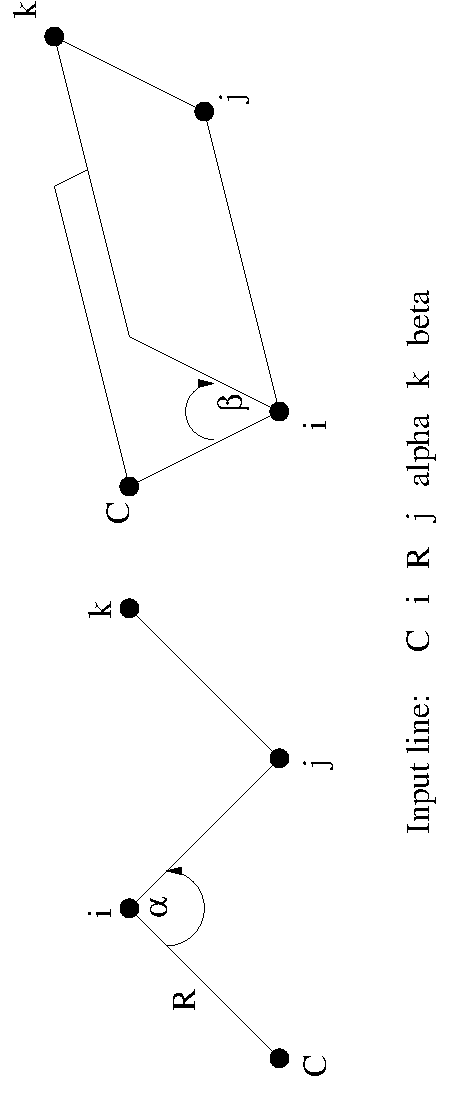
\includegraphics[angle=270,width=6in]{zmat1.eps}
\else
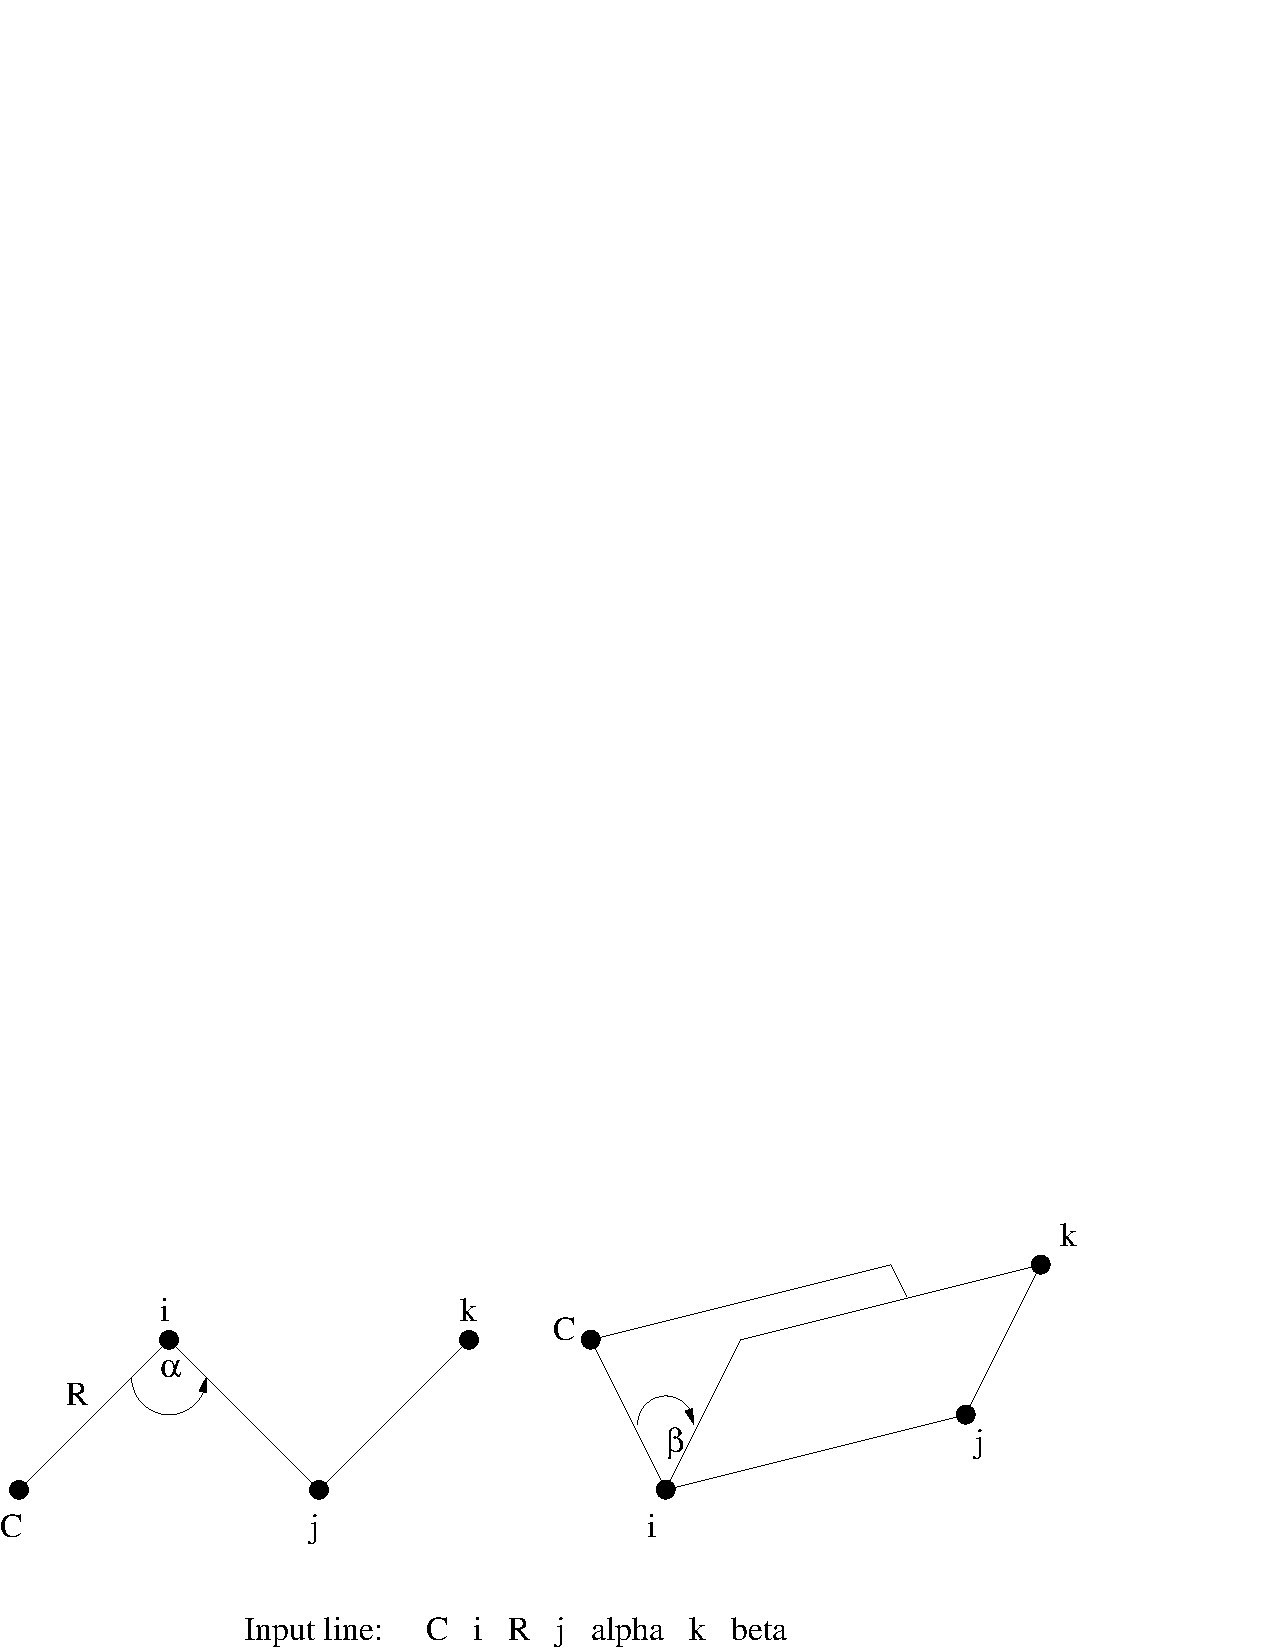
\includegraphics[angle=0,width=6in]{zmat1.pdf}
\fi
\end{latexonly}
\begin{htmlonly}
\psfig{figure=zmat1.eps,angle=270,width=6in}
\end{htmlonly}
\caption{\label{fig:zmat1} Relationships between the centers, bond angle
and dihedral angle in Z-matrix input.}
\end{figure}

\begin{figure}[htbp]
\centering
\begin{latexonly}
\ifx\pdfoutput\undefined
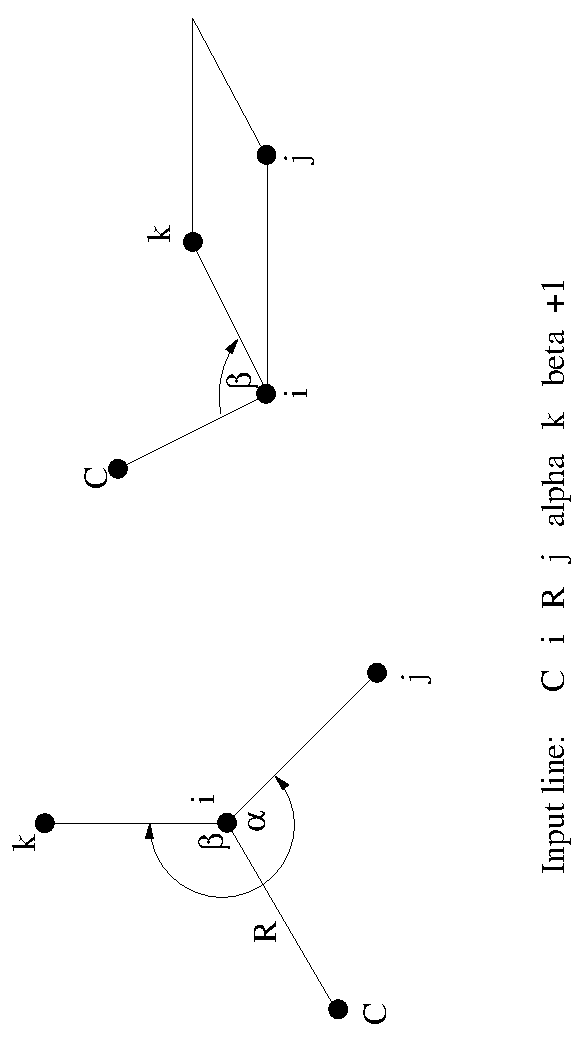
\includegraphics[angle=270,width=6in]{zmat2.eps}
\else
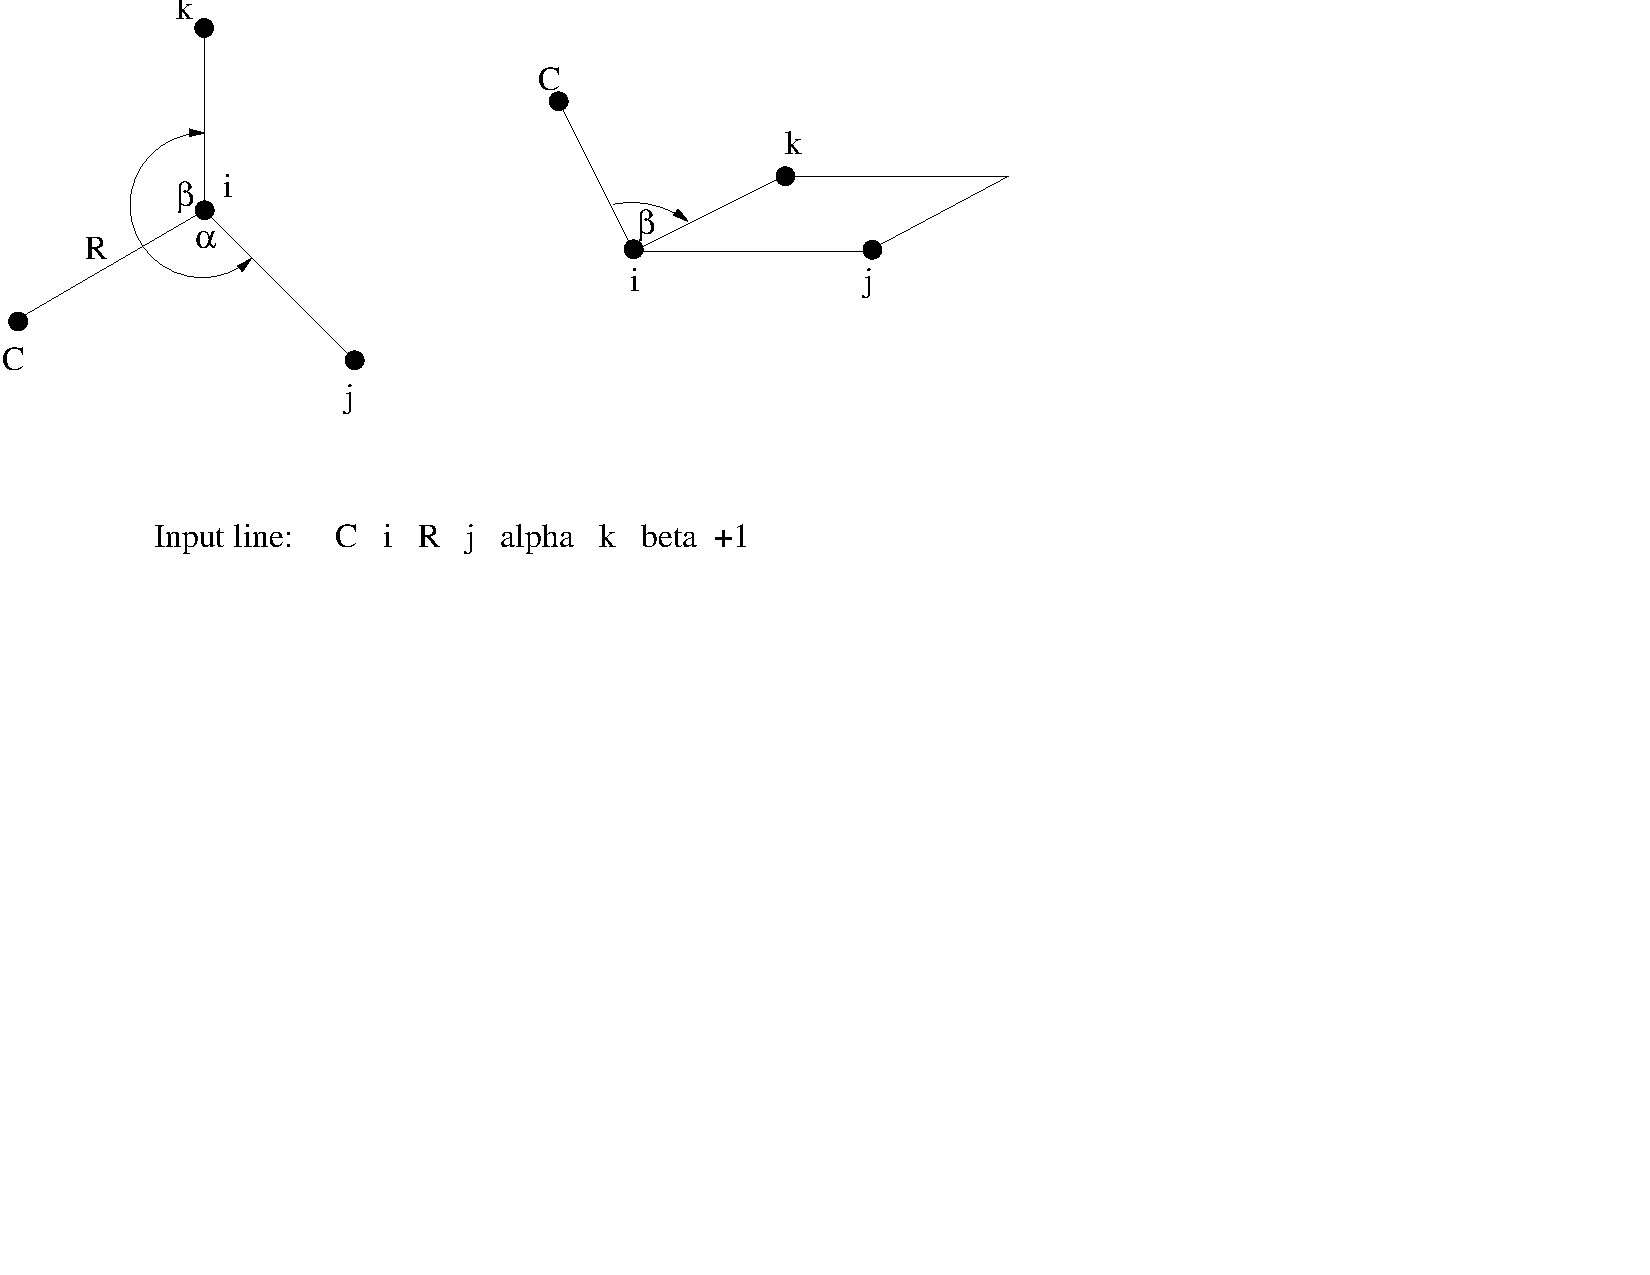
\includegraphics[angle=270,width=6in]{zmat2.pdf}
\fi
\end{latexonly}
\begin{htmlonly}
\psfig{figure=zmat2.eps,angle=270,width=6in}
\end{htmlonly}

\caption{\label{fig:zmat2} Relationships between the centers and two
  bond angles in Z-matrix input with optional parameter specified as $+1$.}
\end{figure}

\begin{figure}[htbp]
\centering
\begin{latexonly}
\ifx\pdfoutput\undefined
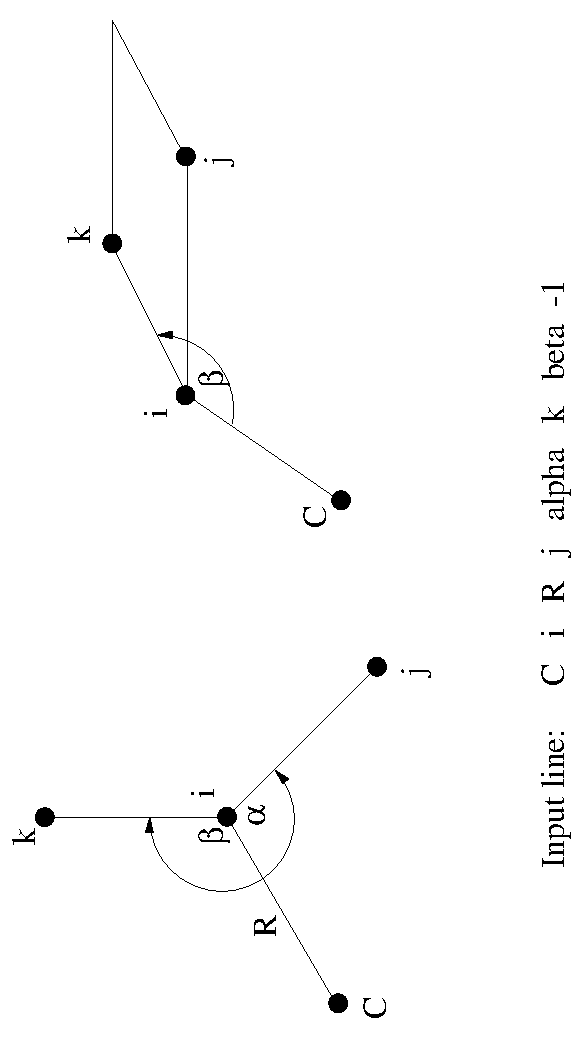
\includegraphics[angle=270,width=6in]{zmat3.eps}
\else
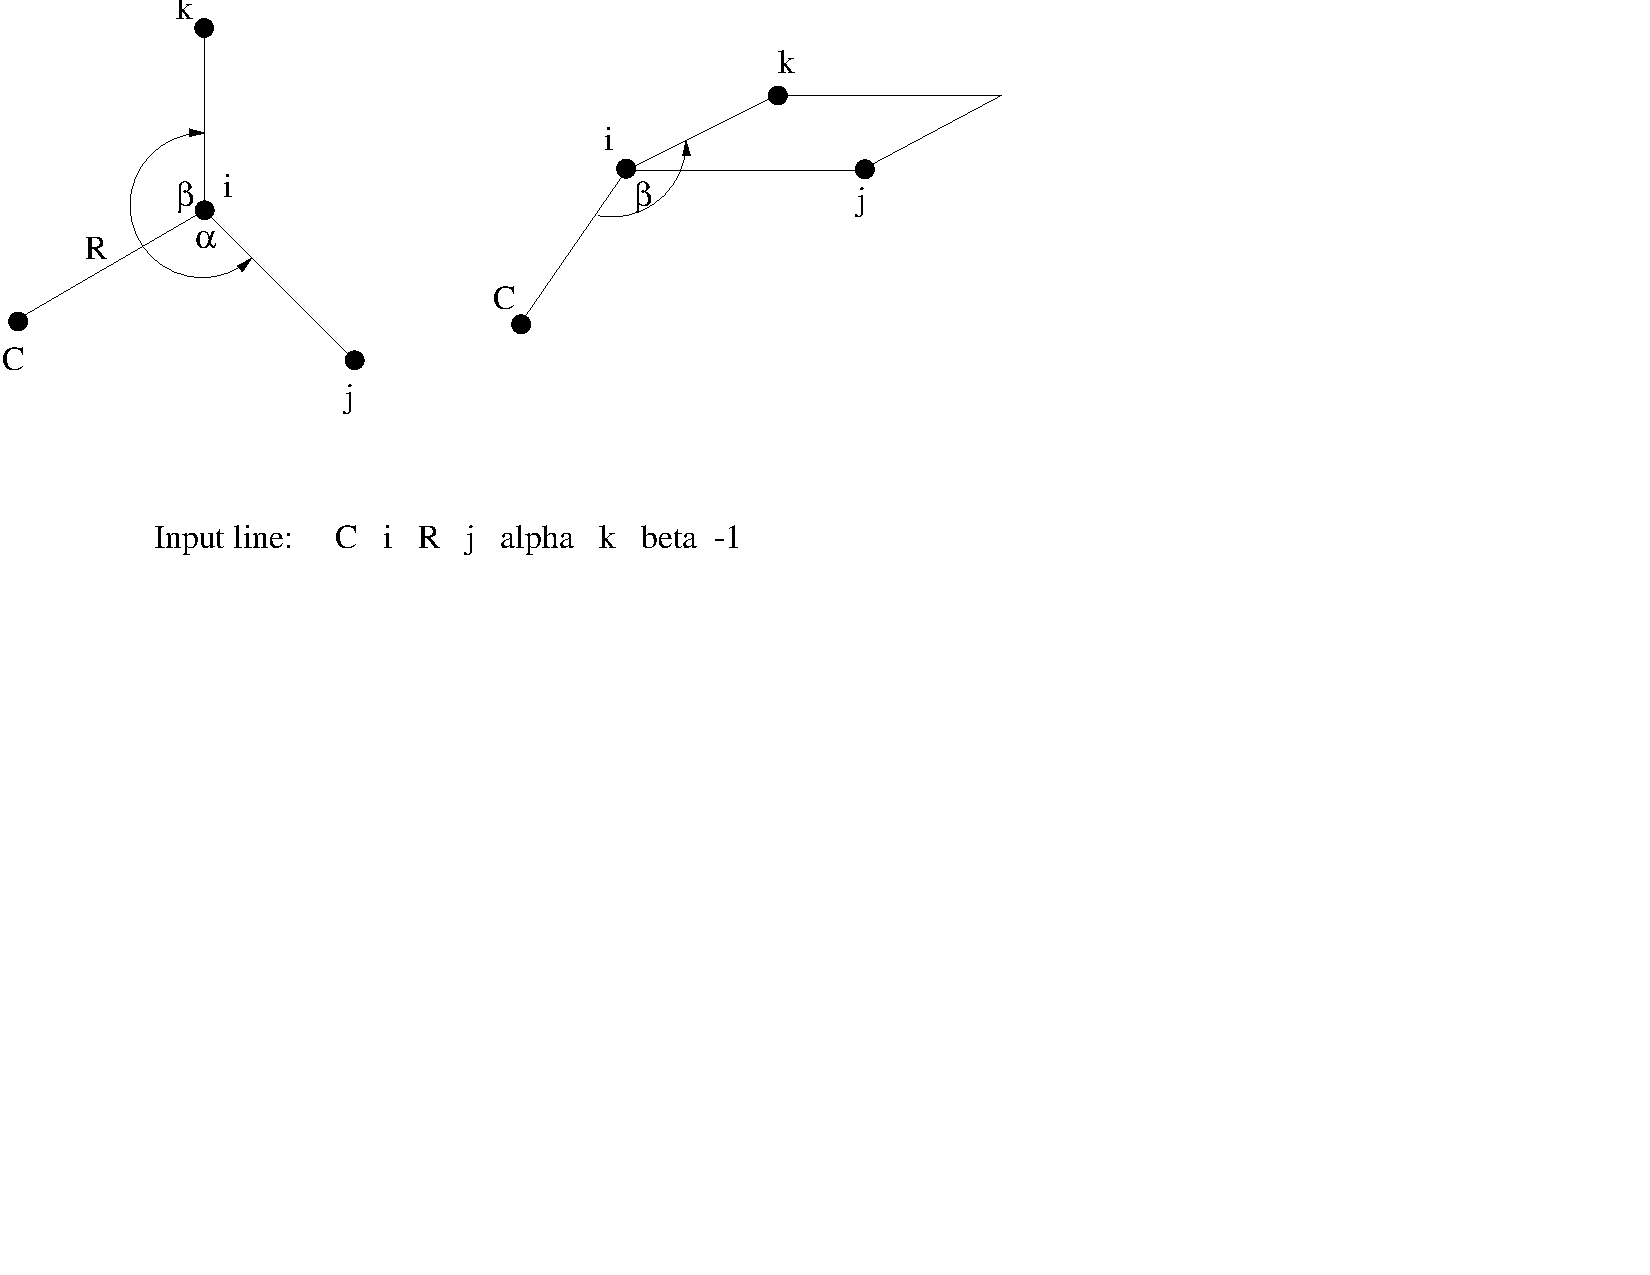
\includegraphics[angle=270,width=6in]{zmat3.pdf}
\fi
\end{latexonly}
\begin{htmlonly}
\psfig{figure=zmat3.eps,angle=270,width=6in}
\end{htmlonly}
\caption{\label{fig:zmat3} Relationships between the centers and two
  bond angles in Z-matrix input with optional parameter specified as $-1$.}
\end{figure}

The Z-matrix input shown above is interpreted as follows:
\begin{enumerate}

   \item \verb+tag1+

   Only  a  tag  is required for the first center.

   \item \verb+tag2 i R+

     The second center requires specification of its tag and the
     bond length ($R_{Ci}$) distance to a previous atom, which is identified by
     \verb+i+.

   \item \verb+tag3 i R j alpha+

     The third center requires specification of its tag, its bond length distance
     ($R_{Ci}$) to one of the two previous centers (identified by the
     value of \verb+i+), and the bond angle $\alpha = \widehat{Cij}$.

   \item \verb+tag i R j alpha k beta [<integer orient default 0>]+

     The fourth, and all subsequent centers, require the tag, a bond
     length ($R_{Ci}$) relative to center \verb+i+, the bond angle with
     centers \verb+i+ and \verb+j+ ($\alpha = \widehat{Cij}$), and {\em either} 
    \begin{enumerate}
    \item the dihedral angle ($\beta$) between the current center and centers
      \verb+i+, \verb+j+, and \verb+k+ (Figure \ref{fig:zmat1}), or
      \item  a second bond angle $\beta = \widehat{Cik}$ and an orientation to 
      the plane containing the other three centers (Figure
      \ref{fig:zmat2} and \ref{fig:zmat3}).
    \end{enumerate}

    By default, $\beta$ is interpreted as a dihedral angle (see Figure
    \ref{fig:zmat1}), but if the optional final parameter (\verb+<orient>+) is
    specified with the value $\pm 1$, then $\beta$ is interpreted as
    the angle $\widehat{Cik}$.  The sign of \verb+<orient>+ specifies the
    direction of the bond angle relative to the plane containing the
    three reference atoms.  If \verb+<orient>+ is $+1$, then the new center
    (\verb+C+) is above the plane (Figure \ref{fig:zmat2}); and if
    \verb+<orient>+ is $-1$, then \verb+C+ is below the plane (Figure
    \ref{fig:zmat3}).
\end{enumerate}

Following the Z-matrix center definitions described above, the user can
 specify initial values for any symbolic variables used to define the
Z-matrix tags.  This is done using the optional  \verb+VARIABLES+ directive,
which has the general form:

%    <string symbol>  <real value> <real value>
\begin{verbatim}
  VARIABLES
    <string symbol>  <real value>
    ...
\end{verbatim}
Each line contains the name of a variable followed by its value.
Optionally, an equals sign (\verb+=+) can be included between the
symbol and its value, for clarity in reading the input file.

%If a second value follows the first value, a second structure gets
%created, built from all the second valued internal coordinates and
%the lone valued internal coordinates for those which are attributed
%only a single vale.  the program will define
%a Linear Synchronous Transit (LST) path between the first structure
%and the second structure ( the initial and final structures respectively).
%A number of structures (11 in total) get created in equal increments
%of the internal coordinates. The set of coordinates get written
%to the file ./xxxx.lst.coord. In an 'LST' task , specified by
%'task <theory> lst', the program calculates the energy of the
%system for all these structures in sequence.

Following the \verb+VARIABLES+ directive, the \verb+CONSTANTS+
directive may be used to define any Z-matrix symbolic variables that remain
unchanged during geometry optimizations. 
To freeze the Cartesian coordinates of an atom, refer
to Section \ref{sec:activeatoms}.  The general form of this directive
is as follows:
\begin{verbatim}
  CONSTANTS
    <string symbol>  <real value>
    ...
\end{verbatim}
Each line contains the name of a variable followed by its value.  As
with the \verb+VARIABLES+ directive, an equals sign (\verb+=+) can be
included between the symbol and its value.

The end of the Z-matrix input using the compound \verb+ZMATRIX+
directive is signaled by a line containing either \verb+END+ or
\verb+ZEND+, following all input for the directive itself and its
associated optional directives.  

A simple example is presented for water.  All Z-matrix parameters are
specified numerically, and symbolic tags are used to specify
connectivity information.  This requires that all tags be unique, and
therefore different tags are used for the two hydrogen atoms, which may 
or may not be identical.  
\begin{verbatim}
  geometry
    zmatrix 
      O
      H1 O 0.95
      H2 O 0.95 H1 108.0
    end
  end
\end{verbatim}

The following example illustrates the Z-matrix input for the molecule
$CH_3CF_3$.  This input uses the numbers of centers to specify
the connectivity information (\verb+i+, \verb+j+, and \verb+k+), and
uses symbolic variables for the Z-matrix parameters {\tt R}, {\tt
  alpha}, and {\tt beta}, which are defined in the inputs for the
\verb+VARIABLES+ and
\verb+CONSTANTS+ directives.

\begin{verbatim}
geometry 
 zmatrix
   C 
   C 1 CC 
   H 1 CH1 2 HCH1 
   H 1 CH2 2 HCH2 3  TOR1 
   H 1 CH3 2 HCH3 3 -TOR2 
   F 2 CF1 1 CCF1 3  TOR3 
   F 2 CF2 1 CCF2 6  FCH1 
   F 2 CF3 1 CCF3 6  -FCH1
   variables
     CC    1.4888 
     CH1   1.0790 
     CH2   1.0789  
     CH3   1.0789  
     CF1   1.3667 
     CF2   1.3669 
     CF3   1.3669
   constants
     HCH1  104.28 
     HCH2  104.74 
     HCH3  104.7 
     CCF1  112.0713 
     CCF2  112.0341 
     CCF3  112.0340 
     TOR1  109.3996 
     TOR2  109.3997 
     TOR3  180.0000 
     FCH1  106.7846 
 end   
end
\end{verbatim}

The input for any centers specified with Cartesian coordinates must
be specified using the format of the \verb+<tag>+ lines described
in Section \ref{sec:cart} above.  However, in
order to correctly specify these Cartesian coordinates 
within the Z-matrix, the user must
understand the orientation of centers specified using
internal coordinates.  These are arranged as follows:
\begin{itemize}
\item The first center is placed at the origin.
\item The second center is placed along the positive z-axis.
\item The third center is placed in the z-x plane.
\end{itemize}

\section{{\tt ZCOORD} --- Forcing internal coordinates}
\label{sec:zcoord}

By default redundant internal coordinates are generated for use in
geometry optimizations.  Connectivity is inferred by comparing
inter-atomic distances with the sum of the van der Waals radii of the
two atoms involved in a possible bond, times a scaling factor. The
scaling factor is an input parameter of \verb+ZCOORD+ which maybe
changed from its default value of 1.3.  Under some circumstances 
(unusual bonding, bond dissociation, \ldots) it will be necessary to
augment the automatically generated list of internal coordinates to
force some specific internal coordinates to be included in among the
internal coordinates.  This is accomplished by including the optional
directive {\tt ZCOORD} within the geometry directive.  The general
form of the \verb+ZCOORD+ directive is as follows:
\begin{verbatim}
  ZCOORD
     CVR_SCALING <real value>
     BOND    <integer i> <integer j> \
             [<real value>] [<string name>] [constant]
     ANGLE   <integer i> <integer j> <integer k> \
             [<real value>] [<string name>] [constant]
     TORSION <integer i> <integer j> <integer k> <integer l> \
             [<real value>] [<string name>] [constant]
  END
\end{verbatim}

The centers \verb+i+, \verb+j+, \verb+k+ and \verb+l+ {\em must} be
specified using the numbers of the centers, as supplied in the input
for the Cartesian coordinates.  The \verb+ZCOORD+ input parameters are
defined as follows:

\begin{itemize}
\item {\tt cvr\_scaling} --- scaling factor applied to van der Waals radii.
\item {\tt bond} --- a bond between the two centers.
\item {\tt angle} --- a bond angle $\widehat{ijk}$.
\item {\tt torsion} --- a torsion (or dihedral) angle.  The
  angle between the planes \verb+i-j-k+ and \verb+j-k-l+.
\end{itemize}   

A value may be specified for a user-defined internal coordinate, in
which case it is forced upon the input Cartesian coordinates while
attempting to make only small changes in the other internal
coordinates.  If no value is provided the value implicit in the input
coordinates is kept.  If the keyword \verb+constant+ is specified, then
that internal variable is not modified during a geometry optimization 
with DRIVER (Section \ref{sec:driver}).  Each internal coordinate may
also be named either for easy identification in the output, or
for the application of constraints (Section \ref{sec:constraints}).

If the keyword \verb+adjust+ is specified on the main \verb+GEOMETRY+
directive, only \verb+ZCOORD+ data may be specified and it can
be used to change the user-defined internal coordinates, including
adding/removing constraints and changing their values.

\section{Applying constraints in geometry optimizations}
\label{sec:activeatoms}
\label{sec:constraints}

Internal coordinates specified as constant in a \verb+ZCOORD+ directive
or in the constants section of a \verb+ZMATRIX+ directive, will be
frozen at their initial values if a geometry optimization is
performed with DRIVER (Section \ref{sec:driver}).

If internal coordinates have the same name (give or take 
an optional sign for torsions) then they are forced to have 
the same value.  This may be used to force bonds or angles to
be equal even if they are not related by symmetry.

When atoms have been specified by their Cartesian coordinates, {\em
and} internal coordinates are not being used, it is possible to freeze
the cartesian position of selected atoms.  This is useful for such
purposes as optimizing a molecule absorbed on the surface of a cluster
with fixed geometry.  Only the gradients associated with the active
atoms are computed.  This can result in a big computational saving,
since gradients associated with frozen atoms are forced to zero (Note,
however, that this destroys the translational and rotational
invariance of the gradient.  This is not yet fully accommodated by the
STEPPER geometry optimization software, and can sometimes result in
slower convergence of the optimization.  The DRIVER optimization
package does not suffer from this problem).

The \verb+SET+ directive (Section \ref{sec:set}) is used to freeze
atoms, by specifying a directive of the form:
\begin{verbatim}
  set geometry:actlist <integer list_of_center_numbers>
\end{verbatim}
This defines only the centers in the list as active.  All other
centers will have zero force assigned to them, and will remain frozen
at their starting coordinates during a geometry optimization.

For example, the following directive specifies that atoms numbered 1,
5, 6, 7, 8, and 15 are active and all other atoms are frozen:
\begin{verbatim}
  set geometry:actlist 1 5:8 15
\end{verbatim}
or equivalently,
\begin{verbatim}
  set geometry:actlist 1 5 6 7 8 15
\end{verbatim}

If this option is not specified by entering a \verb+SET+ directive,
the default behavior in the code is to treat all atoms as active.  To
revert to this default behavior after the option to define frozen
atoms has been invoked, the \verb+UNSET+ directive must be used (since
the database is persistent, see Section \ref{sec:persist}).  The form
of the \verb+UNSET+ directive is as follows:
\begin{verbatim}
  unset geometry:actlist
\end{verbatim}

\section{{\tt SYSTEM} --- Lattice parameters for periodic systems}
\label{sec:latticeparam}

This keyword is needed only for for 1-, 2-, and 3-dimensional
periodic systems.

The {\tt system} keyword can assume the following values

\begin{itemize}
\item {\tt polymer} --- system with 1-d translational symmetry.
\item {\tt surface} --- system with 2-d translational symmetry.
\item {\tt crystal} --- system with 3-d translational symmetry. 
\item {\tt molecule} --- no translational symmetry (this is the default)
\end{itemize}   

When the system possess translational symmetry, {\bf fractional} coordinates
are used in the directions where translational symmetry exists. 
This means that for crystals $x$, $y$ and $z$ are fractional, for
surfaces $x$ and $y$  are fractional, whereas for polymers only $z$ is
fractional.
For example, in the following H$_2$O layer input (a 2-d  periodic
system), $x$ and $y$ coordinates are fractional, whereas $z$
is expressed in \AA .
\begin{verbatim}
geometry units angstrom
  O     0.353553    0.353553         2.100000000
  H     0.263094    0.353553         2.663590000
  H     0.444007    0.353553         2.663590000
\end{verbatim}

Since no space group symmetry is available yet other than $P1$, input
of cell parameters is relative to the primitive cell. For example,
this is the input  required for the cubic face-centered type structure
of bulk MgO.

\begin{verbatim}

  system crystal
   lat_a 2.97692 lat_b 2.97692 lat_c 2.97692 
   alpha 60.00 beta 60.00 gamma 60.00
  end
\end{verbatim}





%%% Local Variables: 
%%% mode: latex
%%% TeX-master: "user"
%%% End: 


\chapter{Basis sets}
%
% $Id$
%
\label{sec:basis} 

NWChem currently supports basis sets consisting of generally
contracted\footnote{Generally contracted meaning that the same
  primitive, Gaussian functions are contracted into multiple
  contracted functions using different contraction coefficients.
  Reuse of the radial functions increases the efficiency of integral
  generation.} Cartesian Gaussian functions up to a maximum angular
 momentum of six ($h$ functions), and also $sp$ (or L)
functions\footnote{An $sp$ shell is two-component general contraction.
  However, the first component specifies an $s$ shell and the second a
  $p$ shell.  Again, reuse of the radial functions increases the efficiency
  of integral generation.} .  The {\tt BASIS} directive is used to
define these, and also to specify use of an effective core potential
(ECP) that is associated with a basis set; see Section \ref{sec:ecp}.

The basis functions to be used for a given calculation can be drawn
from a standard set in the EMSL basis set library that is included in
the release of NWChem  (See Appendix \ref{sec:knownbasis} for a list
of the standard basis sets currently supplied with the release of the
code).  Alternatively, the user can specify particular functions
explicitly in the input, to define a particular basis set.

The general form of the \verb+BASIS+ directive is as follows:

\begin{verbatim}
  BASIS [<string name default "ao basis">] \
        [(spherical || cartesian) default cartesian] \
        [(segment || nosegment) default segment] \
        [(print || noprint) default print]
        [rel]

     <string tag> library [<string tag_in_lib>] \
                  <string standard_set> [file <filename>] \
                  [except <string tag list>] [rel]

        ...

     <string tag> <string shell_type> [rel]
        <real exponent> <real list_of_coefficients>
        ...
     
  END
\end{verbatim}    

Examining the keywords on the first line of the \verb+BASIS+ directive:


\begin{itemize}
\item {\tt name}

  By default, the basis set is stored in the database with the name
  \verb+"ao basis"+.  Another name may be specified in the \verb+BASIS+
  directive, thus, multiple basis sets may be stored simultaneously in the
  database.  Also, the DFT (Section \ref{sec:dft}) 
  and RI-MP2 (Section \ref{sec:rimp2}) modules and the
  Dyall-modified-Dirac relativistic method (Section \ref{sec:dyall-mod-dir})
  require multiple basis sets with specific names.

The user can associate the \verb+"ao basis"+ with another named basis
using the \verb+SET+ directive (see Section \ref{sec:set}).  

\item {{\tt SPHERICAL} or {\tt CARTESIAN}}

The keywords \verb+spherical+ and \verb+cartesian+ offer the option of
using either spherical-harmonic (5 d, 7 f, 9 g, \ldots) or Cartesian
(6 d, 10 f, 15 g, \ldots) angular functions.  The default is
Cartesian.  

Note that the correlation-consistent basis sets were designed using
spherical harmonics and to use these, the \verb+spherical+ keyword
should be present in the \verb+BASIS+ directive.  The use of spherical
functions also helps eliminate problems with linear dependence.


\item {{\tt SEGMENT} or {\tt NOSEGMENT}}

By default, NWChem forces all basis sets to be segmented, 
even if they are input with general contractions or $L$ or sp
shells. This is because the current derivative integral program cannot
handle general contractions.  If a calculation is  
computing energies only, a 
performance gain can result from exploiting generally contracted basis
sets, in which case {\tt NOSEGMENT} should be specified.

\item {{\tt PRINT} or {\tt NOPRINT}}

The default is for the input module to print all basis sets encountered.
Specifying the keyword \verb+noprint+ allows the user to suppress this output.

\item {{\tt REL}}

This keyword marks the entire basis as a relativistic basis for the purposes
of the Dyall-modified-Dirac relativistic integral code. The marking of the
basis set is necessary for the code to make the proper association between
the relativistic shells in the ao basis and the shells in the large and/or
small component basis. This is only necessary for basis sets which are to be
used as the ao basis. The user is referred to Section \ref{sec:dyall-mod-dir}  
for more details.

\end{itemize}

Basis sets are associated with centers by using the tag of a center in
a geometry that has either been input by the user (Section
\ref{sec:geom}) or is available elsewhere.  Each atom or center with
the same \verb+tag+ will have the same basis set.  All atoms must have
basis functions assigned to them --- only dummy centers (X or Bq) may have no
basis functions.  To facilitate the specification of the geometry and
the basis set for any chemical system, the matching process of a basis
set tag to a geometry tag first looks for an exact match.  If no match
is found, NWChem will attempt to match, ignoring case, the name or
symbol of the element.  E.g., all hydrogen atoms in a system could be
labeled ``H1'', ``H2'', \ldots, in the geometry but only
one basis set specification for ``H'' or ``hydrogen'' is necessary.
If desired, a special basis may be added to one or more centers (e.g.,
``H1'') by providing a basis for that tag.
If the matching mechanism fails then NWChem stops with an appropriate
error message.

A special set of tags, ``*'' and tags ending with a ``*'' (E.g. ``H*'')
can be used in combination with the keyword \verb+library+ (see section
below). These tags facilitate the definition of a certain type of basis 
set of all atoms, or a group of atoms, in a geometry using only a single 
%<<<<<<< basis.tex
or very few basis set entries. The ``*'' tag will not place basis sets 
on dummy atoms, Bq* can be used for that if necessary.
%=======
%or very few basis set entries. The ``*'' tag will not place basis sets 
%on dummy atoms, Bq* can be used for that if necessary. 
%>>>>>>> 1.25

Examined next is how to reference standard basis sets in the basis set
library, and finally, how to define a basis set using exponents and
coefficients.

\section{Basis set library}

The keyword \verb+library+ associated with each specific \verb+tag+
entry specifies that the calculation will use the standard basis set
in NWChem for that center.  The variable \verb+<standard_set>+ is the
name that identifies the functions in the library.  The names of
standard basis sets are not case sensitive.  See Appendix
\ref{sec:knownbasis} for a complete list of the basis sets in the
NWChem library and their specifications.  

The general form of the input line requesting basis sets from the NWChem
basis set library is:
\begin{verbatim}
     <string tag> library [<string tag_in_lib>] \
                  <string standard set> [file < filename> \
                  [except <string tag list>] [rel]
        ...
\end{verbatim}

For example, the NWChem basis set library contains the Dunning cc-pvdz
basis set.  These may be used as follows
\begin{verbatim}
  basis
    oxygen library cc-pvdz
    hydrogen library cc-pvdz
  end
\end{verbatim}

A default path of the NWChem basis set libraries is provided on installation 
of the code, but a different path can be defined by specifying the keyword 
\verb+file+, and one can explicitly name the file to be accessed
for the basis functions. For example,
\begin{verbatim}
  basis
    o  library 3-21g file /usr/d3g681/nwchem/library
    si library 6-31g file /usr/d3g681/nwchem/libraries/
  end
\end{verbatim}
This directive tells the code to use the basis set \verb+3-21g+ in
the file {\tt /usr/\-d3g681/\-nwchem/\-library} for atom \verb+o+ and
to use the basis set \verb+6-31g+ in the directory 
{\tt /usr/\-d3g681/\-nwchem/\-libraries/} for atom \verb+si+, rather 
than look for them in the default libraries. When a directory is defined 
the code will search for the basis set in a file with the name {\tt 6-31g}.

The ``*'' tag can be used to efficiently define basis set input directives 
for large numbers of atoms. An example is:
\begin{verbatim}
  basis
    *  library 3-21g
  end
\end{verbatim}
This directive tells the code to assign the basis sets \verb+3-21g+ to
all the atom tags defined in the geometry. If one wants to place a
different basis set on one of the atoms defined in the geometry, the 
following directive can be used:
\begin{verbatim}
  basis
    *  library 3-21g except H
  end
\end{verbatim}
This directive tells the code to assign the basis sets \verb+3-21g+ to
all the atoms in the geometry, except the hydrogen atoms. Remember that 
the user will have to explicitly define the hydrogen basis set in this
directive! One may also define tags that end with a ``*'': 
\begin{verbatim}
  basis
    oxy*  library 3-21g 
  end
\end{verbatim}
This directive tells the code to assign the basis sets \verb+3-21g+ to 
all atom tags in the geometry that start with ``oxy''.

If standard basis sets are to be placed upon a dummy center, the
variable \verb+<tag_in_lib>+ must also be entered on this line, to
identify the correct atom type to use from the basis function library
(see the ghost atom example in Section \ref{sec:set} and below).  For
example: To specify the cc-pvdz basis for a calculation on the water
monomer in the dimer basis, where the dummy oxygen and dummy hydrogen
centers have been identified as \verb+bqo+ and \verb+bqh+
respectively, the \verb+BASIS+ directive is as follows:

\begin{verbatim}
  basis
    o   library cc-pvdz
    h   library cc-pvdz
    bqo library o cc-pvdz
    bqh library h cc-pvdz
  end
\end{verbatim}
A special dummy center tag is \verb+bq*+, which will assign the same basis 
set to all bq centers in the geometry. Just as with the ``*'' tag, the 
\verb+except+ list can be used to assign basis sets to unique dummy centers.

The library basis sets can also be marked as relativistic by adding the
\verb+rel+ keyword to the tag line. See Section \ref{sec:dyall-mod-dir} for
more details. The correlation consistent basis sets have been contracted for
relativistic effects and are included in the standard library.

There are also contractions in the standard library for both a point nucleus
and a finite nucleus of Gaussian shape. These are usually distinguished by
the suffixex {\tt \_pt} and {\tt \_fi}. It is the user's responsibility to
ensure that the contraction matches the nuclear type specified in the
geometry object. The specification of a finite nucleus basis set does NOT
automatically set the nuclear type for that atom to be finite.  See 
Section \ref{sec:geom} for information.

\section{Explicit basis set definition}

If the basis sets in the library or available in other external files
are not suitable for a given calculation, 
the basis set may be explicitly defined.
A generally contracted Gaussian basis function is associated with a
center using an input line of the following form:
\begin{verbatim}
     <string tag> <string shell_type> [rel]
        <real exponent> <real list_of_coefficients>
        ...
\end{verbatim}

The variable \verb+<shell_type>+ identifies the angular momentum of the
shell, $s$, $p$, $d$, \ldots.  NWChem is configured to handle up to $h$
shells.  The keyword \verb+rel+ marks the shell as relativistic --- see
Section \ref{sec:dyall-mod-dir} for more details.  Subsequent lines define
the primitive function exponents and contraction coefficients.  General
contractions are specified by including multiple columns of coefficients.

The following example defines basis sets for the water molecule:
\begin{verbatim}
  basis spherical nosegment
    oxygen s
      11720.0000    0.000710  -0.000160
       1759.0000    0.005470  -0.001263
        400.8000    0.027837  -0.006267
        113.7000    0.104800  -0.025716
         37.0300    0.283062  -0.070924
         13.2700    0.448719  -0.165411
          5.0250    0.270952  -0.116955
          1.0130    0.015458   0.557368
          0.3023   -0.002585   0.572759
    oxygen s                
          0.3023    1.000000
    oxygen p                
         17.7000    0.043018
          3.8540    0.228913
          1.0460    0.508728
          0.2753    0.460531
    oxygen p                
          0.2753    1.000000
    oxygen d
          1.1850    1.000000
    hydrogen s
         13.0100    0.019685
          1.9620    0.137977
          0.4446    0.478148
          0.1220    0.501240
    hydrogen s  
          0.1220    1.000000
    hydrogen p  
          0.7270    1.000000
    oxygen s
          0.01      1.0
    hydrogen s
          0.02974   1.0
    hydrogen p
          0.141      1.0
  end
\end{verbatim}


\section{Combinations of library and explicit basis set input}
The user can use a mixture of library basis and explicit basis set
input to define the basis sets used on the various atoms.

For example, the following \verb+BASIS+ directive augments the Dunning
cc-pvdz basis set for the water molecule with a diffuse s-shell on
oxygen and adds the aug-cc-pVDZ diffuse functions onto the hydrogen.
\begin{verbatim}
  basis spherical nosegment
    oxygen library cc-pvdz
    hydrogen library cc-pvdz
    oxygen s
      0.01 1.0
    hydrogen library "aug-cc-pVDZ Diffuse"
  end
\end{verbatim}

The resulting basis set defined is identical to the one defined above 
in the explicit basis set input.



\chapter{Effective Core Potentials}
%
% $Id$
%
\label{sec:ecp}
\def\ell{l}
Effective core potentials (ECPs) are a useful means of replacing the core
electrons in a calculation with an effective potential, thereby eliminating
the need for the core basis functions, which usually require a large set of
Gaussians to describe them. In addition to replacing the core, they may be
used to represent relativistic effects, which are largely confined to the
core. In this context, both the scalar (spin-free) relativistic effects and
spin-orbit (spin-dependent) relativistic effects may be included in
effective potentials. NWChem has the facility to use both, and these are
described in the next two sections.

A brief recapitulation of the development of RECPs is given here, following
Pacios and Christiansen\footnote{l.~F.~Pacios and P.~A.~Christiansen,
J.~Chem.~Phys.~{\bf 82}, 2664 (1985)}. The process can be viewed as starting
from an atomic Dirac-Hartree-Fock calculation, done in {\it jj} coupling,
and producing relativistic effective potentials (REPs) for each $\ell$ and
$j$ value, $U^{\rm REP}_{\ell j}$.  From these, a local potential is
extracted, which for example contains the Coulomb potential of the core
electrons balanced by the part of the nuclear attraction which cancels the
core electron charge. The residue is expressed in a semi-local form,
\begin{equation}
U^{\rm REP} = U^{\rm REP}_{LJ}(r) + \sum_{\ell=0}^{L-1}
\sum_{j=|\ell-1/2}^{\ell+1/2} \left[ U^{\rm REP}_{\ell j}(r) -  
U^{\rm REP}_{LJ}(r) \right] \sum_m | \ell j m \rangle \langle \ell j m |
\end{equation}
where $L$ is one larger than the maximum angular momentum in the atom.
The scalar potential is obtained by averaging the REPs for each $j$ for a
given $\ell$ to give an averaged relativistic effective potential, or AREP,
\begin{equation}
U^{\rm AREP}_\ell(r) = \frac{1}{2\ell+1} \left[ \ell U^{\rm REP}_{\ell-1/2}(r)
+ (\ell+1) U^{\rm REP}_{\ell+1/2}(r) \right].
\end{equation}
These are summed into the full potential.
%\begin{equation}
%U^{\rm AREP} = U^{\rm AREP}_{L}(r) + \sum_{\ell=0}^{L-1}
%\left[ U^{\rm AREP}_{\ell}(r) -  U^{\rm AREP}_{L}(r)
%\sum_m | \ell m \rangle \langle \ell m |.
%\end{equation}

The spin-orbit potential is obtained from the difference between the REPs
for the two $j$ values for a given \ell, and may be 
represented in terms of an effective spin-orbit operator,
\begin{equation}
H^{\rm SO} = {\bf s} \cdot \sum_{\ell=1}^{L-1} \frac{2}{2\ell+1} 
\Delta U^{\rm REP}_{\ell} \sum_{mm'} 
| \ell m \rangle \langle \ell m | \hat\ell | \ell m' \rangle \langle \ell m' |.
\end{equation}
where
\begin{equation}
\Delta U^{\rm REP}_{\ell} = U^{\rm REP}_{\ell+1/2}(r)
 - U^{\rm REP}_{\ell-1/2}(r).
\end{equation}
The spin-orbit integrals generated by NWChem are the integrals over the sum,
including the factor of $2/(2\ell+1)$, so that they may be treated as an
effective spin-orbit operator without further factors introduced.

The effective potentials, both scalar and spin-orbit, are fitted to
Gaussians with the form
\[
 r^2U_l(r) = \sum_{k} A_{lk} r^{n_{lk}} e^{-B_{lk}r^{2}}
\]
where $A_{lk}$ is the contraction coefficient, $n_{lk}$ is the
exponent of the ``r'' term (r-exponent), and $B_{lk}$ is the Gaussian
exponent.  The $n_{lk}$ is shifted by 2, in accordance with most of the ECP
literature and implementations, i.e., an $n_{lk} = 0$ implies
$r^{-2}$.  The current implementation allows $n_{lk}$ values
of only 0, 1, or 2. 

\section{Scalar ECPs}
\label{sec:scalar_ecp}

The optional directive \verb+ECP+ allows the user to describe an effective core
potential (ECP) in terms of contracted Gaussian functions as given above.
Potentials using these functions must be specified explicitly by user input
in the \verb+ECP+ directive.  This directive has essentially the same form
and properties as the standard \verb+BASIS+ directive, except for essential
differences required for ECPs.  Because of this, the ECP is treated
internally as a basis set. The form of the input for the
\verb+ECP+ directive is as follows:

%        [spherical || cartesian default cartesian]
%        [segment || nosegment default segment] 

\begin{verbatim}
  ECP [<string name default "ecp basis">] \
        [print || noprint default print]

     <string tag> library [<string tag_in_lib>] \
                  <string standard_set> [file <filename>] \
                  [except <string tag list>]

     <string tag> [nelec] <integer number_of_electrons_replaced>
 
        ...

     <string tag> <string shell_type>
     <real r-exponent> <real Gaussian-exponent> <real list_of_coefficients>
        ...
     
  END
\end{verbatim}    

ECPs are automatically segmented, even if general contractions are input.
The projection operators defined in an ECP are spherical by default, so
there is no need to include the \verb+CARTESIAN+ or \verb+SPHERICAL+ keyword
as there is for a standard basis set.  ECPs are associated with centers in
geometries through tags or names of centers.  These tags must match in the
same manner as for basis sets the tags in a \verb+GEOMETRY+ and
\verb+ECP+ directives, and are limited to sixteen (16) characters.
Each center with the same tag will have the same ECP.  By default, the
input module prints each ECP that it encounters.  The \verb+NOPRINT+
option can be used to disable printing.  There can be only one active
ECP, even though several may exist in the input deck.  The ECP modules
load ``ecp basis'' inputs along with any ``ao basis'' inputs present.
ECPs may be used in both energy and gradient calculations.

ECPs are named in the same fashion as geometries or regular basis
sets, with the default name being \verb+"ecp basis"+.  It should be
clear from the above discussion on geometries and database entries how
indirection is supported.  All directives that are in common with the
standard Gaussian basis set input have the same function and syntax.

As for regular basis sets, ECPs may be obtained from the standard library.
The names of the sets of ECPs available in the standard
library (their coverage is described in Appendix \ref{sec:knownbasis}) are
\begin{itemize}
\item \verb,"Hay-Wadt MB (n+1) ECP",
\item \verb,"Hay-Wadt VDZ (n+1) ECP",
\item \verb+"LANL2DZ ECP"+
\item \verb+"SBKJC VDZ ECP"+
\item \verb+"Stuttgart RLC ECP"+
\item \verb+"Stuttgart RSC ECP"+
\item \verb+"CRENBL ECP"+
\item \verb+"CRENBS ECP"+
\end{itemize}

The keyword \verb+nelec+ allows the user to specify the number of core
electrons replaced by the ECP.  Additional input lines define the
specific coefficients and exponents.  The variable \verb+<shell_type>+
is used to specify the components of the ECP.  The keyword \verb+ul+
entered for \verb+<shell_type>+ denotes the local part of the ECP.
This is equivalent to the highest angular momentum functions specified
in the literature for most ECPs.  The standard entries (\verb+s, p, d+,
etc.) for \verb+shell_type+ specify the angular momentum projector
onto the local function.  The shell type label of \verb+s+ indicates
the \verb+ul-s+ projector input, \verb+p+ indicates the \verb+ul-p+,
etc.

For example, the Christiansen, Ross and Ermler ARECPs are available in
the standard basis set libary named \verb+{crenbl_ecp}+.  To perform a
calculation on uranyl (UO$_2^{2+}$) with all-electron oxygen
(aug-cc-pvdz basis), and uranium with an ARECP and using the
corresponding basis the following input can be used
\begin{verbatim}
  geometry
    U 0 0  0
    O 0 0  1.65
    O 0 0 -1.65
  end
  basis 
    U library crenbl_ecp
    O library aug-cc-pvdz
  end
  ecp
    U library crenbl_ecp
  end
\end{verbatim}

The following is an example of explicit input of an ECP for H$_2$CO.
It defines an ECP for the carbon and oxygen atoms in the molecule.

% \centerline{{\bf H$_2$CO }}

\begin{verbatim}
  ecp
    C nelec 2 # ecp replaces 2 electrons on C
    C ul      # d
            1       80.0000000       -1.60000000
            1       30.0000000       -0.40000000
            2        0.5498205       -0.03990210
   C s        # s - d 
            0        0.7374760        0.63810832
            0      135.2354832       11.00916230
            2        8.5605569       20.13797020
    C p       # p - d
            2       10.6863587       -3.24684280
            2       23.4979897        0.78505765
    O nelec 2 # ecp replaces 2 electrons on O
    O ul      # d 
            1       80.0000000       -1.60000000
            1       30.0000000       -0.40000000
            2        1.0953760       -0.06623814
    O s       # s - d
            0        0.9212952        0.39552179
            0       28.6481971        2.51654843
            2        9.3033500       17.04478500
    O p       # p - s 
            2       52.3427019       27.97790770
            2       30.7220233      -16.49630500
  end
\end{verbatim}

Various ECPs without a local function are available, including those of 
the Stuttgart group. For those, no "ul" part needs to be defined. To 
define the absence of the local potential, simply specify one contraction
with a zero coefficient:

\begin{verbatim}
     <string tag> ul
     2     1.00000     0.00000
\end{verbatim}

\section{Spin-orbit ECPs}
\label{sec:spinorb_ecp}

The Spin-orbit ECPs can be used with the Density Functional Approach, but 
one has to run the calculations without symmetry. Note: when a Hartree-Fock
method is specified the spin-orbit input will be ignored.

Spin-orbit ECPs are fitted in precisely the same functional form as the
scalar RECPs and have the same properties, with the exception that there is
no local potential ul, no $s$ potential and no effective charge has to be
defined. Spin-orbit potentials are
specified in the same way as ECPs except that the directive \verb+SO+ is
used instead of \verb+ECP+. Note that there currently are no spin-orbit
ECPs defined in the standard NWChem library.  The \verb+SO+ 
directive is as follows:

\begin{verbatim}
  SO [<string name default "so basis">] \
        [print || noprint default print]

     <string tag> library [<string tag_in_lib>] \
                  <string standard_set> [file <filename>]
                  [except <string tag list>]
        ...

     <string tag> <string shell_type>
     <real r-exponent> <real Gaussian-exponent> <real list_of_coefficients>
        ...
     
  END
\end{verbatim}    

Note: in the literature the coefficients of the spin-orbit potentials are NOT 
always defined in the same manner. The NWChem code assumes that the spin-orbit
potential defined in the input is of the form:
\begin{equation}
\Delta U^{\rm NWChem}_{\ell} = \frac{2}{2\ell+1} \Delta U_{\ell} 
\end{equation}
For example, in the literature the Stuttgart potentials are defined as 
$\Delta U_{\ell}$ and, hence, have to be multiplied by $2/(2{\ell}+1)$. On the 
other hand, the CRENBL potentials in the published papers are defined as 
$\frac{\ell}{2\ell+1} \Delta U_{\ell}$ and, hence, have to be multiplied by 
$2/{\ell}$ (Warning: on the CRENBL website the spin-orbit potentials already
have been corrected with the $2/{\ell}$ factor).

%RJH: Align six comment symbols (#) with the other two.--fmr.
%Generally contracted ECP basis sets are not in wide use, but the
%functionality has been included in NWChem for applications where they
%might be useful. 



\chapter{Relativistic All-electron Approximations}
%
% $Id$
%
\label{sec:rel}
All methods which include treatment of relativistic effects are ultimately
based on the Dirac equation, which has a four component wave function. The
solutions to the Dirac equation describe both positrons (the ``negative
energy'' states) and electrons (the ``positive energy'' states), as well as
both spin orientations, hence the four components. The wave function may be
broken down into two-component functions traditionally known as the large
and small components; these may further be broken down into the spin
components. 

The implementation of approximate all-electron relativistic methods in
quantum chemical codes requires the removal of the negative energy states
and the factoring out of the spin-free terms. Both of these may be achieved
using a transformation of the Dirac Hamiltonian known in general as a
Foldy-Wouthuysen transformation. Unfortunately this transformation cannot be
represented in closed form for a general potential, and must be
approximated.  One popular approach is that originally formulated by Douglas
and Kroll\footnote{M.~Douglas and N.~M.~Kroll, Ann. Phys. (N.Y.)  {\bf 82},
89 (1974)} and developed by Hess\footnote{B.A.~Hess, Phys.~Rev.~A~{\bf 32},
756 (1985); {\bf 33}, 3742 (1986)}. This approach decouples the positive and
negative energy parts to second order in the external potential (and also
fourth order in the fine structure constant, $\alpha$). Other approaches include 
the Zeroth Order Regular Approximation (ZORA)\footnote{C.~Chang, M.~Pelissier, 
M.~Durand, Physica Scripta ~{\bf 34}, 294 (1986); E.~van Lenthe, ~{\it The ZORA Equation}, 
doctoral thesis, Vrije Universiteit, Amsterdam (1996); S.~Faas, J.G.~Snijders, 
J.H.~van Lenthe, E.~van Lenthe, and E.J.~Baerends, Chem.~Phys.~ Lett.~{\bf 246}, 632 (1995).}
and modification of the Dirac equation by Dyall\footnote{K.~G.~Dyall,
J.~Chem.~Phys.~{\bf 100}, 2118 (1994)}, and involves an exact FW
transformation on the atomic basis set level\footnote{K.~G.~Dyall,
J.~Chem.~Phys.~{\bf 106}, 9618 (1997); K.~G.~Dyall and T.~Enevoldsen,
J.~Chem.~Phys.~{\bf 111}, 10000 (1999).}.

Since these approximations only modify the integrals, they can in principle
be used at all levels of theory. At present the Douglas-Kroll and ZORA 
implementations can be used at all levels of theory whereas 
Dyall's approach is currently available at the Hartree-Fock level. 
The derivatives have been implemented, allowing both methods to be used in 
geometry optimizations and frequency calculations.

The \verb+RELATIVISTIC+ directive provides input for the implemented relativistic 
approximations and is a compound directive that encloses additional directives 
specific to the approximations:
\begin{verbatim}
  RELATIVISTIC
   [DOUGLAS-KROLL [<string (ON||OFF) default ON> \
                 <string (FPP||DKH||DKFULL||DK3||DK3FULL) default DKH>]  ||
    ZORA [ (ON || OFF) default ON ] || 
    DYALL-MOD-DIRAC [ (ON || OFF) default ON ] 
                  [ (NESC1E || NESC2E) default NESC1E ] ]
   [CLIGHT <real clight default 137.0359895>]
  END
\end{verbatim}

Only one of the methods may be chosen at a time.  If both methods are found
to be on in the input block, NWChem will stop and print an error message.
There is one general option for both methods, the definition of the speed 
of light in atomic units:

\begin{verbatim}
  CLIGHT <real clight default 137.0359895>
\end{verbatim}

The following sections describe the optional sub-directives that
can be specified within the \verb+RELATIVISTIC+ block.

\section{Douglas-Kroll approximation}
\label{sec:douglas-kroll}

The spin-free and spin-orbit one-electron Douglas-Kroll 
approximation have been implemented. The use of relativistic effects 
from this Douglas-Kroll approximation can be invoked by specifying:

\begin{verbatim}
  DOUGLAS-KROLL [<string (ON||OFF) default ON> \
                 <string (FPP||DKH||DKFULL|DK3|DK3FULL) default DKH>]
\end{verbatim}

The \verb+ON|OFF+ string is used to turn on or off the
Douglas-Kroll approximation.  By default, if the \verb+DOUGLAS-KROLL+
keyword is found, the approximation will be used in the calculation.
If the user wishes to calculate a non-relativistic quantity after turning
on Douglas-Kroll, the user will need to define a new \verb+RELATIVISTIC+
block and turn the approximation \verb+OFF+.  The user could also simply
put a blank \verb+RELATIVISTIC+ block in the input file and all options 
will be turned off.

The \verb+FPP+ is the approximation based on free-particle projection 
operators\footnote{B.A.~Hess, Phys.~Rev.~A~{\bf 32}, 756 (1985)} whereas the 
\verb+DKH+ and \verb+DKFULL+ approximations are based on external-field 
projection operators\footnote{B.A.~Hess, Phys.~Rev.~A~{\bf 33}, 3742 (1986)}.
The latter two are considerably better approximations than the former. \verb+DKH+ 
is the Douglas-Kroll-Hess approach and is the approach that is generally 
implemented in quantum chemistry codes. \verb+DKFULL+ includes certain 
cross-product integral terms ignored in the \verb+DKH+ approach (see for example 
H\"{a}berlen and R\"{o}sch\footnote{O.D.~H\"{a}berlen, N.~R\"{o}sch, 
Chem.~Phys.~Lett.~{\bf 199}, 491 (1992)}). The third-order Douglas-Kroll 
approximation has been implemented by T. Nakajima and K. Hirao\footnote{T. Nakajima 
and K. Hirao, Chem.~Phys.~Lett.~{\bf 329}, 5111 (2000); T. Nakajima and K. Hirao, 
J.~Chem.~Phys.~{\bf 113}, 7786 (2000)}. This approximation can be called using
\verb+DK3+ (DK3 without cross-product integral terms) or \verb+DK3FULL+ (DK3 with
cross-product integral terms).

The contracted basis sets used in the calculations should reflect the relativistic
effects, i.e. one should use contracted basis sets which were generated using the 
Douglas-Kroll Hamiltonian. Basis sets that were contracted using the 
non-relativistic (Sch\"{o}dinger) Hamiltonian WILL PRODUCE ERRONEOUS RESULTS for
elements beyond the first row. See appendix \ref{sec:knownbasis} for available
basis sets and their naming convention.

NOTE: we suggest that spherical basis sets are used in the calculation. The use of 
high quality cartesian basis sets can lead to numerical inaccuracies.

In order to compute the integrals needed for the Douglas-Kroll approximation
the implementation makes use of a fitting basis set (see literature given
above for details). The current code will create this fitting basis set
based on the given {\tt "ao basis"} by simply uncontracting that basis. This
again is what is commonly implemented in quantum chemistry codes that
include the Douglas-Kroll method.  Additional flexibility is available to
the user by explicitly specifying a Douglas-Kroll fitting basis
set. This basis set must be named {\tt "D-K basis"} (see Chapter
\ref{sec:basis}).

\section{Zeroth Order regular approximation (ZORA)}
\label{sec:zora}

The spin-free and spin-orbit one-electron zeroth-order regular approximation (ZORA) 
have been implemented. The use of relativistic effects with ZORA 
can be invoked by specifying:

\begin{verbatim}
  ZORA [<string (ON||OFF) default ON>
\end{verbatim}

The \verb+ON|OFF+ string is used to turn on or off ZORA.  
By default, if the \verb+ZORA+ keyword is found, the approximation 
will be used in the calculation. If the user wishes to calculate 
a non-relativistic quantity after turning on ZORA, the user 
will need to define a new \verb+RELATIVISTIC+ block and turn 
the approximation \verb+OFF+.  The user can also simply put 
a blank \verb+RELATIVISTIC+ block in the input file and all options 
will be turned off.

\section{Dyall's Modified Dirac Hamitonian approximation}
\label{sec:dyall-mod-dir}

The approximate methods described in this section are all based on Dyall's
modified Dirac Hamiltonian. This Hamiltonian is entirely equivalent to the
original Dirac Hamiltonian, and its solutions have the same properties.
The modification is achieved by a transformation on the small component,
extracting out \hbox{$\sigma\cdot{\bf p}/2mc$}. This gives the modified small
component the same symmetry as the large component, and in fact it differs
from the large component only at order $\alpha^2$.  The advantage of the
modification is that the operators now resemble the operators of the
Breit-Pauli Hamiltonian, and can be classified in a similar fashion into
spin-free, spin-orbit and spin-spin terms. It is the spin-free terms which
have been implemented in NWChem, with a number of further approximations.

The first is that the negative energy states are removed by a normalized
elimination of the small component (NESC), which is equivalent to an exact
Foldy-Wouthuysen (EFW) transformation. The number of components in the wave
function is thereby effectively reduced from 4 to 2. NESC on its own does
not provide any advantages, and in fact complicates things because the
transformation is energy-dependent. The second approximation therefore
performs the elimination on an atom-by-atom basis, which is equivalent to
neglecting blocks which couple different atoms in the EFW transformation.
The advantage of this approximation is that all the energy dependence can be
included in the contraction coefficients of the basis set.  The tests which
have been done show that this approximation gives results well within
chemical accuracy. The third approximation neglects the commutator of the
EFW transformation with the two-electron Coulomb interaction, so that the
only corrections that need to be made are in the one-electron integrals.
This is the equivalent of the Douglas-Kroll(-Hess) approximation as it is
usually applied.

The use of these approximations can be invoked with the use of the
\verb+DYALL-MOD-DIRAC+ directive in the \verb+RELATIVISTIC+ directive block.
The syntax is as follows.

\begin{verbatim}
  DYALL-MOD-DIRAC [ (ON || OFF) default ON ] 
                  [ (NESC1E || NESC2E) default NESC1E ]
\end{verbatim}

The \verb+ON|OFF+ string is used to turn on or off the
Dyall's modified Dirac approximation. By default, if the \verb+DYALL-MOD-DIRAC+
keyword is found, the approximation will be used in the calculation.
If the user wishes to calculate a non-relativistic quantity after turning
on Dyall's modified Dirac, the user will need to define a new 
\verb+RELATIVISTIC+
block and turn the approximation \verb+OFF+.  The user could also simply
put a blank \verb+RELATIVISTIC+ block in the input file and all options 
will be turned off.

Both one- and two-electron approximations are available
\verb+NESC1E || NESC2E+, and both have
analytic gradients. The one-electron approximation is the default.
The two-electron approximation specified by \verb+NESC2E+ has some sub
options which are placed on the same logical line as the
\verb+DYALL-MOD-DIRAC+ directive, with the following syntax:

\begin{verbatim}
  NESC2E [ (SS1CENT [ (ON || OFF) default ON ] || SSALL) default SSALL ]
         [ (SSSS [ (ON || OFF) default ON ] || NOSSSS) default SSSS ]
\end{verbatim}

The first sub-option gives the capability to limit the two-electron
corrections to those in which the small components in any density must be on
the same center.  This reduces the $(LL|SS)$ contributions to at most
three-center integrals and the $(SS|SS)$ contributions to two centers. For a
case with only one relativistic atom this option is redundant. The second
controls the inclusion of the $(SS|SS)$ integrals which are of order
$\alpha^4$. For light atoms they may safely be neglected, but for heavy
atoms they should be included. 

In addition to the selection of this keyword in the \verb+RELATIVISTIC+
directive block, it is necessary to supply basis sets in addition to the
\verb+ao basis+. For the one-electron approximation, three basis sets are
needed: the atomic FW basis set, the large component basis set and the small
component basis set. The atomic FW basis set should be included in the
\verb+ao basis+.
The large and small components should similarly be incorporated
in basis sets named \verb+large component+ and \verb+small component+,
respectively. For the two-electron approximation, only two basis sets are
needed. These are the large component and the small component. The large component
should be included in the \verb+ao basis+ and the small component
is specified separately as \verb+small component+, as for the one-electron
approximation. This means that the two approximations can {\it not} be run
correctly without changing the \verb+ao basis+, and it is up to the user to
ensure that the basis sets are correctly specified.

There is one further requirement in the specification of the basis sets. In
the \verb+ao basis+, it is necessary to add the \verb+rel+ keyword either to the
\verb+basis+ directive or the library tag line (See below for examples). 
The former marks the basis
functions specified by the tag as relativistic, the latter marks the whole
basis as relativistic. The marking is actually done at the unique shell
level, so that it is possible not only to have relativistic and
nonrelativistic atoms, it is also possible to have relativistic and
nonrelativistic shells on a given atom. This would be useful, for example,
for diffuse functions or for high angular momentum correlating functions,
where the influence of relativity was small. The marking of shells as
relativistic is necessary to set up a mapping between the ao basis and the
large and/or small component basis sets. For the one-electron approximation
the large and small component basis sets MUST be of the same size and
construction, i.e. differing only in the contraction coefficients.

It should also be noted that the relativistic code will NOT work with basis
sets that contain sp shells, nor will it work with ECPs. Both of these are
tested and flagged as an error.

Some examples follow. The first example sets up the data for relativistic
calculations on water with the one-electron approximation and the
two-electron approximation, using the library basis sets.

\begin{verbatim}
  start h2o-dmd

  geometry units bohr
  symmetry c2v
    O       0.000000000    0.000000000   -0.009000000
    H       1.515260000    0.000000000   -1.058900000
    H      -1.515260000    0.000000000   -1.058900000
  end

  basis "fw" rel
    oxygen library cc-pvdz_pt_sf_fw
    hydrogen library cc-pvdz_pt_sf_fw
  end

  basis "large"
    oxygen library cc-pvdz_pt_sf_lc
    hydrogen library cc-pvdz_pt_sf_lc
  end

  basis "large2" rel
    oxygen library cc-pvdz_pt_sf_lc
    hydrogen library cc-pvdz_pt_sf_lc
  end

  basis "small"
    oxygen library cc-pvdz_pt_sf_sc
    hydrogen library cc-pvdz_pt_sf_sc
  end

  set "ao basis" fw
  set "large component" large
  set "small component" small

  relativistic
    dyall-mod-dirac
  end

  task scf

  set "ao basis" large2
  unset "large component"
  set "small component" small

  relativistic
    dyall-mod-dirac nesc2e
  end

  task scf
\end{verbatim}

The second example has oxygen as a relativistic atom and hydrogen nonrelativistic.

\begin{verbatim}
  start h2o-dmd2

  geometry units bohr
  symmetry c2v
    O       0.000000000    0.000000000   -0.009000000
    H       1.515260000    0.000000000   -1.058900000
    H      -1.515260000    0.000000000   -1.058900000
  end

  basis "ao basis"
    oxygen library cc-pvdz_pt_sf_fw rel
    hydrogen library cc-pvdz
  end

  basis "large component"
    oxygen library cc-pvdz_pt_sf_lc
  end

  basis "small component"
    oxygen library cc-pvdz_pt_sf_sc
  end

  relativistic
    dyall-mod-dirac
  end

  task scf
\end{verbatim}


\chapter{Hartree-Fock or Self-consistent Field} 
%
% $Id$
%
\label{sec:scf}

The NWChem self-consistent field (SCF) module computes closed-shell
restricted Hartree-Fock (RHF) wavefunctions, restricted high-spin
open-shell Hartree-Fock (ROHF) wavefunctions, and spin-unrestricted
Hartree-Fock (UHF) wavefunctions.

The \verb+SCF+ directive provides input to the SCF module and is a
compound directive that encloses additional directives specific to the
SCF module:
\begin{verbatim}
  SCF
    ...
  END
\end{verbatim}

\section{Wavefunction type}

A spin-restricted, closed shell RHF calculation is performed by
default.  An error results if the number of electrons is inconsistent
with this assumption.  The number of electrons is inferred from the
total charge on the system and the sum of the effective nuclear
charges of all centers (atoms and dummy atoms, Section
\ref{sec:geom}).  The total charge on the system is zero by default,
unless specified at some value by input on the \verb+CHARGE+ directive
(Section \ref{sec:toplevel}).

The options available to define the SCF wavefunction and multiplicity
are as follows:

\begin{verbatim}
  SINGLET 
  DOUBLET 
  TRIPLET 
  QUARTET 
  QUINTET 
  SEXTET
  SEPTET
  OCTET
  NOPEN <integer nopen default 0>
  RHF
  ROHF
  UHF
\end{verbatim}

The optional keywords \verb+SINGLET+, \verb+DOUBLET+, \ldots,
\verb+OCTET+ and \verb+NOPEN+ allow the user to specify the number of
singly occupied orbitals for a particular calculation.  \verb+SINGLET+
is the default, and specifies a closed shell; \verb+DOUBLET+ specifies
one singly occupied orbital; \verb+TRIPLET+ specifies two singly
occupied orbitals; and so forth.  If there are more than seven singly
occupied orbitals, the keyword \verb+NOPEN+ must be used, with the
integer \verb+nopen+ defining the number of singly occupied
orbitals (sometimes referred to as open shells).

If the multiplicity is any value other than \verb+SINGLET+, the
default calculation will be a spin-restricted, high-spin, open-shell
SCF calculation (keyword ROHF).  The open-shell orbitals must be the
highest occupied orbitals.  If necessary, any starting vectors may be
rearranged through the use of the \verb+SWAP+ keyword on the
\verb+VECTORS+ directive (see Section \ref{sec:vectors}) to accomplish
this.

A spin-unrestricted solution can also be performed by specifying the
keyword \verb+UHF+.  In UHF calculations, it is assumed that the
number of singly occupied orbitals corresponds to the difference
between the number of alpha-spin and beta-spin orbitals.  For example,
a UHF calculation with 2 more alpha-spin orbitals than beta-spin
orbitals can be obtained by specifying

\begin{verbatim}
  scf
     triplet ; uhf    # (Note: two logical lines of input)
     ...
  end
\end{verbatim}

The user should be aware that, by default, molecular orbitals are
symmetry adapted in NWChem.  This may not be desirable for fully
unrestricted wavefunctions.  In such cases, the user has the option of
defeating the defaults by specifying the keywords \verb+ADAPT OFF+
(see Section \ref{sec:adapt}) and \verb+SYM OFF+ (see Section
\ref{sec:sym}).

The keywords \verb+RHF+ and \verb+ROHF+ are provided in the code for
completeness. It may be necessary to specify these in order to modify
the behavior of a previous calculation (see Section \ref{sec:persist}
for restart behavior).

\section{{\tt SYM} --- use of symmetry}
\label{sec:sym}

 \begin{verbatim}
   SYM <string (ON||OFF) default ON>
 \end{verbatim}

This directive enables/disables the use of symmetry to speed up Fock matrix
construction (via the petite-list or skeleton algorithm) in the SCF, if
symmetry was used in the specification of the geometry.  Symmetry
adaptation of the molecular orbitals is not affected by this option.
The default is to use symmetry if it is specified in the geometry
directive (Section \ref{sec:geom}). 

For example, to disable use of symmetry in Fock matrix construction:
\begin{verbatim}
  sym off
\end{verbatim}

\section{{\tt ADAPT} -- symmetry adaptation of MOs}
\label{sec:adapt}

\begin{verbatim}
  ADAPT <string (ON||OFF) default ON>
\end{verbatim}

The default in the SCF module calculation is to force symmetry
adaption of the molecular orbitals. This does not affect the speed of
the calculation, but without explicit adaption the resulting orbitals
may be symmetry contaminated for some problems.  This is especially
likely if the calculation is started using orbitals from a distorted
geometry.

The underlying assumption in the use of symmetry in Fock matrix
construction is that the density is totally symmetric.  If the orbitals
are symmetry contaminated, this assumption may not be valid --- which
could result in incorrect energies and poor convergence of the
calculation.  It is thus advisable when specifying \verb+ADAPT OFF+ to
also specify \verb+SYM OFF+ (Section \ref{sec:sym}).

\section{{\tt TOL2E} --- integral screening threshold}
\label{sec:tol2e}

\begin{verbatim}
  TOL2E <real tol2e default min(10e-7 , 0.01*$thresh$)>
\end{verbatim}

The variable \verb+tol2e+ is used in determining the integral
screening threshold for the evaluation of the energy and related
Fock-like matrices.  The Schwarz inequality is used to screen the
product of integrals and density matrices in a manner that results in
an accuracy in the energy and Fock matrices that approximates the
value specified for \verb+tol2e+. 

It is generally not necessary to set this parameter directly.  Specify
instead the required precision in the wavefunction, using the
\verb+THRESH+ directive (Section \ref{sec:thresh}). The default
threshold is the minimum of $10^{-7}$ and 0.01 times the requested
convergence threshold for the SCF calculation (Section
\ref{sec:thresh}).  

The input to specify the threshold explicitly within the \verb+SCF+
directive is, for example:

\begin{verbatim}
  tol2e 1e-9
\end{verbatim}

For very diffuse basis sets, or for high-accuracy calculations it
might be necessary to set this parameter.  A value of $10^{-12}$ is
sufficient for nearly all such purposes.

\section{{\tt VECTORS} --- input/output of MO vectors}
\label{sec:vectors}


\begin{verbatim}
  VECTORS [[input] (<string input_movecs default atomic>) || \
                   (project <string basisname> <string filename>) || \
                   (fragment <string file1> [<string file2> ...])] \
          [swap [alpha||beta] <integer vec1 vec2> ...] \
          [reorder <integer atom1 atom2> ...] \
          [output <string output_filename default input_movecs>] \
          [lock]
          [rotate  <string input_geometry> <string input_movecs>] 
\end{verbatim}

The \verb+VECTORS+ directive allows the user to specify the source and
destination of the molecular orbital vectors.  In a startup
calculation (see Section \ref{sec:start}), the default source for
guess vectors is a diagonalized Fock matrix constructed from a
superposition of the atomic density matrices for the particular
problem.  This is usually a very good guess.  For a restarted 
calculation, the default is to use the previous MO vectors.

The optional keyword \verb+INPUT+ allows the user to specify the
source of the input molecular orbital vectors as any of the following:
\begin{itemize}
\item \verb+ATOMIC+ --- eigenvectors of a Fock-like matrix formed from
  a superposition of the atomic densities (the default guess).  See
  Sections \ref{sec:atomscf} and \ref{sec:tolguess}.  
\item \verb+HCORE+ --- eigenvectors of the bare-nucleus Hamiltonian or
  the one-electron Hamiltonian.
\item \verb+filename+ --- the name of a file containing the MO vectors
  from a previous calculation.  Note that unless the path is fully
  qualified, or begins with a dot (``.''), then it is assumed to
  reside in the directory for permanent files (see Section
  \ref{sec:dirs}).
\item \verb+PROJECT basisname filename+ --- projects the existing MO
  vectors in the file \verb+filename+ from the smaller basis with name
  \verb+basisname+ into the current basis.  The definition of the
  basis \verb+basisname+ must be available in the current database,
  and the basis must be smaller than the current basis.  In addition,
  the geometry used for the previous calculations must have the atoms
  in the same order and in the same orientation as the current
  geometry.
\item \verb+FRAGMENT file1 ...+ --- assembles starting MO vectors from
  previously performed calculations on fragments of the system and is
  described in more detail in Section \ref{sec:fragguess}.  Even
  though there are some significant restrictions in the use of the
  initial implementation of this method (see Section
  \ref{sec:fragguess}), this is the most powerful initial guess option
  within the code.  It is particularly indispensable for open shell
  metallic systems.
\item \verb+ROTATE input_geometry input_movecs+ --- rotates 
   MO vectors generated at a previous geometry 
   to the current active geometry.
\end{itemize}
 
The molecular orbitals are saved every iteration if more than 600
seconds have elapsed, and also at the end of the calculation.  At
completion (converged or not), the SCF module always canonically
transforms the molecular orbitals by {\em separately} diagonalizing
the closed--closed, open--open, and virtual--virtual blocks of the
Fock matrix.

The name of the file used to store the MO vectors is determined as
follows:
\begin{itemize}
\item if the \verb+OUTPUT+ keyword was specified on the \verb+VECTORS+
  directive, then the filename that follows this keyword is used, or
\item if the input vectors were read from a file, this file is reused
  for the output vectors (overwriting the input vectors); else,
\item a default file name is generated in the directory for permanent
  files (Section \ref{sec:dirs}) by prepending \verb+".movecs"+ with
  the file prefix, i.e., \verb+"<file_prefix>.movecs"+.
\end{itemize}
The name of this file is stored in the database so that a subsequent
SCF calculation will automatically restart from these MO vectors.

Applications of this directive are illustrated in the following
examples.

Example 1:
\begin{verbatim}
  vectors output h2o.movecs
\end{verbatim}
Assuming a start-up calculation, this directive will result in use of
the default atomic density guess, and will output the vectors to the
file \verb+h2o.movecs+.

Example 2:
\begin{verbatim}
  vectors input initial.movecs output final.movecs
\end{verbatim}
This directive will result in the initial vectors being read from the
file \verb+"initial.movecs"+.  The results will be written to the file
\verb+final.movecs+.  The contents of \verb+"initial.movecs"+ will not
be changed.

Example 3:
\begin{verbatim}
  vectors input project "small basis" small.movecs
\end{verbatim}
This directive will cause the calculation to start from vectors in the
file \verb+"small.movecs"+ which are in a basis named \verb+"small basis"+.
The output vectors will be written to the default file
\verb+"<file_prefix.movecs>"+.
 
Once starting vectors have been obtained using any of the possible
options, they may be reordered through use of the \verb+SWAP+ keyword.
This optional keyword requires a list of orbital pairs that will be
swapped.  For UHF calculations, separate \verb+SWAP+ keywords may be
provided for the alpha and beta orbitals, as necessary.

An example of use of the \verb+SWAP+ directive:
\begin{verbatim}
  vectors input try1.movecs swap 173 175 174 176 output try2.movecs
\end{verbatim}
This directive will cause the initial orbitals to be read from the
file \verb+"try1.movecs"+.  The vectors for the orbitals within the
pairs 173--175 will be swapped with those within 174--176, so the
resulting order is 175, 176, 173, 174.  The final orbitals obtained in
the calculation will be written to the file \verb+"try2.movecs"+.

The swapping of orbitals occurs as a sequential process in the order
(left to right) input by the user.  Thus, regarding each pair as an
elementary transposition it is possible to construct arbitrary
permutations of the orbitals.  For instance, to apply the permutation
$(6 7 8 9)$\footnote{The cyclic permutation $(6 7 8 9)$ maps the
  ordered list {\tt 6 7 8 9} into {\tt 9 6 7 8}.} we note that this
permutation is equal to $(6 7)(7 8)(8 9)$, and thus may be specified
as
\begin{verbatim}
  vectors swap 8 9  7 8  6 7
\end{verbatim}

Another example, now illustrating this feature for a UHF calculation,
is the directive
\begin{verbatim}
  vectors swap beta 4 5 swap alpha 5 6
\end{verbatim}
This input will result in the swapping of the 5--6 alpha orbital pair
and the 4--5 beta orbital pair.  (All other items in the input use the
default values.)

The \verb+LOCK+ keyword allows the user to specify that the ordering
of orbitals will be locked to that of the initial vectors, insofar as
possible. The default is to order by ascending orbital energies within
each orbital space. One application where locking might be desirable
is a calculation where it is necessary to preserve the ordering of a
previous geometry, despite flipping of the orbital energies.  For such
a case, the \verb+LOCK+ directive can be used to prevent the SCF
calculation from changing the ordering, even if the orbital energies
change.

The mapping of the MO's to the nuclei can be changed using the \verb+REORDER+ keyword.
Once starting vectors have been obtained using any of the possible
options, the \verb+REORDER+ keyword moves the MO coefficients between atoms
listed in the integer list.  This keyword is particularly useful for calculating localized
electron and hole states.

This optional keyword requires a list containing the new atom ordering.
It is not necessary to provide separate lists for alpha and 
beta orbitals. 

An example of use of the \verb+REORDER+ keyword:
\begin{verbatim}
  vectors input try1.movecs reorder 2 1 output try2.movecs
\end{verbatim}
This directive will cause the initial orbitals to be read from the
file \verb+"try1.movecs"+.  The MO coefficients for the basis functions
on atom 2 
will be swapped with those on atom 1.
The final orbitals obtained in
the calculation will be written to the file \verb+"try2.movecs"+.

The following example shows how the \verb+ROTATE+ keyword can be used to rotate
MO vectors calculated at geometry \verb+geom1+ to geometry \verb+geom2+, which has a 
different rotational orientation:

\begin{verbatim}
set geometry geom1
dft
 vectors input atomic output geom1.mo
end
task dft

set geometry geom2
dft
 vectors input rotate geom1 geom1.mo output geom2.mo
end
task dft

\end{verbatim}
\subsection{Superposition of fragment molecular orbitals}
\label{sec:fragguess}

The fragment initial guess is particularly useful in the following
instances:
\begin{itemize}
\item The system naturally decomposes into molecules that can be
  treated individually, e.g., a cluster.
\item One or more fragments are particularly hard to converge and
  therefore much time can be saved by converging them independently.
\item A fragment (e.g., a metal atom) must be prepared with a specific
  occupation.  This can often be readily accomplished with a
  calculation on the fragment using dummy charges to model a ligand
  field.
\item The molecular occupation predicted by the atomic initial guess
  is often wrong for systems with heavy metals which may have
  partially occupied orbitals with lower energy than some doubly
  occupied orbitals.  The fragment initial guess avoids this problem.
\end{itemize}

\begin{verbatim}
  VECTORS [input] fragment <string file1> [<string file2> ...]
\end{verbatim}
The molecular orbitals are formed by superimposing the previously
generated orbitals of fragments of the molecule being studied.  These
fragment molecular orbitals must be in the same basis as the current
calculation.  The input specifies the files containing the fragment
molecular orbitals.  For instance, in a calculation on the water
dimer, one might specify
\begin{verbatim}
  vectors fragment h2o1.movecs h2o2.movecs
\end{verbatim}
where \verb+h2o1.movecs+ contains the orbitals for the first fragment, and
\verb+h2o2.movecs+ contains the orbitals for the second fragment.

A complete example of the input for a calculation on the water
dimer using the fragment guess is as follows:
\begin{verbatim}
   start dimer

   title "Water dimer SCF using fragment initial guess"

   geometry dimer
     O   -0.595   1.165  -0.048
     H    0.110   1.812  -0.170
     H   -1.452   1.598  -0.154
     O    0.724  -1.284   0.034
     H    0.175  -2.013   0.348
     H    0.177  -0.480   0.010
   end

   geometry h2o1
     O   -0.595   1.165  -0.048
     H    0.110   1.812  -0.170
     H   -1.452   1.598  -0.154
   end

   geometry h2o2
     O    0.724  -1.284   0.034
     H    0.175  -2.013   0.348
     H    0.177  -0.480   0.010
   end

   basis
     o library 3-21g
     h library 3-21g
   end

   set geometry h2o1
   scf; vectors input atomic output h2o1.movecs; end
   task scf

   set geometry h2o2
   scf; vectors input atomic output h2o2.movecs; end
   task scf

   set geometry dimer
   scf
   vectors input fragment h2o1.movecs h2o2.movecs \
           output dimer.movecs
   end
   task scf
\end{verbatim}
First, the geometry of the dimer and the two monomers are specified
and given names.  Then, after the basis specification, calculations
are performed on the fragments by setting the geometry to the
appropriate fragment (Section \ref{sec:set}) and redirecting the
output molecular orbitals to an appropriately named file.  Note also
that use of the atomic initial guess is forced, since the default
initial guess is to use any existing MOs which would not be
appropriate for the second fragment calculation.  Finally, the dimer
calculation is performed by specifying the dimer geometry, indicating
use of the fragment guess, and redirecting the output MOs.

The following points are important in using the fragment initial guess:
\begin{enumerate}
\item The fragment calculations must be in the same basis set as the
  full calculation.
\item The order of atoms in the fragments and the order in which the
  fragment files are specified must be such that when the fragment
  basis sets are concatenated all the basis functions are in the same
  order as in the full system.  This is readily accomplished by first
  generating the full geometry with atoms for each fragment
  contiguous, splitting this into numbered fragments and specifying
  the fragment MO files in the correct order on the \verb+VECTORS+
  directive.
\item The occupation of orbitals is preserved when they are merged
  from the fragments to the full molecule and the resulting occupation
  must match the requested occupation for the full molecule.  E.g., a
  triplet ROHF calculation must be comprised of fragments that have
  a total of exactly two open-shell orbitals. 
\item Because of these restrictions, it is not possible to introduce
  additional atoms (or basis functions) into fragments for the purpose
  of cleanly breaking real bonds.  However, it is possible, and highly
  recommended, to introduce additional point charges to simulate the
  presence of other fragments.
\item MO vectors of partially occupied or strongly polarized systems
  are very sensitive to orientation.  While it is possible to specify
  the same fragment MO vector file multiple times in the
  \verb+VECTORS+ directive, it is usually much better to do a separate
  calculation for each fragment.
\item Linear dependencies which were present in a fragment calculation
  may be magnified in the full calculation.  When this occurs, 
  some of the fragment's highest virtual orbitals will not be copied to the
  full system, and a warning will be printed.
  
\end{enumerate}

A more involved example is now presented.  We wish to model the sextet
state of Fe(III) complexed with water, imidazole and a heme with a net
unit positive charge.  The default atomic guess does not give the
correct $d^5$ occupation for the metal and also gives an incorrect
state for the double anion of the heme.  The following performs
calculations on all of the fragments.  Things to note are:
\begin{enumerate}
\item The use
of a dummy $+2$ charge in the initial guess on the heme which in part
simulates the presence of the metal ion, and also automatically forces
an additional two electrons to be added to the system (the default net
charge being zero).
\item The iron fragment calculation (charge +3, $d^5$, sextet) will
  yield the correct open-shell occupation for the full system.  If,
  instead, the {\it d}-orbitals were partially occupied (e.g., the doublet
  state) it would be useful to introduce dummy charges around the iron
  to model the ligand field and thereby lift the degeneracy to obtain
  the correct occupation.
\item $C_s$ symmetry is used for all of the calculations.  It is not
  necessary that the same symmetry be used in  all of the
  calculations, provided that the order and orientation of the atoms 
  is preserved.
\item The \verb+unset scf:*+ directive is used immediately before
  the calculation on the full system so that the default name for the
  output MO vector file can be used, rather than having to specify it
  explicitly.
\end{enumerate}
\begin{verbatim}
start heme6a1
title  "heme-H2O (6A1) from M.Dupuis"

############################################################
# Define the geometry of the full system and the fragments #
############################################################

geometry full-system
   symmetry cs

   H     0.438   -0.002    4.549
   C     0.443   -0.001    3.457
   C     0.451   -1.251    2.828
   C     0.452    1.250    2.828
   H     0.455    2.652    4.586
   H     0.461   -2.649    4.586
   N1    0.455   -1.461    1.441
   N1    0.458    1.458    1.443
   C     0.460    2.530    3.505
   C     0.462   -2.530    3.506
   C     0.478    2.844    1.249
   C     0.478    3.510    2.534
   C     0.478   -2.848    1.248
   C     0.480   -3.513    2.536
   C     0.484    3.480    0.000
   C     0.485   -3.484    0.000
   H     0.489    4.590    2.664
   H     0.496   -4.592    2.669

   H     0.498    4.573    0.000
   H     0.503   -4.577    0.000
   H    -4.925    1.235    0.000
   H    -4.729   -1.338    0.000
   C    -3.987    0.685    0.000
   N    -3.930   -0.703    0.000
   C    -2.678    1.111    0.000
   C    -2.622   -1.076    0.000
   H    -2.284    2.126    0.000
   H    -2.277   -2.108    0.000
   N    -1.838    0.007    0.000

   Fe    0.307    0.000    0.000

   O     2.673   -0.009    0.000
   H     3.238   -0.804    0.000
   H     3.254    0.777    0.000
end

geometry ring-only
   symmetry cs
   H     0.438   -0.002    4.549
   C     0.443   -0.001    3.457
   C     0.451   -1.251    2.828
   C     0.452    1.250    2.828
   H     0.455    2.652    4.586
   H     0.461   -2.649    4.586
   N1    0.455   -1.461    1.441
   N1    0.458    1.458    1.443
   C     0.460    2.530    3.505
   C     0.462   -2.530    3.506
   C     0.478    2.844    1.249
   C     0.478    3.510    2.534
   C     0.478   -2.848    1.248
   C     0.480   -3.513    2.536
   C     0.484    3.480    0.000
   C     0.485   -3.484    0.000
   H     0.489    4.590    2.664
   H     0.496   -4.592    2.669

   Bq    0.307    0.0      0.0    charge 2  # simulate the iron
end

geometry imid-only
   symmetry cs
   H     0.498    4.573    0.000
   H     0.503   -4.577    0.000
   H    -4.925    1.235    0.000
   H    -4.729   -1.338    0.000
   C    -3.987    0.685    0.000
   N    -3.930   -0.703    0.000
   C    -2.678    1.111    0.000
   C    -2.622   -1.076    0.000
   H    -2.284    2.126    0.000
   H    -2.277   -2.108    0.000
   N    -1.838    0.007    0.000
end

geometry fe-only
   symmetry cs
   Fe    .307    0.000    0.000
end

geometry water-only
   symmetry cs
   O     2.673   -0.009    0.000
   H     3.238   -0.804    0.000
   H     3.254    0.777    0.000
end

############################
# Basis set for everything #
############################

basis nosegment
  O  library 6-31g*
  N  library 6-31g*
  C  library 6-31g*
  H  library 6-31g*
 Fe  library "Ahlrichs pVDZ"
end

##########################################################
# SCF on the fragments for initial guess for full system #
##########################################################

scf; thresh 1e-2; end

set geometry ring-only
scf; vectors atomic swap 80 81 output ring.mo; end
task scf

set geometry water-only
scf; vectors atomic output water.mo; end
task scf

set geometry imid-only
scf; vectors atomic output imid.mo; end
task scf

charge 3
set geometry fe-only
scf; sextet; vectors atomic output fe.mo; end
task scf

##########################
# SCF on the full system #
##########################

unset scf:*     # This restores the defaults

charge 1

set geometry full-system

scf
 sextet
 vectors fragment ring.mo imid.mo fe.mo water.mo
 maxiter 50
end

task scf
\end{verbatim}

\subsection{Atomic guess orbitals with charged atoms}
\label{sec:atomscf}

As noted above, the default guess vectors are based on superimposing
the density matrices of the neutral atoms.  If some atoms are
significantly charged, this default guess may be improved upon by
modifying the atomic densities.  This is done by setting parameters
that add fractional charges to the occupation of the valence atomic
orbitals.  Since the atomic SCF program does not have its own input
block, the \verb+SET+ directive (Section \ref{sec:set}) must be used
to set these parameters.

The input specifies a list of tags (i.e., names of atoms in a
geometry, see Section \ref{sec:geom}) and the charges to be added to
those centers.  Two parameters must be set as follows:
\begin{verbatim}
  set atomscf:tags_z <string list_of_tags>
  set atomscf:z      <real list_of_charges>
\end{verbatim}

\sloppy

The array of strings \verb+atomscf:tags_z+ should be set to the list
of tags, and the array \verb+atomscf:z+ should be set to the list of
charges which must be real numbers (not integers).  All atoms that
have a tag specified in the list of tags will be assigned the
corresponding charge from the list of charges.

\fussy

For example, the following specifies that all oxygen atoms with tag
\verb+O+ be assigned a charge of \verb+-1+ and all iron atoms with tag
\verb+Fe+ be assigned a charge of \verb=+2=
\begin{verbatim}
  set atomscf:z        -1  2.0
  set atomscf:tags_z    O  Fe
\end{verbatim}

There are some limitations to this feature.  It is not possible to add
electrons to closed shell atoms, nor is it possible to remove all
electrons from a given atom.  Attempts to do so will cause the code to
report an error, and it will not report further errors in the input
for modifying the charge even when they are detected.

Finally, recall that the database is persistent (Section
\ref{sec:persist}) and that the modified settings will be used in
subsequent atomic guess calculations unless the data is deleted from
the database with the \verb+UNSET+ directive (Section
\ref{sec:unset}).

\section{Accuracy of initial guess}
\label{sec:tolguess}

For SCF, the initial Fock-matrix construction from the atomic guess is
now (staring from version 3.3) performed to a default precision of
1e-7.  However, other wavefunctions, notably DFT, use a lower
precision.  In charged, or diffuse basis sets, this precision may not
be sufficient and could result in incorrect ordering of the initial
orbitals.  The accuracy may be increased with the following directive
which should be inserted in the top-level of input (i.e., outside of
the SCF input block) and before the {\tt TASK} directive.
\begin{verbatim}
  set tolguess 1e-7
\end{verbatim}

\section{{\tt THRESH} --- convergence threshold}
\label{sec:thresh}

\begin{verbatim}
  THRESH  <real thresh default 1.0e-4>
\end{verbatim}

This directive specifies the convergence threshold for the
calculation.  The convergence threshold is the norm of the orbital
gradient, and has a default value in the code of $10^{-4}$.

The norm of the orbital gradient corresponds roughly to the precision
available in the wavefunction, and the energy should be converged to
approximately the square of this number.  It should be noted, however,
that the precision in the energy will not exceed that of the integral
screening tolerance.  This tolerance (Section \ref{sec:tol2e}) is
automatically set from the convergence threshold, so that sufficient
precision is usually available by default.

The default convergence threshold suffices for most SCF energy and
geometry optimization calculations, providing about 6--8 decimal
places in the energy, and about four significant figures in the
density and energy derivative with respect to nuclear coordinates.
However, greater precision may be required for calculations involving
weakly interacting systems, floppy molecules, finite-difference of
gradients to compute the Hessian, and for post-Hartree-Fock
calculations.  A threshold of $10^{-6}$ is adequate for most such
purposes, and a threshold of $10^{-8}$ might be necessary for very
high accuracy or very weak interactions.  A threshold of $10^{-10}$
should be regarded as the best that can be attained in most
circumstances.

\section{{\tt MAXITER} --- iteration limit}
\label{sec:max}

\begin{verbatim}
  MAXITER <integer maxiter default 8>
\end{verbatim}

\sloppy

The maximum number of iterations for the SCF calculation defaults to
20 for both ROHF/RHF and UHF calculations.  For most molecules, this
number of iterations is more than sufficient for the quadratically
convergent SCF algorithm to obtain a solution converged to the default
threshold (see Section \ref{sec:thresh} above).  If the SCF program
detects that the quad\-ratically con\-ver\-gent algorithm is not
efficient, then it will resort to a lin\-early con\-ver\-gent
algorithm and increase the maximum number of iterations by 10.

\fussy

Convergence may not be reached in the maximum number of iterations for
many reasons, including input error (e.g., an incorrect geometry or a
linearly dependent basis), a very low convergence threshold, a poor
initial guess, or the fact that the system is intrinsically hard to
converge due to the presence of many states with similar energies.

The following sets the maximum number of SCF iterations to 50:
\begin{verbatim}
  maxiter 50
\end{verbatim}

\section{{\tt PROFILE} --- performance profile}

This directive allows the user to obtain timing and parallel
execution information about the SCF module.  It is specified by the
simple keyword

\begin{verbatim}
  PROFILE
\end{verbatim}

This option can be helpful in understanding the computational
performance of an SCF calculation.  However,
it can introduce a significant overhead 
on machines that have expensive timing routines, such as the SUN.

\section{{\tt DIIS} --- DIIS convergence}

This directive allows the user to specify DIIS convergence rather than
second-order convergence for the SCF calculation.  The form of the
directive is as follows:

\begin{verbatim}
  DIIS
\end{verbatim}

The implementation of this option is currently fairly rudimentary.  It
does not have level-shifting and damping, and does not support open
shells or UHF.  It is provided on an ``as is'' basis, and should be
used with caution.

When the \verb+DIIS+ directive is specified in the input, the user has
the additional option of specifying the size of the subspace for the
DIIS extrapolation.  This is accomplished with the \verb+DIISBAS+
directive, which is of the form:
\begin{verbatim}
  DIISBAS <integer diisbas default 5>
\end{verbatim}
The default of 5 should be adequate for most applications, but may be
increased if convergence is poor.  On large systems, it may be necessary
to specify a lower value for \verb+diisbas+, to conserve memory.

\section{{\tt DIRECT} and {\tt SEMIDIRECT} --- recomputation of integrals}
\label{sec:semidirect}

In the context of SCF calculations direct means that all integrals are
recomputed as required and none are stored.  The other extreme are
disk- or memory-resident (sometimes termed conventional) calculations
in which all integrals are computed once and stored.  Semi-direct
calculations are between these two extremes with some integrals being
precomputed and stored, and all other integrals being recomputed as
necessary.

The default behavior of the SCF module is
\begin{itemize}
\item If enough memory is available, the integrals are computed once
  and are cached in memory.
\item If there is not enough memory to store all the integrals at
  once, then 95\% of the available disk space in the scratch directory
  (see Section \ref{sec:dirs}) is assumed to be available for this
  purpose, and as many integrals as possible are cached on disk (with
  no memory being used for caching).  Some attempt is made to store
  the most expensive integrals in the cache.  
 \item If there is not enough room in memory or on disk for all the
   integrals, then the ones that are not cached are recomputed in a
   semidirect fashion.
\end{itemize}

The integral file is deleted at the end of a calculation, so it is not
possible to restart a semidirect calculation when the integrals are
cached in memory or on disk.  Many computer systems (e.g., the EMSL
IBM SP) clear the fast scratch space at the end of each job, adding a
further complication to the problem of restarting a {\em parallel}
semidirect calculation.

%Under some situations, it is possible to
%restart from integrals on disk, but this capability will not be made
%widely available until a later date.

On the IBM SP or any other computer with fast disks local to each
processor, semidirect calculation offers the best behavior.  It can
result in {\em quadratic speedup} as more processors are added.  

A fully direct calculation (with recomputation of the integrals at
each iteration) is forced by specifying the directive

\begin{verbatim}
  DIRECT
\end{verbatim}

Alternatively, the \verb+SEMIDIRECT+ directive can be used to control
the default semidirect calculation by defining the amount of disk
space and the cache memory size.  The form of this directive is as
follows:

\begin{verbatim}
   SEMIDIRECT [filesize <integer filesize default disksize>] 
              [memsize  <integer memsize default available>]
              [filename <string filename default $file_prefix.aoints$>]
\end{verbatim}

The keyword \verb+FILESIZE+ allows the user to specify the amount of
disk space to be used per process for storing the integrals in 64-bit
words.  Similarly, the keyword \verb+MEMSIZE+ allows the user to
specify the number of 64-bit words to be used per process for caching
integrals in memory. (Note: If the amount of storage space specified
by the entry for \verb+memsize+ is not available, the code cuts the
value in half and checks again for available space.  This process is
repeated until the request is satisfied.)

By default, the integral files are placed into the scratch directory
(see Section \ref{sec:dirs}). Specifying the keyword \verb+FILENAME+
overrides this default.  The user-specified name entered in the string
\verb+filename+ has the process number appended to it, so that each
process has a distinct file but with a common base-name and directory.
Therefore, it is not possible to use this keyword to specify different
disks for different processes.  The \verb+SCRATCH_DIR+ directive (see
Section \ref{sec:dirs}) can be used for this purpose.

For example, to force full recomputation of all integrals:
\begin{verbatim}
  direct
\end{verbatim}

Exactly the same result could be obtained by entering the directive:
\begin{verbatim}
  semidirect filesize 0 memsize 0
\end{verbatim}

To disable the use of memory for caching integrals and limit disk
usage by each process to 100 megawords (MW):
\begin{verbatim}
  semidirect memsize 0 filesize 100000000
\end{verbatim}

The integral records are typically 32769 words long and any non-zero
value for \verb+filesize+ or \verb+memsize+ should be enough to hold
at least one record.


\subsection{Integral File Size and Format for the SCF Module}

The file format is rather complex, since it accommodates a variety of
packing and compression options and the distribution of data.  This
section presents some information that may help the user understand
the output, and illustrates how to use the output information to
estimate file sizes.

If integrals are stored with a threshold of greater than $10^{-10}$,
then the integrals are stored in a 32-bit fixed-point format (with
appropriate treatment for large values to retain precision).  If
integrals are stored with a threshold less than $10^{-10}$, however,
the values are stored in 64-bit floating-point format.  If a
replicated-data calculation is being run, then 8 bits are used for
each basis function label, unless there are more than 256 functions,
in which case 16 bits are used.  If distributed data is being used,
then the labels are always packed to 8 bits (the distributed blocks
always being less than 256; labels are relative to the start of the
block).

Thus, the number ($W$) of 64-bit words required to store $N$
integrals, may be computed as
\begin{displaymath}
  W = \left\{ \\
      \begin{array}{c}
        N \mbox{ , 8-bit labels and 32-bit values} \\
        \frac{3}{2}N \mbox{ , 16-bit labels and 32-bit values} \\
        \frac{3}{2}N \mbox{ , 8-bit labels and 64-bit values} \\
        2N \mbox{ , 16-bit labels and 64-bit values} 
      \end{array}
      \right.
\end{displaymath}

The actual number of words required can 
exceed this computed value by up to one percent, due to 
bookkeeping overhead, and because the file itself is
organized into fixed-size records.

With at least the default print level, all semidirect (not direct)
calculations will print out information about the integral file and
the number of integrals computed.  The form of this output is as
follows:

\begin{verbatim}
 Integral file          = ./c6h6.aoints.0
 Record size in doubles =  32769        No. of integs per rec  =  32768
 Max. records in memory =      3        Max. records in file   =      5
 No. of bits per label  =      8        No. of bits per value  =     32

 #quartets = 2.0D+04  #integrals = 7.9D+05  direct = 63.6%  cached = 36.4%
\end{verbatim}

The file information above relates only to process 0.  The line of
information about the number of quartets, integrals, etc., is a sum
over all processes.

When the integral file is closed, additional information of the following
form is printed:

\begin{verbatim}
------------------------------------------------------------
EAF file 0: "./c6h6.aoints.0" size=262152 bytes
------------------------------------------------------------
               write      read    awrite     aread      wait
               -----      ----    ------     -----      ----
     calls:        6        12         0         0         0
   data(b): 1.57e+06  3.15e+06  0.00e+00  0.00e+00
   time(s): 1.09e-01  3.12e-02                      0.00e+00
rate(mb/s): 1.44e+01  1.01e+02
------------------------------------------------------------

 Parallel integral file used       4 records with       0 large values
\end{verbatim}
Again, the detailed file information relates just to process 0, but
the final line indicates the total number of integral records stored
by all processes. 

This information may be used to optimize subsequent calculations, for
instance by assigning more memory or disk space.

\section{SCF Convergence Control Options}
\label{sec:scfconv}

{\em Note to users:} It is desired that the SCF program converge
reliably with the default options for a wide variety of molecules.  In
addition, it should be guaranteed to converge for any system, with
sufficient iterations.  Please report significant convergence problems
to \verb+nwchem+-\verb+support@+\-\verb+emsl.pnl.gov+, and include the
input file.

% An understanding of the output of the SCF program and the options
% controlling convergence requires some knowledge of the convergence
% scheme.

The SCF program uses a preconditioned conjugate gradient (PCG) method
that is unconditionally convergent.  Basically, a search direction is
generated by multiplying the orbital gradient (the derivative of the
energy with respect to the orbital rotations) by an approximation to
the inverse of the level-shifted orbital Hessian.  In the initial
iterations (see Section \ref{sec:nrswitch}), an inexpensive
one-electron approximation to the inverse orbital Hessian is used.
Closer to convergence, the full orbital Hessian is used, which should
provide quadratic convergence.  For both the full or one-electron
orbital Hessians, the inverse-Hessian matrix-vector product is formed
iteratively.  Subsequently, an approximate line search is performed
along the new search direction.  If the exact Hessian is being
employed, then the line search should require a single step (of
unity).  Preconditioning with approximate Hessians may require
additional steps, especially in the initial iterations.  It is the
(approximate) line search that provides the convergence guarantee.
The iterations required to solve the linear equations are referred to
as micro-iterations.  A macro-iteration comprises both the iterative
solution and a line search.

Level-shifting plays the same role in this algorithm as
it does in the conventional iterative solution of the SCF equations.
The approximate Hessian used for preconditioning should be positive
definite.  If this is not the case, then level-shifting by a positive
constant ($\Delta$) serves to make the preconditioning matrix positive
definite, by adding $\Delta$ to all of its eigenvalues.  The
level-shifts employed for the RHF orbital Hessian should be
approximately four times (only twice for UHF) the value that one would
employ in a conventional SCF\footnote{This can be seen by considering
  a one-electron approximation to the closed-shell RHF Hessian in
  canonical orbitals, $A_{ia,jb} = 4 \delta_{ij} \delta_{ab}
  (\epsilon_a - \epsilon_i)$.  Similarly, the level shift
  should be twice as large for UHF.}.  Level-shifting is automatically enabled
in the early iterations, and the default options suffice for most test
cases.

So why do things go wrong and what can be done to fix convergence
problems?  Most problems encountered so far arise either poor initial
guesses or from small or negative eigenvalues of the orbital Hessian.
The atomic orbital guess is usually very good.  However, in
calculations on charged systems, especially with open shells,
incorrect initial occupations may result.  The SCF might then converge
very slowly since very large orbital rotations might be required to
achieve the correct occupation or move charge large distances in the
molecule.  Possible actions are
\begin{itemize}
\item Modify the atomic guess by assigning charges to the atoms
  known to carry substantial charges (Section \ref{sec:atomscf})
\item Examining an analysis of the initial orbitals (Section
  \ref{sec:scfprint}) and then swapping them to attain the desired
  occupation (Section \ref{sec:vectors}).
\item Converging the calculation in a minimal basis set, which is
  usually easier, and then projecting into a larger basis set (Section
  \ref{sec:vectors}).
\item Using the fragment orbital initial guess (Section
  \ref{sec:fragguess}).
\end{itemize}

Small or negative Hessian eigenvalues can occur even though the
calculation seem to be close to convergence (as measured by the
gradient norm, or the off-diagonal Fock matrix elements).  Small
eigenvalues will cause the iterative linear equation solver to
converge slowly, resulting in an excessive number of micro-iterations.
This makes the SCF expensive in terms of computation time, and it is
possible to exceed the maximum number of iterations without achieving
the accuracy required for quadratic convergence --- which causes more
macro-iterations to be performed. 

Two main options are available when a problem will not converge:
Newton-Raphson can be disabled temporarily or permanently (see Section
\ref{sec:nrswitch}), and level-shifting can be applied to the matrix
(see Section \ref{sec:level}).  In some cases, both options may be
necessary to achieve final convergence.

If there is reason to suspect a negative eigenvalue, the first course
is to disable the Newton-Raphson iteration until the solution is
closer to convergence.  It may be necessary to disable it completely.
At some point close to convergence, the Hessian will be positive
definite, so disabling Newton-Raphson should yield a solution with
approximately the same convergence rate as DIIS.

If temporarily disabling Newton-Raphson is not sufficient to achieve
convergence, it may be necessary to disable it entirely and apply a
small level-shift to the approximate Hessian.  This should improve the
convergence rate of the micro-iterations and stabilize the
macro-iterations.  The level-shifting will destroy exact quadratic
convergence, but the optimization process is automatically adjusted to
reflect this by enforcing conjugacy and reducing the accuracy to which
the linear equations are solved.  The net result of this is that the
solution will do more macro-iterations, but each one should take less
time than it would with the unshifted Hessian.

The following sections describe the directives needed to disable the
Newton-Raphson iteration and specify level-shifting.

\section{{\tt NR} --- controlling the Newton-Raphson}
\label{sec:nrswitch}

\begin{verbatim}
    NR <real nr_switch default 0.1>
\end{verbatim}

The exact orbital Hessian is adopted as the preconditioner when the
maximum element of the orbital gradient is below the value specified
for \verb+nr_switch+.  The default value is 0.1, which means that
Newton-Raphson will be disabled until the maximum value of the orbital
gradient (twice the largest off-diagonal Fock matrix element) is less
than 0.1.   To disable the Newton-Raphson entirely, the
value of \verb+nr_switch+ must be set to zero.  The directive to accomplish
this is as follows:
\begin{verbatim}
  nr 0
\end{verbatim}

\section{{\tt LEVEL} --- level-shifting the orbital Hessian}
\label{sec:level}

This directive allows the user to specify level-shifting to obtain a
positive-definite preconditioning matrix for the SCF solution
procedure.  Separate level shifts can be set for the first-order
convergent one-electron approximation to the Hessian used with the
preconditioned conjugate gradient (PCG) method, and for the full
Hessian used with the Newton-Raphson (NR) approach.  It is also
possible to change the level-shift automatically as the solution
attains some specified accuracy.  The form of the directive is as
follows:
\begin{verbatim}
   LEVEL [pcg <real initial default 20.0> \
           [<real tol default 0.5> <real final default 0.0>]] \
         [nr <real initial default 0.0> \
           [<real tol default 0.0> <real final default 0.0>]]
\end{verbatim}

This directive contains only two keywords: one for the PCG method and
the other for the exact Hessian (Newton Raphson, or NR).  Use of PCG
or NR is determined by the input specified for \verb+nr_switch+ on the
\verb+NR+ directive, Section \ref{sec:nrswitch} above.  

Specifying the keyword \verb+pcg+ on the \verb+LEVEL+ directive allows
the user to define the level shifting for the approximate (i.e., PCG)
method.  Specifying the keyword \verb+nr+ allows the user to define
the level shifting for the exact Hessians.  In both options, the
initial level shift is defined by the value specified for the variable
\verb+initial+.  Optionally, \verb+tol+ can be specified independently
with each keyword to define the level of accuracy that must be
attained in the solution before the level shifting is changed to the
value specified by input in the real variable \verb+final+.  Level
shifts and gradient thresholds are specified in atomic units.

For the PCG method (as specified using the keyword \verb+pcg+), the
defaults for this input are 20.0 for \verb+initial+, 0.5 for
\verb+tol+, and 0.0 for \verb+final+.  This means that the
approximate Hessian will be shifted by 20.0 until the maximum element
of the gradient falls below 0.5, at which point the shift will be set
to zero.

For the exact Hessian (as specified using the keyword \verb+nr+), the
defaults are all zero.  The exact Hessian is usually not shifted since
this destroys quadratic convergence.  An example of an input directive
that applies a shift of 0.2 to the exact Hessian is as follows:
\begin{verbatim}
  level nr 0.2
\end{verbatim}

To apply this shift to the exact Hessian only until the maximum
element of the gradient falls below 0.005, the required input
directive is as follows:
\begin{verbatim}
  level nr 0.2 0.005 0
\end{verbatim}

Note that in both of these examples, the parameters for the PCG method
are at the default values.  To obtain values different from the
defaults, the keyword \verb+pcg+ must also be specified.  For example,
to specify the level shifting in the above example for the exact
Hessian {\em and} non-default shifting for the PCG method, the
directive would be something like the following:
\begin{verbatim}
  level pcg 20 0.3 0.0 nr 0.2 0.005 0.0
\end{verbatim}

This input will cause the PCG method to be level-shifted by 20.0 until
the maximum element of the gradient falls below 0.3, then the shift
will be zero.  For the exact Hessian, the level shifting is initially
0.2, until the maximum element falls below 0.005, after which the
shift is zero. 

The default options correspond to
\begin{verbatim}
  level pcg 20 0.5 0 nr 0 0 0
\end{verbatim}

\section{Orbital Localization}
\label{orbloc}
The SCF module includes an {\em experimental} implementation of
orbital localization, including Foster-Boys and Pipek-Mezey which only
works for closed-shell (RHF) wavefunctions. There is currently no
input in the SCF block to control this so the \verb+SET+ directive
(Section \ref{sec:set}) must be used.

The directive
\begin{verbatim}
  set scf:localize t
\end{verbatim}
will separately localize the core, valence, and virtual orbital spaces
using the Pipek-Mezey algorithm.  If the additional directive
\begin{verbatim}
  set scf:loctype FB
\end{verbatim}
is included, then the Foster-boys algorithm is used.  The partitioning
of core-orbitals is performed using the atomic information described
in Section \ref{mp2:core}.

In the next release, this functionality will be extended to included all
wavefunctions using molecular orbitals.


\newpage
\section{Printing Information from the SCF Module}
\label{sec:scfprint}

All output from the SCF module is controlled using the \verb+PRINT+
directive described in Section \ref{sec:printcontrol}.  The following 
list describes the items from SCF that are currently under direct 
print control, along with the print level for each one.

\begin{table}[htbp]
\begin{center}
\begin{tabular}{lcc}
  {\bf Name}          & {\bf Print Level} & {\bf Description} \\
 ``atomic guess density''     & debug     & guess density matrix \\
 ``atomic scf''               & debug     & details of atomic SCF \\
 ``mo guess''                 & default   & brief info from mo guess \\
 ``information''              & low       & results  \\
 ``initial vectors''          & debug     & \\
 ``intermediate vectors''     & debug     & \\
 ``final vectors''            & debug     & \\
 ``final vectors analysis''   & default   & \\
 ``initial vectors analysis'' & never     & \\
 ``intermediate evals''       & debug     & \\
 ``final evals''              & default   & \\
 ``schwarz''                  & high      & integral screening info \& stats at completion\\
 ``screening statistics''     & debug     & display stats after every Fock build \\
 ``geometry''                 & high      & \\
 ``symmetry''                 & debug     & detailed symmetry info \\
 ``basis''                    & high      & \\
 ``geombas''                  & debug     & detailed basis map info \\
 ``vectors i/o''              & default   & report vectors I/O \\
 ``parameters''               & default   & convergence parameters \\
 ``convergence''              & default   & info each iteration \\
 ``mulliken ao''              & never     & Mulliken population of basis functions
\end{tabular}
\end{center}
\caption{SCF Print Control Specifications}
\end{table}

\newpage
\section{Hartree-Fock or SCF, MCSCF and MP2 Gradients}

%
% $Id$
%
\label{sec:scfgrad}


The input for this directive allows the user to adjust the print control
for the SCF, UHF, ROHF, MCSCF and MP2 gradients.  The
form of the directive is as follows:

% RJH removed 
%    [chkpt <integer minutes>]
%    [restart]

\begin{verbatim}
  GRADIENTS 
    [print || noprint] ...
  END
\end{verbatim}

%The directive contains two keywords, \verb+chkpt+ and \verb+restart+,
%that are related to the creation of the gradients.  The keyword
%\verb+chkpt+ allows the user to specify a time interval at which the
%current values for the forces that make up the gradient are saved, for
%access by a later calculation.  The time interval is specified in the
%integer variable \verb+minutes+, and defines the number of minutes of
%elapsed wall-clock time since the start of the calculation when the
%gradient is written to the runtime database.
%RJH: No default chkpt value?  What happens if this is not specified?--fmr.

% \section{CHKPT}

%  This keyword is used to specify a time interval after which a
%  checkpoint for later restart is created. After \verb+minutes+
%  minutes of walltime the forces are written to the runtime database.

% \section{RESTART}

%Specifying the keyword \verb+restart+ allows the user to restart a calculation
%using the gradient from a previous calculation that may have
%aborted for some reason  (This implies, of course, that the previous
%calculation employed the keyword \verb+chkpt+ with a value specified for
%the variable \verb+minutes+, which allowed the calculation to write out the
%gradient before failing).  The keyword \verb+restart+ allows the partially
%calculated forces from the previous calculation to be used as the starting
%point for the new calculation.  If the gradient was not saved previously,
%however, this keyword has no effect, and the gradients are automatically 
%recalculated from zero.

%  This keyword tells the program that this is a restart of an aborted
%  gradient calculation. The partially calculated forces are taken from
%  the database of the previous run. If they are not present, the
%  keyword is ignored and a complete calculation of the gradients is started.

%  This also works within a geometry optimization. Once a gradient
%calculation has completed, restart information is automatically
%deleted
%so that subsequent gradient 
%  calculations are not treated as restarts.
%RJH: I don't get the significance of this paragraph.  Elaborate on it?
%Is it saying that gradient calculations can be saved and restarted even
%if you are in the middle of a geometry optimization?  But once a
%gradient is completely calculated, the data that got you there is
%erased, even if you do have a chkpt directive statement?--fmr.

% \section{PRINT, NOPRINT}

The complementary keyword pair \verb+print+ and \verb+noprint+ allows
the user some additional control on the information that can be
included in the print output from the SCF calculation.  Currently,
only a few items can be explicitly invoked via print control.  These
are as follows:
 
%  Currently only some print control is available.

\begin{table}[htbp]
\begin{center}
\begin{tabular}{lcc}
  {\bf Name}       & {\bf Print Level} & {\bf Description} \\
 ``information''   &       low         & calculation info\\
 ``geometry''      &      high         & geometry information\\
 ``basis''         &      high         & basis set(s) used\\
 ``forces''        &       low         & details of force components\\
 ``timing''        &     default       & timing for each phase\\
\end{tabular}
\end{center}
\caption{Gradient Print Control Specifications}
\end{table}




% LocalWords:  MO's


\chapter{DFT for Molecules (DFT)}
%
% $Id$ 
%
\label{sec:dft}

The NWChem density functional theory (DFT) module uses the
Gaussian basis set approach to compute
closed shell and open shell densities and Kohn-Sham orbitals
in the: 
\begin{itemize}
\item local density approximation (LDA), 
\item non-local density approximation (NLDA), 
\item local spin-density approximation (LSD), 
\item non-local spin-density approximation (NLSD),
\item non-local meta-GGA approximation (metaGGA),
\item any empirical mixture of local and non-local approximations
(including exact exchange), and
\item asymptotically corrected exchange-correlation potentials.
\end{itemize}

The formal scaling of the DFT computation can be reduced by choosing
to use auxiliary Gaussian basis sets to fit the charge density (CD) and/or 
fit the exchange-correlation (XC) potential.

DFT input is provided using the compound \verb+DFT+ directive
\begin{verbatim}
  DFT
    ...
  END
\end{verbatim}
The actual DFT calculation will be performed when the input module
encounters the \verb+TASK+ directive (Section \ref{sec:task}).  
\begin{verbatim}
  TASK DFT
\end{verbatim}

Once a user has specified a geometry and a Kohn-Sham orbital basis set
the DFT module can be invoked with no input directives (defaults 
invoked throughout).  There are sub-directives which allow for 
customized application; those currently provided as options for 
the DFT module are:
\begin{verbatim}
  VECTORS [[input] (<string input_movecs default atomic>) || \
                   (project <string basisname> <string filename>)] \
           [swap [alpha||beta] <integer vec1 vec2> ...] \
           [output <string output_filename default input_movecs>] \


  XC [[acm] [b3lyp] [beckehandh] [pbe0]\
     [becke97]  [becke97-1] [becke97-2] [becke97-3] [becke97-d] [becke98] \
      [hcth] [hcth120] [hcth147]\
      [hcth407] [becke97gga1]  [hcth407p]\
      [mpw91] [mpw1k] [xft97] [cft97] [ft97] [op] [bop] [pbeop]\
      [xpkzb99] [cpkzb99] [xtpss03] [ctpss03] [xctpssh]\
      [b1b95] [bb1k] [mpw1b95] [mpwb1k] [pw6b95] [pwb6k] [m05] [m05-2x] [vs98] \
      [m06] [m06-hf] [m06-L] [m06-2x] \
      [HFexch <real prefactor default 1.0>] \
      [becke88 [nonlocal] <real prefactor default 1.0>] \
      [xperdew91 [nonlocal] <real prefactor default 1.0>] \
      [xpbe96 [nonlocal] <real prefactor default 1.0>] \
      [gill96 [nonlocal] <real prefactor default 1.0>] \
      [lyp <real prefactor default 1.0>] \
      [perdew81 <real prefactor default 1.0>] \
      [perdew86 [nonlocal] <real prefactor default 1.0>] \
      [perdew91 [nonlocal] <real prefactor default 1.0>] \
      [cpbe96 [nonlocal] <real prefactor default 1.0>] \
      [pw91lda <real prefactor default 1.0>] \
      [slater <real prefactor default 1.0>] \
      [vwn_1 <real prefactor default 1.0>] \
      [vwn_2 <real prefactor default 1.0>] \
      [vwn_3 <real prefactor default 1.0>] \
      [vwn_4 <real prefactor default 1.0>] \
      [vwn_5 <real prefactor default 1.0>] \
      [vwn_1_rpa <real prefactor default 1.0>] \
      [xtpss03 [nonlocal] <real prefactor default 1.0>] \
      [ctpss03 [nonlocal] <real prefactor default 1.0>] \
      [bc95 [nonlocal] <real prefactor default 1.0>] \
      [xpw6b95 [nonlocal] <real prefactor default 1.0>] \
      [xpwb6k [nonlocal] <real prefactor default 1.0>] \
      [xm05 [nonlocal] <real prefactor default 1.0>] \
      [xm05-2x [nonlocal] <real prefactor default 1.0>] \
      [cpw6b95 [nonlocal] <real prefactor default 1.0>] \
      [cpwb6k [nonlocal] <real prefactor default 1.0>] \
      [cm05 [nonlocal] <real prefactor default 1.0>] \
      [cm05-2x [nonlocal] <real prefactor default 1.0>]] \
      [xvs98 [nonlocal] <real prefactor default 1.0>]] \
      [cvs98 [nonlocal] <real prefactor default 1.0>]] \
      [xm06-L [nonlocal] <real prefactor default 1.0>]] \
      [xm06-hf [nonlocal] <real prefactor default 1.0>]] \
      [xm06 [nonlocal] <real prefactor default 1.0>]] \
      [xm06-2x [nonlocal] <real prefactor default 1.0>]] \
      [cm06-L [nonlocal] <real prefactor default 1.0>]] \
      [cm06-hf [nonlocal] <real prefactor default 1.0>]] \
      [cm06 [nonlocal] <real prefactor default 1.0>]] \
      [cm06-2x [nonlocal] <real prefactor default 1.0>]] 



  CONVERGENCE [[energy <real energy default 1e-7>] \
               [density <real density default 1e-5>] \
               [gradient <real gradient default 5e-4>] \
               [dampon <real dampon default 0.0>] \
               [dampoff <real dampoff default 0.0>] \
               [diison <real diison default 0.0>] \
               [diisoff <real diisoff default 0.0>] \
               [levlon <real levlon default 0.0>] \
               [levloff <real levloff default 0.0>] \
               [ncydp <integer ncydp default 2>] \
               [ncyds <integer ncyds default 30>] \
               [ncysh <integer ncysh default 30>] \
               [damp <integer ndamp default 0>] [nodamping] \
               [diis [nfock <integer nfock default 10>]] \
               [nodiis] [lshift <real lshift default 0.5>] \
               [nolevelshifting] \
               [hl_tol <real hl_tol default 0.1>] \
               [rabuck [n_rabuck <integer n_rabuck default 25>]]


  GRID [(xcoarse||coarse||medium||fine||xfine) default medium] \
       [(gausleg||lebedev ) default lebedev ] \
       [(becke||erf1||erf2||ssf) default erf1] \
       [(euler||mura||treutler) default mura] \
       [rm <real rm default 2.0>] \
       [nodisk]
        

  TOLERANCES [[tight] [tol_rho <real tol_rho default 1e-10>] \
              [accCoul <integer accCoul default 8>] \
              [radius <real radius default 25.0>]]


  [(LB94||CS00 <real shift default none>)]

  DECOMP
  ODFT
  DIRECT
  SEMIDIRECT [filesize <integer filesize default disksize>]
             [memsize  <integer memsize default available>]
             [filename <string filename default $file_prefix.aoints$>]
  INCORE
  ITERATIONS <integer iterations default 30>
  MAX_OVL
  MULLIKEN
  DISP
  MULT <integer mult default 1>
  NOIO
  PRINT||NOPRINT
\end{verbatim}
%              [accCDfunc <integer accAOfunc default 20>] \
%       [store_wght] [nquad_task <integer nquad_task default 1>] \

The following 
sections describe these keywords and
optional sub-directives that can be specified for a \verb+DFT+ calculation
in NWChem.

\section{Specification of Basis Sets for the DFT Module}

The DFT module requires at a minimum the basis set for the Kohn-Sham 
molecular orbitals.  This basis set must be in the default basis set named
{\tt "ao basis"}, or it must be assigned to this default name using the
\verb+SET+ directive (see Section \ref{sec:set}).

In addition to the basis set for the Kohn-Sham orbitals, 
the charge density fitting basis set can also be specified in the 
input directives for the DFT module.  This basis set is used for the 
evaluation of the Coulomb potential in the Dunlap scheme\footnote{B.I.~Dunlap, 
J.W.D.~Connolly and J.R.~Sabin, J.~Chem.~Phys.~{\bf 71},  4993 (1979)}.
The charge density fitting basis set must have the name {\tt "cd basis"}.
This can be the actual name of a basis set, or a basis set can be 
assigned this name using the \verb+SET+ directive, as described in
Section \ref{sec:set}.  If this basis set is not defined by input,
the $O(N^4)$ exact Coulomb contribution is computed.

The user also has the option of specifying a third basis set for the 
evaluation of the exchange-correlation potential.  This basis set must
have the name {\tt "xc basis"}.  If this basis set is not specified
by input, the exchange contribution (XC) is evaluated by numerical
quadrature.  In most applications, this approach is efficient enough,
so the {\tt "xc basis"} basis set is not generally required.

For the DFT module, the input options for defining the basis sets in a given
calculation can be summarized as follows;
\begin{itemize}
\item {\tt "ao basis"} -- Kohn-Sham molecular orbitals; required for all 
calculations
\item {\tt "cd basis"} -- charge density fitting basis set; optional, but
recommended for evaluation of the Coulomb potential
\item {\tt "xc basis"} -- exchange-correlation (XC) fitting basis set; 
optional, and usually not recommended
\end{itemize}


\section{{\tt VECTORS} and {\tt MAX\_OVL} --- KS-MO Vectors}

The \verb+VECTORS+ directive is the same as that in the SCF module
(Section \ref{sec:vectors}).  Currently, the \verb+LOCK+ keyword
is not supported by the DFT module, however the directive
\begin{verbatim}
  MAX_OVL
\end{verbatim}
has the same effect.

\section{{\tt XC} and {\tt DECOMP} --- Exchange-Correlation Potentials}
\label{sec:xc}
\begin{verbatim}
  XC [[acm] [b3lyp] [beckehandh] [pbe0]\
     [becke97]  [becke97-1] [becke97-2] [becke97-3] [becke98] [hcth] [hcth120] [hcth147] \
      [hcth407] [becke97gga1] [hcth407p] \
      [optx] [hcthp14] [mpw91] [mpw1k] [xft97] [cft97] [ft97] [op] [bop] [pbeop]\
      [HFexch <real prefactor default 1.0>] \
      [becke88 [nonlocal] <real prefactor default 1.0>] \
      [xperdew91 [nonlocal] <real prefactor default 1.0>] \
      [xpbe96 [nonlocal] <real prefactor default 1.0>] \
      [gill96 [nonlocal] <real prefactor default 1.0>] \
      [lyp <real prefactor default 1.0>] \
      [perdew81 <real prefactor default 1.0>] \
      [perdew86 [nonlocal] <real prefactor default 1.0>] \
      [perdew91 [nonlocal] <real prefactor default 1.0>] \
      [cpbe96 [nonlocal] <real prefactor default 1.0>] \
      [pw91lda <real prefactor default 1.0>] \
      [slater <real prefactor default 1.0>] \
      [vwn_1 <real prefactor default 1.0>] \
      [vwn_2 <real prefactor default 1.0>] \
      [vwn_3 <real prefactor default 1.0>] \
      [vwn_4 <real prefactor default 1.0>] \
      [vwn_5 <real prefactor default 1.0>] \
      [vwn_1_rpa <real prefactor default 1.0>]]
\end{verbatim}

The user has the option of specifying the exchange-correlation
treatment in the DFT Module (see table \ref{tablexc}).
  The default exchange-correlation
functional is defined as the local density approximation (LDA) for
closed shell systems and its counterpart the local spin-density (LSD)
approximation for open shell systems.  Within this approximation the
exchange functional is the Slater $\rho^{1/3}$ functional (from
J.C.~Slater, {\sl Quantum Theory of Molecules and Solids, Vol.~4: The
  Self-Consistent Field for Molecules and Solids} (McGraw-Hill, New
York, 1974)), and the correlation functional is the Vosko-Wilk-Nusair
(VWN) functional (functional V) (S.J.~Vosko, L.~Wilk and M.~Nusair,
Can.~J.~Phys.~{\bf 58}, 1200 (1980)).  The parameters used in this
formula are obtained by fitting to the Ceperley and
Alder\footnote{D.M.~Ceperley and B.J.~Alder, Phys. Rev. Lett. {\bf
    45}, 566 (1980).}
Quantum Monte-Carlo solution of the {\em
  homogeneous electron gas}.

These defaults can be invoked explicitly by specifying the following
keywords within the DFT module input directive, \verb+XC slater vwn_5+.


That is, this statement in the input file
\begin{verbatim}
dft
  XC slater vwn_5
end
task dft
\end{verbatim}

is equivalent to the simple line
\begin{verbatim}
task dft
\end{verbatim}


The \verb+DECOMP+ directive causes the components of the energy
corresponding to each functional to be printed, rather than just the
total exchange-correlation energy which is the default.  You can see
an example of this directive in the sample input in 
Section \ref{sec:DFTsample}.


Many alternative exchange and correlation functionals are available to
the user as listed in table \ref{tablexc}.  The following sections describe 
how to use these options.

\subsection{Exchange-Correlation Functionals}

There are several Exchange and Correlation functionals in addition to the 
default {\tt slater} and {\tt vwn\_5}
functionals.  These are either local or gradient-corrected functionals (GCA);
a full list can be found in table \ref{tablexc}. 

%\begin{itemize}
%
%\item the Becke 1998 gradient-corrected functional (see A.D.~Becke, 
% Phys. Rev. A {\bf 38}, 3098 (1988)), is invoked by specifying
%
%\begin{verbatim}
%   XC becke88
%\end{verbatim}
%
%\item the Perdew 1991 gradient-corrected exchange functional (J.P. Perdew,
%  J.A.~Chevary, S.H.~Vosko, K.A.~Jackson, M.R.~Pederson, D.J.~Singh
%  and C.~Fiolhais, Phys. Rev. B {\bf 46}, 6671 (1992)), is invoked by specifying
%
%\begin{verbatim}
%   XC xperdew91
%\end{verbatim}
%
%\item the Perdew-Burke-Ernzerhof gradient-corrected exchange functional \\
% (J.P.~Perdew, K.~Burke and M.~Ernzerhof, Physical Review Letters
%{\bf 77}, 3865 (1996); {\bf 78}, 1396 (1997))), is invoked by specifying
%
%\begin{verbatim}
%   XC xpbe96
%\end{verbatim}
%
%\item the Gill 1996 gradient-corrected exchange functional (P.W.Gill , Mol. Phys. {\bf 89}, 433 (1996)), is invoked by specifying
%
%\begin{verbatim}
%   XC gill96
%\end{verbatim}


%\item 
The Hartree-Fock exact exchange functional, (which has $O(N^4)$
computation expense), is invoked by specifying
\begin{verbatim}
   XC HFexch
\end{verbatim}
%\end{itemize}

Note that the user also has the ability to include only the local or
nonlocal contributions of a given functional.  In addition the user
can specify a multiplicative prefactor (the variable
\verb+<prefactor>+ in the input) for the local/nonlocal component or
total.  An example of this might be,
\begin{verbatim}
   XC becke88 nonlocal 0.72
\end{verbatim}
The user should be aware that the Becke88 local component is simply
the Slater exchange and should be input as such.

Any combination of the supported exchange functional options can be
used.  For example the popular Gaussian B3 exchange could be specified
as:
\begin{verbatim}
   XC slater 0.8 becke88 nonlocal 0.72 HFexch 0.2
\end{verbatim}

  
%\subsection{Correlation Functionals}

%In addition to the default \verb+vwn_5+ correlation functional, the user has
%alternative correlation functionals as listed in table \ref{tablexc}.
%to choose from: lyp, perdew81,
%perdew86, perdew91, pw91lda, \verb+vwn_1+, \verb+vwn_2+, \verb+vwn_3+,
%\verb+vwn_4+, and \verb+vwn_1_rpa+.

%As in the exchange functional input, individual local/nonlocal
%components as well as multiplicative prefactors can be invoked where
%appropriate.  Each of the correlation functionals is listed below along with
%appropriate citation in table \ref{tablexc}. 

\sloppy

%\begin{itemize}
%\item VWN local density functionals; S.J.~Vosko, L.~Wilk and M.~Nusair, 
%  Can.~J.~Phys.~{\bf  58}, 1200 (1980); all five (5) functionals as
%  described in this paper (addressed in the paper as I - V) have been
%  implemented.  These functionals can be invoked with the keywords:
%\begin{verbatim}
%   XC vwn_1
%   XC vwn_2
%   XC vwn_3
%   XC vwn_4
%   XC vwn_5
%\end{verbatim}
%
%  Note that functionals; \verb+vwn_2+, \verb+vwn_3+, and \verb+vwn_4+
%  require both sets of parameters (the Monte Carlo parameters of
%  Ceperley and Alder and VWN's RPA parameters) used in fitting the
%  homogeneous electron gas correlation energy.  Functionals
%  \verb+vwn_1+ and \verb+vwn_5+ require only the Monte Carlo fitting
%  parameters.  In order to reproduce results in the literature another
%  functional was added; the \verb+vwn_1_rpa+.  This is the original
%  \verb+vwn_1+ functional with RPA parameters as opposed to the
%  prescribed Monte Carlo parameters.  This functional can be invoked
%  with the keyword,
%\begin{verbatim}
%   XC vwn_1_rpa
%\end{verbatim}
%
%\item Perdew81 local density functional; J.~P.~Perdew and A.~Zunger,
%  Phys.~Rev.~B {\bf23}, 5048 (1981). This functional can be invoked with the
%  keyword,
%\begin{verbatim}
%   XC perdew81
%\end{verbatim}
%
%\item Perdew \& Wang 1991 local density functional;  J.P.~Perdew
%  and Y.~Wang, Phys. Rev. B {\bf 45}, 13244 (1992).  The parameters
%  used in this formula are obtained by fitting to the Ceperley and
%  Alder Quantum Monte Carlo solution of the {\em
%  homogeneous electron gas}.  This functional can be invoked with the
%  keyword,
%\begin{verbatim}
%   XC pw91lda
%\end{verbatim}
%
%\item Perdew86 gradient-corrected functional; J.~P.~Perdew, Phys.~Rev.~B 
%  {\bf33}, 8822 (1986).  Note that this is a nonlocal functional and
%  in the absence of any local functional specification the local
%  component is defaulted to the perdew81 local correlation
%  functional. This functional can be invoked with the
%  keyword,
%\begin{verbatim}
%   XC perdew86
%\end{verbatim}
%
%\item Perdew91 gradient-corrected functional;  J.P.~Perdew,
%  J.A.~Chevary, S.H.~Vosko, K.A.~Jackson, M.R.~Pederson, D.J.~Singh
%  and C.~Fiolhais, Phys. Rev. B {\bf 46}, 6671 (1992). Note that this
%  is a nonlocal functional and in the absence of any local functional 
%  specification the local component is defaulted to the \verb+pw91lda+ local 
%  correlation functional.  This functional can be invoked with the keyword,
%\begin{verbatim}
%   XC perdew91
%\end{verbatim}
%
%\item the Perdew-Burke-Ernzerhof gradient-corrected correlation functional \\
% (J.P.~Perdew, K.~Burke and M.~Ernzerhof, Physical Review Letters
%{\bf 77}, 3865 (1996); {\bf 78}, 1396 (1997))), is invoked by specifying
%
%\begin{verbatim}
%   XC cpbe96
%\end{verbatim}

%\item LYP gradient-corrected functional; C.~Lee, W.~Yang and
%   R.~G.~Parr, Phys.~Rev.~B {\bf 37}, 785 (1988).  Note that this
%  is a local and nonlocal functional but cannot be conveniently split
%  into the individual components.  The option to scale the total remains.
%  This functional can be invoked with the keyword,
%\begin{verbatim}
%   XC lyp
%\end{verbatim}
%
%\end{itemize}

\fussy

Any combination of the supported correlation functional options can be
used.  For example  B3LYP could be specified as:
\begin{verbatim}
XC vwn_1_rpa 0.19 lyp 0.81 HFexch 0.20  slater 0.80 becke88 nonlocal 0.72
\end{verbatim}
and X3LYP as:
\begin{verbatim}
xc vwn_1_rpa 0.129 lyp 0.871 hfexch 0.218 slater 0.782 \
becke88 nonlocal 0.542  xperdew91 nonlocal 0.167 
\end{verbatim}

  
\subsection{Combined Exchange and Correlation Functionals}

In addition to the options listed above for the exchange and correlation
functionals, the user has the alternative of specifying combined exchange and 
correlation functionals. A complete list of the available functionals
appears in table \ref{tablexc}.

  The available hybrid functionals 
(where a Hartree-Fock Exchange component is present) consist of the Becke
``{\it half and half}'' (see A.D.~Becke, J.~Chem.~Phys.~98, 1372 (1992)), the
adiabatic connection method (see A.D.~Becke, J.~Chem.~Phys.~98, 5648
(1993)),  B3LYP (popularized by Gaussian9X), Becke 1997 
(``Becke V'' paper: A.D.Becke, J. Chem. Phys., {\bf 107}, 8554 (1997)).

%These options can be invoked by specifying any of the following input lines,
%\begin{verbatim}
%   XC beckehandh
%   XC acm
%   XC b3lyp
%   XC becke97
%   Xc becke97-1
%   xc becke98
%   xc pbe0
%   xc hcth
%   xc hcth120
%   xc hcth147
%   xc hcth407
%   xc hcthp14
%   xc becke97gga1
%\end{verbatim}

The keyword \verb+beckehandh+ specifies that the exchange-correlation energy will be
computed as 
\begin{eqnarray*}
E_{XC} \ \approx \ \frac{1}{2} E^{\rm HF}_X + \frac{1}{2} E^{\rm
  Slater}_{X} + \frac{1}{2} E^{\rm PW91LDA}_{C}
\end{eqnarray*}
We know this is NOT the correct Becke prescribed implementation which
requires the XC potential in the energy expression.  But this is what
is currently implemented as an approximation to it.

%\clearpage
%

The keyword \verb+acm+ specifies that the exchange-correlation energy
is computed as
\begin{eqnarray*}
E_{XC} \ &=& \ a_0 E^{\rm HF}_X + (1-a_0) E^{\rm Slater}_{X} +
a_X \Delta E^{\rm Becke88}_{X} + E^{\rm VWN}_C + a_C \Delta E^{Perdew91}_C \\
& &{\rm where } \\
a_0 &=& 0.20, \ a_X = 0.72, \ a_C = 0.81
\end{eqnarray*}
and $\Delta$ stands for a non-local component.


The keyword \verb+b3lyp+ specifies that the exchange-correlation energy
is computed as
\begin{eqnarray*}
E_{XC} \ &=& \ a_0 E^{\rm HF}_X + (1-a_0) E^{\rm Slater}_{X} +
a_X \Delta E^{\rm Becke88}_{X} + (1-a_C)E^{\rm VWN\_1\_RPA}_C + a_C E^{LYP}_C \\
& &{\rm where } \\
a_0 &=& 0.20, \ a_X = 0.72, \ a_C = 0.81
\end{eqnarray*}


%The keyword \verb+becke97-1+ specifies  the hybrid exchange-correlation energy
%derived by Handy et al by re-fitting the Becke 1997 functional
%(F.A.Hamprecht, A.J.Cohen, D.J.Tozer and N.C.Handy, 
%    J. Chem. Phys. {\bf 109}, 6264 (1998))
%
%The keyword \verb+hcth+ specifies the  exchange-correlation energy 
%functional derived by Hamprecht-Cohen-Tozer-Handy 
%(this is not a hybrid functional)
%(F.A.Hamprecht, A.J.Cohen, D.J.Tozer and N.C.Handy, 
%    J. Chem. Phys. {\bf 109}, 6264 (1998))



\subsection{Meta-GGA Functionals}


One way to calculate meta-GGA energies is to use
 orbitals and densities 
from fully self-consistent GGA or LDA calculations
and run them in one iteration in the meta-GGA functional.
It is expected that meta-GGA energies obtained
this way will be close to fully self consistent
meta-GGA calculations. 

It is possible to calculate metaGGA energies both ways
in NWChem, that is, self-consistently or with
GGA/LDA orbitals and densities.  However, since second derivatives
are not available for metaGGAs, in order to
calculate frequencies, one must use
\verb+ task dft freq numerical+.
A sample file with this is shown below,
in \ref{sec:DFTsample}.  In this instance, the
energy is calculated self-consistently and geometry is optimized using the analytical gradients.


(For more information on metaGGAs,  see
S. Kurth, J. Perdew, P. Blaha, Int. J. Quant. Chem 75, 889 (1999)
for a brief description of meta-GGAs, and  citations 14-27
therein for thorough background )

Note:  both TPSS and PKZB correlation
require the PBE GGA CORRELATION (which is itself dependent on an LDA).  
The decision has been made to
use these functionals with the accompanying local
PW91LDA.  The user does not have the ability to set
the local part of these metaGGA functionals.


\section{{\tt LB94} and {\tt CS00} --- Asymptotic correction}

The keyword \verb+LB94+ will correct the asymptotic region of 
the \verb+XC+ definition of exchange-correlation {\it potential} by 
the van-Leeuwen--Baerends exchange-correlation {\it potential} that
has the correct $-1/r$ asymptotic behavior.  The total energy will be computed by the 
\verb+XC+ definition of exchange-correlation functional.  This scheme is known to
tend to overcorrect the deficiency of most uncorrected exchange-correlation potentials.

The keyword \verb+CS00+, when supplied with a real value of shift (in atomic units),
will perform Casida--Salahub '00 asymptotic correction.  This is primarily intended
for use in conjunction with TDDFT and the background of this method is given in more
detail in Chapter 14.  The shift is normally positive (which means that the original
uncorrected exchange-correlation potential must be shifted down).

When the keyword \verb+CS00+ is specified without the value of shift, the program will
automatically supply it according to the semi-empirical formula of Zhan, Nichols, and
Dixon (again, see Chapter 14 for more details and references).  As the Zhan's formula 
is calibrated against B3LYP results, it is most meaningful to use this in conjunction
with the B3LYP functional, although the program does not prohibit (or even warn) the use
of any other functional.

Sample input files of asymptotically corrected TDDFT calculations can be found in 
Chapter 14.

\section{Sample input file}
\label{sec:DFTsample}
A simple example  calculates the geometry
 of water, using the metaGGA functionals
\verb+ xtpss03+ and \verb+ctpss03+.
This also highlights some of
the print features in the DFT module.  Note
that you must use the line
\verb+task dft freq numerical+ because
analytic hessians are not available for the metaGGAs:
\begin{verbatim}
title "WATER 6-311G* meta-GGA XC geometry"
echo
geometry units angstroms
  O       0.0  0.0  0.0
  H       0.0  0.0  1.0
  H       0.0  1.0  0.0
end
basis
  H library 6-311G*
  O library 6-311G*
end
dft
 iterations 50
 print  kinetic_energy
 xc xtpss03 ctpss03
 decomp
end
task dft optimize

task dft freq numerical
\end{verbatim}




%%%%%%%%%%%%%%%%%%%%%%%%%%%%%%%%%%%%%%%%%%%%%%%%%%%%%%%%%%%%%%%%%%%%%%%%%
\twocolumn
\begin{table}[htp]
\centering
{\scriptsize 
\begin{tabular}{|l|p{0.12cm}p{0.12cm}cccp{0.35cm}|c|}
\hline
Keyword    & X        & C           & GGA    & Meta & Hybr. & 2nd  & Ref.\\
\hline
{\tt  slater  }& $\star$  &             &        &      &        &  Y   &[1] \\
\hline                                                  
{\tt  vwn\_1   }&          &   $\star$   &        &      &        &  Y   &[2] \\
{\tt  vwn\_2   }&          &   $\star$   &        &      &        &  Y   &[2] \\
{\tt  vwn\_3   }&          &   $\star$   &        &      &        &  Y   &[2] \\
{\tt  vwn\_4   }&          &   $\star$   &        &      &        &  Y   &[2] \\
{\tt  vwn\_5   }&          &   $\star$   &        &      &        &  Y   &[2] \\
{\tt  vwn\_1\_rpa}&          &   $\star$   &        &      &        &  Y   &[2] \\
{\tt  perdew81 }&          &   $\star$   &        &      &        &  Y   &[3] \\
{\tt  pw91lda  }&          &   $\star$   &        &      &        &  Y   &[4] \\
\hline                                                  
{\tt  becke88  }& $\star$  &             &  $\star$  &   &        &  Y   &[5]\\
{\tt  xperdew91}& $\star$  &             &  $\star$  &   &        &  Y   &[6]\\
{\tt  xpbe96   }& $\star$  &             &  $\star$  &   &        &  Y   &[7]\\
{\tt  gill96   }& $\star$  &             &  $\star$  &   &        &  Y   &[8]\\
{\tt  optx     }& $\star$  &             &  $\star$  &   &        &  N   &[20]\\
{\tt  mpw91    }& $\star$  &             &  $\star$  &   &        &  Y   &[23]\\
{\tt  xft97    }& $\star$  &             &  $\star$  &   &        &  N   &[24]\\
{\tt  rpbe     }& $\star$  &             &  $\star$  &   &        &  Y   &[33]\\
{\tt  revpbe   }& $\star$  &             &  $\star$  &   &        &  Y   &[34]\\
{\tt  xpw6b95  }& $\star$  &             &  $\star$  &   &        &  N   &[36]\\
{\tt  xpwb6k   }& $\star$  &             &  $\star$  &   &        &  N   &[36]\\
\hline                                                  
{\tt  perdew86 }&          &   $\star$   &  $\star$  &   &       &  Y   &[9]\\
{\tt  lyp      }&          &   $\star$   &  $\star$  &   &       &  Y   &[10]\\
{\tt  perdew91 }&          &   $\star$   &  $\star$  &   &       &  Y   &[6]\\
{\tt  cpbe96   }&          &   $\star$   &  $\star$  &   &       &  Y   &[7]\\
{\tt  cft97    }&          &   $\star$   &  $\star$  &   &       &  N   &[24]\\
{\tt  op       }&          &   $\star$   &  $\star$  &   &       &  N   &[31]\\
\hline                                                  
{\tt  hcth     }& $\star$  &   $\star$   &  $\star$  &   &       &  N   &[11]\\
{\tt  hcth120  }& $\star$  &   $\star$   &  $\star$  &   &       &  N   &[12]\\
{\tt  hcth147  }& $\star$  &   $\star$   &  $\star$  &   &       &  N   &[12]\\
{\tt  hcth407  }& $\star$  &   $\star$   &  $\star$  &   &       &  N   &[19]\\
{\tt  becke97gga1}& $\star$ &   $\star$   &  $\star$  &   &       &  N   &[18]\\
{\tt  hcthp14  }& $\star$  &   $\star$   &  $\star$  &   &       &  N   &[21]\\
{\tt  ft97     }& $\star$  &   $\star$   &  $\star$  &   &       &  N   &[24]\\
{\tt  htch407p }& $\star$  &   $\star$   &  $\star$  &   &       &  N   &[27]\\
{\tt  bop      }& $\star$  &   $\star$   &  $\star$  &   &       &  N   &[31]\\
{\tt  pbeop    }& $\star$  &   $\star$   &  $\star$  &   &       &  N   &[32]\\
\hline                                                  
{\tt  xpkzb99  }& $\star$  &             &           &$\star$&   &  N   &[26]\\
{\tt  cpkzb99  }&          &  $\star$    &           &$\star$&   &  N   &[26]\\
{\tt  xtpss03  }& $\star$  &             &           &$\star$&   &  N   &[28]\\
{\tt  ctpss03  }&          &  $\star$    &           &$\star$&   &  N   &[28]\\
{\tt  bc95     }&          &  $\star$    &           &$\star$&   &  N   &[33]\\
{\tt  cpw6b95  }&          &  $\star$    &           &$\star$&   &  N   &[36]\\
{\tt  cpwb6k   }&          &  $\star$    &           &$\star$&   &  N   &[36]\\
{\tt  xm05     }& $\star$  &             &           &$\star$&   &  N   &[37]\\
{\tt  cm05     }&          &  $\star$    &           &$\star$&   &  N   &[37]\\
{\tt  xm05-2x  }& $\star$  &             &           &$\star$&   &  N   &[38]\\
{\tt  cm05-2x  }&          &  $\star$    &           &$\star$&   &  N   &[38]\\
{\tt  xctpssh  }&          &             &       &$\star$&$\star$&  N   &[29]\\
{\tt  bb1k     }&          &             &       &$\star$&$\star$&  N   &[34]\\
{\tt  mpw1b95  }&          &             &       &$\star$&$\star$&  N   &[35]\\
{\tt  mpwb1k   }&          &             &       &$\star$&$\star$&  N   &[35]\\
{\tt  pw6b95   }&          &             &       &$\star$&$\star$&  N   &[36]\\
{\tt  pwb6k    }&          &             &       &$\star$&$\star$&  N   &[36]\\
{\tt  m05      }&          &             &       &$\star$&$\star$&  N   &[37]\\
{\tt  vsxc     }&          &             &       &$\star$&$\star$&  N   &[39]\\
{\tt  xvsxc    }& $\star$  &             &       &$\star$&       &  N   &[39]\\
{\tt  cvsxc    }&          & $\star$     &       &$\star$&       &  N   &[39]\\
{\tt  m06-L    }& $\star$  & $\star$     &       &$\star$&$\star$&  N   &[40]\\
{\tt  xm06-L   }&          &             &       &$\star$&       &  N   &[40]\\
{\tt  cm06-L   }&          & $\star$     &       &$\star$&       &  N   &[40]\\
{\tt  m06-hf   }&          &             &       &$\star$&$\star$&  N   &[41]\\
{\tt  xm06-hf  }& $\star$  &             &       &$\star$&       &  N   &[41]\\
{\tt  cm06-hf  }&          & $\star$     &       &$\star$&       &  N   &[41]\\
{\tt  m06      }&          &             &       &$\star$&$\star$&  N   &[42]\\
{\tt  xm06     }& $\star$  &             &       &$\star$&       &  N   &[42]\\
{\tt  cm06     }&          & $\star$     &       &$\star$&       &  N   &[42]\\
{\tt  m06-2x   }&          &             &       &$\star$&$\star$&  N   &[42]\\
{\tt  xm06-2x  }& $\star$  &             &       &$\star$&       &  N   &[42]\\
{\tt  cm06-2x  }&          & $\star$     &       &$\star$&       &  N   &[42]\\
\hline
{\tt  beckehandh}& $\star$  &   $\star$   &           &   & $\star$  &  Y   &[13]\\
{\tt  b3lyp    }& $\star$  &   $\star$   &  $\star$  &   & $\star$  &  Y   &[14]\\
{\tt  acm      }& $\star$  &   $\star$   &  $\star$  &   & $\star$  &  Y   &[14]\\
{\tt  becke97  }& $\star$  &   $\star$   &  $\star$  &   & $\star$  &  N   &[15]\\
{\tt  becke97-1}& $\star$  &   $\star$   &  $\star$  &   & $\star$  &  N   &[11]\\
{\tt  becke97-2}& $\star$  &   $\star$   &  $\star$  &   & $\star$  &  N   &[22]\\
{\tt  becke97-3}& $\star$  &   $\star$   &  $\star$  &   & $\star$  &  N   &[30]\\
{\tt  becke97-d}& $\star$  &   $\star$   &  $\star$  &   & $\star$  &  N   &[45]\\
{\tt  becke98  }& $\star$  &   $\star$   &  $\star$  &   & $\star$  &  N   &[16]\\
{\tt  pbe0     }& $\star$  &   $\star$   &  $\star$  &   & $\star$  &  Y   &[17]\\
{\tt  mpw1k    }& $\star$  &   $\star$   &  $\star$  &   & $\star$  &  Y   &[25]\\
\hline
\end{tabular}
\caption{Table of available Exchange (X) and Correlation (C) functionals.
GGA is the Generalized Gradient Approximation, and Meta refers to Meta-GGAs.
The column {\em 2nd} refers to second derivatives of the
energy with respect to nuclear position. }
\label{tablexc}
}
\end{table}



{\footnotesize
\vspace{8.5cm}
\begin{enumerate}\setlength{\itemsep}{-1\baselineskip}
\setlength{\parsep}{-1\baselineskip}
\item J.C.~Slater and K. H. Johnson, Phys. Rev. B {\bf 5}, 844 (1972)\\
\item  S.J.~Vosko, L.~Wilk and M.~Nusair,
Can.~J.~Phys.~{\bf 58}, 1200 (1980)\\
\item  J.~P.~Perdew and A.~Zunger,  Phys.~Rev.~B {\bf23}, 5048
(1981). \\
\item  J.P.~Perdew and Y.~Wang, Phys. Rev. B {\bf 45},
13244 (1992)\\
\item   A.D.~Becke,  Phys. Rev. A {\bf 88}, 3098 (1988)\\ 
\item  J.P. Perdew,  J.A.~Chevary, S.H.~Vosko, K.A.~Jackson, 
M.R.~Pederson, D.J.~Singh and C.~Fiolhais, Phys. Rev. B {\bf 46}, 6671
(1992)\\
\item  J.P.~Perdew, K.~Burke and M.~Ernzerhof, 
Phys. Rev. Lett. {\bf 77}, 3865 (1996); {\bf 78 }, 1396 (1997)\\
\item  P.W.Gill , Mol. Phys. {\bf 89}, 433 (1996)\\
\item  J.~P.~Perdew, Phys.~Rev.~B   {\bf33}, 8822 (1986)\\
\item C.~Lee, W.~Yang and R.~G.~Parr, Phys.~Rev.~B {\bf 37}, 785
(1988)\\
\item  F.A.Hamprecht, A.J.Cohen, D.J.Tozer and N.C\\ Handy, 
    J. Chem. Phys. {\bf 109}, 6264 (1998)\\
\item   A.D.Boese, N.L.Doltsinis, N.C.Handy and
M.Sprik. J. Chem. Phys. {\bf 112}, 1670 (2000)\\
\item  A.D.~Becke, J.~Chem.~Phys. {\bf 98}, 1372 (1992)\\
\item  A.D.~Becke, J.~Chem.~Phys.~{\bf 98}, 5648 (1993)\\
\item A.D.Becke, J. Chem. Phys. {\bf 107}, 8554 (1997)\\
\item  H.L.Schmider and A.D.~Becke, J.~Chem.~Phys.~{\bf 108},
9624 (1998)\\
\item C.Adamo and V.Barone, J.~Chem.~Phys. {\bf 110}, 6158 (1998)\\
\item  A.J.Cohen and N.C. Handy, Chem. Phys. Lett. {\bf 316}, 160 (2000)\\
\item  A.D.Boese,  N.C.Handy, J. Chem. Phys. {\bf 114}, 5497
(2001)\\
\item  N.C.Handy, A.J. Cohen, Mol. Phys. {\bf 99}, 403 (2001)\\
\item G. Menconi, P.J. Wilson, D.J. Tozer, 
J. Chem. Phys {\bf 114}, 3958 (2001)\\
\item  P.J. Wilson, T.J. Bradley, D.J. Tozer, J. Chem. Phys {\bf 115}, 
9233 (2001)\\
\item C. Adamo and V. Barone, J.~Chem.~Phys. {\bf 108}, 664 (1998); Y. Zhao and D.G. Truhlar, J. Phys. Chem. A {\bf 109}, 5656 (2005)\\
\item M.Filatov and W.Thiel, Mol.Phys. {\bf 91}, 847 (1997).
 M.Filatov and W.Thiel, Int.J.Quantum Chem. {\bf 62}, 603 (1997)\\
\item B.J. Lynch, P.L. Fast, M. Harris and D.G. Truhlar, J. Phys. Chem. A
{\bf 104}, 4811(2000)\\
\item  J.P.~Perdew, S.~Kurth, A.~Zupan and P.~Blaha, 
Phys. Rev. Lett. {\bf 82}, 2544 (1999)\\
\item A.~D.~Boese, A.~Chandra, J.~M.~L.~Martin and D.~Marx,
  J. Chem. Phys. {\bf 119}, 5965 (2003)\\
\item J. Tao,J.Perdew, V. Staroverov and G. Scuseria,
Phys. Rev. Let. {\bf 91}, 146401-1 (2003)\\
\item V. Staroverov, G. Scuseria,
J. Tao and J.Perdew, J. Chem.Phys. {\bf 119}, 12129 (2003)\\
\item  T.W. Keal, D.J. Tozer, J. Chem. Phys {\bf 123}, 
121103 (2005)\\
\item T. Tsuneda, T. Suzumura and K. Hirao,
J. Chem Phys. {\bf 110}, 10664 (1999)\\
\item T. Tsuneda, T. Suzumura and K. Hirao,
J. Chem Phys. {\bf 111}, 5656  (1999) \\
\item B. Hammer, L. B. Hansen and J. N{\o}rskov , Phys. Rev. B {\bf 58}, 7413 (1999)\\
\item Y. Zhang and W. Yang, Phys. Rev. Letters {\bf 80}, 890 (1998)\\
\item A. D. Becke, J. Chem. Phys. {\bf 104}, 1040 (1996)\\
\item Y. Zhao and D. G. Truhlar, J. Phys. Chem. A {\bf 108}, 2715 (2004)\\
\item Y. Zhao and D. G. Truhlar, J. Phys. Chem. A {\bf 108}, 6908 (2004)\\
\item Y. Zhao and D. G. Truhlar, J. Phys. Chem. A {\bf 109}, 5656 (2005)\\
\item Y. Zhao, N. E. Schultz and D. G. Truhlar, J. Chem. Phys. {\bf 123}, 161103 (2005)\\
\item Y. Zhao, N. E. Schultz and D. G. Truhlar, J. Chem. Theory Comput. {\bf 2}, 364 (2006)\\
\item T. Van Voorhis, G. E. Scuseria, J. Chem. Phys. {\bf 109}, 400 (1998)\\
\item Y. Zhao, D. G. Truhlar, J. Chem. Phys. {\bf 125}, 194101 (2006)\\
\item Y. Zhao, D. G. Truhlar, J. Phys. Chem. A. {\bf 110}, 13126 (2006)\\
\item Y. Zhao, D. G. Truhlar, Theor. Chem. Acc. (2006)\\
\item S. Grimme, J. Comp. Chem. \bf{27}, 1787 (2006).

\end{enumerate}
}
%\end{table}
\onecolumn

\section{{\tt ITERATIONS} --- Number of SCF iterations}

\begin{verbatim}
  ITERATIONS <integer iterations default 30>
\end{verbatim}

The default optimization in the DFT module is to iterate on the 
Kohn-Sham (SCF) equations for a specified number of iterations
(default 30).  The keyword that controls this optimization 
is \verb+ITERATIONS+, and has the following general form,

\begin{verbatim}
   iterations <integer iterations default 30>
\end{verbatim}

The optimization procedure will stop when the specified number of
iterations is reached or convergence is met.  See an example
that uses this directive in section \ref{sec:DFTsample}.

\section{{\tt CONVERGENCE} --- SCF Convergence Control}
\label{sec:dftconv}

\begin{verbatim}
  CONVERGENCE [energy <real energy default 1e-6>] \
              [density <real density default 1e-5>] \
              [gradient <real gradient default 5e-4>] \
              [hl_tol <real hl_tol default 0.1>]
              [dampon <real dampon default 0.0>] \
              [dampoff <real dampoff default 0.0>] \
              [ncydp <integer ncydp default 2>] \
              [ncyds <integer ncyds default 30>] \
              [ncysh <integer ncysh default 30>] \
              [damp <integer ndamp default 0>] [nodamping] \
              [diison <real diison default 0.0>] \
              [diisoff <real diisoff default 0.0>] \
              [(diis [nfock <integer nfock default 10>]) || nodiis] \
              [levlon <real levlon default 0.0>] \
              [levloff <real levloff default 0.0>] \
              [(lshift <real lshift default 0.5>) || nolevelshifting] \
              [rabuck [n_rabuck <integer n_rabuck default 25>]]
\end{verbatim}

Convergence is satisfied by meeting any or all of three criteria;
\begin{itemize}
\item convergence of the total energy; this is defined to be when the
  total DFT energy at iteration N and at iteration N-1 differ by a value less
  than some value (the default is 1e-6).  This value can be modified
  using the key word,
\begin{verbatim}
  CONVERGENCE energy <real energy default 1e-6>
\end{verbatim}

\item convergence of the total density; this is defined to be when the
  total DFT density matrix at iteration N and at iteration N-1 have a
  RMS difference less than some value (the default is 1e-5).  This value can be modified
  using the key word,
\begin{verbatim}
  CONVERGENCE density <real density default 1e-5>
\end{verbatim}

\item convergence of the orbital gradient; this is defined to be when the
  DIIS error vector becomes less than some value (the default is
  5e-4).  This value can be modified using the key word,
\begin{verbatim}
  CONVERGENCE gradient <real gradient default 5e-4>
\end{verbatim}
\end{itemize}

The default optimization strategy is to immediately begin direct
inversion of the iterative subspace\footnote {P.~Pulay, Chem.\ Phys.\ 
  Lett.\ {\bf 73}, 393 (1980) and P.~Pulay, J.~Comp.~Chem.~{\bf 3},
  566 (1982)}.  Damping is also initiated (using 70\% of the previous
density) for the first 2 iteration.  In addition, if the HOMO - LUMO
gap is small and the Fock matrix somewhat diagonally dominant, then
level-shifting is automatically initiated.  There are a variety of ways
to customize this procedure to whatever is desired.

An alternative optimization strategy is to specify, by using the change 
in total energy (from iterations when N and N-1), when to turn
damping, level-shifting, and/or DIIS on/off.  Start and stop keywords for
each of these is available as,
\begin{verbatim}
  CONVERGENCE  [dampon <real dampon default 0.0>] \
               [dampoff <real dampoff default 0.0>] \
               [diison <real diison default 0.0>] \
               [diisoff <real diisoff default 0.0>] \
               [levlon <real levlon default 0.0>] \
               [levloff <real levloff default 0.0>]
\end{verbatim}

So, for example, damping, DIIS, and/or level-shifting can be turned
on/off as desired.

Another strategy can be to simply specify how many iterations (cycles) you wish
each type of procedure to be used.  The necessary keywords to control
the number of damping cycles (ncydp), the number of DIIS cycles
(ncyds), and the number of level-shifting cycles (ncysh) are input as,
\begin{verbatim}
  CONVERGENCE  [ncydp <integer ncydp default 2>] \
               [ncyds <integer ncyds default 30>] \
               [ncysh <integer ncysh default 0>]
\end{verbatim}

The amount of damping, level-shifting, time at which level-shifting is
automatically imposed, and Fock matrices used in the DIIS
extrapolation can be modified by the following keywords
\begin{verbatim}
  CONVERGENCE  [damp <integer ndamp default 0>] \
               [diis [nfock <integer nfock default 10>]] \
               [lshift <real lshift default 0.5>] \
               [hl_tol <real hl_tol default 0.1>]]
\end{verbatim}

Damping is defined to be the percentage of the previous iterations
density mixed with the current iterations density.  So, for example 
\begin{verbatim}
  CONVERGENCE damp 70
\end{verbatim}
would mix 30\% of the current iteration density with 70\% of the
previous iteration density.

Level-Shifting\footnote {M.F.~Guest and 
V.R.~Saunders, Mol.~Phys.~{\bf 28}, 819 (1974)} is defined as the
amount of shift applied to the diagonal elements of the unoccupied
block of the Fock matrix.  The shift is specified by the
keyword \verb+lshift+.  For example the directive,
\begin{verbatim}
  CONVERGENCE lshift 0.5
\end{verbatim}
causes the diagonal elements of the Fock matrix
corresponding to the virtual orbitals to be shifted by 0.5 a.u.
By default, this level-shifting procedure is switched on whenever the
HOMO-LUMO gap is small.  Small is defined by default to be 0.05 au but
can be modified by the directive \verb+hl_tol+.  An example of
changing the HOMO-LUMO gap tolerance to 0.01 would be,
\begin{verbatim}
  CONVERGENCE hl_tol 0.01
\end{verbatim}

Direct inversion of the iterative subspace with extrapolation of up to
10 Fock matrices is a default optimization procedure.  For large
molecular systems the amount of available memory may preclude the ability to
store this number of N**2 arrays in global memory.  The user may then
specify the number of Fock matrices to be used in the extrapolation
(must be greater than three (3) to be effective).  To set the number of
Fock matrices stored and used in the extrapolation procedure to 3
would take the form,
\begin{verbatim}
  CONVERGENCE diis 3
\end{verbatim}

The user has the ability to simply turn off any optimization
procedures deemed undesirable with the obvious keywords,
\begin{verbatim}
  CONVERGENCE [nodamping] [nodiis] [nolevelshifting]
\end{verbatim}


For systems where the initial guess is very poor, the user can try the
method described in
\footnote{A.~D.~Rabuck and G.~E.~Scuseria, J.~Chem.~Phys {\bf 110},695
(1999)}
that makes use of {\bf fractional occupation} of the orbital levels during
the initial cycles of the SCF convergence. The input has the following form

\begin{verbatim}
  CONVERGENCE rabuck [n_rabuck <integer n_rabuck default 25>]]
\end{verbatim}

where the optional value {\tt n\_rabuck} determines the number of SCF
cycles during which the method will be active. For example, to
set equal to 30 the number of cycles where the Rabuck method is
active, you need to use the following line
\begin{verbatim}
  CONVERGENCE rabuck 30
\end{verbatim}

\section{{\tt CDFT} --- Constrained DFT}
\label{cdft}

This option enables the constrained DFT formalism by Wu and Van Voorhis described 
in the paper: Q. Wu, T. Van Voorhis, Phys. Rev. A {\bf 72}, 024502 (2005). 

\begin{verbatim}
  CDFT <integer fatom1 latom1> [<integer fatom2 latom2>] (charge||spin <real constaint_value>) \
       [pop (becke||mulliken||lowdin) default lowdin]
\end{verbatim}

Variables fatom1 and latom1 define the first and last atom of the group of atoms to which
the constaint will be applied. Therefore the atoms in the same group should be placed 
continuously in the geometry input. If fatom2 and latom2 are specified, the difference between
group 1 and 2 (i.e. 1-2) is constrained. 

The constraint can be either on the charge or the spin density (\# of alpha - beta electrons) with
a user specified constaint\_value.  Note: No gradients have been implemented for the spin constaints 
case. Geometry optimizations can only be performed using the charge constaint.

To calculate the charge or spin density, the Becke, Mulliken, and Lowdin population schemes can be 
used. The Lowdin scheme is default while the Mulliken scheme is not recommended. If basis sets with 
many diffuse functions are used, the Becke population scheme is recommended.

Multiple constaints can be defined simultaniously by defining multiple {\tt cdft} lines in the input. 
The same population scheme will be used for all constaints and only needs to be specified once. If 
multiple population options are defined, the last one will be used. When there are convergence
problems with multiple constaints, the user is advised to do one constraint first and to use the
resulting orbitals for the next step of the constained calculations.

It is best to put "convergence nolevelshifting" in the dft directive to avoid issues with gradient 
calculations and convergence in CDFT. Use orbital swap to get a broken-symmetry solution.

An input example is given below.

\begin{verbatim}
geometry
symmetry
C  0.0  0.0  0.0
O  1.2  0.0  0.0
C  0.0  0.0  2.0
O  1.2  0.0  2.0
end

basis
* library 6-31G*
end

dft
 xc b3lyp
 convergence nolevelshifting
 odft
 mult 1
 vectors swap beta 14 15
 cdft 1 2 charge 1.0
end
task dft
\end{verbatim}

\section{{\tt SMEAR} --- Fractional Occupation of the Molecular Orbitals}
\label{smear}

The {\tt \bf SMEAR} keyword is useful in cases with many degenerate states
near the HOMO (eg metallic clusters)

\begin{verbatim}
  SMEAR <real smear default 0.001>
\end{verbatim}

This  option allows fractional occupation of the molecular orbitals.
A Gaussian broadening function of exponent {\tt smear} is used as described in 
the paper:
R.W. Warren and B.I. Dunlap, Chem. Phys. Letters {\bf 262}, 384 (1996).\\
The user must be aware that an additional energy term is added to the total
energy in order to have
energies and gradients consistent.


\section{{\tt GRID} --- Numerical Integration of the XC Potential}
\label{grgrid}
\begin{verbatim}
  GRID [(xcoarse||coarse||medium||fine||xfine) default medium] \
       [(gausleg||lebedev ) default lebedev ] \
       [(becke||erf1||erf2||ssf) default erf1] \
       [(euler||mura||treutler) default mura] \
       [rm <real rm default 2.0>] \
       [nodisk]
\end{verbatim}

A numerical integration is necessary for the evaluation of the
exchange-correlation contribution to the density functional.  The
default quadrature used for the numerical integration is an
Euler-MacLaurin scheme for the radial components (with a modified
Mura-Knowles transformation)
and a Lebedev
scheme for the angular components.  Within this numerical
integration procedure various levels of accuracy have been defined and
are available to the user.  The user can specify the level of accuracy
with the keywords; xcoarse, coarse, medium, fine, and xfine.  The
default is medium.

\begin{verbatim}
  GRID [xcoarse||coarse||medium||fine||xfine]
\end{verbatim}

Our intent is to have a numerical integration scheme which would give
us approximately the accuracy defined below regardless of molecular
composition.  
\begin{center}
  \begin{tabular}[right]{|c|c|} \hline
Keyword & {\tt Total Energy Target Accuracy} \\ \hline
{\tt xcoarse} & $1x10^{-4}$ \\ \hline
{\tt coarse}  & $1x10^{-5}$ \\ \hline
{\tt medium}  & $1x10^{-6}$ \\ \hline
{\tt fine}    & $1x10^{-7}$ \\ \hline
{\tt xfine}   & $1x10^{-8}$ \\ \hline
  \end{tabular} \\
\end{center}

In order to determine the level of radial and angular quadrature needed
to give us the target accuracy we computed total DFT energies 
at the LDA level of theory for many
homonuclear atomic, diatomic and triatomic systems in rows 1-4 of the
periodic table.  In each case all bond lengths were set to twice the
Bragg-Slater radius.  The total DFT energy of the system was computed
using the converged SCF density with atoms having radial shells
ranging from 35-235 (at fixed 48/96 angular quadratures) and angular
quadratures of 12/24-48/96 (at fixed 235 radial shells).  The error of
the numerical integration was determined by comparison to a ``best''
or most accurate calculation in which a grid of 235 radial points 48
theta and 96 phi angular points on each atom was used.  This
corresponds to approximately 1 million points per atom.  The following
tables were empirically determined to give the desired target accuracy
for DFT total energies.  These tables below show the number of radial and
angular shells which the DFT module will use for for a given atom
depending on the row it is in (in the periodic table) and the desired
accuracy.  Note, differing atom types in a given molecular system will
most likely have differing associated numerical grids.  The intent is
to generate the desired energy accuracy (with utter disregard for speed).

%{\bf Important note to users.}  We clearly understand that the default
%(Euler-MacLaurin/Gauss-Legendre) grids are large and result in slow
%%construction of the numerical components of the Kohn-Sham equations.
%%Alternatively, we have provided access to two-dimensional Lebedev
%%angular quadratures which can be used in many cases to substantially
%%reduce the number of grid points per atom while keeping good accuracy.
%%We have not yet had the opportunity to benchmark the Lebedev angular
%%quadratures to the same extent that we have for the Gauss-Legendre.
%%We therefore do not have default Lebedev quadratures for specific
%%target accuracy for all elements of the periodic table.  If the user
%%wants to significantly decrease CPU time to solution it is suggested
%%that a few prototype benchmark calculations be done using various
%%Lebedev quadratures (which we describe below) while monitoring the
%%numerically integrated density and total energies for the molecular
%%systems of interest.  For many examples we have observed speed-ups of
%%two or more for the same numerical accuracy when using Lebedev rather
%%than the default Gauss-Legendre quadrature.  In addition, we have
%%observed that with Lebedev angular quadratures a reduction in the
%%number of radial shells (perhaps by as much as 30\%) might be possible
%%while continuing to provide the same level of accuracy.
%%% g94/Sg-1        grid ssf lebedev  gausleg  50 8
%%% g98/fine        grid ssf lebedev gausleg  75 11


\begin{table}[h]
\begin{center}
\caption{Program default number of radial and angular shells empirically determined for Row 1 atoms
  (Li $\rightarrow$ F) to reach the desired accuracies.}

\vspace{.2in}

  \begin{tabular}[right]{|c|c|c|} \hline
Keyword & {\tt Radial} & {\tt Angular}  \\ \hline
{\tt xcoarse} & 21 & 194  \\ \hline
{\tt coarse}  & 35 & 302  \\ \hline
{\tt medium}  & 49 & 434  \\ \hline
{\tt fine}    & 70 & 590  \\ \hline
{\tt xfine}   &100 &1202  \\ \hline
  \end{tabular} \\
\end{center}
\end{table}

\begin{table}[h]
\begin{center}
\caption{Program default number of radial and angular shells empirically determined for Row 2 atoms
  (Na $\rightarrow$ Cl) to reach the desired accuracies.}

\vspace{.2in}

  \begin{tabular}[right]{|c|c|c|} \hline
Keyword & {\tt Radial} & {\tt Angular} \\ \hline
{\tt xcoarse} & 42 & 194  \\ \hline
{\tt coarse}  & 70 & 302  \\ \hline
{\tt medium}  & 88 & 434  \\ \hline
{\tt fine}    &123 & 770  \\ \hline
{\tt xfine}   &125 &1454  \\ \hline
  \end{tabular} \\
\end{center}
\end{table}

\begin{table}[h]
\begin{center}
\caption{Program default number of radial and angular shells empirically determined for Row 3 atoms
  (K $\rightarrow$ Br) to reach the desired accuracies.}

\vspace{.2in}

  \begin{tabular}[right]{|c|c|c|} \hline
Keyword & {\tt Radial} & {\tt Angular}  \\ \hline
{\tt xcoarse} & 75 & 194  \\ \hline
{\tt coarse}  & 95 & 302  \\ \hline
{\tt medium}  &112 & 590  \\ \hline
{\tt fine}    &130 & 974  \\ \hline
{\tt xfine}   &160 &1454  \\ \hline
  \end{tabular} \\
\end{center}
\end{table}

\begin{table}[h]
\begin{center}
\caption{Program default number of radial and angular shells empirically determined for Row 4 atoms
  (Rb $\rightarrow$ I) to reach the desired accuracies.}

\vspace{.2in}

  \begin{tabular}[right]{|c|c|c|} \hline
Keyword & {\tt Radial} & {\tt Angular}  \\ \hline
{\tt xcoarse} & 84 &194  \\ \hline
{\tt coarse}  &104 &302  \\ \hline
{\tt medium}  &123 &590  \\ \hline
{\tt fine}    &141 &974  \\ \hline
{\tt xfine}   &205 &1454 \\ \hline
  \end{tabular} \\
\end{center}
\end{table}

\clearpage

\subsection{Angular grids}

In addition to the simple keyword specifying the desired accuracy as
described above, the user has the option of specifying a custom
quadrature of this type in which ALL atoms have the same grid
specification.  This is accomplished by using the \verb+gausleg+ keyword.

\paragraph{Gauss-Legendre angular grid}

\begin{verbatim}
  GRID gausleg <integer nradpts default 50> <integer nagrid default 10> 
\end{verbatim}

In this type of grid, the number of phi points is twice the number of
theta points. So, for example, a specification of,
\begin{verbatim}
  GRID gausleg 80 20
\end{verbatim}
would be interpreted as 80 radial points, 20 theta points, and 40
phi points per center (or 64000 points per center before pruning).

\paragraph{Lebedev angular grid}

A second quadrature is the Lebedev
scheme for the angular components\footnote{The subroutine 
for the Lebedev grid was derived from a routine supplied by M.~Caus\`a
of the University of Torino and from the grid points supplied by
D.N.~Laikov from Moscow State University.}.  
Within this numerical integration procedure various levels 
of accuracy have also been defined and are available to the user.  
The input for this type of grid takes the form,
\begin{verbatim}
  GRID lebedev <integer radpts > <integer iangquad > 
\end{verbatim}
In this context the variable iangquad specifies a certain number of
angular points as indicated by the table below.\footnote{
V.I. Lebedev and D.N. Laikov, Doklady Mathematics {\bf 366}, 741
(1999).
}
\begin{table}[htp]
\begin{center}
\begin{tabular}[right]{|c|rr|} \hline
$IANGQUAD$ & $N_{angular}$ & $l$\\
\hline
 1&   38&   9  \\
 2&   50&  11  \\
 3&   74 & 13  \\
 4&   86 & 15  \\
 5&  110 & 17  \\
 6&  146 & 19  \\
 7&  170 & 21  \\
 8&  194 & 23  \\
 9&  230 & 25  \\
10&  266&  27  \\
11&  302&  29  \\
12&  350&  31  \\
13&  434&  35  \\
14&  590&  41  \\
15&  770&  47  \\
16&  974&  53  \\
17& 1202&  59  \\
18& 1454&   65 \\
19& 1730&   71 \\
20& 2030&   77 \\
21& 2354&   83 \\
22& 2702&   89 \\ 
23& 3074&   95 \\
24& 3470&  101 \\
25& 3890&  107 \\
26& 4334&  113 \\
27& 4802&  119 \\
28& 5294&  125 \\
29& 5810&  131 \\
\hline
\end{tabular}
\end{center}
\caption{List of Lebedev quadratures}
\end{table}
Therefore the user can specify any number of radial points along with
the level of angular quadrature (1-29).

The user can also specify grid parameters specific for a given atom type: 
parameters that must be supplied are: atom tag and number of radial points.
As an example, here is a grid input line for the water molecule
\begin{verbatim}
grid lebedev 80 11 H 70 8  O 90 11 
\end{verbatim}


% Delley weights do not work .. need to replace with SSWs after input is
%changed  
%The user also has the option of choosing one of two types of spatial weights
%implemented in the numerical integration of the XC terms; Delley and Becke.

\clearpage
\subsection{Partitioning functions}

\begin{verbatim}
  GRID [(becke||erf1||erf2||ssf) default erf1]
\end{verbatim}


\begin{description}
\item[\tt becke]  A. D. Becke, J. Chem. Phys. {\bf 88}, 1053 (1988).
\item[\tt ssf] R.E.Stratmann, G.Scuseria and  M.J.Frisch,
Chem. Phys. Lett. {\bf 257}, 213 (1996).
\item[\tt erf1] modified ssf
\item[\tt erf2] modified ssf
\end{description}

Erf$n$ partioning functions

\begin{eqnarray*}
 w_A(r) & = & \prod_{B\neq A}\frac{1}{2} \left[1 \ - \
erf(\mu^\prime_{AB})\right] \\
 \mu^\prime_{AB} & = & \frac{1}{\alpha} \ \frac{\mu_{AB}}{(1-\mu_{AB}^2)^n}\\
 \mu_{AB} & = & \frac{{\mathbf r}_A - {\mathbf r}_B}
{\left|{\mathbf r}_A - {\mathbf r}_B \right|}
\end{eqnarray*}




\subsection{Radial grids}

\begin{verbatim}
  GRID [[euler||mura||treutler]  default mura]
\end{verbatim}

\begin{description}
\item[\tt euler] Euler-McLaurin quadrature wih the transformation
  devised by
C.W. Murray, N.C. Handy, and G.L. Laming,
Mol. Phys.{\bf 78}, 997 (1993).
 \\
\item[\tt mura] Modification of the Murray-Handy-Laming scheme by 
M.E.Mura and P.J.Knowles, J Chem Phys {\bf 104}, 9848
(1996) (we are not using the scaling factors proposed
in this paper).\\
\item[\tt treutler] Gauss-Chebyshev using the transformation suggested
  by O.Treutler and R.Alrhichs, J.Chem.Phys {\bf 102}, 346 (1995).\\
\end{description}

\subsection{Disk usage for Grid}

\begin{verbatim}
  NODISK
\end{verbatim}

This keyword turns off storage of grid points and weights on disk.


\section{{\tt TOLERANCES} --- Screening tolerances}

\begin{verbatim}
  TOLERANCES [[tight] [tol_rho <real tol_rho default 1e-10>] \
              [accCoul <integer accCoul default 8>] \
              [radius <real radius default 25.0>]]
\end{verbatim}
%              [accQrad <integer accQrad default 12>] \
%              [accAOfunc <integer accAOfunc default 20>] \
%              [accXCfunc <integer accXCfunc default 20>] \
%              [accCDfunc <integer accAOfunc default 20>] \
%
%{\bf JEFF: tight needs explanation}
%
The user has the option of controlling screening for the tolerances in
the integral evaluations for the DFT module.  In most applications,
the default values will be adequate for the calculation, but different
values can be specified in the input for the DFT module using the
keywords described below.

%The input to define a screening tolerance for evaluation of the AO 
%Gaussian functions is specified with the keyword \verb+accAOfunc+, as
%follows,
%\begin{verbatim}
%  TOLERANCES accAOfunc <integer accAOfunc>
%\end{verbatim}
%A Gaussian Type Function of the Orbital basis set is 
%evaluated at a point $r_i$ if its value it is greater than 
%$exp(-${\tt accAOfunc}$)$ ;
%the default value is set to $-ln(\Delta E)$, where $\Delta E$ is the desired 
%accuracy on energy.
%A Gaussian orbital basis (AO) function with exponent $\zeta$
%and radial factor $e^{-\zeta\cdot r_i^2}$ is 
%evaluated  at a point $r_i$ only if 
%$\zeta\cdot r_i^2$ is less than the value specified for ${\tt accAOfunc}$.

%The input to define a screening tolerance for evaluation of the exchange-
%correlation (XC) Gaussian fitting functions is specified with the
%keyword \verb+accXCfunc+, as follows,
%\begin{verbatim}
%  TOLERANCES accXCfunc <integer accXCfunc default 20>
%\end{verbatim}
%An exchange-correlation (XC) fitting function with exponent $\zeta$
%and radial factor $e^{-\zeta\cdot r_i^2}$ is 
%evaluated  at a point $r_i$ only if 
%$\zeta\cdot r_i^2$ is less than the value specified for ${\tt accXCfunc}$.
%
%The input to define a screening tolerance for evaluation of the
%charge-density (CD) Gaussian fitting functions is specified with the
%keyword \verb+accCDfunc+, as follows,
%\begin{verbatim}
%  TOLERANCES accCDfunc <integer accCDfunc default 20>
%\end{verbatim}
%A  charge-density (CD) fitting function with exponent $\zeta$
%and radial factor $e^{-\zeta\cdot r_i^2}$ is evaluated  at a 
%point $r_i$ only if $\zeta\cdot r_i^2$ is less than the value 
%specified for ${\tt accCDfunc}$.

The input
parameter {\tt accCoul} is used to define the tolerance in Schwarz 
screening for the Coulomb integrals.  Only integrals with estimated
values greater than $10^{(-{\tt accCoul})}$ are evaluated.

\begin{verbatim}
  TOLERANCES accCoul <integer accCoul default 8>
\end{verbatim}

%The user also has the option of specifying the radial quadrature 
%grid cut-off for the DFT calculation, using the keyword
%\verb+accQrad+.  The input line for this option is as follows,
%\begin{verbatim}
%  TOLERANCES accQrad <integer accQrad default 12>
%\end{verbatim}

%The value entered for \verb+accQrad+ is the cutoff distance, in bohr, for grid
%points around a given center or atom.  Grid points that lie more than 
%\verb+accQrad+ bohr from the center or atom are neglected. 

Screening away needless computation of the XC functional (on the grid)
due to negligible density is also possible with the use of,
\begin{verbatim}
  TOLERANCES tol_rho <real tol_rho default 1e-10>
\end{verbatim}
XC functional computation is bypassed if the corresponding density
elements are less than \verb+tol_rho+.

A screening parameter, \verb+radius+, used in the screening of the
Becke or Delley spatial weights is also available as,
\begin{verbatim}
  TOLERANCES radius <real radius default 25.0>
\end{verbatim}
where radius is the cutoff value in bohr.

The tolerances as discussed previously are insured at convergence.
More sleazy tolerances are invoked early in the iterative process
which can speed things up a bit.  This can also be problematic at
times because it introduces a discontinuity in the convergence
process.  To avoid use of initial sleazy tolerances the user can
invoke the \verb+tight+ option:

\begin{verbatim}
  TOLERANCES tight 
\end{verbatim}

This option sets all tolerances to their
default/user specified values at the very first iteration.


\section{{\tt DIRECT}, {\tt SEMIDIRECT} and {\tt NOIO} --- Hardware Resource Control}
\begin{verbatim}
  DIRECT||INCORE
  SEMIDIRECT [filesize <integer filesize default disksize>]
             [memsize  <integer memsize default available>]
             [filename <string filename default $file_prefix.aoints$>]
  NOIO
\end{verbatim}

\sloppy

The inverted charge-density and exchange-correlation matrices
for a DFT calculation are normally written to disk storage.  The user
can prevent this by specifying the keyword \verb+noio+ within the
input for the DFT directive.  The input to exercise this option is
as follows,
\begin{verbatim}
   noio
\end{verbatim}
If this keyword is encountered, then the two matrices (inverted
charge-density and exchange-correlation) are computed ``on-the-fly''
whenever needed. 

The \verb+INCORE+ option is always assumed to be true but can be
overridden with the option \verb+DIRECT+ in which case all integrals
are computed ``on-the-fly''.

The \verb+SEMIDIRECT+ option controls caching of integrals.  A full 
description of this option is described in User Manual~\ref{sec:max}.
Some functionality which is only compatible with the \verb+DIRECT+
option will not, at present, work when using \verb+SEMIDIRECT+.

\fussy

\section{{\tt ODFT} and {\tt MULT} --- Open shell systems}
\begin{verbatim}
  ODFT
  MULT <integer mult default 1>
\end{verbatim}

Both {\sl closed-shell} and {\sl open-shell} systems can be studied using
the DFT module.  Specifying the keyword \verb+MULT+ within the \verb+DFT+
directive allows the user to define the spin multiplicity of the system.
The form of the input line is as follows;
\begin{verbatim}
   MULT <integer mult default 1> 
\end{verbatim}
When the keyword \verb+MULT+ is specified, the user can define the integer
variable \verb+mult+, where \verb+mult+ is equal to the number of alpha 
electrons minus beta electrons, plus 1.

The keyword \verb+ODFT+ is unnecessary except in the context
of forcing a singlet system to be computed as an open shell
system (i.e., using a spin-unrestricted wavefunction).

\section{{\tt SIC} --- Self-Interaction Correction}

\begin{verbatim}
sic [perturbative || oep || oep-loc <default perturbative>]
\end{verbatim}

The Perdew and Zunger (see J. P. Perdew and A. Zunger, Phys. Rev. B 23,
5048 (1981)) method to remove the self-interaction contained in many
exchange-correlation functionals has been implemented with the
Optimized Effective Potential method 
(see R. T. Sharp and G. K. Horton, Phys. Rev. {\bf 90}, 317 (1953),
J. D. Talman and W. F. Shadwick, Phys. Rev. A {\bf 14}, 36 (1976))
within the Krieger-Li-Iafrate approximation (J. B. Krieger, Y.  Li, 
and G. J. Iafrate, Phys. Rev. A {\bf 45}, 101 (1992); {\bf 46}, 5453 (1992); 
47, 165 (1993))
Three variants of these methods are included in NWChem:
\begin{itemize}
\item{\tt  sic perturbative} This is the default option for the sic
directive. After a self-consistent calculation, the Kohn-Sham
orbitals are localized with the Foster-Boys algorithm (see section
\ref{orbloc}) and the self-interaction energy is added to the total energy. 
All exchange-correlation functionals implemented in the NWChem can be
used with this option.
\item{\tt  sic oep} With this option the optimized effective potential is
built in each step of the self-consistent process. Because the electrostatic
potential generated for each orbital involves a numerical
integration, this method can be expensive.
\item{\tt  sic oep-loc} 
This option is similar to the oep option with the
addition of localization of the Kohn-Sham orbitals in each step of the 
self-consistent process.
\end{itemize}
With oep and oep-loc options a {\bf xfine grid} (see section \ref{grgrid})
must be used in order to avoid numerical noise, furthermore the hybrid 
functionals can not be used with these options.  More details of the
implementation of this method can be found in 
J. Garza, J. A. Nichols and D. A. Dixon, J. Chem. Phys. 112, 7880 (2000). 
The components of the sic energy can be printed out using:

\begin{verbatim}
print "SIC information"
\end{verbatim}


\section{{\tt MULLIKEN} --- Mulliken analysis}
Mulliken analysis of the charge distribution is invoked by the keyword:
\begin{verbatim}
  MULLIKEN
\end{verbatim}
When this keyword is encountered, Mulliken analysis of both the input 
density as well as the output density will occur.
For example, to perform a mulliken analysis and print the
explicit population analysis of the basis functions, use
the following
\begin{verbatim}
dft
 mulliken
 print "mulliken ao"
end
task dft
\end{verbatim}


\section{{\tt BSSE} --- Basis Set Superposition Error}

Particular care is required to compute BSSE by the counter-poise
method for the DFT module. In order to include terms deriving from
the numerical grid used in the XC integration, the user must label
the ghost atoms not just {\tt bq}, but {\tt bq} followed by the given
atomic symbol. For example, the first component needed to compute the
BSSE for the water dimer, should be written as follows

\begin{verbatim}
geometry h2o autosym units au
 O        0.00000000     0.00000000     0.22143139
 H        1.43042868     0.00000000    -0.88572555
 H       -1.43042868     0.00000000    -0.88572555
 bqH      0.71521434     0.00000000    -0.33214708
 bqH     -0.71521434     0.00000000    -0.33214708
 bqO      0.00000000     0.00000000    -0.88572555
end

basis
 H library aug-cc-pvdz
 O library aug-cc-pvdz
 bqH library H aug-cc-pvdz
 bqO library O aug-cc-pvdz
end
\end{verbatim}

Please note that the ``ghost'' oxygen atom has been labeled {\tt bqO},
and not just {\tt bq}.

\section{{\tt DISP} --- Empirical Long-range Contribution (vdW)}

\begin{verbatim}
  DISP 
       [ vdw <real vdw integer default 2]]
       [[s6 <real s6 default depends on XC functional>] \
       [ alpha <real s6 default 20.0d0] \
       [ off ] \
\end{verbatim}

When systems with high dependence on van der Waals interactions
are computed, the dispersion term may be added empirically 
through long-range contribution 
DFT-D, i.e.$ E_{DFT-D}=E_{DFT-KS}+E_{disp}$,
%[Q. Wu and W. Yang, \textit{J. Chem. Phys.} \textbf{116} 515 (2002)] 
where:

$$ E_{disp}=-s_6\sum^{N_{atom}-1}_{i=1}\sum^{N_{atom}}_{j=i+1} 
\frac{C_{6}^{ij}}{R_{ij}^{6}}
\left( 1+e^{-\alpha (R_{ij}/R_{vdw}-1)}  \right)^{-1}$$

In this equation, the $s_6$ term depends in the functional and basis set used, $C_6^{ij}$ 
is the dispersion coefficient between pairs of atoms.
$R_{vdw}$ and $R_{ij}$ are related with van der Waals atom radii and
the nucleus distance respectively. The $\alpha$ value contributes to control the corrections
at intermediate distances.

There are available three ways to compute $C_6^{ij}$:
\begin{enumerate}
\item   $C_6^{ij}=
\frac{2(C_6^{i}C_6^{j})^{2/3}(N_{eff i}N_{eff j})^{1/3}}
{C_6^{i}(N_{eff i}^2)^{1/3}+(C_6^{i}N_{eff j}^2)^{1/3}}$ 
where $N_{eff}$ and $C_6$ are obtained from Q. Wu and W. Yang, \textit{J. Chem. Phys.} 
\textbf{116} 515 (2002) and U. Zimmerli, M Parrinello and P. Koumoutsakos 
\textit{J. Chem. Phys.} \textbf{120} 2693 (2004). (Use {\tt vdw 0})

\item $C_6^{ij}=2\frac{C_6^{i}C_6^{j}}{C_6^{i}+C_6^{j}}$.
See details in 
S. Grimme \textit{J. Comp. Chem.} \textbf{25} 1463 (2004).
% $R_{vdW}$ and $C_6$ 
% those were obtained from this paper. 
(Use {\tt vdw 1})

\item $C_6^{ij}=\sqrt{C_6^{i}C_6^{j}}$
See details in 
S. Grimme \textit{J. Comp. Chem.} \textbf{27}1787 (2006).
% $R_{vdW}$ and $C_6$ 
% those were obtained from this paper. 
(Use {\tt vdw 2})

\end{enumerate}

Note that in each option there is a certain set of $C_6$ and $R_{vdw}$.

For options {\tt vdw 1 } and {\tt vdw 2 }, there are $s_6$ values by default for some functionals 
and triple-zeta plus double polarization basis set (TZV2P):
\begin{itemize}
\item {\tt vdw 1}. BLYP 1.40, PBE 0.70 and BP86 1.30.
\item {\tt vdw 2}. BLYP 1.20, PBE 0.75, BP86 1.05, B3LYP 1.05, Becke97-D 1.25 and TPSS 1.00.
\end{itemize}

This capability is also supported for energy gradients and Hessian.
Is possible to be deactivated with \verb+OFF+.

\section{Print Control}
\begin{verbatim}
  PRINT||NOPRINT
\end{verbatim}

The \verb+PRINT||NOPRINT+ options control the level of output in the
DFT.  Please see some examples using this directive in
section  \ref{sec:DFTsample}, a sample input file.
  Known controllable print options are:

\begin{table}[htbp]
\begin{center}
\begin{tabular}{lcc}
  {\bf Name}          & {\bf Print Level} & {\bf Description} \\
 ``all vector symmetries''          & high        & symmetries of all molecular orbitals \\
 ``alpha partner info''             & high        & unpaired alpha orbital analysis \\
 ``common''                         & debug       & dump of common blocks \\
 ``convergence''                    & default     & convergence of SCF procedure \\
 ``coulomb fit''                    & high        & fitting electronic charge density \\
 ``dft timings''                    & high        & \\
 ``final vectors''                  & high        & \\
 ``final vector symmetries''        & default     & symmetries of final molecular orbitals \\
 ``information''                    & low         & general information  \\
 ``initial vectors''                & high        & \\
 ``intermediate energy info''       & high        & \\
 ``intermediate evals''             & high        & intermediate orbital energies \\
 ``intermediate fock matrix''       & high        & \\
 ``intermediate overlap''           & high        & overlaps between the alpha and beta sets \\
 ``intermediate S2''                & high        & values of S2 \\
 ``intermediate vectors''           & high        & intermediate molecular orbitals \\
 ``interm vector symm''             & high        & symmetries of intermediate orbitals \\
 ``io info''                        & debug       & reading from and writing to disk  \\
 ``kinetic\_energy''                & high        & kinetic energy \\
 ``mulliken ao''                    & high        & mulliken atomic orbital population \\

 ``multipole''                      & default     & moments of alpha, beta, and nuclear charge densities \\
 ``parameters''                     & default     & input parameters \\
 ``quadrature''                     & high        & numerical quadrature  \\
 ``schwarz''                        & high        & integral screening info \& stats at completion\\
 ``screening parameters''           & high        & integral accuracies \\
 ``semi-direct info''               & default     & semi direct algorithm \\
\end{tabular}
\end{center}
\caption{DFT Print Control Specifications}
\end{table}






\chapter{Spin-Orbit DFT (SODFT)}
%
% $Id$
%
\label{sec:sodft}


The spin-orbit DFT module (SODFT) in the NWChem code allows for the variational treatment
of the one-electron spin-orbit operator within the DFT framework. The implementation 
requires the definition of an effective core potential (ECP) and a matching spin-orbit
potential (SO). The current implementation does NOT use symmetry. 

The actual SODFT calculation will be performed when the input module
encounters the \verb+TASK+ directive (Section \ref{sec:task}).  

\begin{verbatim}
  TASK SODFT
\end{verbatim}

Input parameters are the same as for the DFT, see section \ref{sec:dft} for specifications. 
Some of the DFT options are not available in the SODFT. These are \verb+max_ovl+ and 
\verb+sic+.

Besides using the standard ECP and basis sets, see Section \ref{sec:ecp} for details, one 
also has to specify a spin-orbit (SO) potential. The input specification for the SO potential
can be found in section \ref{sec:spinorb_ecp}. At this time we have not included any spin-orbit
potentials in the basis set library.  

Note: One should use a combination of ECP and SO potentials that were designed for the same 
size core, i.e. don't use a small core ECP potential with a large core SO potential (it will
produce erroneous results).

Also, note that charge fitting basis sets will not work with
spin-orbit calculations.

The following is an example of a calculation of $\mathrm{UO_2}$:

\begin{verbatim}
start uo2_sodft
echo

Memory 32 mw

charge 2

geometry noautoz noautosym units angstrom
 U     0.00000      0.00000     0.00000
 O     0.00000      0.00000     1.68000
 O     0.00000      0.00000    -1.68000
end

basis "ao basis" cartesian print
U    S
        12.12525300         0.02192100
         7.16154500        -0.22516000
         4.77483600         0.56029900
         2.01169300        -1.07120900
U    S
         0.58685200         1.00000000
U    S
         0.27911500         1.00000000
U    S
         0.06337200         1.00000000
U    S
         0.02561100         1.00000000
U    P
        17.25477000         0.00139800
         7.73535600        -0.03334600
         5.15587800         0.11057800
         2.24167000        -0.31726800
U    P
         0.58185800         1.00000000
U    P
         0.26790800         1.00000000
U    P
         0.08344200         1.00000000
U    P
         0.03213000         1.00000000
U    D
         4.84107000         0.00573100
         2.16016200        -0.05723600
         0.57563000         0.23882800
U    D
         0.27813600         1.00000000
U    D
         0.12487900         1.00000000
U    D
         0.05154800         1.00000000
U    F
         2.43644100         0.35501100
         1.14468200         0.40084600
         0.52969300         0.30467900
U    F
         0.24059600         1.00000000
U    F
         0.10186700         1.00000000
O    S
        47.10551800        -0.01440800
         5.91134600         0.12956800
         0.97648300        -0.56311800
O    S
         0.29607000         1.00000000
O    P
        16.69221900         0.04485600
         3.90070200         0.22261300
         1.07825300         0.50018800
O    P
         0.28418900         1.00000000
O    P
         0.07020000         1.00000000
END

ECP
U nelec 78
  U s
    2          4.06365300        112.92010300
    2          1.88399500         15.64750000
    2          0.88656700         -3.68997100
  U p
    2          3.98618100        118.75801600
    2          2.00016000         15.07722800
    2          0.96084100          0.55672000
  U d
    2          4.14797200         60.85589200
    2          2.23456300         29.28004700
    2          0.91369500          4.99802900
  U f
    2          3.99893800         49.92403500
    2          1.99884000        -24.67404200
    2          0.99564100          1.38948000
O nelec 2
  O s
    2         10.44567000         50.77106900
  O p
    2         18.04517400         -4.90355100
  O d
    2          8.16479800         -3.31212400
END

SO
  U p
  2    3.986181      1.816350
  2    2.000160     11.543940
  2    0.960841      0.794644
  U d
  2    4.147972      0.353683
  2    2.234563      3.499282
  2    0.913695      0.514635
  U f
  2    3.998938      4.744214
  2    1.998840     -5.211731
  2    0.995641      1.867860
END

dft
  mult 1
  xc hfexch
  odft
  grid fine
  convergence energy 1.000000E-06
  convergence density 1.000000E-05
  convergence gradient 1E-05
  iterations 100
  mulliken
end

task sodft
\end{verbatim}


\chapter{COSMO}
%
% $Id$
%
% $Id$
\label{sec:cosmo}

COSMO is the continuum solvation `COnductor-like Screening MOdel'
of A. Klamt and G. Sch\"{u}\"{u}rmann to describe dielectric screening
effects in solvents.

\begin{enumerate}
\item A. Klamt and G. Sch\"{u}\"{u}rmann, J.~Chem.~Soc.~Perkin Trans.~2, 1993
799 (1993).
\end{enumerate}

The NWChem COSMO module implements algorithm for calculation of the
energy for the following methods:
\begin{enumerate}
\item Restricted Hartree-Fock (RHF),
\item Restricted open-shell Hartree-Fock (ROHF),
\item Restricted Kohn-Sham DFT (DFT),
\item Unrestricted Kohn-Sham DFT (ODFT),
\end{enumerate}
by determining the solvent reaction field self-consistently
with the solute charge distribution from the respective methods.
Note that COSMO for unrestricted Hartree-Fock (UHF) method
can also be performed by invoking the DFT module with appropriate
keywords.

Correlation energy of solvent molecules may also be evaluated at 
\begin{enumerate}
\item MP2,
\item CCSD,
\item CCSD+T(CCSD),
\item CCSD(T),
\end{enumerate}
levels of theory.  It is cautioned,
however, that these correlated COSMO calculations determine
the solvent reaction field using the HF charge distribution of
the solute rather than the charge distribution of the correlation
theory and are not entirely self consistent in that respect.  
In other words, these calculations assume that the correlation
effect and solvation effect are largely additive, and the combination
effect thereof is neglected. 
COSMO for MCSCF has not been implemented yet. 

In the current implementation the code
calculates the gas-phase energy of the system followed by the
solution-phase energy, and returns the electrostatic contribution
to the solvation free energy. 
At the present gradients are calculated by finite
difference of the energy.  Known problems include that the code does not 
work with spherical basis functions.
The code does not calculate the
non-electrostatic contributions to the free energy, except for
the cavitation/dispersion contribution to the solvation free energy,
which is computed and printed.
It should be noted that one must in general take into account 
the standard state correction besides the electrostatic
and cavitation/dispersion contribution to the solvation free energy,
when a comparison to experimental data is made.

Invoking the COSMO solvation model is done by specifying the input
COSMO input block with the input options as:
\begin{verbatim}
cosmo
   [off]
   [dielec  <real dielec default 78.4>]
   [radius  <real atom1>
            <real atom2>
       . . .
            <real atomN>]
   [rsolv   <real rsolv default 0.00>]
   [iscren  <integer iscren default 0>]
   [minbem  <integer minbem default 2>]
   [maxbem  <integer maxbem default 3>]
   [ificos  <integer ificos default 0>]
   [lineq   <integer lineq default 1>]
end
\end{verbatim}
followed by the task directive specifying the wavefunction and
type of calculation, e.g., \verb+task scf energy+, \verb+task mp2 energy+,
\verb+task dft optimize+, etc.

\verb+off+ can be used to turn off COSMO in a compound (multiple task)
run. By default, once the COSMO solvation model has been defined it will
be used in subsequent calculations. Add the keyword \verb+off+ if COSMO
is not needed in subsequent calculations.

\verb+Dielec+ is the value of the dielectric constant of the medium, 
with a default value of 78.4 (the dielectric constant for water).

\verb+Radius+ is an array that specifies the radius of the spheres
associated with each atom and that make up the molecule-shaped cavity.
Default values are Van der Waals radii. Values are in units of angstroms.
The codes uses the following Van der Waals radii by default:
\begin{verbatim}
      data vdwr(103) /
     1   0.80,0.49,0.00,0.00,0.00,1.65,1.55,1.50,1.50,0.00,
     2   2.30,1.70,2.05,2.10,1.85,1.80,1.80,0.00,2.80,2.75,
     3   0.00,0.00,1.20,0.00,0.00,0.00,2.70,0.00,0.00,0.00,
     4   0.00,0.00,0.00,1.90,1.90,0.00,0.00,0.00,0.00,1.55,
     5   0.00,1.64,0.00,0.00,0.00,0.00,0.00,0.00,0.00,0.00,
     6   0.00,0.00,0.00,0.00,0.00,0.00,0.00,0.00,0.00,0.00,
     7   0.00,0.00,0.00,0.00,0.00,0.00,0.00,0.00,0.00,0.00,
     8   0.00,0.00,0.00,0.00,0.00,0.00,0.00,0.00,0.00,0.00,
     9   0.00,0.00,0.00,0.00,0.00,0.00,0.00,0.00,0.00,0.00,
     1   0.00,0.00,0.00,0.00,0.00,0.00,0.00,0.00,0.00,1.65,
     2   0.00,0.00,0.00/
\end{verbatim}
with 0.0 values replaced by 1.80. Other radii can be used as well.
See for examples:

\begin{enumerate}
\item E. V. Stefanovich and T. N. Truong, Chem.~Phys.~Lett. 244, 65 (1995).
\item V. Barone, M. Cossi, and J. Tomasi, J.~Chem.~Phys. 107, 3210 (1997).
\end{enumerate}

\verb+Rsolv+ is a parameter used to define the solvent accessible
surface. See the original reference of Klamt and Schuurmann for a
description. The default value is 0.00 (in angstroms).

\verb+Iscren+ is a flag to define the dielectric charge scaling option.
``{\tt iscren 1}'' implies the original scaling from Klamt and Sch\"{u}\"{u}rmann,
mainly ``$(\epsilon-1)/(\epsilon+1/2)$'', where $\epsilon$ is the dielectric constant.
``{\tt iscren 0}'' implies the modified scaling suggested by Stefanovich and
Truong, mainly ``$(\epsilon-1)/\epsilon$''. Default is to use the modified scaling.
For high dielectric the difference between the scaling is not 
significant.

The next three parameters define the tesselation of the unit sphere.
The approach follows the original proposal by Klamt and Sch\"{u}\"{u}rmann.
A very fine tesselation is generated from \verb+maxbem+ refining 
passes starting from either an octahedron or an icosahedron. The
boundary elements created with the fine tesselation are condensed
down to a coarser tesselation based on \verb+minbem+. The induced
point charges from the polarization of the medium are assigned to
the centers of the coarser tesselation. Default values are
``{\tt minbem 2}'' and ``{\tt maxbem 3}''. The flag \verb+ificos+ serves to
select the original tesselation, ``{\tt ificos 0}'' for an octahedron
(default) and ``{\tt ificos 1}'' for an icoshedron. Starting from an icosahedron
yields a somewhat finer tesselation that converges somewhat faster.
Solvation energies are not really sensitive to this choice for
sufficiently fine tesselations.

The \verb+lineq+ parameter serves to select the numerical algorithm to solve
the linear equations yielding the effective charges that represent
the polarization of the medium. ``{\tt lineq 0}'' selects an iterative method 
(default), ``{\tt lineq 1}'' selects a dense matrix linear equation solver.
For large molecules where the number of effective charges is large,
the codes selects the iterative method.

The following example is for a water molecule in `water', using
the HF/6-31G** level of theory:

\begin{verbatim}
start
echo
 title "h2o"
geometry
o                  .0000000000         .0000000000        -.0486020332
h                  .7545655371         .0000000000         .5243010666
h                 -.7545655371         .0000000000         .5243010666
end
basis segment cartesian
  o library 6-31g**
  h library 6-31g**
end
cosmo
  dielec 78.0
  radius 1.40
         1.16
         1.16
  rsolv  0.50
  lineq  0
end
task scf energy
\end{verbatim}


%\chapter{GAPSS--no longer distributed with NWChem}
%\input{gapss.tex}

\chapter{CIS, TDHF, and TDDFT}
%
% $Id$
%
\label{sec:tddft}

\section{Overview}

NWChem supports a spectrum of single excitation theories for
vertical excitation energy calculations, namely, configuration interaction
singles (CIS),\footnote{J. B. Foreman, M. Head-Gordon, J. A. Pople, and M. J. Frisch, J.\ Phys.\ Chem. {\bf 96,} 135 (1992).} 
time-dependent Hartree--Fock (TDHF or also known as 
random-phase approximation RPA), time-dependent density functional
theory (TDDFT),\footnote{C. Jamorski, M. E. Casida, and D. R. Salahub, J.\ Chem.\ Phys. {\bf 104,} 5134 (1996);
R. Bauernschmitt and R. Ahlrichs, Chem.\ Phys.\ Lett. {\bf 256,} 454 (1996); 
R. Bauernschmitt, M. H\"{a}ser, O. Treutler, and R. Ahlrichs, Chem.\ Phys.\ Lett. {\bf 264,} 573 (1997).} 
and Tamm--Dancoff approximation to TDDFT.\footnote{ S. Hirata and M. Head-Gordon, Chem.\ Phys.\ Lett. {\bf 314,} 291 (1999).}
These methods
are implemented in a single framework that invokes Davidson's trial vector
algorithm (or its modification for a non-Hermitian eigenvalue problem).\footnote{E. R. Davidson, J.\ Comput.\ Phys. {\bf 17,} 87 (1975); J. Olsen, H. J. Aa.\ Jensen, and P. J\o rgensen, J.\ Comput.\ Phys. {\bf 74,} 265 (1988).}
The capabilities of the module are summarized as follows:
\begin{itemize}
\item Vertical excitation energies,
\item Spin-restricted singlet and triplet excited states for closed-shell systems,
\item Spin-unrestricted doublet, etc., excited states for open-shell systems,
\item Tamm--Dancoff and full time-dependent linear response theories,
\item Davidson's trial vector algorithm,
\item Symmetry (irreducible representation) characterization and specification,
\item Spin multiplicity characterization and specification,
\item Transition moments and oscillator strengths,
\item Geometrical first and second derivatives of vertical excitation energies 
by numerical differentiation,
\item Disk-based and fully incore algorithms,
\item Multiple and single trial-vector processing algorithms,
\item Frozen core and virtual approximation.
\end{itemize}

New capability added in the latest version (4.6) is:
\begin{itemize}
\item Asymptotically correct exchange-correlation potential by van Leeuwen and Baerends,\footnote{R. van Leeuwen and E. J. Baerends, Phys.\ Rev.\ A {\bf 49,} 2421 (1994).}
\item Asymptotic correction by Casida and Salahub,\footnote{M. E. Casida, C. Jamorski, K. C. Casida, and D. R. Salahub, J.\ Chem.\ Phys. {\bf 108,} 4439 (1998).}
\item Asymptotic correction by Hirata, Zhan, Apr\`{a}, Windus, and Dixon.\footnote{S. Hirata, C.-G. Zhan, E. Apr\`{a}, T. L. Windus, and D. A. Dixon, J.\ Phys.\ Chem.\ A {\bf 107,} 10154 (2003).} 
\end{itemize}
These are very effective way to rectify the shortcomings of TDDFT when applied to Rydberg excited states (see below).

\section{Performance of CIS, TDHF, and TDDFT methods}

The accuracy of CIS and TDHF for excitation energies of closed-shell systems
are comparable to each other, and are normally considered a zeroth-order
description of the excitation process.  These methods are particularly well balanced
in describing Rydberg excited states, in contrast to TDDFT.
However, for open-shell systems,
the errors in the CIS and TDHF excitation energies are often excessive, primarily
due to the multi-determinantal character of the ground and excited state wave functions
of open-shell systems in a HF reference.\footnote{D. Maurice and M. Head-Gordon, J.\ Phys.\ Chem. {\bf 100,} 6131 (1996).} 
The scaling of the computational cost of a CIS
or TDHF calculation per state with respect to the system size is the same as that for 
a HF calculation for the ground state, since the critical step of the both methods are
the Fock build, namely, the contraction of two-electron integrals with density matrices.
It is usually necessary to include two sets of diffuse exponents in the basis set
to properly account for the diffuse Rydberg excited states of neutral species.

The accuracy of TDDFT may vary depending on the exchange-correlation functional.
In general, the exchange-correlation functionals that are widely used today and are implemented
in NWChem work well for low-lying valence excited states.  However, for high-lying diffuse
excited states and Rydberg excited states in particular, TDDFT employing these 
conventional functionals breaks down and the excitation energies are substantially 
underestimated.  This is because of the fact that the exchange-correlation potentials
generated from these functionals decay too rapidly (exponentially) as opposed to the 
slow $-1/r$ asymptotic decay of the true potential.  A rough but useful index is the 
negative of the highest occupied KS orbital energy; when the calculated excitation energies
become close to this threshold, these numbers are most likely underestimated relative
to experimental results.\footnote{M. E. Casida, C. Jamorski, K. C. Casida, and D. R. Salahub, J.\ Chem.\ Phys. {\bf 108,} 4439 (1998).}  It appears that TDDFT provides a better-balanced description
of radical excited states.\footnote{S. Hirata and M. Head-Gordon, Chem.\ Phys.\ Lett. {\bf 302,} 375 (1999).} 
This may be traced to the fact that, in DFT, the ground state
wave function is represented well as a single KS determinant, with less multi-determinantal
character and less spin contamination, and hence the excitation thereof is described well
as a simple one electron transition.  The computational cost per state of TDDFT calculations 
scales as the same as the ground state DFT calculations, although the prefactor of the scaling
may be much greater in the former.

A very simple and effecive way to rectify the TDDFT's failure for Rydberg excited states
has been proposed by Tozer and Handy\footnote{D. J. Tozer and N. C. Handy, J.\ Chem.\ Phys. {\bf 109,} 10180 (1998).} and by Casida and Salahub (see previous reference).  They proposed to splice a $-1/r$ asymptotic
tail to an exchange-correlation potential that does not have the correct asymptotic behavior.
Because the approximate exchange-correlation potentials are too shallow everywhere, a negative constant
must be added to them before they can be spliced to the $-1/r$ tail seamlessly in a region that is not
sensitive to chemical effects or to the long-range behavior.  The negative constant or the shift is usually
taken to be the difference of the HOMO energy from the true ionization potential, which can be obtained
either from experiment or from a $\Delta$SCF calculation.  Recently, we proposed a new, expedient, and
self-contained asymptotic correction that does not require an ionization potential (or shift) as an external parameter from a separate calculation.\footnote{S. Hirata, C.-G. Zhan, E. Apr\`{a}, T. L. Windus, and D. A. Dixon, J.\ Phys.\ Chem.\ A {\bf 107,} 10154 (2003).}  In this scheme, the shift is computed by a semi-empirical
formula proposed by Zhan, Nichols, and Dixon.\footnote{C.-G. Zhan, J. A. Nichols, and D. A. Dixon, J.\ Phys.\ Chem. A {\bf 107,} 4184 (2003).}  Both Casida-Salahub scheme and this new asymptotic correction scheme give considerably improved (Koopmans type) ionization potentials and Rydberg excitation energies.
The latter, however, supply the shift by itself unlike to former.

\section{Input syntax}

The module is called TDDFT as TDDFT employing a hybrid HF-DFT functional 
encompasses all of the above-mentioned methods implemented.  To use this
module, one needs to specify \verb+TDDFT+ on the task directive, e.g.,
\begin{verbatim}
      TASK TDDFT ENERGY
\end{verbatim}
for a single-point excitation energy calculation, and
\begin{verbatim}
      TASK TDDFT OPTIMIZE
\end{verbatim}
for an excited-state geometry optimization (and perhaps an adiabatic
excitation energy calculation), and
\begin{verbatim}
      TASK TDDFT FREQUENCIES
\end{verbatim}
for an excited-state vibrational frequency calculation.  The TDDFT module
first invokes DFT module for a ground-state calculation (regardless of 
whether the calculations uses a HF reference as in CIS or TDHF or a DFT
functional), and hence there is no need to perform a separate ground-state
DFT calculation prior to calling a TDDFT task.  When no second argument
of the task directive is given, a single-point excitation energy calculation
will be assumed.  For geometry optimizations, it is usually necessary to
specify the target excited state and its irreducible representation it
belongs to.  See the subsections \verb+TARGET+ and \verb+TARGETSYM+ for
more detail.

Individual parameters and keywords may be supplied in the TDDFT input
block.  The syntax is:
\begin{verbatim}
  TDDFT
    [(CIS||RPA) default RPA]
    [NROOTS <integer nroots default 1>]
    [MAXVECS <integer maxvecs default 1000>]
    [(SINGLET||NOSINGLET) default SINGLET]
    [(TRIPLET||NOTRIPLET) default TRIPLET]
    [THRESH <double thresh default 1e-4>]
    [MAXITER <integer maxiter default 100>]
    [TARGET <integer target default 1>]
    [TARGETSYM <character targetsym default 'none'>]
    [SYMMETRY]
    [ALGORITHM <integer algorithm default 0>]
    [FREEZE [[core] (atomic || <integer nfzc default 0>)] \
             [virtual <integer nfzv default 0>]]
    [PRINT (none||low||medium||high||debug)
      <string list_of_names ...>]
  END
\end{verbatim}
%   [VECTOR <character vector default jobname'.tddft']

The user can also specify the reference wave function in the DFT input block
(even when CIS and TDHF calculations are requested).  See the section of Sample
input and output for more details.

Since each keyword has a default value, a minimal input file will be
\begin{verbatim}
  GEOMETRY
  Be 0.0 0.0 0.0
  END

  BASIS
  Be library 6-31G**
  END

  TASK TDDFT ENERGY
\end{verbatim}

Note that the keyword for the asymptotic correction must be given in the 
DFT input block, since all the effects of the correction (and also changes in the 
computer program) occur in the SCF calculation stage.  See Chapter 11 (keyword \verb+CS00+ and
\verb+LB94+) for details.

\section{Keywords of {\tt TDDFT} input block}

\subsection{{\tt CIS} and {\tt RPA} --- the Tamm--Dancoff approximation}

These keywords toggle the Tamm--Dancoff approximation.  \verb+CIS+ means
that the Tamm--Dancoff approximation is used and the CIS or Tamm--Dancoff TDDFT
calculation is requested.  \verb+RPA+, which is the default, requests 
TDHF (RPA) or TDDFT calculation.

The performance of CIS (Tamm--Dancoff TDDFT) and RPA (TDDFT) are comparable in
accuracy.  However, the computational cost is slightly greater in the latter due to
the fact that the latter involves a non-Hermitian eigenvalue problem and requires
left and right eigenvectors while the former needs just one set of eigenvectors of 
a Hermitian eigenvalue problem.  The latter has much greater chance of
aborting the calculation due to triplet near instability or other instability 
problems.

\subsection{{\tt NROOTS} --- the number of excited states}

One can specify the number of excited state roots to be determined.  The default 
value is \verb+1+.  It is advised that the users request several more roots than actually
needed, since owing to the nature of the trial vector algorithm, some low-lying
roots can be missed when they do not have sufficient overlap with the initial guess
vectors.

\subsection{{\tt MAXVECS} --- the subspace size}

This keyword limits the subspace size of Davidson's algorithm; in other words, it
is the maximum number of trial vectors that the calculation is allowed to hold.
Typically, 10 to 20 trial vectors are needed for each excited state root to be
converged.  However, it need not exceed the product of the number of occupied 
orbitals and the number of virtual orbitals.  The default value is \verb+1000+.

\subsection{{\tt SINGLET} and {\tt NOSINGLET} --- singlet excited states}

\verb+SINGLET+ (\verb+NOSINGLET+) requests (suppresses) the calculation of singlet 
excited states when the reference wave function is closed shell.  The default 
is \verb+SINGLET+.

\subsection{{\tt TRIPLET} and {\tt NOTRIPLET} --- triplet excited states}

\verb+TRIPLET+ (\verb+NOTRIPLET+) requests (suppresses) the calculation of triplet 
excited states when the reference wave function is closed shell.  The default 
is \verb+TRIPLET+.

\subsection{{\tt THRESH} --- the convergence threshold of Davidson iteration}

This keyword specifies the convergence threshold of Davidson's iterative algorithm
to solve a matrix eigenvalue problem.  The threshold refers to the norm of residual,
namely, the difference between the left-hand side and right-hand side of the matrix
eigenvalue equation with the current solution vector.  With the default value of 
\verb+1e-4+, the excitation energies are usually converged to \verb+1e-5+ hartree.

\subsection{{\tt MAXITER} --- the maximum number of Davidson iteration}

It typically takes 10--30 iterations for the Davidson algorithm to get converged results.
The default value is \verb+100+.

\subsection{{\tt TARGET} and {\tt TARGETSYM}--- the target root and its symmetry}

At the moment, the first and second geometrical derivatives of excitation 
energies that are needed in force, geometry, and frequency calculations are
obtained by numerical differentiation.  These keywords may be used to specify
which excited state root is being used for the geometrical derivative calculation.
For instance, when \verb+TARGET 3+ and \verb+TARGETSYM a1g+ are included in the
input block, the total energy (ground state energy plus excitation energy) 
of the third lowest excited state root (excluding the ground state) transforming as
the irreducible representation \verb+a1g+ will be passed to the module which performs
the derivative calculations.  The default values of these keywords are \verb+1+ and \verb+none+,
respectively.

The keyword \verb+TARGETSYM+ is essential in excited state geometry 
optimization, since it is very common that the order of excited states changes due to 
the geometry changes in the course of optimization.  Without specifying the \verb+TARGETSYM+,
the optimizer could (and would likely) be optimizing the geometry of an excited state that
is different from the one the user had intended to optimize at the starting geometry.
On the other hand, in the frequency calculations, \verb+TARGETSYM+ must be \verb+none+,
since the finite displacements given in the course of frequency calculations will lift
the spatial symmetry of the equilibrium geometry.  When these finite displacements can
alter the order of excited states including the target state, the frequency calculation
is not be feasible.

\subsection{{\tt SYMMETRY} --- restricting the excited state symmetry}

By adding this keyword to the input block, the user can request the module to
generate the initial guess vectors transforming as the 
same irreducible representation as \verb+TARGETSYM+.  This causes the final
excited state roots be (exclusively) dominated by those with the specified 
irreducible representation.  This may be useful, when the user is interested in
just the optically allowed transitions, or in the geometry optimization of
an excited state root with a particular irreducible representation.  By default,
this option is not set.  \verb+TARGETSYM+ must be specified when \verb+SYMMETRY+ 
is invoked.

\subsection{{\tt ALGORITHM} --- algorithms for tensor contractions}

There are four distinct algorithms to choose from, and the default value
of \verb+0+ (optimal) means that the program makes an optimal choice from the four
algorithms on the basis of available memory.  In the order of decreasing memory requirement,
the four algorithms are:
\begin{itemize}
\item \verb+ALGORITHM 1+ : Incore, multiple tensor contraction,
\item \verb+ALGORITHM 2+ : Incore, single tensor contraction,
\item \verb+ALGORITHM 3+ : Disk-based, multiple tensor contraction,
\item \verb+ALGORITHM 4+ : Disk-based, single tensor contraction.
\end{itemize}
The incore algorithm stores all the trial and product vectors in memory across
different nodes with the GA,
and often decreases the \verb+MAXITER+ value to accommodate them.  The disk-based
algorithm stores the vectors on disks across different nodes with the DRA, and
retrieves each vector one at a time when it is needed.  The multiple and single
tensor contraction refers to whether just one or more than one trial vectors
are contracted with integrals.  The multiple tensor contraction algorithm is 
particularly effective (in terms of speed) for CIS and TDHF, since the number of 
the direct evaluations of two-electron integrals is diminished substantially.

% \subsection{{\tt VECTOR} --- initial guess vectors}
% 
% The user may request the module to read the initial guess vectors from a file,
% by specifying the file name following the keyword \verb+VECTOR+.  When no file name
% is supplied for this keyword, the \verb+<file_prefix>+ appended by \verb+.tddft+ is assumed as 
% the file name.  For the file to be compatible, it must be created from the calculation
% with the same wave function type (spin-restricted or unrestricted) and the same trial
% vector lengths, but the exchange-correlation functionals, 
% whether to use the Tamm--Dancoff approximation,
% may be different.

\subsection{{\tt FREEZE} --- the frozen core/virtual approximation}

Some of the lowest-lying core orbitals and/or some of the highest-lying
virtual orbitals may be excluded in the CIS, TDHF, and TDDFT calculations
by this keyword (this does not affect the ground state HF or DFT calculation).
No orbitals are frozen by default.  To exclude the atom-like
core regions altogether, one may request
\begin{verbatim}
  FREEZE atomic
\end{verbatim}
To specify the number of lowest-lying occupied orbitals be excluded, one may use
\begin{verbatim}
  FREEZE 10
\end{verbatim}
which causes 10 lowest-lying occupied orbitals excluded.
This is equivalent to writing
\begin{verbatim}
  FREEZE core 10
\end{verbatim}
To freeze the highest virtual orbitals, use the \verb+virtual+
keyword.  For instance, to freeze the top 5 virtuals
\begin{verbatim}
  FREEZE virtual 5
\end{verbatim}

\subsection{{\tt PRINT} --- the verbosity}

This keyword changes the level of output verbosity.  One may also
request some particular items in Table \ref{tbl:tddft-printable} printed.

\begin{table}[htbp]
\begin{center}
\caption{Printable items in the TDDFT modules and their default print levels.}
\label{tbl:tddft-printable}
\begin{tabular}{lll}
\hline\hline
Item                     & Print Level   & Description \\
\hline 
``timings''              & high          & CPU and wall times spent in each step \\
``trial vectors''        & high          & Trial CI vectors \\
``initial guess''        & debug         & Initial guess CI vectors \\
``general information''  & default       & General information \\
``xc information''       & default       & HF/DFT information \\
``memory information''   & default       & Memory information \\
``convergence''          & debug         & Convergence \\
``subspace''             & debug         & Subspace representation of CI matrices \\
``transform''            & debug         & MO to AO and AO to MO transformation of CI vectors \\
``diagonalization''      & debug         & Diagonalization of CI matrices \\
``iteration''            & default       & Davidson iteration update \\
``contract''             & debug         & Integral transition density contraction \\
``ground state''         & default       & Final result for ground state \\
``excited state''        & low           & Final result for target excited state \\
\hline\hline
\end{tabular}
\end{center}
\end{table}

\section{Sample input}

The following is a sample input for a spin-restricted TDDFT calculation of 
singlet excitation energies for the water molecule at the B3LYP/6-31G*.
\begin{verbatim}
START h2o

TITLE "B3LYP/6-31G* H2O"

GEOMETRY
O     0.00000000     0.00000000     0.12982363
H     0.75933475     0.00000000    -0.46621158
H    -0.75933475     0.00000000    -0.46621158
END

BASIS
* library 6-31G*
END

DFT
XC B3LYP
END

TDDFT
RPA
NROOTS 20
END

TASK TDDFT ENERGY
\end{verbatim}

To perform a spin-unrestricted TDHF/aug-cc-pVDZ calculation for the CO+ radical,
\begin{verbatim}
START co

TITLE "TDHF/aug-cc-pVDZ CO+"

CHARGE 1

GEOMETRY
C  0.0  0.0  0.0
O  1.5  0.0  0.0
END

BASIS
* library aug-cc-pVDZ
END

DFT
XC HFexch
MULT 2
END

TDDFT
RPA
NROOTS 5
END

TASK TDDFT ENERGY
\end{verbatim}

A geometry optimization followed by a frequency calculation for an excited state
is carried out for BF at the CIS/6-31G* level in the following sample input.
\begin{verbatim}
START bf

TITLE "CIS/6-31G* BF optimization frequencies"

GEOMETRY
B 0.0 0.0 0.0
F 0.0 0.0 1.2
END

BASIS
* library 6-31G*
END

DFT
XC HFexch
END

TDDFT
CIS
NROOTS 3
NOTRIPLET
TARGET 1
END

TASK TDDFT OPTIMIZE

TASK TDDFT FREQUENCIES
\end{verbatim}

TDDFT with an asymptotically corrected SVWN exchange-correlation potential.
Casida-Salahub scheme has been used with the shift value of 0.1837 a.u. supplied 
as an input parameter.
\begin{verbatim}
START tddft_ac_co
 
GEOMETRY
O 0.0 0.0  0.0000
C 0.0 0.0  1.1283
END
 
BASIS SPHERICAL
C library aug-cc-pVDZ
O library aug-cc-pVDZ
END
 
DFT
XC Slater VWN_5
CS00 0.1837
END
 
TDDFT
NROOTS 12
END
 
TASK TDDFT ENERGY
\end{verbatim}

TDDFT with an asymptotically corrected B3LYP exchange-correlation potential.
Hirata-Zhan-Apra-Windus-Dixon scheme has been used (this is only meaningful
with B3LYP functional).
\begin{verbatim}
START tddft_ac_co
 
GEOMETRY
O 0.0 0.0  0.0000
C 0.0 0.0  1.1283
END
 
BASIS SPHERICAL
C library aug-cc-pVDZ
O library aug-cc-pVDZ
END
 
DFT
XC B3LYP
CS00
END
 
TDDFT
NROOTS 12
END
 
TASK TDDFT ENERGY
\end{verbatim}


\chapter{Tensor Contraction Engine Module: CI, MBPT, and CC}
%
% $Id$
%
\label{sec:tce}

\section{Overview}

The Tensor Contraction Engine (TCE) Module of NWChem implements 
a variety of approximations that converge at the exact solutions
of Schr\"{o}dinger equation.  They include configuration interaction theory
through singles, doubles, triples, and quadruples substitutions,
coupled-cluster theory through connected singles, doubles, triples, and quadruples substitutions,
and many-body perturbation theory through fourth order in its 
tensor formulation.  Not only optimized parallel programs of some
of these high-end correlation theories are new, but also the way in
which they have been developed is unique.  The working equations
of all of these methods have been derived completely automatically by
a symbolic manipulation program called a Tensor Contraction Engine (TCE),
and the optimized parallel programs have also been computer-generated by the same program,
which were interfaced to NWChem.  The development of the TCE
program and this portion of the NWChem program has been financially 
supported by the United States Department of Energy, Office of Science,
Office of Basic Energy Science, through the SciDAC program.

The capabilities of the module include:
\begin{itemize}
\item Restricted Hartree--Fock, unrestricted Hartree--Fock, and restricted open-shell
Hartree--Fock references,
\item Restricted KS DFT and unrestricted KS DFT references,
\item Unrestricted configuration interaction theory (CISD, CISDT, and CISDTQ),
\item Unrestricted coupled-cluster theory (LCCD, CCD, LCCSD, CCSD, QCISD, CCSDT, CCSDTQ),
\item Unrestricted iterative many-body perturbation theory [MBPT(2), MBPT(3), MBPT(4)] in its tensor formulation,
\end{itemize}
New capabilities added in the version 4.6 are:
\begin{itemize}
\item Unrestricted coupled-cluster singles and doubles with perturbative connected triples \{CCSD(T), CCSD[T]\},
\item Unrestricted equation-of-motion coupled-cluster theory (EOM-CCSD, EOM-CCSDT, EOM-CCSDTQ) for excitation energies, transition moments and oscillator strengths, and excited-state dipole moments,
\item Unrestricted coupled-cluster theory (CCSD, CCSDT, CCSDTQ) for dipole moments.
\end{itemize}
Version 4.6 and onwards the distributed binary executables do not contain CCSDTQ and its
derivative methods, owing to their large volume.  The source code includes them, so a user
can reinstate them by \verb+setenv CCSDTQ yes+ and recompile TCE module.
The following optimizations have been used in the module:
\begin{itemize}
\item Spin symmetry (spin integration is performed wherever possible within the
unrestricted framework, making the present unrestricted program 
optimal for an open-shell system.  The spin adaption was not performed, 
although in a restricted calculation for a closed-shell system, certain spin blocks of 
integrals and amplitudes are further omitted by symmetry, and
consequently, the present unrestricted CCSD requires only twice
as many operations as a spin-adapted restricted CCSD for a closed-shell system),
\item Point-group symmetry,
\item Index permutation symmetry,
\item Runtime orbital range tiling for memory management,
\item Dynamic load balancing (local index sort and matrix multiplications) parallelism,
\item Multiple parallel I/O schemes including fully in-core algorithm using Global Arrays,
\item Frozen core and virtual approximation.
\item DIIS extrapolation and Jacobi update of excitation amplitudes
\end{itemize}

In addition to changes made in the 4.7 version the most essential component of the 5.0 release 
include:

\begin{itemize}
\item Several variants of active-space CCSDt and EOMCCSDt methods that employ limited set of triply 
excited cluster amplitudes defined by active orbitals.
\item  Ground-state non-iterative CC approaches that account for the effect of triply and/or
quadruply excited connected clusters: the perturbative approaches based on the similarity 
transformed Hamiltonian: CCSD(2), CCSD(2)$_T$, CCSDT(2)$_Q$, the completely and locally renormalized 
methods: CR-CCSD(T), LR-CCSD(T), LR-CCSD(TQ)-1.
\item Excited-state non-iterative corrections due to triples to the EOMCCSD excitation energies:
the completely renormalized EOMCCSD(T) method (CR-EOMCCSD(T)).
\item Improved DIIS solver.
\item New form of the offset tables for files that store cluster amplitudes, recursive intermediates, and one- and two-electron integrals.
\item More efficient storage of two-electron integrals for CC calculations based on the RHF or ROHF references.
\item Improved scalability of the CCSD and CCSD(T) codes.
\end{itemize} 

New features in the 5.1 release included:
\begin{itemize}
\item Dynamic dipole polarizabilities at the CCSD and CCSDT levels using the linear response formalism.
\item Ground- and excited- states the iterative second-order model CC2.
\item Improved algorithms for the 2-e integral transformation.
\item Improvements in time-to-solution and memory use for commonly used methods.
\end{itemize} 

New features in the 5.2 release include:
\begin{itemize}
\item Additional algorithms for the 2-e integral transformation, including efficient and scalable spin-free out-of-core $N^5$ algorithms.
\item Hybrid I/O schemes for both spin-orbital and spin-free calculations which eliminate the memory bottleneck of the 2-e integrals 
in favor of disk storage.  Calculations with nearly 400 basis functions at the CCSD(T) can be performed on workstation using this method.
\item Parallel check-pointing and restart for ground-state (including property) calculations at the CCSD, CCSDT and CCSDTQ levels of theory.
\item Dynamic dipole polarizabilities at the CCSDTQ level using the linear response formalism.
\end{itemize} 

\section{Performance of CI, MBPT, and CC methods}

For reviews or tutorials of these highly-accurate correlation methods, the user is referred to:
\begin{itemize}
\item Trygve Helgaker, Poul Jørgensen and Jeppe Olsen, \textit{Molecular Electronic-Structure Theory}.
\item A. Szabo and N. S. Ostlund, \textit{Modern Quantum Chemistry: Introduction to Advanced Electronic Structure Theory}.
\item B. O. Roos (editor), \textit{Lecture Notes in Quantum Chemistry}.
\end{itemize}

For background on development of the symbolic algebra tools which help create the code used in this model see:
\begin{itemize}
\item S. Hirata, J. Phys. Chem. A {\bf 107,} 9887 (2003).
\item S. Hirata, J. Chem. Phys. {\bf 121}, 51 (2004).
\item S. Hirata, Theor. Chem. Acc. {\bf 116}, 2 (2006).
\end{itemize}

For details of the CC algorithms implemented in 5.0 version, see:
\begin{itemize}
\item S. Hirata, P.-D. Fan, A.A. Auer, M. Nooijen, P. Piecuch, J. Chem. Phys.  {\bf 121}, 12197 (2004).
\item K. Kowalski, S. Hirata, M. W\l och, P. Piecuch, T.L. Windus, J. Chem. Phys. {\bf 123}, 074319 (2005).  
\item K. Kowalski, P. Piecuch, J. Chem. Phys.  {\bf 115}, 643 (2001).  
\item K. Kowalski, P. Piecuch, Chem. Phys. Lett. {\bf 347}, 237 (2001).  
\item P. Piecuch, S.A. Kucharski, and R.J. Bartlett, J. Chem. Phys. {\bf 110}, 6103 (1999).
\item P. Piecuch, N. Oliphant, and L. Adamowicz, J. Chem. Phys.  {\bf 99}, 1875 (1993).
\item N. Oliphant and L. Adamowicz, Int. Rev. Phys. Chem.  {\bf 12}, 339 (1993).
\item P. Piecuch, N. Oliphant, and L. Adamowicz, J. Chem. Phys.  {\bf 99}, 1875 (1993).
\item K. Kowalski, P. Piecuch, J. Chem. Phys. {\bf 120},  1715 (2004).
\item K. Kowalski, J. Chem. Phys. {\bf 123}, 014102 (2005).
\item P. Piecuch, K. Kowalski, I.S.O. Pimienta, M.J. McGuire, Int. Rev. Phys. Chem.  {\bf 21}, 527 (2002).
\item K. Kowalski, P. Piecuch, J. Chem. Phys. {\bf 122}, 074107 (2005)
\item K. Kowalski, W. de Jong, J. Mol. Struct.: THEOCHEM, {\bf 768}, 45 (2006).  
\end{itemize}
and references therein.

For details of the CC methods implemented in 5.1 version, see:
\begin{itemize}
\item O. Christiansen, H. Koch, P. J\o rgensen, Chem. Phys. Lett. {\bf 243}, 409 (1995). 
\item K. Kowalski, J. Chem. Phys. {\bf 125}, 124101 (2006)
\end{itemize}
and references therein.

\section{Algorithms of CI, MBPT, and CC methods}

\subsection{Spin, spatial, and index permutation symmetry}

The TCE thoroughly analyzes the working equation of many-electron theory models and 
automatically generates a program that takes full advantage of these symmetries at the same time.
To do so, the TCE first recognizes the index permutation symmetries among the working equations,
and perform strength reduction and factorization by carefully monitoring the index permutation
symmetries of intermediate tensors.  Accordingly, every input and output tensor (such as 
integrals, excitation amplitudes, residuals) has just two independent but strictly ordered index strings,
and each intermediate tensor has just four independent but strictly ordered index strings.
The operation cost and storage size of tensor contraction is minimized by using the index range 
restriction arising from these index permutation symmetries and also spin and spatial symmetry integration.

\subsection{Runtime orbital range tiling}

To maintain the peak local memory usage at a manageable level, in the beginning of the calculation,
the orbitals are rearranged into tiles (blocks) that contains orbitals with the same spin and spatial
symmetries.  So the tensor contractions in these methods are carried out at the tile level; the spin,
spatial, and index permutation symmetry is employed to reduce the operation and storage cost at the tile 
level also.

\subsection{Dynamic load balancing parallelism}

In a parallel execution, dynamic load balancing of tile-level local tensor index sorting and local 
tensor contraction (matrix multiplication) will be invoked.

\subsection{Parallel I/O schemes}

Each process is assigned a local tensor index sorting and tensor contraction dynamically.  It must first
retrieve the tiles of input tensors, and perform these local operations, and accumulate the output
tensors to the storage.  We have developed a uniform interface for these I/O operations to either
(1) a global file on a global file system, (2) a global memory on a global or distributed memory system,
and (3) semi-replicated files on a distributed file systems.  Some of these operations depend on 
the ParSoft library.

\section{Input syntax}
\label{sec:inputsyntax}

The keyword to invoke the many-electron theories in the module is
\verb+TCE+.  To perform a single-point energy calculation, include
\begin{verbatim}
      TASK TCE ENERGY
\end{verbatim}
in the input file, which may be preceeded by the TCE input block
that details the calculations:
\begin{verbatim}
  TCE
    [(DFT||HF||SCF) default HF=SCF]
    [FREEZE [[core] (atomic || <integer nfzc default 0>)] \
             [virtual <integer nfzv default 0>]]
    [(LCCD||CCD||CCSD||CC2||LR-CCSD||LCCSD||CCSDT||CCSDTA||CCSDTQ|| \
      CCSD(T)||CCSD[T]||CCSD(2)_T||CCSD(2)||CCSDT(2)_Q|| \
      CR-CCSD[T]||CR-CCSD(T)|| \
      LR-CCSD(T)||LR-CCSD(TQ)-1||CREOMSD(T)|| \
      QCISD||CISD||CISDT||CISDTQ|| \
      MBPT2||MBPT3||MBPT4||MP2||MP3||MP4) default CCSD]
    [THRESH <double thresh default 1e-6>]
    [MAXITER <integer maxiter default 100>]
    [PRINT (none||low||medium||high||debug)
      <string list_of_names ...>]
    [IO (fortran||eaf||ga||sf||replicated||dra||ga_eaf) default ga]
    [DIIS <integer diis default 5>]
    [LSHIFT <double lshift default is 0.0d0>]
    [NROOTS <integer nroots default 0>]
    [TARGET <integer target default 1>]
    [TARGETSYM <character targetsym default 'none'>]
    [SYMMETRY]
    [2EORB]
    [2EMET <integer fast2e default 1>]
    [T3A_LVL] 
    [ACTIVE_OA]
    [ACTIVE_OB]
    [ACTIVE_VA]
    [ACTIVE_VB]
    [DIPOLE]
    [TILESIZE <no default (automatically adjusted)>]
    [(NO)FOCK <logical recompf default .true.>]
    [FRAGMENT <default -1 (off)>]
    [DENSMAT <filename>]
  END
\end{verbatim}
Also supported are energy gradient calculation, geometry optimization,
and vibrational frequency (or hessian) calculation, on the basis of
numerical differentiation.  To perform these calculations, use
\begin{verbatim}
      TASK TCE GRADIENT
\end{verbatim}
or
\begin{verbatim}
      TASK TCE OPTIMIZE
\end{verbatim}
or
\begin{verbatim}
      TASK TCE FREQUENCIES
\end{verbatim}

The user may also specify the parameters of reference wave function calculation
in a separate block for either HF (SCF) or DFT, depending on the first keyword
in the above syntax.

Since every keyword except the model has a default value, a minimal input file will be
\begin{verbatim}
  GEOMETRY
  Be 0.0 0.0 0.0
  END

  BASIS
  Be library cc-pVDZ
  END

  TCE
  ccsd
  END

  TASK TCE ENERGY
\end{verbatim}
which performs a CCSD/cc-pVDZ calculation of the Be atom in its
singlet ground state with a spin-restricted HF reference.

\section{Keywords of {\tt TCE} input block}

\subsection{{\tt HF}, {\tt SCF}, or {\tt DFT} --- the reference wave function}

This keyword tells the module
which of the HF (SCF) or DFT module is going to be used for the calculation
of a reference wave function.  The keyword \verb+HF+ and \verb+SCF+ are
one and the same keyword internally, and are default.  When these are used,
the details of the HF (SCF) calculation can be specified in the SCF input
block, whereas if \verb+DFT+ is chosen, DFT input block may be provided.

For instance, RHF-RCCSDT calculation (R standing for spin-restricted) 
can be performed with the following input blocks:
\begin{verbatim}
  SCF
  SINGLET
  RHF
  END

  TCE
  SCF
  CCSDT
  END

  TASK TCE ENERGY
\end{verbatim}
This calculation (and any correlation calculation in the TCE module using a RHF or RDFT
reference for a closed-shell system) skips the storage and computation of all $\beta$ spin
blocks of integrals and excitation amplitudes.  ROHF-UCCSDT (U standing for spin-unrestricted)
for an open-shell doublet system can be requested by
\begin{verbatim}
  SCF
  DOUBLET
  ROHF
  END

  TCE
  SCF
  CCSDT
  END

  TASK TCE ENERGY
\end{verbatim}
and likewise, UHF-UCCSDT for an open-shell doublet system can be specified with
\begin{verbatim}
  SCF
  DOUBLET
  UHF
  END

  TCE
  SCF
  CCSDT
  END

  TASK TCE ENERGY
\end{verbatim}
The operation and storage costs of the last two calculations are identical.  To use the
KS DFT reference wave function for a UCCSD calculation of an open-shell doublet system,
\begin{verbatim}
  DFT
  ODFT
  MULT 2
  END

  TCE
  DFT
  CCSD
  END

  TASK TCE ENERGY
\end{verbatim}
Note that the default model of the DFT module is LDA.

\subsection{{\tt CCSD},{\tt CCSDT},{\tt CCSDTQ},{\tt CISD},{\tt CISDT},{\tt CISDTQ},
{\tt MBPT2},{\tt MBPT3},{\tt MBPT4}, etc.
 --- the correlation models}

These keywords stand for the following models:
\begin{itemize}
\item LCCD: linearized coupled-cluster doubles,
\item CCD: coupled-cluster doubles,
\item LCCSD: linearized coupled-cluster singles \& doubles,
\item CCSD: coupled-cluster singles \& doubles (also EOM-CCSD),
\item LR-CCSD: locally renormalized EOMCCSD method,  
\item CC2: second-order approximate coupled cluster with singles and doubles model
\item CCSDT: coupled-cluster singles, doubles, \& triples (also EOM-CCSDT),
\item CCSDTA: coupled-cluster singles, doubles, \& active triples (also EOM-CCSDT).
Three variants of the active-space CCSDt and EOMCCSDt approaches can be selected based on 
various definitions of triply excited clusters: (1) version I (keyword {\tt T3A\_LVL  1}) uses
the largest set of triply excited amplitudes defined by at least one occupied and one unoccupied 
active spinorbital labels. (2) Version II (keyword {\tt T3A\_LVL  2}) uses
triply excited amplitudes that carry at least two occupied and unoccupied
active spinorbital labels. (3) Version III (keyword {\tt T3A\_LVL  3}) uses
triply excited amplitudes that are defined by active indices only.
Each version requires defining relevant set of occupied active $\alpha$ and $\beta$ spinorbitals
({\tt ACTIVE\_OA} and {\tt ACTIVE\_OB}) as well as active unoccupied $\alpha$ and $\beta$ spinorbitals
({\tt ACTIVE\_VA} and {\tt ACTIVE\_VB}).
\item CCSDTQ: coupled-cluster singles, doubles, triples, \& quadruples (also EOM-CCSDTQ),
\item CCSD(T): CCSD and perturbative connected triples,
\item CCSD[T]: CCSD and perturbative connected triples,
\item CR-CCSD[T]: completely renormalized CCSD[T] method,
\item CR-CCSD(T): completely renormalized CCSD(T) method,
\item CCSD(2)\_T: CCSD and perturbative CCSD(T)$_T$ correction,
\item CCSD(2)\_TQ: CCSD and  perturbative CCSD(2) correction,
\item CCSDT(2)\_Q: CCSDT and perturbative CCSDT(2)$_Q$ correction.
\item LR-CCSD(T): CCSD and perturbative locally renormalized CCSD(T) correction,
\item LR-CCSD(TQ)-1: CCSD and perturbative locally renormalized CCSD(TQ) (LR-CCSD(TQ)-1) correction,
\item CREOMSD(T): EOMCCSD energies and completely renormalized EOMCCSD(T)(IA) correction.
In this option NWCHEM prints two components: (1) total energy of the K-th state 
$E_K=E_K^{\rm EOMCCSD}+\delta_K^{\rm CR-EOMCCSD(T),IA}(T)$ and (2)
the so-called $\delta$-corrected EOMCCSD excitation energy
$\omega_K^{\rm CR-EOMCCSD(T),IA}=\omega_K^{\rm EOMCCSD}+\delta_K^{\rm CR-EOMCCSD(T),IA}(T)$.
\item QCISD: quadratic configuration interaction singles \& doubles,
\item CISD: configuration interaction singles \& doubles,
\item CISDT: configuration interaction singles, doubles, \& triples,
\item CISDTQ: configuration interaction singles, doubles, triples, \& quadruples,
\item MBPT2=MP2: iterative tensor second-order many-body or M\o ller--Plesset perturbation theory,
\item MBPT3=MP3: iterative tensor third-order many-body or M\o ller--Plesset perturbation theory,
\item MBPT4=MP4: iterative tensor fourth-order many-body or M\o ller--Plesset perturbation theory,
\end{itemize}

All of these models are based on spin-orbital expressions of the amplitude and energy equations, 
and designed primarily for spin-unrestricted reference wave functions.  However, for a restricted 
reference wave function of a closed-shell system, some further reduction of operation and storage
cost will be made.  Within the unrestricted framework, all these methods take full advantage
of spin, spatial, and index permutation symmetries to save operation and storage costs at every
stage of the calculation.  Consequently, these computer-generated programs will perform significantly
faster than, for instance, a hand-written spin-adapted CCSD program in NWChem, although the nominal 
operation cost for a spin-adapted CCSD is just one half of that for spin-unrestricted CCSD (in spin-unrestricted
CCSD there are three independent sets of excitation amplitudes, whereas in spin-adapted CCSD there
is only one set, so the nominal operation cost for the latter is one third of that of the former.  For 
a restricted reference wave function of a closed-shell system, all $\beta$ spin block of the excitation
amplitudes and integrals can be trivially mapped to the all $\alpha$ spin block, reducing the ratio
to one half).

While the MBPT (MP) models implemented in the TCE module give identical correlation energies as 
conventional implementation for a canonical HF reference of a closed-shell system, the former are intrinsically
more general and theoretically robust for other less standard reference wave functions and open-shell systems.
This is because the zeroth order of Hamiltonian is chosen to be the full Fock operatior (not just the diagonal
part), and no further approximation was invoked.  So unlike the conventional implementation where the Fock
matrix is assumed to be diagonal and a correlation energy is evaluated in a single analytical formula that involves
orbital energies (or diagonal Fock matrix elements), the present tensor MBPT requires the iterative solution
of amplitude equations and subsequent energy evaluation and is generally more expensive than the former.
For example, the operation cost of many conventional implementation of MBPT(2) scales as the fourth power 
of the system size, but the cost of the present tensor MBPT(2) scales as the fifth power of the system size,
as the latter permits non-canonical HF reference and the former does not (to reinstate the non-canonical HF 
reference in the former makes it also scale as the fifth power of the system size).

\subsection{{\tt THRESH} --- the convergence threshold of iterative solutions of amplitude equations}

This keyword specifies the convergence threshold of iterative solutions of amplitude equations,
and applies to all of the CI, CC, and MBPT models.
The threshold refers to the norm of residual,
namely, the deviation from the amplitude equations.
The default value is \verb+1e-6+.

\subsection{{\tt MAXITER} --- the maximum number of iterations}

It sets the maximum allowed number iterations for the iterative solutions of amplitude equations.
The default value is \verb+100+.

\subsection{{\tt IO} --- parallel I/O scheme}

There are five parallel I/O schemes implemented for all the models, which need to be
wisely chosen for a particular problem and computer architecture. 
\begin{itemize}
\item \verb+fortran+ : Fortran77 direct access,
\item \verb+eaf+ : Exclusive Access File library,
\item \verb+ga+ : Fully incore, Global Array virtual file,
\item \verb+sf+ : Shared File library,
\item \verb+replicated+ : Semi-replicated file on distributed file system with EAF library.
\item \verb+dra+ : Distributed file on distributed file system with DRA library.
\item \verb+ga_eaf+ : Semi-replicated file on distributed file system with EAF library. GA is used 
to speedup the file reconciliation.
\end{itemize}
The GA algorithm, which is default, stores all input (integrals and
excitation amplitudes), output (residuals), and intermediate tensors in the shared memory area
across all nodes by virtue of GA library.  This fully incore algorithm replaces disk I/O by
inter-process communications.  This is a recommended algorithm whenever feasible.  Note that 
the memory management through runtime orbital range tiling described above applies to local
(unshared) memory of each node, which may be separately allocated from the shared memory space
for GA.  So when there is not enough shared memory space (either physically or due to software
limitations, in particular, shmmax setting), the GA algorithm can crash due to an out-of-memory error.
The replicated scheme is the currently the only disk-based algorithm for a genuinely distributed
file system.  This means that each node keeps an identical copy of input tensors and
it holds non-identical overlapping segments of intermediate and output tensors in its local disk.
Whenever data coherency is required, a file reconcilation process will take place to make the intermediate
and output data identical throughout the nodes.  This algorithm, while requiring redundant data space on
local disk, performs reasonably efficiently in parallel.  For sequential execution, this reduces 
to the EAF scheme.  For a global file system, the SF scheme is recommended.  This together with
the Fortran77 direct access scheme does not usually exhibit scalability unless shared files on
the global file system also share the same I/O buffer.  For sequential executions, the 
SF, EAF, and replicated schemes are interchangeable, while the Fortran77 scheme is appreciably
slower.

Two new I/O algorithms \verb+dra+ and \verb+ga_eaf+ combines GA and DRA or EAF based replicated 
algorithm.  In the former, arrays that are not active (e.g., prior $T$ amplitudes used in DIIS
or EOM-CC trial vectors) in GA algorithm will be moved to DRA.  In the latter, the intermediates
that are formed by tensor contractions are initially stored in GA, thereby avoiding the need to
accumulate the fragments of the intermediate scattered in EAFs in the original EAF algorithm.
Once the intermediate is formed completely, then it will be replicated as EAFs.

The spin-free 4-index transformation algorithms are exclusively compatible with the GA I/O scheme,
although out-of-core algorithms for the 4-index transformation are accessible using the
\verb+2emet+ options.  See \ref{subsection:2EMET} for details.

\subsection{{\tt DIIS} --- the convergence acceleration}

It sets the number iterations in which a DIIS extrapolation is performed to accelerate
the convergence of excitation amplitudes.  The default value is 5, which means in every
five iteration, one DIIS extrapolation is performed (and in the rest of the iterations,
Jacobi rotation is used).  When zero or negative value is specified, the DIIS is turned
off.  It is not recommended to perform DIIS every iteration, whereas setting a large 
value for this parameter necessitates a large memory (disk) space to keep the excitation
amplitudes of previous iterations. In 5.0 version we significantly improved the DIIS solver
by re-organizing the itrative process and by introducing the level shift option 
({\tt lshift}) that enable to increase small orbital energy differences used in 
calculating the up-dates for cluster amplitudes. 
Typical values for {\tt lshift} oscillates between 0.3 and 0.5 for CC calculations for 
ground states of multi-configurational character.
Otherwise, the value of {\tt lshift} is by default set equal to 0.


\subsection{{\tt FREEZE} --- the frozen core/virtual approximation}

Some of the lowest-lying core orbitals and/or some of the highest-lying
virtual orbitals may be excluded in the calculations
by this keyword (this does not affect the ground state HF or DFT calculation).
No orbitals are frozen by default.  To exclude the atom-like
core regions altogether, one may request
\begin{verbatim}
  FREEZE atomic
\end{verbatim}
To specify the number of lowest-lying occupied orbitals be excluded, one may use
\begin{verbatim}
  FREEZE 10
\end{verbatim}
which causes 10 lowest-lying occupied orbitals excluded.
This is equivalent to writing
\begin{verbatim}
  FREEZE core 10
\end{verbatim}
To freeze the highest virtual orbitals, use the \verb+virtual+
keyword.  For instance, to freeze the top 5 virtuals
\begin{verbatim}
  FREEZE virtual 5
\end{verbatim}

\subsection{{\tt NROOTS} --- the number of excited states}
 
One can specify the number of excited state roots to be determined.  The default
value is \verb+1+.  It is advised that the users request several more roots than actually
needed, since owing to the nature of the trial vector algorithm, some low-lying
roots can be missed when they do not have sufficient overlap with the initial guess
vectors.

\subsection{{\tt TARGET} and {\tt TARGETSYM} --- the target root and its symmetry}
 
At the moment, the first and second geometrical derivatives of excitation
energies that are needed in force, geometry, and frequency calculations are
obtained by numerical differentiation.  These keywords may be used to specify
which excited state root is being used for the geometrical derivative calculation.
For instance, when \verb+TARGET 3+ and \verb+TARGETSYM a1g+ are included in the
input block, the total energy (ground state energy plus excitation energy)
of the third lowest excited state root (excluding the ground state) transforming as
the irreducible representation \verb+a1g+ will be passed to the module which performs
the derivative calculations.  The default values of these keywords are \verb+1+ and \verb+none+,
respectively.
 
The keyword \verb+TARGETSYM+ is essential in excited state geometry
optimization, since it is very common that the order of excited states changes due to
the geometry changes in the course of optimization.  Without specifying the \verb+TARGETSYM+,
the optimizer could (and would likely) be optimizing the geometry of an excited state that
is different from the one the user had intended to optimize at the starting geometry.
On the other hand, in the frequency calculations, \verb+TARGETSYM+ must be \verb+none+,
since the finite displacements given in the course of frequency calculations will lift
the spatial symmetry of the equilibrium geometry.  When these finite displacements can
alter the order of excited states including the target state, the frequency calculation
is not be feasible.

\subsection{{\tt SYMMETRY} --- restricting the excited state symmetry}
 
By adding this keyword to the input block, the user can request the module to
seek just the roots of the specified irreducible representation as 
\verb+TARGETSYM+.  By default, this option is not set.
\verb+TARGETSYM+ must be specified when \verb+SYMMETRY+ is invoked.

\subsection{{\tt 2EORB} --- alternative storage of two-electron integrals}

In the 5.0 version a new option has been added in order to provide more economical 
way of  storing two-electron integrals used in CC calculations based on the  RHF and ROHF 
references. The {\tt 2EORB} keyword can be used for all CC methods except for those 
using an active-space (CCSDt).  All two-electron integrals are
transformed and subsequently stored in a way which is compatible with assumed tiling scheme. 
The transformation from orbital to spinorbital form of the two-electron integrals is 
performed on-the-fly during execution of the CC module. This option, although slower, allows  
to significantly reduce the memory requirements needed by  the first half of 4-index 
transformation and final file with fully transformed two-electron integrals . 
Savings in the memory requirements on the order of magnitude (and more)
have been observed for large-scale open-shell calculations.

\subsection{{\tt 2EMET} --- alternative storage of two-electron integrals}\label{subsection:2EMET}

In addition to the algorithm implemented in the 5.0 version, several new computation-intensive 
algorithms has been added to the 5.1 version with the purpose of improving scalability and overcoming 
local memory bottleneck of the 5.0 {\tt 2EORB} 4-index transformation. 
In order to give the user a full control over this part of the TCE code several keywords were designed to define the most vital
parameters that determine the perfromance of 4-index transformation. All new keywords must  be used
with the {\tt 2EORB} keyword. The {\tt 2emet} keyword (default value 1 or "{\tt 2emet 1}",
refers to the 5.0 version of the 4-index transformation), 
defines the algorithm to be used. By putting "{\tt 2emet 2}" the TCE code will execute 
the algoritm based on the two step procedure with two intermediate files. In some instances 
this algorithm is characterized by better timings compared to algorithms 3 and 4, although it is 
more memory demanding.  In contrast to algorithms nr 1,3, and 4 this approach can make use of  
a disk to store intermediate files.
For this purpose one should use the keyword {\tt idiskx} ("{\tt idiskx 0}" causes
that all intermediate files are stored on global arrays, while "{\tt idiskx 1}"
tells the code to use a disk to store intermediates; default value of {\tt idiskx } is equal 0).
Algorithm nr 3 ("{\tt 2emet 3}") uses only one intermediate file whereas
algorithm nr 4 ("{\tt 2emet 4}") is a version of algorithm 3 with the option of reducing the 
memory requirements. For example, by using new keyword "{\tt split 4}"  we will reduce the size of 
only  intermediate file by factor of 4 (the {\tt split } keyword can be only used in the context of
algorithm nr 4). 
All new algorithms (i.e. {\tt 2emet 2+}) use the {\tt attilesize} setting to define the size of the atomic tile.
By default {\tt attilesize } is set equal 30. For larger systems the use of larger values of 
{\tt attilesize } is recommended (typically between 40-60).

Additional algorithms for version 5.2 are numbers 5, 6 and 9.  Other values of {\tt 2emet} are not 
supported and refer to methods which do not function properly.  Algorithms 5 and 6 were written as
out-of-core $N^5$ methods ({\tt idiskx 1}) and are the most efficient algorithms at the present time.
The corresponding in-core variants ({\tt idiskx 0}) are available but require excessive memory
with respect to the methods discussed above, although they may be faster if sufficient memory
is available (to get enough memory often requires excessive nodes, which decreases performance
in the later stages of the calculation).  The difference between 5 and 6 is that 5 writes
to a single file (SF or GA) while 6 uses multiple files.  For smaller calculations,
particularly single-node jobs, 5 is faster than 6, but for more than a handful of processors,
algorithm 6 should be used.  The perforance discrepancy depends on the hardware used but 
in algorithm eliminates simulataneous disk access on parallel file systems or memory mutexes for
the in-core case.  For NFS filesystems attached to parallel clusters, no performance differences
have been observed, but for Lustre and PVFS they are signficant.  Using algorithm 5 for large parallel
file systems will make the file system inaccessible to other users, invoking the wrath of 
system administrators.

Algorithm 9 is an out-of-core solution to the memory bottleneck of the 2-e integrals.  In this approach,
the intermediates of the 4-index transformation as well as the MO integrals are stored in an SF file.
As before, this requires a shared file system.  The primary purpose of algorithm 9 is to make the
performance of the NWChem coupled-cluster codes competive with fast serial codes on workstations.
It does not work in parallel for all machines and thus should only be used in serial.
It succeeds in this purpose when corresponding functionality is compared.  A more scalable version of
this algorithm is possible, but the utility is limited since large parallel computers do not
permit the wall times necessary to use an out-of-core method, which is necessarily slower than the
in-core variant.  An extensible solution to these issues using complex heterogeneous I/O is in development.

New to 5.2 is the inclusion of multiple {\tt 2emet} options for the spin-orbital transformations, which
are the default when {\tt 2eorb} is not set and are mandatory for UHF and KS references.  The are currently
three algorithms 1, 2 and 3 available.  The numbering scheme does not correspond in any way to the numbering
scheme for the {\tt 2eorb} case, except that {\tt 2emet 1} corresponds to the default algorithm present in
previous releases, which uses the user-defined I/O scheme.  Algorithm 2 ({\tt 2emet 2}) writes an SF file
for the half-transformed integrals, which is at least an order-of-magnitude larger than the fully-transformed
integrals, but stores the fully-transformed integrals in core.  Thus, once the 4-index transformation is complete,
this algorithm will perform exactly as when algorithm 1 is used.  Unfortuntely, the spin-orbital 2-e 
fully-transformed integrals are still quite large and an algorithm corresponding to {\tt 2eorb}/{\tt 2emet=9}
is available with {\tt 2emet 3}.  Algorithm 3 is also limited in its scalability, but it permits
relatively large UHF-based calculations using single workstations for patient users.

In cases where the user has access to both shared and local filesystems for parallel calculations, 
the {\tt permanent\_dir} setting refers to the location of SF files.  The file system for {\tt scratch\_dir}
will not be used for any of the 4-index transformation algorithms which are compatible with {\tt io=ga}.
 
In the later part of this manual several examples illustrate the use of the newly introduced 
keywords.

\subsection{{\tt DIPOLE} --- the ground- and excited-state dipole moments}

When this is set, the ground-state CC calculation will enter another round 
of iterative step for the so-called $\Lambda$ equation to obtain the one-particle
density matrix and dipole moments.  Likewise, for excited-states (EOM-CC), the 
transition moments and dipole moments will be computed when (and only when) this
option is set.  In the latter case, EOM-CC left hand side solutions will be sought
incurring approximately three times the computational cost of excitation energies 
alone (note that the EOM-CC effective Hamiltonian is not Hermitian and has distinct
left and right eigenvectors).

\subsection{{\tt (NO)FOCK} --- (not) recompute Fock matrix}

The default is \verb+FOCK+ meaning that the Fock matrix will
be reconstructed (as opposed to using the orbital energies as the diagonal part of
Fock).  This is essential in getting correct correlation energies with ROHF or DFT
reference wave functions.  However, currently, this module cannot reconstruct the
Fock matrix when one-component relativistic effects are operative.  So when a user
wishes to run TCE's correlation methods with DK or other relativistic reference,
\verb+NOFOCK+ must be set and orbital energies must be used for the Fock matrix.

\subsection{{\tt PRINT} --- the verbosity}

This keyword changes the level of output verbosity.  One may also
request some particular items in Table \ref{tbl:tce-printable} printed.

\begin{table}[htbp]
\begin{center}
\caption{Printable items in the TCE modules and their default print levels.}
\label{tbl:tce-printable}
\begin{tabular}{lll}
\hline\hline
Item                     & Print Level   & Description \\
\hline 
``time''                 & vary          & CPU and wall times \\
``tile''                 & vary          & Orbital range tiling information \\
``t1''                   & debug         & $T_1$ excitation amplitude dumping \\
``t2''                   & debug         & $T_2$ excitation amplitude dumping \\
``t3''                   & debug         & $T_3$ excitation amplitude dumping \\
``t4''                   & debug         & $T_4$ excitation amplitude dumping \\
``general information''  & default       & General information \\
``correlation information''       & default       & TCE information \\
``mbpt2''                & debug         & Caonical HF MBPT2 test \\
``get\_block''            & debug         & I/O information \\
``put\_block''            & debug         & I/O information \\
``add\_block''            & debug         & I/O information \\
``files''                & debug         & File information \\
``offset''               & debug         & File offset information \\
``ao1e''                 & debug         & AO one-electron integral evaluation \\
``ao2e''                 & debug         & AO two-electron integral evaluation \\
``mo1e''                 & debug         & One-electron integral transformation \\
``mo2e''                 & debug         & Two-electron integral transformation \\
\hline\hline
\end{tabular}
\end{center}
\end{table}

\section{Sample input}

The following is a sample input for a ROHF-UCCSD energy calculation of a water radical cation.
\begin{verbatim}
START h2o

TITLE "ROHF-UCCSD/cc-pVTZ H2O"

CHARGE 1

GEOMETRY
O     0.00000000     0.00000000     0.12982363
H     0.75933475     0.00000000    -0.46621158
H    -0.75933475     0.00000000    -0.46621158
END

BASIS
* library cc-pVTZ
END

SCF
ROHF
DOUBLET
THRESH 1.0e-10
TOL2E  1.0e-10
END

TCE
CCSD
END

TASK TCE ENERGY
\end{verbatim}
The same result can be obtained by the following input:
\begin{verbatim}
START h2o

TITLE "ROHF-UCCSD/cc-pVTZ H2O"

CHARGE 1

GEOMETRY
O     0.00000000     0.00000000     0.12982363
H     0.75933475     0.00000000    -0.46621158
H    -0.75933475     0.00000000    -0.46621158
END

BASIS
* library cc-pVTZ
END

SCF
ROHF
DOUBLET
THRESH 1.0e-10
TOL2E  1.0e-10
END

TASK UCCSD ENERGY
\end{verbatim}

EOM-CCSDT calculation for excitation energies, excited-state
dipole, and transition moments.
\begin{verbatim}
START tce_h2o_eomcc
 
GEOMETRY UNITS BOHR
H    1.474611052297904   0.000000000000000   0.863401706825835
O    0.000000000000000   0.000000000000000  -0.215850436155089
H   -1.474611052297904   0.000000000000000   0.863401706825835
END
 
BASIS
* library sto-3g
END
 
SCF
SINGLET
RHF
END
 
TCE
CCSDT
DIPOLE
FREEZE CORE ATOMIC
NROOTS 1
END
 
TASK TCE ENERGY
\end{verbatim}

Active-space CCSDt/EOMCCSDt  calculations (version I) of several excited states of 
the Be$_3$ molecule. Three highest-lying occupied $\alpha$ and $\beta$  orbitals 
({\tt active\_oa} and {\tt active\_ob}) and nine lowest-lying unoccupied 
$\alpha$ and $\beta$  orbitals ({\tt active\_va} and {\tt active\_vb})
define the active space.

\begin{verbatim}

START TCE_ACTIVE_CCSDT

ECHO

GEOMETRY UNITS ANGSTROM
SYMMETRY C2V
BE  0.00  0.00   0.00
BE  0.00  1.137090 -1.96949
end

BASIS spherical
# --- DEFINE YOUR BASIS SET ---
END

SCF
THRESH 1.0e-10
TOL2E 1.0e-10
SINGLET
RHF
END

TCE
FREEZE ATOMIC
CCSDTA
TILESIZE 15
THRESH 1.0d-5
ACTIVE_OA 3
ACTIVE_OB 3
ACTIVE_VA 9
ACTIVE_VB 9
T3A_LVL 1
NROOTS  2
END 

TASK TCE ENERGY


\end{verbatim}

Completely renormalized EOMCCSD(T) (CR-EOMCCSD(T)) calculations for the ozone molecule as described by the POL1 basis 
set. The {\tt CREOMSD(T)} directive automatically initialize three-step procedure: (1) CCSD calculations; (2)
EOMCCSD calculations; (3) non-iterative CR-EOMCCSD(T) corrections.  

\begin{verbatim}
START TCE_CR_EOM_T_OZONE

ECHO

GEOMETRY UNITS BOHR
SYMMETRY C2V
O   0.0000000000        0.0000000000        0.0000000000
O   0.0000000000       -2.0473224350       -1.2595211660
O   0.0000000000        2.0473224350       -1.2595211660
END

BASIS SPHERICAL
O    S
     10662.285000000      0.00079900
      1599.709700000      0.00615300
       364.725260000      0.03115700
       103.651790000      0.11559600
        33.905805000      0.30155200
O    S
        12.287469000      0.44487000
         4.756805000      0.24317200
O    S
         1.004271000      1.00000000
O    S
         0.300686000      1.00000000
O    S
         0.090030000      1.00000000
O    P
        34.856463000      0.01564800
         7.843131000      0.09819700
         2.306249000      0.30776800
         0.723164000      0.49247000
O    P
         0.214882000      1.00000000
O    P
         0.063850000      1.00000000
O    D
         2.306200000      0.20270000
         0.723200000      0.57910000
O    D
         0.214900000      0.78545000
         0.063900000      0.53387000
END

SCF
THRESH 1.0e-10
TOL2E 1.0e-10
SINGLET
RHF
END

TCE
FREEZE ATOMIC
CREOMSD(T)
TILESIZE 20
THRESH 1.0d-6
NROOTS 2
END

TASK TCE ENERGY

\end{verbatim}


The LR-CCSD(T) calculations for the glycine molecule in the aug-cc-pVTZ basis set.
Option {\tt 2EORB} is used in order to minimize memory requirements 
associated with the storage of two-electron integrals.

\begin{verbatim}
START TCE_LR_CCSD_T

ECHO

GEOMETRY UNITS BOHR
O      -2.8770919486        1.5073755650        0.3989960497
C      -0.9993929716        0.2223265108       -0.0939400216
C       1.6330980507        1.1263991128       -0.7236778647
O      -1.3167079358       -2.3304840070       -0.1955378962
N       3.5887721300       -0.1900460352        0.6355723246
H       1.7384347574        3.1922914768       -0.2011420479
H       1.8051078216        0.9725472539       -2.8503867814
H       3.3674278149       -2.0653924379        0.5211399625
H       5.2887327108        0.3011058554       -0.0285088728
H      -3.0501350657       -2.7557071585        0.2342441831
END

BASIS
* library aug-cc-pVTZ
END

SCF
THRESH 1.0e-10
TOL2E 1.0e-10
SINGLET
RHF
END

TCE
FREEZE ATOMIC
2EORB
TILESIZE 15
LR-CCSD(T)
THRESH 1.0d-7
END

TASK TCE ENERGY

\end{verbatim} 


The CCSD calculations for the triplet state of the C$_{20}$ molecule. New 
algorithms for 4-index tranformation are used.

\begin{verbatim}
title "c20_cage"
echo
start c20_cage
memory stack 2320 mb heap 180 mb global 2000 mb noverify

geometry print xyz units bohr
   symmetry c2
   C      -0.761732  -1.112760   3.451966
   C       0.761732   1.112760   3.451966
   C       0.543308  -3.054565   2.168328
   C      -0.543308   3.054565   2.168328
   C       3.190553   0.632819   2.242986
   C      -3.190553  -0.632819   2.242986
   C       2.896910  -1.982251   1.260270
   C      -2.896910   1.982251   1.260270
   C      -0.951060  -3.770169   0.026589
   C       0.951060   3.770169   0.026589
   C       3.113776   2.128908   0.076756
   C      -3.113776  -2.128908   0.076756
   C       3.012003  -2.087494  -1.347695
   C      -3.012003   2.087494  -1.347695
   C       0.535910  -2.990532  -2.103427
   C      -0.535910   2.990532  -2.103427
   C       3.334106   0.574125  -2.322563
   C      -3.334106  -0.574125  -2.322563
   C      -0.764522  -1.081362  -3.453211
   C       0.764522   1.081362  -3.453211
end

basis spherical
 * library cc-pvtz
end

scf
   triplet
   rohf
   thresh 1.e-8
   maxiter 200
end

tce
   ccsd
   maxiter 60
   diis 5
   thresh 1.e-6
   2eorb
   2emet 3
   attilesize 40
   tilesize 30
   freeze atomic
end

task tce energy

\end{verbatim}

\section{TCE gradients}

Analytic gradients for CCSD and EOM-CCSD can be calculated for closed shell and C1 symmetry within
the TCE. The input syntax to perform energy gradient calculation is

\begin{verbatim}

task tce gradient

\end{verbatim}

One example of the input file is the following,

\begin{verbatim}
title water
echo
start h2o
memory  1500 mb

geometry units bohr
O      0.000000000000     0.000000000000    -0.123909374404
H      0.000000000000     1.429936611037     0.983265845431
H      0.000000000000    -1.429936611037     0.983265845431
symmetry c1
end

basis
H library sto-3g
O library sto-3g
end

scf
thresh 1.0e-10
tol2e 1.0e-10
singlet
rhf
end

tce
ccsd
end

task tce gradient

tce
ccsd
nroots 1
end

task tce gradient

\end{verbatim}

\section{TCE Response Properties}

\subsection{Introduction}

Response properties can be calculated within the TCE.  Ground-state dipole polarizabilities can be performed at the CCSD, CCSDT and CCSDTQ levels of theory.  Neither CCSDT-LR nor CCSDTQ-LR are compiled by default.  Like the rest of the TCE, properties can be calculated with RHF, UHF, ROHF and DFT reference wavefunctions.

Specific details for the implementation of CCSD-LR and CCSDT-LR can be found in the following papers:
\begin{itemize}
\item J. R. Hammond, M. Valiev, W. A. deJong and K. Kowalski, \textit{J. Phys. Chem. A}, \textbf{111}, 5492 (2007).
\item J. R. Hammond, K. Kowalski and W. A. de Jong, \textit{J. Chem. Phys.}, \textbf{127}, 144105 (2007).
\item J. R. Hammond, W. A. de Jong and K. Kowalski , \textit{J. Chem. Phys.}, \textbf{128}, 224102 (2008).
\end{itemize}
An appropriate background on coupled-cluster linear response (CC-LR) can be found in the references of those papers.

\subsection{Performance}

The coupled-cluster response codes were generated in the same manner as the rest of the TCE, thus all previous comments on performance apply here as well.  The improved offsets available in the CCSD and EOM-CCSD codes is now also available in the CCSD-$\Lambda$ and CCSD-LR codes.  The bottleneck for CCSD-LR is the same as EOM-CCSD, likewise for CCSDT-LR and EOM-CCSDT.  The CCSD-LR code has been tested on as many as 1024 processors for systems with more than 2000 spin-orbitals, while the CCSDT-LR code has been run on as many as 1024 processors.  The CCSDTQ-LR code is not particularly useful due to the extreme memory requirements of quadruples amplitudes, limited scalability and poor convergence in the CCSDTQ equations in general.

\subsection{Input}

The input commands for TCE response properties exclusively use set directives (see Section 5.7) instead of TCE input block keywords.  There are currently only three commands available:

\begin{verbatim}
set tce:lineresp <logical lineresp default: F>
set tce:afreq <double precision afreq(9) default: 0.0>
set tce:respaxis <logical respaxis(3) default: T T T>
\end{verbatim}

The boolean variable \verb+lineresp+ invokes the linear response equations for the corresponding coupled-cluster method (only CCSD and CCSDT possess this feature) and evaluates the dipole polarizability.  When \verb+lineresp+ is true, the $\Lambda$-equations will also be solved, so the dipole moment is also calculated.  If no other options are set, the complete dipole polarizability tensor will be calculated at zero frequency (static). Up to nine real frequencies can be set; adding more should not crash the code but it will calculate meaningless quanities.  If one desires to calculate more frequencies at one time, merely change the line \verb+double precision afreq(9)+ in \verb+$(NWCHEM_TOP)/src/tce/include/tce.fh+ appropriately and recompile.

The user can choose to calculate response amplitudes only for certain axis, either because of redundancy due to symmetry or because of memory limitations.  The boolean vector of length three \verb+respaxis+ is used to determine whether or not a given set of response amplitudes are allocated, solved for, and used in the polarizability tensor evaluation.  The logical variables represent the X, Y, Z axes, respectively.  If respaxis is set to \verb+T F T+, for example, the responses with respect to the X and Z dipoles will be calculated, and the four (three unique) tensor components will be evaluated.  This feature is also useful for conserving memory.  By calculating only one axis at a time, memory requirements can be reduced by $25\%$ or more, depending on the number of DIIS vectors used.  Reducing the number of DIIS vectors also reduces the memory requirements.

It is strongly advised that when calculating polarizabilities at high-frequencies, that user set the frequencies in increasing order, preferably starting with zero or other small value.  This approach is computationally efficient (the initial guess for subsequent responses is the previously converged value) and mitigates starting from a zero vector for the response amplitudes.

\subsection{Examples}

This example runs in-core on a large workstation.

\begin{verbatim}
geometry units angstrom
 symmetry d2h
 C               0.000    1.390    0.000
 H               0.000    2.470    0.000
 C               1.204    0.695    0.000
 H               2.139    1.235    0.000
 C               0.000   -1.390    0.000
 H               0.000   -2.470    0.000
 C              -1.204   -0.695    0.000
 H              -2.139   -1.235    0.000
 C               1.204   -0.695    0.000
 H               2.139   -1.235    0.000
 C              -1.204    0.695    0.000
 H              -2.139    1.235    0.000
end

basis spherical
  * library aug-cc-pvdz
end

tce
  freeze atomic
  ccsd
  io ga
  2eorb
  tilesize 16
end

set tce:lineresp T
set tce:afreq 0.000 0.072
set tce:respaxis T T T

task tce energy
\end{verbatim}

This is a relatively simple example for CCSDT-LR.

\begin{verbatim}
geometry units au
  symmetry c2v
  H 0       0        0
  F 0       0        1.7328795
end

basis spherical
  * library aug-cc-pvdz
end

tce
  ccsdt
  io ga
  2eorb
end

set tce:lineresp T
set tce:afreq 0.0 0.1 0.2 0.3 0.4
set tce:respaxis T F T

task tce energy
\end{verbatim}

\section{TCE Restart Capability}

\subsection{Overview}

Check-pointing and restart are critical for computational chemistry applications of any scale, but particularly those done on supercomputers, or run for an extended period on workstations and clusters.  The TCE supports parallel check-pointing and restart using the Shared Files (SF) library in the Global Arrays Tools.  The SF library requires that the file system be accessible by every node, so reading and writing restart files can only be performed on a shared file system.  For workstations, this condition is trivially met.  Restart files must be persistent to be useful, so volatile file systems or those which are periodicly erased should not be used for check-pointing.

Restart is possible for all ground-state amplitudes ($T$, $\Lambda$ and $T^{(1)}$) but not for excited-state amplitudes, as in an EOM-CC calculation.  The latter functionality is under development.

Restart capability is useful in the following situations:
\begin{itemize}
 \item The total run time is limited, as is the case for most supercomputing facilities.
 \item The system is volatile and jobs die randomly.
 \item When doing property calculations which require a large number of responses which cannot all be stored in-core simultaneously.
\end{itemize}

At the present time, restarting the amplitudes during a potential energy surface scan or numerical geometry optmization/frequency calculation is not advised due to the phase issue in the molecular orbital coefficients.  If the phase changes, the amplitudes will no longer be a useful guess and may lead to nonsense results.  Expert users may be able to use restart when the geometry varies using careful choices in the SCF input by using the ``rotate'' and ``lock'' options but this use of restart is not supported.

If SF encounters a failure during restart I/O, the job will fail.  The capability to ignore a subset of failures, such as when saving the amplitudes prior to convergence, will be available in the future.  This is useful on some large machines when the filesystem is being taxed by another job and may be appear unavailable at the moment a check-point write is attempted.  

The performance of SF I/O for restart is excellent and the wall time for reading and writing integrals and amplitudes is negligible, even on a supercomputer (such systems have very fast parallel file systems in most cases).  The only platform for which restart may cause I/O problems is BlueGene, due to ratio of compute to I/O nodes (64 on BlueGene/P).

\subsection{Input}

\begin{verbatim}
set tce:read_integrals <logical read_integrals default: F F F F F>
set tce:read_t <logical read_t default: F F F F>
set tce:read_l <logical read_l default: F F F F>
set tce:read_tr <logical read_tr default: F F F F>
set tce:save_integrals <logical save_integrals default: F F F F F>
set tce:save_t <logical save_t default: F F F F>
set tce:save_l <logical save_l default: F F F F>
set tce:save_tr <logical save_tr default: F F F F>
set tce:save_interval <integer save_interval default: 100000>
\end{verbatim}

The boolean variables \verb+read_integrals+ and \verb+save_integrals+ control which integrals are read/saved.  The first location is the 1-e integrals, the second is for the 2-e integrals, and the third is for dipole integrals.  The fourth and fifth positions are reserved for quadrupole and octupole integrals but this functionality is not available.  The \verb+read_t+, \verb+read_l+, \verb+read_tr+, \verb+save_t+, \verb+save_l+ and \verb+save_tr+ variables control the reading/saving of the $T$, $\Lambda$ and $T^{(1)}$ (response) amplitudes.  Restart control on the response amplitudes is implicitly controlled by the value of \verb+respaxis+ (see above).  Requesting amplitudes that are beyond the scope of a given calculation, such as $T_3$ in a CCSD calculation, does not produce an error as these commands will never be processed.

Attempting to restart with a set of amplitudes without the corresponding integrals is ill-advised, due to the phase issue discussed above.  For the same reason, one cannot save a subset of the integrals, so if it is even remotely possible that the dipole moment or polarizabilities will be desired for a given molecule, the dipole integrals should be saved as well.  It is possible to save the dipole integrals without setting \verb+dipole+ in the TCE input block; setting \verb+save_integrals(3)+ true is sufficient for this to occur.

The \verb+save_interval+ variable controls the frequency with which amplitudes are saved.  By default, the amplitudes are saved only when the iterative process has converged, meaning that if the iterations do not converge in less than the maximum, one must start the calculation again from scratch.  The solution is to set \verb+save_interval+ to a smaller value, such as the number of DIIS cycles being used.

The user shall not change the tilesize when reading in saved amplitudes.  The results of this are catastrophic and under no circumstance will this lead to physically meaningful results.

\subsection{Examples}

\begin{verbatim}
geometry units au
  symmetry c2v
  H 0       0        0
  F 0       0        1.7328795
end

basis spherical
  * library aug-cc-pvdz
end

tce
  ccsdt
  io ga
end

set tce:lineresp T
set tce:afreq 0.0 0.1 0.2 0.3 0.4
set tce:respaxis T F T

task tce energy
\end{verbatim}

\section{Maximizing performance}

The following are recommended parameters for getting the best performance and efficiency for common methods on various hardware configurations.  The optimal settings are far from extensible and it is extremely important that users take care in how they apply these recommendations.  Testing a variety of settings on a simple example is recommended when optimal settings are desired.  Nonetheless, a few guiding principles will improve the performance of TCE jobs markedly, including making otherwise impossible jobs possible.

\subsection{Memory considerations and IO schemes}

\subsection{Processor count}

\subsection{SCF options}

\subsection{Convergence criteria}

\subsection{Integral storage, transformation algorithms and tilesizes}



\chapter{MP2}
%
% $Id$
%
\label{sec:mp2}
\label{sec:rimp2}

There are (at least) three algorithms within NWChem that compute the
M{\o}ller-Plesset (or many-body) perturbation theory second-order
correction to the Hartree-Fock energy (MP2).  They vary in capability,
the size of system that can be treated and use of other approximations
\begin{itemize}
\item Semi-direct --- this is recommended for most large applications
  (up to about 2800 basis functions), especially on the IBM SP and
  other machines with significant disk I/O capability.  Partially
  transformed integrals are stored on disk, multi-passing as necessary.
  RHF and UHF references may be treated including computation of
  analytic derivatives.  This is selected by specifying \verb+mp2+ on
  the task directive, e.g.
\begin{verbatim}
      TASK MP2
\end{verbatim}
\item Fully-direct --- this is of utility if only limited I/O
  resources are available (up to about 2800 functions).  Only RHF
  references and energies are available. This is selected by
  specifying \verb+direct_mp2+ on the task directive, e.g.
\begin{verbatim}
      TASK DIRECT_MP2
\end{verbatim}
\item Resolution of the identity (RI) approximation MP2 (RI-MP2) ---
  this uses the RI approximation and is therefore only exact in the
  limit of a complete fitting basis.  However, with some care, high
  accuracy may be obtained with relatively modest fitting basis sets.
  An RI-MP2 calculation can cost over 40 times less than the
  corresponding exact MP2 calculation.  RHF and UHF references with
  only energies are available.  This is selected by specifying
  \verb+rimp2+ on the task directive, e.g.,
\begin{verbatim}
      TASK RIMP2
\end{verbatim}
\end{itemize}

All three MP2 tasks share the same input block.

\begin{verbatim}
  MP2
    [FREEZE [[core] (atomic || <integer nfzc default 0>)] \
            [virtual <integer nfzv default 0>]]
    [TIGHT]
    [PRINT]
    [NOPRINT]
    [VECTORS <string filename default scf-output-vectors> \
      [swap [(alpha||beta)] <integer pair-list>] ]
    [RIAPPROX <string riapprox default V>]
    [FILE3C <string filename default $file_prefix$.mo3cint">]
    [SCRATCHDISK <integer>]
  END
\end{verbatim}

\section{{\tt FREEZE} --- Freezing orbitals}
\label{mp2:core}

All MP2 modules support frozen core orbitals, however, only the direct
MP2 and RI-MP2 modules support frozen virtual orbitals. 

By default, no orbitals are frozen.  The \verb+atomic+ keyword causes
orbitals to be frozen according to the rules in Table
\ref{tbl:freeze-by-atoms}.  Note that {\em no} orbitals are frozen on
atoms on which the nuclear charge has been modified either by the user
or due to the presence of an ECP.  The actual input would be
\begin{verbatim}
  freeze atomic
\end{verbatim}
For example, in a calculation on $Si(OH)_2$, by default the lowest
seven orbitals would be frozen (the oxygen 1$s$, and the silicon 1$s$,
2$s$ and 2$p$).

\begin{table}[htbp]
\label{tbl:freeze-by-atoms}

\center

\begin{tabular}{cclr}
\hline\hline
Period & Elements & Core Orbitals & Number of Core \\
\hline
0 & H -- He  & ---                                          &  0 \\
1 & Li -- Ne & 1$s$                                         &  1 \\
2 & Na -- Ar & 1$s$2$s$2$p$                                 &  5 \\
3 & K -- Kr  & 1$s$2$s$2$p$3$s$3$p$                         &  9 \\
4 & Rb -- Xe & 1$s$2$s$2$p$3$s$3$p$4$s$3$d$4$p$             & 18 \\
5 & Cs -- Rn & 1$s$2$s$2$p$3$s$3$p$4$s$3$d$4$p$5$s$4$d$5$p$ & 27 \\
6 & Fr -- Lr & 1$s$2$s$2$p$3$s$3$p$4$s$3$d$4$p$5$s$4$d$5$p$6$s$4$f$5$d$6$p$
     & 43 \\
\hline\hline
\end{tabular}

\caption{Number of orbitals considered ``core'' in the ``freeze by
atoms'' algorithm.}

\end{table}

{\em Caution:\/} The rule for freezing orbitals ``by atoms'' are
rather unsophisticated: the number of orbitals to be frozen is
computed from the Table \ref{tbl:freeze-by-atoms} by summing the number
of core orbitals in each atom present.  The corresponding number of
lowest-energy orbitals are frozen --- if for some reason the actual
core orbitals are not the lowest lying, then correct results will not
be obtained.  From limited experience, it seems that special attention
should be paid to systems including third- and higher- period atoms.

The user may also specify the number of orbitals to be frozen by atom.
Following the $Si(OH)_2$ example, the user could specify
\begin{verbatim}
freeze atomic O 1 Si 3
\end{verbatim}
In this case only the lowest four orbitals would be frozen.  If the user does
not specify the orbitals by atom, the rules default to Table \ref{tbl:freeze-by-atoms}.

{\em Caution:\/} The system does not check for a valid number of orbitals per
atom.  If the user specifies to freeze more orbitals then are available for 
the atom, the system will not catch the error.  The user must specify a logical
number of orbitals to be frozen for the atom. 

The \verb+FREEZE+ directive may also be used to specify the number of 
core orbitals to freeze.  For instance, to freeze the first 10 orbitals
\begin{verbatim}
  freeze 10
\end{verbatim}
or equivalently, using the optional keyword \verb+core+
\begin{verbatim}
  freeze core 10
\end{verbatim}
Again, note that if the 10 orbitals to be frozen do not correspond to
the first 10 orbitals, then the \verb+swap+ keyword of the
\verb+VECTORS+ directive must be used to order the input orbitals
correctly (Section \ref{sec:mp2vectors}).

To freeze the highest virtual orbitals, use the \verb+virtual+
keyword.  For instance, to freeze the top 5 virtuals
\begin{verbatim}
  freeze virtual 5
\end{verbatim}
Again, note that this only works for the direct-MP2 and RI-MP2 energy
codes.

\section{{\tt TIGHT} --- Increased precision}

The \verb+TIGHT+ directive can be used to increase the precision
in the MP2 energy and gradients.

By default the MP2 gradient package should compute energies accurate
to better than a micro-Hartree, and gradients accurate to about five
decimal places (atomic units).  However, if there is significant
linear dependence in the basis set the precision might not be this
good.  Also, for computing very accurate geometries or numerical
frequencies, greater precision may be desirable.

 This option increases the precision to which both the SCF (from
$10^{-6}$ to $10^{-8}$) and CPHF (from $10^{-4}$ to $10^{-6}$) are
solved, and also tightens thresholds for computation of the AO and MO
integrals (from $10^{-9}$ to $10^{-11}$) within the MP2 code.

\section{{\tt SCRATCHDISK} --- Limiting I/O usage}

This directive -- used only in the semi-direct algorithm -- allows to
limit the per process disk usage. Mandatory argument for this keyword
is the maximum number of MBytes.
For example, the following input line
\begin{verbatim}
  scratchdisk 512
\end{verbatim}
puts an upper limit of 512 MBytes to the semi-direct MP2 usage of disk
(again, on a per process base).

\section{{\tt PRINT} and {\tt NOPRINT}}

The standard print control options are recognized.  The list of
recognized names are given in Table \ref{tbl:mp2-printable}.

\begin{table}
\caption{Printable items in the MP2 modules and their default print levels.}
\label{tbl:mp2-printable}
\begin{tabular}{lll}
\hline\hline
Item                    & Print Level   & Description \\
\hline

        & & \\ 
{\bf RI-MP2}  & & \\ \hline
        & & \\ 
``2/3 ints''              & debug         & Partial 3-center integrals \\
``3c ints''               & debug         & MO 3-center integrals  \\
``4c ints b''             & debug         & ``B'' matrix with approx. 4c integrals \\
``4c ints''               & debug         & Approximate 4-center integrals \\
``amplitudes''            & debug         & ``B'' matrix with denominators \\
``basis''                 & high          & \\
``fit xf''                & debug         & Transformation for fitting basis \\
``geombas''               & debug         & Detailed basis map info\\
``geometry''              & high          & \\
``information''           & low           & General information about calc.\\
``integral i/o''          & high          & File size information\\
``mo ints''               & debug         & \\
``pair energies''         & debug         & (working only in direct\_mp2) \\
``partial pair energies'' & debug         & Pair energy matrix each time it is updated \\
``progress reports''      & default       & Report completion of time-consuming steps\\
``reference''             & high          & Details about reference wavefunction\\
``warnings''              & low           & Non-fatal warnings \\
\hline\hline
\end{tabular}
\end{table}

\section{{\tt VECTORS} --- MO vectors}
\label{sec:mp2vectors}

All of the (supported) MP2 modules require use of converged canonical
SCF (RHF or UHF) orbitals for correct results.  The vectors are by
default obtained from the preceding SCF calculation, but it is
possible to specify a different source using the \verb+VECTORS+
directive.  For instance, to obtain vectors from the file
\verb+/tmp/h2o.movecs+, use the directive
\begin{verbatim}
  vectors /tmp/h2o.movecs
\end{verbatim}

As noted above (Section \ref{mp2:core}) if the SCF orbitals are not in
the correct order, it is necessary to permute the input orbitals using
the \verb+swap+ keyword of the \verb+VECTORS+ directive.  For
instance, if it is desired to freeze a total six orbitals
corresponding to the SCF orbitals 1--5, and 7, it is necessary to swap
orbital 7 into the 6th position.  This is accomplished by
\begin{verbatim}
  vectors swap 6 7
\end{verbatim}
The swap capability is examined in more detail in Section
\ref{sec:vectors}.


\section{RI-MP2 fitting basis}

\sloppy

The RI-MP2 method requires a fitting basis, which must be specified
with the name \verb+"ri-mp2 basis"+ (see Section \ref{sec:basis}).
For instance,
\begin{verbatim}
  basis "ri-mp2 basis"
    O s; 10000.0 1
    O s;  1000.0 1
    O s;   100.0 1
    ...
  end
\end{verbatim}

Alternatively, using a standard capability of basis sets (Section
\ref{sec:basis}) another named basis may be associated with the
fitting basis.  For instance, the following input specifies a basis
with the name \verb+"small fitting basis"+ and then defines this to be
the \verb+"ri-mp2 basis"+.
\begin{verbatim}
  basis "small fitting basis"
    H s; 10    1
    H s;  3    1
    H s;  1    1
    H s;  0.1  1
    H s;  0.01 1
  end

  set "ri-mp2 basis" "small fitting basis"
\end{verbatim}

\fussy


\section{{\tt FILE3C} --- RI-MP2 3-center integral filename}

\sloppy

The default name for the file used to store the transformed 3-center
integrals is \verb+"$file_prefix$.mo3cint"+ in the scratch directory.
This may be overridden using the FILE3C directive.  For instance, to
specify the file \verb+/scratch/h2o.3c+, use this directive
\begin{verbatim}
  file3c /scratch/h2o.3c
\end{verbatim}

\fussy


\section{{\tt RIAPPROX} --- RI-MP2 Approximation}

The type of RI approximation used in the RI-MP2 calculation is controlled
by means of the RIAPPROX directive.  The two possible values are
\verb+V+ and \verb+SVS+ (case sensitive), which correspond to the
approximations with the same names described in O.~Vahtras, J~Alml\"of,
and M.~W.~Feyereisen, {\em Chem. Phys. Lett.} {\bf 213}, 514--518
(1993).  The default is \verb+V+.

%  The \verb+"S"+ approximation will also be supported eventually.

\section{Advanced options for RI-MP2}

These options, which functioned at the time of writing, are not
currently supported.

\subsection{Control of linear dependence}

Construction of the RI fit requires the inversion of a matrix of
fitting basis integrals which is carried out via diagonalization.  If
the fitting basis includes near linear dependencies, there will be
small eigenvalues which can ultimately lead to non-physical RI-MP2
correlation energies.  Eigenvectors of the fitting matrix 
are discarded if the corresponding eigenvalue is less than
\verb+$mineval$+ which defaults to $10^{-8}$.  This 
parameter may be changed by setting the a parameter in the database.
For instance, to set it to $10^{-10}$

\begin{verbatim}
  set "mp2:fit min eval" 1e-10
\end{verbatim}

\subsection{Reference Spin Mapping for RI-MP2 Calculations}

The user has the option of specifying that the RI-MP2 calculations are
to be done with variations of the SCF reference wavefunction.  This is
accomplished with a \verb+SET+ directive of the form,

\begin{verbatim}
  set "mp2:reference spin mapping" <integer array default 0>
\end{verbatim}

Each element specified for \verb+array+ is the SCF spin case to be
used for the corresponding spin case of the correlated calculation.
The number of elements set determines the overall type of correlated
calculation to be performed.  The default is to use the unadulterated
SCF reference wavefunction.

For example, to perform a spin-unrestricted calculation (two elements)
using the alpha spin orbitals (spin case 1) from the reference for
both of the correlated reference spin cases, the \verb+SET+ directive
would be as follows,
\begin{verbatim}
  set "mp2:reference spin mapping" 1 1
\end{verbatim}
The SCF calculation to produce the reference wavefunction could be either
RHF or UHF in this case.

The \verb+SET+ directive for a similar case, but this time using the
beta-spin SCF orbitals for both correlated spin cases, is as follows,
\begin{verbatim}
  set "mp2:reference spin mapping" 2 2
\end{verbatim}
The SCF reference calculation must be UHF in this case.

The \verb+SET+ directive for a spin-restricted calculation (one
element) from the beta-spin SCF orbitals using this option is as
follows,
\begin{verbatim}
  set "mp2:reference spin mapping" 2
\end{verbatim}

The \verb+SET+ directive for a spin-unrestricted calculation with the
spins flipped from the original SCF reference wavefunction is as
follows,
\begin{verbatim}
  set "mp2:reference spin mapping" 2 1
\end{verbatim}


\subsection{Batch Sizes for the RI-MP2 Calculation}

The user can control the size of each batch in the transformation and
energy evaluation in the MP2 calculation, and consequently the memory
requirements and number of passes required.  This is done using two
\verb+SET+ directives of the following form,

\begin{verbatim}
  set "mp2:transformation batch size" <integer size default -1>
  set "mp2:energy batch size" <integer isize jsize default -1 -1>
\end{verbatim}

The default is for the code to determine the batch size based on the
available memory.  Should there be problems with the
program-determined batch sizes, these variables allow the user to
override them.  The program will always use the smaller of the user's
value of these entries and the internally computed batch size.

The transformation batch size computed in the code is the number of
occupied orbitals in the $({occ}\ {vir} | {fit})$ three-center
integrals to be produced at a time.  If this entry is less than the
number of occupied orbitals in the system, the transformation will
require multiple passes through the two-electron integrals.  The
memory requirements of this stage are {\em two} global arrays of
dimension ${<batch size>}\times {vir} \times {fit}$ with the ``fit''
dimension distributed across all processors (on shell-block
boundaries).  The compromise here is memory space versus multiple
integral evaluations.

The energy evaluation batch sizes are computed in the code from the
number of occupied orbitals in the two sets of three-center
integrals to be multiplied together to produce a matrix of approximate
four-center integrals.  Two blocks of integrals of dimension $({<batch
  isize>}\times {vir})$ and $({<batch jsize>}\times {vir})$ by fit are
read in from disk and multiplied together to produce $<batch isize>
<batch jsize> {vir}^2$ approximate integrals.  The compromise here is
performance of the distributed matrix multiplication (which requires
large matrices) versus memory space.

\subsection{Energy Memory Allocation Mode: RI-MP2 Calculation}

The user must choose a  strategy for the memory allocation in the energy
evaluation phase of the RI-MP2 calculation, either by minimizing the amount
of I/O, or minimizing the amount of computation.  This can be accomplished 
using a \verb+SET+ directive of the form,

\begin{verbatim}
  set "mp2:energy mem minimize" <string mem_opt default I>
\end{verbatim}

A value of \verb+I+ entered for the string \verb+mem_opt+ means that a
strategy to minimize I/O will be employed.  A value of \verb+C+ tells
the code to use a strategy that minimizes computation.

When the option to minimize I/O is selected, the block sizes are made
as large as possible so that the total number of passes through the
integral files is as small as possible.  When the option to minimize
computation is selected, the blocks are chosen as close to square as
possible so that permutational symmetry in the energy evaluation can
be used most effectively.


\subsection{Local Memory Usage in Three-Center Transformation}

For most applications, the code will be able to size the blocks
without help from the user.  Therefore, it is unlikely that users will
have any reason to specify values for these entries except when doing
very particular performance measurements.

The size of \verb+xf3ci:AO 1 batch size+ is the most important of the
three, in terms of the effect on performance.

Local memory usage in the first two steps of the transformation is
controlled in the RI-MP2 calculation using the following \verb+SET+
directives,

\begin{verbatim}
  set "xf3ci:AO 1 batch size" <integer max>
  set "xf3ci:AO 2 batch size" <integer max>
  set "xf3ci:fit batch size" <integer max>
\end{verbatim}

The size of the local arrays determines the sizes of the two matrix
multiplications.  These entries set limits on the size of blocks to be
used in each index.  The listing above is in order of importance of
the parameters to performance, with \verb+xf3ci:AO 1 batch size+ being
most important.

Note that these entries are only upper bounds and that the program
will size the blocks according to what it determines as the best usage of
the available local memory.  The absolute maximum for a block size is
the number of functions in the AO basis, or the number of fitting basis
functions on a node.  The absolute minimum value for block size is the 
size of the largest shell in the appropriate basis.  Batch size entries 
specified for \verb+max+  that are larger than these limits are 
automatically reset to an appropriate value.


\section{One-electron properties and natural orbitals}

If an MP2 energy gradient is computed, all contributions are available
to form the MP2 linear-response density.  This is the density that
when contracted with any spin-free, one-electron operator yields the
associated property defined as the derivative of the energy.  Thus,
the reported MP2 dipole moment is the derivative of the energy
w.r.t. an external magnetic field and is {\em not} the expectation
value of the operator over the wavefunction.  Only dipole moments are
printed by the MP2 gradient code, but natural orbitals are produced
and stored in the permanent directory with a file extension of
\verb+".mp2nos"+.  These may be fed into the property package (see
Section \ref{sec:property}) to compute more general properties.  Note
that the MP2 linear response density matrix is not necessarily
positive definite so it is not unusual to see a few small negative
natural orbital occupation numbers.




\chapter{Multiconfiguration SCF}
%
% $Id$
%
\label{sec:mcscf}

The NWChem multiconfiguration SCF (MCSCF) module can currently perform
complete active space SCF (CASSCF) calculations with at most 20 active
orbitals and about 500 basis functions.  It is planned to extend it to 
handle 1000+ basis functions.

\begin{verbatim}
  MCSCF
    STATE <string state>
    ACTIVE <integer nactive>
    ACTELEC <integer nactelec>
    MULTIPLICITY <integer multiplicity>
    [SYMMETRY <integer symmetry default 1>]
    [VECTORS [[input] <string input_file default $file_prefix$.movecs>] 
           [swap <integer vec1 vec2> ...] \
           [output <string output_file default input_file>] \
           [lock]
    [HESSIAN (exact||onel)]
    [MAXITER <integer maxiter default 20>]
    [THRESH  <real thresh default 1.0e-4>]
    [TOL2E <real tol2e default 1.0e-9>]
    [LEVEL <real shift default 0.1d0>]
  END
\end{verbatim}
Note that the \verb+ACTIVE+, \verb+ACTELEC+, and \verb+MULTIPLICITY+
directives are {\em required}.  The symmetry and multiplicity may
alternatively be entered using the \verb+STATE+ directive.

\section{{\tt ACTIVE} --- Number of active orbitals}

The number of orbitals in the CASSCF active space must be specified
using the {\tt ACTIVE} directive.

E.g.,
\begin{verbatim}
  active 10
\end{verbatim}

The input molecular orbitals (see the vectors directive, Sections
\ref{sec:mcscfvectors} and \ref{sec:vectors}) must be arranged in
order
\begin{enumerate}
\item doubly occupied orbitals,
\item active orbitals, and
\item unoccupied orbitals.
\end{enumerate}

\section{{\tt ACTELEC} --- Number of active electrons}

The number of electrons in the CASSCF active space must be specified
using the the {\tt ACTELEC} directive.  An error is reported if the
number of active electrons and the multiplicity are inconsistent.

The number of closed shells is determined by subtracting the number
of active electrons from the total number of electrons (which in turn
is derived from the sum of the nuclear charges minus the total system
charge).

\section{{\tt MULTIPLICITY}}

The spin multiplicity must be specified and is enforced by projection
of the determinant wavefunction.

E.g., to obtain a triplet state
\begin{verbatim}
  multiplicity 3
\end{verbatim}

\section{{\tt SYMMETRY} --- Spatial symmetry of the wavefunction}

This species the irreducible representation of the wavefunction as an
integer in the range 1---8 using the same numbering of representations
as output by the SCF program.  Note that only Abelian point groups are
supported.

E.g., to specify a $B_1$ state when using the $C_{2v}$ group
\begin{verbatim}
  symmetry 3
\end{verbatim}

\section{{\tt STATE} --- Symmetry and multiplicity}

The electronic state (spatial symmetry and multiplicity) may
alternatively be specified using the conventional notation for an
electronic state, such as $^3B_2$ for a triplet state of $B_2$
symmetry.  This would be accomplished with the input
\begin{verbatim}
  state 3b2
\end{verbatim}
which is equivalent to 
\begin{verbatim}
  symmetry 4
  multiplicity 3
\end{verbatim}

\section{{\tt VECTORS} --- Input/output of MO vectors}
\label{sec:mcscfvectors}

Calculations are best started from RHF/ROHF molecular orbitals (see
Section \ref{sec:scf}), and by default vectors are taken from the
previous MCSCF or SCF calculation.  To specify another input file use
the \verb+VECTORS+ directive.  Vectors are by default output to the
input file, and may be redirected using the \verb+output+ keyword.
The \verb+swap+ keyword of the \verb+VECTORS+ directive may be
used to reorder orbitals to obtain the correct active space.
See Section \ref{sec:vectors} for an example.

The \verb+LOCK+ keyword allows the user to specify that the ordering
of orbitals will be locked to that of the initial vectors, insofar as
possible. The default is to order by ascending orbital energies within
each orbital space. One application where locking might be desirable
is a calculation where it is necessary to preserve the ordering of a
previous geometry, despite flipping of the orbital energies.  For such
a case, the \verb+LOCK+ directive can be used to prevent the SCF
calculation from changing the ordering, even if the orbital energies
change.

Output orbitals of a converged MCSCF calculation are canonicalized as
follows:
\begin{itemize}
\item Doubly occupied and unoccupied orbitals diagonalize the
  corresponding blocks of an effective Fock operator.  Note that in
  the case of degenerate orbital energies this does not fully
  determine the orbtials.
\item Active-space orbitals are chosen as natural orbitals by
  diagonalization of the active space 1-particle density matrix.
  Note that in the case of degenerate occupations that this
  does not fully determine the orbitals.
\end{itemize}

\section{{\tt HESSIAN} --- Select preconditioner}
\label{sec:mcscfhessian}

The MCSCF will use a one-electron approximation to the orbital-orbital
Hessian until some degree of convergence is obtained, whereupon it
will attempt to use the exact orbital-orbital Hessian which makes the
micro iterations more expensive but potentially reduces the total
number of macro iterations.  Either choice may be forced throughout
the calculation by specifying the appropriate keyword on the
\verb+HESSIAN+ directive.

E.g., to specify the one-electron approximation throughout
\begin{verbatim}
  hessian onel
\end{verbatim}

\section{{\tt LEVEL} --- Level shift for convergence}

The Hessian (Section \ref{sec:mcscfhessian}) used in the MCSCF
optimization is by default level shifted by 0.1 until the orbital
gradient norm falls below 0.01, at which point the level shift is
reduced to zero.  The initial value of $0.1$ may be changed using
the \verb+LEVEL+ directive.  Increasing the level shift may make
convergence more stable in some instances.

E.g., to set the initial level shift to 0.5
\begin{verbatim}
  level 0.5
\end{verbatim}

\section{{\tt PRINT} and {\tt NOPRINT}}

Specific output items can be selectively enabled or disabled using the
\verb+print+ control mechanism~(\ref{sec:printcontrol}) with the
available print options listed in table(\ref{MCSCF_print_options}).

\begin{table}[htb]

\label{MCSCF_print_options}

\center

\vspace{.2in}
\begin{tabular}{lrl}
\hline\hline
Option                          & Class    &  Synopsis \\
\hline
\verb+ci energy+                & default  &  CI energy eigenvalue \\
\verb+fock energy+              & default  &  Energy derived from Fock matrices \\
\verb+gradient norm+            & default  &  Gradient norm \\
\verb+movecs+                   & default  &  Converged occupied MO vectors \\
\verb+trace energy+             & high     &  Trace Energy \\
\verb+converge info+            & high     &  Convergence data and monitoring \\
\verb+precondition+             & high     &  Orbital preconditioner iterations \\
\verb+microci+                  & high     &  CI iterations in line search \\
\verb+canonical+                & high     &  Canonicalization information \\
\verb+new movecs+               & debug    &  MO vectors at each macro-iteration \\
\verb+ci guess+                 & debug    &  Initial guess CI vector \\
\verb+density matrix+           & debug    &  One- and Two-particle density matrices \\
\hline\hline
\end{tabular}

\caption{MCSCF Print Options}

\end{table}




\chapter{Selected CI}
%
% $Id$
%
\label{sec:selci}

The selected CI module is integrated into NWChem but as yet no
input module has been written.  The input thus consists of setting the
appropriate variables in the database.

It is assumed that an initial SCF/MCSCF calculation has completed, and
that MO vectors are available.  These will be used to perform a
four-index transformation, if this has not already been performed.

\section{Background}

This is a general spin-adapted, configuration-driven CI program
which can perform arbitrary CI calculations, the only restriction
being that all spin functions are present for each orbital occupation.
CI wavefunctions may be specified using a simple configuration
generation program, but the prime usage is intended to be in
combination with perturbation correction and selection of new
configurations.  The second-order correction (Epstein-Nesbet) to the
CI energy may be computed, and at the same time configurations that
interact greater than a certain threshold with the current CI
wavefunction may be chosen for inclusion in subsequent calculations.
By repeating this process (typically twice is adequate) with the same
threshold until no new configurations are added, the CI expansion may
be made consistent with the selection threshold, enabling tentative 
extrapolation to the full-CI limit.

A typical sequence of calculations is as follows:
\begin{enumerate}
\item Pick as an initial CI reference the previously executed
  SCF/MCSCF.
\item Define an initial selection threshold.
\item Determine the roots of interest in the current reference space.
\item Compute the perturbation correction and select additional
  configurations that interact greater than the current threshold.
\item Repeat steps 3 and 4.
\item Lower the threshold (a factor of 10 is common) and repeat steps
  3, 4, and 5.  The {\em first} pass through step 4 will yield the
  approximately self-consistent CI and CI+PT energies from the {\em
    previous} selection threshold.
\end{enumerate}

To illustrate this, below is some abbreviated output from a
calculation on water in an augmented cc-PVDZ basis set with one frozen
core orbital.  The SCF was converged to high precision in $C_{2v}$
symmetry with the following input
\begin{verbatim}
  start h2o
  geometry; symmetry c2v
    O 0 0 0; H 0 1.43042809 -1.10715266
  end
  basis
    H library aug-cc-pvdz; O library aug-cc-pvdz
  end
  task scf
  scf; thresh 1d-8; end
\end{verbatim}

The following input restarts from the SCF to perform a sequence of
selected CI calculations with the specified tolerances, starting with
the SCF reference.
\begin{verbatim}
  restart h2o
  set fourindex:occ_frozen 1
  set selci:mode select
  set "selci:selection thresholds" \
      0.001 0.001 0.0001 0.0001 0.00001 0.00001 0.000001
  task selci
\end{verbatim}
Table \ref{selcitab} summarizes the output from each of the major
computational steps that were performed.
\begin{table}[htbp]
  \begin{tabular}{c|l|r|l}
       &               & CI        &    \\
  Step &  Description  & dimension &  Energy        \\ \hline
       &               &           &          \\
    1  &  Four-index, one frozen-core &    &      \\
    2  &  Config. generator, SCF default &  1 & \\
    3+4&  CI diagonalization & 1 &  $E_{CI} = -76.041983$ \\
    5  &  PT selection T=0.001 & 1 & $E_{CI+PT} = -76.304797$ \\
    6+7 &  CI diagonalization & 75 & $E_{CI} = -76.110894$ \\
    8  &  PT selection T=0.001& 75 & $E_{CI+PT} = -76.277912$ \\
    9+10&  CI diagonalization & 75 & $E_{CI}(T=0.001) = -76.110894$ \\
    11 &  PT selection T=0.0001 & 75 & $E_{CI+PT}(T=0.001) = -76.277912$ \\
    12+13 & CI diagonalization & 823 & $E_{CI} = -76.228419$ \\
    14 & PT selection T=0.0001 & 823 & $E_{CI+PT} = -76.273751$ \\
    15+16 & CI diagonalization & 841 & $E_{CI}(T=0.0001) = -76.2300544$ \\
    17 & PT selection T=0.00001& 841 & $E_{CI+PT}(T=0.0001) = -76.274073$ \\
    18+19 & CI diagonalization & 2180 &  $E_{CI} = -76.259285$ \\
    20 & PT selection T=0.00001& 2180 & $E_{CI+PT} = -76.276418$ \\
    21+22 & CI diagonalization & 2235 & $E_{CI}(T=0.00001) = -76.259818$ \\
    23 & PT selection T=0.000001 & 2235 & $E_{CI+PT}(T=0.00001) = -76.276478$\\
    24   & CI diagonalization &  11489 & \\ \hline
\end{tabular}
\caption{\label{selcitab} Summary of steps performed in a selected CI
  calculation on water.}
\end{table}

\section{Files}

Currently, no direct control is provided over filenames.  All files
are prefixed with the standard file-prefix, and any files generated by
all nodes are also postfixed with the processor number.  Thus, for
example the molecular integrals file, used only by process zero, might
be called {\tt h2o.moints} whereas the off-diagonal Hamiltonian matrix
element file used by process number eight would be called {\tt
  h2o.hamil.8}.

\sloppy

\begin{description}
\item{\tt ciconf} --- the CI configuration file, which holds
  information about the current CI expansion, indexing vectors, etc.
  This is the most important file and is required for all restarts.
  Note that the CI configuration generator is only run if this file
  does not exist. Referenced only by process zero.
\item{\tt moints} --- the molecular integrals, generated by the four-index
  transformation.  As noted above these must currently be manually
  deleted, or the database entry \verb+selci:moints:force+ set, to
  force regeneration.  Referenced only by process zero.
\item{\tt civecs} --- the CI vectors.    Referenced only by process zero.
\item{\tt wmatrx} --- temporary file used to hold coupling coefficients.
  Deleted at calculation end.  Referenced only by process zero.
\item{\tt rtname, roname} --- restart information for the PT
  selection.  Should be automatically deleted if no restart is
  necessary.  Referenced only by process zero.
\item{\tt hamdg} --- diagonal elements of the Hamiltonian.
  Deleted at calculation end.  Referenced only by process zero.
\item{\tt hamil} --- off-diagonal Hamiltonian matrix elements.  All
  processes generate a file containing a subset of these elements.
  These files can become very large.  Deleted at calculation end.
\end{description}

\fussy

\section{Configuration Generation}

If no configuration is explicitly specified then the previous
SCF/MCSCF wavefunction is used, adjusting for any orbitals frozen in
the four-index transformation.  The four-index transformation must
have completed successfully before this can execute.  Orbital
configurations for use as reference functions may also be explicitly
specified.

Once the default/user-input reference configurations have been
determined additional reference functions may be generated by applying
multiple sets of creation-annihilation operators, permitting for
instance, the ready specification of complete or restricted active
spaces.

Finally, a uniform level of excitation from the current set of
configurations into all orbitals may be applied, enabling, for
instance, the simple creation of single or single+double excitation 
spaces from an MCSCF reference.

\subsection{Specifying the reference occupation}

A single orbital configuration or occupation is specified by
\begin{verbatim}
  ns  (socc(i),i=1,ns)  (docc(i),i=1,nd)
\end{verbatim}
where \verb+ns+ specifies the number of singly occupied orbitals,
\verb+socc()+ is the list of singly occupied orbitals, and
\verb+docc()+ is the list of doubly occupied orbitals (the
number of doubly occupied orbitals, \verb+nd+, is inferred from
\verb+ns+ and the total number of electrons).  All occupations may be
strung together and inserted into the database as a single integer
array with name \verb+"selci:conf"+.  For example, the input
\begin{verbatim}
  set "selci:conf" \
    0                1  2  3  4 \
    0                1  2  3 27 \
    0                1  3  4 19 \
    2   11 19        1  3  4 \
    2    8 27        1  2  3 \
    0                1  2  4 25 \
    4   3  4 25 27   1  2 \
    4   2  3 19 20   1 4 \
    4   2  4 20 23   1 3  
\end{verbatim}
specifies the following nine orbital configurations
\begin{verbatim}
   1(2)  2(2)  3(2)  4(2)
   1(2)  2(2)  3(2) 27(2)
   1(2)  3(2)  4(2) 19(2)
   1(2)  3(2)  4(2) 11(1) 19(1)
   1(2)  2(2)  3(2)  8(1) 27(1)
   1(2)  2(2)  4(2) 25(2)
   1(2)  2(2)  3(1)  4(1) 25(1) 27(1)
   1(2)  2(1)  3(1)  4(2) 19(1) 20(1)
   1(2)  2(1)  3(2)  4(1) 20(1) 23(1)
\end{verbatim}
The optional formatting of the input is just to make this arcane
notation easier to read.  Relatively few configurations can be
currently specified in this fashion because of the input line limit of
1024 characters.

\subsection{Applying creation-annihilation operators}

Up to 10 sets of creation-annihilation operator pairs may be
specified, each set containing up to 255 pairs.  This suffices to
specify complete active spaces with up to ten electrons.

The number of sets is specified as follows,
\begin{verbatim}
  set selci:ngen 4
\end{verbatim}
which indicates that there will be four sets.  Each set is then
specified as a separate integer array
\begin{verbatim}
  set "selci:refgen  1" 5 4    6 4   5 3   6 3  
  set "selci:refgen  2" 5 4    6 4   5 3   6 3  
  set "selci:refgen  3" 5 4    6 4   5 3   6 3  
  set "selci:refgen  4" 5 4    6 4   5 3   6 3  
\end{verbatim}
In the absence of friendly, input note that the names
\verb+"selci:refgen n"+ must be formatted with n in \verb+I2+
format. Each set specifies a list of creation-annihilation operator
pairs (in that order).  So for instance, in the above example each set
is the same and causes the excitations
\begin{verbatim}
  4->5   4->6   3->5   3->6
\end{verbatim}
If orbitals 3 and 4 were initially doubly occupied, and orbitals 5 and
6 initially unoccupied, then the application of this set of operators
four times in succession is sufficient to generate the four electron
in four orbital complete active space.

The precise sequence in which operators are applied is
\begin{enumerate}
\item loop through sets of operators
\item loop through reference configurations
\item loop through operators in the set
\item apply the operator to the configuration, if the result is new add it
  to the new list
\item end the loop over operators
\item end the loop over reference configurations
\item augment the configuration list with the new list
\item end the loop over sets of operators
\end{enumerate}

\subsection{Uniform excitation level}

By default no excitation is applied to the reference configurations.
If, for instance, you wanted to generate a single excitation CI space
from the current configuration list, specify
\begin{verbatim}
set selci:exci 1
\end{verbatim}
Any excitation level may be applied, but since the list of
configurations is explicitly generated, as is the CI Hamiltonian
matrix, you will run out of disk space if you attempt to use more than
a few tens of thousands of configurations.

\section{Number of roots}

By default, only one root is generated in the CI diagonalization or
perturbation selection.  The following requests that 2 roots be
generated
\begin{verbatim}
  set selci:nroot 2
\end{verbatim}
There is no imposed upper limit.  If many roots are required, then, to
minimize root skipping problems, it helps to perform an initial
approximate diagonalization with several more roots than required, and
then resetting this parameter once satisfied that the desired
states are obtained.

\section{Accuracy of diagonalization}

By default, the CI wavefunctions are converged to a residual norm of
$10^{-6}$ which provides similar accuracy in the perturbation
corrections to the energy, and much higher accuracy in the CI
eigenvalues.  This may be adjusted with
\begin{verbatim}
 set "selci:diag tol" 1d-3
\end{verbatim}
the example setting much lower precision, appropriate for the
approximate diagonalization discussed in the preceding section.

\section{Selection thresholds}

When running in the selected-CI mode the program will loop
through a list of selection thresholds ($T$), performing the CI
diagonalization, computing the perturbation correction, and augmenting
the CI expansion with configurations that make an energy lowering to
any root greater than $T$.  The list of selection thresholds is
specified as follows
\begin{verbatim}
  set "selci:selection thresholds" \
      0.001 0.001 0.0001 0.0001 0.00001 0.00001 0.000001
\end{verbatim}

There is no default for this parameter.


\section{Mode}

By default the program runs in \verb="ci+davids"= mode and just
determines the CI eigenvectors/values in the current configuration
space.  To perform a selected-CI with perturbation correction use the
following
\begin{verbatim}
  set selci:mode select
\end{verbatim}
and remember to define the selection thresholds.

\section{Memory requirements}

No global arrays are used inside the selected-CI, though the
four-index transformation can be automatically invoked and it does use
GAs.  The selected CI replicates inside each process
\begin{itemize}
\item all unique two-electron integrals in the MO basis that are
  non-zero by symmetry, and
\item all CI information, including the CI vectors.
\end{itemize}
These large data structures are allocated on the local stack.  A fatal
error will result if insufficient memory is available.

\section{Forcing regeneration of the MO integrals}

When scanning a potential energy surface or optimizing a geometry the
MO integrals need to be regenerated each time.  Specify
\begin{verbatim}
  set selci:moints:force logical .true.
\end{verbatim}
to accomplish this.

\section{Disabling update of the configuration list}

When computing CI+PT energy the reference configuration list is
normally updated to reflect all configurations that interact more than
the specified threshold.  This is usually desirable.  But when
scanning a potential energy surface or optimizing a geometry the
reference list must be kept fixed to keep the potential energy surface
continuous and well defined.  To do this specify
\begin{verbatim}
  set selci:update logical .false.
\end{verbatim}

\section{Orbital locking in CI geometry optimization}

The selected CI wavefunction is not invariant to orbital rotations or 
to swapping two or more orbitals. Orbitals could be swapped or rotated
when the geometry is changed in a geometry optimization step. The keyword 
\verb#lock# has to be set in the SCF/MCSCF (vectors) input block to keep the
orbitals in the same order throughout the geometry optimization.


\chapter{Coupled Cluster Calculations}
%
% $Id$
%
\label{sec:ccsd}

The NWChem coupled cluster energy module is primarily the work of
Alistair Rendell and Rika Kobayashi, with contributions from David
Bernholdt.

The coupled cluster code can perform calculations with full iterative
treatment of single and double excitations and non-iterative inclusion
of triple excitation effects.  It is presently limited to closed-shell
(RHF) references.

{\em Note that symmetry is not used within most of the CCSD(T) code.}
This can have a profound impact on performance since the speed-up from
symmetry is roughly the square of the number of irreducible
representations.  In the absence of symmetry, the performance of this
code is competitive with other programs.

The operation of the coupled cluster code is controlled by the input
block
\begin{verbatim}
  CCSD
    [MAXITER <integer maxiter default 20>]
    [THRESH  <real thresh default 10e-6>]
    [TOL2E <real tol2e default min(10e-12 , 0.01*$thresh$)>]
    [DIISBAS  <integer diisbas default 5>]
    [NODISK]
    [FREEZE [[core] (atomic || <integer nfzc default 0>)] \
            [virtual <integer nfzv default 0>]]
    [IPRT  <integer IPRT default 0>]
    [PRINT ...]
    [NOPRINT ...]
    [NODISK]
  END
\end{verbatim}
Note that the keyword \verb+CCSD+ is used for the input block
regardless of the actual level of theory desired (specified with the
\verb+TASK+ directive).  The following directives are recognized
within the \verb+CCSD+ group.

\section{{\tt MAXITER} --- Maximum number of iterations}

The maximum number of iterations is set to 20 by default.  This should
be quite enough for most calculations, although particularly
troublesome cases may require more.

\begin{verbatim}
  MAXITER  <integer maxiter default 20>
\end{verbatim}

\section{{\tt THRESH} --- Convergence threshold}

Controls the convergence threshold for the iterative part of the
calculation.  Both the RMS error in the amplitudes {\em and} the
change in energy must be less than {\tt thresh}.

\begin{verbatim}
  THRESH  <real thresh default 10e-6>
\end{verbatim}

\section{{\tt TOL2E} --- integral screening threshold}

\begin{verbatim}
  TOL2E <real tol2e default min(10e-12 , 0.01*$thresh$)>
\end{verbatim}

The variable \verb+tol2e+ is used in determining the integral
screening threshold for the evaluation of the energy and related
quantities.

{\em CAUTION!}  At the present time, the \verb+tol2e+ parameter only
affects the three- and four-virtual contributions, and the triples,
all of which are done ``on the fly''. The transformations
used for the other parts of the code currently have a hard-wired
threshold of $10^{-12}$.  The default for \verb+tol2e+ is set to match
this, and since user input can only make the threshold smaller,
setting this parameter can only make calculations take longer.

\section{{\tt DIISBAS} --- DIIS subspace dimension}

Specifies the maximum size of the subspace used in DIIS convergence
acceleration.  Note that DIIS requires the amplitudes and errors be
stored for each iteration in the subspace.  Obviously this can
significantly increase memory requirements, and could force the user
to reduce \verb+DIISBAS+ for large calculations.

{\em Measures to alleviate this problem, including more compact
storage of the quantities involved, and the possibility of disk
storage are being considered, but have not yet been implemented.}

\begin{verbatim}
  DIISBAS  <integer diisbas default 5>
\end{verbatim}

\section{{\tt NODISK} --- disable integral caching}

Disables integral caching on disk during the CCSD iterations.  The effect
of this keywork upon performance varies with the chemical system, basis
set and hardware parameters.  If the time for the first CCSD iteration 
exceeds the time for subsequent iterations, this may be indication that
writing to disk is not useful and that \verb+NODISK+ will improve 
performance.

\begin{verbatim}
 NODISK
\end{verbatim}

\section{{\tt FREEZE} --- Freezing orbitals}

\begin{verbatim}
    [FREEZE [[core] (atomic || <integer nfzc default 0>)] \
            [virtual <integer nfzv default 0>]]
\end{verbatim}

This directive is idential to that used in the MP2 module, Section
\ref{mp2:core}.

\section{{\tt IPRT} --- Debug printing}

This directive controls the level of output from the code, mostly to
facilitate debugging and the like.  The larger the value, the more
output printed.  From looking at the source code, the interesting
values seem to be \verb+IPRT+ $>$ 5, 10, and 50.

\begin{verbatim}
  IPRT  <integer IPRT default 0>
\end{verbatim}

\section{PRINT and NOPRINT}

The coupled cluster module supports the standard NWChem print control
keywords, although very little in the code is actually hooked into
this mechanism yet.

\begin{tabular}{lll}
\hline\hline
Item                    & Print Level   & Description \\
\hline
``reference''             & high          & Wavefunction information\\
``guess pair energies'' & debug & MP2 pair energies\\
``byproduct energies'' & default & Intermediate energies   \\
``term debugging switches'' & debug & Switches for individual terms \\
\hline\hline
\end{tabular}

\section{NODISK}

Turns off disk based storing of 2-electron integrals during CCSD
iterations (on by default).

\section{Methods (Tasks) Recognized}

Currently available methods are
\begin{itemize}
\item \verb+CCSD+ -- Full iterative inclusion of single and double
excitations
\item \verb=CCSD+T(CCSD)= -- The fourth order triples contribution computed with
converged singles and doubles amplitudes
\item \verb=CCSD(T)= -- The linearized triples approximation due to
  Raghavachari.
\end{itemize}

The calculation is invoked using the the \verb+TASK+ directive, so to
perform a CCSD+T(CCSD) calculation, for example, the input file should
include the directive
\begin{verbatim}
  TASK CCSD+T(CCSD)
\end{verbatim}

Lower-level results which come as by-products (such as MP3/MP4) of the
requested calculation are generally also printed in the output file
and stored on the run-time database, but the method specified in the
\verb+TASK+ directive is considered the primary result.

\section{Debugging and Development Aids}

The information in this section is intended for use by experts (both
with the methodology and with the code), primarily for debugging and
development work.  Messing with stuff in listed in this section will
probably make your calculation quantitatively {\em\bf wrong}\/!
Consider yourself warned!

\subsection{Switching On and Off Terms}

The \verb+/DEBUG/+ common block contains a number of arrays which
control the calculation of particular terms in the program.  These are
15-element integer arrays (although from the code only a few elements
actually effect anything) which can be set from the input deck.  See
the code for details of how the arrays are interpreted.  

Printing of this data at run-time is controlled by the
\verb+"term debugging switches"+ print option.  The values are checked against
the defaults at run-time and a warning is printed to draw attention to
the fact that the calculation does not correspond precisely to the
requested method.

\begin{verbatim}
  DOA  <integer array default 2 2 2 2 2 2 2 2 2 2 2 2 2 2 2>
  DOB  <integer array default 2 2 2 2 2 2 2 2 2 2 2 2 2 2 2>
  DOG  <integer array default 1 1 1 1 1 1 1 1 1 1 1 1 1 1 1>
  DOH  <integer array default 1 1 1 1 1 1 1 1 1 1 1 1 1 1 1>
  DOJK <integer array default 2 2 2 2 2 2 2 2 2 2 2 2 2 2 2>
  DOS  <integer array default 1 1 1 1 1 1 1 1 1 1 1 1 1 1 1>
  DOD  <integer array default 1 1 1 1 1 1 1 1 1 1 1 1 1 1 1>
\end{verbatim}


%\chapter{Four-Index Transformation}
%%
% $Id$
%
\label{sec:fourindex}

{\bf THIS SECTION IS BEING REWRITTEN}

%{\bf ????????????????????}
%\Large
%**What does this module really do?  Is it invoked by any module other than
%DIRECT\_MP2?
%\normalsize
%
%%  The four-index transformation module is not designed for explicit
%% invocation but rather as a utility module for other tasks (e.g. direct
%% MP2 section \ref{sec:mp2}). However, there are input parameters which
%% may be set to modify the default behavior of the four-index
%% transformation module which may enhance performance.
%
%The four-index transformation module is a utility invoked by the fully
%direct MP2 module (see Section \ref{sec:mp2}).  For most applications,
%the default parameters for the four-index transformation will be adequate,
%but in some instances, the user may wish to enhance the performance of
%the module.  This can be done by specifying \verb+SET+ directives for
%selected parameters.  The following sections describe the options
%currently available for this module.
%
%\section{Algorithm for the Four-Index Transformation}
%
%The code currently contains two algorithms for the four-index transformation.
%The algorithm to use for a given calculation can be selected by specifying
%a \verb+SET+ directive of the form,
%
%\begin{verbatim}
% set "fourindex:method" <string method default twofold>
%\end{verbatim}
%
%% There is a choice of two algorithms for effecting the transformation.
%The default entry for the string \verb+method+ is \verb+twofold+, which
%specifies ***what?***.  This option should be used in almost all instances.
%However, in cases of high orders of parallelism (i.e., more than 200 nodes),
% better throughput may be obtained with the alternative algorithm, 
%obtained by setting \verb+method+ to \verb+sixfold+.
%
%\section{AO Integral Blocking and Block Length for the Four-Index Transformation}
%
%The default in the four-index transformation is to have no blocking in
%the AO integral generation.  Blocking can be specified explicitly using a
%\verb+SET+ directive of the form,
%
%\begin{verbatim}
% set "fourindex:aoblock" <logical aoblock default .false.>
%\end{verbatim}
%
%Entering a value of \verb+.true.+ for the logical variable \verb+aoblock+ 
%enables blocking in the AO integral generation. This may result in 
%substantial performance enhancement in cases with many identical 
%atoms and basis sets.
%
%The default is 10 for the vector length in the critical first index 
%transformation of the four-index transformation algorithm.  The user has
%the option of specifying the vector length explicitly by entering a 
%\verb+SET+ directive of the form,
%
%\begin{verbatim}
% set "fourindex:blocklength" <integer blocklength default 10>
%\end{verbatim}
%
%% This parameter determines the vector length in the critical first
%% index transformation. 
%
%For larger basis sets, it may be profitable to increase the vector
%length by specifying a value larger than 10 for the integer variable
%\verb+blocklength+.  However, this value should {\em
%  not} exceed $N_{bf} / 3$, since the cost of the redundant computation 
%in the square matrix multiplication would in that case exceed the 
%gain from a longer vector length.
%
%\Large
%***What is $N_{bf} / 3$?
%\normalsize
%
%\section{Frozen orbitals for the Four-Index Transformation}
%
%In most cases, the frozen orbitals will be specified by the input for the 
%MP2 calculation (or calculation in some other module???) that invokes the
%four-index transformation module.  However, the user can specify frozen
%orbitals separately for the four-index transformation, using \verb+SET+
%directives of the form,
%
%\begin{verbatim}
% set "fourindex:occ_frozen" \
%      <integer frozen_occupied default 0>
% set "fourindex:vir_frozen" \
%      <integer frozen_virtual default 0>
%\end{verbatim}
%
%The value specified for the integer variable \verb+frozen_occupied+ 
%designates the lowest frozen occupied orbital.  The value specified
%for the integer variable \verb+frozen_virtual+ designates the highest
%virtual frozen orbital.  The default is zero for both of these variables,
%which specifies no additional frozen orbitals for the four-index
%transformation module.
%
%% Setting these parameters
%% should not be required in the usual circumstances since these are
%% determined by the calling modules, (see section \ref{sec:mp2}).
%
%
%


%%\chapter{Plane-wave periodic DFT}
%%\input{plnwv.tex}

\chapter{Geometry Optimization with DRIVER}
%
% $Id$
%
\label{sec:driver}

The DRIVER module is one of two drivers (see Section \ref{sec:stepper}
for documentation on STEPPER) to perform a geometry optimization
function on the molecule defined by input using the \verb+GEOMETRY+
directive (see Section \ref{sec:geom}).  Geometry optimization is
either an energy minimization or a transition state optimization.
The algorithm programmed in DRIVER is a quasi-newton optimization
with line searches and approximate energy Hessian updates.

DRIVER is selected by default out of the two available modules to
perform geometry optimization.  In order to force use of DRIVER (e.g.,
because a previous optimization used STEPPER) provide a DRIVER input
block (below) --- even an empty block will force use of DRIVER.

Optional input for this module is specified within the compound
directive,
\begin{verbatim}
  DRIVER 
    (LOOSE || DEFAULT || TIGHT)
    GMAX <real value>
    GRMS <real value>
    XMAX <real value>
    XRMS <real value>

    EPREC <real eprec default 1e-7>

    TRUST <real trust default 0.3>
    SADSTP <real sadstp default 0.1>

    CLEAR
    REDOAUTOZ

    INHESS <integer inhess default 0>

    (MODDIR || VARDIR) <integer dir default 0>
    (FIRSTNEG || NOFIRSTNEG)

    MAXITER <integer maxiter default 20>

    BSCALE <real BSCALE default 1.0>
    ASCALE <real ASCALE default 0.25>
    TSCALE <real TSCALE default 0.1>
    HSCALE <real HSCALE default 1.0>
   
    PRINT ...

    XYZ [<string xyz default $file_prefix$>]
    NOXYZ

  END
\end{verbatim}

On each optimization step a line search is performed.
To speed up calculations (up to two times), it may be beneficial
to turn off the line search using following directive:
\begin{verbatim}
set driver:linopt 0
\end{verbatim}

\sloppy

\section{Convergence criteria}

\begin{verbatim}
    (LOOSE || DEFAULT || TIGHT)
    GMAX <real value>
    GRMS <real value>
    XMAX <real value>
    XRMS <real value>
\end{verbatim}

 In version 3.3 Gaussian-style convergence criteria have been adopted.
The defaults may be used, or the directives \verb+LOOSE+,
\verb+DEFAULT+, or \verb+TIGHT+ specified to use standard sets of
values, or the individual criteria adjusted.  All criteria are in
atomic units.
\verb+GMAX+ and \verb+GRMS+ control the maximum and root mean square
gradient in the coordinates being used (Z-matrix, redundant internals,
or Cartesian).  \verb+XMAX+ and \verb+XRMS+ control the maximum and
root mean square of the Cartesian step.

\begin{verbatim}
                  LOOSE    DEFAULT    TIGHT
         GMAX   0.0045d0   0.00045   0.000015   
         GRMS   0.0030d0   0.00030   0.00001
         XMAX   0.0054d0   0.00180   0.00006
         XRMS   0.0036d0   0.00120   0.00004
\end{verbatim}

 Note that GMAX and GRMS used for convergence of geometry may significantly vary in 
different coordinate systems such as Z-matrix, redundant internals, or Cartesian. 
The coordinate system is defined in the input file (default is Z-matrix). 
Therefore the choice of coordinate system may slightly affect converged energy. 
Although in most cases XMAX and XRMS are last to converge which are always done 
in Cartesian coordinates, which insures convergence to the same geometry in 
different coordinate systems.


The old criterion may be recovered with the input
\begin{verbatim}
   gmax 0.0008; grms 1; xrms 1; xmax 1
\end{verbatim}

\section{Available precision}

\begin{verbatim}
    EPREC <real eprec default 1e-7>
\end{verbatim}

In performing a line search the optimizer must know the
precision of the energy (this has nothing to
do with convergence criteria).  The default value
of 1e-7 should be adjusted if less, or more, precision
is available.  Note that the default EPREC for DFT
calculations is 5e-6 instead of 1e-7.

\section{Controlling the step length}

\begin{verbatim}
    TRUST <real trust default 0.3>
    SADSTP <real sadstp default 0.1>
\end{verbatim}

A fixed trust radius (\verb+trust+) is used to control the step during
minimizations, and is also used for modes being minimized during
saddle-point searches.  It defaults to 0.3 for minimizations and 0.1
for saddle-point searches.  The parameter \verb+sadstp+ is the trust
radius used for the mode being maximized during a saddle-point search
and defaults to 0.1.

\section{Maximum number of steps}

\begin{verbatim}
    MAXITER <integer maxiter default 20>
\end{verbatim}

By default at most 20 geometry optimization steps will be taken,
but this may be modified with this directive.

\section{Discard restart information}
\begin{verbatim}
    CLEAR
\end{verbatim}

By default Driver reuses Hessian information from a previous
optimization, and, to facilitate a restart also stores which mode is
being followed for a saddle-point search.  This option deletes all
restart data.

\section{Regenerate internal coordinates}

\begin{verbatim}
    REDOAUTOZ
\end{verbatim}

Deletes Hessian data and regenerates internal coordinates at the
current geometry.  Useful if there has been a large change in the
geometry that has rendered the current set of coordinates invalid or
non-optimal.

\section{Initial Hessian}
\begin{verbatim}
    INHESS <integer inhess default 0>
\end{verbatim}

\begin{itemize}
\item  0 = Default ... use restart data if available, otherwise use diagonal guess.
\item  1 = Use diagonal initial guess.
\item  2 = Use restart data if available, otherwise transform
Cartesian Hessian from previous frequency calculation.
\end{itemize}


In addition, the diagonal elements of the initial Hessian for
internal coordinates may be scaled using separate factors for
bonds, angles and torsions with the following
\begin{verbatim}
    BSCALE <real bscale default 1.0>
    ASCALE <real ascale default 0.25>
    TSCALE <real tscale default 0.1>
\end{verbatim}
These values typically give a two-fold speedup over unit values, based
on about 100 test cases up to 15 atoms using 3-21g and 6-31g* SCF.
However, if doing many optimizations on physically similar systems it
may be worth fine tuning these parameters.

Finally, the entire Hessian from any source may be scaled
by a factor using the directive
\begin{verbatim}
    HSCALE <real hscale default 1.0>
\end{verbatim}
It might be of utility, for instance, when computing an initial
Hessian using SCF to start a large MP2 optimization.  The SCF
vibrational modes are expected to be stiffer than the MP2, so scaling
the initial Hessian by a number less than one might be beneficial.


\section{Mode or variable to follow to saddle point}

\begin{verbatim}
    (MODDIR || VARDIR) <integer dir default 0>
    (FIRSTNEG || NOFIRSTNEG)
\end{verbatim}

When searching for a transition state the program, by default,
will take an initial step uphill and then do mode following
using a fuzzy maximum overlap (the lowest eigen-mode with an
overlap with the previous search direction of 0.7 times the
maximum overlap is selected).  Once a negative eigen-value
is found, that mode is followed regardless of overlap.

The initial uphill step is appropriate if the gradient points roughly
in the direction of the saddle point, such as might be the case if a
constrained optimization was performed at the starting geometry.
Alternatively, the initial search direction may be chosen to be along
a specific internal variable (using the directive
\verb+VARDIR+) or along a specific eigen-mode (using \verb+MODDIR+).
Following a variable might be valuable if the initial gradient is
either very small or very large.  Note that the eigen-modes in the
optimizer have next-to-nothing to do with the output from a frequency
calculation.  You can examine the eigen-modes used by the optimizer
with

\begin{verbatim}
         driver; print hvecs; end
\end{verbatim}

The selection of the first negative mode is usually a good choice if
the search is started in the vicinity of the transition state and the
initial search direction is satisfactory.  However, sometimes the
first negative mode might not be the one of interest (e.g., transverse
to the reaction direction).  If \verb+NOFIRSTNEG+ is specified, the
code will not take the first negative direction and will continue doing
mode-following until that mode goes negative.

\section{Optimization history as XYZ files}

\begin{verbatim}
    XYZ [<string xyz default $fileprefix>]
    NOXYZ
\end{verbatim}

The \verb+XYZ+ directive causes the geometry at each step (but not
intermediate points of a line search) to be output into separate files
in the permanent directory in XYZ format.  The optional string will
prefix the filename.  The \verb+NOXYZ+ directive turns this off.

For example, the input
\begin{verbatim}
    driver; xyz test; end
\end{verbatim}
will cause files test-000.xyz, test-001.xyz, \ldots\ to be created
in the permanent directory.  

The script \verb+rasmolmovie+ in the NWChem \verb+contrib+ directory
can be used to turn these into an animated GIF movie.

\section{Print options}

The UNIX command \verb+"egrep '^@' < output"+ will extract a pretty
table summarizing the optimization.

If you specify the NWChem input
\begin{verbatim}
      scf; print none; end
      driver; print low; end
      task scf optimize
\end{verbatim}
you'll obtain a pleasantly terse output.

For more control, these options for the standard print directive are
recognized
\begin{itemize}
\item \verb+debug+   - prints a large amount of data.  Don't use in parallel.
\item \verb+high+    - print the search direction in internals
\item \verb+default+ - prints geometry for each major step (not during
                the line search), gradient in internals (before
                and after application of constraints)
\item \verb+low+     - prints convergence and energy information.  At 
                convergence prints final geometry, change in internals
                from initial geometry
\end{itemize}
and these specific print options
\begin{itemize}
\item      {\tt finish} (low)      - print geometry data at end of calculation
\item      {\tt bonds}  (default)  - print bonds at end of calculation
\item      {\tt angles} (default)  - print angles at end of calculation
\item      {\tt hvecs}  (never)    - print eigen-values/vectors of the Hessian
\item      {\tt searchdir} (high)  - print the search direction in internals
\item      `{\tt internal gradient}' (default) - print the gradient in internals
\item      {\tt sadmode} (default) - print the mode being followed to the saddle point
\end{itemize}

\fussy




\chapter{Geometry Optimization with STEPPER}
%
% $Id$
%

\label{sec:stepper}

The STEPPER module performs a search for critical points on the
potential energy surface of the molecule defined by input using the
\verb+GEOMETRY+ directive (see Section \ref{sec:geom}).  Since STEPPER
is {\bf not} the primary geometry optimization module in NWChem the
compound directive is required; the DRIVER module is the default (see
Section {\ref{sec:driver}}).  Input for this module is
specified within the compound directive,

\begin{verbatim}
  STEPPER
    ...
  END
\end{verbatim}

The presence of the STEPPER compound directive automatically turns off
the default geometry optimization tool DRIVER. Input specified for the
STEPPER module must appear in the input file {\em after} the
\verb+GEOMETRY+ directive, since it must know the number of atoms that
are to be used in the geometry optimization.  In the current version
of NWChem, STEPPER can be used only with geometries that are defined
in Cartesian coordinates.  STEPPER removes translational and
rotational components before determining the step direction (5
components for linear systems and 6 for others) using a standard
Eckart algorithm.  The default initial guess nuclear Hessian is the
identity matrix.

The default in STEPPER is to minimize the energy as a function of the
geometry with a maximum of 20 geometry optimization iterations.  When
this is the desired calculation, no input is required other than the
STEPPER compound directive.  However, the user also has the option of
defining different tasks for the STEPPER module, and can vary the
number of iterations and the convergence criteria from the default
values.  The input for these options is described in the following
sections.

\section{{\tt MIN} and {\tt TS} --- Minimum or transition state search}

The default is for STEPPER to minimize the energy with respect to the
geometry of the system.  This default behavior may be forced with the
directive
\begin{verbatim}
  MIN
\end{verbatim}

STEPPER can also be used to find the transition state by following the
lowest eigenvector of the nuclear Hessian.  This is usually invoked 
by using the \verb+saddle+ keyword on the \verb+TASK+ directive
(Section \ref{sec:task}), but it may also be selected by specifying
the directive
\begin{verbatim}
  TS
\end{verbatim}
in the STEPPER input. 

\section{{\tt TRACK} --- Mode selection}

STEPPER has the ability to ``track'' a specific mode during an
optimization for a transition state search, the user can also have the
module track the eigenvector corresponding to a specific mode.  This
is done by specifying the directive 
\begin{verbatim}
  TRACK [nmode <integer nmode default 1>]
\end{verbatim}
The keyword \verb+TRACK+ tells STEPPER to track the eigenvector
corresponding to the integer value of \verb+<nmode>+ during a transition
state walk.  (Note: this input is invalid for a minimization walk
since following a specific eigenvector will not necessarily give the
desired local minimum.)  The step is constructed to go up in energy
along the \verb+nmode+ eigenvector and down in all other degrees of
freedom.

\section{{\tt MAXITER} --- Maximum number of steps}

In most applications, 20 stepper iterations will be sufficient to
obtain the energy minimization.  However, the user has the option of
specifying the maximum number of iterations allowed, using the input
line,
\begin{verbatim}
  MAXITER <integer maxiter default 20>
\end{verbatim}
The value specified for the integer \verb+<maxiter>+ defines the maximum
number of geometry optimization steps.  The geometry optimization will
restart automatically.

\section{{\tt TRUST} --- Trust radius}

The size of steps that can be taken in STEPPER is controlled by the
trust radius which has a default value of 0.1.  Steps are constrained
to be no larger than the trust radius.  The user has the option of
overriding this default using the keyword \verb+TRUST+, with the
following input line,
\begin{verbatim}
  TRUST <real radius default 0.1>
\end{verbatim}

The larger the value specified for the variable \verb+radius+, the
larger the steps that can be taken by STEPPER.  Experience has shown
that for larger systems (i.e., those with 20 or more atoms), a value
of 0.5, or greater, usually should be entered for \verb+<radius>+.

\section{{\tt CONVGGM}, {\tt CONVGG} and {\tt CONVGE} --- Convergence criteria}

Three convergence criteria can be specified explicitly for the 
STEPPER calculations.  The keyword \verb+CONVGGM+ allows the user to
specify the convergence tolerance for the largest component of the
gradient. This is the primary convergence criterion, as per the default
settings, although all three criteria are in effect. this default setting
is consistent with the other optimizer module DRIVER. 
The input line for \verb+CONVGGM+ has the following form,
\begin{verbatim}
   CONVGGM <real convggm default 8.0d-04>
\end{verbatim}
The keyword \verb+CONVGG+ allows the user to
specify the convergence tolerance for the gradient norm for
all degrees of freedom.  The input line is of the following form,
\begin{verbatim}
   CONVGG <real convgg default 1.0d-02>
\end{verbatim}
The entry for the real variable \verb+<convgg>+ should be approximately 
equal to the square root of the energy convergence tolerance.

The energy convergence tolerance is the convergence criterion for the 
energy difference in the geometry optimization in STEPPER.  It can be
specified by input using a line of the following form,
\begin{verbatim}
   CONVGE <real convge default 1.0d-04>
\end{verbatim}


%\section{{\tt FDAT} and {\tt FOPT} --- Initial Guess for Nuclear Hessian}
%
%Any initial hessian can be used with the STEPPER module via the ASCII
%hessian interface.  The lower triangular [$3N{\times}(3N+1)/2$] matrix
%written in any ASCII format (e.g., 1pd20.10) will work but the entries
%must be one per line.  This should be stored in a file called
%\verb+$file_prefix$+.hess in the current working directory of
%node zero.  
%
%There are two other options that stepper allows regarding the initial
%guess for the nuclear hessian.  By specifying a basis set (smaller
%than the desired basis set) with basis set name of ``fd basis'' (c.f.,
%Section \ref{sec:basis} users can optimize the geometry using the
%smaller basis and then generate a finite difference hessian.
%Alternatively users may generate a finite difference hessian at the
%current geometry.  
%
%These actions are invoked with the input
%\begin{verbatim}
%  FDAT
%\end{verbatim}
%This computes the finite difference nuclear hessian at the current
%geometry using the ``fd basis'' and then begins the optimization using
%the ``ao basis'' for the particular QM method.  
%
%The directive
%\begin{verbatim}
%FDOPT
%\end{verbatim}
%optimizes the geomety of the system in the basis ``fd basis'' using
%the user specified QM method.  The finite difference nuclear hessian
%is then computed at this optimized geometry for the ``fd basis.''  The
%optimization using the ``ao basis'' for the particular QM method is
%then started.
%


\section{Backstepping in STEPPER}
\label{sec:stepper:backstep}
If a step taken during the optimization is too large (e.g., the step
causes the energy to go up for a minimization or down for a transition
state search), the STEPPER optimizer will automatically ``backstep''
and correct the step based on information prior to the faulty step.
If you have an optimization that ``backsteps'' frequently then the
initial trust radius should most likely be decreased.



\section{Initial Nuclear Hessian Options}
Stepper uses a modified Fletcher-Powell algorithm to find the
transition state or energy minimum on the potential energy
hypersurface.  There are two files left in the user's permanent
directory that are used to provide an initial hessian to the critical
point search algorithm.  If these files do not exist then the default
is to use a unit matrix as the initial hessian.  Once Stepper executes
it generates a binary dump file by the name of \verb+name.stpr41+
which will be used on all subsequent stepper runs and modified with
the current updated hessian.  The default file prefix is the ``name''
that is used (c.f., \ref{sec:start}). It also stores the information
for the last valid step in case the algorithm must take a ``backstep''
(c.f., \ref{sec:stepper:backstep}).  This file is the working data
store for all stepper-based optimizations.  This file is never deleted
by default and is the {\bf\it first} source of an initial hessian.
The second source of an inital hessian is an ascii file that contains
the lower triangular values of the initial hessian.  This is stored in
file \verb+name.hess+, where ``name'' is again the default file
prefix.  This is the {\bf\it second} source of an initial hessian and
is the method used to incorporate an initial hessian from any other
source (e.g., another {\it ab initio} code, a molecular mechanics
code, etc.,).  To get a decent starting hessian at a given point you
can use the task specification {\tt  task scf hessian}, with a smaller
basis set, which will by default generate the {\tt  name.hess} file.
Then you may define your basis set of choice and proceed with the
optimization you desire.\footnote{If you have done a geometry
optimization and hessian generation in the same input deck using a
small basis set, you must make sure you delete the {\tt  name.stpr41}
file since stepper will by default use that hessian and not the one in
the {\tt  name.hess} file}



\chapter{Geometry Optimization with TROPT}
%
% $Id$
%
\label{sec:tropt}

The TROPT module is one of three drivers (see Section \ref{sec:stepper}
for documentation on STEPPER and Section \ref{sec:driver} for documentation on DRIVER) 
to perform a geometry optimization
function on the molecule defined by input using the \verb+GEOMETRY+
directive (see Section \ref{sec:geom}).  Geometry optimization is
either an energy minimization or a transition state optimization.
The algorithm programmed in TROPT is a trust region quasi-newton optimization
and approximate energy Hessian updates.

TROPT is {\bf not} selected by default out of the two available modules to
perform geometry optimization.  In order to force use of TROPT (e.g.,
because a previous optimization used STEPPER or DRIVER) provide a TROPT input
block (below) --- even an empty block will force use of TROPT.

Optional input for this module is specified within the compound
directive,
\begin{verbatim}
  TROPT 
    (LOOSE || DEFAULT || TIGHT)
    GMAX <real value>
    GRMS <real value>
    XMAX <real value>
    XRMS <real value>

    OPTTOL <real opttol default 3e-4>

    EPREC <real eprec default 1e-7>

    TRUST <real trust default 0.3>

    CLEAR
    REDOAUTOZ

    INHESS <integer inhess default 0>

    (MODDIR || VARDIR) <integer dir default 0>
    (FIRSTNEG || NOFIRSTNEG)

    MAXITER <integer maxiter default 20>

    BSCALE <real BSCALE default 1.0>
    ASCALE <real ASCALE default 0.25>
    TSCALE <real TSCALE default 0.1>
    HSCALE <real HSCALE default 1.0>
   
    PRINT ...

    XYZ [<string xyz default $file_prefix$>]
    NOXYZ

  END
\end{verbatim}

\sloppy

\section{Convergence criteria}

\begin{verbatim}
    (LOOSE || DEFAULT || TIGHT)
    GMAX <real value>
    GRMS <real value>
    XMAX <real value>
    XRMS <real value>
    
    OPTTOL  <real value>
    
\end{verbatim}

The defaults may be used, or the directives \verb+LOOSE+,
\verb+DEFAULT+, or \verb+TIGHT+ specified to use standard sets of
values, or the individual criteria adjusted.  All criteria are in
atomic units.
\verb+GMAX+ and \verb+GRMS+ control the maximum and root mean square
gradient in the coordinates being used (Z-matrix, redundant internals,
or Cartesian).  \verb+XMAX+ and \verb+XRMS+ control the maximum and
root mean square of the Cartesian step. 

\begin{verbatim}
                  LOOSE    DEFAULT    TIGHT
         GMAX   0.0045d0   0.00045   0.000015   
         GRMS   0.0030d0   0.00030   0.00001
         XMAX   0.0054d0   0.00180   0.00006
         XRMS   0.0036d0   0.00120   0.00004
\end{verbatim}

Additionally the user may request a specific value for the tolerance with the keyword \verb+OPTTOL+ which will couple all the convergence criteria in the following way:

\begin{verbatim}
         GRMS   1.0*OPTTOL
         GMAX   1.5*OPTTOL
         XRMS   4.0*OPTTOL
         XMAX   6.0*OPTTOL
\end{verbatim}

Note that GMAX and GRMS used for convergence of geometry may significantly vary in 
different coordinate systems such as Z-matrix, redundant internals, or Cartesian. 
The coordinate system is defined in the input file (default is Z-matrix). 
Therefore the choice of coordinate system may slightly affect converged energy. 
Although in most cases XMAX and XRMS are last to converge which are always done 
in Cartesian coordinates, which insures convergence to the same geometry in 
different coordinate systems.


The old criterion may be recovered with the input
\begin{verbatim}
   gmax 0.0008; grms 1; xrms 1; xmax 1
\end{verbatim}

\section{Available precision}
\label{sec:tropt:eprec}

\begin{verbatim}
    EPREC <real eprec default 1e-7>
\end{verbatim}

In performing a trust region optimization the precision of the energy is coupled to the convergence criteria.
As mentioned above in most cases XMAX and XRMS are last to converge, thus, 
an accelerated converge is triggered in TROPT when GMAX and GRMS are already converged and the corresponding energy change with respect to the previous point is below the EPREC threshold, then, the structure is treated as optimized. This is used as an accelerated convergence criteria to avoid long tail in the optimization process. 
This will increase the speed of an optimization in most of the cases but it will 
be somehow cumbersome when dealing with flat energy surfaces, in this case a more tight EPREC value is recommended.
Note that the default EPREC for DFT calculations is 5e-6 instead of 1e-7.

\section{Controlling the step length}

\begin{verbatim}
    TRUST <real trust default 0.3>
\end{verbatim}

A dynamic trust radius (\verb+trust+) is used to control the step during
optimization processes both minimization and saddle-point searches.  
It defaults to 0.3 for minimizations and 0.1
for saddle-point searches.  

\section{Backstepping in TROPT}
If a step taken during the optimization is too large or in the wrong direction (e.g., the step causes the energy to go up for a minimization), the TROPT optimizer will automatically ``backstep'' and reduce the current value of the trust radius in order to avoid a permanent ``backsteping''.

\section{Maximum number of steps}

\begin{verbatim}
    MAXITER <integer maxiter default 20>
\end{verbatim}

By default at most 20 geometry optimization steps will be taken,
but this may be modified with this directive.

\section{Discard restart information}
\begin{verbatim}
    CLEAR
\end{verbatim}

By default TROPT reuses Hessian information from a previous
optimization, and, to facilitate a restart also stores which mode is
being followed for a saddle-point search.  This option deletes all
restart data.

\section{Regenerate internal coordinates}

\begin{verbatim}
    REDOAUTOZ
\end{verbatim}

Deletes Hessian data and regenerates internal coordinates at the
current geometry.  Useful if there has been a large change in the
geometry that has rendered the current set of coordinates invalid or
non-optimal.

\section{Initial Hessian}
\begin{verbatim}
    INHESS <integer inhess default 0>
\end{verbatim}

\begin{itemize}
\item  0 = Default ... use restart data if available, otherwise use diagonal guess.
\item  1 = Use diagonal initial guess.
\item  2 = Use restart data if available, otherwise transform
Cartesian Hessian from previous frequency calculation.
\end{itemize}


In addition, the diagonal elements of the initial Hessian for
internal coordinates may be scaled using separate factors for
bonds, angles and torsions with the following
\begin{verbatim}
    BSCALE <real bscale default 1.0>
    ASCALE <real ascale default 0.25>
    TSCALE <real tscale default 0.1>
\end{verbatim}
These values typically give a two-fold speedup over unit values, based
on about 100 test cases up to 15 atoms using 3-21g and 6-31g* SCF.
However, if doing many optimizations on physically similar systems it
may be worth fine tuning these parameters.

Finally, the entire Hessian from any source may be scaled
by a factor using the directive
\begin{verbatim}
    HSCALE <real hscale default 1.0>
\end{verbatim}
It might be of utility, for instance, when computing an initial
Hessian using SCF to start a large MP2 optimization.  The SCF
vibrational modes are expected to be stiffer than the MP2, so scaling
the initial Hessian by a number less than one might be beneficial.


\section{Mode or variable to follow to saddle point}

\begin{verbatim}
    (MODDIR || VARDIR) <integer dir default 0>
    (FIRSTNEG || NOFIRSTNEG)
\end{verbatim}

When searching for a transition state the program, by default,
will take an initial step uphill and then do mode following
using a fuzzy maximum overlap (the lowest eigen-mode with an
overlap with the previous search direction of 0.7 times the
maximum overlap is selected).  Once a negative eigen-value
is found, that mode is followed regardless of overlap.

The initial uphill step is appropriate if the gradient points roughly
in the direction of the saddle point, such as might be the case if a
constrained optimization was performed at the starting geometry.
Alternatively, the initial search direction may be chosen to be along
a specific internal variable (using the directive
\verb+VARDIR+) or along a specific eigen-mode (using \verb+MODDIR+).
Following a variable might be valuable if the initial gradient is
either very small or very large.  Note that the eigen-modes in the
optimizer have next-to-nothing to do with the output from a frequency
calculation.  You can examine the eigen-modes used by the optimizer
with

\begin{verbatim}
         tropt; print hvecs; end
\end{verbatim}

The selection of the first negative mode is usually a good choice if
the search is started in the vicinity of the transition state and the
initial search direction is satisfactory.  However, sometimes the
first negative mode might not be the one of interest (e.g., transverse
to the reaction direction).  If \verb+NOFIRSTNEG+ is specified, the
code will not take the first negative direction and will continue doing
mode-following until that mode goes negative.

\section{Optimization history as XYZ file}

\begin{verbatim}
    XYZ [<string xyz default $fileprefix>]
    NOXYZ
\end{verbatim}

The \verb+XYZ+ directive causes the geometry at each step 
to be output into file in the permanent directory in XYZ format. 
 The optional string will
prefix the filename.  The \verb+NOXYZ+ directive turns this off.

For example, the input
\begin{verbatim}
    tropt; xyz ; end
\end{verbatim}
will cause a trajectory file filename.xyz to be created
in the permanent directory.  

\section{Print options}

The UNIX command \verb+"egrep '^@' < output"+ will extract a pretty
table summarizing the optimization.

If you specify the NWChem input
\begin{verbatim}
      scf; print none; end
      tropt; print low; end
      task scf optimize
\end{verbatim}
you'll obtain a pleasantly terse output.

For more control, these options for the standard print directive are
recognized
\begin{itemize}
\item \verb+debug+   - prints a large amount of data.  Don't use in parallel.
\item \verb+high+    - print the search direction in internals
\item \verb+default+ - prints geometry for each major step (not during
                the line search), gradient in internals (before
                and after application of constraints)
\item \verb+low+     - prints convergence and energy information.  At 
                convergence prints final geometry, change in internals
                from initial geometry
\end{itemize}
and these specific print options
\begin{itemize}
\item      {\tt finish} (low)      - print geometry data at end of calculation
\item      {\tt bonds}  (default)  - print bonds at end of calculation
\item      {\tt angles} (default)  - print angles at end of calculation
\item      {\tt hvecs}  (never)    - print eigen-values/vectors of the Hessian
\item      {\tt searchdir} (high)  - print the search direction in internals
\item      `{\tt internal gradient}' (default) - print the gradient in internals
\item      {\tt sadmode} (default) - print the mode being followed to the saddle point
\end{itemize}

\fussy




\chapter{Minimum Energy Path with MEPGS}
%
% $Id$
%
\label{sec:mepgs}


The MEPGS module performs a search for the two critical points on the
potential energy surface connected to a saddle point of the molecule 
defined by input using the \verb+GEOMETRY+ directive (see Section \ref{sec:geom}). 
The algorithm programmed in MEPGS is a {\bf constrained} trust region quasi-newton optimization and approximate energy Hessian updates.


Optional input for this module is specified within the compound
directive,
\begin{verbatim}
  MEPGS 

    OPTTOL <real opttol default 3e-4>

    EPREC <real eprec default 1e-7>

    STRIDE <real stride default 0.1>

    EVIB <real evib default 1e-4>

    MAXMEP <integer maxiter default 250>

    MAXITER <integer maxiter default 20>

    INHESS <integer inhess default 2>

    (BACKWARD || FORWARD) <string default both>

    (MSWG || NOMSWG) <string default NOMSWG>

    (XYZ || NOXYZ) 

  END
\end{verbatim}

\sloppy

\section{Convergence criteria}

The user may request a specific value for the tolerance with the keyword \verb+OPTTOL+ which will couple all the convergence criteria in the following way:

\begin{verbatim}
         GRMS   1.0*OPTTOL
         GMAX   1.5*OPTTOL
         XRMS   4.0*OPTTOL
         XMAX   6.0*OPTTOL
\end{verbatim}

\section{Available precision}

\begin{verbatim}
    EPREC <real eprec default 1e-7>
\end{verbatim}

In performing a constrained trust region optimization the precision of the energy is coupled to the convergence criteria (see Section \ref{sec:tropt:eprec}).
Note that the default EPREC for DFT calculations is 5e-6 instead of 1e-7.

\section{Controlling the step length}

\begin{verbatim}
    STRIDE <real stride default 0.1>
\end{verbatim}

A dynamic stride (\verb+stride+) is used to control the step length during 
the minimum energy path walking when taking the Euler step as starting point.  

\section{Moving away from the saddle point}

\begin{verbatim}
    EVIB <real evib default 1e-4>
\end{verbatim}

The expected decrease in energy (\verb+evib+) assuming a quadratic approximation around the saddle structure to be obtained. 

\section{Maximum number of MEPGS steps}

\begin{verbatim}
    MAXMEP <integer maxmep default 250>
\end{verbatim}

By default at most 250 minimum energy path steps will be taken,
but this may be modified with this directive.

\section{Maximum number of steps}

\begin{verbatim}
    MAXITER <integer maxiter default 20>
\end{verbatim}

By default at most 20 {\bf constrained} geometry optimization steps will be taken,
but this may be modified with this directive. 

\section{Initial Hessian}
\begin{verbatim}
    INHESS <integer inhess default 2>
\end{verbatim}

With this option the MEPGS module will be able to transform
Cartesian Hessian from previous frequency calculation.

\section{Selecting the side to traverse}
\begin{verbatim}
    (BACKWARD || FORWARD) <string default both>
\end{verbatim}

With this option the MEPGS module will select which side of the 
minimum energy path to explore. By default both sides are explored
for a MEPGS run.

\section{Using mass}
\begin{verbatim}
    (MSWG || NOMSWG) <string default NOMSWG>
\end{verbatim}

With this option the MEPGS will trigger the use of mass when following the 
minimum energy path. Mass is not used as default, if mass is used then 
this formally becomes an intrinsic reaction coordinate.  

\section{Minimum energy path saved XYZ file}

\begin{verbatim}
    XYZ [<string xyz default $fileprefix>]
    NOXYZ
\end{verbatim}

The \verb+XYZ+ directive causes the geometry at each calculated 
structure on the minimum energy path to be output into file in the 
permanent directory in XYZ format. 
The optional string will
prefix the filename.  The \verb+NOXYZ+ directive turns this off.

For example, the input
\begin{verbatim}
    mepgs; xyz ; end
\end{verbatim}
will cause a trajectory file filename.xyz to be created
in the permanent directory.  

\section{MEPGS usage}

\begin{verbatim}
    start somename
    geometry; <saddle point body > ; end   
    task theory freq
    freq; reuse somename.hess ; end
    mepgs; <mepgs options> ; end
    task theory mepgs
\end{verbatim}

In the above example, after performing a frequency analysis for the saddle 
point, the information of the force constant matrix is reused (freq directive) 
in order to be able to follow the transition state mode.

\fussy




\chapter{Constraints for Geometry Optimization}
\label{sec:constraintsnew}

The constraints directive  allows the user to specify which constraints
should be imposed on the system during the geometry optimization. Currently
such constraints are limited to fixed atom positions and 
harmonic restraints (springs) on the distance between the two atoms. The
general form of constraints block is presented below: 
\begin{verbatim}
  CONSTRAINTS [string name ] \
           [clear] \
           [enable||disable] \
           [fix atom <integer list>] \
           [spring bond <integer atom1> <integer atom2> <real k> <real r0> ]
  END
          
\end{verbatim}
The keywords are described below 
\begin{itemize}
\item {\it name} -- optional keyword that associates a name with a given set of
constraints. Any unnamed set of constraints will be given a name ''default''
and will be automatically loaded prior to a calculation. Any constraints
with the name other than ''default''  will have to be loaded manually using
SET\ directive. For example,
\end{itemize}

\begin{verbatim}
  CONSTRAINTS one
    spring bond 1 3 5.0 1.3
    fix atom 1
  END
   
  #the above constraints can be loaded using set directive
  set constraints one
  ....
  task ....
\end{verbatim}

\begin{itemize}
\item {\it clear} -- destroys any prior constraint information.  This may be
useful when the same constraints have to be redefined or completely removed from
the runtime database.

\item {\it enable||disable} -- enables or
disables particular set of constraints without actually removing the
information from the runtime database.

\item {\it fix atom} -- fixes atom positions during geometry optimization. This
directive requires an integer list that specifies which atoms are to be
fixed. This directive can be repeated within a given constraints block. 
To illustrate the use "{\it fix atom}" directive let us
consider a situation where we would like to fix atoms 1, 3, 4, 5, 6 while performing an optimization on some hypothetical system. 
There are actually several
ways to enter this particular constraint. 
There is a straightforward option which requires the most typing

\begin{verbatim}
  constraints
    fix atom 1 3 4 5 6
  end
\end{verbatim}

Second method uses list input
\begin{verbatim}
  constraints
    fix atom 1 3:6
  end
\end{verbatim}

Third approach illustrates the use of multiple fix atom directives
\begin{verbatim}
  constraints
    fix atom 1
    fix atom 3:6
  end
\end{verbatim}

\item {\it spring} bond <$i j  k r_0$> -- places a spring with a spring constant $k$ and equilibrium length $r_0$
between atoms $i$ and $j$ (all in atomic units). Please note that this type of constraint adds an additional term to 
the total energy expression
\[
E=E_{total}+\frac{1}{2}k(r_{ij}-r_0)^2
\]
This additional term forces the distance between atoms $i$ and $j$ to be in the vicinity of $r_0$ but never exactly that. In general
the spring energy term will always have some nonzero residual value, and this has to be accounted for when comparing total
energies. The "{\it spring bond}" directive can be repeated within a given constraints block. If the spring between the same pair of atoms
is defined more than once, it will be replaced by the latest specification in the order it appears in the input block.
\end{itemize}




\chapter{Hybrid Calculations with ONIOM}
%
% $Id$
%
\label{sec:oniom}

ONIOM is the hybrid method of Morokuma and co-workers that enables
different levels of theory to be applied to different parts of a
molecule/system and combined to produce a consistent energy
expression.  The objective is to perform a high-level calculation on
just a small part of the system and to include the effects of the
remainder at lower levels of theory, with the end result being of
similar accuracy to a high-level calculation on the full system.

\begin{enumerate}
\item M. Svensson, S. Humbel, R.D.J. Froese, T. Mastubara, S. Sieber, and
K. Morokuma, J.~Phys.~Chem., 100, 19357 (1996).
\item  S. Dapprich, I. Komaromi, K.S. Byun, K. Morokuma, and M.J. Frisch,
J.~Mol.~Struct.~(Theochem), 461-462, 1 (1999).
\item R.D.J. Froese and K. Morokuma in ``Encylopedia of Computational Chemistry,'' 
volume 2, pp.1244-1257, (ed. P. von Rague Schleyer, John Wiley and Sons, 
Chichester, Sussex, 1998).
\end{enumerate}

The NWChem ONIOM module implements two- and three-layer ONIOM models
for use in energy, gradient, geometry optimization, and vibrational
frequency calculations with any of the pure quantum mechanical methods
within NWChem.  At the present time, it is not possible to perform
ONIOM calculations with either solvation models or classical force
fields.  Nor is it yet possible to compute properties except as
derivatives of the total energy.  

Using the terminology of Morokuma et al., the full molecular geometry
including all atoms is referred to as the ``real'' geometry and it is
treated using a ``low''-level of theory.  A subset of these atoms
(referred to as the ``model'' geometry) are treated using both the
``low''-level and a ``high''-level of theory.  A three-layer model
also introduces an ``intermediate'' model geometry and a ``medium''
level of theory.

The two-layer model requires a high and low level of theory and a
real and model molecular geometry.  The energy at the high-level of
theory for the real geometry is estimated as
\begin{verbatim}
      E(High,Real) = E(Low,Real) + [E(High,Model) - E(Low,Model)].
\end{verbatim}
The three-layer model requires high, medium and low levels of theory,
and real, intermediate and model geometries and the corresponding
energy estimate is
\begin{verbatim}
      E(High,Real) = E(Low,Real) + [E(High,Model) - E(Medium,Model)]
                     +  [E(Medium,Inter) - E(Low,Inter)].
\end{verbatim}

When does ONIOM work well?  The approximation for a two-layer model
will be good if
\begin{itemize}
\item the model system includes the interactions that dominate the
   energy difference being computed and the high-level of theory
   describes these to the required precision, and
\item the interactions between the model and the rest of the real system
    (substitution effects) are described to sufficient accuracy at the
    lower level of theory.
\end{itemize}
ONIOM is used to compute energy differences and the absolute energies
are not all that meaningful even though they are well defined.  Due to
cancellation of errors, ONIOM actually works better than you might
expect, but a poorly designed calculation can yield very bad results.
Please read and heed the caution at the end of the article by Dapprich
et al.

The input options are as follows
\begin{verbatim}
ONIOM
  HIGH   <string theory> [basis <string basis default "ao basis">] \
                         [ecp <string ecp>] [input <string input>]
 [MEDIUM <string theory> [basis <string basis default "ao basis">] \
                         [ecp <string ecp>] [input <string input>]]
  LOW    <string theory> [basis <string basis default "ao basis">] \
                         [ecp <string ecp>] [input <string input>]
  MODEL <integer natoms> [charge <double charge>] \
                         [<integer i1 j1> <real g1> [<string tag1>] ...]
 [INTER <integer natoms> [charge <double charge>] \
                         [<integer i1 j1> <real g1> [<string tag1>] ...]]
 [VECTORS [low-real <string mofile>] [low-model <string mofile>] \
          [high-model <string mofile>] [medium-model <string mofile]\
          [medium-inter <string mofile>] [low-inter <string mofile>]]
 [PRINT ...]
 [NOPRINT ...]
END
\end{verbatim}
which are described in detail below.  

{\em  For better validation of user input, the \verb+HIGH+,
\verb+LOW+ and \verb+MODEL+ directives must always be specified.  If
the one of the \verb+MEDIUM+ or \verb+INTER+ directives are specified,
then so must the other.}

\section{Real, model and intermediate geometries}

The geometry and total charge of the full or real system should be
specified as normal using the geometry directive (see Section
\ref{sec:geom}).  If $N_{model}$ of the atoms are to be included in
the model system, then these should be specified first in the
geometry.  Similarly, in a three-layer calculation, if there are
$N_{inter}$ atoms to be included in the intermediate system, then
these should also be arranged together at the beginning of the
geometry.  The implict assumption is that the model system is a subset
of the intermediate system which is a subset of the real system.  The
number of atoms to be included in the model and intemediate systems
are specified using the \verb+MODEL+ and \verb+INTER+ directives.
Optionally, the total charge of the model and intermediate systems may
be adjusted.  The default is that all three systems have the same
total charge.

Example 1.  A two-layer calculation on $K^{+}(H_2O)$ taking the
potassium ion as the model system.  Note that no bonds are broken so
no link atoms are introduced.  The real geometry would be specified
with potassium (the model) first.
\begin{verbatim}
    geometry autosym
      K  0    0.00    1.37
      O  0    0.00   -1.07
      H  0   -0.76   -1.68
      H  0    0.76   -1.68
    end
\end{verbatim}
and the following directive in the ONIOM input block indicates that
one atom (implicitly the first in the geometry) is in the model system
\begin{verbatim}
    model 1
\end{verbatim}

\subsection{Link atoms}
Link atoms for bonds spanning two regions are automatically generated
from the bond information.  The additional parameters on the
\verb+MODEL+ and \verb+INTER+ directives describe the broken bonds
including scale factors for placement of the link atom 
and, optionally, the type of link atom.  The type of link atom
defaults to hydrogen, but any type may be specified (actually here you
are specifying a geometry tag which is used to associate a geometrical
center with an atom type and basis sets, etc..  See section 
\ref{sec:cart}).
For each broken bond specify the numbers of the two atoms (i and j),
the scale factor (g) and optionally the tag of the link atom.  Link
atoms are placed along the vector connecting the the first to the
second atom of the bond according to the equation
\begin{displaymath}
\underline{R}_{link} = (1-g)\underline{R}_{1} + g*\underline{R}_{2}
\end{displaymath}
where $g$ is the scale factor.  If the scale factor is one, then the
link atom is placed where the second atom was.  More usually, the
scale factor is less than one, in which case the link atom is placed
between the original two atoms.  The scale factor should be chosen so
that the link atom (usually hydrogen) is placed near its equilibrium
bond length from the model atom.  E.g., when breaking a single
carbon-carbon bond (typical length 1.528 {\angstroms}) using a hydrogen
link atom we will want a carbon-hydrogen bond length of about 1.084
{\angstroms}, so the scale factor should be chosen as $1.084/1.528
\approx 0.709$.

Example 2.  A calculation on acetaldehyde ($H_3C-CHO$) using aldehyde
($H-CHO$) as the model system. The covalent bond between the two
carbon atoms is broken and a link atom must be introduced to replace
the methyl group.  The link atom is automatically generated --- all
you need to do is specify the atoms in the model system that are also
in the real system (here $CHO$) and the broken bonds.  Here is the
geometry of acetaldehyde with the $CHO$ of aldehyde first
\begin{verbatim}
    geometry
      C    -0.383    0.288    0.021
      H    -1.425    0.381    0.376
      O     0.259    1.263   -0.321

      H     0.115   -1.570    1.007
      H    -0.465   -1.768   -0.642
      H     1.176   -1.171   -0.352
      C     0.152   -1.150    0.005
    end
\end{verbatim}
There are three atoms (the first three) of the real geometry included
in the model geometry, and we are breaking the bond between atoms 1
and 7, replacing atom 7 with a hydrogen link atom.  This is all
accomplished by the directive
\begin{verbatim}
    model 3   1 7 0.709 H
\end{verbatim}
Since the default link atom is hydrogen there is actually no need to
specify the ``H''.

See also Section \ref{sec:oniomeg3} for a more complex example.

\subsection{Numbering of the link atoms}

The link atoms are appended to the atoms of the model or intermediate
systems in the order that the broken bonds are specified in the input.
This is of importance only if manually constructing an initial guess.

\section{High, medium and low theories}

The two-layer model requires both the high-level and low-level
theories be specified.  The three-layer model also requires the
medium-level theory.  Each of these includes a theory (such as SCF,
MP2, DFT, CCSD, CCSD(T), etc.), an optional basis set, an optional ECP,
and an optional string containing general NWChem input.

\subsection{Basis specification}
The basis name on the theory directive (high, medium, or low) is that
specified on a basis set directive (see Section \ref{sec:basis}) and
{\em not} the name of a standard basis in the library.  If not
specified, the basis set for the high-level theory defaults to the
standard \verb+"ao basis"+.  That for the medium level defaults to the
high-level basis, and the low-level basis defaults to the medium-level
basis.  Other wavefunction parameters are obtained from the standard
wavefunction input blocks.  See \ref{sec:oniomeg2} for an example.

\subsection{Effective core potentials}

If an effective core potential is specified in the usual fashion (see
Section \ref{sec:ecp}) outside of the ONIOM input then this will be
used in all calculations.  If an alternative ECP name (the name
specified on the ECP directive in the same manner as done for basis
sets) is specified on one of the theory directives, then this ECP will
be used in preference for that level of theory.  See Section
\ref{sec:oniomeg2} for sample input.

\subsection{General input strings}

For many purposes, the ability to specify the theory, basis and
effective core potential is adequate.  All of the options for each
theory are determined from their independent input blocks.  However,
if the same theory (e.g., DFT) is to be used with different options
for the ONIOM theoretical models, then the general input strings must
be used.  These strings are processed as NWChem input each time the
theoretical model is invoked.  The strings may contain any NWChem
input, except for options pertaining to ONIOM and the task directive.
The intent that the strings be used just to control the options
pertaining to the theory being used.

A word of caution.  Be sure to check that the options are producing
the desired results.  Since the NWChem database is persistent and the
ONIOM calculations happen in an undefined order, the input strings
should fully define the calculation you wish to have happen.

For instance, if the high model is DFT/B3LYP/6-311g** and the
low model is DFT/LDA/3-21g, the ONIOM input might look like this
\begin{verbatim}
    oniom
      model 3
      low  dft basis 3-21g    input "dft\; xc\; end"
      high dft basis 6-311g** input "dft\; xc b3lyp\; end"
    end
\end{verbatim}
The empty \verb+XC+ directive restores the default LDA
exchange-correlation option (see Section \ref{sec:xc}).  Note that
semi-colons and other quotation marks inside the input string must be
preceded by a backslash to avoid special interpretation.

See Section \ref{sec:oniomeg4} for another example.

\section{Use of symmetry}

Symmetry should work just fine as long as the model and intermediate
regions respect the symmetry --- i.e., symmetry equivalent atoms need
to be treated equivalently.  If symmetry equivalent atoms must be
treated in separate regions then the symmetry must be lowered (or
completely switched off).  

\section{Molecular orbital files}

The \verb+VECTORS+ directive in the ONIOM block is different to that
elsewhere in NWChem.  For each of the necessary combinations of theory
and geometry you can specify a different file for the molecular
orbitals.  By default each combination will store the MO vectors in
the permanent directory using a file name created by appending to the
name of the calculation the following string
\begin{itemize}
\item low-real  --- \verb+".lrmos"+
\item low-inter --- \verb+".limos"+
\item low-model --- \verb+".lmmos"+
\item medium-inter --- \verb+".mimos"+
\item medium-model --- \verb+".mmmos"+
\item high-model --- \verb+".hmmos"+
\end{itemize}
Each calculation will utilize the appropriate vectors which is more
efficient during geometry optimizations and frequency calculations,
and is also useful for the initial calculation.  In the absence of
existing MO vectors files, the default atomic guess is used (see
Section \ref{sec:vectors}).

If special measures must be taken to converge the initial SCF, DFT or
MCSCF calculation for one or more of the systems, then initial vectors
may be saved in a file with the default name, or another name may be
specified using the \verb+VECTORS+ directive.  Note that subsequent
vectors (e.g., from a geometry optimization) will be written back to
this file, so take a copy if you wish to preserve it.  
To generate the initial guess for the model or intermediate systems
it is necessary to generate the geometries which is most readily
done, if there are link atoms, by just running NWChem on the
input for the ONIOM calculation on your workstation.  It will
print these geometries before starting any calculations which 
you can then terminate.

E.g., in a calculation on Fe(III) surrounded by some ligands, it is
hard to converge the full (real) system from the atomic guess so as to
obtain a $d^5$ configuration for the iron atom since the $d$ orbitals
are often nominally lower in energy than some of the ligand orbitals.
The most effective mechanism is to converge the isolated Fe(III) and
then to use the fragment guess (see Section \ref{sec:fragguess}) as a
starting guess for the real system.  The resulting converged molecular
orbitals can be saved either with the default name (as described above
in this section), in which case no additional input is necessary.  If
an alternative name is desired, then the \verb+VECTORS+ directive may
be used as follows
\begin{verbatim}
    vectors low-real /u/rjh/jobs/fe_ether_water.mos
\end{verbatim}

\section{Restarting}

Restart of ONIOM calculations does not currently work as smoothly as
we would like.  For geometry optimizations that terminated gracefully
by running out of iterations, the restart will work as normal.
Otherwise, specify in the input of the restart job the last geometry
of the optimization.  The Hessian information will be reused and the
calculation should proceed losing at most the cost of one ONIOM
gradient evaluation.  For energy or frequency calculations, restart
may not currently be possible.

\section{Examples}

\subsection{Hydrocarbon bond energy}
\label{sec:oniomeg1}

A simple two-layer model changing just the wavefunction with one
link atom.

This reproduces the two-layer ONIOM (MP2:HF) result from Dapprich et
al.\ for the reaction $R-CH_3 = R-CH_2 + H$ with $R=CH_3$ using $CH_4$
as the model .  The geometries of $R-CH_3$ and $R-CH_2$ are optimized
at the DFT-B3LYP/6-311++G** level of theory, and then ONIOM is used to
compute the binding energy using UMP2 for the model system and HF for
the real system.  The results, including MP2 calculations on the full
system for comparison, are as given in Table \ref{tab:oniom1}

\begin{table}[h]
\begin{center}
\begin{tabular}{lccccc}
 Theory &   Me-CH2   &   Me-Me   &   H       & De(Hartree)&  De(kcal/mol) \\ \hline
 B3LYP  &  -79.185062& -79.856575&  -0.502256&  0.169257 &   106.2 \\
 HF     &  -78.620141& -79.251701&  -0.499817&  0.131741 &    82.7 \\
 MP2    &  -78.904716& -79.571654&  -0.499817&  0.167120 &   104.9 \\
 MP2:HF &  -78.755223& -79.422559&  -0.499817&  0.167518 &   105.1 \\ \hline
\end{tabular}
\caption{\label{tab:oniom1} Energies for ONIOM example 1, hydrocarbon bond energy using MP2:HF two-layer model.}
\end{center}
\end{table}

The following input first performs a calculation on $CH_3-CH_2$, and then
on $CH_3-CH_3$.  Note that in the second calculation we cannot use the
full symmetry since we are breaking the C-C bond in forming the model
system (the non-equivalence of the methyl groups is perhaps more
apparent if we write $R-CH_3$).

\begin{verbatim}
    start

    basis spherical
      H library 6-311++G**; C library 6-311++G**
    end

    title "ONIOM Me-CH2"

    geometry autosym
      H    -0.23429328     1.32498565     0.92634814
      H    -0.23429328     1.32498565    -0.92634814
      C    -0.13064265     0.77330370     0.00000000
      H    -1.01618703    -1.19260361     0.00000000
      H     0.49856072    -1.08196901    -0.88665533
      H     0.49856072    -1.08196901     0.88665533
      C    -0.02434414    -0.71063687     0.00000000
    end

    scf; uhf; doublet; thresh 1e-6; end
    mp2; freeze atomic; end

    oniom
      high mp2
      low  scf
      model 3   3 7 0.724
    end

    task oniom

    title "ONIOM Me-Me"

    geometry   # Note cannot use full D3D symmetry here
      H   -0.72023641     0.72023641    -1.16373235
      H    0.98386124     0.26362482    -1.16373235
      H   -0.26362482    -0.98386124    -1.16373235
      C    0.00000000     0.00000000    -0.76537515
      H    0.72023641    -0.72023641     1.16373235
      H   -0.98386124    -0.26362482     1.16373235
      H    0.26362482     0.98386124     1.16373235
      C    0.00000000     0.00000000     0.76537515
    end

    scf; rhf; singlet; end

    oniom
      high mp2
      low  scf
      model 4   4 8 0.724
    end

    task oniom
\end{verbatim}

\subsection{Optimization and frequencies}
\label{sec:oniomeg2}
A two-layer model including modification of theory, basis, ECP and
total charge and no link atoms.

This input reproduces the ONIOM optimization and vibrational frequency
calculation of $Rh(CO)_2Cp$ of Dapprich et al.  The model system is
$Rh(CO)_2^+$.  The low theory is the Gaussian LANL2MB model (Hay-Wadt
n+1 ECP with minimal basis on Rh, STO-3G on others) with SCF.  The
high theory is the Gaussian LANL2DZ model (another Hay-Wadt ECP with a
DZ basis set on Rh, Dunning split valence on the other atoms) with
DFT/B3LYP.  Note that different names should be used for the basis set
and ECP since the same mechanism is used to store them in the
database.

\begin{verbatim}
    start

    ecp LANL2DZ_ECP
      rh library LANL2DZ_ECP
    end

    basis LANL2DZ spherical
      rh library LANL2DZ_ECP
      o library SV_(Dunning-Hay); c library SV_(Dunning-Hay); h library SV_(Dunning-Hay)
    end

    ecp Hay-Wadt_MB_(n+1)_ECP
      rh library Hay-Wadt_MB_(n+1)_ECP
    end

    # This is the minimal basis used by Gaussian.  It is not the same 
    # as the one in the EMSL basis set library for this ECP.
    basis Hay-Wadt_MB_(n+1) spherical 
      Rh s; .264600D+01 -.135541D+01; .175100D+01  .161122D+01; .571300D+00  .589381D+00
      Rh s; .264600D+01  .456934D+00; .175100D+01 -.595199D+00; .571300D+00 -.342127D+00
            .143800D+00  .410138D+00; .428000D-01  .780486D+00
      Rh p; .544000D+01 -.987699D-01; .132900D+01  .743359D+00; .484500D+00  .366846D+00
      Rh p; .659500D+00 -.370046D-01; .869000D-01  .452364D+00; .257000D-01  .653822D+00
      Rh d; .366900D+01  .670480D-01; .142300D+01  .455084D+00; .509100D+00  .479584D+00
            .161000D+00  .233826D+00
      o  library sto-3g; c  library sto-3g; h  library sto-3g
    end

    charge 0
    geometry autosym
      rh       0.00445705    -0.15119674     0.00000000
      c       -0.01380554    -1.45254070     1.35171818
      c       -0.01380554    -1.45254070    -1.35171818
      o       -0.01805883    -2.26420212     2.20818932
      o       -0.01805883    -2.26420212    -2.20818932
      c        1.23209566     1.89314720     0.00000000
      c        0.37739392     1.84262319    -1.15286640
      c       -1.01479160     1.93086461    -0.70666350
      c       -1.01479160     1.93086461     0.70666350
      c        0.37739392     1.84262319     1.15286640
      h        2.31251453     1.89903673     0.00000000
      h        0.70378132     1.86131979    -2.18414218
      h       -1.88154273     1.96919306    -1.35203550
      h       -1.88154273     1.96919306     1.35203550
      h        0.70378132     1.86131979     2.18414218
    end

    dft; grid fine; convergence gradient 1e-6 density 1e-6; xc b3lyp; end
    scf; thresh 1e-6; end

    oniom
      low scf basis Hay-Wadt_MB_(n+1) ecp  Hay-Wadt_MB_(n+1)_ECP
      high dft basis LANL2DZ ecp LANL2DZ_ECP
      model 5 charge 1
      print low
    end

    task oniom optimize
    task oniom freq
\end{verbatim}

\subsection{A three-layer example}
\label{sec:oniomeg3}

A three layer example combining CCSD(T), and MP2 with two different
quality basis sets, and using multiple link atoms.

The full system is tetra-dimethyl-amino-ethylene (TAME) or
(N(Me)2)2-C=C-(N(Me)2)2.  The intermediate system is (NH2)2-C=C-(NH2)2
and H2C=CH2 is the model system.  CCSD(T)+aug-cc-pvtz is used for the
model region, MP2+aug-cc-pvtz for the intermediate region, and
MP2+aug-cc-pvdz for everything.  

In the real geometry the first two atoms (C, C) are the model system
(link atoms will be added automatically).  The first six atoms (C, C,
N, N, N, N) describe the intermediate system (again with link atoms to
be added automatically).  The atoms have been numbered using comments
to make the bonding input easier to generate.  

To make the model system, four C-N bonds are broken between the
ethylene fragment and the dimethyl-amino groups and replaced with C-H
bonds.  To make the intermediate system, eight C-N bonds are broken
between the nitrogens and the methyl groups and replaced with N-H
bonds.  The scaling factor could be chosen differently for each of the
bonds.

\begin{verbatim}
    start 

    geometry 
      C  0.40337795 -0.17516305 -0.51505208  # 1
      C -0.40328664  0.17555927  0.51466084  # 2
      N  1.87154979 -0.17516305 -0.51505208  # 3
      N -0.18694782 -0.60488524 -1.79258692  # 4
      N  0.18692927  0.60488318  1.79247594  # 5
      N -1.87148219  0.17564718  0.51496494  # 6
      C  2.46636552  1.18039452 -0.51505208  # 7
      C  2.48067731 -1.10425355  0.46161675  # 8
      C -2.46642715 -1.17982091  0.51473105  # 9
      C -2.48054940  1.10495864 -0.46156202  # 10
      C  0.30027136  0.14582197 -2.97072148  # 11
      C -0.14245927 -2.07576980 -1.96730852  # 12
      C -0.29948109 -0.14689874  2.97021079  # 13
      C  0.14140463  2.07558249  1.96815181  # 14
      H  0.78955302  2.52533887  1.19760764
      H -0.86543435  2.50958894  1.88075113
      ... and 22 other hydrogen atoms on the methyl groups
    end

    basis aug-cc-pvtz spherical
      C library aug-cc-pvtz; H library aug-cc-pvtz
    end

    basis aug-cc-pvdz spherical
      C library aug-cc-pvtz; H library aug-cc-pvtz
    end

    oniom      
      high ccsd(t) basis aug-cc-pvtz
      medium mp2 basis aug-cc-pvtz
      low mp2 basis aug-cc-pvdz
      model 2   1 3  0.87   1 4  0.87   2 5  0.87   2 6  0.87

      inter 6   3 7  0.69   3 8  0.69   4 11 0.69   4 12 0.69 \
                5 13 0.69   5 14 0.69   6 9  0.69   6 10 0.69
    end

    task oniom
\end{verbatim}

\subsection{DFT with and without charge fitting}
\label{sec:oniomeg4}
Demonstrates use of general input strings.

A two-layer model for anthracene (a linear chain of three fused benzene
rings) using benzene as the model system.  The high-level theory is
DFT/B3LYP/TZVP with exact Coulomb. The low level is DFT/LDA/DZVP2 with
charge fitting.  

Note the following.  
\begin{enumerate}
\item The semi-colons and quotation marks inside the input string must be 
quoted with backslash.
\item The low level of theory sets the fitting basis set and the high level of 
theory unsets it.
\end{enumerate}

\begin{verbatim}
    start
    geometry 
      symmetry d2h
      C    0.71237329    -1.21458940     0.0
      C   -0.71237329    -1.21458940     0.0
      C    0.71237329     1.21458940     0.0
      C   -0.71237329     1.21458940     0.0
      C   -1.39414269     0.00000000     0.0
      C    1.39414269     0.00000000     0.0
      H   -2.47680865     0.00000000     0.0
      H    2.47680865     0.00000000     0.0
      C    1.40340535    -2.48997027     0.0
      C   -1.40340535    -2.48997027     0.0
      C    1.40340535     2.48997027     0.0
      C   -1.40340535     2.48997027     0.0
      C    0.72211503     3.64518615     0.0
      C   -0.72211503     3.64518615     0.0
      C    0.72211503    -3.64518615     0.0
      C   -0.72211503    -3.64518615     0.0
      H    2.48612947     2.48094825     0.0
      H    1.24157357     4.59507342     0.0
      H   -1.24157357     4.59507342     0.0
      H   -2.48612947     2.48094825     0.0
      H    2.48612947    -2.48094825     0.0
      H    1.24157357    -4.59507342     0.0
      H   -1.24157357    -4.59507342     0.0
      H   -2.48612947    -2.48094825     0.0
    end

    basis small
      h library DZVP_(DFT_Orbital)
      c library DZVP_(DFT_Orbital)
    end

    basis fitting
      h library DGauss_A1_DFT_Coulomb_Fitting
      c library DGauss_A1_DFT_Coulomb_Fitting
    end

    basis big
      h library TZVP_(DFT_Orbital)
      c library TZVP_(DFT_Orbital)
    end

    oniom
      model 8   1 9 0.75   2 10 0.75   3 11 0.75   4 12 0.75
      high dft basis big   input "unset \"cd basis\"\; dft\; xc b3lyp\; end"
      low  dft basis small input "set \"cd basis\" fitting\; dft\; xc\; end"
    end

    task oniom
\end{verbatim}


\chapter{Hessians}
% $Id$
\label{sec:hess}

This section relates to the computation of analytic hessians which
are available for open and closed shell SCF, except ROHF and for closed shell
DFT.  Analytic hessians are not currently available for SCF or DFT
calculations relativistic all-electron methodologies or for charge fitting with DFT.  The current
algorithm is fully in-core and does not use symmetry.  This will be
changed in the next release.

There is no required input for the Hessian module.  This module only
impacts the hessian calculation.  For options for calculating the
frequencies, please see Section \ref{sec:vib}, the Vibrational module.

\section{Hessian Module Input}

All input for the Hessian Module is optional since the default
definitions are usually correct for most purposes.  
The generic module input begins with \verb+hessian+
and has the form:
\begin{verbatim}
  hessian
    thresh <real tol default 1d-6>
    print ...
    profile
  end
\end{verbatim}

\subsection{Defining the wavefunction threshold}
You may modify the default threshold for the wavefunction.  This keyword
is identical to THRESH in the SCF, Section \ref{sec:thresh}, and the
CONVERGENCE gradient in the DFT, Section \ref{sec:dftconv}.  The usual
defaults for the convergence of the wavefunction for single point and
gradient calculations is generally not tight enough for analytic hessians.
Therefore, the hessian, by default, tightens these up to 1d-6 and runs
an additional energy point if needed.  If,
during an analytic hessian calculation, you encounter an error:
\begin{verbatim}
cphf_solve:the available MOs do not satisfy the SCF equations
\end{verbatim}
the convergence criteria of the wavefunction generally needs to be
tightened.

\subsection{Profile}
The PROFILE keyword provides additional information concerning the 
computation times of
different sections of the hessian code.  Summary information is
given about the maximum, minimum and average times that a particular
section of the code took to complete.  This is normally only useful
for developers.

\subsection{Print Control} 
Known controllable print options are:

\begin{table}[h]
\begin{center}
\begin{tabular}{lcc}
  {\bf Name}          & {\bf Print Level} & {\bf Description} \\
 ``hess\_follow''               & high        & more information about where the calculation is \\
 ``cphf\_cont''                 & debug       & detailed CPHF information \\
 ``nucdd\_cont''                & debug       & detailed nuclear contribution information \\
 ``onedd\_cont''                & debug       & detailed one electron contribution information \\
 ``twodd\_cont''                & debug       & detailed two electron contribution information \\
 ``fock\_xc''                   & debug       & detailed XC information during the fock builds \\
\end{tabular}
\end{center}
\caption{Hessian Print Control Specifications}
\end{table}






\chapter{Vibrational frequencies}
% $Id$
\label{sec:vib}

The nuclear hessian which is used to compute the vibrational
frequencies can be computed by finite difference for any ab initio
wave-function that has analytic gradients or by analytic methods
for SCF and DFT (see Section \ref{sec:hess} for details).  The appropriate
nuclear hessian generation algorithm is chosen based on the user input
when \verb+TASK <theory> frequencies+ is the task directive.

The vibrational package was integrated from the Utah Messkit and can
use any nuclear hessian generated from the driver routines, finite
difference routines or any analytic hessian modules.  There is no required
input for the ``VIB'' package.  VIB computes the Infra Red frequencies
and intensities\footnote{Intensities are only computed if the dipole
derivatives are available; these are computed by default for most
methods that use the finite difference driver routines} for the
computed nuclear hessian and the ``projected'' nuclear hessian.  The
VIB module projects out the translations and rotations of the nuclear
hessian using the standard Eckart projection algorithm.  
It also computes the zero point energy for the molecular system
based on the frequencies obtained from the projected hessian.

The default mass of each atom is used unless an alternative mass is
provided via the geometry input, (c.f., \ref{sec:geom}) or redefined
using the vibrational module input.  The default mass is the mass of
the most abundant isotope of each element.\footnote{c.f., "The
Elements" by John Emsley, Oxford University Press, (C) 1989, ISBN
0-19-855237-8.} If the abundance was roughly equal, the mass of the
isotope with the longest half life was used.

In addition, the vibrational analysis is given at the default standard
temperature of 298.15 degrees.

\section{Vibrational Module Input}

All input for the Vibrational Module is optional since the default
definitions will compute the frequencies and IR
intensities\footnote{The geometry specification at the point where the
hessian is computed must be the default ``geometry'' on the current
run-time-data-base for the projection to work properly.}.  The generic
module input can begin with \verb+vib+, \verb+freq+, \verb+frequency+
and has the form:
\begin{verbatim}
  {freq || vib || frequency}
    [reuse [<string hessian_filename>]]
    [mass <integer lexical_index> <real new_mass>]
    [mass <string tag_identifier> <real new_mass>]
    [{temp || temperature} <integer number_of_temperatures> \
          <real temperature1 temperature2 ...>]
    [animate [<real step_size_for_animation>]]
  end
\end{verbatim}

\subsection{Hessian File Reuse}
By default the \verb+task <theory> frequencies+ directive will
recompute the hessian.  To reuse the previously computed hessian you
need only specify \verb+reuse+ in the module input block.  If you
have stored the hessian in an alternate place you may redirect the 
reuse directive to that file by specifying the path to that file.
\begin{verbatim}
  reuse /path_to_hessian_file
\end{verbatim}
This will reuse your saved Hessian data but one caveat is that the
geometry specification at the point where the hessian is computed must
be the default ``geometry'' on the current run-time-data-base for the
projection to work properly.

\subsection{Redefining Masses of Elements}
You may also modify the mass of a specific center or a group of
centers via the input.  

To modify the mass of a specific center you can simply use:
\begin{verbatim}
  mass 3 4.00260324
\end{verbatim}
which will set the mass of center 3 to 4.00260324 AMUs.  The lexical
index of centers is determined by the geometry object. 

To modify all Hydrogen atoms in a molecule you may use the tag based
mechanism:
\begin{verbatim}
  mass hydrogen 2.014101779
\end{verbatim}

The mass redefinitions always start with the default masses and
change the masses in the order given in the input.  Care must be taken to change
the masses properly.  For example, if you want all hydrogens to have
the mass of Deuterium and the third hydrogen (which is the 6th atomic
center) to have the mass of Tritium you must set the Deuterium masses
first with the tag based mechanism and then set the 6th center's mass
to that of Tritium using the lexical center index mechanism.  

The mass redefinitions are not fully persistent on the
run-time-data-base.  Each input block that redefines masses will
invalidate the mass definitions of the previous input block.
For example, 
\begin{verbatim}
freq
  reuse
  mass hydrogen 2.014101779
end
task scf frequencies
freq
  reuse
  mass oxygen 17.9991603
end
task scf frequencies
\end{verbatim}
will use the new mass for all hydrogens in the first frequency
analysis.  The mass of the oxygen atoms will be redefined in the second
frequency analysis but the hydrogen atoms will use the default mass.
To get a modified oxygen and hydrogen analysis you would have to use:
\begin{verbatim}
freq
  reuse
  mass hydrogen 2.014101779
end
task scf frequencies
freq
  reuse
  mass hydrogen 2.014101779
  mass oxygen 17.9991603
end
task scf frequencies
\end{verbatim}

\subsection{Temp or Temperature}
The ``VIB'' module can generate the vibrational analysis at various
temperatures other than at standard room temperature.  Either
temp or temperature can be used to initiate this command.

To modify the temperature of the computation you can simply use:
\begin{verbatim}
  temp 4 298.15 300.0 350.0 400.0
\end{verbatim}

At this point, the temperatures are persistant and so the user 
must "reset" the temperature if the standard behavior is required
after setting the temperatures in a previous ``VIB'' command, i.e.
\begin{verbatim}
  temp 1 298.15
\end{verbatim}

\subsection{Animation} 
The ``VIB'' module also can generate mode animation input files in the
standard xyz file format for graphics packages like
RasMol or XMol {There are scripts to automate this for RasMol in
{\verb+$NWCHEM_TOP/contrib/rasmolmovie+}.  Each mode will have 20 xyz
files generated that cycle from the equilibrium geometry to 5 steps in
the positive direction of the mode vector, back to 5 steps in the
negative direction of the mode vector, and finally back to the
equilibrium geometry.  By default these files are {\bf not} generated.
To activate this mechanism simply use the following input directive 
\begin{verbatim}
  animate
\end{verbatim}
anywhere in the frequency/vib input block.
\subsubsection{Controlling the Step Size Along the Mode Vector}
By default, the step size used is 0.15 a.u. which will give reliable
animations for most systems.  This can be changed via the input directive
\begin{verbatim}
  animate real <step_size>
\end{verbatim}
where \verb+<step_size>+ is the real number that is the magnitude of
each step along the eigenvector of each nuclear hessian mode in atomic
units.

\newpage

\subsection{An Example Input Deck}
This example input deck will optimize the geometry for the given basis
set, compute the frequencies for H$_2$O, H$_2$O at different temperatures,
D$_2$O, HDO, and TDO.
\begin{verbatim}
start  h2o
title Water 
geometry units au autosym
  O      0.00000000    0.00000000    0.00000000
  H      0.00000000    1.93042809   -1.10715266
  H      0.00000000   -1.93042809   -1.10715266
end
basis noprint
  H library sto-3g 
  O library sto-3g
end
scf; thresh 1e-6; end
driver; tight; end
task scf optimize

scf; thresh 1e-8; print none; end
task scf freq 

freq
 reuse; temp 4 298.15 300.0 350.0 400.0
end
task scf freq

freq 
 reuse; mass H 2.014101779
 temp 1 298.15
end
task scf freq

freq
 reuse; mass 2 2.014101779
end
task scf freq

freq
 reuse; mass 2 2.014101779 ; mass 3 3.01604927
end
task scf freq
\end{verbatim}


\chapter{DPLOT}
%
% $Id$ 
%
\label{sec:dplot}
\begin{verbatim}
  DPLOT
    ...
  END
\end{verbatim}

This directive is used to obtain the plots of various types of electron
densities (or orbitals) of the molecule. The electron density is calculated
on a specified set of grid points using the molecular orbitals
from SCF or DFT calculation. The output file is either in 
\htmladdnormallink{MSI Insight II} 
{http://www.msi.com/materials/insight/Insight2.html} contour format
(default)
 or in the 
\htmladdnormallink{Gaussian Cube}{http://www.gaussian.com/g_ur/u_cubegen.htm}
format.  DPLOT is not executed until the ``\verb+task dplot+'' directive is given.  
Different sub-directives are described below.

\section{{\tt GAUSSIAN} --- Gaussian Cube format}

\begin{verbatim}
  GAUSSIAN
\end{verbatim}

A outputfile is generate in Gaussian Cube format.
You can visualize this file using  \htmladdnormallink{gOpenMol}
{http://www.csc.fi/gopenmol/tutorials/quick_start.phtml\#view}
(after converting the Gaussian Cube file with 
\htmladdnormallink{gcube2plt}
{http://www.csc.fi/lul/chem/scarecrow/gcube2plt.c}),
 \htmladdnormallink{Molden}
{http://www.cmbi.kun.nl/~schaft/molden/molden.html} 
 or 
\htmladdnormallink{Molekel}
{http://www.cscs.ch/molekel/}.

\section{{\tt TITLE} --- Title directive}

\begin{verbatim}
  TITLE <string Title default Unknown Title>
\end{verbatim}

This sub-directive specifies a title line for the generated
input to the {\em Insight} program or for the Gaussian cube
file. Only one line is allowed.

\section{{\tt LIMITXYZ} --- Plot limits}

\begin{verbatim}
  LIMITXYZ [units <string Units default angstroms>]
  <real X_From> <real X_To> <integer No_Of_Spacings_X>
  <real Y_From> <real Y_To> <integer No_Of_Spacings_Y>
  <real Z_From> <real Z_To> <integer No_Of_Spacings_Z>
\end{verbatim}

This sub-directive specifies the limits of the cell to be plotted.
The grid is generated using \verb+No_Of_Spacings+~+~\verb+1+ points
along each direction. The known names for \verb+Units+ are
\verb+angstroms+, \verb+au+ and \verb+bohr+.



\section{{\tt SPIN} --- Density to be plotted}

\begin{verbatim}
  SPIN <string Spin default total>
\end{verbatim}

This sub-directive specifies, what kind of density is to be computed. The 
known names for \verb+Spin+ are \verb+total+, \verb+alpha+, \verb+beta+
and \verb+spindens+, the last being computed as the difference between
$\alpha$ and $\beta$ electron densities.



\section{{\tt OUTPUT} --- Filename}

\begin{verbatim}
  OUTPUT <string File_Name default dplot>
\end{verbatim}

This sub-directive specifies the name of the generated input to the
{\em Insight} program or the generated Gaussian cube file. 
The name \verb+OUTPUT+ is reserved for the
standard NWChem output.



\section{{\tt VECTORS} --- MO vector file name}

\begin{verbatim}
  VECTORS <string File_Name default movecs> [<string File_Name2>]
\end{verbatim}

This sub-directive specifies the name of the molecular orbital file.
If the second file is optionally given the density is computed as the
difference between the corresponding electron densities. The vector 
files have to match.

\section{{\tt DENSMAT} ---  Density matrix file name}

\begin{verbatim}
  DENSMAT <string File_Name> [<string File_Name2>]
\end{verbatim}

This sub-directive specifies the name of density matrix file,
and used for plotting the density generated by correlation methods,
such as CCSD for ground state and EOM-CCSD for excited states.

The second file is optional. When it is given, 
the difference of the densities, specified by the two density matrix files,
is computed and plotted.

\section{{\tt WHERE} --- Density evaluation}

\begin{verbatim}
  WHERE <string Where default grid>
\end{verbatim}

This sub-directive specifies where the density is to be computed.
The known names for \verb+Where+ are \verb+grid+ (the calculation of
the density is performed on the set of a grid points specified by the
sub-directive \verb+LimitXYZ+ and the file specified by the sub-directive
\verb+Output+ is generated), \verb+nuclei+ (the density is computed at
the position of the nuclei and written to the NWChem output) and
\verb+g++\verb+n+ (both).


\section{{\tt ORBITAL} --- Orbital sub-space}

\begin{verbatim}
  ORBITALS [<string Option default density>]
  <integer No_Of_Orbitals>
  <integer Orb_No_1 Orb_No_2 ...>
\end{verbatim}

This sub-directive specifies the subset of the orbital space for the
calculation of the electron density. The density is computed using the
occupation numbers from the orbital file modified according to the
\verb+Spin+ directive. If the contours of the orbitals are to be plotted
\verb+Option+ should be set to \verb+view+. Note, that in this case
\verb+No_Of_Orbitals+ should be set to \verb+1+ and sub-directive
\verb+Where+ is automatically set to \verb+grid+. Also specification
of two orbital files conflicts with the \verb+view+ option.
$\alpha$ orbitals are always plotted unless \verb+Spin+ is set to
\verb+beta+.

\section{Examples}

\subsection*{Charge Density}

Example of charge density plot (with Gaussian Cube output):
\begin{verbatim}
start n2
geometry
  n  0 0   0.53879155
  n  0 0  -0.53879155
end
basis;  n library cc-pvdz;end
scf
vectors  output n2.movecs
end
dplot
  TITLE HOMO
  vectors n2.movecs
   LimitXYZ
 -3.0 3.0 10  
-3.0 3.0 10 
-3.0  3.0  10
  spin total
  gaussian
  output lumo.cube
end
task scf     
task dplot
\end{verbatim}

\begin{verbatim}
start n2
geometry
  n  0 0   0.53879155
  n  0 0  -0.53879155
end
basis;  n library cc-pvdz;end
scf
vectors  output n2.movecs
end

tce
ccsd
densmat n2.densmat
end

task tce energy

dplot
  TITLE HOMO
   LimitXYZ
 -3.0 3.0 10
-3.0 3.0 10
-3.0  3.0  10
  spin total
  gaussian
  densmat n2.densmat
  output lumo.cube
end
task dplot
\end{verbatim}

\subsection*{Molecular Orbital}

Example of orbital plot (with Insight II contour output):
\begin{verbatim}
start n2
geometry
  n  0 0   0.53879155
  n  0 0  -0.53879155
end
basis;  n library cc-pvdz;end
scf
vectors  output n2.movecs
end
dplot
  TITLE HOMO
  vectors n2.movecs
   LimitXYZ
 -3.0 3.0 10  
-3.0 3.0 10 
-3.0  3.0  10
  spin total
  orbitals view; 1; 7
  output homo.grd
end
task scf     
task dplot
\end{verbatim}


\chapter{Electron Transfer Calculations with ET}
%
% $Id$
%
\label{sec:etrans}

The NWChem electron transfer (ET) module calculates the electronic coupling energy (also called the electron transfer
matrix element) between ET reactant and product states.  The electronic coupling ($V_{RP}$), activation energy ($\Delta G^{*}$),
and nuclear reorganization energy ($\lambda$) are all components of the electron transfer rate defined by Marcus' theory, which
also depends on the temperature (reference 1):

\begin{equation}
{k_{ET}}=
\frac{2\pi}{\hbar}
V_{RP}^{2}
\frac{1}{\sqrt{4\pi \lambda k_{B}T}}
\exp \left( \frac{- \Delta G^{*}}{k_{B} T} \right)
\end{equation}

The ET module utilizes the method of {\em Corresponding Orbital Transformation} to calculate $V_{RP}$.
The only input required are the names
of the files containing the open-shell (UHF) MO vectors for the ET reactant and product states ($R$ and $P$).

The basis set used in the calculation of $V_{RP}$ must be the same as the basis set used to calculate the MO vectors of
$R$ and $P$.  The magnitude of $V_{RP}$ depends on the amount of overlap between $R$ and $P$,
which is important to consider when choosing the basis set.  Diffuse functions may be
necessary to fill in the overlap, particularly when the ET distance is long.

The MO's of $R$ and $P$ must correspond to localized states.  for instance, in the reaction $A^{ -}$ $B$ $\rightarrow$ $A$ $B^{ -}$
the transferring electron is localized on A in the reactant state and is localized on B in the product state.
To verify the localization of the electron in the calculation of the vectors, carefully examine the Mulliken population
analysis.  In order to determine which orbitals are involved in the electron transfer, use the print keyword \verb+"mulliken ao"+ 
which prints the Mulliken population of each basis function.

An effective core potential (ECP) basis can be used to replace core electrons.  However, there is one caveat: the orbitals
involved in electron transfer must not be replaced with ECP's.  Since the ET orbitals are valence orbitals, this is not usually
a problem, but the user should use ECP's with care.

Suggested references are listed below.  The first two references gives a good description 
of Marcus' two-state ET model, and the appendix of the third reference details the method used
in the ET module.

\begin{enumerate}
\item R.A. Marcus, N. Sutin, Biochimica Biophysica Acta 35, 437, (1985).
\item J.R. Bolton, N. Mataga, and G. McLendon in ``Electron Transfer in Inorganic, Organic and Biological Systems"
(American Chemical Society, Washington, D.C., 1991)
\item A. Farazdel, M. Dupuis, E. Clementi, and A. Aviram, 
J.~Am.~Chem.~Soc., 112, 4206 (1990).
\end{enumerate}

\section{{\tt VECTORS} --- input of MO vectors for ET reactant and product states}
\label{sec:etransvectors}

\begin{verbatim}
  VECTORS [reactants] <string reactants_filename>
  VECTORS [products ] <string products_filename>
\end{verbatim}

In the \verb+VECTORS+ directive the user specifies the source 
of the molecular orbital vectors for the ET reactant and product states. 
This is required input, as no default filename will be set by the program.
In fact, this is the only required input in the ET module, although there are
other optional keywords described below.

\section{{\tt FOCK/NOFOCK} --- method for calculating the two-electron contribution to $V_{RP}$ }
\label{sec:etransfock}

 \begin{verbatim}
   <string (FOCK||NOFOCK) default FOCK>
 \end{verbatim}

This directive enables/disables the use of the NWChem's Fock matrix 
routine in the calculation of the two-electron portion of the ET Hamiltonian.
Since the Fock matrix routine has been optimized for speed, accuracy and parallel performance,
it is the most efficient choice.

Alternatively, the user can calculate the two-electron contribution to the ET Hamiltonian
with another subroutine which may be more accurate for systems with a small
number of basis functions, although it is slower.

\section{{\tt TOL2E} --- integral screening threshold}
\label{sec:etranstol2e}

\begin{verbatim}
  TOL2E <real tol2e default max(10e-12,min(10e-7, S(RP)*10e-7 )> 
\end{verbatim}

The variable \verb+tol2e+ is used in determining the integral
screening threshold for the evaluation of the two-electron contribution to the Hamiltonian
between the electron transfer reactant and product states.
As a default, \verb+tol2e+ is set depending on the magnitude
of the overlap between the ET reactant and product states ($S_{RP}$), and is not less than 1.0d-12 
or greater than 1.0d-7.

The input to specify the threshold explicitly within the \verb+ET+
directive is, for example:

\begin{verbatim}
  tol2e 1e-9
\end{verbatim}

\section{{\tt Example}}

The following example is for a simple electron transfer reaction, $He_{}$ $\rightarrow$ $He^{ +}$.
The ET calculation is easy to execute, but it is crucial that ET reactant and product
wavefunctions reflect {\em localized states}. This can be accomplished
using either a fragment guess (shown in the example, see \ref{sec:fragguess}), or a charged atomic
density guess (see \ref{sec:atomscf}). 
For self-exchange ET reactions such as this one, you can use the 
\verb+REORDER+ keyword to move the electron from the first helium to the second (see \ref{sec:vectors}).

Example input :
\begin{verbatim}

#ET reactants:
charge 1
scf 
  doublet; uhf; vectors input fragment HeP.mo He.mo output HeA.mo
# HeP.mo are the vectors for He(+), 
# He.mo  are the vectors for neutral He.
end 
task scf

#ET products:
charge 1
scf 
  doublet; uhf; vectors input HeA.mo reorder 2 1 output HeB.mo
end 
task scf

et
 vectors reactants HeA.mo 
 vectors products HeB.mo
end
task scf et       

\end{verbatim}

Here is what the output looks like for this example:
\begin{verbatim}
                           Electron Transfer Calculation
                           -----------------------------

 MO vectors for reactants: HeA.mo
 MO vectors for products : HeB.mo

 Electronic energy of reactants     H(RR)      -5.3402392824
 Electronic energy of products      H(PP)      -5.3402392824

 Reactants/Products overlap         S(RP)      -0.0006033839

 Reactants/Products interaction energy:
 -------------------------------------
 One-electron contribution         H1(RP)       0.0040314092

 Beginning calculation of 2e contribution
 Two-electron integral screening (tol2e) : 6.03E-11

 Two-electron contribution         H2(RP)      -0.0007837138
 Total interaction energy           H(RP)       0.0032476955

 Electron Transfer Coupling Energy |V(RP)|      0.0000254810
                                                       5.592 cm-1
                                                    0.000693 eV
                                                       0.016 kcal/mol

\end{verbatim}

The overlap between the ET reactant and product states ($S_{RP}$) is small,
so the magnitude of the coupling between the states is also small. 
If the fragment guess
or charged atomic density guess were not used, the Mulliken spin population would be 0.5 on both He atoms, the overlap between
the ET reactant and product states would be \verb+100 %+ and an infinite
$V_{RP}$ would result.


\chapter{Properties}
%
% $Id$
%
\label{sec:property}

Properties can be calculated for both the Hartree-Fock and DFT wave 
functions. The properties that are available are:

\begin{itemize}
\item Natural bond analysis
\item Dipole, quadrupole, and octupole moment 
\item Mulliken population analysis and bond order analysis
\item Electrostatic potential (diamagnetic shielding) at nuclei 
\item Electric field and field gradient at nuclei 
\item Electron and spin density at nuclei 
\item NMR shielding (GIAO method)
\item NMR hyperfine coupling (Fermi-Contact and Spin-Dipole expectation values)
\item NMR indirect spin-spin coupling
\end{itemize}

The properties module is started when the task directive
\verb+TASK <theory> property+ is defined in the user input file. The input 
format has the form:

\begin{verbatim}
  PROPERTY
    [property keyword]
    [CENTER ((com || coc || origin || arb <real x y z>) default coc)]
  END
\end{verbatim}

Most of the properties can be computed for Hartree-Fock
(closed-shell RHF, open-shell ROHF, and open-shell UHF), and DFT
(closed-shell and open-shell spin unrestricted) wavefunctions. The NMR
chemical shift is limited to closed-shell wave functions, whereas the NMR 
hyperfine and indirect spin-spin coupling require a UHF or ODFT wave function.

\section{Property keywords}

Each property can be requested by defining one of the following keywords:

\begin{verbatim}
  NBOFILE
  DIPOLE
  QUADRUPOLE
  OCTUPOLE
  MULLIKEN
  ESP
  EFIELD
  EFIELDGRAD
  ELECTRONDENSITY
  HYPERFINE
  SHIELDING [<integer> number_of_atoms <integer> atom_list]
  SPINSPIN [<integer> number_of_pairs <integer> pair_list]
  AIMFILE
  ALL
\end{verbatim}

The ``{\tt ALL}'' keyword generates all currently available properties. 

Both the NMR shielding and spin-spin coupling have additional optional
parameters that can be defined in the input. For the shielding the user
can define the number of atoms for which the shielding tensor should be 
calculated, followed by the list of specific atom centers. In the case 
of spin-spin coupling the number of atom pairs, followed by the atom
pairs, can be defined (i.e., spinspin 1 1 2 will calculate the coupling 
for one pair, and the coupling will be between atoms 1 and 2).

For both the NMR spin-spin and hyperfine coupling the isotope that has 
the highest abundance and has spin, will be choosen for each atom under
consideration.

The user also has the option to choose the center of expansion for
the dipole, quadrupole, and octupole calculations.

\begin{verbatim}
    [CENTER ((com || coc || origin || arb <real x y z>) default coc)]
\end{verbatim}

\verb+com+ is the center of mass, \verb+coc+ is the center of charge, \verb+origin+ is 
(0.0, 0.0, 0.0) and \verb+arb+ is any arbitrary point which must be accompanied
by the coordinated to be used.  Currently the x, y, and z coordinates
must be given in the same units as \verb+UNITS+ in \verb+GEOMETRY+ (See Section
\ref{sec:geomkeys}).

\subsection{Nbofile}
\label{sec:Nbofile}

The keyword {\tt NBOFILE} does not execute the Natural Bond Analysis
code, but simply creates an input file to be used as input to the
stand-alone NBO code.  All other properties are calculated upon
request.

Following the successful completion of an electronic structure
calculation, a Natural Bond Orbital (NBO) analysis may be carried out
by providing the keyword \verb+NBOFILE+ in the \verb+PROPERTY+ directive.  
NWChem will query the rtdb and construct an ASCII file,
\verb+<file_prefix>.gen+, that may be used as input to the stand alone
version of the NBO program, gennbo.  \verb+<file_prefix>+ is equal to
string following the \verb+START+ directive.  The input deck may be edited
to provide additional options to the NBO calculation, (see the NBO
user's manual for details.)  

\subsection{AIM file}
\label{sec:AIMfile}

The keyword {\tt aimfile} creates a \verb+.wfn+ file from a given 
eigenvector file (i.e., \verb+.movecs+), geometry and a basis set. 
The \verb+.wfn+ file summarizes the single determinant wavefunction in order to be analyzed 
through a third-party software.
Among some known analyses are the Bader's approach for atoms in molecules (AIM), the electron 
localization function (ELF), the Fermi hole function and energy density analysis.
The follow input directive will create the an AIM file \verb+.wfx+ format.
\begin{verbatim}
 set prop:nowfx F
\end{verbatim}


\chapter{VSCF}
%
% $Id$
%
\label{sec:vscf}

The VSCF module can be used to calculate the anharmonic contributions to the 
vibrational modes of the molecule of interest. Energies are calculated on a 
one-dimensional grid along each normal mode, on a two-dimensional grid along
each pair of normal modes, and optionally on a three-dimensional grid along
each triplet of normal modes. These energies are then used to calculate the
vibrational nuclear wavefunction at an SCF- (VSCF) and MP2-like (cc-VSCF) level
of theory. 

VSCF can be used at all levels of theory, SCF and correlated methods, and DFT.  
For correlated methods, only the SCF level dipole is evaluated and used to 
calculate the IR intensity values. 

The VSCF module is started when the task directive
\verb+TASK <theory> vscf+ is defined in the user input file. The input 
format has the form:

\begin{verbatim}
  VSCF
    [coupling <string couplelevel default "pair">]
    [ngrid    <integer default 16 >]
    [iexcite  <integer default 1  >]
    [vcfct    <real    default 1.0>]
  END
\end{verbatim}

The order of coupling of the harmonic normal modes included in the calculation
is controlled by the specifying:

\begin{verbatim}
    coupling <string couplelevel default "pair">
\end{verbatim}

For \verb+coupling=diagonal+ a one-dimensional grid along each normal mode is computed.
For \verb+coupling=pair+ a two-dimensional grid along each pair of normal modes is computed.
For \verb+coupling=triplet+ a three-dimensional grid along each triplet of normal modes is computed.

The number of grid points along each normal mode, or pair of modes can be defined 
by specifying:

\begin{verbatim}
    ngrid <integer default 16>
\end{verbatim}

This VSCF module by default calculates the ground state (v=0), but can also calculate excited
states (such as v=1). The number of excited states calculated is defined by specifying:

\begin{verbatim}
    iexcite <integer default 1>
\end{verbatim}

With \verb+iexcite=1+ the fundamental frequencies are calculated.
With \verb+iexcite=2+ the first overtones are calculated.
With \verb+iexcite=3+ the second overtones are calculated.

In certain cases the pair coupling potentials can become larger than those for a single 
normal mode. In this case the pair potentials need to be scaled down. The scaling factor 
used can be defined by specifying:

\begin{verbatim}
    vcfct <real default 1.0>
\end{verbatim}




\chapter{Pseudopotential plane-wave density functional theory (NWPW)}
%
% $Id$
%
\label{sec:pspw}

\newcounter{algcounter}[chapter]
\def\thealgcounter{\thechapter.\arabic{algcounter}}
\newenvironment{algorithm}[1]
               { \refstepcounter{algcounter}
                \begin{center}
                  {\bf Algorithm} \thealgcounter: #1
                \end{center}
               \begin{center}\begin{enumerate} \begin{em}}
               {\end{em}\end{enumerate}\end{center}}
 

The NWChem plane-wave (NWPW) module uses pseudopotentials and
plane-wave basis sets to perform Density Functional Theory
calculations.  This module complements the capabilities of the more
traditional Gaussian function based approaches by having an accuracy at least as good 
for many applications, yet is still fast enough to treat systems containing hundreds of
atoms.  Another significant advantage is its ability to simulate
dynamics on a ground state potential surface directly at run-time
using the Car-Parrinello algorithm.  This method's efficiency and
accuracy make it a desirable first principles method of simulation in
the study of complex molecular, liquid, and solid state systems.
Applications for this first principles method include the calculation
of free energies, search for global minima, explicit simulation of
solvated molecules, and simulations of complex vibrational modes that
cannot be described within the harmonic  approximation.

The NWPW module is a collection of three modules.
\begin{itemize}
   \item PSPW - (PSeudopotential Plane-Wave) A gamma point code for
     calculating molecules, liquids, crystals, and  surfaces.  
   \item Band - A band structure code for calculating
     crystals and surfaces with small band gaps (e.g. semi-conductors
     and metals).
   \item PAW - a (gamma point) projector augmented plane-wave code
     for calculating molecules, crystals, and surfaces 
\end{itemize}
The PSPW, Band, and PAW modules can be used to compute the energy and  optimize the
geometry.  Both the PSPW and Band modules can also be used to find saddle points, and 
compute numerical second derivatives.  In addition the PSPW module can also be used 
to perform Car-Parrinello molecular  dynamics.

Section \ref{sec:pspw_tasks} describes the tasks contained within the
PSPW module, section \ref{sec:band_tasks} describes the tasks
contained within the Band module, section \ref{sec:paw_tasks} describes
the tasks contained within the PAW module, and section \ref{sec:psp_library}
describes the pseudopotential library included with NWChem.  The
datafiles used by the PSPW module are described in section
\ref{sec:pspw_data}.  Car-Parrinello output data files are described
in section \ref{sec:pspw_cp_data}, and the minimization and
Car-Parrinello algorithms are described in 
% sections \ref{sec:pspw_Minimize}-\ref{sec:pspw_Car-Parrinello}. 
section \ref{sec:pspw_Car-Parrinello}. 
Examples of how
to setup and run a PSPW geometry optimization, a Car-Parrinello
simulation, a band structure minimization, and a PAW geometry
optimization are presented in sections \ref{sec:pspw_sd}, \ref{sec:pspw_cp}, and
\ref{sec:band_tutorial1}, and \ref{sec:paw_tutorial}.  
Finally in section \ref{sec:pspw_limits} the capabilities and limitations of the NWPW module are  discussed.

If you are a first time user of this module it is recommended that you skip the next five sections and proceed directly to the tutorials in sections 
\ref{sec:pspw_sd}-\ref{sec:paw_tutorial}.

\section{PSPW Tasks}
\label{sec:pspw_tasks}

All input to the PSPW Tasks is contained within the compound PSPW block,
\begin{verbatim}
PSPW
   ...
END
\end{verbatim}

To perform an actual calculation a TASK PSPW directive is used
(Section \ref{sec:task}).  
\begin{verbatim}
  TASK PSPW
\end{verbatim} 
In addition to the directives listed in Section \ref{sec:task}, i.e.
\begin{verbatim}
TASK pspw energy          
TASK pspw gradient         
TASK pspw optimize         
TASK pspw saddle           
TASK pspw freqencies       
TASK pspw vib
\end{verbatim}
there are additional directives that are specific to the PSPW module, which are:
\begin{verbatim}
TASK PSPW [Car-Parrinello             ||
           pspw_dplot                 ||
           wannier                    ||
           psp_generator              ||
           steepest_descent           ||
           psp_formatter              ||
           wavefunction_initializer   ||
           v_wavefunction_initializer ||
           wavefunction_expander       ]
\end{verbatim}


Once a user has specified a geometry, the PSPW module can be invoked
with no input  directives (defaults invoked throughout).  However, the
user will probably always specify the  simulation cell used in the
computation, since the default simulation cell is not well suited for
most systems.  There are sub-directives which allow for customized
application; those currently provided as options for the PSPW module are:
\begin{verbatim}
PSPW
  CELL_NAME <string cell_name default 'cell_default'>
  INPUT_WAVEFUNCTION_FILENAME  <string input_wavefunctions  default input_movecs>
  OUTPUT_WAVEFUNCTION_FILENAME <string output_wavefunctions default input_movecs>
  FAKE_MASS <real fake_mass default 400000.0>
  TIME_STEP <real time_step default 5.8>
  LOOP <integer inner_iteration outer_iteration default 10 100>
  TOLERANCES <real tole tolc default 1.0e-7 1.0e-7>
  CUTOFF              <real cutoff>
  ENERGY_CUTOFF       <real ecut default (see input description)>
  WAVEFUNCTION_CUTOFF <real wcut default (see input description)>
  EWALD_NCUT <integer ncut default 1>]
  EWALD_RCUT <real rcut default (see input description)>
  XC (Vosko || LDA || PBE96 || revPBE || HF || PBE0 || revPBE0 || 
     LDA-SIC    || LDA-SIC/2    ||  LDA-0.4SIC    || LDA-SIC/4    || LDA-0.2SIC ||
     PBE96-SIC  || PBE96-SIC/2  ||  PBE96-0.4SIC  || PBE96-SIC/4  || PBE96-0.2SIC ||
     revPBE-SIC || revPBE-SIC/2 ||  revPBE-0.4SIC || revPBE-SIC/4 || revPBE-0.2SIC ||
     default Vosko)
  DFT||ODFT||RESTRICTED||UNRESTRICTED
  MULT <integer mult default 1>
  MULLIKEN
  EFIELD
  ALLOW_TRANSLATION
  CG
  LMBFGS
  SCF [Anderson|| simple || Broyden] 
      [CG || RMM-DIIS]
      [density || potential] 
      [ALPHA real alpha default 0.25] 
      [ITERATIONS integer inner_iterations default 5]
      [OUTER_ITERATIONS integer outer_iterations default 0]

  SIMULATION_CELL            ... (see input description) END
  DPLOT                      ... (see input description) END
  WANNIER                    ... (see input description) END
  CAR-PARRINELLO             ... (see input description) END
  PSP_GENERATOR              ... (see input description) END
  WAVEFUNCTION_INITIALIZER   ... (see input description) END
  V_WAVEFUNCTION_INITIATIZER ... (see input description) END
  WAVEFUNCTION_EXPANDER      ... (see input description) END
  STEEPEST_DESCENT           ... (see input description) END

  MAPPING <integer mapping default 1>

  ROTATION (ON || OFF)
  TRANSLATION (ON || OFF)

END 
\end{verbatim}

The following list describes the keywords contained in the PSPW input block.
\begin{itemize}
        \item $<$cell\_name$>$ - name of
              the simulation\_cell named $<$cell\_name$>$.  See section \ref{sec:pspw_cell}.
        \item $<$input\_wavefunctions$>$ - name of the
              file containing one-electron orbitals
        \item $<$output\_wavefunctions$>$ - name of the
              file that will contain the one-electron orbitals at the
              end of the run. 
        \item $<$fake\_mass$>$ - value for the electronic
              fake mass ($\mu$). This parameter is not presently used in a 
              conjugate gradient simulation
        \item $<$time\_step$>$ - value for the time step ($\Delta t$).  This
              parameter is not presently used in a conjugate gradient simulation.
        \item $<$inner\_iteration$>$ - number of iterations between the 
              printing out of energies and tolerances
        \item $<$outer\_iteration$>$ - number of outer iterations
        \item $<$tole$>$ - value for the energy tolerance.
        \item $<$tolc$>$ - value for the one-electron orbital tolerance.
        \item $<$cutoff$>$ - value for the cutoff energy used to define the wavefunction.  In addition
                             using the CUTOFF keyword automatically sets the cutoff energy for the density
                             to be twice the wavefunction cutoff.
        \item $<$ecut$>$ - value for the cutoff energy used
                           to define the density. Default is set
                           to be the maximum value that will fit
                           within the simulation\_cell $<$cell\_name$>$.
        \item $<$wcut$>$ - value for the cutoff energy used
                           to define the one-electron orbitals.
                           Default is set to be the maximum value that 
                           will fit within the simulation\_cell $<$cell\_name$>$.
        \item $<$ncut$>$ - value for the number of unit cells
                          to sum over (in each direction) for the real space
                          part of the Ewald summation. Note Ewald summation
                          is only used if the simulation\_cell is periodic.
        \item $<$rcut$>$ - value for the cutoff radius used
                          in the Ewald summation. Note Ewald summation
                          is only used if the simulation\_cell is periodic. \\
                           Default set to be
                          $\frac{MIN(\left| \vec{a_i} \right|)}{\pi}, i=1,2,3$.
        \item (Vosko $||$ PBE96 $||$ revPBE $||$ ...) - Choose between Vosko et al's LDA 
                               parameterization or the orginal and revised Perdew, Burke, 
                               and Ernzerhof GGA functional.  In addition, several hybrid options.
        \item MULT - optional keyword which if specified allows the user to define the spin multiplicity
                     of the system
        \item MULLIKEN - optional keyword which if specified
                         causes a Mulliken analysis to be performed at
                         the end of the simulation.  
        \item ALLOW\_TRANSLATION - By default the the center of mass forces are projected out of the 
                                  computed forces. This optional keyword if specified allows the 
                                  center of mass forces to not be zero.
        \item CG - optional keyword which sets the minimizer to 1
        \item LMBFGS - optional keyword which sets the minimizer to 2
        \item SCF - optional keyword which sets the minimizer to be a band by band minimizer.  Several
                    options are available for setting the density or potential mixing, and the type of
                    Kohn-Sham minimizer.
        \item SIMULATION\_CELL (see section \ref{sec:pspw_cell})
        \item DPLOT (see section \ref{sec:pspw_dplot})
        \item WANNIER (see section \ref{sec:pspw_wannier})
        \item CAR-PARRINELLO(see section \ref{sec:pspw_CP})
        \item PSP\_GENERATOR (see section \ref{sec:pspw_psp_generator})
        \item WAVEFUNCTION\_INITIALIZER (see section \ref{sec:pspw_wavefunction_initializer})
        \item V\_WAVEFUNCTION\_INITIALIZER (see section \ref{sec:pspw_v_wavefunction_initializer})
        \item WAVEFUNCTION\_EXPANDER (see section \ref{sec:pspw_wavefunction_expander}).
        \item STEEPEST\_DESCENT (see section \ref{sec:pspw_steepest_descent})

        \item $<$mapping$>$ - for a value of 1 slab FFT is used, for a value of 2 a 2d-hilbert FFT is used.
\end{itemize}

A prototype limited memory BFGS (LMBFGS) minimizer can be used to minimize the energy.  To
use this new optimizer the following SET directive needs to be specified:
\begin{verbatim}
set nwpw:mimimizer 1  # Default - Grassman conjugate gradient minimizer is used to minimize the energy.
set nwpw:mimimizer 2  # Grassman LMBFGS minimimzer is used to minimize the energy.
set nwpw:minimizer 4  # Stiefel conjugate gradient minimizer is used to minimize the energy. 
set nwpw:minimizer 5  # Band-by-band minimizer is used to minimize the energy.
\end{verbatim}
Limited testing suggests that the Grassman LMBFGS minimizer is about twice as fast as
the conjugate gradient minimizer.  However, there are several known cases
where this optimizer fails, so it is currently not a default option, and
should be used with caution.

In addition the following SET directives can be specified:
\begin{verbatim}
set nwpw:lcao_skip .false. # Default - initial wavefunctions generated using an LCAO guess. 
set nwpw:lcao_skip .true.  # Initial wavefunctions generated using a random plane-wave guess.

set nwpw:lcao_print .false. # Default - Ouput not produced during the generation of the LCAO guess. 
set nwpw:lcao_print .true.  # Output produced during the generation of the LCAO guess.

set nwpw:lcao_iterations 2  #specifies the number of LCAO iterations 
\end{verbatim}


\subsection{Simulation Cell}
\label{sec:pspw_cell}
The  simulation cell parameters
are entered by  defining a simulation\_cell sub-block within the PSPW 
block.  Listed below is the format of a simulation\_cell sub-block.
\begin{verbatim}
PSPW
...
   SIMULATION_CELL
      CELL_NAME <string name default 'cell_default'>
      BOUNDARY_CONDITIONS (periodic || aperiodic default periodic)
      LATTICE_VECTORS
        <real a1.x a1.y a1.z default 20.0  0.0  0.0>
        <real a2.x a2.y a2.z default  0.0 20.0  0.0>
        <real a3.x a3.y a3.z default  0.0  0.0 20.0>
      NGRID <integer na1 na2 na3 default 32 32 32>
   END
...
END
\end{verbatim}
Basically, the user needs to enter the dimensions, gridding and boundary
conditions of the simulation cell.  The following list describes the 
input in detail.
\begin{itemize}
        \item $<$name$>$ - user-supplied name for the simulation block.
        \item periodic - keyword specifying that the simulation cell 
                         has periodic boundary conditions.      
        \item aperiodic - keyword specifying that the simulation cell
                          has free-space boundary conditions. 
        \item $<$a1.x a1.y a1.z$>$ - user-supplied values for the first 
                                   lattice vector 
        \item $<$a2.x a2.y a2.z$>$ - user-supplied values for the second 
                                   lattice vector
        \item $<$a3.x a3.y a3.z$>$ - user-supplied values for the third 
                                   lattice vector
        \item $<$na1 na2 na3$>$ - user-supplied values for discretization 
                                along lattice vector directions.
\end{itemize}

Alternatively, instead of explicitly entering lattice vectors, users can
enter the unit cell using the standard cell parameters, a, b, c, $\alpha$, 
$\beta$, and $\gamma$, by using the LATTICE block.  The format for input
is as follows:
\begin{verbatim}
PSPW
...
   SIMULATION_CELL
      ...
      LATTICE
        [lat_a <real a default 20.0>]
        [lat_b <real b default 20.0>]
        [lat_c <real c default 20.0>]
        [alpha <real alpha default 90.0>]
        [beta  <real beta  default 90.0>]
        [gamma <real gamma default 90.0>]
      END
      ...
   END
...
END
\end{verbatim}


The user can also enter the lattice vectors of standard unit cells using the
keywords SC, FCC, BCC, for simple cubic, face-centered cubic, and body-centered cubic
respectively.  Listed below is an example of the format of this type of input.
\begin{verbatim}
PSPW
...
   SIMULATION_CELL
      SC 20.0
      ....
   END
...
END
\end{verbatim}

Finally, the lattice vectors from the unit cell can also be defined using
the fractional coordinate input in the GEOMETRY input (see section \ref{sec:latticeparam}).   
Listed below is an example of the format of this type of input for an 8 atom silicon carbide unit cell.
\begin{verbatim}
geometry units au 
  system crystal
    lat_a 8.277d0
    lat_b 8.277d0
    lat_c 8.277d0
    alpha 90.0d0
    beta  90.0d0
    gamma 90.0d0
  end
Si    -0.50000d0  -0.50000d0  -0.50000d0
Si     0.00000d0   0.00000d0  -0.50000d0
Si     0.00000d0  -0.50000d0   0.00000d0
Si    -0.50000d0   0.00000d0   0.00000d0
C     -0.25000d0  -0.25000d0  -0.25000d0
C      0.25000d0   0.25000d0  -0.25000d0
C      0.25000d0  -0.25000d0   0.25000d0
C     -0.25000d0   0.25000d0   0.25000d0
end
\end{verbatim}



\subsection{\tt Unit Cell Optimization}
\label{sec:pspw_cell_optimization}

The PSPW module using the DRIVER geometry optimizer can optimize a crystal unit cell.
Currently this type of optimization works only if the geometry is specified in fractional
coordinates.  The following SET directive is used to tell the DRIVER geometry optimizer to
optimize the crystal unit cell in addition to the geometry.
\begin{verbatim}
set includestress .true.
\end{verbatim}

\normalsize
\subsection{\tt DPLOT}
\label{sec:pspw_dplot}
The pspw dplot task is used to generate plots of various types of electron
densities (or orbitals) of a molecule.  The electron density is calculated on the 
specified set of grid points from a PSPW calculation.  The output file
generated is in the Gaussian Cube format.
Input to the DPLOT task is contained
within the DPLOT sub-block.
\begin{verbatim}
PSPW
  ...
  DPLOT
     ...
  END
  ...
END
\end{verbatim}
To run a DPLOT calculation the following directive 
is used:
\begin{verbatim}
TASK PSPW PSPW_DPLOT
\end{verbatim}
Listed below is the format of a DPLOT sub-block.
\begin{verbatim}
PSPW
... 
   DPLOT
     VECTORS <string input_wavefunctions  default input_movecs>
     DENSITY [total||difference||alpha||beta||laplacian||potential default total] <string density_name no default>
     ELF [restricted|alpha|beta] <string elf_name no default>
     ORBITAL <integer orbital_number no default> <string orbital_name no default>


     [LIMITXYZ [units <string Units default angstroms>]
     <real X_From> <real X_To> <integer No_Of_Spacings_X>
     <real Y_From> <real Y_To> <integer No_Of_Spacings_Y>
     <real Z_From> <real Z_To> <integer No_Of_Spacings_Z>]

   END

...
END
\end{verbatim}

The following list describes the input for the DPLOT
sub-block.

\begin{verbatim}
     VECTORS <string input_wavefunctions  default input_movecs>  
\end{verbatim}
 This sub-directive specifies the name of the molecular orbital file. If the second file is optionally given the density is computed as the difference between the corresponding electron densities. The vector files have to match. 

\begin{verbatim}
     DENSITY [total||difference||alpha||beta||laplacian||potential default total] <string density_name no default>
\end{verbatim}
This sub-directive specifies, what kind of density is to be plotted. The known names for total, difference, alpha, beta, laplacian, and potential. 

\begin{verbatim}
     ELF [restricted|alpha|beta] <string elf_name no default>
\end{verbatim}
This sub-directive specifies that an electron localization function (ELF) is to be plotted.

\begin{verbatim}
     ORBITAL <integer orbital_number no default> <string orbital_name no default>
\end{verbatim}
This sub-directive specifies the molecular orbital number that is to be plotted.

\begin{verbatim}
     LIMITXYZ [units <string Units default angstroms>]
     <real X_From> <real X_To> <integer No_Of_Spacings_X>
     <real Y_From> <real Y_To> <integer No_Of_Spacings_Y>
     <real Z_From> <real Z_To> <integer No_Of_Spacings_Z>
\end{verbatim}
By default the grid spacing and the limits of the cell to be plotted are defined by the input wavefunctions.  Alternatively the user can use the LIMITXYZ sub-directive to specify other limits.   The grid is generated using No\_Of\_Spacings + 1 points along each direction. The known names for Units are angstroms, au and bohr. 



\subsection{\tt Wannier}
\label{sec:pspw_wannier}
The pspw wannier task is generate maximally localized (Wannier) molecular orbitals.  The
algorithm proposed by Silvestrelli et al is use to generate the Wannier orbitals.  The
current version of this code works only for cubic cells. 


Input to the Wannier task is contained within the Wannier sub-block.
\begin{verbatim}
PSPW
  ...
  Wannier
     ...
  END
  ...
END
\end{verbatim}
To run a Wannier calculation the following directive 
is used:
\begin{verbatim}
TASK PSPW Wannier
\end{verbatim}
Listed below is the format of a Wannier sub-block.
\begin{verbatim}
PSPW
... 
   Wannier
     OLD_WAVEFUNCTION_FILENAME <string input_wavefunctions  default input_movecs>  
     NEW_WAVEFUNCTION_FILENAME <string output_wavefunctions default input_movecs>
   END
...
END
\end{verbatim}
The following list describes the input for the Wannier
sub-block.
\begin{itemize}
        \item $<$input\_wavefunctions$>$ - name of pspw wavefunction file.
        \item $<$output\_wavefunctions$>$ - name of pspw wavefunction file that
              will contain the Wannier orbitals. 
\end{itemize}



\subsection{\tt Self-Interaction Corrections}
\label{sec:pspw_SIC}

The SET directive is used to specify the molecular orbitals 
contribute to the self-interaction-correction (SIC) term.
\begin{verbatim}
set pspw:SIC_orbitals  <integer list_of_molecular_orbital_numbers>
\end{verbatim}
This defines only the molecular orbitals in the list as SIC active.  All
other molecular orbitals will not contribute to the SIC term.

For example the following directive specifies that the molecular orbitals numbered
1,5,6,7,8, and 15 are SIC active.
\begin{verbatim}
set pspw:SIC_orbitals  1 5:8 15
\end{verbatim}
or equivalently
\begin{verbatim}
set pspw:SIC_orbitals  1 5 6 7 8 15
\end{verbatim}

The following directive turns on self-consistent SIC.
\begin{verbatim}
set pspw:SIC_relax      .false.  # Default - Perturbative SIC calculation
set pspw:SIC_relax      .true.   # Self-consistent SIC calculation
\end{verbatim}

Two types of solvers can be used and they are specified using the following
SET directive
\begin{verbatim}
set pspw:SIC_solver_type 1  # Default - cutoff coulomb kernel
set pspw:SIC_solver_type 2  # Free-space boundary condition kernel
\end{verbatim}
The parameters for the cutoff coulomb kernel are defined by the following
SET directives:
\begin{verbatim}
set pspw:SIC_screening_radius <real rcut>
set pspw:SIC_screening_power  <real rpower>
\end{verbatim}



\subsection{\tt Point Charge Analysis}
\label{sec:pspw_point_charge_analysis}

The MULLIKEN option can be used to generate derived atomic point charges
from a plane-wave density.  This analysis is based on a strategy suggested in the work of
P.E. Blochl, J. Chem. Phys. vol. 103, page 7422 (1995).  In this strategy
the low-frequency components a plane-wave density are fit to a linear
combination of atom centered Gaussian functions.

The following SET directives are used to define the fitting.
\begin{verbatim}
set pspw_APC:Gc <real Gc_cutoff>  # specifies the maximum frequency component of the density to be used in the fitting in units of au.

set pspw_APC:nga <integer number_gauss> # specifies the the number of Gaussian functions per
atom.

set pspw_APC:gamma <real gamma_list> # specifies the decay lengths of each atom centered Gaussian. 
\end{verbatim}

We suggest using the following parameters.
\begin{verbatim}
set pspw_APC:Gc 2.5
set pspw_APC:nga 3
set pspw_APC:gamma 0.6 0.9 1.35 
\end{verbatim}


\subsection{\tt Car-Parrinello}
\label{sec:pspw_CP}
The Car-Parrinello task is used to perform ab initio molecular dynamics
using the scheme developed by Car and Parrinello.  In this unified ab
initio molecular dynamics scheme the motion of the ion cores is coupled to
a fictitious motion for the Kohn-Sham orbitals of density functional
theory.  Constant energy or constant temperature simulations can be
performed.  A detailed description of this method
is described in section \ref{sec:pspw_Car-Parrinello}.

Input to the Car-Parrinello simulation is contained within the
Car-Parrinello sub-block.
\begin{verbatim}
PSPW
  ...
  Car-Parrinello
     ...
  END
  ...
END
\end{verbatim}
To run a Car-Parrinello calculation the following directive is used:
\begin{verbatim}
TASK PSPW Car-Parrinello 
\end{verbatim}
The Car-Parrinello sub-block contains a great deal
of input, including pointers to data, as well as
parameter input.  Listed below is the format of a Car-Parrinello sub-block.
\begin{verbatim}
PSPW
...
   Car-Parrinello
      CELL_NAME <string cell_name default 'cell_default'>
      INPUT_WAVEFUNCTION_FILENAME    <string input_wavefunctions    default input_movecs>
      OUTPUT_WAVEFUNCTION_FILENAME   <string output_wavefunctions   default input_movecs>
      INPUT_V_WAVEFUNCTION_FILENAME  <string input_v_wavefunctions  default input_vmovecs>
      OUTPUT_V_WAVEFUNCTION_FILENAME <string output_v_wavefunctions default input_vmovecs>
      FAKE_MASS <real fake_mass default default 1000.0>
      TIME_STEP <real time_step default 5.0>
      LOOP <integer inner_iteration outer_iteration default 10 1>
      SCALING <real scale_c scale_r default 1.0 1.0>
      ENERGY_CUTOFF       <real ecut default (see input description)>
      WAVEFUNCTION_CUTOFF <real wcut default (see input description)>
      EWALD_NCUT <integer ncut default 1>
      EWALD_RCUT <real rcut    default (see input description)>
      XC (Vosko || LDA || PBE96 || revPBE || HF || PBE0 || revPBE0 || 
          LDA-SIC    || LDA-SIC/2    ||  LDA-0.4SIC    || LDA-SIC/4    || LDA-0.2SIC ||
          PBE96-SIC  || PBE96-SIC/2  ||  PBE96-0.4SIC  || PBE96-SIC/4  || PBE96-0.2SIC ||
          revPBE-SIC || revPBE-SIC/2 ||  revPBE-0.4SIC || revPBE-SIC/4 || revPBE-0.2SIC ||
          default Vosko)
      [Nose-Hoover <real Period_electron Temperature_electrion Period_ion Temperature_ion 
                          default 100.0 298.15 100.0 298.15>]
      [SA_decay <real sa_scale_c sa_scale_r default 1.0 1.0>]
      XYZ_FILENAME <string xyz_filename default XYZ>
      EMOTION_FILENAME <string emotion_filename default EMOTION>
      HMOTION_FILENAME <string hmotion_filename default HMOTION>
      OMOTION_FILENAME <string omotion_filename default OMOTION>
      EIGMOTION_FILENAME <string eigmotion_filename default EIGMOTION>
      ION_MOTION_FILENAME <string ion_motion_filename default MOTION>

   END
...

END
\end{verbatim}
The following list describes the input for the Car-Parrinello
sub-block.
\begin{itemize}
        \item $<$cell\_name$>$ - name of the
              the simulation\_cell named $<$cell\_name$>$.  See section \ref{sec:pspw_cell}.
        \item $<$input\_wavefunctions$>$ - name of the 
              file containing one-electron orbitals
        \item $<$output\_wavefunctions$>$ - name of the
              file that will contain the one-electron orbitals at the
              end of the run. 
        \item $<$input\_v\_wavefunctions$>$ - name of the file
              containing one-electron orbital velocities.
        \item $<$output\_v\_wavefunctions$>$ - name of the
              file that will contain the one-electron orbital velocities
              at the end of the run. 
        \item $<$fake\_mass$>$ - value for the electronic
              fake mass ($\mu$).
        \item $<$time\_step$>$ - value for the Verlet integration 
               time step ($\Delta t$).
        \item $<$inner\_iteration$>$ - number of iterations between the
              printing out of energies.
        \item $<$outer\_iteration$>$ - number of outer iterations
        \item $<$scale\_c$>$ - value for the initial velocity
                              scaling of the one-electron orbital velocities.
        \item $<$scale\_r$>$ - value for the initial velocity
                              scaling of the ion velocities.
        \item $<$ecut$>$ - value for the cutoff energy used
                           to define the density.  Default is set
                           to be the maximum value that will fit
                           within the simulation\_cell $<$cell\_name$>$.
        \item $<$wcut$>$ - value for the cutoff energy used
                           to define the one-electron orbitals.  Default is set
                           to be the maximum value that will fit
                           within the simulation\_cell $<$cell\_name$>$.
        \item $<$ncut$>$ - value for the number of unit cells
                          to sum over (in each direction) for the real space
                          part of the Ewald summation. Note Ewald summation
                          is only used if the simulation\_cell is periodic.
        \item $<$rcut$>$ - value for the cutoff radius used
                          in the Ewald summation.  Note Ewald summation
                          is only used if the simulation\_cell is periodic. \\
                          Default set to be
                          $\frac{MIN(\left| \vec{a_i} \right|)}{\pi}, i=1,2,3$.
        \item (Vosko $||$ PBE96 $||$ revPBE $||$ ...) - Choose between Vosko et al's LDA 
                               parameterization or the orginal and revised Perdew, Burke, 
                               and Ernzerhof GGA functional.  In addition, several hybrid options.
        \item Nose-Hoover - optional subblock which if specified
                         causes the simulation to perform Nose-Hoover dynamics.
                         If this subblock is not specified the 
                         simulation performs constant energy dynamics.
                         See section \ref{sec:pspw_nose} for a description of the parameters.
                         \begin{itemize}
                             \item $<$Period\_electron$>$ $\equiv$ $P_{electron}$ 
                                    - estimated period for fictitious electron thermostat.
                             \item $<$Temperature\_electron$>$ $\equiv$ $T_{electron}$ 
                                    - temperature for fictitious electron motion
                             \item $<$Period\_ion$>$ $\equiv$ $P_{ion}$ 
                                    - estimated period for ionic thermostat
                             \item $<$Temperature\_ion$>$ $\equiv$ $T_{ion}$ 
                                    - temperature for ion motion
                         \end{itemize}
        \item SA\_decay - optional subblock which if specified
                         causes the simulation to run a simulated annealing simulation.
                         For simulated annealing to work the Nose-Hoover subblock needs 
                         to be specified.  The initial temperature are taken from the
                         Nose-Hoover subblock.
                         See section \ref{sec:pspw_nose} for a description of the parameters.
                         \begin{itemize}
                             \item $<$sa\_scale\_c$>$ $\equiv$ $\tau_{electron}$ 
                                    - decay rate in atomic units for electronic temperature.
                             \item $<$sa\_scale\_r$>$ $\equiv$ $\tau_{ionic}$ 
                                    - decay rate in atomic units for the ionic temperature.
                         \end{itemize}

        \item $<$xyz\_filename$>$ - name of the XYZ motion file
                                generated
        \item $<$emotion\_filename$>$ - name of the emotion motion file.
                                See section \ref{sec:pspw_cp_data} for a 
                                description of the datafile.
        \item $<$hmotion\_filename$>$ - name of the hmotion motion file.
                                See section \ref{sec:pspw_cp_data} for a 
                                description of the datafile.
        \item $<$eigmotion\_filename$>$ - name of the eigmotion motion file.
                                See section \ref{sec:pspw_cp_data} for a 
                                description of the datafile.
       \item $<$ion\_motion\_filename$>$ - name of the ion\_motion motion file.
                                See section \ref{sec:pspw_cp_data} for a 
                                description of the datafile.
       \item MULLIKEN - optional keyword which if specified causes an omotion motion file to be created. 
        \item $<$omotion\_filename$>$ - name of the omotion motion file.
                                See section \ref{sec:pspw_cp_data} for a 
                                description of the datafile.
\end{itemize}

When a DPLOT sub-block is specified the following SET directive can be used 
to output dplot data during a Car-Parrinello simulation:
\begin{verbatim}
set pspw_dplot:iteration_list <integer list_of_iteration_numbers>
\end{verbatim}
The Gaussian cube files specified in the DPLOT sub-block are appended
with the specified iteration number. 

For example, the following directive specifies that at the 
3,10,11,12,13,14,15, and 50 iterations Gaussian cube files are to be produced.

\begin{verbatim}
set pspw_dplot:iteration_list 3,10:15,50
\end{verbatim}

\subsection{\tt Adding Geometry Constraints To A Car-Parrinello Simulation}
\label{sec:pspw_CP_constraint}
The Car-Parrinello module allows users to freeze the cartesian coordinates 
in a simulation (Note - the Car-Parrinello code recognizes Cartesian
constraints, but it does not recognize internal coordinate constraints).  
The \verb+SET+ directive (Section \ref{sec:activeatoms}) is used to freeze
atoms, by specifying a directive of the form:
\begin{verbatim}
  set geometry:actlist <integer list_of_center_numbers>
\end{verbatim}
This defines only the centers in the list as active.  All other
centers will have zero force assigned to them, and will remain frozen
at their starting coordinates during a Car-Parrinello simulation.

For example, the following directive specifies that atoms numbered 1,
5, 6, 7, 8, and 15 are active and all other atoms are frozen:
\begin{verbatim}
  set geometry:actlist 1 5:8 15
\end{verbatim}
or equivalently,
\begin{verbatim}
  set geometry:actlist 1 5 6 7 8 15
\end{verbatim}

If this option is not specified by entering a \verb+SET+ directive,
the default behavior in the code is to treat all atoms as active.  To
revert to this default behavior after the option to define frozen
atoms has been invoked, the \verb+UNSET+ directive must be used (since
the database is persistent, see Section \ref{sec:persist}).  The form
of the \verb+UNSET+ directive is as follows:
\begin{verbatim}
  unset geometry:actlist
\end{verbatim}


In addition, the Car-Parrinello module allows users to freeze bond
lengths via a Shake algorithm.  The following \verb+SET+ directive 
shows how to do this.
\begin{verbatim}
  set nwpw:shake_constraint "2 6 L 6.9334"
\end{verbatim}
This input fixes the bond length between atoms 2 and 6 to be
6.9334 bohrs.  Note that this input only recognizes bohrs.  

When using constraints it is usually necessary to turn off
center of mass shifting. This can be done by the following \verb+SET+ directive.
\begin{verbatim}
  set nwpw:com_shift .false.
\end{verbatim}

\subsection{\tt QM/MM}
\label{sec:pspw_qmmm}
A preliminary QM/MM capability that can run Car-Parrinello molecular dynamics  has been integrated 
into the PSPW module.  Currently, the input is  not very robust but it is straightforward.  The first 
step to run a QM/MM simulations is to define the MM atoms in the geometry block.  The MM atoms must be
at the end of the geometry and a carat, " \^\ ", must be appended to the end of the atom name, e.g.
\begin{verbatim}
geometry units angstrom nocenter noautosym noautoz print xyz
C       -0.000283    0.000106    0.000047
Cl      -0.868403    1.549888    0.254229
Cl       0.834043   -0.474413    1.517103
Cl      -1.175480   -1.275747   -0.460606
Cl       1.209940    0.200235   -1.310743

O^       0.3226E+01 -0.4419E+01 -0.5952E+01 
H^       0.3193E+01 -0.4836E+01 -0.5043E+01 
H^       0.4167E+01 -0.4428E+01 -0.6289E+01
O^       0.5318E+01 -0.3334E+01 -0.1220E+01
H^       0.4978E+01 -0.3040E+01 -0.2113E+01
H^       0.5654E+01 -0.2540E+01 -0.7127E+00
end
\end{verbatim}
Next the pseudopotentials have be defined for the every type of MM atom contained in the geometry blocks.  The
following local pseudopotential suggested by Laio, VandeVondele and Rothlisberger can be automatically generated.
\begin{eqnarray}
V(\vec{r}) = -Z_{ion}\frac{{r_c}^{n_{\sigma}} - r^{n_{\sigma}}}{-sign(Z_{ion})*{r_c}^{n_{\sigma}+1}-r^{n_{\sigma}+1}}
\end{eqnarray}
The following input To define this pseudopo the O\^\ MM atom using the following input
\begin{verbatim}
NWPW
   QMMM
     mm_psp O^ -0.8476 4 0.70
   END
END
\end{verbatim}
defines the local pseudopotential for the O\^\  MM atom , where $Z_{ion}=-0.8476$, $n_{\sigma}=4$, and $r_c=0.7$.  
The following input can be used to define the local pseudopotentials for all the MM atoms in the geometry
block defined above
\begin{verbatim}
NWPW
   QMMM
     mm_psp O^ -0.8476 4 0.70
     mm_psp H^  0.4238 4 0.40
   END
END
\end{verbatim}
Next the Lenard-Jones potentials for the QM and MM atoms need to be defined.  This is done as as follows
\begin{verbatim}
NWPW
   QMMM
      lj_ion_parameters C  3.41000000d0 0.10d0
      lj_ion_parameters Cl 3.45000000d0 0.16d0
      lj_ion_parameters O^ 3.16555789d0 0.15539425d0
   END
END
\end{verbatim}
Note that the Lenard-Jones potential is not defined for the MM H atoms in this example.  
The final step is to define the MM fragments in the simulation.  MM fragments are a set of 
atoms in which bonds and angle harmonic potentials are defined, or alternatively shake constraints are defined.  
The following input defines the fragments for the two water molecules in the above geometry,
\begin{verbatim}
NWPW
   QMMM
      fragment spc
         size 3                  #size of fragment
         index_start 6:9:3       #atom index list that defines the start of 
                                 # the fragments (start:final:stride)

         bond_spring 1 2    0.467307856 1.889726878  #bond i j    Kspring r0
         bond_spring 1 3    0.467307856 1.889726878  #bond i j    Kspring r0
         angle_spring 2 1 3 0.07293966  1.910611932  #angle i j k Kspring theta0
      end
   END
END
\end{verbatim}
The fragments can be defined using shake constraints as
\begin{verbatim}
NWPW
   QMMM
      fragment spc
         size 3                  #size of fragment
         index_start 6:9:3       #atom index list that defines the start of 
                                 # the fragments (start:final:stride)

         shake units angstroms 1 2 3 cyclic 1.0 1.632993125 1.0
      end
   END
END
\end{verbatim}
Alternatively, each water could be defined independently as follows.
\begin{verbatim}
NWPW
   QMMM
      fragment spc1
         size 3                  #size of fragment
         index_start 6           #atom index list that defines the start of 
                                 #the fragments 

         bond_spring 1 2    0.467307856 1.889726878  #bond i j    Kspring r0
         bond_spring 1 3    0.467307856 1.889726878  #bond i j    Kspring r0
         angle_spring 2 1 3 0.07293966  1.910611932  #angle i j k Kspring theta0
      end
      fragment spc2
         size 3                 #size of fragment
         index_start 9          #atom index list that defines the start of 
                                #the fragments
         shake units angstroms 1 2 3 cyclic 1.0 1.632993125 1.0
      end
   END
END
\end{verbatim}


\subsection{\tt PSP\_GENERATOR}
\label{sec:pspw_psp_generator}
A one-dimensional pseudopotential code has been integrated into NWChem.
This code allows the user to modify and develop pseudopotentials.  Currently, 
only the Hamann and Troullier-Martins norm-conserving pseudopotentials can be
generated.  In future releases, the pseudopotential library (section \ref{sec:psp_library})
will be more complete, so that the user will not have explicitly generate
pseudopotentials using this module.

Input to the PSP\_GENERATOR task is contained within the
PSP\_GENERATOR  sub-block.
\begin{verbatim}
PSPW
  ...
  PSP_GENERATOR
     ...
  END
  ...
END
\end{verbatim}
To run a PSP\_GENERATOR calculation the following directive 
is used:
\begin{verbatim}
TASK PSPW PSP_GENERATOR
\end{verbatim}
Listed below is the format of a PSP\_GENERATOR sub-block.
\begin{verbatim}
PSPW
... 
   PSP_GENERATOR
      PSEUDOPOTENTIAL_FILENAME: <string psp_name>
      ELEMENT: <string element>
      CHARGE: <real charge>
      MASS_NUMBER: <real mass_number>
      ATOMIC_FILLING: <integer ncore nvalence>
      ( (1||2||...) (s||p||d||f||...) <real filling> \
         ...)
      
      [CUTOFF: <integer lmax> 
         ( (s||p||d||f||g) <real rcut>\
         ...)
      ]
      PSEUDOPOTENTIAL_TYPE: (TROULLIER-MARTINS || HAMANN default HAMANN)
      SOLVER_TYPE: (PAULI || SCRHODINGER default PAULI)
      EXCHANGE_TYPE: (dirac || PBE96 default DIRAC)
      CORRELATION_TYPE: (VOSKO || PBE96 default VOSKO)
      [SEMICORE_RADIUS: <real rcore>]
      
   end
... 
END
\end{verbatim}
The following list describes the input for the PSP\_GENERATOR
sub-block.
\begin{itemize}

        \item $<$psp\_name$>$ - name that points to a.
        \item $<$element$>$ - Atomic symbol.
        \item $<$charge$>$ - charge of the atom
        \item $<$mass$>$ - mass number for the atom
        \item $<$ncore$>$ - number of core states
        \item $<$nvalence$>$ - number of valence states.
        \item ATOMIC\_FILLING:.....(see below)
        \item $<$filling$>$ - occupation of atomic state
        \item CUTOFF:....(see below) 
        \item $<$rcore$>$ - value for the semicore radius (see below) 
\end{itemize}


\subsubsection{\tt ATOMIC\_FILLING Block}
This required block is used to define the reference atom which is used
to define the pseudopotential. After the ATOMIC\_FILLING: $<$ncore$>$
$<$nvalence$>$ line, the core states are listed (one per line), and
then the valence states are listed (one per line). 
Each state contains two integer and a value.  The first integer
specifies the radial quantum number, $n$,
The second integer specifies the angular momentum quantum number, $l$,
and the third value specifies the occupation of the state.

For example to define a pseudopotential
for the Neon atom in the $1s^2 2s^2 2p^6$ state
could have the block
\begin{verbatim}
ATOMIC_FILLING: 1 2
        1  s  2.0   #core state    - 1s^2 
        2  s  2.0   #valence state - 2s^2
        2  p  6.0   #valence state - 2p^6
\end{verbatim}
for a pseudopotential with a $2s$ and $2p$ valence electrons
or the block
\begin{verbatim}
ATOMIC_FILLING: 3 0
        1  s  2.0    #core state
        2  s  2.0    #core state
        2  p  6.0    #core state
\end{verbatim}
could be used for a pseudopotential with no valence electrons.


\subsubsection{{\tt CUTOFF} Block}
This optional block specifies the cutoff distances used
to match the all-electron atom to the pseudopotential atom.  For
Hamann pseudopotentials $r_{cut}(l)$ defines the distance
where the all-electron potential is matched to the pseudopotential, and
for Troullier-Martins pseudopotentials $r_{cut}(l)$ defines the distance
where the all-electron orbital is matched to the pseudowavefunctions. 
Thus the definition of the radii depends on the type of pseudopotential.  
The cutoff radii used in Hamann pseudopotentials will be smaller than
the cutoff radii used in Troullier-Martins pseudopotentials.  

For example to define a softened Hamann pseudopotential for
Carbon would be
\begin{verbatim}
ATOMIC_FILLING: 1 2
  1  s  2.0
  2  s  2.0
  2  p  2.0
CUTOFF: 2
  s  0.8
  p  0.85
  d  0.85
\end{verbatim}
while a similarly softened Troullier-Marting pseudopotential
for Carbon would be
\begin{verbatim}
ATOMIC_FILLING: 1 2
  1  s  2.0
  2  s  2.0
  2  p  2.0
CUTOFF: 2
  s  1.200
  p  1.275
  d  1.275
\end{verbatim}


\subsubsection{{\tt SEMICORE\_RADIUS} Option}
Specifying the SEMICORE\_RADIUS option turns on the semicore correction approximation proposed
by Louie et al (S.G. Louie, S. Froyen, and M.L. Cohen, Phys. Rev. B, \textbf{26}, 1738, (1982)).  
This approximation is known to dramatically improve results for systems containing 
alkali and transition metal atoms.  

The implementation in the PSPW module defines the semi-core density, $\rho_{semicore}$ in terms of 
the core density, $\rho_{core}$, by using the sixth-order polynomial
\begin{eqnarray}
\rho_{semicore}(r) = \left\{ \begin{array}{ll}
                              \rho_{core} & \mbox{if $r \geq r_{semicore}$} \\
                              c_0 + c_3 r^3 + c_4 r^4 + c_5 r^5 + c_6 r^6 &  \mbox{if $r < r_{semicore}$}
                            \end{array}
                     \right.
\end{eqnarray}
This expansion was suggested by Fuchs and Scheffler 
(M. Fuchs, and M. Scheffler, Comp. Phys. Comm.,\textbf{119},67 (1999)), 
and is better behaved for taking derivatives (i.e. calculating ionic forces) than the expansion suggested 
by Louie et al.




\subsection{\tt WAVEFUNCTION\_INITIALIZER}
\label{sec:pspw_wavefunction_initializer}
The functionality of this task is now performed automatically. For backward 
compatibility, we provide a description of the input to this task.

The wavefunction\_initializer task is used to generate an initial wavefunction
datafile.
Input to the WAVEFUNCTION\_INITIALIZER task is contained
within the WAVEFUNCTION\_INITIALIZER sub-block.
\begin{verbatim}
PSPW
  ...
  WAVEFUNCTION_INITIALIZER
     ...
  END
  ...
END
\end{verbatim}
To run a WAVEFUNCTION\_INITIALIZER calculation the following directive 
is used:
\begin{verbatim}
TASK PSPW WAVEFUNCTION_INITIALIZER
\end{verbatim}
Listed below is the format of a WAVEFUNCTION\_INITIALIZER sub-block.
\begin{verbatim}
PSPW
... 
   WAVEFUNCTION_INITIALIZER
     CELL_NAME: <string cell_name>
     WAVEFUNCTION_FILENAME: <string wavefunction_name default input_movecs>
     (RESTRICTED||UNRESTRICTED)
     if (RESTRICTED)   
        RESTRICTED_ELECTRONS: <integer restricted electrons>
     if (UNRESTRICTED) 
        UP_ELECTRONS: <integer up_electrons>
        DOWN_ELECTRONS: <integer down_electrons>
   END
...
END
\end{verbatim}
The following list describes the input for the WAVEFUNCTION\_INITIALIZER
sub-block.
\begin{itemize}
        \item $<$cell\_name$>$ - name of
                the simulation\_cell named $<$cell\_name$>$.  See section \ref{sec:pspw_cell}.
        \item $<$wavefunction\_name$>$ - name that will point
              to a wavefunction file.
        \item RESTRICTED - keyword specifying that the calculation is restricted.
        \item UNRESTRICTED - keyword specifying that the calculation is unrestricted.

        \item $<$restricted\_electrons$>$ - number of restricted electrons.
               Not used if an UNRESTRICTED calculation. 
         \item $<$up\_electrons$>$ - number of spin-up electrons.
               Not used if a RESTRICTED calculation.
        \item $<$down\_electrons$>$ - number of spin-down electrons.
              Not used if a RESTRICTED calculation.
\end{itemize}

\subsubsection{Old Style Input (version 3.3) to {\tt WAVEFUNCTION\_INITIALIZER}}

For backward compatibility, the input to the WAVEFUNCTION\_INITIALIZER 
sub-block can also be of the form
\begin{verbatim}
PSPW
... 
   WAVEFUNCTION_INITIALIZER
     CELL_NAME: <string cell_name>
     WAVEFUNCTION_FILENAME: <string wavefunction_name default input_movecs>
     (RESTRICTED||UNRESTRICTED)
     
     [UP_FILLING: <integer up_filling>
        [0 0 0   0]
        {<integer kx ky kz> (-2||-1||1||2)}]
     [DOWN_FILLING: <integer down_filling>
        [0 0 0   0]
        {<integer kx ky kz> (-2||-1||1||2)}]
   END
...
END
\end{verbatim}
where
\begin{itemize}
        \item $<$cell\_name$>$ - name of the
                simulation\_cell named $<$cell\_name$>$.  See section \ref{sec:pspw_cell}.
        \item $<$wavefunction\_name$>$ - name that will point
              to a wavefunction file.
        \item RESTRICTED - keyword specifying that the calculation is restricted.
        \item UNRESTRICTED - keyword specifying that the calculation is unrestricted.
        \item $<$up\_filling$>$ - number of restricted molecular orbitals if
              RESTRICTED and number of spin-up molecular orbitals if 
              UNRESTRICTED.
        \item $<$down\_filling$>$ - number of spin-down molecular orbitals if
              UNRESTRICTED.  Not used if a RESTRICTED calculation.
        \item $<$kx ky kz$>$ - specifies which planewave is to be filled. 
\end{itemize}

The values for the planewave $(-2||-1||1||2)$ are used to represent whether
the specified planewave is a cosine or a sine function, in addition
random noise can be added to these base functions. That is $+1$ 
represents a cosine function, and $-1$ represents a sine function.
The $+2$ and $-2$ values are used to represent a cosine function with
random components added and a sine function with random components
added respectively.  


\subsection{\tt V\_WAVEFUNCTION\_INITIALIZER}
\label{sec:pspw_v_wavefunction_initializer}
The functionality of this task is now performed automatically. For backward 
compatibility, we provide a description of the input to this task.

The v\_wavefunction\_initializer task is used to generate an initial velocity 
wavefunction datafile.
Input to the V\_WAVEFUNCTION\_INITIALIZER task is contained
within the V\_WAVEFUNCTION\_INITIALIZER sub-block.
\begin{verbatim}
PSPW
  ...
  V_WAVEFUNCTION_INITIALIZER
     ...
  END
  ...
END
\end{verbatim}
To run a V\_WAVEFUNCTION\_INITIALIZER calculation the following directive 
is used:
\begin{verbatim}
TASK PSPW WAVEFUNCTION_INITIALIZER
\end{verbatim}
Listed below is the format of a V\_WAVEFUNCTION\_INITIALIZER sub-block.
\begin{verbatim}
PSPW
... 
   V_WAVEFUNCTION_INITIALIZER
     V_WAVEFUNCTION_FILENAME: <string v_wavefunction_name default input_vmovecs>
     CELL_NAME: <string cell_name>
     (RESTRICTED||UNRESTRICTED)
     UP_FILLING: <integer up_filling>
     DOWN_FILLING: <integer down_filling>
   END
...
END
\end{verbatim}
The following list describes the input for the V\_WAVEFUNCTION\_INITIALIZER
sub-block.
\begin{itemize}
        \item $<$cell\_name$>$ - name of the
                simulation\_cell named $<$cell\_name$>$.  See section \ref{sec:pspw_cell}.
        \item $<$wavefunction\_name$>$ - name that will point
              to a velocity wavefunction file.
        \item RESTRICTED - keyword specifying that the calculation is restricted.
        \item UNRESTRICTED - keyword specifying that the calculation is unrestricted.
        \item $<$up\_filling$>$ - number of restricted velocity molecular 
              orbitals if RESTRICTED and number of spin-up velocity molecular 
              orbitals if UNRESTRICTED.
        \item $<$down\_filling$>$ - number of spin-down velocity molecular 
              orbitals if UNRESTRICTED.  Not used if a RESTRICTED calculation.
\end{itemize}



\subsection{\tt WAVEFUNCTION\_EXPANDER}
\label{sec:pspw_wavefunction_expander}
The functionality of this task is now performed automatically. For backward
compatibility, we provide a description of the input to this task.

The wavefunction\_expander task is used to convert a new wavefunction
file that spans a larger grid space from an old wavefunction file.
Input to the WAVEFUNCTION\_EXPANDER task is contained
within the WAVEFUNCTION\_EXPANDER sub-block.
\begin{verbatim}
PSPW
  ...
  WAVEFUNCTION_EXPANDER
     ...
  END
  ...
END
\end{verbatim}
To run a WAVEFUNCTION\_EXPANDER calculation the following directive 
is used:
\begin{verbatim}
TASK PSPW WAVEFUNCTION_EXPANDER
\end{verbatim}
Listed below is the format of a WAVEFUNCTION\_EXPANDER sub-block.
\begin{verbatim}
PSPW
... 
   WAVEFUNCTION_EXPANDER   
     OLD_WAVEFUNCTION_FILENAME: <string old_wavefunction_name default input_movecs>
     NEW_WAVEFUNCTION_FILENAME: <string new_wavefunction_name default input_movecs>
     NEW_NGRID: <integer na1 na2 na3>
    
   END
...
END
\end{verbatim}
The following list describes the input for the WAVEFUNCTION\_EXPANDER
sub-block.
\begin{itemize}
        \item $<$old\_wavefunction\_name$>$ - name of the
              wavefunction file.
        \item $<$new\_wavefunction\_name$>$ - name that will 
              point to a wavefunction file.
        \item $<$na1 na2 na3$>$ - number of grid points in each dimension
              for the new wavefunction file. 
\end{itemize}

\subsection{\tt STEEPEST\_DESCENT} 
\label{sec:pspw_steepest_descent}
The functionality of this task is now performed automatically by the PSPW minimizer. 
For backward compatibility, we provide a description of the input to this task.

The steepest\_descent task is used to optimize the one-electron orbitals
with respect to the total energy.  In addition it can also be used to optimize
geometries.   This method is meant to be used for coarse optimization of
the one-electron orbitals.
% ref does not exist
%  A detailed description of the this method
%is described in section \ref{sec:pspw_sd2}

Input to the steepest\_descent simulation is contained
within the steepest\_descent sub-block.
\begin{verbatim}
PSPW
  ...
  STEEPEST_DESCENT
     ...
  END
  ...
END
\end{verbatim}
To run a steepest\_descent calculation the following directive is used:
\begin{verbatim}
TASK PSPW steepest_descent 
\end{verbatim}
The steepest\_descent sub-block contains a great deal
of input, including pointers to data, as well as
parameter input.  Listed below is the format of a STEEPEST\_DESCENT sub-block.
\begin{verbatim}
PSPW
...
   STEEPEST_DESCENT
      CELL_NAME <string cell_name>
      [GEOMETRY_OPTIMIZE]
      INPUT_WAVEFUNCTION_FILENAME  <string input_wavefunctions  default input_movecs>
      OUTPUT_WAVEFUNCTION_FILENAME <string output_wavefunctions default input_movecs>
      FAKE_MASS <real fake_mass default 400000.0>
      TIME_STEP <real time_step default 5.8>
      LOOP <integer inner_iteration outer_iteration default 10 1>
      TOLERANCES <real tole tolc tolr default 1.0d-9 1.0d-9 1.0d-4>
      ENERGY_CUTOFF       <real ecut default (see input desciption)>
      WAVEFUNCTION_CUTOFF <real wcut default (see input description)>
      EWALD_NCUT <integer ncut default 1>
      EWALD_RCUT <real rcut default (see input description)>
      XC (Vosko || LDA || PBE96 || revPBE || HF || PBE0 || revPBE0 || 
          LDA-SIC    || LDA-SIC/2    ||  LDA-0.4SIC    || LDA-SIC/4    || LDA-0.2SIC ||
          PBE96-SIC  || PBE96-SIC/2  ||  PBE96-0.4SIC  || PBE96-SIC/4  || PBE96-0.2SIC ||
          revPBE-SIC || revPBE-SIC/2 ||  revPBE-0.4SIC || revPBE-SIC/4 || revPBE-0.2SIC ||
          default Vosko)
      [MULLIKEN]

   END
...

END
\end{verbatim}
The following list describes the input for the STEEPEST\_DESCENT
sub-block.
\begin{itemize}
        \item $<$cell\_name$>$ - name of
              the simulation\_cell named $<$cell\_name$>$. See section \ref{sec:pspw_cell}.
        \item GEOMETRY\_OPTIMIZE - optional keyword which if specified
              turns on geometry optimization.   
        \item $<$input\_wavefunctions$>$ - name of the
              file containing one-electron orbitals
        \item $<$output\_wavefunctions$>$ - name of the
              file tha will contain the one-electron orbitals at the
              end of the run. 
        \item $<$fake\_mass$>$ - value for the electronic
              fake mass ($\mu$).
        \item $<$time\_step$>$ - value for the time step ($\Delta t$).
        \item $<$inner\_iteration$>$ - number of iterations between the 
              printing out of energies and tolerances
        \item $<$outer\_iteration$>$ - number of outer iterations
        \item $<$tole$>$ - value for the energy tolerance.
        \item $<$tolc$>$ - value for the one-electron orbital tolerance.
        \item $<$tolr$>$ - value for the ion position tolerance.
        \item $<$ecut$>$ - value for the cutoff energy used
                           to define the density.  Default is set
                           to be the maximum value that will fit
                           within the simulation\_cell $<$cell\_name$>$.
        \item $<$wcut$>$ - value for the cutoff energy used
                           to define the one-electron orbitals. Default is set
                           to be the maximum value that will fit
                           within the simulation\_cell $<$cell\_name$>$.
        \item $<$ncut$>$ - value for the number of unit cells
                          to sum over (in each direction) for the real space
                          part of the Ewald summation.  Note Ewald summation
                          is only used if the simulation\_cell is periodic.
        \item $<$rcut$>$ - value for the cutoff radius used
                          in the Ewald summation.  Note Ewald summation
                          is only used if the simulation\_cell is periodic. \\
                          Default set to be
                          $\frac{MIN(\left| \vec{a_i} \right|)}{\pi}, i=1,2,3$.
        \item (Vosko $||$ PBE96 $||$ revPBE $||$ ...) - Choose between Vosko et al's LDA 
                               parameterization or the orginal and revised Perdew, Burke, 
                               and Ernzerhof GGA functional.  In addition, several hybrid options.
        \item MULLIKEN - optional keyword which if specified
                         causes a Mulliken analysis to be performed at
                         the end of the simulation.  
\end{itemize}





\section{Band Tasks}
\label{sec:band_tasks}

All input to the Band Tasks is contained within the compound NWPW block,
\begin{verbatim}
NWPW
   ...
END
\end{verbatim}

To perform an actual calculation a TASK Band directive is used (Section \ref{sec:task}).  
\begin{verbatim}
  TASK Band
\end{verbatim} 

Once a user has specified a geometry, the Band module can be invoked with no input directives (defaults invoked throughout).  There are sub-directives which allow for customized application; those currently provided as options for the Band module are:
\begin{verbatim}
NWPW
  CELL_NAME <string cell_name default 'cell_default'>
  ZONE_NAME <string zone_name default 'zone_default'>
  INPUT_WAVEFUNCTION_FILENAME  <string input_wavefunctions  default input_movecs>
  OUTPUT_WAVEFUNCTION_FILENAME <string output_wavefunctions default input_movecs>
  FAKE_MASS <real fake_mass default 400000.0>
  TIME_STEP <real time_step default 5.8>
  LOOP <integer inner_iteration outer_iteration default 10 100>
  TOLERANCES <real tole tolc default 1.0e-7 1.0e-7>
  CUTOFF              <real cutoff>
  ENERGY_CUTOFF       <real ecut default (see input description)>
  WAVEFUNCTION_CUTOFF <real wcut default (see input description)>
  EWALD_NCUT <integer ncut default 1>]
  EWALD_RCUT <real rcut default (see input description)>
  XC (Vosko || PBE96  || revPBE default Vosko)
  DFT||ODFT||RESTRICTED||UNRESTRICTED
  MULT <integer mult default 1>
  CG
  LMBFGS
  SCF [Anderson|| simple || Broyden]
      [CG || RMM-DIIS]
      [density || potential]
      [ALPHA real alpha default 0.25]
      [ITERATIONS integer inner_iterations default 5]
      [OUTER_ITERATIONS integer outer_iterations default 0]

  
  SIMULATION_CELL ... (see input description) END
  BRILLOUIN_ZONE  ... (see input description) END
  MONKHORST-PACK <real n1 n2 n3 default 1 1 1>

  BAND_DPLOT    ... (see input description) END

  MAPPING <integer mapping default 1>
  SMEAR <sigma default 0.001> [TEMPERATURE <temperature>] [FERMI || GAUSSIAN default FERMI] 
                              [ORBITALS <integer orbitals default 4>]

END 
\end{verbatim}
The following list describes these keywords.
\begin{itemize}
        \item $<$cell\_name$>$ - name of
              the simulation\_cell named $<$cell\_name$>$.  See section \ref{sec:pspw_cell}.
        \item $<$input\_wavefunctions$>$ - name of the
              file containing one-electron orbitals
        \item $<$output\_wavefunctions$>$ - name that will
              point to file containing the one-electron orbitals at the
              end of the run. 
        \item $<$fake\_mass$>$ - value for the electronic
              fake mass ($\mu$). This parameter is not presently used in a 
              conjugate gradient simulation
        \item $<$time\_step$>$ - value for the time step ($\Delta t$).  This
              parameter is not presently used in a conjugate gradient simulation.
        \item $<$inner\_iteration$>$ - number of iterations between the 
              printing out of energies and tolerances
        \item $<$outer\_iteration$>$ - number of outer iterations
        \item $<$tole$>$ - value for the energy tolerance.
        \item $<$tolc$>$ - value for the one-electron orbital tolerance.
        \item $<$cutoff$>$ - value for the cutoff energy used to define the wavefunction.  In addition
                             using the CUTOFF keyword automatically sets the cutoff energy for the density
                             to be twice the wavefunction cutoff.
        \item $<$ecut$>$ - value for the cutoff energy used
                           to define the density. Default is set
                           to be the maximum value that will fit
                            within the simulation\_cell $<$cell\_name$>$.
        \item $<$wcut$>$ - value for the cutoff energy used
                           to define the one-electron orbitals.
                           Default is set to be the maximum value that 
                           will fix within the simulation\_cell $<$cell\_name$>$.
        \item $<$ncut$>$ - value for the number of unit cells
                          to sum over (in each direction) for the real space
                          part of the Ewald summation. Note Ewald summation
                          is only used if the simulation\_cell is periodic.
        \item $<$rcut$>$ - value for the cutoff radius used
                          in the Ewald summation. Note Ewald summation
                          is only used if the simulation\_cell is periodic. \\
                           Default set to be
                          $\frac{MIN(\left| \vec{a_i} \right|)}{\pi}, i=1,2,3$.
        \item (Vosko $||$ PBE96 $||$ revPBE) - Choose between Vosko et al's LDA 
                               parameterization or the orginal and revised Perdew, Burke, 
                               and Ernzerhof GGA functional.
        \item SIMULATION\_CELL (see section \ref{sec:pspw_cell})
        \item BRILLOUIN\_ZONE  (see section \ref{sec:band_brillouin_zone})
        \item MONKHORST-PACK - Alternatively, the MONKHORST-PACK keyword can be used 
                               to enter a MONKHORST-PACK sampling of the Brillouin zone.
        \item $<$smear$>$ - value for smearing broadending
        \item $<$temperature$>$ - same as smear but in units of K.
        \item CG - optional keyword which sets the minimizer to 1
        \item LMBFGS - optional keyword which sets the minimizer to 2
        \item SCF - optional keyword which sets the minimizer to be a band by band minimizer.  Several
                    options are available for setting the density or potential mixing, and the type of
                    Kohn-Sham minimizer.
\end{itemize}


\subsection{Brillouin Zone}
\label{sec:band_brillouin_zone}
To supply the special points of the Brillouin zone,
the user defines a brillouin\_zone sub-block within the NWPW 
block.  Listed below is the format of a brillouin\_zone sub-block.
\begin{verbatim}
NWPW
...
   BRILLOUIN_ZONE
      ZONE_NAME <string name default 'zone_default'>
      (KVECTOR <real k1 k2 k3 no default> <real weight default (see input description)>
       ...)
   END
...
END
\end{verbatim}
The user enters the special points and weights of the
Brillouin zone.  The following list describes the input in detail.
\begin{itemize}
        \item $<$name$>$ - user-supplied name for the simulation block. 
        \item $<$k1 k2 k3$>$ - user-supplied values for a special point in the
                               Brillouin zone.
        \item $<$weight$>$ - user-supplied weight.  Default is to set the weight
                         so that the sum of all the weights for the entered  
                         special points adds up to unity.
\end{itemize}


\normalsize
\subsection{\tt BAND\_DPLOT}
\label{sec:pspw_dplot}
The BAND BAND\_DPLOT task is used to generate plots of various types of electron
densities (or orbitals) of a crystal.  The electron density is calculated on the
specified set of grid points from a Band calculation.  The output file
generated is in the Gaussian Cube format.
Input to the BAND\_DPLOT task is contained
within the BAND\_DPLOT sub-block.
\begin{verbatim}
NWPW
  ...
  BAND_DPLOT
     ...
  END
  ...
END
\end{verbatim}
To run a BAND\_DPLOT calculation the following directive
is used:
\begin{verbatim}
TASK BAND BAND_DPLOT
\end{verbatim}
Listed below is the format of a BAND\_DPLOT sub-block.
\begin{verbatim}
NWPW
...
   BAND_DPLOT
     VECTORS <string input_wavefunctions  default input_movecs>
     DENSITY [total||difference||alpha||beta||laplacian||potential default total] <string density_name no default>
     ELF [restricted|alpha|beta] <string elf_name no default>
     ORBITAL (density || real || complex default density) <integer orbital_number no default> <integer brillion_number default 1> <string orbital_name no default>


     [LIMITXYZ [units <string Units default angstroms>]
     <real X_From> <real X_To> <integer No_Of_Spacings_X>
     <real Y_From> <real Y_To> <integer No_Of_Spacings_Y>
     <real Z_From> <real Z_To> <integer No_Of_Spacings_Z>]

   END

...
END
\end{verbatim}

The following list describes the input for the BAND\_DPLOT
sub-block.

\begin{verbatim}
     VECTORS <string input_wavefunctions  default input_movecs>
\end{verbatim}
 This sub-directive specifies the name of the molecular orbital file. If the second file is optionally given the density is computed as the difference between the corresponding electron densities. The vector files have to match.

\begin{verbatim}
     DENSITY [total||difference||alpha||beta||laplacian||potential default total] <string density_name no default>
\end{verbatim}
This sub-directive specifies, what kind of density is to be plotted. The known names for total, difference, alpha, beta, laplacian, and potential.

\begin{verbatim}
     ELF [restricted|alpha|beta] <string elf_name no default>
\end{verbatim}
This sub-directive specifies that an electron localization function (ELF) is to be plotted.

\begin{verbatim}
     ORBITAL (density || real || complex default density) <integer orbital_number no default> \
             <integer brillion_number default 1> <string orbital_name no default>
\end{verbatim}
This sub-directive specifies the molecular orbital number that is to be plotted.

\begin{verbatim}
     LIMITXYZ [units <string Units default angstroms>]
     <real X_From> <real X_To> <integer No_Of_Spacings_X>
     <real Y_From> <real Y_To> <integer No_Of_Spacings_Y>
     <real Z_From> <real Z_To> <integer No_Of_Spacings_Z>
\end{verbatim}
By default the grid spacing and the limits of the cell to be plotted are defined by the input wavefunctions.  Alternatively the user can use the LIMITXYZ sub-directive to specify other limits.  The grid is generated using No\_Of\_Spacings + 1 points along each direction. The known names for Units are angstroms, au and bohr.

\subsection{SMEAR - Fractional Occupation of the Molecular Orbitals}
\label{sec:band_smear}
The smear keyword to turn on fractional occupation of the molecular orbitals
\begin{verbatim}
  SMEAR <sigma default 0.001> [TEMPERATURE <temperature>] [FERMI || GAUSSIAN default FERMI] 
                              [ORBITALS <integer orbitals default 4>]
\end{verbatim}
Both Fermi-Dirac (FERMI) and Gaussian broadening functions are available.  The ORBITALS keyword is used to change
the number of virtual orbitals to be used in the calculation.  Note to use this option the user must currently use the
SCF minimizer.  The following SCF option is recommended for running fractional occupation
\begin{verbatim}
  SCF Anderson
\end{verbatim}


\section{PAW Tasks}
\label{sec:paw_tasks}


All input to the PAW Tasks is contained within the compound NWPW block,
\begin{verbatim}
NWPW
   ...
END
\end{verbatim}


To perform an actual calculation a TASK PAW directive is used
(Section \ref{sec:task}).  
\begin{verbatim}
  TASK PAW
\end{verbatim} 
In addition to the directives listed in Section \ref{sec:task}, i.e.
\begin{verbatim}
TASK paw energy          
TASK paw gradient         
TASK paw optimize         
TASK paw saddle           
TASK paw freqencies       
TASK paw vib
\end{verbatim}
there are additional directives that are specific to the PSPW module, which are:
\begin{verbatim}
TASK PAW [Car-Parrinello             ||
          steepest_descent            ]
\end{verbatim}


Once a user has specified a geometry, the PAW module can be invoked with no input directives (defaults invoked throughout).  There are sub-directives which allow for customized application; those currently provided as options for the PAW module are:
\begin{verbatim}
NWPW
  CELL_NAME <string cell_name default 'cell_default'>  
  [GEOMETRY_OPTIMIZE]
  INPUT_WAVEFUNCTION_FILENAME  <string input_wavefunctions  default input_movecs>
  OUTPUT_WAVEFUNCTION_FILENAME <string output_wavefunctions default input_movecs>
  FAKE_MASS <real fake_mass default 400000.0>
  TIME_STEP <real time_step default 5.8>
  LOOP <integer inner_iteration outer_iteration default 10 100>
  TOLERANCES <real tole tolc default 1.0e-7 1.0e-7>
  CUTOFF              <real cutoff>
  ENERGY_CUTOFF       <real ecut default (see input description)>
  WAVEFUNCTION_CUTOFF <real wcut default (see input description)>
  EWALD_NCUT <integer ncut default 1>]
  EWALD_RCUT <real rcut default (see input description)>
  XC (Vosko || PBE96 || revPBE  default Vosko)
  DFT||ODFT||RESTRICTED||UNRESTRICTED
  MULT <integer mult default 1>
  INTEGRATE_MULT_L <integer imult default 1>
  
  SIMULATION_CELL ... (see input description) END
  CAR-PARRINELLO  ... (see input description) END

  MAPPING <integer mapping default 1>
END 


END 
\end{verbatim}
The following list describes these keywords.
\begin{itemize}
        \item $<$cell\_name$>$ - name of the
              the simulation\_cell named $<$cell\_name$>$. The
              current version of PAW only accepts periodic unit cells.  
              See section \ref{sec:pspw_cell}.
        \item GEOMETRY\_OPTIMIZE - optional keyword which if specified
              turns on geometry optimization.   
        \item $<$input\_wavefunctions$>$ - name of the
              file containing one-electron orbitals
        \item $<$output\_wavefunctions$>$ - name of the
              file that will contain the one-electron orbitals at the
              end of the run. 
        \item $<$fake\_mass$>$ - value for the electronic
              fake mass ($\mu$). This parameter is not presently used in a 
              conjugate gradient simulation
        \item $<$time\_step$>$ - value for the time step ($\Delta t$).  This
              parameter is not presently used in a conjugate gradient simulation.
        \item $<$inner\_iteration$>$ - number of iterations between the 
              printing out of energies and tolerances
        \item $<$outer\_iteration$>$ - number of outer iterations
        \item $<$tole$>$ - value for the energy tolerance.
        \item $<$tolc$>$ - value for the one-electron orbital tolerance.
        \item $<$cutoff$>$ - value for the cutoff energy used to define the wavefunction.  In addition
                             using the CUTOFF keyword automatically sets the cutoff energy for the density
                             to be twice the wavefunction cutoff.
        \item $<$ecut$>$ - value for the cutoff energy used
                           to define the density. Default is set
                           to be the maximum value that will fit
                            within the simulation\_cell $<$cell\_name$>$.
        \item $<$wcut$>$ - value for the cutoff energy used
                           to define the one-electron orbitals.
                           Default is set to be the maximum value that 
                           will fix within the simulation\_cell $<$cell\_name$>$.
        \item $<$ncut$>$ - value for the number of unit cells
                          to sum over (in each direction) for the real space
                          part of the smooth compensation summation. 
        \item $<$rcut$>$ - value for the cutoff radius used
                          in the smooth compensation summation. \\
                           Default set to be
                          $\frac{MIN(\left| \vec{a_i} \right|)}{\pi}, i=1,2,3$.
        \item (Vosko $||$ PBE96 $||$ revPBE) - Choose between Vosko et al's LDA 
                               parameterization or the orginal and revised Perdew, Burke, 
                               and Ernzerhof GGA functional.
        \item MULT - optional keyword which if specified allows the user to define the spin multiplicity
                     of the system
        \item INTEGRATE\_MULT\_L - optional keyword which if specified allows the user to define the 
                                   angular XC integration of the augmented region
        \item SIMULATION\_CELL (see section \ref{sec:pspw_cell})
        \item CAR-PARRINELLO(see section \ref{sec:pspw_CP})


        \item $<$mapping$>$ - for a value of 1 slab FFT is used, for a value of 2 a 2d-hilbert FFT is used.
\end{itemize}


\section{Pseudopotential and PAW basis Libraries}
\label{sec:psp_library}

A library of pseudopotentials used by PSPW and BAND is currently available  in the
directory \\
\verb+ $NWCHEM_TOP/src/nwpw/libraryps/pspw_default+

The elements listed in the following table are present:

\begin{verbatim}
  H                                                  He
 -------                              ------------------
  Li Be                               B  C  N  O  F  Ne
 -------                             -------------------
  Na Mg                               Al Si P  S  Cl Ar
 -------------------------------------------------------
  K  Ca Sc Ti V  Cr Mn Fe Co Ni Cu Zn Ga Ge As Se Br Kr         
 -------------------------------------------------------
  Rb Sr Y  Zr Nb Mo Tc Ru Rh Pd Ag Cd In Sn Sb Te I  Xe
 -------------------------------------------------------
  Cs Ba La Hf Ta W  Re Os Ir Pt Au Hg Tl Pb Bi Po At Rn
 -------------------------------------------------------
  Fr Ra . 
 -----------------

          ------------------------------------------
           .  .  .  .  .  .  Gd .  .  .  .  .  .  .                      
          ------------------------------------------
           .  .  U  .  Pu .  .  .  .  .  .  .  .  .      
          ------------------------------------------

\end{verbatim}
The pseudopotential libraries are continually being tested
and added.   Also,  the PSPW program can read in pseudopotentials
in CPI and TETER format generated with pseudopotential generation
programs such as the OPIUM package of Rappe et al.
The user can request additional pseudopotentials from 
Eric J. Bylaska at (Eric.Bylaska@pnl.gov).  

Similarly, a library of PAW basis used by PAW is currently available in the
directory \\
\verb+ $NWCHEM_TOP/src/nwpw/libraryps/paw_default+

\begin{verbatim}
  H                                                  He
 -------                              -----------------
  Li Be                               B  C  N  O  F  Ne
 -------                             ------------------
  Na Mg                               Al Si P  S  Cl Ar
 ------------------------------------------------------
  K  Ca Sc Ti V  Cr Mn Fe Co Ni Cu Zn Ga Ge As Se Br Kr         
 ------------------------------------------------------
  .  .  .  .  .  .  .  .  .  .  .  .  .  .  .  .  .  .
 ------------------------------------------------------
  .  .  .  .  .  .  .  .  .  .  .  .  .  .  .  .  .  .
 ------------------------------------------------------
  .  .  . 
 -----------------
                                                      

          ------------------------------------------
           .  .  .  .  .  .  .  .  .  .  .  .  .  .                      
          ------------------------------------------
           .  .  .  .  .  .  .  .  .  .  .  .  .  .      
          ------------------------------------------

\end{verbatim}


Currently there are not very many elements available for PAW.  However,
the user can request additional basis sets from Eric J. Bylaska at (Eric.Bylaska@pnl.gov).

A preliminary implementation of the HGH pseudopotentials (Hartwigsen, Goedecker, and Hutter)
has been implemented into the PSPW module.  To access
the pseudopotentials the pseudopotentials input block is used.  For
example, to redirect the code to use HGH pseudopotentials for carbon
and hydrogen, the following input would be used.
\begin{verbatim}
nwpw
   ...
   pseudopotentials
    C  library  HGH_LDA
    H  library  HGH_LDA
   end
   ...
end
\end{verbatim}
The implementation of HGH pseudopotentials is rather limited in this release.
HGH pseudopotentials cannot be used to optimize unit cells, and they
do not work with the MULLIKEN option.  They also have not yet been implemented 
into the BAND structure code.

To read in pseudopotentials in CPI format the following input would be used.
\begin{verbatim}
nwpw
   ...
   pseudopotentials
    C  CPI  c.cpi
    H  CPI  h.cpi
   end
   ...
end
\end{verbatim}
In order for the program to recognize the CPI format the CPI files, e.g. c.cpi 
have to be prepended with the ``$<$CPI$>$'' keyword.

To read in pseudopotentials in TETER format the following input would be used.
\begin{verbatim}
nwpw
   ...
   pseudopotentials
    C  TETER  c.teter
    H  TETER  h.teter
   end
   ...
end
\end{verbatim}
In order for the program to recognize the TETER format the TETER files, e.g. c.teter 
have to be prepended with the ``$<$TETER$>$'' keyword.


If you wish to redirect the code to a different directory other than
the default one, 
you need to set the environmental variable
{\tt NWCHEM\_NWPW\_LIBRARY}
to the new location of the \verb+libraryps+ directory.



\section{NWPW RTDB Entries and DataFiles}
\label{sec:pspw_data}
Input to the PSPW and Band modules are contained in both the RTDB and datafiles.
The RTDB is used to store input that the user will need to directly specify.
Input of this kind includes ion positions, ion velocities, and simulation cell
parameters.  The datafiles are used to store input, such the one-electron 
orbitals, one-electron orbital velocities, formatted pseudopotentials, 
and one-dimensional pseudopotentials, that the user will in most cases
run a program to generate.

\subsection{Ion Positions}
The positions of the ions are stored in the default geometry structure
in the RTDB and must be specified  using the GEOMETRY directive.

\subsection{Ion Velocities}
The velocities of the ions are stored in the default geometry structure
in the RTDB, and must be specified using the GEOMETRY directive.



\subsection{Wavefunction Datafile}
The one-electron orbitals are stored in a wavefunction datafile.  This
is a binary file and cannot be directly edited.  This datafile is used
by steepest\_descent and Car-Parrinello tasks and can be generated
using the wavefunction\_initializer or wavefunction\_expander tasks.

\subsection{Velocity Wavefunction Datafile}
The one-electron orbital velocities are stored in a velocity wavefunction 
datafile.  This is a binary file and cannot be directly edited.  This datafile 
is used by the Car-Parrinello task and can be generated
using the v\_wavefunction\_initializer task.

\subsection{Formatted Pseudopotential Datafile}
The pseudopotentials in Kleinman-Bylander form expanded on a simulation
cell (3d grid) are stored in a formatted pseudopotential datafile.
This is a binary file and cannot be directly edited.
This datafile 
is used by steepest\_descent and Car-Parrinello tasks and can be generated
using the pseudopotential\_formatter task.

\subsection{One-Dimensional Pseudopotential Datafile}
The one-dimensional pseudopotentials are stored in a one-dimensional 
pseudopotential file.  This is an ASCII file and can be directly edited with
a text editor.  However, the user will usually use the psp\_generator
task to generate this datafile.

The data stored in the one-dimensional pseudopotential file is
\begin{verbatim}
   character*2 element       :: element name
   integer     charge        :: valence charge of ion
   real        mass          :: mass of ion
   integer     lmax          :: maximum angular component
   real        rcut(lmax)    :: cutoff radii used to define pseudopotentials
   integer     nr            :: number of points in the radial grid
   real        dr            :: linear spacing of the radial grid
   real        r(nr)         :: one-dimensional radial grid
   real        Vpsp(nr,lmax) :: one-dimensional pseudopotentials
   real        psi(nr,lmax)  :: one-dimensional pseudowavefunctions
   real        r_semicore        :: semicore radius
   real        rho_semicore(nr)  :: semicore density
\end{verbatim}
and the format of it is:
\begin{verbatim}
[line 1:     ] element  
[line 2:     ] charge mass lmax
[line 3:     ] (rcut(l), l=1,lmax)
[line 4:     ] nr dr
[line 5:     ]    r(1)  (Vpsp(1,l),  l=1,lmax)
[line 6:     ] ....
[line nr+4:  ] r(nr) (Vpsp(nr,l), l=1,lmax)
[line nr+5:  ] r(1)  (psi(1,l), l=1,lmax) 
[line nr+6:  ] ....
[line 2*nr+4:] r(nr) (psi(nr,l), l=1,lmax)
[line 2*nr+5:] r_semicore
if (r_semicore read) then
[line 2*nr+6:] r(1)  rho_semicore(1)
[line 2*nr+7:] ....
[line 3*nr+5:] r(nr) rho_semicore(nr)
end if
\end{verbatim}



\subsection{PSPW Car-Parrinello Output Datafiles}
\label{sec:pspw_cp_data}

\subsubsection{XYZ motion file}
Data file that stores ion positions and velocities as
a function of time in XYZ format.

\begin{verbatim}
[line 1:          ]  n_ion
[line 2:          ]  
do ii=1,n_ion
[line 2+ii:       ] atom_name(ii), x(ii),y(ii),z(ii),vx(ii),vy(ii),vz(ii)
end do
[line n_ion+3     ] n_nion

do ii=1,n_ion
[line n_ion+3+ii: ] atom_name(ii), x(ii),y(ii),z(ii), vx(ii),vy(ii),vz(ii)
end do
[line 2*n_ion+4:  ]  ....
\end{verbatim}


\subsubsection{ION\_MOTION motion file}
Datafile that stores ion positions and velocities
as a function of time

\begin{verbatim}
[line 1:          ]  it_out, n_ion, omega
[line 2:          ]  time
do ii=1,n_ion
[line 2+ii:       ] x(ii),y(ii),z(ii), vx(ii),vy(ii),vz(ii)
end do
[line n_ion+3     ] time
do 
do ii=1,n_ion
[line n_ion+3+ii: ] x(ii),y(ii),z(ii), vx(ii),vy(ii),vz(ii)
end do
[line 2*n_ion+4:  ]  ....
\end{verbatim}

\subsubsection{EMOTION motion file}
Datafile that store energies as a function of time
\begin{verbatim}
[line 1:          ]  time, E1,E2,E3,E4,E5,E6,E7,E8, (E9,E10, if Nose-Hoover)
[line 2:          ] ...
\end{verbatim}


\subsubsection{HMOTION motion file}
Datafile that stores the rotation matrix
as a function of time.

\begin{verbatim}
[line 1:          ] time
[line 2:          ] ms,ne(ms),ne(ms)
do i=1,ne(ms)
[line 2+i:        ] (hml(i,j), j=1,ne(ms)
end do
[line 3+ne(ms):   ] time
[line 4+ne(ms):   ] ....
\end{verbatim}


\subsubsection{EIGMOTION motion file}
Datafile that stores the eigenvalues for the one-electron
orbitals as a function of time.

\begin{verbatim}
[line 1:          ]  time, (eig(i), i=1,number_orbitals)
[line 2:          ] ...
\end{verbatim}


\subsubsection{OMOTION motion file}
Datafile that stores a reduced representation of the
one-electron orbitals.  To be used with a molecular
orbital viewer that will be ported to NWChem
in the near future. 

       

\section{Car-Parrinello Scheme for Ab Initio Molecular Dynamics}
\label{sec:pspw_Car-Parrinello}

Car and Parrinello developed a unified scheme for doing {\it ab initio}
molecular dynamics by combining the motion of the ion cores and a fictitious
motion for the Kohn-Sham orbitals of density-functional theory 
(R. Car and M. Parrinello, Phys. Rev. Lett. \textbf{55}, 2471, (1985)).  
At the heart of this method they introduced a fictitious kinetic energy 
functional for the Kohn-Sham orbitals.

\begin{eqnarray}
\label{appendix:b1}
KE(\{\psi_{i,\sigma}(\vec{r})\}) &=& \sum_{i,\sigma}^{occ} 
                                      \int d\vec{r}\ \mu \left| 
                                      \dot{\psi}_{i,\sigma}(\vec{r}) \right|^2 
\end{eqnarray}

\noindent
Given this kinetic energy the constrained equations of motion are found 
by taking the first variation of the auxiliary Lagrangian.
\begin{eqnarray}
\label{appendix:b2}
L &=& \sum_{i,\sigma}^{occ} \int d\vec{r}\ \mu \left| 
     \dot{\psi}_{i,\sigma}(\vec{r}) \right|^2 
     + \frac 12 \sum_I M_I \left| \dot{\vec{R}}_I \right|^2 
- E\left[ \left\{ \psi_{i,\sigma}(\vec{r})\right\},\left\{\vec{R}_I \right\} \right]  
\nonumber \\
&&+\sum_{ij,\sigma} \Lambda_{ij,\sigma} \left( \int d\vec{r}\ 
\psi_{i,\sigma}^{*}(\vec{r}) \psi_{j,\sigma}(\vec{r}) - \delta_{ij,\sigma} 
\right) 
\end{eqnarray}

\noindent
Which generates a dynamics for the wavefunctions $\psi_{i,\sigma}(\vec{r})$ and 
atoms positions $\vec{R}_I$ through the constrained equations of motion:

\begin{eqnarray}
\mu \ddot{\psi}_{i,\sigma}(\vec{r},t) &=& -\frac{\delta E}{\delta \psi_{i,\sigma }^{*}
\left( \vec{r},t \right) } + \sum\limits_j \Lambda_{ij,\sigma} 
\psi_{j,\sigma} \left( \vec{r},t \right)
\label{eq:b3}
\end{eqnarray}
\begin{eqnarray}
M_I \ddot{\vec{R}}_I &=& -\frac{\partial E}{\partial \vec{R}_I}
\label{eq:b4}
\end{eqnarray}

\noindent
where $\mu$ is the fictitious mass for the electronic degrees of freedom and 
$M_I$ are the ionic masses.  
The adjustable parameter $\mu$ is used to 
describe the relative rate at which the wavefunctions change with time.  
$\Lambda_{ij,\sigma}$ are the 
Lagrangian multipliers for the orthonormalization of the single-particle 
orbitals $\psi_{i,\sigma}(\vec{r})$. 
They are defined by the orthonormalization constraint conditions
and can be rigorously found. 
However, the equations of motion for the Lagrange multipliers
depend on the specific algorithm used to integrate
Eqs.~\ref{eq:b3}-\ref{eq:b4}.

For this method to give ionic motions that are physically meaningful
the kinetic energy of the Kohn-Sham orbitals must be relatively
small when compared to the kinetic energy of the ions.
There are two ways where this criterion can fail.
First, the numerical integrations for the Car-Parrinello equations of motion 
can often lead to large relative values of the kinetic energy of 
the Kohn-Sham orbitals relative to the kinetic energy of the ions.
This kind of failure is easily fixed by requiring a more accurate
numerical integration, i.e. use a smaller time step for the numerical
integration.
Second, during the motion of the system a the ions can be in locations where
there is an Kohn-Sham orbital level crossing, i.e. the density-functional
energy can have two states that are nearly degenerate.  This kind
of failure often occurs in the study of chemical reactions.
This kind of failure is not easily fixed and requires the use
of a more sophisticated density-functional energy that accounts
for low-lying excited electronic states.


\subsection{Verlet Algorithm for Integration}
%\subsection{Verlet Algorithm for Integrating Eqs. \ref{eq:b3} - \ref{eq:b4} }

Eqs.~\ref{eq:b3}-\ref{eq:b4} integrated using the Verlet algorithm
results in

\begin{eqnarray}
\psi_{i,\sigma}^{t+ \Delta t} 
                   &\leftarrow& 
                    2 \psi_{i,\sigma}^{t} - \psi_{i,\sigma}^{t-\Delta t}
                      + \frac{(\Delta t)^2}{\mu}
                        \left[ 
                           \frac{\delta E}{\delta \psi_{i,\sigma}^{*}}
                            + \sum_{j} \psi_{j,\sigma} \Lambda_{ji,\sigma} 
                        \right]_{t}
\label{eq:b6}
\end{eqnarray}
\begin{eqnarray}
\vec{R}_I^{t+\Delta t} &\leftarrow& 
                    2 \vec{R}_I^{t} - \vec{R}_I^{t-\Delta t}
                    + \frac{(\Delta t)^2}{M_I} 
                       \frac{\partial E}{\partial \vec{R}_I}
\label{eq:b7}
\end{eqnarray}
               
In this molecular dynamic procedure we have to know variational derivative
$\frac{\delta E}{\delta \psi_{i,\sigma}^{*}}$ and the matrix 
$\Lambda_{ij,\sigma}$. 
The variational derivative $\frac{\delta E}{\delta \psi_{i,\sigma}^{*}}$ 
can be analytically found and is
\begin{eqnarray}
\frac{\delta E}{\delta \psi_{i,\sigma}^{*}} 
      &=&  -\frac{1}{2} \nabla^2 
            \psi_{i,\sigma}(\vec{r}) \nonumber \\
      &+& \int d\vec{r^{\prime}} 
           W_{ext}(\vec{r},\vec{r^{\prime}}) 
          \psi_{i,\sigma}(\vec{r^{\prime}}) \nonumber \\
      &+& \int d\vec{r^{\prime}} 
                    \frac{n(\vec{r^{\prime}})}{|\vec{r}-\vec{r^{\prime}}|}
          \psi_{i,\sigma}(\vec{r}) \nonumber \\
      &+& \mu_{xc}^{\sigma}(\vec{r}) 
          \psi_{i,\sigma}(\vec{r}) \nonumber \\
& \equiv & \hat{H} \psi_{i,\sigma}
\label{eq:b8}
\end{eqnarray}
                        
\noindent
To find the matrix $\Lambda_{ij,\sigma}$ we impose the orthonormality
constraint on $\psi_{i,\sigma}^{t+\Delta t}$ to obtain a
matrix Riccatti equation, and then Riccatti equation is solved by an iterative
solution 
% ref does not exist
%(see section ~\ref{sec:pspw_sd2}).


\subsection{Constant Temperature Simulations: Nose-Hoover Thermostats}
\label{sec:pspw_nose}

Nose-Hoover Thermostats for the electrons and ions can also be added to the 
Car-Parrinello simulation.  In this type of simulation thermostats variables $x_e$ and $x_R$ 
are added to the simulation by adding the auxiliary energy functionals to the total energy.
\begin{eqnarray}
ION\_THERMOSTAT(x_R)      &=&  \frac{1}{2} Q_R \dot{x_R} + E_{R0}x_R \\ 
ELECTRON\_THERMOSTAT(x_e) &=&  \frac{1}{2} Q_e \dot{x_e} + E_{e0}x_e 
\end{eqnarray}

In these equations, the average kinetic energy for the ions is
\begin{eqnarray}
E_{R0} = \frac{1}{2} f k_B T
\end{eqnarray}
where $f$ is the number of atomic degrees of freedom, $k_B$ is 
Boltzmann's constant, and T is the desired temperature.  Defining
the average fictitious kinetic energy of the electrons is not as straightforward.
Bl\"{o}chl and Parrinello 
(P.E. Bl\"{o}chl and M. Parrinello, Phys. Rev. B, \textbf{45}, 9413, (1992)) 
have suggested the following formula for determining
the average fictitious kinetic energy
\begin{eqnarray}
E_{e0} = 4 k_B T \frac{\mu}{M} \sum_i <\psi_i|-\frac{1}{2} \nabla^2 |\psi_i>
\end{eqnarray}
where $\mu$ is the fictitious electronic mass, $M$ is average mass of one atom,
and $\sum_i <\psi_i|-\frac{1}{2} \nabla^2 |\psi_i>$ is the kinetic energy of the
electrons.

Bl\"{o}chl and Parrinello suggested that the choice of mass parameters, 
$Q_e$, and $Q_R$ should be made such that the period of oscillating thermostats 
should be chosen larger than the typical time scale for the dynamical events of 
interest but shorter than the simulation time.  
\begin{eqnarray}
P_{ion} &=& 2\pi \sqrt{\frac{Q_R}{4E_{R0}}}\\
P_{electron} &=& 2\pi \sqrt{\frac{Q_e}{4E_{e0}}}
\end{eqnarray}
where $P_{ion}$ and $P_{electron}$ are the periods of oscillation for the ionic and fictitious
electronic thermostats.  


In simulated annealing simulations the electronic and ionic Temperatures are scaled 
according to an exponential cooling schedule,
\begin{eqnarray}
T_e(t) = T_e^0 \exp^{-\frac{t}{\tau_e}}\\
T_{ionic}(t) = T_{ionic}^0 \exp^{-\frac{t}{\tau_{ionic}}}
\end{eqnarray}
where $T_e^0$ and $T_{ionic}^0$ are the initial temperatures, and $\tau_e$ and $\tau_{ionic}$
are the cooling rates in atomic units.  



\section{PSPW Tutorial 1: Minimizing the geometry for a C$_2$ molecule}
\label{sec:pspw_sd}

In this section we show how use the PSPW module to optimize the geometry 
for a C$_2$ molecule at the PBE96 levels. 

In the following example we show the input needed to optimize the geometry
for a C$_2$ molecule at the LDA level.  In this example, default pseudopotentials
from the pseudopotential library are used for C, the boundary condition is free-space, 
the exchange correlation functional is PBE96, The boundary condition is free-space, and 
the simulation cell cell is aperiodic and cubic with a side length of 10.0 Angstroms and has
40 grid points in each direction (cutoff energy is 44 Ry).  
\begin{verbatim}
         
start c2_pspw_pbe96
title "C2 restricted singlet dimer optimization - PBE96/44Ry"

geometry  
C    -0.62 0.0 0.0
C     0.62 0.0 0.0
end
       
pspw
   simulation_cell units angstroms
      boundary_conditions aperiodic
      SC 10.0
      ngrid 40 40 40
   end
   xc pbe96
end
set nwpw:minimizer 2
task pspw optimize
\end{verbatim}



\normalsize
\section{PSPW Tutorial 2: Running a Car-Parrinello Simulation}
\label{sec:pspw_cp}
\normalsize

In this section we show how use the PSPW module to perform a Car-Parrinello
molecular dynamic simulation for a C$_2$ molecule at the LDA level.  
Before running a PSPW Car-Parrinello  simulation the system should be
on the Born-Oppenheimer surface, i.e. the one-electron orbitals should be minimized 
with respect to the total energy (i.e. task pspw energy).  The input needed
is basically the same as for optimizing the geometry of a C$_2$ molecule at the LDA level,
except that and additional Car-Parrinello sub-block is added.  

In the following example we show the input needed to run a Car-Parrinello simulation
for a C$_2$ molecule at the LDA level.  In this example, default pseudopotentials
from the pseudopotential library are used for C, the boundary condition is free-space, 
the exchange correlation functional is LDA, The boundary condition is free-space, and 
the simulation cell cell is aperiodic and cubic with a side length of 10.0 Angstroms and has
40 grid points in each direction (cutoff energy is 44 Ry).  The time step and fake mass
for the Car-Parrinello run are specified to be 5.0 au and 600.0 au, respectively.  

\begin{verbatim}
         
start c2_pspw_lda_md
title "C2 restricted singlet dimer, LDA/44Ry - constant energy Car-Parrinello simulation"

geometry  
C    -0.62 0.0 0.0
C     0.62 0.0 0.0
end
       
pspw
   simulation_cell units angstroms
      boundary_conditions aperiodic
      lattice
        lat_a 10.00d0
        lat_b 10.00d0
        lat_c 10.00d0
      end
      ngrid 40 40 40
   end
   Car-Parrinello
     fake_mass 600.0
     time_step 5.0
     loop 10 10
   end
end
set nwpw:minimizer 2
task pspw energy
task pspw Car-Parrinello
\end{verbatim}


\normalsize
\section{PSPW Tutorial 3: optimizing a unit cell and geometry for Silicon-Carbide}
\label{sec:pspw_unitcell_optimization}

The following example demonstrates how to uses the PSPW module to optimize the unit cell
and geometry for a silicon-carbide crystal.

\begin{verbatim}
title "SiC 8 atom cubic cell - geometry and unit cell optimization"

start SiC

#**** Enter the geometry using fractional coordinates ****
geometry units au center noautosym noautoz print
  system crystal
    lat_a 8.277d0
    lat_b 8.277d0
    lat_c 8.277d0
    alpha 90.0d0
    beta  90.0d0
    gamma 90.0d0
  end
Si    -0.50000d0  -0.50000d0  -0.50000d0
Si     0.00000d0   0.00000d0  -0.50000d0
Si     0.00000d0  -0.50000d0   0.00000d0
Si    -0.50000d0   0.00000d0   0.00000d0
C     -0.25000d0  -0.25000d0  -0.25000d0
C      0.25000d0   0.25000d0  -0.25000d0
C      0.25000d0  -0.25000d0   0.25000d0
C     -0.25000d0   0.25000d0   0.25000d0
end

#***** setup the nwpw gamma point code ****
nwpw
   simulation_cell
     ngrid 16 16 16
   end
   ewald_ncut 8
end
set nwpw:minimizer 2
set nwpw:psi_nolattice .true.  # turns of unit cell checking for wavefunctions

driver
  clear
  maxiter 40
end
set includestress .true.    # this option tells driver to optimize the unit cell

task pspw optimize

\end{verbatim}

\normalsize
\section{PSPW Tutorial 4: QM/MM simulation for CCl$_4$ + 64H$_2$O}
\label{sec:pspw_qmmm_simulation}

In this section we show how use the PSPW module to perform a Car-Parrinello
QM/MM simulation for a CCl$_4$ molecule in a box of 64 H$_2$O.
Before running a PSPW Car-Parrinello  simulation the system should be
on the Born-Oppenheimer surface, i.e. the one-electron orbitals should be minimized
with respect to the total energy (i.e. task pspw energy).  

In the following example we show the input needed to run a Car-Parrinello 
QM/MM simulation for a CCl$_4$ molecule in a box of 64 H$_2$O. 
In this example, default pseudopotentials from the pseudopotential library are used 
for C, Cl, O\^\ and H\^\, exchange correlation functional is PBE96, The boundary condition is periodic, and
with a side length of 23.577 Bohrs and has a cutoff energy is 50 Ry).  The time step and fake mass
for the Car-Parrinello run are specified to be 5.0 au and 600.0 au, respectively.
\normalsize
\begin{verbatim}
title "CCl4 + water64 QM/MM simulation- 195 atom cell"

memory 1500 mb
start CCl4-water64

#scratch_dir   ./perm
#permanent_dir ./perm
\end{verbatim}
\tiny
\begin{verbatim}
geometry nocenter noautoz noautosym
C        0.7804E-02 -0.2897E-02  0.1420E-02 -0.2910E-07 -0.1055E-07 -0.2001E-07
Cl      -0.8603E+00  0.1547E+01  0.2556E+00 -0.2910E-07 -0.1055E-07 -0.2001E-07
Cl       0.8421E+00 -0.4774E+00  0.1518E+01 -0.2910E-07 -0.1055E-07 -0.2001E-07
Cl      -0.1167E+01 -0.1279E+01 -0.4592E+00 -0.2910E-07 -0.1055E-07 -0.2001E-07
Cl       0.1218E+01  0.1972E+00 -0.1309E+01 -0.2910E-07 -0.1055E-07 -0.2001E-07

O^       0.1545E+01 -0.3640E+01 -0.2558E+01  0.1675E-03 -0.2134E-03  0.2608E-03
H^       0.6377E+00 -0.4054E+01 -0.2486E+01 -0.8467E-05 -0.6710E-04 -0.1101E-02
H^       0.1860E+01 -0.3690E+01 -0.3506E+01  0.9734E-03  0.1042E-02  0.4566E-03
O^      -0.6138E+01 -0.4627E+01 -0.1181E+01 -0.1477E-03 -0.1616E-03 -0.1670E-03
H^      -0.7068E+01 -0.4458E+01 -0.8549E+00 -0.6948E-03 -0.5435E-03 -0.1521E-02
H^      -0.5628E+01 -0.5133E+01 -0.4858E+00 -0.8855E-03  0.2768E-03  0.6961E-03
O^       0.3808E+01  0.2935E+01  0.2147E+01 -0.6374E-04  0.1081E-03 -0.3184E-04
H^       0.4187E+01  0.2253E+01  0.2772E+01  0.5832E-03  0.5155E-03  0.2134E-04
H^       0.4511E+01  0.3612E+01  0.1926E+01 -0.4943E-03  0.3230E-03 -0.7034E-03
O^      -0.6210E+00 -0.5260E+01 -0.2842E+01  0.1727E-03  0.9623E-04  0.8184E-04
H^      -0.2750E+00 -0.5523E+01 -0.3742E+01  0.1119E-03  0.7072E-03 -0.1203E-03
H^      -0.7042E+00 -0.6073E+01 -0.2266E+01 -0.6331E-03 -0.4150E-03 -0.7442E-03
O^       0.2760E+01  0.2730E+01 -0.4774E+01 -0.1327E-03  0.3354E-03 -0.1366E-03
H^       0.3676E+01  0.2570E+01 -0.5142E+01 -0.5941E-04  0.5145E-03 -0.3057E-04
H^       0.2828E+01  0.2989E+01 -0.3811E+01 -0.2370E-03  0.1001E-02 -0.3029E-03
O^      -0.2387E+01  0.5716E+01  0.3965E+01 -0.6296E-04 -0.1405E-04 -0.2853E-04
H^      -0.1694E+01  0.5121E+01  0.3558E+01  0.5787E-04 -0.5014E-03  0.9024E-03
H^      -0.1939E+01  0.6465E+01  0.4453E+01 -0.2046E-03  0.6948E-04 -0.2150E-04
O^      -0.3456E+01  0.5123E+01 -0.2154E+01 -0.3714E-04 -0.1948E-03  0.4699E-05
H^      -0.3043E+01  0.4342E+01 -0.2622E+01 -0.1119E-05 -0.3220E-03  0.2734E-03
H^      -0.3693E+01  0.5826E+01 -0.2825E+01 -0.2085E-03 -0.4813E-03 -0.2351E-03
O^       0.5940E+00  0.1399E+01  0.3463E+01 -0.1288E-03 -0.9776E-04 -0.1409E-03
H^       0.1245E+01  0.1913E+01  0.2904E+01 -0.3790E-03 -0.4010E-03 -0.6948E-03
H^      -0.3201E+00  0.1790E+01  0.3355E+01 -0.1070E-03  0.6148E-04  0.3431E-03
O^       0.4845E+01  0.4936E+01  0.4088E+01  0.2876E-03 -0.2625E-03 -0.7661E-04
H^       0.4098E+01  0.5168E+01  0.3465E+01 -0.1301E-03 -0.5756E-04  0.4909E-03
H^       0.4740E+01  0.3991E+01  0.4397E+01  0.1202E-02 -0.7660E-03 -0.1345E-02
O^      -0.7209E+00  0.4285E+01  0.1237E+01 -0.1519E-03  0.6569E-04  0.1096E-03
H^       0.1958E-01  0.4499E+01  0.6000E+00 -0.5731E-04 -0.2919E-03  0.9929E-04
H^      -0.1597E+01  0.4541E+01  0.8281E+00 -0.1117E-03 -0.3977E-03 -0.2666E-03
O^       0.3836E+01  0.2390E-01 -0.6670E+00  0.2697E-04 -0.6474E-05 -0.4852E-03
H^       0.4335E+01 -0.5028E+00  0.2166E-01 -0.1127E-02  0.1144E-02  0.1230E-02
H^       0.2962E+01 -0.4225E+00 -0.8598E+00 -0.1721E-03  0.3171E-03 -0.3321E-03
O^      -0.7034E+00 -0.2120E+01 -0.3538E+01  0.1292E-03 -0.1072E-03 -0.1333E-03
H^      -0.7567E+00 -0.3086E+01 -0.3284E+01  0.5037E-03 -0.2660E-03 -0.6455E-03
H^       0.2369E+00 -0.1894E+01 -0.3793E+01  0.2452E-03  0.6329E-03  0.9344E-03
O^       0.1465E+01 -0.4009E+01  0.4737E+01  0.3828E-03 -0.5067E-04  0.2649E-03
H^       0.4923E+00 -0.3944E+01  0.4958E+01  0.3572E-03  0.1205E-02 -0.2187E-03
H^       0.1582E+01 -0.4544E+01  0.3901E+01  0.1254E-03 -0.4486E-03  0.4761E-03
O^      -0.3224E+01 -0.3091E+00  0.1701E+01 -0.2499E-03 -0.2643E-03 -0.1442E-03
H^      -0.2950E+01 -0.9626E+00  0.9949E+00 -0.4237E-03 -0.8809E-04 -0.3749E-03
H^      -0.3005E+01  0.6188E+00  0.1398E+01 -0.6682E-03 -0.1587E-03 -0.1246E-03
O^       0.5321E+01  0.3728E+01 -0.5992E+01  0.1243E-03  0.1407E-03  0.3011E-04
H^       0.5383E+01  0.3541E+01 -0.5012E+01  0.2175E-03 -0.4499E-04  0.4888E-05
H^       0.5850E+01  0.3045E+01 -0.6496E+01 -0.1043E-03  0.1021E-03 -0.1441E-03
O^      -0.3365E+01 -0.2780E+01  0.3200E+01  0.2012E-03 -0.1310E-03 -0.1047E-04
H^      -0.4036E+01 -0.2193E+01  0.3653E+01 -0.5141E-03 -0.4867E-03 -0.6379E-03
H^      -0.3029E+01 -0.2327E+01  0.2375E+01  0.8564E-03  0.1057E-03  0.3940E-03
O^      -0.6115E+01  0.4096E+01 -0.1385E+01 -0.2067E-03 -0.2544E-03  0.9568E-04
H^      -0.6740E+01  0.3315E+01 -0.1402E+01 -0.7231E-04 -0.3492E-03 -0.2122E-03
H^      -0.5445E+01  0.4002E+01 -0.2121E+01 -0.1573E-03  0.1356E-03  0.9095E-04
O^      -0.1742E+01  0.5855E+01 -0.5125E+01 -0.4122E-03 -0.4759E-04 -0.3874E-04
H^      -0.1849E+01  0.6848E+01 -0.5063E+01  0.6007E-03  0.8115E-04 -0.2854E-03
H^      -0.9641E+00  0.5640E+01 -0.5716E+01 -0.3814E-03 -0.9778E-03  0.3468E-03
O^       0.3739E+01  0.4907E+01 -0.2428E+00 -0.1192E-05 -0.2368E-03  0.6724E-04
H^       0.3792E+01  0.3995E+01  0.1643E+00 -0.1132E-02 -0.3235E-03  0.1695E-04
H^       0.4347E+01  0.4954E+01 -0.1035E+01 -0.9395E-03 -0.1354E-02 -0.7298E-03
O^       0.2987E+00 -0.5628E+01 -0.8431E-01 -0.1166E-03  0.1187E-03 -0.7732E-04
H^       0.1276E+01 -0.5804E+01  0.3260E-01 -0.1801E-03  0.3589E-04  0.3022E-03
H^       0.5558E-01 -0.4777E+01  0.3824E+00 -0.2238E-03  0.1517E-03 -0.1903E-03
O^       0.1671E+01 -0.3048E+00 -0.4287E+01 -0.8597E-04  0.3502E-04  0.1369E-03
H^       0.2286E+01 -0.1088E+01 -0.4380E+01  0.2453E-03  0.3302E-03 -0.1838E-03
H^       0.1079E+01 -0.2489E+00 -0.5091E+01  0.4959E-03  0.6558E-03 -0.2504E-03
O^      -0.2941E-01  0.2661E+01 -0.4082E+01  0.1756E-03 -0.5742E-04 -0.1573E-03
H^      -0.8858E+00  0.2586E+01 -0.3571E+01  0.9848E-03 -0.7154E-04  0.1212E-02
H^       0.2989E+00  0.1746E+01 -0.4318E+01  0.2778E-03 -0.9530E-04  0.1150E-03
O^      -0.1659E+01  0.3915E+00 -0.2844E+01 -0.1270E-04 -0.1120E-03 -0.9166E-04
H^      -0.1204E+01  0.8157E+00 -0.2061E+01 -0.1351E-02  0.1320E-02 -0.9371E-04
H^      -0.1101E+01 -0.3654E+00 -0.3184E+01  0.1361E-02  0.3184E-03  0.1229E-02
O^       0.2089E+01  0.5535E+01 -0.3917E+01  0.1204E-04 -0.7803E-04  0.8825E-04
H^       0.2792E+01  0.6204E+01 -0.4157E+01  0.3230E-03 -0.4625E-03 -0.6275E-04
H^       0.2250E+01  0.4687E+01 -0.4423E+01 -0.8063E-03 -0.1769E-04 -0.2737E-03
O^      -0.3593E+01  0.4433E+01  0.9266E+00  0.1739E-03 -0.3290E-04 -0.3843E-04
H^      -0.4481E+01  0.4653E+01  0.1330E+01  0.7439E-04  0.3872E-03 -0.4940E-03
H^      -0.3441E+01  0.5007E+01  0.1217E+00  0.4864E-03 -0.6984E-03 -0.4424E-03
O^       0.5367E+01 -0.2126E+01 -0.1991E+01 -0.2551E-03  0.1323E-04  0.1464E-03
H^       0.4615E+01 -0.2084E+01 -0.1333E+01 -0.9232E-03 -0.8571E-03 -0.5616E-03
H^       0.6028E+01 -0.2817E+01 -0.1698E+01 -0.9047E-03 -0.8682E-03 -0.4681E-03
O^      -0.5302E+01  0.2831E+01  0.3682E+01 -0.8660E-05  0.1412E-03  0.1894E-06
H^      -0.5277E+01  0.3688E+01  0.3167E+01  0.1207E-02  0.1614E-03  0.9149E-04
H^      -0.5660E+01  0.2102E+01  0.3099E+01 -0.2688E-03  0.5247E-03 -0.3316E-03
O^      -0.4788E+01 -0.5922E+01 -0.4919E+01 -0.3929E-03 -0.9853E-05  0.3585E-03
H^      -0.4466E+01 -0.4994E+01 -0.5108E+01  0.2628E-03 -0.1497E-03  0.8332E-03
H^      -0.5586E+01 -0.6120E+01 -0.5489E+01 -0.1623E-03  0.6350E-03 -0.1750E-03
O^       0.2449E+01  0.5722E+01  0.2217E+01  0.1955E-03  0.6679E-06  0.1909E-03
H^       0.1457E+01  0.5804E+01  0.2318E+01  0.1783E-03 -0.2907E-03  0.2435E-03
H^       0.2696E+01  0.4757E+01  0.2130E+01  0.5892E-03 -0.2071E-04  0.1586E-02
O^       0.5651E+01  0.8176E+00 -0.2769E+01 -0.5866E-04 -0.1602E-04 -0.5855E-04
H^       0.4741E+01  0.1046E+01 -0.2421E+01 -0.1450E-04 -0.4401E-03  0.3128E-03
H^       0.5700E+01 -0.1641E+00 -0.2953E+01  0.2489E-03  0.4500E-04 -0.2890E-03
O^       0.2231E+01 -0.2461E+01 -0.6899E-01 -0.1876E-04  0.7416E-04  0.1305E-03
H^       0.2029E+01 -0.2779E+01 -0.9952E+00  0.1240E-02 -0.7506E-03  0.1383E-03
H^       0.1687E+01 -0.2982E+01  0.5886E+00  0.7330E-03 -0.8484E-03  0.8706E-05
O^       0.2294E+01  0.3375E+01  0.4716E+01 -0.1652E-03  0.2400E-03 -0.1586E-04
H^       0.1550E+01  0.2835E+01  0.5111E+01  0.4246E-03 -0.1052E-02 -0.6720E-03
H^       0.3160E+01  0.3107E+01  0.5138E+01  0.1669E-04  0.1270E-02  0.2646E-03
O^       0.7453E+00  0.4511E+01 -0.1428E+01  0.3864E-05  0.1202E-03 -0.1956E-04
H^       0.1116E+01  0.5421E+01 -0.1241E+01  0.2420E-03  0.3195E-06  0.1360E-03
H^       0.4066E+00  0.4476E+01 -0.2368E+01  0.5441E-03  0.1747E-03 -0.2138E-03
O^       0.3229E+01  0.2523E+01 -0.1702E+01  0.8684E-04  0.1770E-03 -0.1302E-03
H^       0.2367E+01  0.3024E+01 -0.1626E+01  0.1473E-03  0.2022E-03  0.3857E-03
H^       0.3259E+01  0.1803E+01 -0.1008E+01  0.2618E-03 -0.1686E-03 -0.4964E-03
O^      -0.4696E+01  0.1761E+01 -0.5781E+01 -0.1399E-03  0.5263E-04 -0.1977E-04
H^      -0.4285E+01  0.1469E+01 -0.4918E+01 -0.2145E-03  0.4890E-03  0.1638E-03
H^      -0.4401E+01  0.2692E+01 -0.5993E+01  0.4905E-03 -0.3279E-03 -0.8519E-03
O^      -0.1324E+01  0.8348E+00  0.5926E+01 -0.4021E-03 -0.2283E-03  0.1866E-03
H^      -0.9165E+00  0.1419E+01  0.5224E+01  0.6640E-03 -0.3537E-03  0.7015E-03
H^      -0.1446E+01 -0.8850E-01  0.5561E+01  0.6728E-04 -0.2690E-03  0.1331E-03
O^       0.3599E+01 -0.4806E+01  0.5923E+01  0.2240E-03  0.1057E-03 -0.1705E-06
H^       0.2749E+01 -0.4798E+01  0.5396E+01  0.7639E-03  0.1003E-02 -0.8568E-03
H^       0.3835E+01 -0.5749E+01  0.6158E+01 -0.8554E-03 -0.1746E-03 -0.3717E-04
O^       0.3944E+01  0.1279E+01  0.4873E+01 -0.1309E-04  0.2875E-03 -0.3979E-03
H^       0.4210E+01  0.1174E+01  0.5831E+01  0.1066E-02  0.1745E-02 -0.5234E-03
H^       0.3429E+01  0.4734E+00  0.4579E+01 -0.2975E-03 -0.1943E-03  0.1395E-02
O^       0.5483E+01 -0.7180E+00 -0.5757E+01  0.1312E-03  0.1083E-03  0.7991E-04
H^       0.6244E+01 -0.1590E+00 -0.6085E+01 -0.2745E-03  0.5021E-03 -0.1907E-03
H^       0.5629E+01 -0.9484E+00 -0.4795E+01  0.4035E-03  0.4934E-03  0.1307E-03
O^      -0.3287E+00  0.3790E+01  0.5524E+01 -0.7176E-05  0.1175E-03  0.2084E-04
H^       0.3281E+00  0.3309E+01  0.4943E+01  0.4936E-04  0.5155E-04  0.1453E-03
H^      -0.5608E+00  0.3217E+01  0.6310E+01  0.1927E-03  0.3956E-03  0.2736E-03
O^      -0.4527E+01 -0.7948E+00 -0.3582E+01 -0.5240E-04  0.1526E-03  0.1337E-03
H^      -0.3613E+01 -0.3987E+00 -0.3669E+01 -0.1226E-03  0.1632E-03 -0.5451E-03
H^      -0.4999E+01 -0.3775E+00 -0.2804E+01  0.5636E-03  0.5893E-04  0.5571E-03
O^      -0.6007E+01 -0.5060E+01  0.4881E+01 -0.1087E-04  0.3392E-03  0.9991E-04
H^      -0.5573E+01 -0.4743E+01  0.4038E+01 -0.1440E-03 -0.6469E-03 -0.3565E-03
H^      -0.6934E+01 -0.4690E+01  0.4939E+01 -0.3791E-03 -0.4391E-03 -0.7065E-03
O^       0.2677E+01 -0.3981E+01  0.2476E+01  0.1089E-03 -0.1054E-03  0.1375E-03
H^       0.3493E+01 -0.3506E+01  0.2147E+01 -0.6883E-04  0.1734E-03  0.8114E-04
H^       0.2947E+01 -0.4819E+01  0.2949E+01  0.4465E-03  0.2834E-03  0.6339E-03
O^      -0.5289E+01  0.1887E+01  0.8394E+00  0.9633E-04 -0.1890E-04 -0.1561E-03
H^      -0.5106E+01  0.1824E+01 -0.1418E+00  0.5279E-03 -0.4110E-03 -0.5213E-04
H^      -0.5189E+01  0.9829E+00  0.1255E+01  0.4782E-03  0.2522E-03  0.3444E-03
O^      -0.2867E+01 -0.3827E+01 -0.4340E+01  0.3624E-03 -0.4131E-03 -0.1321E-03
H^      -0.2075E+01 -0.3938E+01 -0.3739E+01  0.3156E-03  0.3721E-03  0.8843E-04
H^      -0.3635E+01 -0.3461E+01 -0.3814E+01  0.6431E-03  0.1311E-02 -0.9227E-03
O^      -0.3108E+01 -0.5334E+01 -0.4502E+00  0.1643E-03  0.8922E-04 -0.6109E-04
H^      -0.3192E+01 -0.5798E+01 -0.1332E+01 -0.7280E-03  0.6552E-03 -0.2814E-03
H^      -0.3767E+01 -0.4583E+01 -0.4035E+00 -0.1942E-04 -0.1519E-03  0.1222E-02
O^      -0.4554E+01 -0.2685E+01 -0.1490E+01 -0.1628E-03  0.1207E-03 -0.5201E-04
H^      -0.4735E+01 -0.2235E+01 -0.2365E+01 -0.7933E-03  0.5578E-04  0.5343E-04
H^      -0.5002E+01 -0.2175E+01 -0.7554E+00 -0.7371E-03 -0.5704E-03  0.7546E-04
O^       0.3475E+01 -0.4761E+01 -0.1158E+01  0.4877E-04  0.1059E-04 -0.5547E-04
H^       0.3973E+01 -0.5628E+01 -0.1186E+01  0.4343E-03  0.2527E-03 -0.6376E-03
H^       0.2590E+01 -0.4871E+01 -0.1610E+01  0.9492E-04 -0.8052E-04 -0.1260E-03
O^       0.3854E+01 -0.3250E+01 -0.4023E+01  0.1560E-03 -0.1082E-03  0.5321E-04
H^       0.3588E+01 -0.3599E+01 -0.4922E+01  0.9956E-03 -0.1719E-03 -0.1793E-03
H^       0.4732E+01 -0.2777E+01 -0.4097E+01  0.5500E-03 -0.7001E-03  0.9756E-03
O^       0.5345E+01 -0.2101E+01  0.4132E+01 -0.2089E-03 -0.2574E-03  0.1618E-04
H^       0.6127E+01 -0.2332E+01  0.4711E+01 -0.9618E-03 -0.1658E-03  0.1067E-02
H^       0.4498E+01 -0.2226E+01  0.4648E+01 -0.8397E-03  0.5189E-03 -0.8292E-03
O^       0.1412E+00 -0.6149E+01  0.3138E+01  0.2892E-03  0.5036E-03  0.3292E-04
H^      -0.7153E+00 -0.6083E+01  0.2626E+01  0.1289E-03  0.4802E-03  0.3119E-03
H^      -0.2587E-01 -0.6612E+01  0.4008E+01  0.3628E-03  0.1494E-02  0.5832E-03
O^      -0.3946E+00 -0.1042E+01  0.4471E+01 -0.1576E-04 -0.2368E-03  0.1489E-03
H^       0.9542E-03 -0.3942E+00  0.3820E+01 -0.3498E-03  0.1869E-03  0.3694E-03
H^      -0.1312E+01 -0.1300E+01  0.4169E+01  0.4445E-03 -0.1244E-02 -0.3945E-03
O^       0.5287E+01 -0.5793E+01  0.1490E+01 -0.7884E-04 -0.1027E-03 -0.2446E-03
H^       0.5544E+01 -0.5748E+01  0.2455E+01  0.2712E-03 -0.1871E-03 -0.3382E-03
H^       0.4354E+01 -0.5449E+01  0.1377E+01  0.1098E-03  0.5129E-03  0.2576E-04
O^      -0.1759E+01  0.2460E+01  0.3320E+01 -0.7676E-04 -0.2161E-03 -0.1200E-03
H^      -0.2739E+01  0.2657E+01  0.3343E+01 -0.8392E-04 -0.2861E-03 -0.1401E-03
H^      -0.1350E+01  0.2896E+01  0.2518E+01  0.1772E-03  0.9790E-03  0.6584E-03
O^      -0.3269E+01  0.3863E+01 -0.6091E+01 -0.1391E-03  0.5335E-04  0.6947E-04
H^      -0.3641E+01  0.4123E+01 -0.6982E+01 -0.1000E-02  0.3166E-03  0.5059E-03
H^      -0.2735E+01  0.4622E+01 -0.5719E+01 -0.3032E-03  0.1718E-03  0.6328E-04
O^      -0.1995E+01 -0.3980E+01  0.5500E+01 -0.2062E-03  0.5484E-04 -0.1547E-03
H^      -0.1956E+01 -0.3408E+01  0.6320E+01  0.2765E-03 -0.4418E-03  0.1804E-03
H^      -0.2256E+01 -0.3419E+01  0.4714E+01 -0.9111E-03  0.4974E-03  0.3954E-03
O^       0.4884E+01  0.6075E+01 -0.3080E+01  0.7152E-05  0.2327E-03 -0.1652E-05
H^       0.5552E+01  0.5525E+01 -0.2578E+01 -0.1376E-04 -0.1713E-03 -0.4170E-03
H^       0.5056E+01  0.7045E+01 -0.2906E+01  0.7043E-03  0.1266E-03 -0.1535E-03
O^       0.2615E+01 -0.1474E+01  0.4779E+01  0.2480E-03  0.2773E-03  0.6476E-04
H^       0.3294E+01 -0.7726E+00  0.4997E+01  0.6977E-03 -0.5022E-03  0.1176E-02
H^       0.2248E+01 -0.1858E+01  0.5626E+01 -0.5883E-03 -0.2609E-03 -0.5399E-03
O^      -0.3116E+01 -0.1271E+01  0.5862E+01  0.4484E-04 -0.4921E-03 -0.2958E-03
H^      -0.3824E+01 -0.1292E+01  0.6568E+01  0.4160E-03 -0.1014E-02  0.6119E-04
H^      -0.3115E+01 -0.3749E+00  0.5417E+01  0.2101E-03  0.3728E-04  0.7720E-03
O^      -0.3732E+01  0.4587E+00 -0.1024E+01  0.1530E-04  0.1409E-03  0.2144E-03
H^      -0.3291E+01  0.6710E+00 -0.1521E+00  0.4425E-03  0.2528E-04  0.2437E-04
H^      -0.3039E+01  0.3972E+00 -0.1742E+01 -0.2884E-03 -0.8982E-04 -0.6985E-04
O^      -0.6022E+01 -0.2054E+01  0.9880E+00  0.1148E-03  0.2240E-04 -0.6860E-04
H^      -0.5613E+01 -0.2820E+01  0.1483E+01 -0.8247E-03 -0.3674E-03  0.1037E-03
H^      -0.6561E+01 -0.1498E+01  0.1621E+01 -0.9049E-03 -0.3507E-03 -0.6107E-03
O^       0.5388E+01 -0.6596E-01  0.2375E+01  0.1300E-03  0.7636E-04  0.9649E-04
H^       0.4393E+01  0.2216E-01  0.2323E+01  0.8852E-05 -0.9209E-03  0.5667E-03
H^       0.5638E+01 -0.5050E+00  0.3238E+01  0.9431E-03 -0.1611E-03 -0.2704E-03
O^      -0.3777E+00 -0.3378E+01  0.1384E+01 -0.1187E-03  0.6597E-04 -0.9305E-04
H^       0.3137E+00 -0.3344E+01  0.2106E+01  0.6941E-04 -0.1725E-03 -0.2510E-03
H^      -0.2333E+00 -0.2620E+01  0.7483E+00 -0.1763E-03  0.1878E-03  0.5338E-04
O^      -0.5167E+01  0.9137E-01  0.4518E+01 -0.7764E-04 -0.2549E-04  0.4651E-03
H^      -0.4490E+01  0.2494E+00  0.3799E+01 -0.5003E-03 -0.3149E-03  0.3790E-05
H^      -0.5695E+01  0.9276E+00  0.4669E+01 -0.8687E-03 -0.3647E-03 -0.4836E-03
end
\end{verbatim}
\normalsize
\begin{verbatim}
#set up the QM/MM simulation and cell
NWPW
   SIMULATION_CELL
      SC 23.577
   END
   QMMM
      lj_ion_parameters C  3.41000000d0 0.10000000d0
      lj_ion_parameters Cl  3.45000000d0 0.16d0
      lj_ion_parameters O^ 3.16555789d0 0.15539425d0

      # new input format
      fragment spc
         size 3
         index_start 6:195:3
         shake units angstroms 1 2 3 cyclic 1.0 1.632993125 1.0
      end
   END
END

#***** Setup conjugate gradient code ****
nwpw
   cutoff 25.0
   xc pbe96
   lmbfgs
   ewald_ncut 1
end
set nwpw:lcao_skip .true.
task pspw energy


#***** Setup Car-Parrinello code ****
nwpw
   car-parrinello
      Nose-Hoover 1200.0 300.0 1200.0 300.0
      time_step 5.00
      fake_mass 750.0
      loop 10 2000
      xyz_filename         ccl4.00.xyz
      ion_motion_filename  ccl4.00.ion_motion
      emotion_filename     ccl4.00.emotion
    end
end
task pspw car-parrinello

\end{verbatim}




\normalsize
\section{Band Tutorial 1: Minimizing the energy of a silicon-carbide crystal by running a PSPW and Band simulation in tandem}
\label{sec:band_tutorial1}
\normalsize

The following input deck performs a PSPW energy calculation followed
by a Band energy calculation at the $\Gamma$-point  for a cubic (8-atom) 
silicon-carbide crystal.  Since the geometry is entered using fractional coordinates
the unit cell parameters do not have to be re-specified in the simulation\_cell
nwpw sub-block.  In this example, default pseudopotential from the pseudopotential
library are used for C and Si.  The advantage of running these calculations in tandem is that
the Band code uses the wavefunctions generated from the faster PSPW calculation for
its initial guess.  The PSPW energy is -38.353570, and the Band energy is -38.353570.
 
\begin{verbatim}
start SiC_band
title "SiC 8 atom cubic cell"

#**** geometry entered using fractional coordinates ****
geometry units au center noautosym noautoz print 
  system crystal 
    lat_a 8.277d0
    lat_b 8.277d0
    lat_c 8.277d0
    alpha 90.0d0
    beta  90.0d0
    gamma 90.0d0
  end
Si    -0.50000d0  -0.50000d0  -0.50000d0
Si     0.00000d0   0.00000d0  -0.50000d0
Si     0.00000d0  -0.50000d0   0.00000d0
Si    -0.50000d0   0.00000d0   0.00000d0
C     -0.25000d0  -0.25000d0  -0.25000d0
C      0.25000d0   0.25000d0  -0.25000d0
C      0.25000d0  -0.25000d0   0.25000d0
C     -0.25000d0   0.25000d0   0.25000d0
end

#***** setup the nwpw gamma point code ****
nwpw
   simulation_cell
     ngrid 16 16 16
   end
   brillouin_zone
     kvector  0.0 0.0 0.0
   end
   ewald_ncut 8
end
set nwpw:minimizer 2
set nwpw:psi_brillioun_check .false.
task pspw energy
task band energy
\end{verbatim}




\normalsize
\section{BAND Tutorial 2: optimizing a unit cell and geometry for Silicon-Carbide}
\label{sec:band_unitcell_optimization}

The following example demonstrates how to uses the BAND module to optimize the unit cell
and geometry for a silicon-carbide crystal.

\begin{verbatim}
title "SiC 8 atom cubic cell - geometry and unit cell optimization"

start SiC

#**** Enter the geometry using fractional coordinates ****
geometry units au center noautosym noautoz print
  system crystal
    lat_a 8.277d0
    lat_b 8.277d0
    lat_c 8.277d0
    alpha 90.0d0
    beta  90.0d0
    gamma 90.0d0
  end
Si    -0.50000d0  -0.50000d0  -0.50000d0
Si     0.00000d0   0.00000d0  -0.50000d0
Si     0.00000d0  -0.50000d0   0.00000d0
Si    -0.50000d0   0.00000d0   0.00000d0
C     -0.25000d0  -0.25000d0  -0.25000d0
C      0.25000d0   0.25000d0  -0.25000d0
C      0.25000d0  -0.25000d0   0.25000d0
C     -0.25000d0   0.25000d0   0.25000d0
end

#***** setup the nwpw gamma point code ****
nwpw
   simulation_cell
     ngrid 16 16 16
   end
   ewald_ncut 8
   monkhorst-pack 2 2 2 
   lmbfgs
end

driver
  clear
  maxiter 40
end
set includestress .true.          # this option tells driver to optimize the unit cell
#set nwpw:stress_numerical .true.  #option to use numerical stresses 

task band optimize

\end{verbatim}


\normalsize
\section{BAND Tutorial 3: optimizing a unit cell and geometry for Aluminum with fractional occupation}
\label{sec:band_unitcell_optimization}

The following example demonstrates how to uses the BAND module to optimize the unit cell
and geometry for a Aluminum.

\begin{verbatim}
title "Aluminum optimization with fractional occupation"

start aluminumfrac

memory 900 mb

geometry noautoz
   system crystal
     lat_a 3.0
     lat_b 3.0
     lat_c 3.0
     alpha 90.0
     beta  90.0
     gamma 90.0
   end
Al  0.0 0.0 0.0
Al  0.0 0.5 0.5
Al  0.5 0.5 0.0
Al  0.5 0.0 0.5
end
set nwpw:cif_filename aluminum

nwpw
   scf anderson
   mult 1
   smear  temperature 3500.0 fermi
   cutoff 15.0
   monkhorst-pack 3 3 3
   ewald_ncut 8
   mapping 2
end
set nwpw:lcao_skip .true.

set includestress .true.
#set nwpw:stress_numerical .true.

driver
   clear
end
task band optimize ignore

\end{verbatim}



\section{PAW Tutorial}
\label{sec:paw_tutorial}

The following input deck performs for a water molecule a PSPW energy calculation followed
by a PAW energy calculation and a PAW geometry optimization calculation.  
The default unit cell parameters are used (SC=20.0, ngrid 32 32 32).  In this simulation, the
first PAW run optimizes the wavefunction and the second PAW run optimizes the wavefunction
and geometry in tandem.

\begin{verbatim}
title "paw steepest descent test"

start paw_test

charge 0

geometry units au nocenter noautoz noautosym
O      0.00000    0.00000    0.01390
H     -1.49490    0.00000   -1.18710
H      1.49490    0.00000   -1.18710
end

nwpw
   time_step 15.8
   ewald_rcut 1.50
   tolerances 1.0d-8 1.0d-8
end
set nwpw:lcao_iterations 1
set nwpw:minimizer 2
task pspw energy

task paw energy

nwpw
   time_step 5.8
   geometry_optimize
   ewald_rcut 1.50
   tolerances 1.0d-7 1.0d-7 1.0d-4
end
task paw steepest_descent

task paw optimize
\end{verbatim}




\normalsize
\section{PAW Tutorial 2: optimizing a unit cell and geometry for Silicon-Carbide}
\label{sec:pspw_unitcell_optimization}

The following example demonstrates how to uses the PAW module to optimize the unit cell
and geometry for a silicon-carbide crystal.

\begin{verbatim}
title "SiC 8 atom cubic cell - geometry and unit cell optimization"

start SiC

#**** Enter the geometry using fractional coordinates ****
geometry units au center noautosym noautoz print
  system crystal
    lat_a 8.277d0
    lat_b 8.277d0
    lat_c 8.277d0
    alpha 90.0d0
    beta  90.0d0
    gamma 90.0d0
  end
Si    -0.50000d0  -0.50000d0  -0.50000d0
Si     0.00000d0   0.00000d0  -0.50000d0
Si     0.00000d0  -0.50000d0   0.00000d0
Si    -0.50000d0   0.00000d0   0.00000d0
C     -0.25000d0  -0.25000d0  -0.25000d0
C      0.25000d0   0.25000d0  -0.25000d0
C      0.25000d0  -0.25000d0   0.25000d0
C     -0.25000d0   0.25000d0   0.25000d0
end

#***** setup the nwpw gamma point code ****
nwpw
   simulation_cell
     ngrid 16 16 16
   end
   ewald_ncut 8
end
set nwpw:minimizer 2
set nwpw:psi_nolattice .true.  # turns of unit cell checking for wavefunctions

driver
  clear
  maxiter 40
end
set includestress .true.         # this option tells driver to optimize the unit cell
set nwpw:stress_numerical .true. #currently only numerical stresses implemented in paw

task paw optimize

\end{verbatim}



\normalsize
\section{PAW Tutorial 2: Running a Car-Parrinello Simulation}
\label{sec:pspw_cp}
\normalsize

In this section we show how use the PAW module to perform a Car-Parrinello
molecular dynamic simulation for a C$_2$ molecule at the LDA level.  
Before running a PAW Car-Parrinello  simulation the system should be
on the Born-Oppenheimer surface, i.e. the one-electron orbitals should be minimized 
with respect to the total energy (i.e. task pspw energy).  The input needed
is basically the same as for optimizing the geometry of a C$_2$ molecule at the LDA level,
except that and additional Car-Parrinello sub-block is added.  

In the following example we show the input needed to run a Car-Parrinello simulation
for a C$_2$ molecule at the LDA level.  In this example, default pseudopotentials
from the pseudopotential library are used for C, the boundary condition is free-space, 
the exchange correlation functional is LDA, The boundary condition is free-space, and 
the simulation cell cell is aperiodic and cubic with a side length of 10.0 Angstroms and has
40 grid points in each direction (cutoff energy is 44 Ry).  The time step and fake mass
for the Car-Parrinello run are specified to be 5.0 au and 600.0 au, respectively.  

\begin{verbatim}
         
start c2_paw_lda_md
title "C2 restricted singlet dimer, LDA/44Ry - constant energy Car-Parrinello simulation"

geometry  
C    -0.62 0.0 0.0
C     0.62 0.0 0.0
end
       
pspw
   simulation_cell units angstroms
      boundary_conditions aperiodic
      lattice
        lat_a 10.00d0
        lat_b 10.00d0
        lat_c 10.00d0
      end
      ngrid 40 40 40
   end
   Car-Parrinello
     fake_mass 600.0
     time_step 5.0
     loop 10 10
   end
end
set nwpw:minimizer 2
task paw energy
task paw Car-Parrinello
\end{verbatim}



\section{NWPW Capabilities and Limitations}
\label{sec:pspw_limits}
\normalsize

\begin{itemize}

\item Hybrid Functionals (e.g. PBE0, LDA-SIC) only work in PSPW.
\item Car-Parrinello QM/MM simulation only work with PSPW.
\item Fractional occupations only work for BAND simulations.
\end{itemize}


\section{Questions and Difficulties}
\normalsize

Questions and encountered problems should be reported to 
nwchem-users@emsl.pnl.gov 
or to Eric J. Bylaska, Eric.Bylaska@pnl.gov





% LocalWords:  tolc wcut ncut


\chapter{Electrostatic potentials}
%
% $Id$
%
\label{sec:esp}

The NWChem Electrostatic Potential (ESP) module derives partial atomic 
charges that fit the quantum mechanical electrostatic potential on selected
grid points.

The ESP module is specified by the NWChem task directive
\begin{verbatim}
task esp
\end{verbatim}

The input for the module is taken from the ESP input block
\begin{verbatim}
ESP
  ...
END
\end{verbatim}

\section{Grid specification}
The grid points for which the quantum mechanical electrostatic potential is 
evaluated and used in the fitting procedure of the partial atomic charges
all lie outside the van der Waals radius of the atoms and within a cutoff
distance from the atomic centers. The following input parameters determine
the selection of grid points.
\begin{itemize}
\item
If a grid file is found, the grid will be read from that file. If no grid
file is found, or the keyword
\begin{verbatim}
  recalculate
\end{verbatim}
is given, the grid and the electrostatic potential is recalculated.
\item
The extent of the grid is determined by
\begin{verbatim}
  range <real rcut>
\end{verbatim}
where \verb+rcut+ is the maximum distance in $nm$ between a grid point and
any of the atomic centers. When omitted, a default value for \verb+rcut+ of
0.3 $nm$ is used.
\item
The grid spacing is specified by
\begin{verbatim}
  spacing <real spac>
\end{verbatim}
where \verb+spac+ is the grid spacing in $nm$ for the regularly spaced
grid points. If not specified, a default spacing of 0.05 $nm$ is used.
\item
The van der Waals radius of an element can be specified by
\begin{verbatim}
  radius <integer iatnum> <real atrad>
\end{verbatim}
where \verb+iatnum+ is the atomic number for which a van der Waals radius
of \verb+atrad+ in $nm$ will be used in the grid point determination.
Default values will be used for atoms not specified.
\item
The probe radius in nm determining the envelope around the molecule is
specified by
\begin{verbatim}
  probe <real probe default 0.07> 
\end{verbatim}
\item
The distance between atomic center and probe center can be multiplied
by a constant factor specified by
\begin{verbatim}
  factor <real factor default 1.0> 
\end{verbatim}
All grid points are discarded that lie within a distance 
\verb-factor*(radius(i)+probe)- from any atom $i$.
\item
Schwarz screening is applied using
\begin{verbatim}
  screen [<real scrtol default 1.0D-5>]
\end{verbatim}
\end{itemize}

\section{Constraints}
Additional constraints to the partial atomic charges can be imposed during
the fitting procedure.  Since point group symmetry is ignored during
the fitting, contrains must be applied to maintain a symmetric charge.
\begin{itemize}
\item
The net charge of a subset of atoms can be constrained using
\begin{verbatim}
  constrain <real charge> {<integer iatom>}
\end{verbatim}
where \verb+charge+ is the net charge of the set of atoms \verb+{iatom}+.
A negative atom number \verb+iatom+ can be used to specify that the
partial charge of that atom is substracted in the sum for the set.
\item
The net charge of a sequence of atoms can be constrained using
\begin{verbatim}
  constrain <real charge> <integer iatom> through <integer jatom>
\end{verbatim}
where \verb+charge+ is the net charge of the set of atoms \verb+{[iatom:jatom]}+.
\item
A group of atoms can be constrained to have the same charge with
\begin{verbatim}
  constrain equal {<integer iatom>}
\end{verbatim}
\item
The individual charge of a group of atoms can be constrained to be equal to
those of a second group of atoms with
\begin{verbatim}
  constrain group <integer iatom> <integer jatom> to <integer katom> <integer latom>
\end{verbatim}
resulting in the same charge for atoms \verb+iatom+ and \verb+katom+, for
atoms \verb.iatom+1. and \verb.katom+1., ... for atoms \verb+jatom+ and \verb+latom+.
\item
A special constraint
\begin{verbatim}
  constrain xhn <integer iatom> {<integer jatom>}
\end{verbatim}
can be used to constrain the set \verb+{iatom,{jatom}}+ to zero charge, and
constrain all atoms in \verb+{jatom}+ to have the same charge. This can be used,
for example, to restrain a methyl group to zero charge, and have all hydrogen
carrying identical charges.
\end{itemize}

\section{Restraints}
Restraints can be applied to each partial charge using the RESP charge
fitting procedure.
\begin{itemize}
\item
The directive for charge restraining is
\begin{verbatim}
  restrain [hfree] (harmonic [<real scale>] | \
   hyperbolic [<real scale> [<real tight>]]  \
    [maxiter <integer maxit>]  [tolerance <real toler>])
\end{verbatim}
where \verb+hfree+ can be specified to exclude hydrogen atoms from the
restaining procecure. Variable \verb+scale+ is the strength of the 
restraint potential, with a default of $0.005 au$ for the harmonic
restraint and a default value of $0.001 au$ for the hyperbolic restraint.
For the hyperbolic restraints the tightness \verb+tight+ can be specified
to change the default value of $0.1 e$. The iteration count that needs to
be carried out for the hyperbolic restraint is determined by the
maximum number of allowed iterations \verb+maxiter+, with a default value
of 25, and the tolerance in the convergence of the partial charges
\verb+toler+, with a default of $0.001 e$.
\end{itemize}


\chapter{Prepare}
%
% $Id$
%
\label{sec:prepare}
\def\bmu{\mbox{\boldmath $\mu$}}
\def\bE{\mbox{\bf E}}
\def\br{\mbox{\bf r}}
\def\tT{\tilde{T}}
\def\t{\tilde{1}}
\def\ip{i\prime}
\def\jp{j\prime}
\def\ipp{i\prime\prime}
\def\jpp{j\prime\prime}
\def\etal{{\sl et al.}}
\def\nwchem{{\bf NWChem}}
\def\nwargos{{\bf nwargos}}
\def\nwtop{{\bf nwtop}}
\def\nwrst{{\bf nwrst}}
\def\nwsgm{{\bf nwsgm}}
\def\esp{{\bf esp}}
\def\md{{\bf md}}
\def\prepare{{\bf prepare}}
\def\argos{{\bf ARGOS}}
\def\amber{{\bf AMBER}}
\def\charmm{{\bf CHARMM}}

The \prepare\ module is used to set up the necessary files for a molecular
dynamics simulation with \nwchem. User supplied coordinates can be used to
generate topology and restart files. The topology file contains all static
information about a molecular system, such as lists of atoms, bonded
interactions and force field parameters. The restart file contains all
dynamic information about a molecular system, such as coordinates, velocities
and properties.

Without any input, the prepare module checks the existence of a topology
and restart file for the molecular systems. If these files exist, the module
returns to the main task level without action. The module will generate these 
files when they do not exist. Without any input to the module, the generated 
system will be for a non-solvated isolated solute system.

To update existing files, including solvation, the module requires input
directives read from an input deck,

\begin{verbatim}
prepare
 ...
end
\end{verbatim}

The prepare module performs three sub-tasks:
\begin{itemize}
\item[{\bf *}]
{\bf sequence generation}\\
This sub-task analyzes the supplied coordinates from a PDB-formatted file
or from the input geometry, and generates a sequence file, containing the
description of the system in terms of basic building blocks found as
fragment or segment files in the database directories for the force field 
used. If these files do not exist, they are generated based on the supplied
coordinates. This process constists of generating a fragment file with the
list of atoms with their force field dependent atom types, partial atomic
charges calculated from a Hartree Fock calculation for the fragment, followed
by a restrained electrostatic potential fit, and a connectivity list. From
the information on this fragment file the lists of all bonded interactions
are generated, and the complete lists are written to a segment file.
\item[{\bf *}]
{\bf topology generation}\\
Based on the generated or user-supplied sequence file and the force field
specific segment database files, this sub-task compiles the lists of atoms,
bonded interactions, excluded pairs, and substitutes the force field
parameters. Special commands may be given to specify interaction parameters
that will be changing in a free energy evaluation.
\item[{\bf *}]
{\bf restart generation}\\
Using the user supplied coordinates and the topology file for the chemical
system, this sub-task generates a restart file for the system with coordinates,
velocities and other dynamic information. This step may include solvation
of the chemical system and specifying periodic boundary conditions.
\end{itemize}

Files involved in the preparation phase exist in the following hierarchy:
\begin{itemize}
\item[{\bf *}]
{\bf standards}\\
The standard database files contain the original force field information.
These files are to reside in a directory that is specified in the file 
\$HOME/.nwchemrc. There will be such a directory for each supported force 
field. These directories contain fragment files (with extension frg),
segment files (with extension sgm) and a parameter file (with the name
of the force field and with extension par).
\item[{\bf *}]
{\bf extensions}\\
These database files contain generally accepted extensions to the original
force field and are to reside in a separate directory that is specified in 
the file \$HOME/.nwchemrc. There will be such a directory for each supported 
force field. These directories contain fragment files (with extension frg),
segment files (with extension sgm) and a parameter file (with the name
of the force field and with extension par).
\item[{\bf *}]
{\bf contributed}\\
These database files contain contributed definitions, also required for 
the quality assurance tests and are to reside in a separate directory 
that is specified in the file \$HOME/.nwchemrc. 
There will be such a directory for each supported 
force field. These directories contain fragment files (with extension frg),
segment files (with extension sgm) and a parameter file (with the name
of the force field and with extension par).
\item[{\bf *}]
{\bf user preferences}\\
These database files contain user preferred extensions to the original
force field and are to reside in a separate directory that is specified in 
the file \$HOME/.nwchemrc. Separate directories of this type  should be 
defined for each supported force field. 
This directory may contain fragment files (with extension frg),
segment files (with extension sgm) and a parameter file (with the name
of the force field and with extension par).
\item[{\bf *}]
{\bf temporary files}\\
Temporary database files contain user preferred extensions to the original
force field and are to reside in a separate directory that is specified in 
the file \$HOME/.nwchemrc. There may  be such a directory for each supported 
force field. This directory may contain fragment files (with extension frg),
segment files (with extension sgm) and a parameter file (with the name
of the force field and with extension par).
\item[{\bf *}]
{\bf current files}\\
Database files that contain user preferred extensions to the original
force field and are to reside in a separate directory that is specified in 
the file \$HOME/.nwchemrc. Typically this will be the current working
directory, although it may be defined as a specific directory.
This directory may contain fragment files (with extension frg),
segment files (with extension sgm) and a parameter file (with the name
of the force field and with extension par). If not specified, 
files will be taken from the current directory.
\end{itemize}

Data is taken from the database files searched in the above order. If data
is specified more than once, the last found values are used. For example,
if some standard segment is redefined in a temporary file, the latter one
will be used. This allows the user to redefine standards or extensions 
without having to modify those database files, which may reside in a
generally available, non-modifyable directory. If a filename is specified
rather than a directory, the filename indicates the parameter file
definition. All other files (frg and sgm files) will be take from the
specified directory.
\par
The most common problems with the \prepare\ module are
\begin{itemize}
\item[{\bf ~}]
The format of the pdb file does not conform to the pdb standard. In
particular, atom names need to correspond with definitions in the
fragment and segment database files, and should adhere to IUPAC
recommendations as adopted by the pdb standard. If this problem
occurs, the pdb file will need to be corrected.
\item[{\bf ~}]
Non-standard segments may contain atoms that could not be atom typed
with the existing typing rules in the force field parameter files.
When this happens, additional typing rules can be included in the
parameter file, or the fragment file may be manually typed.
\item[{\bf ~}]
Parameters for atom types or bonded interactions do not exist in
the force field. When this happens, additional parameters may be
defined in the parameter files, or the segment file may be edited
to include explicit parameters.
\item[{\bf ~}]
The atoms names in the pdb file do not match the names in the
already existing frg or sgm file.  NWChem will remove the unknown
atoms and replace them with the ones it expects, but the geometry
will be changed.  It is best to run the prepare module the first time
with the print level set to debug, and to look for messages like
``Not found: atom''.  Of course, this is to be expected when 
using PDB files without explicit hydrogen atoms.
\end{itemize}

\section{Default database directories}

The file \$HOME/.nwchemrc may contain the following entries that determine
which files are used by the prepare module.

\begin{verbatim}
ffield <string ffname>
\end{verbatim}

This entry specifies the default force field. Database files supplied with
\nwchem\ currently support values for \verb+ffname+ of {\bf amber}, referring 
to AMBER95, and {\bf charmm}, referring to the academic CHARMM22 force field.

\begin{verbatim}
<string ffname>_(1-9) <string ffdir>[\{<string parfile>\}]
\end{verbatim}

Entries of this type specify the directory \verb+ffdir+ in which force field 
database files can be found. Optionally the parameterfile in this directory
may be specified as \verb+parfile+. 
The prepare module will only use files in directories
specified here. One exception is that files in the current work directory
will be used if no directory with current files is specified. The directories
are read in the order 1-9 with duplicate parameters taken from the last
occurrence found. Note that multiple parameter files may be specified that will
be read in the order in which they are specified.

\begin{verbatim}
<string solvnam> <string solvfil>
\end{verbatim}

This entry may be used to identify a pure solvent restart file \verb+solvfil+
by a name \verb+solvnam+

An example file \$HOME/.nwchemrc is:

\begin{verbatim}
ffield amber
amber_1  /home/svc-nwchem/nwchem-5.1.1/src/data/amber_s/
amber_2  /home/svc-nwchem/nwchem-5.1.1/src/data/amber_x/amber.par,glycam.par
amber_3  /home/svc-nwchem/nwchem-5.1.1/src/data/amber_q/
spce     /home/svc-nwchem/nwchem-5.1.1/src/data/solvents/spce.rst
thfs     /home/svc-nwchem/nwchem-5.1.1/src/data/solvents/thfs.rst
clfm     /home/svc-nwchem/nwchem-5.1.1/src/data/solvents/clfm.rst
meoh     /home/svc-nwchem/nwchem-5.1.1/src/data/solvents/meoh.rst
charmm_1 /home/svc-nwchem/nwchem-5.1.1/src/data/charmm_s/charmm.par
charmm_2 /home/svc-nwchem/nwchem-5.1.1/src/data/charmm_x/
\end{verbatim}

\section{System name and coordinate source}

\begin{verbatim}
system <string sys_calc>
\end{verbatim}

The system name can be explicitly specified for the \prepare\ module.
If not specified, the system name will be taken from a specification
in a previous \md\ input block, or derived from the run time database
name.

\begin{verbatim}
source ( pdb | rtdb )
\end{verbatim}

The source of the coordinates can be explicitly specified to be from
a PDB formatted file \verb+sys+.pdb, or from a geometry object in the run
time database. If not specified, a pdb file will be used when it exists
in the current directory or the rtdb geometry otherwise.

\begin{verbatim}
model <integer modpdb default 0>
\end{verbatim}

If a PDB formatted source file contains different MODELs, the \verb+model+
keyword can be used to specify which MODEL will be used to generate the
topology and restart file. If not specified, the first MODEL found on the
PDB file will be read.

\begin{verbatim}
altloc <character locpdb default ' '>
\end{verbatim}

The \verb+altloc+ keyword may be used to specify the use of alternate
location coordinates on a PDB file.

\begin{verbatim}
chain <character chnpdb default ' '>
\end{verbatim}

The \verb+chain+ keyword may be used to specify the chain identifier
for coordinates on a PDB file.

\begin{verbatim}
histidine ( hid | hie | hip )
\end{verbatim}
specifies the default protonation state of histidine.

\begin{verbatim}
sscyx
\end{verbatim}

Keyword \verb+sscyx+ may be used to rename cysteine residues that form
sulphur bridges to CYX.

\begin{verbatim}
hbuild
\end{verbatim}

Keyword \verb+hbuild+ may be used to add hydrogen atoms to the
unknown segments of the structure found on the pdb file. Placement
of hydrogen atoms is based on geometric criteria, and the resulting
fragment and segment files should be carefully examined for correctness.

The database directories are used as specified in the file $.nwchemrc$. Specific
definitions for the force field used may be changed in the input file using

\begin{verbatim}
directory_(1-9) <string ffdir>[<string parfile>]
\end{verbatim}

\section{Sequence file generation}

If no existing sequence file is present in the current directory,
or if the \verb+new_seq+ keyword was specified in the \prepare\ 
input deck, a new sequence file is generated from information
from the pdb file, and the following input directives.

\begin{verbatim}
maxscf <integer maxscf default 20>
\end{verbatim}

Variable maxscf specifies the maximum number of atoms in a segment for
which partial atomic charges will be determined from an SCF calculation
followed by RESP charge fitting. For larger segments a crude partial
charge guestimation will be done.

\begin{verbatim}
qscale <real qscale default 1.0>
\end{verbatim}

Variable qscale specifies the factor with which SCF/RESP determined
charges will be multiplied.

\begin{verbatim}
modify sequence { <integer sgmnum>:<string sgmnam> }
\end{verbatim}

This command specifies that segment {\bf sgmnam} should be used
for segment with number {\it sgmnum}. This command can be used
to specify a particular protonation state. For example, the
following command specifies that residue 114 is a hystidine
protonated at the N$_\epsilon$ site and residue 202 is a hystidine
protonated at the N$_\delta$ site:

\begin{verbatim}
modify sequence 114:HIE 202:HID
\end{verbatim}

Links between atoms can be enforced with

\begin{verbatim}
link <string atomname> <string atomname>
\end{verbatim}

For example, to link atom {\rm SG} in segment 20 with atom {\rm FE}
in segment 55, use:

\begin{verbatim}
link 20:_SG 55:FE
\end{verbatim}

\par
The format of the sequence file is given in Table~\ref{tbl:nwmdseq}.
In addition to the list of segments this file also includes links
between non-standard segments or other non-standard links. 
These links are generated based on distances found between
atoms on the pdb file. When atoms are involved in such non-standard 
links that have not been identified in the fragment of segment
files as a non-chain link atom, the prepare module will ignore
these links and report them as skipped. If one or more of these links
are required, the user has to include them with explicit link
directives in the sequence file, making them forced links.
Alternatively, these links can be made forced-links by changing 
\verb+link+ into \verb+LINK+ in the sequence file. 

\begin{verbatim}
fraction { <integer imol> }
\end{verbatim}

Directive \verb+fraction+ can be used to separate solute molecules
into fractions for which energies will be separately reported 
during molecular dynamics simulations. The listed molecules will be
the last molecule in a fraction. Up to 10 molecules may be
specified in this directive.

\begin{verbatim}
counter <integer num> <string ion>
\end{verbatim}

Directive \verb+counter+ adds \verb+num+ counter ions of type
\verb+ion+ to the sequence file. Up to 10 \verb+counter+
directives may appear in the input block.

\begin{verbatim}
counter <real factor>
\end{verbatim}

This directive scales the counter ion charge by the specified factor
in the determination of counter ions positions.

\section{Topology file generation}

\begin{verbatim}
new_top [ new_seq ]
\end{verbatim}

Keyword \verb+new_top+ is used to force the generation of a new topology 
file. An existing topology file for the system in the current directory
will be overwritten. If keyword \verb+new_seq+ is also specified, an
existing sequence file will also be overwritten with a newly generated
file.

\begin{verbatim}
amber | charmm
\end{verbatim}

The prepare module generates force field specific fragment, segment and 
topology files. The force field may be explicitly specified in the prepare 
input block by specifying its name.
Currently \amber\ and \charmm\ are the supported force fields.
A default force field may be specified in the file \$HOME/.nwchemrc. 

\begin{verbatim}
standard <string dir_s>[<string par_s>]
extensions <string dir_x>[<string par_x>]
contributed <string dir_q>[<string par_q>]
user <string dir_u>[<string par_u>]
temporary <string dir_t>[<string par_t>]
current <string dir_c>[<string par_c>]
\end{verbatim}

The user can explicitly specify the directories where force field
specific databases can be found. These include force field standards,
extensions, quality assurance tests, user preferences, temporary , and
current database files.\\
Defaults for the directories where database files reside may be specified 
in the file \$HOME/.nwchemrc for each of the supported force fields. 
Fragment, segment and sequence files generated by the \prepare\ module are 
written in the temporary directory. When not specified, the current 
directory will be used. 
Topology and restart files are always created in the current directory.


The following directives control the modifications of a
topology file. These directives are executed in the order in which 
they appear in the \prepare\ input deck. The topology modifying
commands are not stored on the run-time database and are, therefor,
not persistent.

\begin{verbatim}
modify atom <string atomname> [set <integer mset> | initial | final] \
	( type <string atomtyp> |  charge <real atomcharge> |  \
	  polar <real atompolar> | dummy | self | quantum | quantum_high )
\end{verbatim}

These \verb+modify+ commands change the atom type, partial atomic charge,
atomic polarizability, specify a dummy, self-interaction and quantum atom,
respectively. If \verb+mset+ is specified, the modification will only
apply to the specified set, which has to be 1, 2 or 3. If not specified,
the modification will be applied to all three sets. The quantum region in
QM/MM simulations is defined by specifying atoms with the \verb+quantum+
or \verb+quantum_high+ label. For atoms defined \verb+quantum_high+
basis sets labeled \verb+X_H+ will be used.
The \verb+atomnam+
should be specified as \verb+<integer isgm>:<string name>+, where
\verb+isgm+ is the segment number, and \verb+name+ is the atom name. A
leading blank in an atom name should be substituted with an underscore.
The modify commands may be combined. For example, the following directive
changes for the specified atom the charge and atom type in set 2 and 
specifies the atom to be a dummy in set 3.

\begin{verbatim}
modify atom 12:_C1 set 2 charge 0.12 type CA set 3 dummy
\end{verbatim}

With the following directives modifications can be made for entire
segments.

\begin{verbatim}
modify segment <integer isgm> \
   [protonation <integer iprot> | set <integer mset> | initial | final] \
   ( dummy | self | uncharged | quantum | quantum_high )
\end{verbatim}

where \verb+protonation+ specifies a modification of the default protonation
state of the segment as specified in the segment file. This option only applies
to Q-HOP simulations.

Modifications to bonded interaction parameters can be made with the
following modify commands.

\begin{verbatim}
modify ( bond <string atomtyp> <string atomtyp> |  \
	 angle <string atomtyp> <string atomtyp> <string atomtyp> |        \ 
 	 torsion <string atomtyp> <string atomtyp> <string atomtyp>        \
		 <string atomtyp> [ multiplicity <integer multip> ] |      \
	 plane <string atomtyp> <string atomtyp> <string atomtyp>          \
		 <string atomtyp> ) [set <integer mset> | initial | final] \
	 <real value> <real forcon>
\end{verbatim}

where \verb+atomtyp+ and \verb+mset+ are defined as above, \verb+multip+
is the torsion ultiplicity for which the modification is to be applied,
\verb+value+ is the reference bond, angle, torsion angle of out-of-plane
angle value respectively, and \verb+forcon+ is the force constant for
bond, angle, torsion angle of out-of-plane angle. When \verb+multip+
or \verb+mset+ are not defined the modification will be applied to
all multiplicities and sets, respectively, for the identified bonded
interaction.

After modifying atoms to quantum atoms the bonded interactions in which
only quantum atoms are involved are removed from the bonded lists using

\begin{verbatim}
update lists
\end{verbatim}

Error messages resulting from parameters not being defined for bonded
interaction in which only quantum atoms are involved are ignored using

\begin{verbatim}
ignore
\end{verbatim}

To specify that a free energy calculation will be carried out using the
topology file, the following keyword needs to be specified,

\begin{verbatim}
free
\end{verbatim}

To specify that a Q-HOP simulation will be carried out using the topology
file, the following keyword needs to be specified,

\begin{verbatim}
qhop
\end{verbatim}

To specify that only the first set of parameters should be used, even if multiple
sets have been defined in the fragment or segment files, the following keyword needs
to be specified,

\begin{verbatim}
first
\end{verbatim}

Note that keywords \verb+free+, \verb+qhop+ and \verb+qhop+ are mutually exclusive.
\section{Appending to an existing topology file}

\begin{verbatim}
noe <string atom1> <string atom3> \
  <real dist1> <real dist2>  <real dist3> <real forc1> <real forc2>
\end{verbatim}

This directive specifies a distance restraint potential between atoms
$atom1$ and $atom2$, with a harmonic function with force constant
$forc1$ between $dist1$ and $dist2$, and a harmonic function with 
force constant $forc2$ between $dist2$ and $dist3$. For distances
shorter than $dist1$ or larger than $dist3$, a constant force is 
applied such that force and energy are continuous at $dist1$
and $dist3$, respectively. Distances are given in nm, force constants
in kJ mol$^{-1}$ nm$^{-2}$.

\begin{verbatim}
select <integer isel> { <string atoms> }
\end{verbatim}

Directive \verb+select+ specifies a group of atoms used in the
definition of potential of mean force potentials.

The selected atoms are specified by the string \verb+atoms+ which
takes the form

\begin{verbatim}
[{isgm [ - jsgm ] [,]} [:] [{aname[,]}]
\end{verbatim}

For example, all carbon and oxygen atoms in segments 3
and 6 through 12 are selected for group 1 by

\begin{verbatim}
3,6-12:_C????,_O????
\end{verbatim}

\begin{verbatim}
pmf [all] [bias] zalign <integer isel> <real forcon1> <real forcon2> 
pmf [combine] [bias] xyplane <integer isel> <real forcon1> <real forcon2>
pmf [constraint] [bias] (distance | zdistance) <integer isel> <integer jsel> \
             <real dist1> <real dist2> <real forcon1> <real forcon2>
pmf [bias] angle <integer isel> <integer jsel> <integer ksel> \
             <real angle1> <real angle2> <real forcon1> <real forcon2>
pmf [bias] torsion <integer isel> <integer jsel> <integer ksel> <integer lsel> \
             <real angle1> <real angle2> <real forcon1> <real forcon2>
pmf [bias] basepair <integer isel> <integer jsel> \
             <real dist1> <real dist2> <real forcon1> <real forcon2>
pmf [bias] (zaxis | zaxis-cog) <integer isel> <integer jsel> <integer ksel> \
             <real dist1> <real dist2> <real forcon1> <real forcon2>
\end{verbatim}

Directive \verb+pmf+ specifies a potential of mean force potential
in terms of the specified atom selection. Option \verb+zalign+ specifies
the atoms in the selection to be restrained to a line parallel to the
z-axis. Option \verb+xyplane+ specifies the atoms in the selection to 
be restrained to a plane perpendicular to the z-axis. Options
\verb+distance+, \verb+angle+ and \verb+torsion+, are defined in terms
of the center of geometry of the specified atom selections.
Keyword \verb+basepair+ is used to specify a harmonic potential between
residues \verb+isel+ and \verb+jsel+. Keywords \verb+zaxis+ and \verb+zaxis-cog+
can be used to pull atoms toward the z-axis.
Option \verb+all+ may be specified to apply an equivalent pmf to each 
of the equivalent solute molecules in the system.
Option \verb+combine+ may be specified to apply the specified pmf to 
the atoms in all of the equivalent solute molecules.
Option \verb+constraint+ may be specified to a distance pmf to treat
the distance as a contraint.
Option \verb+bias+ may be specified to indicate that this function
should be treated as a biasing potential. Appropriate corrections
to free energy results will be evaluated.

\section{Generating a restart file}

\begin{verbatim}
new_rst
\end{verbatim}

Keyword \verb+new_rst+ will cause an existing restart file to be
overwritten with a new file.

The follwing directives control the manipulation of restart
files, and are executed in the order in which they
appear in the \prepare\ input deck.

\begin{verbatim}
solvent name <string*3 slvnam default ``HOH''> \
        model <string slvmdl default ``spce''>
\end{verbatim}

The solvent keyword can be used to specify the three letter solvent name 
as expected on the PDB formatted file, and the name of the solvent model
for which solvent coordinates will be used.

\begin{verbatim}
solvate   [ < real rshell default 1.2 > ] \
        ( [ cube [ <real edge> ]] |  \
          [ box [ <real xedge> [ <real xedge> [ <real xedge> ]]]] | \
          [ sphere <real radius> ] |
          [ troct <real edge> ])
\end{verbatim}

Solvation can be specified to be in a cubic box with specified edge,
rectangular box with specified edges, or in a sphere with specified
radius. Solvation in a cube or rectangular box will automatically also
set periodic boundary conditions. Solvation in a sphere will only allow
simulations without periodic boundary conditions. The size of the cubic
and rectangular boxes will be expanded by a length specified by the
expand variable. If no shape is specified, solvation will be done for
a cubic box with an edge that leaves rshell nm between any solute atom and
a periodic image of any solute atom after the solute has been centered. 
An explicit \verb+write+ is not needed to write the restart file. 
The \verb+solvate+ will write out a file \verb+sys_calc+.rst.
If not specified, the dimension of the solvation cell will be as large
as to have at least a distance of \verb+rshell+ nm between any solute atom
and the edge of the cell. The experimental \verb+troct+ directive generates 
a truncated octrahedral box.

\begin{verbatim}
touch <real touch default 0.23>
\end{verbatim}

The variable \verb+touch+ specifies the minimum distance between a solvent 
and solute atom for which a solvent molecule will be accepted for solvation.

\begin{verbatim}
envelope <real xpndw default 0.0>
\end{verbatim}
sets the expand vealues to be used in \verb+solvate+ operations.

\begin{verbatim}
expand <real xpndw default 0.1>
\end{verbatim}

The variable \verb+xpndw+ specifies the size in nm with which the simulation
volume will be increased after solvation.

\begin{verbatim}
read [rst | rst_old | pdb] <string filename>
write [rst | [solute [<integer nsolvent>]] ( [large] pdb | xyz)] <string filename>
\end{verbatim}

These directives read and write the file \verb+filename+ in the specified
format. The \verb+solute+ option instructs to write out the coordinates
for solute and all, or if specified the first \verb+nsolvent+, crystal solvent 
molecules only.
If no format is specified, it will be derived from the extension of the
filename. Recognized extensions are rst, rst\_old (read only), pdb, xyz
(write only) and pov (write only).
Reading and then writing the same restart file will cause the
sub-block size information to be lost. If this information needs to be
retained a shell copy command needs to be used.
The \verb+large+ keyword allows PDB files to be written with more than 9999
residues. Since the PDB file will not conform to the PDB convention, this
option should only be used if required. NWChem will be able to read the
resulting PDB file, but other codes may not.

\begin{verbatim}
scale <real scale default -1.0>
\end{verbatim}

This directive scales the volume and coordinates written to povray files.
A negative value of scale (default) scales the coordinates to lie
in [-1:1].

\begin{verbatim}
cpk [<real cpk default 1.0>]
\end{verbatim}

This directive causes povray files to contain cpk model output. The
optional value is used to scale the atomic radii. A neagtive value
of cpk resets the rendering to stick.

\begin{verbatim}
center | centerx | centery | centerz
\end{verbatim}

These directives center the solute center of geometry at the origin,
in the y-z plane, in the x-z plane or in the x-y plane, respectively.

\begin{verbatim}
orient
\end{verbatim}

This directive orients the solute principal axes.

\begin{verbatim}
translate [atom | segment | molecule] \
	 <integer itran> <integer itran> <real xtran(3)>
\end{verbatim}

This directive translates solute atoms in the indicated range by xtran,
without checking for bad contacts in the resulting structure.

\begin{verbatim}
rotate [atom | segment | molecule] \
	 <integer itran> <integer itran> <real angle> <real xrot(3)>
\end{verbatim}

This directive rotates solute atoms in the indicated range by angle
around the vector given by xrot,,
without checking for bad contacts in the resulting structure.

\begin{verbatim}
remove solvent [inside | outside] [x <real xmin> <real xmax>] \
[y <real ymin> <real ymax>] [z <real zmin> <real zmax>]
\end{verbatim}

This directive removes solvent molecules inside or outside the
specified coordinate range.

\begin{verbatim}
periodic
\end{verbatim}

This directive enables periodic boundary conditions.

\begin{verbatim}
vacuo
\end{verbatim}

This directive disables periodic boundary conditions.

\begin{verbatim}
grid <integer mgrid default 24> <real rgrid default 0.2>
\end{verbatim}

This directive specifies the grid size of trial counter-ion positions and 
minimum distance between an atom in the system and a counter-ion. 

%\begin{verbatim}
%fix ( atoms | segments ) ( beyond | within ) <real rfix> <string atmfix>
%\end{verbatim}
%
%The \verb+fix+ keyword may be used to specify that the identified
%atoms should remain fixed during any operation.
%

\begin{verbatim}
crop
\end{verbatim}
prints minimum and maximum solute coordinates.

\begin{verbatim}
boxsize
\end{verbatim}
specifies to redetermine the box size.

\begin{verbatim}
cube
\end{verbatim}
specifies to redetermine the smallest cubic box size.

\begin{verbatim}
box <real xsize> <real ysize>  <real zsize>
\end{verbatim}

The \verb+box+ directive resets the box size.

\begin{verbatim}
align <string atomi> <string atomj> <string atomk>
\end{verbatim}

The \verb+align+ directive orients the system such that
\verb+atomi+ and \verb+atomj+ are on the z-axis, and \verb+atomk+
in the x=y plane.

\begin{verbatim}
repeat [randomx | randomy | randomz] [chains | molecules | fractions ] \
 <integer nx> <integer ny> <integer nz> [<real dist>] [<real zdist>]
\end{verbatim}

The \verb+repeat+ directive causes a subsequent \verb+write pdb+
directive to write out multiple copies of the system, with \verb+nx+
copies in the x, \verb+ny+ copies in the y, and \verb+nz+ copies in 
the z-direction, with a minimum distance of \verb+dist+ between any
pair of atoms from different copies. If \verb+nz+ is -2, an inverted
copy is placed in the z direction, with a separation of \verb+zdist+ nm. 
If \verb+dist+ is negative, the box dimensions will be used. 
For systems with solvent, this directive should be used with a negative 
\verb+dist+.
Optional keywords \verb+chains+, \verb+molecules+ and \verb+fractions+
specify to write each repeating solute unit as a chain, to repeat
each solute molecule, or each solute fraction separately. Optional
keywords \verb+randomx+, \verb+randomy+, and \verb+randomz+ can be used 
to apply random rotations for each repeat unit around a vector through
the center of geometry of the solute in the x, y or z direction.

\begin{verbatim}
skip <integer ix> <integer iy> <integer iz>
\end{verbatim}

The \verb+skip+ directive can be used to skip single repeat unit
from the \verb+repeat+ directive. Up to 100 \verb+skip+ directives 
may be specified, and will only apply to the previously specified
\verb+repeat+ directive. 

\begin{verbatim}
(collapsexy | collapsez) [ <integer nmoves>]
\end{verbatim}
specifies to move all solute molecules toward the \verb+z+-axis or 
\verb+x=y+-plane, respectively, to within a distance of \verb+touch+
nm between any pair of atoms from different solute molecules. Parameter
\verb+nmoves+ specifies the number of collapse moves that will be made.
Monatomic ions will move with the nearest multi-atom molecule.

\begin{verbatim}
collapse_group <integer imol> <integer jmol>
\end{verbatim}
specifies that molecule jmol will move together with molecule imol in
collapse operations.

\begin{verbatim}
merge <real xtran(3)> <string pdbfile>
\end{verbatim}
specifies to merge the coordinates found on the specified pdb file
into the current structure after translation by xtran(3).


\chapter{Molecular dynamics}
%
% $Id$
%
\label{sec:nwmd}
%\newcommand{\mc}[3]{\multicolumn{#1}{#2}{#3}}
\newcommand{\mc}[3]{\mbox{\bf #3}}
\newcommand{\vb}[1]{\mbox{\verb.#1.}}
\newcommand{\none}{\multicolumn{2}{|c|}{ }}
%%%%%%%\renewcommand{\thetable}{\Roman{table}}
\newcommand{\mcc}[1]{\multicolumn{2}{c}{#1}}
\def\bmu{\mbox{\boldmath $\mu$}}
\def\bE{\mbox{\bf E}}
\def\br{\mbox{\bf r}}
\def\tT{\tilde{T}}
\def\t{\tilde{1}}
\def\ip{i\prime}
\def\jp{j\prime}
\def\ipp{i\prime\prime}
\def\jpp{j\prime\prime}
\def\etal{{\sl et al.}}
\def\nwchem{{\bf NWChem}}
\def\prepare{{\bf prepare}}
\def\nwtop{{\bf nwtop}}
\def\nwrst{{\bf nwrst}}
\def\nwsgm{{\bf nwsgm}}

\section{Introduction}

\subsection{Spacial decomposition}
The molecular dynamics module of \nwchem\ uses a distribution of data
based on a spacial decomposition of the molecular system, offering
an efficient parallel implementation in terms of both memory 
requirements and communication costs, especially for simulations of 
large molecular systems.

Inter-processor communication using the global array tools and the
design of a data structure allowing distribution based on spacial
decomposition are the key elements in taking advantage of
the distribution of memory requirements and computational work with
minimal communication.

In the spacial decomposition approach, the physical simulation
volume is divided into rectangular cells, each of which is
assigned to a processor. Depending on the conditions of the 
calculation and the number of available processors, each processor 
contains one or more of these spacially grouped cells.
The most important aspects of this decomposition are the dependence 
of the cell sizes and communication cost on the number of processors 
and the shape of the cells, the frequent reassignment of atoms to 
cells leading to a fluctuating number of atoms per cell, and the 
locality of communication which is the main reason for the efficiency 
of this approach for very large molecular systems.

To improve efficiency, molecular systems are broken up into separately
treated solvent and solute parts. Solvent molecules are assigned to
the domains according to their center of geometry and are always owned
by a one node. This avoids solvent--solvent bonded interactions
crossing node boundaries.  Solute molecules are broken up into
segments, with each segment assigned to a processor based on its
center of geometry.  This limits the number of solute bonded
interactions that cross node boundaries.  The processor to which a
particular cell is assigned is responsible for the calculation of all
interactions between atoms within that cell.  For the calculation of
forces and energies in which atoms in cells assigned to different
processors are involved, data are exchanged between processors. The
number of neighboring cells is determined by the size and shape of the
cells and the range of interaction. The data exchange that takes place
every simulation time step represents the main communication
requirements.  Consequently, one of the main efforts is to design
algorithms and data structures to minimize the cost of this
communication. However, for very large molecular systems, memory
requirements also need to be taken into account.

To compromise between these requirements exchange of data is performed
in successive point to point communications rather than using the
shift algorithm which reduces the number of communication calls
for the same amount of communicated data.

For inhomogeneous systems, the computational load of evaluating 
atomic interactions will generally differ between cell pairs. 
This will lead to load imbalance between processors.
Two algorithms have been implemented that allow for dynamically 
balancing the workload of each processor.
One method is the dynamic resizing of cells such that cells gradually
become smaller on the busiest node, thereby reducing the computational
load of that node. Disadvantages of this method are that the 
efficiency depends on the solute distribution in the simulation volume
and the redistribution of work depends on the number of nodes which
could lead to results that depend on the number of nodes used.
The second method is based on the dynamic redistribution of intra-node
cell-cell interactions. This method represents a more coarse load
balancing scheme, but does not have the disadvantages of the cell
resizing algorithm. For most molecular systems the cell pair
redistribution is the more efficient and preferred  method.

The description of a molecular system consists of static and dynamic
information. The static information does not change during a
simulation and includes items such as connectivity, excluded and third
neighbor lists, equilibrium values and force constants for all
bonded and non-bonded interactions. The static information is called
the topology of the molecular system, and is kept on a separate
topology file. The dynamic information includes coordinates and
velocities for all atoms in the molecular system, and is kept in a
so-called restart file.

\subsection{Topology}
\label{sec:nwatopology}
The static information about a molecular system that is needed for
a molecular simulation is provided to the simulation module in a
topology file. 
Items in this file include, among many other things, 
a list of atoms, their non-bonded parameters for van der Waals and
electrostatic interactions, and the complete connectivity in terms
of bonds, angles and dihedrals.

In molecular systems, a distinction is made between 
{\it solvent} and {\it solute}, which are treated separately.
A solvent molecule is defined only once in the topology file,
even though many solvent molecules usually are included in the
actual molecular system. In the current implementation only one 
solvent can be defined. Everything that is not solvent in the 
molecular system is solute. Each solute atom in the system must 
be explicitly defined in the topology. 

Molecules are defined in terms of one or more {\it segment}s. 
Typically, repetitive parts of a molecule are each defined as a single
segment, such as the amino acid residues in a protein. 
Segments  can be quite complicated to define and are, therefore, 
collected in a set of database files. 
The definition of a molecular system in terms of segments is a
{\it sequence}.

Topology files are created using the \prepare\ module.

\subsection{Files}
\label{sec:nwafilenames}

File names used have the form \verb+$system$_$calc$.$ext$+, with
exception of the topology file (Section \ref{sec:nwatopology}), which is named 
\verb+$system$.top+.
Anything that refers to the definition of the chemical system can be used
for \verb+$system$+, as long as no periods or underlines are used.
The identifier \verb+$calc$+ can be anything that refers to the type of 
calculation to be performed for the system with the topology defined.
This file naming convention allows for the creation of a single
topology file \verb+$system$.top+ that can be used for a number of 
different calculations, each identified with a different \verb+$calc$+.
For example, if {\tt crown.top} is the name of the topology file for
a crown ether, {\tt crown\_em}, {\tt crown\_md}, {\tt crown\_ti} could
be used with appropriate extensions for the filenames for energy
minimization, molecular dynamics simulation and multi-configuration
thermodynamic integration, respectively. All of these calculations
would use the same topology file {\tt crown.top}.

\label{sec:nwaextensions}

The extensions \verb+<ext>+ identify the kind of information on a file,
and are pre-determined. 
\begin{table}[htbp]
\begin{center}
\begin{tabular}{ll}
%{\bf acf} & free energy correlation data file\\
%{\bf cnv} & free energy convergence file\\
{\bf dbg} & debug file\\
%{\bf dre} & distance restraints file\\
%{\bf fet} & free energy step contribution file\\
{\bf frg} & fragment file\\
{\bf gib} & free energy data file\\
{\bf mri} & free energy multiple run input file\\
{\bf mro} & free energy multiple run output file\\
{\bf nw}  & \nwchem\ input file\\
{\bf nwout}  & \nwchem\ output file\\
{\bf out} & molecular dynamics output file\\
{\bf pdb} & PDB formatted coordinate file\\
{\bf prp} & property file\\
{\bf qrs} & quenched restart file, resulting from an energy minimization\\
%{\bf rdf} & radial distribution function output file\\
%{\bf rdi} & radial distribution function input file\\
{\bf rst} & restart file, used to start or restart a simulation \\
{\bf seq} & sequence file, describing the system in segments\\
{\bf sgm} & segment file, describing segments\\
{\bf syn} & synchronization time file\\
{\bf tst} & test file\\
{\bf tim} & timing analysis file\\
{\bf top} & topology file, contains the static description of a system\\
{\bf trj} & trajectory file\\
\end{tabular}
\end{center}
\caption{List of file extensions for nwchem chemical system files.}
\end{table}


\subsection{Databases}
Database file supplied with NWChem and used by the \prepare\ module are found in 
directories with name \verb+$ffield$_$level$+, \\
where \verb+$ffield$+ is any of the
supported force fields (Section \ref{sec:nwaforcefields}). 
The source of the data is identified by \verb+$level$+, and can be 
\begin{center}
\begin{tabular}{ll}
\hline
level   & Description                \\
{\bf s} & original published data    \\
{\bf x} & additional published data  \\
{\bf q} & contributed data           \\
{\bf u} & user preferred data        \\
{\bf t} & user defined temporary data\\
\hline
\end{tabular}
\end{center}

The user is can replace these directories or add additional database files
by specifying them in the $.nwchemrc$ file. or in the \verb+prepare+ input file. 

The extension \verb+1-9+ defines the priority of database file.
 
\begin{table}[htbp]
\begin{center}
\begin{tabular}{ll}
{\bf frg} & fragments\\
{\bf par} & parameters\\
{\bf seq} & sequences\\
{\bf sgm} & segments\\
\end{tabular}
\end{center}
\caption{List of database file extensions.}
\end{table}


The paths of the different database directories should be defined in a file 
{\tt .nwchemrc} in a user's home directory, and provides the user the
option to select which database files are scanned.

\subsection{Force fields}
\label{sec:nwaforcefields}
Force fields recognized are
\begin{center}
\begin{tabular}{lll}
\hline
Keyword       & Force field   & Status \\
{\tt amber}   & AMBER99       & AMBER95,GLYCAM also available\\
{\tt charmm}  & CHARMM        & \\
%{\tt cvff}   & CVFF          & \\
%{\tt gromos} & GROMOS87      & \\
%{\tt oplsa}  & OPLS/AMBER3.0 & \\
%{\tt oplsg}  & OPLS/GROMOS87 & \\
\hline
\end{tabular}
\end{center}  
The units for lengths, angles, and energies are correspondingly
nanometers, radians, and kJ/mol.

\section{Format of fragment files}
Fragment files contain the basic information needed to specify all
interactions that need to be considered in a molecular simulation.
The format of the fragment files is described in Table \ref{tbl:nwmdfrg}.
Normally these files are created by the \prepare\ module. Manual
editing is needed when, for example, the \prepare\ module could not
complete atom typing, or when modified charges are required.

\section{Creating segment files}
\label{sec:nwanwsgm}
The \prepare\ module is used to generate segment files 
from corresponding fragment files. A segment file contains all
information for the calculation of bonded and non-bonded interactions
for a given chemical system using a specific force field.

Which atoms form a fragment is specified in the coordinate file,
currently only in PDB format.
the restriction is that bonded interactions may only involve atoms on at
most two segments does no longer exist as of \nwchem\ release 3.2.1. 
The segment entries define three sets of parameters
for each interaction. 

Free energy perturbations can be performed using set 1 for the 
generation of the ensemble while using sets 2 and/or 3
as perturbations. Free energy multiconfiguration thermodynamic
integration and multistep thermodynamic perturbation calculations are
performed by gradually changing the interactions in the system from
parameter set 2 to parameter set 3. These modifications can be 
edited into the segment files manually, or introduced directly into
the topology file using the \verb+modify+ commands in the input for
the \prepare\ module.

The format of a segment is
described in Tables \ref{tbl:nwmdseg1}--\ref{tbl:nwmdseg6}.

\section{Creating sequence files}
A sequence file describes a molecular system in terms of segments. This
file is generated by the \prepare\ module for the molecular system
provided on a PDB-formatted coordinate file.
The file format is given in Table \ref{tbl:nwmdseq}

\section{Creating topology files}
\label{sec:nwanwtop}

The topology (Section \ref{sec:nwatopology}) describes all static information
that describes a molecular system. This includes the connectivity in
terms of bond-stretching, angle-bending and torsional interactions, as well as
the non-bonded van der Waals and Coulombic interactions.

The topology of a molecular system is generated by the \prepare\ module
from the sequence in terms of segments as specified on the PDB file.
For each unique segment specified in this file the 
segment database directories are searched for the segment definition. 
For segments not found in one of the database directories a segment definition
is generated in the temporary directory if a fragment file was found.
If a fragment file could not be found, it is generated by the \prepare\ module
base on what is found on the PDB file.

When all segments are found or created, the parameter substitutions are 
performed, using force field parameters taken from the parameter 
databases. After all lists have been generated the
topology is written to a local topology file \verb+$system$.top+.

\section{Creating restart files}
\label{sec:nwanwrst}

Restart files contain all dynamical information about a molecular
system and are created by the \prepare\ module if a topology file
is available. The \prepare\ module will automatically generate
coordinates for hydrogen atoms and monatomic counter ions
not found on the PDB formatted coordinate file, if no fragment or
segment files were generated using that PDB file.

The \prepare\ module has a number of other optional input command,
including solvation.

\section{Molecular simulations}
The type of molecular dynamics simulation is specified by the
\nwchem\ task directive.
\begin{verbatim}
task md [ energy | optimize | dynamics | thermodynamics ]
\end{verbatim}
where the theory keyword {\tt md} specifies use of the molecular
dynamics module, and the operation keyword is one of
\begin{description}
\item
{\tt energy} for single configuration energy evaluation
\item
{\tt optimize} for energy minimization
\item
{\tt dynamics} for molecular dynamics simulations and single step
thermodynamic perturbation free energy molecular dynamics simulations
\item
{\tt thermodynamics} for combined multi-configuration thermodynamic
integration and multiple step thermodynamic perturbation free
energy molecular dynamics simulations.
\end{description}

\section{System specification}

The chemical system for a calculation is specified in the topology
and restart files. These files should be created using the utilities
\nwtop\ and \nwrst\ before a simulation can be performed.
The names of these files are determined from the required \verb+system+ 
directive.

\begin{verbatim}
system <string systemid>_<string calcid>
\end{verbatim}

where the strings \verb+systemid+ and \verb+calcid+ are user defined names
for the chemical system and the type of calculation to ber performed, 
respectively. These names are used to derive the filenames used for the
calculation. The topoly file used will be \verb+systemid.top+, while all
other files are named \verb+systemid_calcid.ext+.

\section{Restarting and continuing simulations}
\begin{description}
\item
\begin{verbatim}
finish
\end{verbatim}
specifies that the current job will finish a previous, incomplete
simulation, using the input data that have been recorded by that
previous run in the restart file. Most of the input in the current
md input block will be ignored.

\item
\begin{verbatim}
resume
\end{verbatim}
specifies that the current job will be an extension of a previous
simulation, using most of the  input data that have been recorded by that
previous run in the restart file. Typically the input in the current
md input block defines a larger number of steps than the previous job.

\section{Parameter set}

\item
\begin{verbatim}
set <integer iset>
\end{verbatim}
specifies the use of parameter set \verb+<iset>+ for the 
molecular dynamics simulation. 
The topology file contains three separate parameters sets that can 
be used. The default for \verb+<iset>+ is 1.

\item
\begin{verbatim}
lambda <integer ilambda> <integer ilambda>
\end{verbatim}
specifies the use of parameter set for the \verb+ilambda+-th
of \verb+mlambda+ steps.

\item
\begin{verbatim}
pset <integer isetp1> [<integer isetp2>]
\end{verbatim}
specifies the parameter sets to be used as perturbation potentials
in single step thermodynamic perturbation free energy evaluations,
where \verb+<isetp1>+ specifies the first perturbation parameter set and
\verb+<isetp2>+ specifies the second perturbation parameter set. Legal
values for \verb+<isetp1>+ are 2 and 3. Legal value for \verb+<isetp2>+ is
3, in which case \verb+<isetp1>+ can only be 2. If specified, \verb+<iset>+
is automatically set to 1.

\item
\begin{verbatim}
pmf [ equilharm <integer npmfc> | scale <real facpmf>]
\end{verbatim}
specifies that any potential of mean force functions defined in the
topology files are to be used. If \verb+equilharm+ is specified, the
first \verb+npmfc+ dynamics steps will use a harmonic potential
in stead of any pmf constraint. If \verb+scale+ is specified, all
pmf force constants are scaled by a factor \verb+facpmf+.

\item
\begin{verbatim}
distar [draver [<integer ndaver default 1>]] 
   [scale <real drsscl>]
   [after <integer nfdrss>]
\end{verbatim}
specifies that any distance restraint functions defined in the
topology files are to be used. 

%Optional keywords are \verb+draver+
%to specify that average distances over \verb+ndaver+ steps should be
%used, \verb+scale+ to scale the specified force constants, and
%\verb+after+

\item
\begin{verbatim}
qhop [<integer nfhop default 10>] 
   [<real rhop default 0.35>]
   [<real thop default 0.02>]
\end{verbatim}
specifies that a Q-HOP simulation is to be carried out with attempted
proton hops every $nfhop$ steps, a cutoff for the donor-acceptor pair
distance of $rhop$ nm, and a minimum time before back hopping can occur
of $thop$ ps.


\end{description}

\section{Energy minimization algorithms}
The energy minimization of the system as found in the restart file 
is performed with the following directives. If both are specified,
steepest descent energy minimization precedes conjugate gradient 
minimization.

%\begin{description}
\begin{description}
\item
\begin{verbatim}
sd <integer msdit> [init <real dx0sd>] [min <real dxsdmx>] \
                   [max <real dxmsd>] 
\end{verbatim}
specifies the variables for steepest descent energy minimizations,
where \verb+<msdit>+ is the maximum number of steepest descent steps taken,
for which the default is 100, \verb+<dx0sd>+ is the initial step size in nm
for which the default is 0.001, \verb+<dxsdmx>+ is the threshold for the
step size in nm for which the default is 0.0001, and \verb+<dxmsd>+ is the
maximum allowed step size in nm for which the default is 0.05.
\item
\begin{verbatim}
cg <integer mcgit> [init <real dx0cg>] [min <real dxcgmx>] \
                   [cy <integer ncgcy>]
\end{verbatim}
specifies the variables for conjugate gradient energy minimizations,
where \verb+<mcgit>+ is the maximum number of conjugate gradient steps 
taken, for which the default is 100, \verb+<dx0cg>+ is the initial search
interval size in nm for which the default is 0.001, \verb+<dxcgmx>+ is the 
threshold for the step size in nm for which the default is 0.0001, and 
\verb+<ncgcy>+ is the number of conjugate gradient steps after which the 
gradient history is discarded for which the default is 10. If conjugate
gradient energy minimization is preceded by steepest descent energy 
minimization, the search interval is set to twice the final step of the
steepest descent energy minimization.
\end{description}
%\end{description}

\section{Multi-configuration thermodynamic integration}
The following keywords control free energy difference simulations.
Multi-configuration thermodynamic integrations are always combined
with multiple step thermodynamic perturbations.
\begin{description}

\item
\begin{verbatim}
(forward | reverse) [[<integer mrun> of] <integer maxlam>]
\end{verbatim}
specifies the direction and number of integration steps in free
energy evaluations, with {\tt forward} being the default direction.
\verb+<mrun>+ is the number of ensembles that will be generated in
this calculation, and \verb+<maxlam>+ is the total number of ensembles
to complete the thermodynamic integration. The default value for 
\verb+<maxlam>+ is 21. The default value of \verb+<mrun>+ is the 
value of \verb+<maxlam>+.

\item
\begin{verbatim}
error <real edacq>
\end{verbatim}
specifies the maximum allowed statistical error in each generated
ensemble, where \verb+<edacq>+ is the maximum error allowed in the 
ensemble average derivative of the Hamiltonian with respect to 
$\lambda$ with a default of 5.0 kJ~mol$^{-1}$.

\item
\begin{verbatim}
drift <real ddacq>
\end{verbatim}
specifies the maximum allowed drift in the free energy result,
where \verb+<ddacq>+ is the maximum drift allowed in the
ensemble average derivative of the Hamiltonian with respect to 
$\lambda$with a default of 5.0 kJ~mol$^{-1}$ps$^{-1}$.

\item
\begin{verbatim}
factor <real fdacq>
\end{verbatim}
specifies the maximum allowed change in ensemble size
where \verb+<fdacq>+ is the minimum size of an ensemble relative to the
previous ensemble in the calculation with a default value of 0.75.

\item
\begin{verbatim}
decomp
\end{verbatim}
specifies that a free energy decomposition is to be carried out.
Since free energy contributions are path dependent, results from a
decomposition analysis can no be unambiguously interpreted, and
the default is not to perform this decomposition.

\item
\begin{verbatim}
sss [delta <real delta>]
\end{verbatim}
specifies that atomic non-bonded interactions describe a dummy atom
in either the initial or final state of the thermodynamic calculation
will be calculated using separation-shifted scaling, where \verb+<delta>+ 
is the separation-shifted scaling factor with a default of 0.075 nm$^2$.
This scaling method prevents problems associated with singularities in
the interaction potentials.

\item
\begin{verbatim}
new | renew | extend
\end{verbatim}
specifies the initial conditions for thermodynamic calculations.
{\tt new} indicates that this is an initial mcti calculation, which
is the default. {\tt renew} instructs to obtain the initial
conditions for each $\lambda$ from the {\bf mro}-file from a previous 
mcti calculation, which has to be renamed to an {\bf mri}-file. The
keyword {\tt extend} will extend a previous mcti calculation from the
data read from an {\bf mri}-file.
\end{description}

\section{Time and integration algorithm directives}
Following directives control the integration of the equations of motion.
\begin{description}

\item
\begin{verbatim}
leapfrog | leapfrog_bc
\end{verbatim}
specifies the integration algorithm,
where {\tt leapfrog} specifies the default leap frog integration, and
{\tt leapfrog\_bc} specifies the Brown-Clarke leap frog integrator.

\item
\begin{verbatim}
guided [<real fguide default 0.2> [<real tguide default 0.2>]]
\end{verbatim}
specifies the use of the guided molecular dynamics simulation
technique. Variable $fguide$ defines the fraction of the averaged
forces $g$ to be added to the forces $f^{f}$ evaluated using the force
field functions to obtain the forces $f$ used to advance the coordinates.
\begin{equation}
f_i=f^{f}_i+fguide * g_{i-1}
\end{equation}
Variable $tguide$ defines the length of the averaging relative to the
timestep $\Delta t$.
\begin{equation}
g_i = {\Delta t\over tguide} f_i + \left(1- {\Delta t\over tguide}\right)
g_{i-1}
\end{equation}
The current implementation is still under 
development.

\item
\begin{verbatim}
equil <integer mequi>
\end{verbatim}
specifies the number of equilibration steps \verb+<mequi>+, with a default
of 100.

\item
\begin{verbatim}
data <integer mdacq> [over <integer ldacq>]]
\end{verbatim}
specifies the number of data gathering steps \verb+<mdacq>+ with a
default of 500. In multi-configuration thermodynamic integrations
\verb+<mequi>+ and \verb+<mdacq>+ are for each of the ensembles, and
variable \verb+<ldacq>+ specifies the minimum number of data gathering steps 
in each ensemble. In regular molecular dynamics simulations \verb+<ldacq>+
is not used. The default value for \verb+<ldacq>+ is the value of \verb+<mdacq>+.

\item
\begin{verbatim}
time <real stime>
\end{verbatim}
specifies the initial time \verb+<stime>+ of a molecular simulation in ps,
with a default of 0.0.

\item
\begin{verbatim}
step <real tstep>
\end{verbatim}
specifies the time step \verb+<tstep>+ in ps, with 0.001 as the default value.
\end{description}

\section{Ensemble selection}
Following directives control the ensemble type.

\begin{description}

\item
\begin{verbatim}
isotherm [<real tmpext> [<real tmpext2>]] [trelax <real tmprlx> [<real tmsrlx>]] \
         [anneal [<real tann1>] <real tann2>]
\end{verbatim}
specifies a constant temperature ensemble using Berendsen's thermostat,
where \verb+<tmpext>+ is the external temperature with a default of 298.15~K,
and \verb+<tmprlx>+ and \verb+<tmsrlx>+ are temperature relaxation times in ps 
with a default of 0.1. If only \verb+<tmprlx>+ is given the complete system
is coupled to the heat bath with relaxation time \verb+<tmprlx>+. If both
relaxation times are supplied, solvent and solute are independently coupled
to the heat bath with relaxation times \verb+<tmprlx>+ and \verb+<tmsrlx>+,
respectively. If keyword \verb+anneal+ is specified, the external temperature 
will change from \verb+tmpext+ to \verb+tempext2+ between simulation time
\verb+tann1+ and \verb+tann2+ 

\item
\begin{verbatim}
isobar [<real prsext>] [trelax <real prsrlx> ] \
       [compress <real compr>] [anisotropic] [xy | z | xy-z]
\end{verbatim}
specifies a constant pressure ensemble using Berendsen's piston,
where \verb+<prsext>+ is the external pressure with a default of 1.025~10$^5$ Pa,
\verb+<prsrlx>+ is the pressure relaxation time in ps with a default of 0.5, and
\verb+<compr>+ is the system compressibility in m$^2$N$^{-1}$ with a
default of 4.53E-10. Optional keywords \verb+xy+, \verb+z+ and \verb+xy-z+ 
may be used to specify that pressure scaling is to be applied in 
the \verb+x+ and \verb+y+ dimension only, the \verb+z+ dimension only, or, 
in all three dimensions with identical scaling in the \verb+x+ and \verb+y+ 
dimension. The last option requires that \verb+anisotropic+ is also specified.

\end{description}

\section{Velocity reassignments}
Velocities can be periodically reassigned to reflect a certain temperature.
\begin{description}
\item
\begin{verbatim}
vreass <integer nfgaus> <real tgauss>
       [fraction [<real frgaus default 0.5]]
       [once]
       [(first | initial)] [(last | final)]
\end{verbatim}
specifies that velocities will be reassigned every \verb+<nfgaus>+ molecular
dynamics steps, reflecting a temperature of \verb+<tgauss>+~K. The default
is not to reassign velocities, i.e.\ \verb+<nfgaus>+ is 0. Keyword 
\verb+fraction+ allows the specification of the fraction of the new
velocities are random. Keyword \verb+once+ specifies that velocity
reassignment only should be done in the first step. Keywords \verb+first+
or \verb+initial+ and \verb+last+ or \verb+final+ specify that
velocity reassigment should only be applied in the first and last
window of multiple run simulations.

\end{description}

\section{Cutoff radii}
Cutoff radii can be specified for short range and long range interactions.
\begin{description}
\item
\begin{verbatim}
cutoff [short] <real rshort> [long <real rlong>] \
       [qmmm <real rqmmm>]
\end{verbatim}
specifies the short range cutoff radius \verb+<rshort>+, and the long range
cutoff radius \verb+<rlong>+ in nm. If the long range cutoff radius
is larger than the short range cutoff radius the twin range method will
be used, in which short range forces and energies are evaluated every
molecular dynamics step, and long range forces and energies with a
frequency of \verb+<nflong>+ molecular dynamics steps. Keyword
\verb+qmmm+ specifies the radius of the zone around quantum atoms
defining the QM/MM bare charges.
The default value for \verb+<rshort>+, \verb+<rlong>+ and \verb+<rqmmm>+ 
is 0.9~nm.
\end{description}

\section{Polarization}
First order and self consistent electronic polarization models have
been implemented.
\begin{description}
\item
\begin{verbatim}
polar (first | scf [[<integer mpolit>] <real ptol>])
\end{verbatim}
specifies the use of polarization potentials,
where the keyword {\tt first} specifies the first order polarization
model, and {\tt scf} specifies the self consistent polarization field
model, iteratively determined with a maximum of \verb+<mpolit>+
iterations to within a tolerance of \verb+<ptol>+ D in the generated
induced dipoles. The default is not to use polarization models.
\end{description}

\section{External electrostatic field}
\begin{description}

\item
\begin{verbatim}
field <real xfield> [freq <real xffreq>] [vector <real xfvect(1:3)>]
\end{verbatim}
specifies an external electrostatic field,
where \verb+<xfield>+ is the field strength, \verb+<xffreq>+ is the
frequency in MHz and \verb+<xfvect>+ is the external field vector.
\end{description}

\section{Constraints}
Constraints are satisfied using the SHAKE 
coordinate resetting procedure.
\begin{description}

\item
\begin{verbatim}
shake [<integer mshitw> [<integer mshits>]]  \
      [<real tlwsha> [<real tlssha>]]
\end{verbatim}
specifies the use of SHAKE constraints,
where \verb+<mshitw>+ is the maximum number of solvent SHAKE iterations,
and \verb+<mshits>+ is the maximum number of solute SHAKE iterations. If
only \verb+<mshitw>+ is specified, the value will also be used for \verb+<mshits>+.
The default maximum number of iterations is 100 for both.
\verb+<tlwsha>+ is the solvent SHAKE tolerance in nm, and \verb+<tlssha>+ is
the solute SHAKE tolerance in nm. If only \verb+<tlwsha>+ is specified, the
value given will also be used for \verb+<tlssha>+. The default tolerance
is 0.001~nm for both.

\item
\begin{verbatim}
noshake (solvent | solute)
\end{verbatim}
disables SHAKE and treats the bonded interaction according to the force 
field.

\end{description}

\section{Long range interaction corrections}
Long range electrostatic interactions are implemented using the
smooth particle mesh Ewald technique, for neutral periodic cubic systems in
the constant volume ensemble, using pair interaction potentials. Particle-mesh
Ewald long range interactions can only be used in molecular dynamics simulations
using effective pair potentials, and not in free energy simulations, QMD or
QM/MM simulations.

\begin{description}
\item
\begin{verbatim}
pme [grid <integer ng>] [alpha <real ealpha>] \
    [order <integer morder>] [fft <integer imfft>]\
    [procs <integer nprocs>] [solvent]
\end{verbatim}
specifies the use of smooth particle-mesh Ewald long range
interaction treatment,
where \verb+ng+ is the number of grid points per dimension, 
\verb+ealpha+ is the Ewald coefficient in nm$^{-1}$, with a default
that leads to a tolerance of $10^{-4}$ at the short range cutoff radius, 
and \verb+morder+ is order of the Cardinal B-spline
interpolation which must be an even number and at least 4 (default
value). A platform specific 3D fast Fourier transform is used, if
available, when \verb+imfft+ is set to 2. \verb+nprocs+ can be used to
define a subset of processors to be used to do the FFT calculations.
If \verb+solvent+ is specified, the charge grid will be calculated from
the solvent charges only.

\item
\begin{verbatim}
react [<real dielec default 80.0>]
\end{verbatim}
specifies that a simple reaction field correction is used with a
dielectric constant \verb+dielec+. This is an
experimental option that has not been well tested.

\end{description}

\section{Fixing coordinates}
Solvent or solute may be fixed using the following keywords. 
\begin{description}
\item
\begin{verbatim}
( fix | free ) 
 solvent ( [<integer idfirst> [<integer idlast>]] | 
            ( within | beyond) <real rfix> <string atomname> ) | \
 solute  ( [<integer idfirst> [<integer idlast>]] [ heavy | {<string atomname>}] |
            ( within | beyond) <real rfix> <string atomname> )
 [permanent]
\end{verbatim}
For solvent the molecule numbers \verb+idfirst+ and \verb+idlast+may be 
specified to be the first and last molecule to which the directive
applies. If omitted, the directive applies to all molecules. For solute,
the segment numbers \verb+idfirst+ and \verb+idlast+may be 
specified to be the first and last segment to which the directive
applies. If omitted, the directive applies to all segments. In addition,
the keyword \verb+heavy+ may be specified to apply to all non hydrogen
atoms in the solute, or a set of atom names may be specified in which
a wildcard character \verb+?+ may be used. Keyword \verb+permanent+
is used to keep the specification on the restart file for subsequent
simulations.
\end{description}

\section{Special options}
\begin{description}

\item 
\begin{verbatim}
import [<integer impfr default 1> [<integer impto default impfr> \
       [<integer nftri default 1>]]]
\end{verbatim}
specifies the import of frames \verb+impfr+ to \verb+impto+ with 
frequency \verb+nftri+ from a trajectory file with extension
\verb+tri+ for which energies and forces are to be recalculated.
This option only applied to \verb+task md energy+.

\item 
\begin{verbatim}
detail
\end{verbatim}
specifies that moments of inertia and radii of gyration will be part of the
recorded properties.

\item 
\begin{verbatim}
profile
\end{verbatim}
specifies that execution time profiling data will be part of the
recorded properties.

\item 
\begin{verbatim}
scale <real scaleq>
\end{verbatim}
specifies that all charges will be scaled by the factro \verb+scaleq+.

\item 
\begin{verbatim}
collapse [<real fcoll default 10.0> [ segment | z | xy ]
\end{verbatim}
specifies that additional forces directed to the origin of the
simulation cell with strength \verb+fcoll+ will be 
applied to all solute molecules. If \verb+z+ or \verb+xy+ is
specified, these forces will only apply in the specified dimension(s).


\item 
\begin{verbatim}
include fixed
\end{verbatim}
specifies that energies will be evaluated between fixed atoms.
Normally these interactions are excluded from the pairlists.


\item 
\begin{verbatim}
eqm <real eqm>
\end{verbatim}
specifies the zero point of energy in QMD simulations.

\item 
\begin{verbatim}
atomlist
\end{verbatim}
specifies that pairlists will be atom based. Normally pairlist
are charge group based.

\end{description}

\section{Autocorrelation function}
For the evaluation of the statistical error of multi-configuration
thermodynamic integration free energy results a correlated data 
analysis is carried out, involving the calculation of the
autocorrelation function of the derivative of the Hamiltonian with
respect to the control variable $\lambda$.
\begin{description}

\item 
\begin{verbatim}
auto <integer lacf> [fit <integer nfit>] [weight <real weight>]
\end{verbatim}
controls the calculation of the autocorrelation,
where \verb+<lacf>+ is the length of the autocorrelation function, with
a default of 1000, \verb+<nfit>+ is the number of functions used in the
fit of the autocorrelation function, with a default of 15, and
\verb+<weight>+ is the weight factor for the autocorrelation function,
with a default value of 0.0.
\end{description}

\section{Print options}
Keywords that control print to the output file, with extension {\bf out}.
Print directives may be combined to a single directive.

\begin{description}

\item
\begin{verbatim}
print [topol [nonbond] [solvent] [solute]]     \
      [step <integer nfoutp> [extra] [energy]] \
      [stat <integer nfstat>]                  \
      [energies [<integer nfener>]]            \
      [forces [<integer nfforce>]]             \
      [matrix]                                 \
      [expect <integer npxpct>]                \
      [timing]                                 \
      [pmf [<integer iprpmf>]]                 \
      [out6]                                   \
      [dayout]
\end{verbatim}

Keyword \verb+topol+ specifies printing the topology information,
where {\tt nonbond} refers to the non-bonded interaction parameters,
{\tt solvent} to the solvent bonded parameters, and {\tt solute} to the
solute bonded parameters. If only {\tt topol} is specified, all
topology information will be printed to the output file.

Keyword \verb+step+ 
specifies the frequency \verb+nfoutp+ of printing molecular dynamics step
information to the output file. If the keyword {\tt extra} is specified
additional energetic data are printed for solvent and solute separately.
If the keyword {\tt energy} is specified, information is printed for
all bonded solute interactions.
The default for \verb+nfoutp+ is 0. For molecular dynamics simulations
this frequency is in time steps, and for multi-configuration thermodynamic
integration in $\lambda$-steps.

Keyword \verb+stat+
specifies the frequency \verb+<nfstat>+ of printing statistical information
of properties that are calculated during the simulation. 
For molecular dynamics simulation
this frequency is in time steps, for multi-configuration thermodynamic
integration in $\lambda$-steps.

Keyword \verb+energies+
specifies the frequency \verb+nfener+ of printing solute bonded energies
the output file for energy/import calculations. 
The default for \verb+nfener+ is 0. 

Keyword \verb+forces+
specifies the frequency \verb+nfforc+ of printing solute forces
the output file for energy/import calculations. 
The default for \verb+nfforc+ is 0. 

Keyword \verb+matrix+ specifies that a solute distance matrix is to
be printed.

Keyword \verb+expect+ is obsolete.

Keyword \verb+timing+ specifies that timing data is printed.

Keyword \verb+pmf+ specifies that pmf data is printed every \verb+iprpmf+ 
steps.
Keyword \verb+out6+ specifies that output is written to standard out in stead
of the output file with extension \verb+out+.

Keyword \verb+dayout+ is obsolete.


\end{description}

\section{Periodic updates}
Following keywords control periodic events during a molecular
dynamics or thermodynamic integration simulation.
Update directives may be combined to a single directive.

\begin{description}
\item
\begin{verbatim}
update [pairs <integer nfpair default 1>]                  \
       [long <integer nflong default 1>]                   \
       [center <integer nfcntr default 0> [zonly | xyonly] \
               [fraction <integer idscb(1:5)>]             \
       [motion <integer nfslow default 0>]                 \
       [analysis <integer nfanal default 0>]               \
       [rdf <integer nfrdf default 0>                      \
               [range <real rrdf>] [bins <integer ngl>]    \
\end{verbatim}

Keyword \verb+pairs+
specifies the frequency \verb+<nfpair>+ in molecular dynamics steps of 
updating the pair lists. The default for the frequency is 1.
In addition, pair lists are also updated after each step in which
recording of the restart or trajectory files is performed. Updating
the pair lists includes the redistribution of atoms that changed
domain and load balancing, if specified.

Keyword \verb+long+
specifies the frequency \verb+<nflong>+ in molecular dynamics steps 
of updating the long range forces. The default frequency is 1.
The distinction of short range and long range forces is only
made if the long range cutoff radius was specified to be larger
than the short range cutoff radius. Updating the long range forces
is also done in every molecular dynamics step in which the
pair lists are regenerated.

Keywrod \verb+center+
specifies the frequency \verb+<nfcntr>+ in molecular dynamics steps in 
which the center of geometry of the solute(s) is translated to the
center of the simulation volume. Optional keyword \verb+zonly+ or
\verb+xyonly+ can be used to specify that centering will take place in 
the z-direction or in the xy-plane only.
The solute fractions determining the
solutes that will be centered are specified by the keyword 
{\tt fraction} and the vector \verb+<idscb>+, with a maximum of 5 entries.
This translation is implemented such that it has no effect on any 
aspect of the simulation. The default is not to center, i.e. nfcntr is
0. The default fraction used to center solute is 1.

Keyword \verb+motion+
specifies the frequency \verb+<nfslow>+ in molecular dynamics steps of
removing the overall rotational and center of mass translational motion.

Keyword \verb+analysis+
specifies the frequency \verb+<nfanal>+ in molecular dynamics steps of
invoking the analysis module. This option is obsolete.

Keyword \verb+rdf+
specifies the frequency \verb+<nfrdf>+ in molecular dynamics steps of
calculating contributions to the radial distribution functions.
The default is 0. The range of the radial distribution
functions is given by \verb+<rrdf>+ in nm, with a default of the short
range cutoff radius. Note that radial distribution functions are not
evaluated beyond the short range cutoff radius. The number of
bins in each radial distribution function is given by \verb+<ngl>+, with
a default of 1000. This option is no longer supported.
If radial distribution function are to be
calculated, a {\bf rdi} files needs to be available in which the
contributions are specified as follows.
\begin{center}
\begin{tabular}{lll}
\hline\hline
Card & Format & Description \\ \hline
I-1  & i & Type, 1=solvent-solvent, 2=solvent-solute,
3-solute-solute\\
I-2  & i & Number of the rdf for this contribution\\
I-3  & i & First atom number \\
I-4  & i & Second atom number \\ 
\hline
\end{tabular}
\end{center}
\end{description}

\section{Recording}
The following keywords control recording data to file.
Record directives may be combined to a single directive.

\begin{description}

\item
\begin{verbatim}
record [rest <integer nfrest> [keep]]     \
       [coord <integer nfcoor default 0>] \
       [wcoor <integer nfwcoo default 0>] \
       [scoor <integer nfscoo default 0>] \
       [veloc <integer nfvelo default 0>] \
       [wvelo <integer nfwvel default 0>] \
       [svelo <integer nfsvel default 0>] \
       [force <integer nfvelo default 0>] \
       [wforc <integer nfwvel default 0>] \
       [sforc <integer nfsvel default 0>] \
       [(prop | prop_average) <integer nfprop default 0>]  \
       [free <integer nffree default 1>]  \
       [sync <integer nfsync default 0>]  \
       [times <integer nftime default 0>] \
       [acf] [cnv] [fet]
       [binary] [ascii] [ecce] [argos]
\end{verbatim}

Keyword \verb+rest+
specifies the frequency \verb+<nfrest>+ in molecular dynamics steps
of rewriting the restart file, with extension \verb+rst+. 
For multi-configuration
thermodynamic integration simulations the frequency is in
steps in $\lambda$. The default is not to record. The restart
file is used to start or restart simulations. The keyword {\tt keep}
causes all restart files written to be kept on disk, rather than
to be overwritten.

Keyword \verb+coord+
specifies the frequency \verb+<nfcoor>+ in molecular dynamics steps
of writing coordinates to the trajectory file. This directive redefines
previous \verb+coord+, \verb+wcoor+ and \verb+scoor+
directives. The default is not to record.

Keyword \verb+wcoor+
specifies the frequency \verb+<nfcoor>+ in molecular dynamics steps
of writing solvent coordinates to the trajectory file. This keyword
takes precedent over \verb+coord+. This directive redefines
previous \verb+coord+, \verb+wcoor+ and \verb+scoor+
directives. 
The default is not to record.

Keyword \verb+scoor+
specifies the frequency \verb+<nfscoo>+ in molecular dynamics steps
of writing solute coordinates to the trajectory file. This keyword
takes precedent over \verb+coord+. This directive redefines
previous \verb+coord+, \verb+wcoor+ and \verb+scoor+
directives. 
The default is not to record.

Keyword \verb+veloc+
specifies the frequency \verb+<nfvelo>+ in molecular dynamics steps
of writing velocities to the trajectory file. This directive redefines
previous \verb+veloc+, \verb+wvelo+ and \verb+svelo+
directives. 
The default is not to record.

Keyword \verb+wvelo+
specifies the frequency \verb+<nfvelo>+ in molecular dynamics steps
of writing solvent velocitiesto the trajectory file. This keyword
takes precedent over \verb+veloc+. This directive redefines
previous \verb+veloc+, \verb+wvelo+ and \verb+svelo+
directives. 
The default is not to record.

Keyword \verb+svelo+
specifies the frequency \verb+<nfsvel>+ in molecular dynamics steps
of writing solute velocities to the trajectory file. This keyword
takes precedent over \verb+veloc+. This directive redefines
previous \verb+veloc+, \verb+wvelo+ and \verb+svelo+
directives. 
The default is not to record.

Keyword \verb+force+
specifies the frequency \verb+<nfvelo>+ in molecular dynamics steps
of writing forces to the trajectory file. This directive redefines
previous \verb+vforce+, \verb+wforc+ and \verb+sforc+
directives. 
The default is not to record.

Keyword \verb+wforc+
specifies the frequency \verb+<nfvelo>+ in molecular dynamics steps
of writing solvent forcesto the trajectory file. This keyword
takes precedent over \verb+force+. This directive redefines
previous \verb+vforce+, \verb+wforc+ and \verb+sforc+
directives. 
The default is not to record.

Keyword \verb+sforc+
specifies the frequency \verb+<nfsvel>+ in molecular dynamics steps
of writing solute forces to the trajectory file. This keyword
takes precedent over \verb+force+. This directive redefines
previous \verb+vforce+, \verb+wforc+ and \verb+sforc+
directives. 
The default is not to record.

Keyword \verb+prop+
specifies the frequency \verb+<nfprop>+ in molecular dynamics steps
of writing information to the property file, with extension
\verb+prp+. The default is not to record.

Keyword \verb+prop_average+
specifies the frequency \verb+<nfprop>+ in molecular dynamics steps
of writing average information to the property file, with extension
\verb+prp+. 
The default is not to record.

Keyword \verb+free+
specifies the frequency \verb+<nffree>+ in multi-configuration
thermodynamic integration steps to record data to the
free energy data file, with extension \verb+gib+.
The default is 1, i.e.\ to record at every $\lambda$.
This option is obsolete. All data are required to do the
final analysis.

%\item
%\begin{verbatim}
%record cnv
%\end{verbatim}
%specifies that free energy convergence data will be written to the
%free energy convergence file, with extension \verb+cnv+.
%
%\item
%\begin{verbatim}
%record acf
%\end{verbatim}
%specifies that free energy derivative autocorrelation data will be
%written to the free energy autocorrelation file, with extension
%\verb+acf+.
%
%\item
%\begin{verbatim}
%record fet
%\end{verbatim}
%that free energy vs.\ time data will be recorded to the free energy
%data file, with extension \verb+fet+.
%

Keyword \verb+sync+
specifies the frequency  \verb+<nfsync>+ in molecular dynamics steps
of writing information to the synchronization file, with extension
\verb+syn+. 
The default is not to record.
The information written is the simulation time, the wall clock time
of the previous MD step, the wall clock time of the previous force
evaluation, the total synchronization time, the largest
synchronization time and the node on which the largest synchronization
time was found. The recording of synchronization times is part of the
load balancing algorithm. Since load balancing is only performed when
pair-lists are updated, the frequency \verb+<nfsync>+ is correlated
with the frequency of pair-list updates \verb+<nfpair>+. This directive
is only needed for analysis of the load balancing performance. For 
normal use this directive is not used.

Keyword \verb+times+
specifies the frequency  \verb+<nfsync>+ in molecular dynamics steps
of writing information to the timings file, with extension
\verb+tim+. 
The default is not to record.
The information written is wall clock time used by each of the
processors for the different components in the force evaluation.
This directive is only needed for analysis of the wall clock time
distribution. For normal use this directive is not used.

Keywords \verb+acf+, \verb+cnv+ and \verb+fet+ are obsolete.

Keywords \verb+binary+, \verb+ascii+, \verb+ecce+ and \verb+argos+ are obsolete.

\end{description}

\section{Program control options}
\begin{description}
\item
\begin{verbatim}
load [reset] 
     ( none | 
       size [<real factld>] |
       sizez [<real factld>] | pairs | 
      (pairs [<integer ldpair>] size [<real factld>]) )
     [last]
     [minimum]
     [average]
     [combination]
     [iotime]
     [experimental]

\end{verbatim}
determines the type of dynamic load balancing performed,
where the default is {\tt none}. Load balancing option {\tt size}
is resizing cells on a node, and {\tt pairs} redistributes the
cell-cell interactions over nodes. Keyword \verb+reset+ will reset the
load balancing read from the restart file. The level of cell resizing
can be influenced with $factld$. The cells on the busiest node are
resized with a factor
\begin{equation}
\left( 1 - factld * { {T_{sync} \over n_p} - t^{min}_{sync} \over t_{wall}}
\right)^{1\over 3}
\end{equation}
where $T_{sync}$ is the accumulated synchronization time of all nodes,
$n_p$ is the total number of nodes, $t^{min}_{sync}$ is the synchronization
time of the busiest node, and $t_{wall}$ is the wall clock time of the
molecular dynamics step.
For the combined load balancing, \verb+ldpair+ is the number of successive pair 
redistribution load balancing steps in which the accumulated synchronization
time increases, before a resizing load balancing step will be attempted.
Load balancing is only performed in molecular dynamics steps in which the
pair-list is updated. The default load balancing is equivalent to specifying\\
\begin{verbatim}
load pairs 10 size 0.75
\end{verbatim}
Keyword \verb+last+ specifies that the load balancing is based on the
synchronization times of the last step. This is the default.
Keyword \verb+average+ specifies that the load balancing is based on the
average synchronization times since the last load balancing step.
Keyword \verb+minimum+ specifies that the load balancing is based on the
minimum synchronization times since the last load balancing step.
Keywords \verb+combination+, \verb+iotime+ and \verb+experimental+ are
experimental load balancing options that should not be used in
production runs.

\item
\begin{verbatim}
(pack | nopack)
\end{verbatim}
specifies if data are communicated in packed or unpacked form. The
default is \verb+pack+.

\item
\begin{verbatim}
procs <integer npx> <integer npy> <integer npz>
\end{verbatim}
specifies the distribution of the available processors over the three 
Cartesian dimensions. The default distribution is chosen such that, 
\verb+<npx>+$*$\verb+<npy>+$*$\verb+<npz>+=\verb+<np>+
and \verb+<npx>+ $<=$ \verb+<npy>+ $<=$ \verb+<npz>+, 
where \verb+<npx>+, \verb+<npy>+ and \verb+<npz>+ are the processors in the
\verb+x+, \verb+y+ and \verb+z+ dimension respectively, and \verb+<np>+ is the number of processors
allocated for the calculation. Where more than one combination
of \verb+<npx>+, \verb+<npy>+ and \verb+<npz>+ are possible, the 
combination is chosen with the minimum value of 
\verb+<npx>+$+$\verb+<npy>+$+$\verb+<npz>+. To change the default setting
the following optional input option is provided.

\item
\begin{verbatim}
cells <integer nbx> <integer nby> <integer nbz>
\end{verbatim}
specifies the distribution of cells,
where \verb+<nbx>+, \verb+<nby>+ and \verb+<nbz>+ are the number of
cells in \verb+x+, \verb+y+ and \verb+z+ direction, respectively.
The molecular system is decomposed into cells that form the smallest
unit for communication of atomic data between nodes. The size of the
cells is per default set to the short-range cutoff radius. If
long-range cutoff radii  are used the cell size is set to half the
long-range cutoff radius if it is larger than the short-range cutoff.
If the number of cells in a dimension is less than the number of
processors in that dimension, the number of cells is set to the number
of processors.

\item
\begin{verbatim}
extra <integer madbox>
\end{verbatim}
sets the number of additional cells for which memory is allocated.
In rare events the amount of memory set aside per node is insufficient
to hold all atomic coordinates assigned to that node. This leads to 
execution which aborts with the message that {\tt mwm} or {\tt msa} is too
small. Jobs may be restarted with additional space allocated by
where \verb+<madbox>+ is the number of additional cells that are allocated
on each node. The default for \verb+<madbox>+ is 6. 
In some cases \verb+<madbox>+ can be reduced to 4 if memory usage is a
concern. Values of 2 or less will almost certainly result in memory 
shortage.

\item
\begin{verbatim}
mwm <integer mwmreq>
\end{verbatim}
sets the maximum number of solvent molecules \verb+<mwmreq>+ per node,
allowing increased memory to be allocated for solvent molecules. This
option can be used if execution aborted because \verb+mwm+ was too
small.

\item
\begin{verbatim}
msa <integer msareq>
\end{verbatim}
sets the maximum number of solute atoms \verb+<msareq>+ per node,
allowing increased memory to be allocated for solute atoms. This
option can be used if execution aborted because \verb+msa+ was too
small.

\item
\begin{verbatim}
mcells <integer mbbreq>
\end{verbatim}
sets the maximum number of cell pairs \verb+<mbbreq>+ per node,
allowing increased memory to be allocated for the cell pair lists. 
This option can be used if execution aborted because \verb+mbbl+ was too
small.

\item
\begin{verbatim}
boxmin <real rbox>
\end{verbatim}
sets the minimum size of a cell. This directive is obsolete. The
use of mcells is preferred.

\item
\begin{verbatim}
segmentsize <real rsgm>
\end{verbatim}
sets the maximum size of a segment. This value is used to determine
which segments at the boundary of the cutoff radius should be considered
in the generation of the pairlists. This value is also determined by the
prepare module and written to the restart file. Use of this directive
is not needed for simulations that use the current prepare module to
generate the restart file.

\item
\begin{verbatim}
memory <integer memlim>
\end{verbatim}
sets a limit \verb+<memlim>+ in kB on the allocated amount of memory used by 
the molecular dynamics module.
Per default all available memory is allocated. Use of this command
is required for QM/MM simulations only.

\item
\begin{verbatim}
expert
\end{verbatim}
enables the use of certain combinations of features that are considered
unsafe. This directive should not be used for production runs.

\item
\begin{verbatim}
develop <integer idevel>
\end{verbatim}
enables the use of certain development options specified by the
integer \verb+idevel+. This option is for development purposes only,
and should not be used for production runs.

\item
\begin{verbatim}
control <integer icntrl>
\end{verbatim}
enables the use of certain development options specified by the
integer \verb+icntrl+. This option is for development purposes only,
and should not be used for production runs.

\item
\begin{verbatim}
numerical
\end{verbatim}
writes out analytical and finite difference forces for test purposes.

\item
\begin{verbatim}
server <string servername> <integer serverport>
\end{verbatim}
allows monitoring over a socket connection to the specified port on the
named server of basic data as a simulation is running.

\item
For development purposes debug information can be written to the debug
file with extension {\bf dbg} with

\begin{verbatim}
debug <integer idebug>
\end{verbatim}
where $idebug$ specifies the type of debug information being written.

\item
For testing purposes test information can be written to the test
file with extension {\bf tst} with

\begin{verbatim}
test <integer itest>
\end{verbatim}
where $itest$ specifies the number of steps test information is written.

\item
On some platforms prefetching of data can improve the efficiency. This 
feature can be turned on using

\begin{verbatim}
prefetch [<integer nbget>]
\end{verbatim}
where $nbget$ is the number of outstanding communication operations.

\item
Application of periodic boundary conditions for the evaluation of
forces can be controlled with

\begin{verbatim}
pbc ( atom | residue | molecule )
\end{verbatim}

This option rarely needs to be used.

\item
Autocorrelation functions for error analysis are controlled using

\begin{verbatim}
auto [ fit <integer iapprx> | weight <real weight> ]
\end{verbatim}

This option is disabled in the current release.

\item
Membrane system equilibration can be made more efficient using
 
\begin{verbatim}
membrane [ rotations ]
\end{verbatim}

\item
Constraining the center of mass of solute molecules in the xy plane is
accomplished using

\begin{verbatim}
scmxy [<integer icmopt default 1>]
\end{verbatim}

where $icmopt$ determines if the constraint is mass weighted (2). 

\item
Radius of gyration calculations are enabled using

\begin{verbatim}
radius_gyration
\end{verbatim}

\item
Calculations of diffusion coefficients is enabled using

\begin{verbatim}
diffusion
\end{verbatim}
This option is disabled in the current release.

\item

\begin{verbatim}
comlim ( on | off )
\end{verbatim}
is disabled

\item

To limit the size of recoding files, new files are opened every $nfnewf$ md steps using 

\begin{verbatim}
batch <integer nfnewf>
\end{verbatim}


\end{description}


\chapter{Analysis}
%
% $Id$
%
\label{sec:analysis}
\def\bmu{\mbox{\boldmath $\mu$}}
\def\bE{\mbox{\bf E}}
\def\br{\mbox{\bf r}}
\def\tT{\tilde{T}}
\def\t{\tilde{1}}
\def\ip{i\prime}
\def\jp{j\prime}
\def\ipp{i\prime\prime}
\def\jpp{j\prime\prime}
\def\etal{{\sl et al.}}
\def\nwchem{{\bf NWChem}}
\def\nwargos{{\bf nwargos}}
\def\nwtop{{\bf nwtop}}
\def\nwrst{{\bf nwrst}}
\def\nwsgm{{\bf nwsgm}}
\def\esp{{\bf esp}}
\def\md{{\bf md}}
\def\prepare{{\bf prepare}}
\def\analysis{{\bf analysis}}
\def\argos{{\bf ARGOS}}
\def\amber{{\bf AMBER}}
\def\charmm{{\bf CHARMM}}
\def\discover{{\bf DISCOVER}}
\def\povray{{\bf povray}}
\def\gopenmol{{\bf gOpenMol}}
\def\ecce{{\bf ecce}}

The \analysis\ module is used to analyze molecular trajectories generated
by the \nwchem\ molecular dynamics module, or partial charges generated
by the \nwchem\ electrostatic potential fit module. This module should
not de run in parallel mode.

Directives for the \analysis\ module are read from an input deck,

\begin{verbatim}
analysis
 ...
end
\end{verbatim}

The analysis is performed  as post-analysis of trajectory files through 
using the {\rm task} directive

\begin{verbatim}
task analysis
\end{verbatim}
or
\begin{verbatim}
task analyze
\end{verbatim}

\section{System specification}

\begin{verbatim}
system <string systemid>_<string calcid>
\end{verbatim}

where the strings \verb+systemid+ and \verb+calcid+ are user defined names
for the chemical system and the type of calculation to ber performed, 
respectively. These names are used to derive the filenames used for the
calculation. The topoly file used will be \verb+systemid.top+, while all
other files are named \verb+systemid_calcid.ext+.

\section{Reference coordinates}

Most analyses require a set of reference coordinates. These
coordinates are read from a \nwchem\ restart file by the directive,

\begin{verbatim}
reference <string filename>
\end{verbatim}

where {\rm filename} is the name of an existing restart file. 
This input directive is required.

\section{File specification}

The trajectory file(s) to be analyzed are specified with

\begin{verbatim}
file <string filename> [<integer firstfile> <integer lastfile>] 
\end{verbatim}

where {\rm filename} is an existing {\rm trj} trajectory file.
If {\rm firstfile} and {\rm lastfile} are specified, the specified
{\rm filename} needs to have a {\rm ?} wild card character that will 
be substituted by the 3-character integer number from {\rm firstfile} 
to {\rm lastfile}, and the analysis will be performed on the series 
of files.
For example,

\begin{verbatim}
file tr_md?.trj 3 6
\end{verbatim}

will instruct the analysis to be performed on files {\it tr\_md003.trj},
{\it tr\_md004.trj}, {\it tr\_md005.trj} and {\it tr\_md006.trj}.

\par
From the specified files the subset of frames to be analyzed is 
specified by

\begin{verbatim}
frames [<integer firstframe default 1>] <integer lastframe> \
       [<integer frequency default 1>]
\end{verbatim}

For example, to analyze the first 100 frames from the specified
trajectory files, use

\begin{verbatim}
frames 100
\end{verbatim}

To analyze every 10-th frame between frames 200 and 400 recorded on
the specified trajectory files, use

\begin{verbatim}
frames 200 400 10
\end{verbatim}

A time offset can be specified with

\begin{verbatim}
time <real timoff>
\end{verbatim}

Solute coordinates of the reference set and ech subsequent frame
read from a trajectory file are translated to have the center of
geometry of the specified solute molecule at the center of the
simulation box. After this translation all molecules are folded
back into the box according to the periodic boundary conditions.
The directive for this operation is

\begin{verbatim}
center <integer imol> [<integer jmol default imol>]
\end{verbatim}

Coordinates of each frame read from a trajectory file can be 
rotated using

\begin{verbatim}
rotate ( off | x | y | z ) <real angle units degrees>
\end{verbatim}

If \verb+center+ was defined, rotation takes place after
the system has been centered. The \verb+rotate+ directives
only apply to frames read from the trajectory files, and not
to the reference coordinates. Upto 100 \verb+rotate+ directives
can be specified, which will be carried out in the order in which
they appear in the input deck. \verb+rotate off+ cancels all
previously defined \verb+rotate+ directives.

To perform a hydrogen bond analysis:

\begin{verbatim}
hbond [distance [[<real rhbmin default 0.0>] <real rhbmin>]] \
      [angle [<real hbdmin> [ <real hbdmax default pi>]]] \
      [solvent [<integer numwhb>]]
\end{verbatim}

\section{Selection}

Analyses can be applied to a selection of solute atoms and solvent molecules. 
The selection is determined by

\begin{verbatim}
select ( [ super ] [ { <string atomlist> } ] |
	solvent <real range> | save <string filename> | read <string filename> )
\end{verbatim}

where {\rm \{atomlist\}} is the set of atom names selected from the specified residues. 
By default all solute atoms are selected. When keyword \verb+super+ is specified the selecion
applies to the superimposition option.

\par
The selected atoms are specified by the string \verb+atomlist+ which
takes the form

\begin{verbatim}
[{isgm [ - jsgm ] [,]} [:] [{aname[,]}]
\end{verbatim}
where \verb+isgm+ and \verb+jsgm+ are the first and last residue numbers,
and \verb+aname+ is an atom name. In the atomname a question mark may be 
used as a wildcard character. 

For example, all protein backbone atoms are selected by

\begin{verbatim}
select _N,_CA,_C
\end{verbatim}

To select the backbone atoms in residues 20 to 80 and 90 to 100 only, use

\begin{verbatim}
select 20-80,90-100:_N,_CA,_C
\end{verbatim}

This selection is reset to apply to all atoms after each file
directive.

Solvent molecules within \verb+range+ nm from any selected solute atom
are selected by

\begin{verbatim}
select solvent <real range>
\end{verbatim}

After solvent selection, the solute atom selection is reset to being all
selected.

The current selection can be saved to, or read from a file using the 
\verb+save+ and \verb+read+ keywords, respectively.

\par

Some analysis are performed on groups of atoms. These groups of atoms
are defined by

\begin{verbatim}
define <integer igroup> [<real rsel>] [solvent] { <string atomlist> }
\end{verbatim}

The string atom in this definitions again takes the form

\begin{verbatim}
[{isgm [ - jsgm ] [,]} [:] [{aname[,]}]
\end{verbatim}
where \verb+isgm+ and \verb+jsgm+ are the first and last residue numbers,
and \verb+aname+ is an atom name. In the atomname a question mark may be 
used as a wildcard character. 

Multiple define directive can be used to define a single set of atoms.

\section{Coordinate analysis}

To analyze the root mean square deviation from the specified reference
coordinates:

\begin{verbatim}
rmsd
\end{verbatim}

To analyze protein $\phi$-$\psi$ and backbone hydrogen bonding:

\begin{verbatim}
ramachandran
\end{verbatim}

To define a distance:

\begin{verbatim}
distance <integer ibond> <string atomi> <string atomj> 
\end{verbatim}

To define an angle:

\begin{verbatim}
angle <integer iangle> <string atomi> <string atomj> <string atomk> 
\end{verbatim}

To define a torsion:

\begin{verbatim}
torsion <integer itorsion> <string atomi> <string atomj> \
                       <string atomk> <string atoml> 
\end{verbatim}

To define a vector:

\begin{verbatim}
vector <integer ivector> <string atomi> <string atomj>
\end{verbatim}

The atom string in these definitions takes the form

\begin{verbatim}
<integer segment>:<string atomname> | w<integer molecule>:<string atomname>
\end{verbatim}

for solute and solvent atom specification, respectively.

To define charge distribution in z-direction:

\begin{verbatim}
charge_distribution <integer bins>
\end{verbatim}

Analyses on atoms in a predefined group are specified by

\begin{verbatim}
group [<integer igroup> [periodic <integer ipbc>] \
      ( local [<real rsel default 0.0>] [<real rval default rsel>]
        <string function> )
\end{verbatim}
where \verb+igroup+ specifies the group of atoms defined with a
\verb+define+ directive. Keyword \verb+periodic+ can be used to
specify the periodicity, \verb+ipbc=1+ for periodicity in \verb+z+, 
\verb+ipbc=2+ for periodicity in \verb+x+ and \verb+y+, and
\verb+ipbc=3+ for periodicity in \verb+x+, \verb+y+ and \verb+z+.
Currently the only option is \verb+local+ which prints all selected 
solute atom with a distance between \verb+rsel+ and \verb+rval+ from
the atoms defined in \verb+igroup+. The actual analysis is done by the
\verb+scan+ deirective. A formatted report is printed from 
\verb+group+ analyses using

\begin{verbatim}
report <string filename> local
\end{verbatim}

Analyses on pairs of atoms in predefined groups are specified by

\begin{verbatim}
groups [<integer igroup> [<integer jgroup>]] [periodic [<integer ipbc default 3>]] \ 
       <string function> [<real value1> [<real value2>]] [<string filename>]
\end{verbatim}

where $igroup$ and $jgroup$ are groups of atoms defined with a
\verb+define+ directive. Keyword \verb+periodic+ specifies that
periodic boundary conditions need to be applied in $ipbc$ dimensions.
The type of analysis is define by $function$, $value1$ and $value2$.
If $filename$ is specified, the analysis is applied to the reference
coordinates and written to the specified file. If no filename is
given, the analysis is applied to the specified trajectory and 
performed as part of the \verb+scan+ directive.
Implemented analyses defined by 
\verb+<string function> [<real value1> [<real value2>]]+ include\\
\\
\verb+distance+ to calculate the distance between the centers of geometry of the 
two specified groups of atoms, and\\
\verb+distances+ to calculate all atomic distances between atoms
in the specified groups that lie between $value1$ and $value2$.


Coordinate histograms are specified by

\begin{verbatim}
histogram <integer idef> [<integer length>] zcoordinate <string filename>
\end{verbatim}

where $idef$ is the atom group definition number, $length$ is the size
of the histogram, \verb+zcoordinate+ is the currently only histogram option,
and $filename$ is the filname to which the histogram is written.

Order parameters are evalated using

\begin{verbatim}
order <integer isel> <integer jsel> <string atomi> <string atomj>
\end{verbatim}
This is an experimental feature.

To write the average coordinates of a trajectory

\begin{verbatim}
average [super] <string filename>
\end{verbatim}


To perform the coordinate analysis:

\begin{verbatim}
scan [ super ] <string filename>
\end{verbatim}

which will create, depending on the specified analysis options
files filename.rms and filename.ana. After the scan directive
previously defined coordinate analysis options are all reset.
Optional keyword \verb+super+ specifies that frames read from
the trajectory file(s) are superimposed to the reference structure
before the analysis is performed.

\section{Essential dynamics analysis}

Essential dynamics analysis is performed by

\begin{verbatim}
essential
\end{verbatim}

This can be followed by one or more

\begin{verbatim}
project <integer vector> <string filename>
\end{verbatim}

to project the trajectory onto the specified vector. This will
create files filename with extensions frm or trj, val, vec, \_min.pdb
and \_max.pdb, with the projected trajectory, the projection
value, the eigenvector, and the minimum and maximum projection
structure.

For example, an essential dynamics analysis with projection onto
the first vector generating files firstvec.\{trj, val, vec, \_min.pdb, \_max.pdb\}
is generated by

\begin{verbatim}
essential
project 1 firstvec
\end{verbatim}

\section{Trajectory format conversion}

To write a single frame in PDB or XYZ format, use

\begin{verbatim}
write [<integer number default 1>] [super] [solute] <string filename>
\end{verbatim}

To copy the selected frames from the specified trejctory file(s),
onto a new file, use

\begin{verbatim}
copy  [solute] [rotate <real tangle>] <string filename>
\end{verbatim}

To superimpose the selected atoms for each specified frame to the 
reference coordinates before copying onto a new file, use

\begin{verbatim}
super [solute] [rotate <real tangle>] <string filename>
\end{verbatim}

The \verb+rotate+ directive specifies that the structure will make
a full ratation every tangle ps. This directive only has effect when
writing povray files.

The format of the new file is determined from the extension, which
can be one of

\begin{tabular}{rl}
amb & \amber\ formatted trajectory file (obsolete)\\
arc & \discover\ archive file\\
bam & \amber\ unformatted trajectory file\\
crd & \amber\ formatted trajectory file\\
dcd & \charmm\ formatted trajectory file\\
esp & \gopenmol\ formatted electrostatic potential files\\
frm & \ecce\ frames file (obsolete)\\
pov & \povray\ input files\\
trj & \nwchem\ trajectory file\\
\end{tabular}

If no extension is specified, a {\rm trj} formatted file will be written.

A special tag can be added to {\rm frm} and {\rm pov} formatted files  using

\begin{verbatim}
label <integer itag> <string tag>  [ <real rval default 1.0> ] \\
    [ <integer iatag> [ <integer jatag default iatag> ] [ <real rtag default 0.0> ] ]
    [ <string anam> ]
\end{verbatim}

where tag number $itag$ is set to the string $tag$ for all atoms
anam within a distance $rtag$ from segments $iatag$ through $jatag$.
A question mark can be used in anam as a wild card character.
\par

Atom rendering is specified using

\begin{verbatim}
render ( cpk | stick )  [ <real rval default 1.0> ] \\
    [ <integer iatag> [ <integer jatag default iatag> ] [ <real rtag default 0.0> ] ]
    [ <string anam> ]
\end{verbatim}

for all atoms anam within a distance $rtag$ from segments $iatag$ through $jatag$,
and a scaling factor of $rval$. A question mark can be used in anam as a wild card 
character.
\par

Atom color is specified using

\begin{verbatim}
color ( <string color> | atom ) \\
    [ <integer iatag> [ <integer jatag default iatag> ] [ <real rtag default 0.0> ] ]
    [ <string anam> ]
\end{verbatim}

for all atoms anam within a distance $rtag$ from segments $iatag$ through $jatag$.
A question mark can be used in anam as a wild card character.
\par
For example, to display all carbon atoms in segments 34 through 45 
in green and rendered cpk in povray files can be specified with

\begin{verbatim}
render cpk 34 45 _C??
color green 34 45 _C??
\end{verbatim}

Coordinates written to a pov file can be scaled using

\begin{verbatim}
scale <real factor>
\end{verbatim}

A zero or negative scaling factor will scale the coordinates to
lie within [-1,1] in all dimensions.
\par
The cpk rendering in povray files can be scaled by

\begin{verbatim}
cpk <real factor default 1.0>
\end{verbatim}
\par

The stick rendering in povray files can be scaled by

\begin{verbatim}
stick <real factor default 1.0>
\end{verbatim}

The initial sequence number of esp related files is defined by

\begin{verbatim}
index <integer index default 1>
\end{verbatim}

A sequence of trajectory files with unequal lengths can be converted to files 
with all $nclean$ frames using

\begin{verbatim}
clean <integer nclean>
\end{verbatim}

\section{Electrostatic potentials}

A file in plt format of the electrostatic potential resulting
from partial charges generated by the ESP module is generated
by the command

\begin{verbatim}
esp  [ <integer spacing default 10> ] \
     [ <real rcut default 1.0> ] [periodic [<integer iper default 3>]] \
     [ <string xfile> [ <string pltfile> ] ]
\end{verbatim}

The input coordinates are taken from the {\rm xyzq} file that can
be generated from a {\rm rst} by the prepare module. Parameter 
spacing specifies the number of gridpoints per nm, rcut specifies 
extent of the charge grid beyond the molecule.
Periodic boundaries will be used if \verb+periodic+
is specified. If \verb+iper+ is set to 2, periodic boundary
conditions are applied in x and y dimensions only. If \verb+periodic+
is specified, a negative value of \verb+rcut+ will extend the grid
in the periodic dimensions by abs(\verb+rcut+), otherwise this value
will be ignored in the periodic dimensions.
The resulting {\rm plt} formatted file pltfile can be
viewed with the gOpenMol program. The resulting electrostatic 
potential grid is in units of kJ\ mol$^{-1}$e$^{-1}$.
If no files are specified, only the parameters are set. This
analysis applies to solute(s) only.

The electrostatic potential at specific point are evaluated using

\begin{verbatim}
esp_points [<string filpin> [<string filhol> [<string filpou> [<string filavg>]]]]
\end{verbatim}

\chapter{Combined quantum and molecular mechanics}
% $Id$

\label{sec:qmmm}

Combined or hybrid Quantum Mechanics and Molecular Mechanics (QM/MM)
is a simulation methodology that is about 15 years old but in all the
literature there are cautions that calibration computations must be
done to validate the model for each particular chemical system
studied.  This is not a black box style computation and the NWChem
users are advised that without calibration QM/MM may not give the
appropriate results\footnote{c.f., Singh and Kollman, J. Comp. Chem.
  {\bf 7}, 718 (1986); M.~J.~Field, P.~A.~Bash and M.~Karplus, J.
  Comp. Chem. {\bf 11}, 700, (1990); J. Gao, ``Methods and
  Applications of Combined Quantum Mechanical and Molecular Mechanical
  Potentials.'' In {\it Reviews in Computational Chemistry};
  K.~B.~Lipkowitz, D.~B.~Boyd, Eds.; VCH Publishers: New York;
  Vol. 7, pp 119-185 (1995); and M. A. Thompson and G. K. Schenter, J.
  Phys. Chem {\bf 99} 6374 (1995) }. Since both quantum-mechanical and classical
molecular mechanics are involved in the calculation good working knowledge of the two methods
is required to ensure meaningful results. 

The QM/MM module is invoked with the following task directive.

\begin{verbatim}
  task qmmm <string qmtheory> <string operation> [numerical] [ignore]
\end{verbatim}
where {\it qmtheory} specifies quantum method for the calculation of the quantum region. It is expected that 
most of QM/MM simulations will be performed with 
with HF or DFT theories, but any other QM theory supported by NWChem should also work.
Currently the supported operations for QM/MM runs
are energy, optimize, saddle, dynamics, numerical hessian, and numerical
frequencies. 


Unlike pure 
quantum mechanical calculations the information about the chemical system
for QM/MM simulations is contained  not in the geometry block but in the externally prepared topology and restart files.
These files have to be present prior to any QM/MM simulation. 
The input file for QM/MM simulation can be divided into three major parts -- specification of the molecular 
mechanics parameters for the classical region, specification of the quantum mechanical method for the quantum region, 
and the parameters of the interaction between quantum and classical methods. 
All this discussed in detail in the sections below.

\section{Preparation of the restart and topology files}

Generated by the prepare
module (see section \ref{sec:prepare}) restart and topology files contain
information about the classical force field as well as the
coordinates of quantum (QM) and molecular
mechanics (MM) regions. 
In a typical setting this "preparation stage" 
would be run separately from main QM/MM simulation. This will require a 
properly formatted
PDB file for the system. In more complex cases (e.g.non-standard residues or nucleotides) additional fragment and parameter
files might have to be provided by the user. The definition of the quantum region
in the input for the prepare module is specified by either {\it modify atom} directive (see Section \ref{sec:prepare}):

\begin{verbatim}
modify atom <integer isgm>:<string atomname> quantum
\end{verbatim}

or {\it modify segment} directive

\begin{verbatim}
modify segment <integer isgm> quantum
\end{verbatim}

Here {\it isgm} and {\it atomname} refer to the residue number and atom name record 
as given in the PDB file.
It is important to note that  
that the leading blanks 
in atom name record should be indicated with underscores.
Per PDB format quidelines the atom name record starts at column 13. If, for example, 
the atom name record "OW" starts 
in the 14th column in PDB file, it will appear 
as "\_OW" in the modify atom directive in the prepare block. In the current implementation
only solute atoms can be declared as quantum. If part of the solvent has to be treated quantum mechanically
then it has to redeclared to be solute.
In addition to modify commands the prepare input block should 
also contain {\it update lists} and {\it ignore} directives. There are other options
that can be used in the input block for the prepare module ( e.g. solvating the structure, etc ),
 those discussed 
in more details in Section \ref{sec:prepare}.
The successful run of the prepare module will result in generation of
topology and restart files. Similar to classical MD, both files are required for QM/MM simulations 
and have to be placed in the same directory
as the input file. Here is an example input file that will generate QM/MM restart and topology files for the ethanol molecule

\begin{verbatim}
title "Prepare QM/MM calculation of ethanol"
start etl

prepare
#--name of the pdb file
   source etl0.pdb                    
#--generate new topology and sequence file
   new_top new_seq                    
#--generate new restart file
   new_rst                            
#--define quantum region (note the use of underscore)
   modify atom 1:_C1  quantum         
   modify atom 1:2H1  quantum         
   modify atom 1:3H1  quantum         
   modify atom 1:4H1  quantum         
#
 update lists
 ignore
end
task prepare
\end{verbatim}

These are contents of etl0.pdb file used in the above input file.
\begin{verbatim}
ATOM      1  O   etl     1       1.201  -0.271  -0.000  1.00  0.00           O
ATOM      2  H   etl     1       1.995   0.329  -0.000  1.00  0.00           H
ATOM      3  C1  etl     1      -1.180  -0.393   0.000  1.00  0.00           C
ATOM      4 2H1  etl     1      -2.128   0.155  -0.000  1.00  0.00           H
ATOM      5 3H1  etl     1      -1.130  -1.030   0.887  1.00  0.00           H
ATOM      6 4H1  etl     1      -1.130  -1.030  -0.887  1.00  0.00           H
ATOM      7  C2  etl     1       0.006   0.573   0.000  1.00  0.00           C
ATOM      8 2H2  etl     1      -0.042   1.220   0.890  1.00  0.00           H
ATOM      9 3H2  etl     1      -0.042   1.220  -0.890  1.00  0.00           H
END
\end{verbatim}

Running the input shown above will produce (among other things) the topology file (etl.top) and the restart file
(etl{\_}md.rst). The naming of the topology file follows after the rtdb name specified in the start directive in the input (i.e. "start etl"),
while the "{\_}md" suffix in the restart file name is specific to the way prepare module works in this particular case. If necessary, this
particular naming scheme can be altered using {\it system} keyword 
in the prepare input block (for more details see Section \ref{sec:prepare}).

Here is more complicated example where the entire ethanol molecule
is declared quantum and solvated in a box of spce waters:
\begin{verbatim}
title "Prepare QM/MM calculation of solvated ethanol"
start etl
prepare
source etl0.pdb
new_top new_seq
new_rst
#center and orient prior to solvation
center
orient
#solvation in 1 nm by 2 nm by 3 nm box
solvate box 1.0 2.0 3.0
#the whole ethanol is declared quantum now
modify segment 1 quantum

update lists
ignore
end
task prepare

\end{verbatim}

Fixing atoms outside a certain distance
from the QM region can also be accomplished using prepare module. These 
constraints will then be permanently 
embedded in the resulting restart file, which may be advantageous for ceratain
types of QM/MM simulations. The actual format for the constraint directive to fix whole residues
is 

\begin{verbatim}
fix segments beyond  <real radius>  <integer residue number>:<string atom name>
\end{verbatim}
or to fix on atom basis
\begin{verbatim}
fix atoms beyond  <real radius>  <integer residue number>:<string atom name>
\end{verbatim}

The following input file illustrated the use of fix segments directive

\begin{verbatim}
start etl

prepare
source etl0.pdb
new_top new_seq
new_rst
center
orient
#solvation in 40 A cubic box
solvate cube 4.0
modify segment 1 quantum
#fix residues more than 20 A away from ethanol oxygen atom
fix segments beyond 2.0 1:_O
update lists
ignore
end
task prepare

\end{verbatim}

\section{Molecular Mechanics Parameters}
The molecular mechanics parameters are given in the form of standard MD input block as
used by the MD module (c.f. Section \ref{sec:nwmd}). This input block
is required for QM/MM simulations. It specifies the 
restart and topology file that will be used in the calculation.
It also contains information relevant to the calculation 
of the  classical region 
(e.g. cutoff distances, constraints, optimization and dynamics parameters, etc)
in the system. In this input block one can also set fixed atom constraints on both classical and quantum atoms. Continuing with our
example for ethanol molecule here is a simple input block that may be used for this system.

\begin{verbatim}
 md
# this specifies that etl_md.rst will be used as a restart file
#  and etl.top will be a topology file
  system etl_md
# if we ever wanted to fix C1 atom 
  fix solute 1 _C1
 end
\end{verbatim}


\section{Quantum Mechanical Parameters}
 
The parameters defining calculation of the QM region (including basis sets) 
must be present in the traditional NWChem input format
except for the geometry block. The geometrical information will
be constructed automatically using information contained in the restart file

\section{QM/MM interface parameters}

The QM/MM interface parameters define the interaction between classical and quantum regions.
The  input follows standard NWChem format:
\begin{verbatim}
  qmmm
  [ eref <double precision default 0.0d0>]
  [ bqzone <double precision default 9.0d0>]
  [ mm_charges [exclude <(none||all||linkbond||linkbond_H) default none>]
           [ expand  <none||all||solute||solvent> default none]
           [ update  <integer default 0>] 
        
  [ link_atoms <(hydrogen||halogen) default hydrogen>]
  [ link_ecp  <(auto||user) default auto>]
  [ region   < [region1]  [region2]  [region3] > ]
  [ method   [method1]  [method2]  [method3]  ]
  [ maxiter  [maxiter1] [maxiter2] [maxiter3] ]
  [ ncycles  < [number] default 1 > ]
  [ density  [espfit] [static] [dynamical] default dynamical ]
  end
\end{verbatim}

Detailed explanation of the subdirectives in the QM/MM input block is given below:

\begin{itemize}

\item
\begin{verbatim}
 eref <double precision default 0.0d0>
\end{verbatim}

This directive sets the relative zero of energy for the
QM component of the system. The need for this directive
arizes from different definitions of zero energy for QM and MM methods.
Most QM methods define the zero of energy for the system as
vacuum. The zero of energy for the MM system is by
definition of most parameterized force fields the separated atom
energy. Therefore in many cases the energetics of the QM system 
will likely overshadow the
MM component of the system. This imbalance can be corrected by
suitably chosen value of {\it eref}

\item
\begin{verbatim}
 cutoff <double precision default 9.0d0>
\end{verbatim}

This directive defines the radius of the zone (in angstroms) around the quantum region
where classical residues/segments
will be allowed to interact with quantum region both electrostatically and through
Van der Waals interactions. It should be noted
that classical atoms interacting with quantum region via bonded interactions are always
included (this is true even if bqzone is set to $0.0$). In addition, even if one atom
of a given charged group is in the bqzone (residues are typically treated as one charged group) then the whole
group will be included.


\item
\begin{verbatim}
mm_charges [exclude <(none||all||linkbond||linkbond_H) default none>]
           [expand  <none||all||solute||solvent> default none]
           [update  <integer default 0>] 
\end{verbatim}

This directive controls treatment of classical point (MM) charges that are interacting
with QM region. For most QM/MM applications the use of directive will be not be necessary. Its
absence would be simply mean that all MM charges within the cuttof distance ( as specified by {\it cutoff} ) as
well those belonging to the charges groups directly bonded to QM region will be allowed to interact with QM region.

Keyword {\it exclude} specifies the subset MM charges that will be specifically excluded from interacting with QM region.
\begin{itemize}
\item
{\it none} default value reverts to the original set of MM charges as described above.
\item
{\it all} excludes all MM charges from interacting 
with QM region ("gas phase" calculation). 
\item
{\it linkbond} excludes MM charges that are connected to a quantum region
by at most two bonds,
\item
{\it linkbond{\_}H} similar to {\it linkbond} but excludes only hydrogen atoms.
\end{itemize}

Keyword {\it expand} expands the set MM charges interacting with QM region beyond the limits imposed by {\it cutoff} value.
\begin{itemize}
\item
{\it none} default value reverts to the original set of MM charges
\item
{\it solute} expands electrostatic interaction to all solute MM charges
\item
{\it solvent} expands electrostatic interaction to all solvent MM charges
\item
{\it all} expands electrostatic interaction to all MM charges
\end{itemize}

Keyword {\it update} specifies how often list of MM charges will be updated in the course of the calculation. Default behavior
is not to update.

\item
\begin{verbatim}
link_atoms <(hydrogen||halogen) default halogen>
\end{verbatim}

This directive controls the treatment of bonds crossing the boundary between quantum and classical regions.
The use of {\it hydrogen } keyword will trigger truncation of such bonds with hydrogen link atoms. The position of the hydrogen
atom will be calculated from the coordinates of the quantum and classical atom of the truncated bond using the
following expression
\begin{displaymath}
\mathbf{R}_{hlink} = (1-g)\mathbf{R}_{quant} + g*\mathbf{R}_{class}
\end{displaymath}
where $g$ is the scale factor set at $0.709$

Setting link{\_}atoms to {\it halogen } will result in the modification of the {\it \underline{quantum}} 
atom of the truncated bond to 
to the fluoride atom. This fluoride atom will typically carry an effective core potential (ECP) basis set as specified
in {\it link{\_}ecp} directive.

\item
\begin{verbatim}
 link_ecp  <(auto||user) default auto> 
\end{verbatim}
This directive specifies ECP basis set on fluoride link atoms. If set to {\it auto } 
the ECP basis set given by Zhang, Lee, Yang for 6-31G* basis.\footnote{Y. Zhang, T. Lee, and W. Yang, J. Chem. Phys. 110, 46 (1999)} 
will be used. Strictly speaking, this implies the use of 6-31G* spherical basis as the main basis set. 
If other choices are desired then keyword {\it user } should be used and ECP basis set should be entered separatelly 
following the format given in
section \ref{sec:ecp}. 
The name tag for fluoride link atoms is F{\_}L. 

\item
\begin{verbatim}
region  < [region1]  [region2]  [region3] >
\end{verbatim}

This directive specifies active region(s) for optimization, dynamics, and frequency calculations.
Up to three regions can be specified, those are limited to 
\begin{itemize}
\item
"qm" - all quantum atoms
\item
"qmlink" - quantum and link atoms,
\item
"mm{\_}solute" - all classical atoms excluding link atoms
\item
"solvent" all solvent atoms
\item
"solute" - all solute atoms quantum or not,
\item
"mm" all classical solute and solvent atoms, excluding link atoms
\item
"all" all atoms 
\end{itemize}
Only the first region will be used in dynamics and frequency calculations. In the geometry optimizations, all three regions will
be optimized in succession possibly with different optimization algorithms (see directives {\it method},  {\it maxiter},
{\it ncycles} below).

\item
\begin{verbatim}
method   [method1]  [method2]  [method3]
\end{verbatim}

This directive controls which optimization algorithm will be used for the regions as defined
by {\it regions} directive. The allowed values are "bfgs" aka driver, "lbfgs" limited memory version of quasi-newton,
and "sd" simple steepest descent algorithm. The "bfgs" is the most expensive algorithm and is not 
recomended for more than ~100 particles (this essentially restricts its usage only to "qm" or "qmlink" regions).
The "lbfgs" algorithm is recomended for both small and large regions and should be used whenever is possible (in many
cases it outperforms "bfgs"). Finally "sd" the most ineficient and slow way to optimize regions, yet it is the only option
available for the optimization of solvent regions. The default is to assign "sd" to optimization involving solvent region (if any),
and "lbfgs" to all others.



\item
\begin{verbatim}
maxiter  [maxiter1] [maxiter2] [maxiter3]
\end{verbatim}

This directive controls maximum number of iterations for the optimizations of regions as defined by
by {\it regions} directive. 



\item
\begin{verbatim}
density  [espfit] [static] [dynamical] default dynamical
\end{verbatim}

This directive controls the way electron density of the quantum region is treated when calculating
electrostatic interactions with classical charges. This directive affects QM/MM calculations where both
quantum and link atoms are inactive ( i.e. active region is "mm{\_}solute","solvent", or "mm" ).
If set to "espfit" electron density of the quantum region will be approximated to by point charges
fitted by ESP procedure. This can dramatically speed up both dynamical and optimization tasks that involve purely classical regions.
Note that "espfit" option does require movecs file which for example
can be obtained by running qmmm energy calculation prior to optimization. 
The "static" option will freeze the electron density when quantum and link atoms are inactive. It is more accurate than
"espfit" option but also more expensive. Finally, the default "dynamical" option means that the electron density
is treated the normal way throught the solution of Schrodinger equation. All calculations that involve any geometry
changes in quantum or links atoms will automatically use this option.

\item
\begin{verbatim}
ncycles  < [number] default 1 >
\end{verbatim}

This directive controls the number of optimization cycles where the defined regions will be optimized in succession.
See also {\it etol}

\item
\begin{verbatim}
load  < esp > [<filename>]
\end{verbatim}

This directive instructs to load external file (located in permanent directory) containing esp charges for QM region.
If filename is not provided it will be constructed from the name of the restart file by replacing ".rst" 
suffix with ".esp".
Note that file containing esp charges is always generated whenever esp charge calculation is performed,

\item
\begin{verbatim}
convergence  < double precision etol default 1.0d-4> 
\end{verbatim}

This directive controls convergence of geometry optimization. The optimization is deemed converged if absolute difference in 
total energies between consequitive optimization cycles becomes less than 
{\it etol} 



\end{itemize}





\chapter{File formats}
%
% $Id$
%
\label{sec:formats}
\section {Format fragment file}

\begin{table}[h]
\begin{center}
\begin{tabular}{p{15mm}p{12mm}l}
\hline\hline
Card & Format & Description \\ \hline
I-1-1  & a1     & \$ or \# comments to describe fragment \\ % $ for emacs
\hline
I-2-1  & i5     & number of atoms in the fragment\\ 
I-2-2  & i5     & number of parameter sets\\
I-2-3  & i5     & default parameter set\\
I-2-4  & i5     & number of z-matrix definition\\
\hline
\mc{3}{l}{For each parameter set one card I-3} \\
\hline
I-3-1  & a      & residue name for parameter set\\
\hline
\mc{3}{l}{For each atom one deck II} \\
\hline
II-1-1  & i5     & atom sequence number \\
II-1-2  & a6     & atom name \\
II-1-3  & a5     & atom type \\
II-1-4  & a1     & dynamics type\\
        &        & \verb+ + : normal\\
        &        & \verb+D+ : dummy atom\\
        &        & \verb+S+ : solute interactions only\\
        &        & \verb+Q+ : quantum atom\\
        &        & other : intramolecular solute interactions only\\
II-1-5  & i5     & link number\\
        &        & 0: no link\\
        &        & 1: first atom in chain\\
        &        & 2: second atom in chain\\
        &        & 3 and up: other links\\
II-1-6  & i5     & environment type\\
        &        & 0: no special identifier\\
        &        & 1: planar, using improper torsion\\
        &        & 2: tetrahedral, using improper torsion\\
        &        & 3: tetrahedral, using improper torsion\\
        &        & 4: atom in aromatic ring\\
II-1-7  & i5     &  \\
II-1-8  & i5     & charge group\\
II-1-9  & i5     & polarization group\\
II-1-10 & f12.6  & atomic partial charge\\
II-1-11 & f12.6  & atomic polarizability\\
\hline
For each additional parameter set on card II-2\\
\hline
II-2-1  & 11x,a6     & atom type\\
II-2-2  & a1         & dynamics type\\
        &            & \verb+ + : normal\\
        &            & \verb+D+ : dummy atom\\
        &            & \verb+S+ : solute interactions only\\
        &            & \verb+Q+ : quantum atom\\
        &            & other : intramolecular solute interactions only\\
II-2-7  & 25x,f12.6  & atomic partial charge\\
II-2-8  & f12.6      & atomic polarizability\\
\hline
\mc{3}{l}{Any number of cards in deck III to specify complete 
connectivity} \\
\hline
III-1-1  & 16i5   & connectivity, duplication allowed\\
\hline
One blank card to signal the end of the connectivity list\\
\hline
For each z-matrix definition one card IV\\
\hline
IV-1-1 & i5    & atom i \\
IV-1-2 & i5    & atom j \\
IV-1-3 & i5    & atom k \\
IV-1-4 & i5    & atom l \\
IV-1-5 & f12.6 & bond length i-j\\
IV-1-6 & f12.6 & angle i-j-k\\
IV-1-7 & f12.6 & torson i-j-k-l\\
\hline\hline
\end{tabular}
\caption{The format of fragment files.\label{tbl:nwmdfrg}}
\end{center}
\end{table}

\section {Format segment file}

\begin{table}[h]
\begin{center}
\begin{tabular*}{150mm}{p{15mm}p{12mm}l}
\hline\hline
Deck  & Format & Description \\ \hline
I-0-1 &        & \# lines at top are comments \\
I-1-1 & a1     & \$ to identify the start of a segment \\ %$ for emacs
I-1-2 & a10    & name of the segment, the tenth character\\
      &        & N: identifies beginning of a chain\\
      &        & C: identifies end of a chain\\
      &        & blank: identifies chain fragment\\
      &        & M: identifies an integral molecule\\
\hline
I-2-1 & f12.6  & version number \\
\hline
I-3-1 & i5     & number of atoms in the segment\\
I-3-2 & i5     & number of bonds in the segment\\
I-3-3 & i5     & number of angles in the segment\\
I-3-4 & i5     & number of proper dihedrals in the segment\\
I-3-5 & i5     & number of improper dihedrals in the segment\\
I-3-6 & i5     & number of z-matrix definitions\\
I-3-7 & i5     & number of parameter sets \\
1-3-8 & i5     & default parameter set\\
\hline
For each prarmeter set one card I-4\\
\hline
I-4-1 & f12.6  & dipole correction energy \\
\hline
\end{tabular*}
\caption{Segment file format, table 1 of 7.\label{tbl:nwmdseg1}}
\end{center}
\end{table}

\begin{table}[h]
\begin{center}
\begin{tabular*}{150mm}{p{15mm}p{12mm}l}
\hline\hline
Deck & Format & Description \\ \hline
\mc{3}{l}{For each atom one deck II} \\
\hline
II-1-1  & i5     & atom sequence number \\
II-1-2  & a6     & atom name \\
II-1-3  & i5     & link number\\
II-1-4  & i5     & environment type\\
        &        & 0: no special identifier\\
        &        & 1: planar, using improper torsion\\
        &        & 2: tetrahedral, using improper torsion\\
        &        & 3: tetrahedral, using improper torsion\\
        &        & 4: atom in aromatic ring\\
II-1-5  & i5     & \\
II-1-6  & i5     & charge group\\
II-1-7  & i5     & polarization group\\
\hline
For each parameter set one card II-2\\
\hline
II-2-1  & 5x,a5  & atom type \\
II-2-2  & a1     & dynamics type\\
        &        & \verb+ + : normal\\
        &        & \verb+D+ : dummy atom\\
        &        & \verb+S+ : solute interactions only\\
        &        & \verb+Q+ : quantum atom\\
        &        & other : intramolecular solute interactions only\\
II-2-3  & f12.6  & atomic partial charge in e\\
II-2-4  & f12.6  & atomic polarizability/$4\pi\epsilon_o$ in nm$^3$\\
\hline
\end{tabular*}
\caption{Segment file format, table 2 of 7.\label{tbl:nwmdseg2}}
\end{center}
\end{table}

\begin{table}[h]
\begin{center}
\begin{tabular*}{150mm}{p{15mm}p{12mm}l}
\hline\hline
Deck & Format & Description \\ \hline
\mc{3}{l}{For each bond a deck III} \\
III-1-1 & i5     & bond sequence number \\
III-1-2 & i5     & bond atom i \\
III-1-3 & i5     & bond atom j \\
III-1-4 & i5     & bond type \\
        &        & 0: harmonic\\
        &        & 1: constrained bond\\
III-1-5 & i5     & bond parameter origin\\
        &        & 0: from database, next card ignored \\
        &        & 1: from next card\\
\hline
For each parameter set one card III-2\\
\hline
III-2-1 & f12.6  & bond length in nm\\
III-2-2 & e12.5  & bond force constant in kJ nm$^2$ mol$^{-1}$\\
\hline
\end{tabular*}
\caption{Segment file format, table 3 of 7.\label{tbl:nwmdseg3}}
\end{center}
\end{table}

\begin{table}
\begin{center}
\begin{tabular*}{150mm}{p{15mm}p{12mm}l}
\hline\hline
Deck & Format & Description \\ \hline
\mc{3}{l}{For each angle a deck IV} \\
IV-1-1 & i5     & angle sequence number \\
IV-1-2 & i5     & angle atom i \\
IV-1-3 & i5     & angle atom j \\
IV-1-4 & i5     & angle atom k \\
IV-1-5 & i5     & angle type \\
       &        & 0: harmonic\\
IV-1-6 & i5     & angle parameter origin\\
       &        & 0: from database, next card ignored \\
       &        & 1: from next card\\
\hline
For each parameter set one card IV-2\\
\hline
IV-2-1 & f10.6  & angle in radians\\
IV-2-2 & e12.5  & angle force constant in kJ mol$^{-1}$\\
\hline
\end{tabular*}
\caption{Segment file format, table 4 of 7.\label{tbl:nwmdseg4}}
\end{center}
\end{table}

\begin{table}[h]
\begin{center}
\begin{tabular*}{150mm}{p{15mm}p{12mm}l}
\hline\hline
Deck & Format & Description \\ \hline
\mc{3}{l}{For each proper dihedral a deck V} \\
V-1-1 & i5     & proper dihedral sequence number \\
V-1-2 & i5     & proper dihedral atom i \\
V-1-3 & i5     & proper dihedral atom j \\
V-1-4 & i5     & proper dihedral atom k \\
V-1-5 & i5     & proper dihedral atom l \\
V-1-6 & i5     & proper dihedral type \\
      &        & 0: $C\cos(m\phi-\delta)$\\
V-1-7 & i5     & proper dihedral parameter origin\\
      &        & 0: from database, next card ignored \\
      &        & 1: from next card\\
\hline
For each parameter set one card V-2\\
\hline
V-2-1 & i3     & multiplicity\\
V-2-2 & f10.6  & proper dihedral in radians\\
V-2-3 & e12.5  & proper dihedral force constant in kJ mol$^{-1}$\\
\hline
\end{tabular*}
\caption{Segment file format, table 5 of 7.\label{tbl:nwmdseg5}}
\end{center}
\end{table}

\begin{table}[h]
\begin{center}
\begin{tabular*}{150mm}{p{15mm}p{12mm}l}
\hline\hline
Deck & Format & Description \\ \hline
\mc{3}{l}{For each improper dihedral a deck VI} \\
VI-1-1 & i5     & improper dihedral sequence number \\
VI-1-2 & i5     & improper dihedral atom i \\
VI-1-3 & i5     & improper dihedral atom j \\
VI-1-4 & i5     & improper dihedral atom k \\
VI-1-5 & i5     & improper dihedral atom l \\
VI-1-6 & i5     & improper dihedral type \\
       &        & 0: harmonic\\
VI-1-7 & i5     & improper dihedral parameter origin\\
       &        & 0: from database, next card ignored \\
       &        & 1: from next card\\
\hline
For each parameter set one card VI-2\\
\hline
VI-2-1 & 3x,f10.6  & improper dihedral in radians\\
VI-2-2 & e12.5  & improper dihedral force constant in kJ mol$^{-1}$\\
\hline\hline
\end{tabular*}
\caption{Segment file format, table 6 of 7.\label{tbl:nwmdseg6}}
\end{center}
\end{table}

\begin{table}[h]
\begin{center}
\begin{tabular*}{150mm}{p{15mm}p{12mm}l}
\hline\hline
For each z-matrix definition one card VII\\
\hline
VII-1-1 & i5    & atom i \\
VII-1-2 & i5    & atom j \\
VII-1-3 & i5    & atom k \\
VII-1-4 & i5    & atom l \\
VII-1-5 & f12.6 & bond length i-j\\
VII-1-6 & f12.6 & angle i-j-k\\
VII-1-7 & f12.6 & torson i-j-k-l\\
\hline\hline
\end{tabular*}
\caption{Segment file format, table 6 of 7.\label{tbl:nwmdseg7}}
\end{center}
\end{table}

\section {Format sequence file}

\begin{table}[h]
\begin{center}
\begin{tabular*}{150mm}{p{15mm}p{12mm}l}
\hline\hline
Card & Format & Description \\ \hline
I-1-1  & a1     & \$ to identify the start of a sequence \\ %$ for emacs
I-1-2  & a10    & name of the sequence\\
\hline
\mc{3}{l}{Any number of cards 1 and 2 in deck II to specify the system} \\
\hline
II-1-1 & i5     & segment number\\
II-1-2 & a10    & segment name, last character will be determined from chain\\
\hline
II-2-1 & a      & \verb+break+ to identify a break in the molecule chain\\
\hline
II-2-1 & a      & \verb+molecule+ to identify the end of a solute molecule\\
\hline
II-2-1 & a      & \verb+fraction+ to identify the end of a solute fraction\\
\hline
II-2-1 & a5     & \verb+link + to specify a link\\
II-2-2 & i5     & segment number of first link atom\\
II-2-3 & a4     & name of first link atom \\
II-2-4 & i5     & segment number of second link atom\\
II-2-5 & a4     & name of second link atom \\
\hline
II-2-1 & a      & \verb+solvent+ to identify solvent definition on next card\\
\hline
II-2-1 & a      & \verb+stop+ to identify the end of the sequence\\
\hline
II-2-1 & a6     & \verb+repeat+ to repeat next $ncard$ cards $ncount$
times\\
II-2-2 & i5     & number of cards to repeat ($ncards$)\\
II-2-3 & i5     & number of times to repeat cards ($ncount$)\\
\mc{3}{l}{Any number of cards in deck II to specify the system} \\
\hline\hline
\end{tabular*}
\caption{Sequence file format.\label{tbl:nwmdseq}}
\end{center}
\end{table}

\section {Format trajectory file}

\begin{table}[h]
\begin{center}
\begin{tabular*}{150mm}{p{15mm}p{12mm}l}
\hline\hline
Card & Format & Description \\ \hline
I-1-1  & a6     & keyword \verb+header+ \\
\hline
I-2-1  & i10    & number of atoms per solvent molecule \\
I-2-2  & i10    & number of solute atoms \\
I-2-3  & i10    & number of solute bonds \\
I-2-4  & i10    & number of solvent bonds \\
I-2-5  & i10    & number of solvent molecules\\
I-2-6  & i10    & precision of the coordinates. 0=standard, 1=high\\
\hline
\mc{3}{l}{For each atom per solvent molecule one card I-3} \\
\hline
I-3-1  & a5     & solvent name \\
I-3-2  & a5     & atom name \\
\hline
\mc{3}{l}{For each solute atom one card I-4} \\
\hline
I-4-1  & a5     & segment name \\
I-4-2  & a5     & atom name \\
I-4-3  & i6     & segment number \\
I-4-4  & i10    & solute atom counter \\
I-4-5  & i5     & integer 1\\
\hline
\mc{3}{l}{For each solvent bond one card I-5} \\
\hline
I-5-1  & i8     & atom index i for bond between i and j \\
I-5-2  & i8     & atom index j for bond between i and j \\
\hline
\mc{3}{l}{For each solute bond one card I-6} \\
\hline
I-6-1  & i8     & atom index i for bond between i and j \\
I-6-2  & i8     & atom index j for bond between i and j \\
\hline
\mc{3}{l}{For each frame one deck II} \\
\hline
II-1-1  & a5     & keyword \verb+frame+ \\
\hline
II-2-1 & f12.6  & time of frame in ps \\
II-2-2 & f12.6  & temperature of frame in K \\
II-2-3 & e12.5  & pressure of frame in Pa \\
II-2-4 & a10    & date \\
II-2-5 & a10    & time \\
\hline
II-3-1 & f12.6  & box dimension x \\
\hline
II-3-2 & 12x,f12.6  & box dimension y \\
\hline
II-3-3 & 24x,f12.6  & box dimension z \\
\hline
II-4-1 & l1     & logical lxw for solvent coordinates \\
II-4-2 & l1     & logical lvw for solvent velocities \\
II-4-3 & l1     & logical lfw for solvent forces \\
II-4-4 & l1     & logical lpw for solvent induced dipoles \\
II-4-5 & l1     & logical lxs for solute coordinates \\
II-4-6 & l1     & logical lvs for solute velocities \\
II-4-7 & l1     & logical lfs for solute forces \\
II-4-8 & l1     & logical lps for solute induced dipoles \\
II-4-5 & i10    & number of solvent molecules \\
II-4-6 & i10    & number of solvent atoms \\
II-4-7 & i10    & number of solute atoms \\
\hline\hline
\end{tabular*}
\caption{Trajectory file format.\label{tbl:nwmdtrj}}
\end{center}
\end{table}


\begin{table}[h]
\begin{center}
\begin{tabular*}{150mm}{p{15mm}p{12mm}l}
\hline\hline
Card & Format & Description \\ \hline
\mc{3}{l}{For each solvent molecule one card II-5 for each atom, if stardard precision} \\
\hline
II-5-1 & 3f8.3  & solvent atom coordinates, if lxw or lvw \\
II-5-4 & 3f8.3  & solvent atom velocities, if lvw \\
II-5-7 & 3f8.1  & solvent atom forces, if lfw\\
\hline
\mc{3}{l}{For each solute atom one card II-6 for each atom, if stardard precision} \\
\hline
II-6-1 & 3f8.3  & solute atom coordinates, if lxs or lvs \\
II-6-4 & 3f8.3  & solute atom velocities, if lvs \\
II-6-7 & 3f8.1  & solute atom forces, if lfs \\
\hline
\hline
\mc{3}{l}{For each solvent molecule one card II-5 for each atom, if high precision} \\
\hline
II-5-1 & 3e12.6  & solvent atom coordinates, if lxw or lvw \\
II-5-4 & 3e12.6  & solvent atom velocities, if lvw \\
II-5-7 & 3e12.6  & solvent atom forces, if lfw (on new card if both lxw and lvw)\\
\hline
\mc{3}{l}{For each solute atom one card II-6 for each atom, if high precision} \\
\hline
II-6-1 & 3e12.6  & solute atom coordinates, if lxs or lvs \\
II-6-4 & 3e12.6  & solute atom velocities, if lvs \\
II-6-7 & 3e12.6  & solute atom forces, if lfs (on new card if both lxs and lvs)\\
\hline\hline
\end{tabular*}
\caption{continued trajectory file format.\label{tbl:nwmdtrj2}}
\end{center}
\end{table}

\section {Format free energy file}

\begin{table}[h]
\begin{center}
\begin{tabular*}{150mm}{p{15mm}p{12mm}l}
\hline\hline
Card & Format & Description \\ \hline
\mc{3}{l}{For each step in $\lambda$ one deck I} \\
I-1-1  & i7     & number $nderiv$ of data summed in derivative decomposition array $deriv$ \\
I-1-2  & i7     & length $ndata$ of total derivative array $drf$ \\
I-1-3  & f12.6  & current value of $\lambda$ \\
I-1-4  & f12.6  & step size of $\lambda$ \\
\hline
I-2-1  & 4e12.12 & derivative decomposition array $deriv(1:24)$ \\
\hline
I-3-1  & 4e12.12 & total derivative array $dfr(1:nda)$ \\
\hline
I-4-1  & i10    & size of ensemble at current $\lambda$ \\
I-4-2  & e20.12 & average temperature at current $\lambda$ \\
I-4-3  & e20.12 & average exponent reverse perturbation energy at current $\lambda$ \\
I-4-4  & e20.12 & average exponent forward perturbation energy at current $\lambda$ \\
\hline\hline
\end{tabular*}
\caption{Free energy file format.\label{tbl:nwmdgib}}
\end{center}
\end{table}

\section {Format root mean square deviation file}

\begin{table}[h]
\begin{center}
\begin{tabular*}{150mm}{p{15mm}p{12mm}l}
\hline\hline
Card & Format & Description \\ \hline
\mc{3}{l}{For each analyzed time step one card I-1} \\
I-1-1  & f12.6  & time in ps \\
I-1-2  & f12.6  & total rms deviation of the selected atoms before superimposition \\
I-1-3  & f12.6  & total rms deviation of the selected atoms after superimposition \\
\hline
II-1-1 & a8     & keyword \verb+analysis+ \\
\hline
\mc{3}{l}{For each solute atom one card II-2} \\
\hline
II-2-1  & a5     & segment name \\
II-2-2  & a5     & atom name \\
II-2-3  & i6     & segment number \\
II-2-4  & i10    & atom number \\
II-2-5  & i5     & selected if 1 \\
II-2-6  & f12.6  & average atom rms deviation after superimposition \\
\hline
III-1-1 & a8     & keyword \verb+analysis+ \\
\hline
\mc{3}{l}{For each solute segment one card III-2} \\
III-2-1 & a5     & segment name \\
III-2-2 & i6     & segment number \\
III-2-3 & f12.6  & average segment rms deviation after superimposition \\
\hline\hline
\end{tabular*}
\caption{Root mean square deviation file format.\label{tbl:nwmdrms}}
\end{center}
\end{table}

\section {Format property file}

\begin{table}[h]
\begin{center}
\begin{tabular*}{150mm}{p{15mm}p{12mm}l}
\hline\hline
Card & Format & Description \\ \hline
I-1-1  & i7     & number $nprop$ of recorded properties \\
I-1-2  & 1x,2a10 & date and time \\
\hline
\mc{3}{l}{For each of the $nprop$ properties one card I-2} \\
\hline
I-2-1  & a50    & description of recorded property \\
\hline
\mc{3}{l}{For each recorded step one deck II} \\
\hline
II-1-1 & 4(1pe12.5) & value of property \\
\hline\hline
\end{tabular*}
\caption{Property file format.\label{tbl:nwmdprp}}
\end{center}
\end{table}



%\chapter{Pseudopotential plane-wave density functional theory (NWPW)}
%%
% $Id$
%
\label{sec:pspw}

\newcounter{algcounter}[chapter]
\def\thealgcounter{\thechapter.\arabic{algcounter}}
\newenvironment{algorithm}[1]
               { \refstepcounter{algcounter}
                \begin{center}
                  {\bf Algorithm} \thealgcounter: #1
                \end{center}
               \begin{center}\begin{enumerate} \begin{em}}
               {\end{em}\end{enumerate}\end{center}}
 

The NWChem plane-wave (NWPW) module uses pseudopotentials and
plane-wave basis sets to perform Density Functional Theory
calculations.  This module complements the capabilities of the more
traditional Gaussian function based approaches by having an accuracy at least as good 
for many applications, yet is still fast enough to treat systems containing hundreds of
atoms.  Another significant advantage is its ability to simulate
dynamics on a ground state potential surface directly at run-time
using the Car-Parrinello algorithm.  This method's efficiency and
accuracy make it a desirable first principles method of simulation in
the study of complex molecular, liquid, and solid state systems.
Applications for this first principles method include the calculation
of free energies, search for global minima, explicit simulation of
solvated molecules, and simulations of complex vibrational modes that
cannot be described within the harmonic  approximation.

The NWPW module is a collection of three modules.
\begin{itemize}
   \item PSPW - (PSeudopotential Plane-Wave) A gamma point code for
     calculating molecules, liquids, crystals, and  surfaces.  
   \item Band - A band structure code for calculating
     crystals and surfaces with small band gaps (e.g. semi-conductors
     and metals).
   \item PAW - a (gamma point) projector augmented plane-wave code
     for calculating molecules, crystals, and surfaces 
\end{itemize}
The PSPW, Band, and PAW modules can be used to compute the energy and  optimize the
geometry.  Both the PSPW and Band modules can also be used to find saddle points, and 
compute numerical second derivatives.  In addition the PSPW module can also be used 
to perform Car-Parrinello molecular  dynamics.

Section \ref{sec:pspw_tasks} describes the tasks contained within the
PSPW module, section \ref{sec:band_tasks} describes the tasks
contained within the Band module, section \ref{sec:paw_tasks} describes
the tasks contained within the PAW module, and section \ref{sec:psp_library}
describes the pseudopotential library included with NWChem.  The
datafiles used by the PSPW module are described in section
\ref{sec:pspw_data}.  Car-Parrinello output data files are described
in section \ref{sec:pspw_cp_data}, and the minimization and
Car-Parrinello algorithms are described in 
% sections \ref{sec:pspw_Minimize}-\ref{sec:pspw_Car-Parrinello}. 
section \ref{sec:pspw_Car-Parrinello}. 
Examples of how
to setup and run a PSPW geometry optimization, a Car-Parrinello
simulation, a band structure minimization, and a PAW geometry
optimization are presented in sections \ref{sec:pspw_sd}, \ref{sec:pspw_cp}, and
\ref{sec:band_tutorial1}, and \ref{sec:paw_tutorial}.  
Finally in section \ref{sec:pspw_limits} the capabilities and limitations of the NWPW module are  discussed.

If you are a first time user of this module it is recommended that you skip the next five sections and proceed directly to the tutorials in sections 
\ref{sec:pspw_sd}-\ref{sec:paw_tutorial}.

\section{PSPW Tasks}
\label{sec:pspw_tasks}

All input to the PSPW Tasks is contained within the compound PSPW block,
\begin{verbatim}
PSPW
   ...
END
\end{verbatim}

To perform an actual calculation a TASK PSPW directive is used
(Section \ref{sec:task}).  
\begin{verbatim}
  TASK PSPW
\end{verbatim} 
In addition to the directives listed in Section \ref{sec:task}, i.e.
\begin{verbatim}
TASK pspw energy          
TASK pspw gradient         
TASK pspw optimize         
TASK pspw saddle           
TASK pspw freqencies       
TASK pspw vib
\end{verbatim}
there are additional directives that are specific to the PSPW module, which are:
\begin{verbatim}
TASK PSPW [Car-Parrinello             ||
           pspw_dplot                 ||
           wannier                    ||
           psp_generator              ||
           steepest_descent           ||
           psp_formatter              ||
           wavefunction_initializer   ||
           v_wavefunction_initializer ||
           wavefunction_expander       ]
\end{verbatim}


Once a user has specified a geometry, the PSPW module can be invoked
with no input  directives (defaults invoked throughout).  However, the
user will probably always specify the  simulation cell used in the
computation, since the default simulation cell is not well suited for
most systems.  There are sub-directives which allow for customized
application; those currently provided as options for the PSPW module are:
\begin{verbatim}
PSPW
  CELL_NAME <string cell_name default 'cell_default'>
  INPUT_WAVEFUNCTION_FILENAME  <string input_wavefunctions  default input_movecs>
  OUTPUT_WAVEFUNCTION_FILENAME <string output_wavefunctions default input_movecs>
  FAKE_MASS <real fake_mass default 400000.0>
  TIME_STEP <real time_step default 5.8>
  LOOP <integer inner_iteration outer_iteration default 10 100>
  TOLERANCES <real tole tolc default 1.0e-7 1.0e-7>
  CUTOFF              <real cutoff>
  ENERGY_CUTOFF       <real ecut default (see input description)>
  WAVEFUNCTION_CUTOFF <real wcut default (see input description)>
  EWALD_NCUT <integer ncut default 1>]
  EWALD_RCUT <real rcut default (see input description)>
  XC (Vosko || LDA || PBE96 || revPBE || HF || PBE0 || revPBE0 || 
     LDA-SIC    || LDA-SIC/2    ||  LDA-0.4SIC    || LDA-SIC/4    || LDA-0.2SIC ||
     PBE96-SIC  || PBE96-SIC/2  ||  PBE96-0.4SIC  || PBE96-SIC/4  || PBE96-0.2SIC ||
     revPBE-SIC || revPBE-SIC/2 ||  revPBE-0.4SIC || revPBE-SIC/4 || revPBE-0.2SIC ||
     default Vosko)
  DFT||ODFT||RESTRICTED||UNRESTRICTED
  MULT <integer mult default 1>
  MULLIKEN
  EFIELD
  ALLOW_TRANSLATION
  CG
  LMBFGS
  SCF [Anderson|| simple || Broyden] 
      [CG || RMM-DIIS]
      [density || potential] 
      [ALPHA real alpha default 0.25] 
      [ITERATIONS integer inner_iterations default 5]
      [OUTER_ITERATIONS integer outer_iterations default 0]

  SIMULATION_CELL            ... (see input description) END
  DPLOT                      ... (see input description) END
  WANNIER                    ... (see input description) END
  CAR-PARRINELLO             ... (see input description) END
  PSP_GENERATOR              ... (see input description) END
  WAVEFUNCTION_INITIALIZER   ... (see input description) END
  V_WAVEFUNCTION_INITIATIZER ... (see input description) END
  WAVEFUNCTION_EXPANDER      ... (see input description) END
  STEEPEST_DESCENT           ... (see input description) END

  MAPPING <integer mapping default 1>

  ROTATION (ON || OFF)
  TRANSLATION (ON || OFF)

END 
\end{verbatim}

The following list describes the keywords contained in the PSPW input block.
\begin{itemize}
        \item $<$cell\_name$>$ - name of
              the simulation\_cell named $<$cell\_name$>$.  See section \ref{sec:pspw_cell}.
        \item $<$input\_wavefunctions$>$ - name of the
              file containing one-electron orbitals
        \item $<$output\_wavefunctions$>$ - name of the
              file that will contain the one-electron orbitals at the
              end of the run. 
        \item $<$fake\_mass$>$ - value for the electronic
              fake mass ($\mu$). This parameter is not presently used in a 
              conjugate gradient simulation
        \item $<$time\_step$>$ - value for the time step ($\Delta t$).  This
              parameter is not presently used in a conjugate gradient simulation.
        \item $<$inner\_iteration$>$ - number of iterations between the 
              printing out of energies and tolerances
        \item $<$outer\_iteration$>$ - number of outer iterations
        \item $<$tole$>$ - value for the energy tolerance.
        \item $<$tolc$>$ - value for the one-electron orbital tolerance.
        \item $<$cutoff$>$ - value for the cutoff energy used to define the wavefunction.  In addition
                             using the CUTOFF keyword automatically sets the cutoff energy for the density
                             to be twice the wavefunction cutoff.
        \item $<$ecut$>$ - value for the cutoff energy used
                           to define the density. Default is set
                           to be the maximum value that will fit
                           within the simulation\_cell $<$cell\_name$>$.
        \item $<$wcut$>$ - value for the cutoff energy used
                           to define the one-electron orbitals.
                           Default is set to be the maximum value that 
                           will fit within the simulation\_cell $<$cell\_name$>$.
        \item $<$ncut$>$ - value for the number of unit cells
                          to sum over (in each direction) for the real space
                          part of the Ewald summation. Note Ewald summation
                          is only used if the simulation\_cell is periodic.
        \item $<$rcut$>$ - value for the cutoff radius used
                          in the Ewald summation. Note Ewald summation
                          is only used if the simulation\_cell is periodic. \\
                           Default set to be
                          $\frac{MIN(\left| \vec{a_i} \right|)}{\pi}, i=1,2,3$.
        \item (Vosko $||$ PBE96 $||$ revPBE $||$ ...) - Choose between Vosko et al's LDA 
                               parameterization or the orginal and revised Perdew, Burke, 
                               and Ernzerhof GGA functional.  In addition, several hybrid options.
        \item MULT - optional keyword which if specified allows the user to define the spin multiplicity
                     of the system
        \item MULLIKEN - optional keyword which if specified
                         causes a Mulliken analysis to be performed at
                         the end of the simulation.  
        \item ALLOW\_TRANSLATION - By default the the center of mass forces are projected out of the 
                                  computed forces. This optional keyword if specified allows the 
                                  center of mass forces to not be zero.
        \item CG - optional keyword which sets the minimizer to 1
        \item LMBFGS - optional keyword which sets the minimizer to 2
        \item SCF - optional keyword which sets the minimizer to be a band by band minimizer.  Several
                    options are available for setting the density or potential mixing, and the type of
                    Kohn-Sham minimizer.
        \item SIMULATION\_CELL (see section \ref{sec:pspw_cell})
        \item DPLOT (see section \ref{sec:pspw_dplot})
        \item WANNIER (see section \ref{sec:pspw_wannier})
        \item CAR-PARRINELLO(see section \ref{sec:pspw_CP})
        \item PSP\_GENERATOR (see section \ref{sec:pspw_psp_generator})
        \item WAVEFUNCTION\_INITIALIZER (see section \ref{sec:pspw_wavefunction_initializer})
        \item V\_WAVEFUNCTION\_INITIALIZER (see section \ref{sec:pspw_v_wavefunction_initializer})
        \item WAVEFUNCTION\_EXPANDER (see section \ref{sec:pspw_wavefunction_expander}).
        \item STEEPEST\_DESCENT (see section \ref{sec:pspw_steepest_descent})

        \item $<$mapping$>$ - for a value of 1 slab FFT is used, for a value of 2 a 2d-hilbert FFT is used.
\end{itemize}

A prototype limited memory BFGS (LMBFGS) minimizer can be used to minimize the energy.  To
use this new optimizer the following SET directive needs to be specified:
\begin{verbatim}
set nwpw:mimimizer 1  # Default - Grassman conjugate gradient minimizer is used to minimize the energy.
set nwpw:mimimizer 2  # Grassman LMBFGS minimimzer is used to minimize the energy.
set nwpw:minimizer 4  # Stiefel conjugate gradient minimizer is used to minimize the energy. 
set nwpw:minimizer 5  # Band-by-band minimizer is used to minimize the energy.
\end{verbatim}
Limited testing suggests that the Grassman LMBFGS minimizer is about twice as fast as
the conjugate gradient minimizer.  However, there are several known cases
where this optimizer fails, so it is currently not a default option, and
should be used with caution.

In addition the following SET directives can be specified:
\begin{verbatim}
set nwpw:lcao_skip .false. # Default - initial wavefunctions generated using an LCAO guess. 
set nwpw:lcao_skip .true.  # Initial wavefunctions generated using a random plane-wave guess.

set nwpw:lcao_print .false. # Default - Ouput not produced during the generation of the LCAO guess. 
set nwpw:lcao_print .true.  # Output produced during the generation of the LCAO guess.

set nwpw:lcao_iterations 2  #specifies the number of LCAO iterations 
\end{verbatim}


\subsection{Simulation Cell}
\label{sec:pspw_cell}
The  simulation cell parameters
are entered by  defining a simulation\_cell sub-block within the PSPW 
block.  Listed below is the format of a simulation\_cell sub-block.
\begin{verbatim}
PSPW
...
   SIMULATION_CELL
      CELL_NAME <string name default 'cell_default'>
      BOUNDARY_CONDITIONS (periodic || aperiodic default periodic)
      LATTICE_VECTORS
        <real a1.x a1.y a1.z default 20.0  0.0  0.0>
        <real a2.x a2.y a2.z default  0.0 20.0  0.0>
        <real a3.x a3.y a3.z default  0.0  0.0 20.0>
      NGRID <integer na1 na2 na3 default 32 32 32>
   END
...
END
\end{verbatim}
Basically, the user needs to enter the dimensions, gridding and boundary
conditions of the simulation cell.  The following list describes the 
input in detail.
\begin{itemize}
        \item $<$name$>$ - user-supplied name for the simulation block.
        \item periodic - keyword specifying that the simulation cell 
                         has periodic boundary conditions.      
        \item aperiodic - keyword specifying that the simulation cell
                          has free-space boundary conditions. 
        \item $<$a1.x a1.y a1.z$>$ - user-supplied values for the first 
                                   lattice vector 
        \item $<$a2.x a2.y a2.z$>$ - user-supplied values for the second 
                                   lattice vector
        \item $<$a3.x a3.y a3.z$>$ - user-supplied values for the third 
                                   lattice vector
        \item $<$na1 na2 na3$>$ - user-supplied values for discretization 
                                along lattice vector directions.
\end{itemize}

Alternatively, instead of explicitly entering lattice vectors, users can
enter the unit cell using the standard cell parameters, a, b, c, $\alpha$, 
$\beta$, and $\gamma$, by using the LATTICE block.  The format for input
is as follows:
\begin{verbatim}
PSPW
...
   SIMULATION_CELL
      ...
      LATTICE
        [lat_a <real a default 20.0>]
        [lat_b <real b default 20.0>]
        [lat_c <real c default 20.0>]
        [alpha <real alpha default 90.0>]
        [beta  <real beta  default 90.0>]
        [gamma <real gamma default 90.0>]
      END
      ...
   END
...
END
\end{verbatim}


The user can also enter the lattice vectors of standard unit cells using the
keywords SC, FCC, BCC, for simple cubic, face-centered cubic, and body-centered cubic
respectively.  Listed below is an example of the format of this type of input.
\begin{verbatim}
PSPW
...
   SIMULATION_CELL
      SC 20.0
      ....
   END
...
END
\end{verbatim}

Finally, the lattice vectors from the unit cell can also be defined using
the fractional coordinate input in the GEOMETRY input (see section \ref{sec:latticeparam}).   
Listed below is an example of the format of this type of input for an 8 atom silicon carbide unit cell.
\begin{verbatim}
geometry units au 
  system crystal
    lat_a 8.277d0
    lat_b 8.277d0
    lat_c 8.277d0
    alpha 90.0d0
    beta  90.0d0
    gamma 90.0d0
  end
Si    -0.50000d0  -0.50000d0  -0.50000d0
Si     0.00000d0   0.00000d0  -0.50000d0
Si     0.00000d0  -0.50000d0   0.00000d0
Si    -0.50000d0   0.00000d0   0.00000d0
C     -0.25000d0  -0.25000d0  -0.25000d0
C      0.25000d0   0.25000d0  -0.25000d0
C      0.25000d0  -0.25000d0   0.25000d0
C     -0.25000d0   0.25000d0   0.25000d0
end
\end{verbatim}



\subsection{\tt Unit Cell Optimization}
\label{sec:pspw_cell_optimization}

The PSPW module using the DRIVER geometry optimizer can optimize a crystal unit cell.
Currently this type of optimization works only if the geometry is specified in fractional
coordinates.  The following SET directive is used to tell the DRIVER geometry optimizer to
optimize the crystal unit cell in addition to the geometry.
\begin{verbatim}
set includestress .true.
\end{verbatim}

\normalsize
\subsection{\tt DPLOT}
\label{sec:pspw_dplot}
The pspw dplot task is used to generate plots of various types of electron
densities (or orbitals) of a molecule.  The electron density is calculated on the 
specified set of grid points from a PSPW calculation.  The output file
generated is in the Gaussian Cube format.
Input to the DPLOT task is contained
within the DPLOT sub-block.
\begin{verbatim}
PSPW
  ...
  DPLOT
     ...
  END
  ...
END
\end{verbatim}
To run a DPLOT calculation the following directive 
is used:
\begin{verbatim}
TASK PSPW PSPW_DPLOT
\end{verbatim}
Listed below is the format of a DPLOT sub-block.
\begin{verbatim}
PSPW
... 
   DPLOT
     VECTORS <string input_wavefunctions  default input_movecs>
     DENSITY [total||difference||alpha||beta||laplacian||potential default total] <string density_name no default>
     ELF [restricted|alpha|beta] <string elf_name no default>
     ORBITAL <integer orbital_number no default> <string orbital_name no default>


     [LIMITXYZ [units <string Units default angstroms>]
     <real X_From> <real X_To> <integer No_Of_Spacings_X>
     <real Y_From> <real Y_To> <integer No_Of_Spacings_Y>
     <real Z_From> <real Z_To> <integer No_Of_Spacings_Z>]

   END

...
END
\end{verbatim}

The following list describes the input for the DPLOT
sub-block.

\begin{verbatim}
     VECTORS <string input_wavefunctions  default input_movecs>  
\end{verbatim}
 This sub-directive specifies the name of the molecular orbital file. If the second file is optionally given the density is computed as the difference between the corresponding electron densities. The vector files have to match. 

\begin{verbatim}
     DENSITY [total||difference||alpha||beta||laplacian||potential default total] <string density_name no default>
\end{verbatim}
This sub-directive specifies, what kind of density is to be plotted. The known names for total, difference, alpha, beta, laplacian, and potential. 

\begin{verbatim}
     ELF [restricted|alpha|beta] <string elf_name no default>
\end{verbatim}
This sub-directive specifies that an electron localization function (ELF) is to be plotted.

\begin{verbatim}
     ORBITAL <integer orbital_number no default> <string orbital_name no default>
\end{verbatim}
This sub-directive specifies the molecular orbital number that is to be plotted.

\begin{verbatim}
     LIMITXYZ [units <string Units default angstroms>]
     <real X_From> <real X_To> <integer No_Of_Spacings_X>
     <real Y_From> <real Y_To> <integer No_Of_Spacings_Y>
     <real Z_From> <real Z_To> <integer No_Of_Spacings_Z>
\end{verbatim}
By default the grid spacing and the limits of the cell to be plotted are defined by the input wavefunctions.  Alternatively the user can use the LIMITXYZ sub-directive to specify other limits.   The grid is generated using No\_Of\_Spacings + 1 points along each direction. The known names for Units are angstroms, au and bohr. 



\subsection{\tt Wannier}
\label{sec:pspw_wannier}
The pspw wannier task is generate maximally localized (Wannier) molecular orbitals.  The
algorithm proposed by Silvestrelli et al is use to generate the Wannier orbitals.  The
current version of this code works only for cubic cells. 


Input to the Wannier task is contained within the Wannier sub-block.
\begin{verbatim}
PSPW
  ...
  Wannier
     ...
  END
  ...
END
\end{verbatim}
To run a Wannier calculation the following directive 
is used:
\begin{verbatim}
TASK PSPW Wannier
\end{verbatim}
Listed below is the format of a Wannier sub-block.
\begin{verbatim}
PSPW
... 
   Wannier
     OLD_WAVEFUNCTION_FILENAME <string input_wavefunctions  default input_movecs>  
     NEW_WAVEFUNCTION_FILENAME <string output_wavefunctions default input_movecs>
   END
...
END
\end{verbatim}
The following list describes the input for the Wannier
sub-block.
\begin{itemize}
        \item $<$input\_wavefunctions$>$ - name of pspw wavefunction file.
        \item $<$output\_wavefunctions$>$ - name of pspw wavefunction file that
              will contain the Wannier orbitals. 
\end{itemize}



\subsection{\tt Self-Interaction Corrections}
\label{sec:pspw_SIC}

The SET directive is used to specify the molecular orbitals 
contribute to the self-interaction-correction (SIC) term.
\begin{verbatim}
set pspw:SIC_orbitals  <integer list_of_molecular_orbital_numbers>
\end{verbatim}
This defines only the molecular orbitals in the list as SIC active.  All
other molecular orbitals will not contribute to the SIC term.

For example the following directive specifies that the molecular orbitals numbered
1,5,6,7,8, and 15 are SIC active.
\begin{verbatim}
set pspw:SIC_orbitals  1 5:8 15
\end{verbatim}
or equivalently
\begin{verbatim}
set pspw:SIC_orbitals  1 5 6 7 8 15
\end{verbatim}

The following directive turns on self-consistent SIC.
\begin{verbatim}
set pspw:SIC_relax      .false.  # Default - Perturbative SIC calculation
set pspw:SIC_relax      .true.   # Self-consistent SIC calculation
\end{verbatim}

Two types of solvers can be used and they are specified using the following
SET directive
\begin{verbatim}
set pspw:SIC_solver_type 1  # Default - cutoff coulomb kernel
set pspw:SIC_solver_type 2  # Free-space boundary condition kernel
\end{verbatim}
The parameters for the cutoff coulomb kernel are defined by the following
SET directives:
\begin{verbatim}
set pspw:SIC_screening_radius <real rcut>
set pspw:SIC_screening_power  <real rpower>
\end{verbatim}



\subsection{\tt Point Charge Analysis}
\label{sec:pspw_point_charge_analysis}

The MULLIKEN option can be used to generate derived atomic point charges
from a plane-wave density.  This analysis is based on a strategy suggested in the work of
P.E. Blochl, J. Chem. Phys. vol. 103, page 7422 (1995).  In this strategy
the low-frequency components a plane-wave density are fit to a linear
combination of atom centered Gaussian functions.

The following SET directives are used to define the fitting.
\begin{verbatim}
set pspw_APC:Gc <real Gc_cutoff>  # specifies the maximum frequency component of the density to be used in the fitting in units of au.

set pspw_APC:nga <integer number_gauss> # specifies the the number of Gaussian functions per
atom.

set pspw_APC:gamma <real gamma_list> # specifies the decay lengths of each atom centered Gaussian. 
\end{verbatim}

We suggest using the following parameters.
\begin{verbatim}
set pspw_APC:Gc 2.5
set pspw_APC:nga 3
set pspw_APC:gamma 0.6 0.9 1.35 
\end{verbatim}


\subsection{\tt Car-Parrinello}
\label{sec:pspw_CP}
The Car-Parrinello task is used to perform ab initio molecular dynamics
using the scheme developed by Car and Parrinello.  In this unified ab
initio molecular dynamics scheme the motion of the ion cores is coupled to
a fictitious motion for the Kohn-Sham orbitals of density functional
theory.  Constant energy or constant temperature simulations can be
performed.  A detailed description of this method
is described in section \ref{sec:pspw_Car-Parrinello}.

Input to the Car-Parrinello simulation is contained within the
Car-Parrinello sub-block.
\begin{verbatim}
PSPW
  ...
  Car-Parrinello
     ...
  END
  ...
END
\end{verbatim}
To run a Car-Parrinello calculation the following directive is used:
\begin{verbatim}
TASK PSPW Car-Parrinello 
\end{verbatim}
The Car-Parrinello sub-block contains a great deal
of input, including pointers to data, as well as
parameter input.  Listed below is the format of a Car-Parrinello sub-block.
\begin{verbatim}
PSPW
...
   Car-Parrinello
      CELL_NAME <string cell_name default 'cell_default'>
      INPUT_WAVEFUNCTION_FILENAME    <string input_wavefunctions    default input_movecs>
      OUTPUT_WAVEFUNCTION_FILENAME   <string output_wavefunctions   default input_movecs>
      INPUT_V_WAVEFUNCTION_FILENAME  <string input_v_wavefunctions  default input_vmovecs>
      OUTPUT_V_WAVEFUNCTION_FILENAME <string output_v_wavefunctions default input_vmovecs>
      FAKE_MASS <real fake_mass default default 1000.0>
      TIME_STEP <real time_step default 5.0>
      LOOP <integer inner_iteration outer_iteration default 10 1>
      SCALING <real scale_c scale_r default 1.0 1.0>
      ENERGY_CUTOFF       <real ecut default (see input description)>
      WAVEFUNCTION_CUTOFF <real wcut default (see input description)>
      EWALD_NCUT <integer ncut default 1>
      EWALD_RCUT <real rcut    default (see input description)>
      XC (Vosko || LDA || PBE96 || revPBE || HF || PBE0 || revPBE0 || 
          LDA-SIC    || LDA-SIC/2    ||  LDA-0.4SIC    || LDA-SIC/4    || LDA-0.2SIC ||
          PBE96-SIC  || PBE96-SIC/2  ||  PBE96-0.4SIC  || PBE96-SIC/4  || PBE96-0.2SIC ||
          revPBE-SIC || revPBE-SIC/2 ||  revPBE-0.4SIC || revPBE-SIC/4 || revPBE-0.2SIC ||
          default Vosko)
      [Nose-Hoover <real Period_electron Temperature_electrion Period_ion Temperature_ion 
                          default 100.0 298.15 100.0 298.15>]
      [SA_decay <real sa_scale_c sa_scale_r default 1.0 1.0>]
      XYZ_FILENAME <string xyz_filename default XYZ>
      EMOTION_FILENAME <string emotion_filename default EMOTION>
      HMOTION_FILENAME <string hmotion_filename default HMOTION>
      OMOTION_FILENAME <string omotion_filename default OMOTION>
      EIGMOTION_FILENAME <string eigmotion_filename default EIGMOTION>
      ION_MOTION_FILENAME <string ion_motion_filename default MOTION>

   END
...

END
\end{verbatim}
The following list describes the input for the Car-Parrinello
sub-block.
\begin{itemize}
        \item $<$cell\_name$>$ - name of the
              the simulation\_cell named $<$cell\_name$>$.  See section \ref{sec:pspw_cell}.
        \item $<$input\_wavefunctions$>$ - name of the 
              file containing one-electron orbitals
        \item $<$output\_wavefunctions$>$ - name of the
              file that will contain the one-electron orbitals at the
              end of the run. 
        \item $<$input\_v\_wavefunctions$>$ - name of the file
              containing one-electron orbital velocities.
        \item $<$output\_v\_wavefunctions$>$ - name of the
              file that will contain the one-electron orbital velocities
              at the end of the run. 
        \item $<$fake\_mass$>$ - value for the electronic
              fake mass ($\mu$).
        \item $<$time\_step$>$ - value for the Verlet integration 
               time step ($\Delta t$).
        \item $<$inner\_iteration$>$ - number of iterations between the
              printing out of energies.
        \item $<$outer\_iteration$>$ - number of outer iterations
        \item $<$scale\_c$>$ - value for the initial velocity
                              scaling of the one-electron orbital velocities.
        \item $<$scale\_r$>$ - value for the initial velocity
                              scaling of the ion velocities.
        \item $<$ecut$>$ - value for the cutoff energy used
                           to define the density.  Default is set
                           to be the maximum value that will fit
                           within the simulation\_cell $<$cell\_name$>$.
        \item $<$wcut$>$ - value for the cutoff energy used
                           to define the one-electron orbitals.  Default is set
                           to be the maximum value that will fit
                           within the simulation\_cell $<$cell\_name$>$.
        \item $<$ncut$>$ - value for the number of unit cells
                          to sum over (in each direction) for the real space
                          part of the Ewald summation. Note Ewald summation
                          is only used if the simulation\_cell is periodic.
        \item $<$rcut$>$ - value for the cutoff radius used
                          in the Ewald summation.  Note Ewald summation
                          is only used if the simulation\_cell is periodic. \\
                          Default set to be
                          $\frac{MIN(\left| \vec{a_i} \right|)}{\pi}, i=1,2,3$.
        \item (Vosko $||$ PBE96 $||$ revPBE $||$ ...) - Choose between Vosko et al's LDA 
                               parameterization or the orginal and revised Perdew, Burke, 
                               and Ernzerhof GGA functional.  In addition, several hybrid options.
        \item Nose-Hoover - optional subblock which if specified
                         causes the simulation to perform Nose-Hoover dynamics.
                         If this subblock is not specified the 
                         simulation performs constant energy dynamics.
                         See section \ref{sec:pspw_nose} for a description of the parameters.
                         \begin{itemize}
                             \item $<$Period\_electron$>$ $\equiv$ $P_{electron}$ 
                                    - estimated period for fictitious electron thermostat.
                             \item $<$Temperature\_electron$>$ $\equiv$ $T_{electron}$ 
                                    - temperature for fictitious electron motion
                             \item $<$Period\_ion$>$ $\equiv$ $P_{ion}$ 
                                    - estimated period for ionic thermostat
                             \item $<$Temperature\_ion$>$ $\equiv$ $T_{ion}$ 
                                    - temperature for ion motion
                         \end{itemize}
        \item SA\_decay - optional subblock which if specified
                         causes the simulation to run a simulated annealing simulation.
                         For simulated annealing to work the Nose-Hoover subblock needs 
                         to be specified.  The initial temperature are taken from the
                         Nose-Hoover subblock.
                         See section \ref{sec:pspw_nose} for a description of the parameters.
                         \begin{itemize}
                             \item $<$sa\_scale\_c$>$ $\equiv$ $\tau_{electron}$ 
                                    - decay rate in atomic units for electronic temperature.
                             \item $<$sa\_scale\_r$>$ $\equiv$ $\tau_{ionic}$ 
                                    - decay rate in atomic units for the ionic temperature.
                         \end{itemize}

        \item $<$xyz\_filename$>$ - name of the XYZ motion file
                                generated
        \item $<$emotion\_filename$>$ - name of the emotion motion file.
                                See section \ref{sec:pspw_cp_data} for a 
                                description of the datafile.
        \item $<$hmotion\_filename$>$ - name of the hmotion motion file.
                                See section \ref{sec:pspw_cp_data} for a 
                                description of the datafile.
        \item $<$eigmotion\_filename$>$ - name of the eigmotion motion file.
                                See section \ref{sec:pspw_cp_data} for a 
                                description of the datafile.
       \item $<$ion\_motion\_filename$>$ - name of the ion\_motion motion file.
                                See section \ref{sec:pspw_cp_data} for a 
                                description of the datafile.
       \item MULLIKEN - optional keyword which if specified causes an omotion motion file to be created. 
        \item $<$omotion\_filename$>$ - name of the omotion motion file.
                                See section \ref{sec:pspw_cp_data} for a 
                                description of the datafile.
\end{itemize}

When a DPLOT sub-block is specified the following SET directive can be used 
to output dplot data during a Car-Parrinello simulation:
\begin{verbatim}
set pspw_dplot:iteration_list <integer list_of_iteration_numbers>
\end{verbatim}
The Gaussian cube files specified in the DPLOT sub-block are appended
with the specified iteration number. 

For example, the following directive specifies that at the 
3,10,11,12,13,14,15, and 50 iterations Gaussian cube files are to be produced.

\begin{verbatim}
set pspw_dplot:iteration_list 3,10:15,50
\end{verbatim}

\subsection{\tt Adding Geometry Constraints To A Car-Parrinello Simulation}
\label{sec:pspw_CP_constraint}
The Car-Parrinello module allows users to freeze the cartesian coordinates 
in a simulation (Note - the Car-Parrinello code recognizes Cartesian
constraints, but it does not recognize internal coordinate constraints).  
The \verb+SET+ directive (Section \ref{sec:activeatoms}) is used to freeze
atoms, by specifying a directive of the form:
\begin{verbatim}
  set geometry:actlist <integer list_of_center_numbers>
\end{verbatim}
This defines only the centers in the list as active.  All other
centers will have zero force assigned to them, and will remain frozen
at their starting coordinates during a Car-Parrinello simulation.

For example, the following directive specifies that atoms numbered 1,
5, 6, 7, 8, and 15 are active and all other atoms are frozen:
\begin{verbatim}
  set geometry:actlist 1 5:8 15
\end{verbatim}
or equivalently,
\begin{verbatim}
  set geometry:actlist 1 5 6 7 8 15
\end{verbatim}

If this option is not specified by entering a \verb+SET+ directive,
the default behavior in the code is to treat all atoms as active.  To
revert to this default behavior after the option to define frozen
atoms has been invoked, the \verb+UNSET+ directive must be used (since
the database is persistent, see Section \ref{sec:persist}).  The form
of the \verb+UNSET+ directive is as follows:
\begin{verbatim}
  unset geometry:actlist
\end{verbatim}


In addition, the Car-Parrinello module allows users to freeze bond
lengths via a Shake algorithm.  The following \verb+SET+ directive 
shows how to do this.
\begin{verbatim}
  set nwpw:shake_constraint "2 6 L 6.9334"
\end{verbatim}
This input fixes the bond length between atoms 2 and 6 to be
6.9334 bohrs.  Note that this input only recognizes bohrs.  

When using constraints it is usually necessary to turn off
center of mass shifting. This can be done by the following \verb+SET+ directive.
\begin{verbatim}
  set nwpw:com_shift .false.
\end{verbatim}

\subsection{\tt QM/MM}
\label{sec:pspw_qmmm}
A preliminary QM/MM capability that can run Car-Parrinello molecular dynamics  has been integrated 
into the PSPW module.  Currently, the input is  not very robust but it is straightforward.  The first 
step to run a QM/MM simulations is to define the MM atoms in the geometry block.  The MM atoms must be
at the end of the geometry and a carat, " \^\ ", must be appended to the end of the atom name, e.g.
\begin{verbatim}
geometry units angstrom nocenter noautosym noautoz print xyz
C       -0.000283    0.000106    0.000047
Cl      -0.868403    1.549888    0.254229
Cl       0.834043   -0.474413    1.517103
Cl      -1.175480   -1.275747   -0.460606
Cl       1.209940    0.200235   -1.310743

O^       0.3226E+01 -0.4419E+01 -0.5952E+01 
H^       0.3193E+01 -0.4836E+01 -0.5043E+01 
H^       0.4167E+01 -0.4428E+01 -0.6289E+01
O^       0.5318E+01 -0.3334E+01 -0.1220E+01
H^       0.4978E+01 -0.3040E+01 -0.2113E+01
H^       0.5654E+01 -0.2540E+01 -0.7127E+00
end
\end{verbatim}
Next the pseudopotentials have be defined for the every type of MM atom contained in the geometry blocks.  The
following local pseudopotential suggested by Laio, VandeVondele and Rothlisberger can be automatically generated.
\begin{eqnarray}
V(\vec{r}) = -Z_{ion}\frac{{r_c}^{n_{\sigma}} - r^{n_{\sigma}}}{-sign(Z_{ion})*{r_c}^{n_{\sigma}+1}-r^{n_{\sigma}+1}}
\end{eqnarray}
The following input To define this pseudopo the O\^\ MM atom using the following input
\begin{verbatim}
NWPW
   QMMM
     mm_psp O^ -0.8476 4 0.70
   END
END
\end{verbatim}
defines the local pseudopotential for the O\^\  MM atom , where $Z_{ion}=-0.8476$, $n_{\sigma}=4$, and $r_c=0.7$.  
The following input can be used to define the local pseudopotentials for all the MM atoms in the geometry
block defined above
\begin{verbatim}
NWPW
   QMMM
     mm_psp O^ -0.8476 4 0.70
     mm_psp H^  0.4238 4 0.40
   END
END
\end{verbatim}
Next the Lenard-Jones potentials for the QM and MM atoms need to be defined.  This is done as as follows
\begin{verbatim}
NWPW
   QMMM
      lj_ion_parameters C  3.41000000d0 0.10d0
      lj_ion_parameters Cl 3.45000000d0 0.16d0
      lj_ion_parameters O^ 3.16555789d0 0.15539425d0
   END
END
\end{verbatim}
Note that the Lenard-Jones potential is not defined for the MM H atoms in this example.  
The final step is to define the MM fragments in the simulation.  MM fragments are a set of 
atoms in which bonds and angle harmonic potentials are defined, or alternatively shake constraints are defined.  
The following input defines the fragments for the two water molecules in the above geometry,
\begin{verbatim}
NWPW
   QMMM
      fragment spc
         size 3                  #size of fragment
         index_start 6:9:3       #atom index list that defines the start of 
                                 # the fragments (start:final:stride)

         bond_spring 1 2    0.467307856 1.889726878  #bond i j    Kspring r0
         bond_spring 1 3    0.467307856 1.889726878  #bond i j    Kspring r0
         angle_spring 2 1 3 0.07293966  1.910611932  #angle i j k Kspring theta0
      end
   END
END
\end{verbatim}
The fragments can be defined using shake constraints as
\begin{verbatim}
NWPW
   QMMM
      fragment spc
         size 3                  #size of fragment
         index_start 6:9:3       #atom index list that defines the start of 
                                 # the fragments (start:final:stride)

         shake units angstroms 1 2 3 cyclic 1.0 1.632993125 1.0
      end
   END
END
\end{verbatim}
Alternatively, each water could be defined independently as follows.
\begin{verbatim}
NWPW
   QMMM
      fragment spc1
         size 3                  #size of fragment
         index_start 6           #atom index list that defines the start of 
                                 #the fragments 

         bond_spring 1 2    0.467307856 1.889726878  #bond i j    Kspring r0
         bond_spring 1 3    0.467307856 1.889726878  #bond i j    Kspring r0
         angle_spring 2 1 3 0.07293966  1.910611932  #angle i j k Kspring theta0
      end
      fragment spc2
         size 3                 #size of fragment
         index_start 9          #atom index list that defines the start of 
                                #the fragments
         shake units angstroms 1 2 3 cyclic 1.0 1.632993125 1.0
      end
   END
END
\end{verbatim}


\subsection{\tt PSP\_GENERATOR}
\label{sec:pspw_psp_generator}
A one-dimensional pseudopotential code has been integrated into NWChem.
This code allows the user to modify and develop pseudopotentials.  Currently, 
only the Hamann and Troullier-Martins norm-conserving pseudopotentials can be
generated.  In future releases, the pseudopotential library (section \ref{sec:psp_library})
will be more complete, so that the user will not have explicitly generate
pseudopotentials using this module.

Input to the PSP\_GENERATOR task is contained within the
PSP\_GENERATOR  sub-block.
\begin{verbatim}
PSPW
  ...
  PSP_GENERATOR
     ...
  END
  ...
END
\end{verbatim}
To run a PSP\_GENERATOR calculation the following directive 
is used:
\begin{verbatim}
TASK PSPW PSP_GENERATOR
\end{verbatim}
Listed below is the format of a PSP\_GENERATOR sub-block.
\begin{verbatim}
PSPW
... 
   PSP_GENERATOR
      PSEUDOPOTENTIAL_FILENAME: <string psp_name>
      ELEMENT: <string element>
      CHARGE: <real charge>
      MASS_NUMBER: <real mass_number>
      ATOMIC_FILLING: <integer ncore nvalence>
      ( (1||2||...) (s||p||d||f||...) <real filling> \
         ...)
      
      [CUTOFF: <integer lmax> 
         ( (s||p||d||f||g) <real rcut>\
         ...)
      ]
      PSEUDOPOTENTIAL_TYPE: (TROULLIER-MARTINS || HAMANN default HAMANN)
      SOLVER_TYPE: (PAULI || SCRHODINGER default PAULI)
      EXCHANGE_TYPE: (dirac || PBE96 default DIRAC)
      CORRELATION_TYPE: (VOSKO || PBE96 default VOSKO)
      [SEMICORE_RADIUS: <real rcore>]
      
   end
... 
END
\end{verbatim}
The following list describes the input for the PSP\_GENERATOR
sub-block.
\begin{itemize}

        \item $<$psp\_name$>$ - name that points to a.
        \item $<$element$>$ - Atomic symbol.
        \item $<$charge$>$ - charge of the atom
        \item $<$mass$>$ - mass number for the atom
        \item $<$ncore$>$ - number of core states
        \item $<$nvalence$>$ - number of valence states.
        \item ATOMIC\_FILLING:.....(see below)
        \item $<$filling$>$ - occupation of atomic state
        \item CUTOFF:....(see below) 
        \item $<$rcore$>$ - value for the semicore radius (see below) 
\end{itemize}


\subsubsection{\tt ATOMIC\_FILLING Block}
This required block is used to define the reference atom which is used
to define the pseudopotential. After the ATOMIC\_FILLING: $<$ncore$>$
$<$nvalence$>$ line, the core states are listed (one per line), and
then the valence states are listed (one per line). 
Each state contains two integer and a value.  The first integer
specifies the radial quantum number, $n$,
The second integer specifies the angular momentum quantum number, $l$,
and the third value specifies the occupation of the state.

For example to define a pseudopotential
for the Neon atom in the $1s^2 2s^2 2p^6$ state
could have the block
\begin{verbatim}
ATOMIC_FILLING: 1 2
        1  s  2.0   #core state    - 1s^2 
        2  s  2.0   #valence state - 2s^2
        2  p  6.0   #valence state - 2p^6
\end{verbatim}
for a pseudopotential with a $2s$ and $2p$ valence electrons
or the block
\begin{verbatim}
ATOMIC_FILLING: 3 0
        1  s  2.0    #core state
        2  s  2.0    #core state
        2  p  6.0    #core state
\end{verbatim}
could be used for a pseudopotential with no valence electrons.


\subsubsection{{\tt CUTOFF} Block}
This optional block specifies the cutoff distances used
to match the all-electron atom to the pseudopotential atom.  For
Hamann pseudopotentials $r_{cut}(l)$ defines the distance
where the all-electron potential is matched to the pseudopotential, and
for Troullier-Martins pseudopotentials $r_{cut}(l)$ defines the distance
where the all-electron orbital is matched to the pseudowavefunctions. 
Thus the definition of the radii depends on the type of pseudopotential.  
The cutoff radii used in Hamann pseudopotentials will be smaller than
the cutoff radii used in Troullier-Martins pseudopotentials.  

For example to define a softened Hamann pseudopotential for
Carbon would be
\begin{verbatim}
ATOMIC_FILLING: 1 2
  1  s  2.0
  2  s  2.0
  2  p  2.0
CUTOFF: 2
  s  0.8
  p  0.85
  d  0.85
\end{verbatim}
while a similarly softened Troullier-Marting pseudopotential
for Carbon would be
\begin{verbatim}
ATOMIC_FILLING: 1 2
  1  s  2.0
  2  s  2.0
  2  p  2.0
CUTOFF: 2
  s  1.200
  p  1.275
  d  1.275
\end{verbatim}


\subsubsection{{\tt SEMICORE\_RADIUS} Option}
Specifying the SEMICORE\_RADIUS option turns on the semicore correction approximation proposed
by Louie et al (S.G. Louie, S. Froyen, and M.L. Cohen, Phys. Rev. B, \textbf{26}, 1738, (1982)).  
This approximation is known to dramatically improve results for systems containing 
alkali and transition metal atoms.  

The implementation in the PSPW module defines the semi-core density, $\rho_{semicore}$ in terms of 
the core density, $\rho_{core}$, by using the sixth-order polynomial
\begin{eqnarray}
\rho_{semicore}(r) = \left\{ \begin{array}{ll}
                              \rho_{core} & \mbox{if $r \geq r_{semicore}$} \\
                              c_0 + c_3 r^3 + c_4 r^4 + c_5 r^5 + c_6 r^6 &  \mbox{if $r < r_{semicore}$}
                            \end{array}
                     \right.
\end{eqnarray}
This expansion was suggested by Fuchs and Scheffler 
(M. Fuchs, and M. Scheffler, Comp. Phys. Comm.,\textbf{119},67 (1999)), 
and is better behaved for taking derivatives (i.e. calculating ionic forces) than the expansion suggested 
by Louie et al.




\subsection{\tt WAVEFUNCTION\_INITIALIZER}
\label{sec:pspw_wavefunction_initializer}
The functionality of this task is now performed automatically. For backward 
compatibility, we provide a description of the input to this task.

The wavefunction\_initializer task is used to generate an initial wavefunction
datafile.
Input to the WAVEFUNCTION\_INITIALIZER task is contained
within the WAVEFUNCTION\_INITIALIZER sub-block.
\begin{verbatim}
PSPW
  ...
  WAVEFUNCTION_INITIALIZER
     ...
  END
  ...
END
\end{verbatim}
To run a WAVEFUNCTION\_INITIALIZER calculation the following directive 
is used:
\begin{verbatim}
TASK PSPW WAVEFUNCTION_INITIALIZER
\end{verbatim}
Listed below is the format of a WAVEFUNCTION\_INITIALIZER sub-block.
\begin{verbatim}
PSPW
... 
   WAVEFUNCTION_INITIALIZER
     CELL_NAME: <string cell_name>
     WAVEFUNCTION_FILENAME: <string wavefunction_name default input_movecs>
     (RESTRICTED||UNRESTRICTED)
     if (RESTRICTED)   
        RESTRICTED_ELECTRONS: <integer restricted electrons>
     if (UNRESTRICTED) 
        UP_ELECTRONS: <integer up_electrons>
        DOWN_ELECTRONS: <integer down_electrons>
   END
...
END
\end{verbatim}
The following list describes the input for the WAVEFUNCTION\_INITIALIZER
sub-block.
\begin{itemize}
        \item $<$cell\_name$>$ - name of
                the simulation\_cell named $<$cell\_name$>$.  See section \ref{sec:pspw_cell}.
        \item $<$wavefunction\_name$>$ - name that will point
              to a wavefunction file.
        \item RESTRICTED - keyword specifying that the calculation is restricted.
        \item UNRESTRICTED - keyword specifying that the calculation is unrestricted.

        \item $<$restricted\_electrons$>$ - number of restricted electrons.
               Not used if an UNRESTRICTED calculation. 
         \item $<$up\_electrons$>$ - number of spin-up electrons.
               Not used if a RESTRICTED calculation.
        \item $<$down\_electrons$>$ - number of spin-down electrons.
              Not used if a RESTRICTED calculation.
\end{itemize}

\subsubsection{Old Style Input (version 3.3) to {\tt WAVEFUNCTION\_INITIALIZER}}

For backward compatibility, the input to the WAVEFUNCTION\_INITIALIZER 
sub-block can also be of the form
\begin{verbatim}
PSPW
... 
   WAVEFUNCTION_INITIALIZER
     CELL_NAME: <string cell_name>
     WAVEFUNCTION_FILENAME: <string wavefunction_name default input_movecs>
     (RESTRICTED||UNRESTRICTED)
     
     [UP_FILLING: <integer up_filling>
        [0 0 0   0]
        {<integer kx ky kz> (-2||-1||1||2)}]
     [DOWN_FILLING: <integer down_filling>
        [0 0 0   0]
        {<integer kx ky kz> (-2||-1||1||2)}]
   END
...
END
\end{verbatim}
where
\begin{itemize}
        \item $<$cell\_name$>$ - name of the
                simulation\_cell named $<$cell\_name$>$.  See section \ref{sec:pspw_cell}.
        \item $<$wavefunction\_name$>$ - name that will point
              to a wavefunction file.
        \item RESTRICTED - keyword specifying that the calculation is restricted.
        \item UNRESTRICTED - keyword specifying that the calculation is unrestricted.
        \item $<$up\_filling$>$ - number of restricted molecular orbitals if
              RESTRICTED and number of spin-up molecular orbitals if 
              UNRESTRICTED.
        \item $<$down\_filling$>$ - number of spin-down molecular orbitals if
              UNRESTRICTED.  Not used if a RESTRICTED calculation.
        \item $<$kx ky kz$>$ - specifies which planewave is to be filled. 
\end{itemize}

The values for the planewave $(-2||-1||1||2)$ are used to represent whether
the specified planewave is a cosine or a sine function, in addition
random noise can be added to these base functions. That is $+1$ 
represents a cosine function, and $-1$ represents a sine function.
The $+2$ and $-2$ values are used to represent a cosine function with
random components added and a sine function with random components
added respectively.  


\subsection{\tt V\_WAVEFUNCTION\_INITIALIZER}
\label{sec:pspw_v_wavefunction_initializer}
The functionality of this task is now performed automatically. For backward 
compatibility, we provide a description of the input to this task.

The v\_wavefunction\_initializer task is used to generate an initial velocity 
wavefunction datafile.
Input to the V\_WAVEFUNCTION\_INITIALIZER task is contained
within the V\_WAVEFUNCTION\_INITIALIZER sub-block.
\begin{verbatim}
PSPW
  ...
  V_WAVEFUNCTION_INITIALIZER
     ...
  END
  ...
END
\end{verbatim}
To run a V\_WAVEFUNCTION\_INITIALIZER calculation the following directive 
is used:
\begin{verbatim}
TASK PSPW WAVEFUNCTION_INITIALIZER
\end{verbatim}
Listed below is the format of a V\_WAVEFUNCTION\_INITIALIZER sub-block.
\begin{verbatim}
PSPW
... 
   V_WAVEFUNCTION_INITIALIZER
     V_WAVEFUNCTION_FILENAME: <string v_wavefunction_name default input_vmovecs>
     CELL_NAME: <string cell_name>
     (RESTRICTED||UNRESTRICTED)
     UP_FILLING: <integer up_filling>
     DOWN_FILLING: <integer down_filling>
   END
...
END
\end{verbatim}
The following list describes the input for the V\_WAVEFUNCTION\_INITIALIZER
sub-block.
\begin{itemize}
        \item $<$cell\_name$>$ - name of the
                simulation\_cell named $<$cell\_name$>$.  See section \ref{sec:pspw_cell}.
        \item $<$wavefunction\_name$>$ - name that will point
              to a velocity wavefunction file.
        \item RESTRICTED - keyword specifying that the calculation is restricted.
        \item UNRESTRICTED - keyword specifying that the calculation is unrestricted.
        \item $<$up\_filling$>$ - number of restricted velocity molecular 
              orbitals if RESTRICTED and number of spin-up velocity molecular 
              orbitals if UNRESTRICTED.
        \item $<$down\_filling$>$ - number of spin-down velocity molecular 
              orbitals if UNRESTRICTED.  Not used if a RESTRICTED calculation.
\end{itemize}



\subsection{\tt WAVEFUNCTION\_EXPANDER}
\label{sec:pspw_wavefunction_expander}
The functionality of this task is now performed automatically. For backward
compatibility, we provide a description of the input to this task.

The wavefunction\_expander task is used to convert a new wavefunction
file that spans a larger grid space from an old wavefunction file.
Input to the WAVEFUNCTION\_EXPANDER task is contained
within the WAVEFUNCTION\_EXPANDER sub-block.
\begin{verbatim}
PSPW
  ...
  WAVEFUNCTION_EXPANDER
     ...
  END
  ...
END
\end{verbatim}
To run a WAVEFUNCTION\_EXPANDER calculation the following directive 
is used:
\begin{verbatim}
TASK PSPW WAVEFUNCTION_EXPANDER
\end{verbatim}
Listed below is the format of a WAVEFUNCTION\_EXPANDER sub-block.
\begin{verbatim}
PSPW
... 
   WAVEFUNCTION_EXPANDER   
     OLD_WAVEFUNCTION_FILENAME: <string old_wavefunction_name default input_movecs>
     NEW_WAVEFUNCTION_FILENAME: <string new_wavefunction_name default input_movecs>
     NEW_NGRID: <integer na1 na2 na3>
    
   END
...
END
\end{verbatim}
The following list describes the input for the WAVEFUNCTION\_EXPANDER
sub-block.
\begin{itemize}
        \item $<$old\_wavefunction\_name$>$ - name of the
              wavefunction file.
        \item $<$new\_wavefunction\_name$>$ - name that will 
              point to a wavefunction file.
        \item $<$na1 na2 na3$>$ - number of grid points in each dimension
              for the new wavefunction file. 
\end{itemize}

\subsection{\tt STEEPEST\_DESCENT} 
\label{sec:pspw_steepest_descent}
The functionality of this task is now performed automatically by the PSPW minimizer. 
For backward compatibility, we provide a description of the input to this task.

The steepest\_descent task is used to optimize the one-electron orbitals
with respect to the total energy.  In addition it can also be used to optimize
geometries.   This method is meant to be used for coarse optimization of
the one-electron orbitals.
% ref does not exist
%  A detailed description of the this method
%is described in section \ref{sec:pspw_sd2}

Input to the steepest\_descent simulation is contained
within the steepest\_descent sub-block.
\begin{verbatim}
PSPW
  ...
  STEEPEST_DESCENT
     ...
  END
  ...
END
\end{verbatim}
To run a steepest\_descent calculation the following directive is used:
\begin{verbatim}
TASK PSPW steepest_descent 
\end{verbatim}
The steepest\_descent sub-block contains a great deal
of input, including pointers to data, as well as
parameter input.  Listed below is the format of a STEEPEST\_DESCENT sub-block.
\begin{verbatim}
PSPW
...
   STEEPEST_DESCENT
      CELL_NAME <string cell_name>
      [GEOMETRY_OPTIMIZE]
      INPUT_WAVEFUNCTION_FILENAME  <string input_wavefunctions  default input_movecs>
      OUTPUT_WAVEFUNCTION_FILENAME <string output_wavefunctions default input_movecs>
      FAKE_MASS <real fake_mass default 400000.0>
      TIME_STEP <real time_step default 5.8>
      LOOP <integer inner_iteration outer_iteration default 10 1>
      TOLERANCES <real tole tolc tolr default 1.0d-9 1.0d-9 1.0d-4>
      ENERGY_CUTOFF       <real ecut default (see input desciption)>
      WAVEFUNCTION_CUTOFF <real wcut default (see input description)>
      EWALD_NCUT <integer ncut default 1>
      EWALD_RCUT <real rcut default (see input description)>
      XC (Vosko || LDA || PBE96 || revPBE || HF || PBE0 || revPBE0 || 
          LDA-SIC    || LDA-SIC/2    ||  LDA-0.4SIC    || LDA-SIC/4    || LDA-0.2SIC ||
          PBE96-SIC  || PBE96-SIC/2  ||  PBE96-0.4SIC  || PBE96-SIC/4  || PBE96-0.2SIC ||
          revPBE-SIC || revPBE-SIC/2 ||  revPBE-0.4SIC || revPBE-SIC/4 || revPBE-0.2SIC ||
          default Vosko)
      [MULLIKEN]

   END
...

END
\end{verbatim}
The following list describes the input for the STEEPEST\_DESCENT
sub-block.
\begin{itemize}
        \item $<$cell\_name$>$ - name of
              the simulation\_cell named $<$cell\_name$>$. See section \ref{sec:pspw_cell}.
        \item GEOMETRY\_OPTIMIZE - optional keyword which if specified
              turns on geometry optimization.   
        \item $<$input\_wavefunctions$>$ - name of the
              file containing one-electron orbitals
        \item $<$output\_wavefunctions$>$ - name of the
              file tha will contain the one-electron orbitals at the
              end of the run. 
        \item $<$fake\_mass$>$ - value for the electronic
              fake mass ($\mu$).
        \item $<$time\_step$>$ - value for the time step ($\Delta t$).
        \item $<$inner\_iteration$>$ - number of iterations between the 
              printing out of energies and tolerances
        \item $<$outer\_iteration$>$ - number of outer iterations
        \item $<$tole$>$ - value for the energy tolerance.
        \item $<$tolc$>$ - value for the one-electron orbital tolerance.
        \item $<$tolr$>$ - value for the ion position tolerance.
        \item $<$ecut$>$ - value for the cutoff energy used
                           to define the density.  Default is set
                           to be the maximum value that will fit
                           within the simulation\_cell $<$cell\_name$>$.
        \item $<$wcut$>$ - value for the cutoff energy used
                           to define the one-electron orbitals. Default is set
                           to be the maximum value that will fit
                           within the simulation\_cell $<$cell\_name$>$.
        \item $<$ncut$>$ - value for the number of unit cells
                          to sum over (in each direction) for the real space
                          part of the Ewald summation.  Note Ewald summation
                          is only used if the simulation\_cell is periodic.
        \item $<$rcut$>$ - value for the cutoff radius used
                          in the Ewald summation.  Note Ewald summation
                          is only used if the simulation\_cell is periodic. \\
                          Default set to be
                          $\frac{MIN(\left| \vec{a_i} \right|)}{\pi}, i=1,2,3$.
        \item (Vosko $||$ PBE96 $||$ revPBE $||$ ...) - Choose between Vosko et al's LDA 
                               parameterization or the orginal and revised Perdew, Burke, 
                               and Ernzerhof GGA functional.  In addition, several hybrid options.
        \item MULLIKEN - optional keyword which if specified
                         causes a Mulliken analysis to be performed at
                         the end of the simulation.  
\end{itemize}





\section{Band Tasks}
\label{sec:band_tasks}

All input to the Band Tasks is contained within the compound NWPW block,
\begin{verbatim}
NWPW
   ...
END
\end{verbatim}

To perform an actual calculation a TASK Band directive is used (Section \ref{sec:task}).  
\begin{verbatim}
  TASK Band
\end{verbatim} 

Once a user has specified a geometry, the Band module can be invoked with no input directives (defaults invoked throughout).  There are sub-directives which allow for customized application; those currently provided as options for the Band module are:
\begin{verbatim}
NWPW
  CELL_NAME <string cell_name default 'cell_default'>
  ZONE_NAME <string zone_name default 'zone_default'>
  INPUT_WAVEFUNCTION_FILENAME  <string input_wavefunctions  default input_movecs>
  OUTPUT_WAVEFUNCTION_FILENAME <string output_wavefunctions default input_movecs>
  FAKE_MASS <real fake_mass default 400000.0>
  TIME_STEP <real time_step default 5.8>
  LOOP <integer inner_iteration outer_iteration default 10 100>
  TOLERANCES <real tole tolc default 1.0e-7 1.0e-7>
  CUTOFF              <real cutoff>
  ENERGY_CUTOFF       <real ecut default (see input description)>
  WAVEFUNCTION_CUTOFF <real wcut default (see input description)>
  EWALD_NCUT <integer ncut default 1>]
  EWALD_RCUT <real rcut default (see input description)>
  XC (Vosko || PBE96  || revPBE default Vosko)
  DFT||ODFT||RESTRICTED||UNRESTRICTED
  MULT <integer mult default 1>
  CG
  LMBFGS
  SCF [Anderson|| simple || Broyden]
      [CG || RMM-DIIS]
      [density || potential]
      [ALPHA real alpha default 0.25]
      [ITERATIONS integer inner_iterations default 5]
      [OUTER_ITERATIONS integer outer_iterations default 0]

  
  SIMULATION_CELL ... (see input description) END
  BRILLOUIN_ZONE  ... (see input description) END
  MONKHORST-PACK <real n1 n2 n3 default 1 1 1>

  BAND_DPLOT    ... (see input description) END

  MAPPING <integer mapping default 1>
  SMEAR <sigma default 0.001> [TEMPERATURE <temperature>] [FERMI || GAUSSIAN default FERMI] 
                              [ORBITALS <integer orbitals default 4>]

END 
\end{verbatim}
The following list describes these keywords.
\begin{itemize}
        \item $<$cell\_name$>$ - name of
              the simulation\_cell named $<$cell\_name$>$.  See section \ref{sec:pspw_cell}.
        \item $<$input\_wavefunctions$>$ - name of the
              file containing one-electron orbitals
        \item $<$output\_wavefunctions$>$ - name that will
              point to file containing the one-electron orbitals at the
              end of the run. 
        \item $<$fake\_mass$>$ - value for the electronic
              fake mass ($\mu$). This parameter is not presently used in a 
              conjugate gradient simulation
        \item $<$time\_step$>$ - value for the time step ($\Delta t$).  This
              parameter is not presently used in a conjugate gradient simulation.
        \item $<$inner\_iteration$>$ - number of iterations between the 
              printing out of energies and tolerances
        \item $<$outer\_iteration$>$ - number of outer iterations
        \item $<$tole$>$ - value for the energy tolerance.
        \item $<$tolc$>$ - value for the one-electron orbital tolerance.
        \item $<$cutoff$>$ - value for the cutoff energy used to define the wavefunction.  In addition
                             using the CUTOFF keyword automatically sets the cutoff energy for the density
                             to be twice the wavefunction cutoff.
        \item $<$ecut$>$ - value for the cutoff energy used
                           to define the density. Default is set
                           to be the maximum value that will fit
                            within the simulation\_cell $<$cell\_name$>$.
        \item $<$wcut$>$ - value for the cutoff energy used
                           to define the one-electron orbitals.
                           Default is set to be the maximum value that 
                           will fix within the simulation\_cell $<$cell\_name$>$.
        \item $<$ncut$>$ - value for the number of unit cells
                          to sum over (in each direction) for the real space
                          part of the Ewald summation. Note Ewald summation
                          is only used if the simulation\_cell is periodic.
        \item $<$rcut$>$ - value for the cutoff radius used
                          in the Ewald summation. Note Ewald summation
                          is only used if the simulation\_cell is periodic. \\
                           Default set to be
                          $\frac{MIN(\left| \vec{a_i} \right|)}{\pi}, i=1,2,3$.
        \item (Vosko $||$ PBE96 $||$ revPBE) - Choose between Vosko et al's LDA 
                               parameterization or the orginal and revised Perdew, Burke, 
                               and Ernzerhof GGA functional.
        \item SIMULATION\_CELL (see section \ref{sec:pspw_cell})
        \item BRILLOUIN\_ZONE  (see section \ref{sec:band_brillouin_zone})
        \item MONKHORST-PACK - Alternatively, the MONKHORST-PACK keyword can be used 
                               to enter a MONKHORST-PACK sampling of the Brillouin zone.
        \item $<$smear$>$ - value for smearing broadending
        \item $<$temperature$>$ - same as smear but in units of K.
        \item CG - optional keyword which sets the minimizer to 1
        \item LMBFGS - optional keyword which sets the minimizer to 2
        \item SCF - optional keyword which sets the minimizer to be a band by band minimizer.  Several
                    options are available for setting the density or potential mixing, and the type of
                    Kohn-Sham minimizer.
\end{itemize}


\subsection{Brillouin Zone}
\label{sec:band_brillouin_zone}
To supply the special points of the Brillouin zone,
the user defines a brillouin\_zone sub-block within the NWPW 
block.  Listed below is the format of a brillouin\_zone sub-block.
\begin{verbatim}
NWPW
...
   BRILLOUIN_ZONE
      ZONE_NAME <string name default 'zone_default'>
      (KVECTOR <real k1 k2 k3 no default> <real weight default (see input description)>
       ...)
   END
...
END
\end{verbatim}
The user enters the special points and weights of the
Brillouin zone.  The following list describes the input in detail.
\begin{itemize}
        \item $<$name$>$ - user-supplied name for the simulation block. 
        \item $<$k1 k2 k3$>$ - user-supplied values for a special point in the
                               Brillouin zone.
        \item $<$weight$>$ - user-supplied weight.  Default is to set the weight
                         so that the sum of all the weights for the entered  
                         special points adds up to unity.
\end{itemize}


\normalsize
\subsection{\tt BAND\_DPLOT}
\label{sec:pspw_dplot}
The BAND BAND\_DPLOT task is used to generate plots of various types of electron
densities (or orbitals) of a crystal.  The electron density is calculated on the
specified set of grid points from a Band calculation.  The output file
generated is in the Gaussian Cube format.
Input to the BAND\_DPLOT task is contained
within the BAND\_DPLOT sub-block.
\begin{verbatim}
NWPW
  ...
  BAND_DPLOT
     ...
  END
  ...
END
\end{verbatim}
To run a BAND\_DPLOT calculation the following directive
is used:
\begin{verbatim}
TASK BAND BAND_DPLOT
\end{verbatim}
Listed below is the format of a BAND\_DPLOT sub-block.
\begin{verbatim}
NWPW
...
   BAND_DPLOT
     VECTORS <string input_wavefunctions  default input_movecs>
     DENSITY [total||difference||alpha||beta||laplacian||potential default total] <string density_name no default>
     ELF [restricted|alpha|beta] <string elf_name no default>
     ORBITAL (density || real || complex default density) <integer orbital_number no default> <integer brillion_number default 1> <string orbital_name no default>


     [LIMITXYZ [units <string Units default angstroms>]
     <real X_From> <real X_To> <integer No_Of_Spacings_X>
     <real Y_From> <real Y_To> <integer No_Of_Spacings_Y>
     <real Z_From> <real Z_To> <integer No_Of_Spacings_Z>]

   END

...
END
\end{verbatim}

The following list describes the input for the BAND\_DPLOT
sub-block.

\begin{verbatim}
     VECTORS <string input_wavefunctions  default input_movecs>
\end{verbatim}
 This sub-directive specifies the name of the molecular orbital file. If the second file is optionally given the density is computed as the difference between the corresponding electron densities. The vector files have to match.

\begin{verbatim}
     DENSITY [total||difference||alpha||beta||laplacian||potential default total] <string density_name no default>
\end{verbatim}
This sub-directive specifies, what kind of density is to be plotted. The known names for total, difference, alpha, beta, laplacian, and potential.

\begin{verbatim}
     ELF [restricted|alpha|beta] <string elf_name no default>
\end{verbatim}
This sub-directive specifies that an electron localization function (ELF) is to be plotted.

\begin{verbatim}
     ORBITAL (density || real || complex default density) <integer orbital_number no default> \
             <integer brillion_number default 1> <string orbital_name no default>
\end{verbatim}
This sub-directive specifies the molecular orbital number that is to be plotted.

\begin{verbatim}
     LIMITXYZ [units <string Units default angstroms>]
     <real X_From> <real X_To> <integer No_Of_Spacings_X>
     <real Y_From> <real Y_To> <integer No_Of_Spacings_Y>
     <real Z_From> <real Z_To> <integer No_Of_Spacings_Z>
\end{verbatim}
By default the grid spacing and the limits of the cell to be plotted are defined by the input wavefunctions.  Alternatively the user can use the LIMITXYZ sub-directive to specify other limits.  The grid is generated using No\_Of\_Spacings + 1 points along each direction. The known names for Units are angstroms, au and bohr.

\subsection{SMEAR - Fractional Occupation of the Molecular Orbitals}
\label{sec:band_smear}
The smear keyword to turn on fractional occupation of the molecular orbitals
\begin{verbatim}
  SMEAR <sigma default 0.001> [TEMPERATURE <temperature>] [FERMI || GAUSSIAN default FERMI] 
                              [ORBITALS <integer orbitals default 4>]
\end{verbatim}
Both Fermi-Dirac (FERMI) and Gaussian broadening functions are available.  The ORBITALS keyword is used to change
the number of virtual orbitals to be used in the calculation.  Note to use this option the user must currently use the
SCF minimizer.  The following SCF option is recommended for running fractional occupation
\begin{verbatim}
  SCF Anderson
\end{verbatim}


\section{PAW Tasks}
\label{sec:paw_tasks}


All input to the PAW Tasks is contained within the compound NWPW block,
\begin{verbatim}
NWPW
   ...
END
\end{verbatim}


To perform an actual calculation a TASK PAW directive is used
(Section \ref{sec:task}).  
\begin{verbatim}
  TASK PAW
\end{verbatim} 
In addition to the directives listed in Section \ref{sec:task}, i.e.
\begin{verbatim}
TASK paw energy          
TASK paw gradient         
TASK paw optimize         
TASK paw saddle           
TASK paw freqencies       
TASK paw vib
\end{verbatim}
there are additional directives that are specific to the PSPW module, which are:
\begin{verbatim}
TASK PAW [Car-Parrinello             ||
          steepest_descent            ]
\end{verbatim}


Once a user has specified a geometry, the PAW module can be invoked with no input directives (defaults invoked throughout).  There are sub-directives which allow for customized application; those currently provided as options for the PAW module are:
\begin{verbatim}
NWPW
  CELL_NAME <string cell_name default 'cell_default'>  
  [GEOMETRY_OPTIMIZE]
  INPUT_WAVEFUNCTION_FILENAME  <string input_wavefunctions  default input_movecs>
  OUTPUT_WAVEFUNCTION_FILENAME <string output_wavefunctions default input_movecs>
  FAKE_MASS <real fake_mass default 400000.0>
  TIME_STEP <real time_step default 5.8>
  LOOP <integer inner_iteration outer_iteration default 10 100>
  TOLERANCES <real tole tolc default 1.0e-7 1.0e-7>
  CUTOFF              <real cutoff>
  ENERGY_CUTOFF       <real ecut default (see input description)>
  WAVEFUNCTION_CUTOFF <real wcut default (see input description)>
  EWALD_NCUT <integer ncut default 1>]
  EWALD_RCUT <real rcut default (see input description)>
  XC (Vosko || PBE96 || revPBE  default Vosko)
  DFT||ODFT||RESTRICTED||UNRESTRICTED
  MULT <integer mult default 1>
  INTEGRATE_MULT_L <integer imult default 1>
  
  SIMULATION_CELL ... (see input description) END
  CAR-PARRINELLO  ... (see input description) END

  MAPPING <integer mapping default 1>
END 


END 
\end{verbatim}
The following list describes these keywords.
\begin{itemize}
        \item $<$cell\_name$>$ - name of the
              the simulation\_cell named $<$cell\_name$>$. The
              current version of PAW only accepts periodic unit cells.  
              See section \ref{sec:pspw_cell}.
        \item GEOMETRY\_OPTIMIZE - optional keyword which if specified
              turns on geometry optimization.   
        \item $<$input\_wavefunctions$>$ - name of the
              file containing one-electron orbitals
        \item $<$output\_wavefunctions$>$ - name of the
              file that will contain the one-electron orbitals at the
              end of the run. 
        \item $<$fake\_mass$>$ - value for the electronic
              fake mass ($\mu$). This parameter is not presently used in a 
              conjugate gradient simulation
        \item $<$time\_step$>$ - value for the time step ($\Delta t$).  This
              parameter is not presently used in a conjugate gradient simulation.
        \item $<$inner\_iteration$>$ - number of iterations between the 
              printing out of energies and tolerances
        \item $<$outer\_iteration$>$ - number of outer iterations
        \item $<$tole$>$ - value for the energy tolerance.
        \item $<$tolc$>$ - value for the one-electron orbital tolerance.
        \item $<$cutoff$>$ - value for the cutoff energy used to define the wavefunction.  In addition
                             using the CUTOFF keyword automatically sets the cutoff energy for the density
                             to be twice the wavefunction cutoff.
        \item $<$ecut$>$ - value for the cutoff energy used
                           to define the density. Default is set
                           to be the maximum value that will fit
                            within the simulation\_cell $<$cell\_name$>$.
        \item $<$wcut$>$ - value for the cutoff energy used
                           to define the one-electron orbitals.
                           Default is set to be the maximum value that 
                           will fix within the simulation\_cell $<$cell\_name$>$.
        \item $<$ncut$>$ - value for the number of unit cells
                          to sum over (in each direction) for the real space
                          part of the smooth compensation summation. 
        \item $<$rcut$>$ - value for the cutoff radius used
                          in the smooth compensation summation. \\
                           Default set to be
                          $\frac{MIN(\left| \vec{a_i} \right|)}{\pi}, i=1,2,3$.
        \item (Vosko $||$ PBE96 $||$ revPBE) - Choose between Vosko et al's LDA 
                               parameterization or the orginal and revised Perdew, Burke, 
                               and Ernzerhof GGA functional.
        \item MULT - optional keyword which if specified allows the user to define the spin multiplicity
                     of the system
        \item INTEGRATE\_MULT\_L - optional keyword which if specified allows the user to define the 
                                   angular XC integration of the augmented region
        \item SIMULATION\_CELL (see section \ref{sec:pspw_cell})
        \item CAR-PARRINELLO(see section \ref{sec:pspw_CP})


        \item $<$mapping$>$ - for a value of 1 slab FFT is used, for a value of 2 a 2d-hilbert FFT is used.
\end{itemize}


\section{Pseudopotential and PAW basis Libraries}
\label{sec:psp_library}

A library of pseudopotentials used by PSPW and BAND is currently available  in the
directory \\
\verb+ $NWCHEM_TOP/src/nwpw/libraryps/pspw_default+

The elements listed in the following table are present:

\begin{verbatim}
  H                                                  He
 -------                              ------------------
  Li Be                               B  C  N  O  F  Ne
 -------                             -------------------
  Na Mg                               Al Si P  S  Cl Ar
 -------------------------------------------------------
  K  Ca Sc Ti V  Cr Mn Fe Co Ni Cu Zn Ga Ge As Se Br Kr         
 -------------------------------------------------------
  Rb Sr Y  Zr Nb Mo Tc Ru Rh Pd Ag Cd In Sn Sb Te I  Xe
 -------------------------------------------------------
  Cs Ba La Hf Ta W  Re Os Ir Pt Au Hg Tl Pb Bi Po At Rn
 -------------------------------------------------------
  Fr Ra . 
 -----------------

          ------------------------------------------
           .  .  .  .  .  .  Gd .  .  .  .  .  .  .                      
          ------------------------------------------
           .  .  U  .  Pu .  .  .  .  .  .  .  .  .      
          ------------------------------------------

\end{verbatim}
The pseudopotential libraries are continually being tested
and added.   Also,  the PSPW program can read in pseudopotentials
in CPI and TETER format generated with pseudopotential generation
programs such as the OPIUM package of Rappe et al.
The user can request additional pseudopotentials from 
Eric J. Bylaska at (Eric.Bylaska@pnl.gov).  

Similarly, a library of PAW basis used by PAW is currently available in the
directory \\
\verb+ $NWCHEM_TOP/src/nwpw/libraryps/paw_default+

\begin{verbatim}
  H                                                  He
 -------                              -----------------
  Li Be                               B  C  N  O  F  Ne
 -------                             ------------------
  Na Mg                               Al Si P  S  Cl Ar
 ------------------------------------------------------
  K  Ca Sc Ti V  Cr Mn Fe Co Ni Cu Zn Ga Ge As Se Br Kr         
 ------------------------------------------------------
  .  .  .  .  .  .  .  .  .  .  .  .  .  .  .  .  .  .
 ------------------------------------------------------
  .  .  .  .  .  .  .  .  .  .  .  .  .  .  .  .  .  .
 ------------------------------------------------------
  .  .  . 
 -----------------
                                                      

          ------------------------------------------
           .  .  .  .  .  .  .  .  .  .  .  .  .  .                      
          ------------------------------------------
           .  .  .  .  .  .  .  .  .  .  .  .  .  .      
          ------------------------------------------

\end{verbatim}


Currently there are not very many elements available for PAW.  However,
the user can request additional basis sets from Eric J. Bylaska at (Eric.Bylaska@pnl.gov).

A preliminary implementation of the HGH pseudopotentials (Hartwigsen, Goedecker, and Hutter)
has been implemented into the PSPW module.  To access
the pseudopotentials the pseudopotentials input block is used.  For
example, to redirect the code to use HGH pseudopotentials for carbon
and hydrogen, the following input would be used.
\begin{verbatim}
nwpw
   ...
   pseudopotentials
    C  library  HGH_LDA
    H  library  HGH_LDA
   end
   ...
end
\end{verbatim}
The implementation of HGH pseudopotentials is rather limited in this release.
HGH pseudopotentials cannot be used to optimize unit cells, and they
do not work with the MULLIKEN option.  They also have not yet been implemented 
into the BAND structure code.

To read in pseudopotentials in CPI format the following input would be used.
\begin{verbatim}
nwpw
   ...
   pseudopotentials
    C  CPI  c.cpi
    H  CPI  h.cpi
   end
   ...
end
\end{verbatim}
In order for the program to recognize the CPI format the CPI files, e.g. c.cpi 
have to be prepended with the ``$<$CPI$>$'' keyword.

To read in pseudopotentials in TETER format the following input would be used.
\begin{verbatim}
nwpw
   ...
   pseudopotentials
    C  TETER  c.teter
    H  TETER  h.teter
   end
   ...
end
\end{verbatim}
In order for the program to recognize the TETER format the TETER files, e.g. c.teter 
have to be prepended with the ``$<$TETER$>$'' keyword.


If you wish to redirect the code to a different directory other than
the default one, 
you need to set the environmental variable
{\tt NWCHEM\_NWPW\_LIBRARY}
to the new location of the \verb+libraryps+ directory.



\section{NWPW RTDB Entries and DataFiles}
\label{sec:pspw_data}
Input to the PSPW and Band modules are contained in both the RTDB and datafiles.
The RTDB is used to store input that the user will need to directly specify.
Input of this kind includes ion positions, ion velocities, and simulation cell
parameters.  The datafiles are used to store input, such the one-electron 
orbitals, one-electron orbital velocities, formatted pseudopotentials, 
and one-dimensional pseudopotentials, that the user will in most cases
run a program to generate.

\subsection{Ion Positions}
The positions of the ions are stored in the default geometry structure
in the RTDB and must be specified  using the GEOMETRY directive.

\subsection{Ion Velocities}
The velocities of the ions are stored in the default geometry structure
in the RTDB, and must be specified using the GEOMETRY directive.



\subsection{Wavefunction Datafile}
The one-electron orbitals are stored in a wavefunction datafile.  This
is a binary file and cannot be directly edited.  This datafile is used
by steepest\_descent and Car-Parrinello tasks and can be generated
using the wavefunction\_initializer or wavefunction\_expander tasks.

\subsection{Velocity Wavefunction Datafile}
The one-electron orbital velocities are stored in a velocity wavefunction 
datafile.  This is a binary file and cannot be directly edited.  This datafile 
is used by the Car-Parrinello task and can be generated
using the v\_wavefunction\_initializer task.

\subsection{Formatted Pseudopotential Datafile}
The pseudopotentials in Kleinman-Bylander form expanded on a simulation
cell (3d grid) are stored in a formatted pseudopotential datafile.
This is a binary file and cannot be directly edited.
This datafile 
is used by steepest\_descent and Car-Parrinello tasks and can be generated
using the pseudopotential\_formatter task.

\subsection{One-Dimensional Pseudopotential Datafile}
The one-dimensional pseudopotentials are stored in a one-dimensional 
pseudopotential file.  This is an ASCII file and can be directly edited with
a text editor.  However, the user will usually use the psp\_generator
task to generate this datafile.

The data stored in the one-dimensional pseudopotential file is
\begin{verbatim}
   character*2 element       :: element name
   integer     charge        :: valence charge of ion
   real        mass          :: mass of ion
   integer     lmax          :: maximum angular component
   real        rcut(lmax)    :: cutoff radii used to define pseudopotentials
   integer     nr            :: number of points in the radial grid
   real        dr            :: linear spacing of the radial grid
   real        r(nr)         :: one-dimensional radial grid
   real        Vpsp(nr,lmax) :: one-dimensional pseudopotentials
   real        psi(nr,lmax)  :: one-dimensional pseudowavefunctions
   real        r_semicore        :: semicore radius
   real        rho_semicore(nr)  :: semicore density
\end{verbatim}
and the format of it is:
\begin{verbatim}
[line 1:     ] element  
[line 2:     ] charge mass lmax
[line 3:     ] (rcut(l), l=1,lmax)
[line 4:     ] nr dr
[line 5:     ]    r(1)  (Vpsp(1,l),  l=1,lmax)
[line 6:     ] ....
[line nr+4:  ] r(nr) (Vpsp(nr,l), l=1,lmax)
[line nr+5:  ] r(1)  (psi(1,l), l=1,lmax) 
[line nr+6:  ] ....
[line 2*nr+4:] r(nr) (psi(nr,l), l=1,lmax)
[line 2*nr+5:] r_semicore
if (r_semicore read) then
[line 2*nr+6:] r(1)  rho_semicore(1)
[line 2*nr+7:] ....
[line 3*nr+5:] r(nr) rho_semicore(nr)
end if
\end{verbatim}



\subsection{PSPW Car-Parrinello Output Datafiles}
\label{sec:pspw_cp_data}

\subsubsection{XYZ motion file}
Data file that stores ion positions and velocities as
a function of time in XYZ format.

\begin{verbatim}
[line 1:          ]  n_ion
[line 2:          ]  
do ii=1,n_ion
[line 2+ii:       ] atom_name(ii), x(ii),y(ii),z(ii),vx(ii),vy(ii),vz(ii)
end do
[line n_ion+3     ] n_nion

do ii=1,n_ion
[line n_ion+3+ii: ] atom_name(ii), x(ii),y(ii),z(ii), vx(ii),vy(ii),vz(ii)
end do
[line 2*n_ion+4:  ]  ....
\end{verbatim}


\subsubsection{ION\_MOTION motion file}
Datafile that stores ion positions and velocities
as a function of time

\begin{verbatim}
[line 1:          ]  it_out, n_ion, omega
[line 2:          ]  time
do ii=1,n_ion
[line 2+ii:       ] x(ii),y(ii),z(ii), vx(ii),vy(ii),vz(ii)
end do
[line n_ion+3     ] time
do 
do ii=1,n_ion
[line n_ion+3+ii: ] x(ii),y(ii),z(ii), vx(ii),vy(ii),vz(ii)
end do
[line 2*n_ion+4:  ]  ....
\end{verbatim}

\subsubsection{EMOTION motion file}
Datafile that store energies as a function of time
\begin{verbatim}
[line 1:          ]  time, E1,E2,E3,E4,E5,E6,E7,E8, (E9,E10, if Nose-Hoover)
[line 2:          ] ...
\end{verbatim}


\subsubsection{HMOTION motion file}
Datafile that stores the rotation matrix
as a function of time.

\begin{verbatim}
[line 1:          ] time
[line 2:          ] ms,ne(ms),ne(ms)
do i=1,ne(ms)
[line 2+i:        ] (hml(i,j), j=1,ne(ms)
end do
[line 3+ne(ms):   ] time
[line 4+ne(ms):   ] ....
\end{verbatim}


\subsubsection{EIGMOTION motion file}
Datafile that stores the eigenvalues for the one-electron
orbitals as a function of time.

\begin{verbatim}
[line 1:          ]  time, (eig(i), i=1,number_orbitals)
[line 2:          ] ...
\end{verbatim}


\subsubsection{OMOTION motion file}
Datafile that stores a reduced representation of the
one-electron orbitals.  To be used with a molecular
orbital viewer that will be ported to NWChem
in the near future. 

       

\section{Car-Parrinello Scheme for Ab Initio Molecular Dynamics}
\label{sec:pspw_Car-Parrinello}

Car and Parrinello developed a unified scheme for doing {\it ab initio}
molecular dynamics by combining the motion of the ion cores and a fictitious
motion for the Kohn-Sham orbitals of density-functional theory 
(R. Car and M. Parrinello, Phys. Rev. Lett. \textbf{55}, 2471, (1985)).  
At the heart of this method they introduced a fictitious kinetic energy 
functional for the Kohn-Sham orbitals.

\begin{eqnarray}
\label{appendix:b1}
KE(\{\psi_{i,\sigma}(\vec{r})\}) &=& \sum_{i,\sigma}^{occ} 
                                      \int d\vec{r}\ \mu \left| 
                                      \dot{\psi}_{i,\sigma}(\vec{r}) \right|^2 
\end{eqnarray}

\noindent
Given this kinetic energy the constrained equations of motion are found 
by taking the first variation of the auxiliary Lagrangian.
\begin{eqnarray}
\label{appendix:b2}
L &=& \sum_{i,\sigma}^{occ} \int d\vec{r}\ \mu \left| 
     \dot{\psi}_{i,\sigma}(\vec{r}) \right|^2 
     + \frac 12 \sum_I M_I \left| \dot{\vec{R}}_I \right|^2 
- E\left[ \left\{ \psi_{i,\sigma}(\vec{r})\right\},\left\{\vec{R}_I \right\} \right]  
\nonumber \\
&&+\sum_{ij,\sigma} \Lambda_{ij,\sigma} \left( \int d\vec{r}\ 
\psi_{i,\sigma}^{*}(\vec{r}) \psi_{j,\sigma}(\vec{r}) - \delta_{ij,\sigma} 
\right) 
\end{eqnarray}

\noindent
Which generates a dynamics for the wavefunctions $\psi_{i,\sigma}(\vec{r})$ and 
atoms positions $\vec{R}_I$ through the constrained equations of motion:

\begin{eqnarray}
\mu \ddot{\psi}_{i,\sigma}(\vec{r},t) &=& -\frac{\delta E}{\delta \psi_{i,\sigma }^{*}
\left( \vec{r},t \right) } + \sum\limits_j \Lambda_{ij,\sigma} 
\psi_{j,\sigma} \left( \vec{r},t \right)
\label{eq:b3}
\end{eqnarray}
\begin{eqnarray}
M_I \ddot{\vec{R}}_I &=& -\frac{\partial E}{\partial \vec{R}_I}
\label{eq:b4}
\end{eqnarray}

\noindent
where $\mu$ is the fictitious mass for the electronic degrees of freedom and 
$M_I$ are the ionic masses.  
The adjustable parameter $\mu$ is used to 
describe the relative rate at which the wavefunctions change with time.  
$\Lambda_{ij,\sigma}$ are the 
Lagrangian multipliers for the orthonormalization of the single-particle 
orbitals $\psi_{i,\sigma}(\vec{r})$. 
They are defined by the orthonormalization constraint conditions
and can be rigorously found. 
However, the equations of motion for the Lagrange multipliers
depend on the specific algorithm used to integrate
Eqs.~\ref{eq:b3}-\ref{eq:b4}.

For this method to give ionic motions that are physically meaningful
the kinetic energy of the Kohn-Sham orbitals must be relatively
small when compared to the kinetic energy of the ions.
There are two ways where this criterion can fail.
First, the numerical integrations for the Car-Parrinello equations of motion 
can often lead to large relative values of the kinetic energy of 
the Kohn-Sham orbitals relative to the kinetic energy of the ions.
This kind of failure is easily fixed by requiring a more accurate
numerical integration, i.e. use a smaller time step for the numerical
integration.
Second, during the motion of the system a the ions can be in locations where
there is an Kohn-Sham orbital level crossing, i.e. the density-functional
energy can have two states that are nearly degenerate.  This kind
of failure often occurs in the study of chemical reactions.
This kind of failure is not easily fixed and requires the use
of a more sophisticated density-functional energy that accounts
for low-lying excited electronic states.


\subsection{Verlet Algorithm for Integration}
%\subsection{Verlet Algorithm for Integrating Eqs. \ref{eq:b3} - \ref{eq:b4} }

Eqs.~\ref{eq:b3}-\ref{eq:b4} integrated using the Verlet algorithm
results in

\begin{eqnarray}
\psi_{i,\sigma}^{t+ \Delta t} 
                   &\leftarrow& 
                    2 \psi_{i,\sigma}^{t} - \psi_{i,\sigma}^{t-\Delta t}
                      + \frac{(\Delta t)^2}{\mu}
                        \left[ 
                           \frac{\delta E}{\delta \psi_{i,\sigma}^{*}}
                            + \sum_{j} \psi_{j,\sigma} \Lambda_{ji,\sigma} 
                        \right]_{t}
\label{eq:b6}
\end{eqnarray}
\begin{eqnarray}
\vec{R}_I^{t+\Delta t} &\leftarrow& 
                    2 \vec{R}_I^{t} - \vec{R}_I^{t-\Delta t}
                    + \frac{(\Delta t)^2}{M_I} 
                       \frac{\partial E}{\partial \vec{R}_I}
\label{eq:b7}
\end{eqnarray}
               
In this molecular dynamic procedure we have to know variational derivative
$\frac{\delta E}{\delta \psi_{i,\sigma}^{*}}$ and the matrix 
$\Lambda_{ij,\sigma}$. 
The variational derivative $\frac{\delta E}{\delta \psi_{i,\sigma}^{*}}$ 
can be analytically found and is
\begin{eqnarray}
\frac{\delta E}{\delta \psi_{i,\sigma}^{*}} 
      &=&  -\frac{1}{2} \nabla^2 
            \psi_{i,\sigma}(\vec{r}) \nonumber \\
      &+& \int d\vec{r^{\prime}} 
           W_{ext}(\vec{r},\vec{r^{\prime}}) 
          \psi_{i,\sigma}(\vec{r^{\prime}}) \nonumber \\
      &+& \int d\vec{r^{\prime}} 
                    \frac{n(\vec{r^{\prime}})}{|\vec{r}-\vec{r^{\prime}}|}
          \psi_{i,\sigma}(\vec{r}) \nonumber \\
      &+& \mu_{xc}^{\sigma}(\vec{r}) 
          \psi_{i,\sigma}(\vec{r}) \nonumber \\
& \equiv & \hat{H} \psi_{i,\sigma}
\label{eq:b8}
\end{eqnarray}
                        
\noindent
To find the matrix $\Lambda_{ij,\sigma}$ we impose the orthonormality
constraint on $\psi_{i,\sigma}^{t+\Delta t}$ to obtain a
matrix Riccatti equation, and then Riccatti equation is solved by an iterative
solution 
% ref does not exist
%(see section ~\ref{sec:pspw_sd2}).


\subsection{Constant Temperature Simulations: Nose-Hoover Thermostats}
\label{sec:pspw_nose}

Nose-Hoover Thermostats for the electrons and ions can also be added to the 
Car-Parrinello simulation.  In this type of simulation thermostats variables $x_e$ and $x_R$ 
are added to the simulation by adding the auxiliary energy functionals to the total energy.
\begin{eqnarray}
ION\_THERMOSTAT(x_R)      &=&  \frac{1}{2} Q_R \dot{x_R} + E_{R0}x_R \\ 
ELECTRON\_THERMOSTAT(x_e) &=&  \frac{1}{2} Q_e \dot{x_e} + E_{e0}x_e 
\end{eqnarray}

In these equations, the average kinetic energy for the ions is
\begin{eqnarray}
E_{R0} = \frac{1}{2} f k_B T
\end{eqnarray}
where $f$ is the number of atomic degrees of freedom, $k_B$ is 
Boltzmann's constant, and T is the desired temperature.  Defining
the average fictitious kinetic energy of the electrons is not as straightforward.
Bl\"{o}chl and Parrinello 
(P.E. Bl\"{o}chl and M. Parrinello, Phys. Rev. B, \textbf{45}, 9413, (1992)) 
have suggested the following formula for determining
the average fictitious kinetic energy
\begin{eqnarray}
E_{e0} = 4 k_B T \frac{\mu}{M} \sum_i <\psi_i|-\frac{1}{2} \nabla^2 |\psi_i>
\end{eqnarray}
where $\mu$ is the fictitious electronic mass, $M$ is average mass of one atom,
and $\sum_i <\psi_i|-\frac{1}{2} \nabla^2 |\psi_i>$ is the kinetic energy of the
electrons.

Bl\"{o}chl and Parrinello suggested that the choice of mass parameters, 
$Q_e$, and $Q_R$ should be made such that the period of oscillating thermostats 
should be chosen larger than the typical time scale for the dynamical events of 
interest but shorter than the simulation time.  
\begin{eqnarray}
P_{ion} &=& 2\pi \sqrt{\frac{Q_R}{4E_{R0}}}\\
P_{electron} &=& 2\pi \sqrt{\frac{Q_e}{4E_{e0}}}
\end{eqnarray}
where $P_{ion}$ and $P_{electron}$ are the periods of oscillation for the ionic and fictitious
electronic thermostats.  


In simulated annealing simulations the electronic and ionic Temperatures are scaled 
according to an exponential cooling schedule,
\begin{eqnarray}
T_e(t) = T_e^0 \exp^{-\frac{t}{\tau_e}}\\
T_{ionic}(t) = T_{ionic}^0 \exp^{-\frac{t}{\tau_{ionic}}}
\end{eqnarray}
where $T_e^0$ and $T_{ionic}^0$ are the initial temperatures, and $\tau_e$ and $\tau_{ionic}$
are the cooling rates in atomic units.  



\section{PSPW Tutorial 1: Minimizing the geometry for a C$_2$ molecule}
\label{sec:pspw_sd}

In this section we show how use the PSPW module to optimize the geometry 
for a C$_2$ molecule at the PBE96 levels. 

In the following example we show the input needed to optimize the geometry
for a C$_2$ molecule at the LDA level.  In this example, default pseudopotentials
from the pseudopotential library are used for C, the boundary condition is free-space, 
the exchange correlation functional is PBE96, The boundary condition is free-space, and 
the simulation cell cell is aperiodic and cubic with a side length of 10.0 Angstroms and has
40 grid points in each direction (cutoff energy is 44 Ry).  
\begin{verbatim}
         
start c2_pspw_pbe96
title "C2 restricted singlet dimer optimization - PBE96/44Ry"

geometry  
C    -0.62 0.0 0.0
C     0.62 0.0 0.0
end
       
pspw
   simulation_cell units angstroms
      boundary_conditions aperiodic
      SC 10.0
      ngrid 40 40 40
   end
   xc pbe96
end
set nwpw:minimizer 2
task pspw optimize
\end{verbatim}



\normalsize
\section{PSPW Tutorial 2: Running a Car-Parrinello Simulation}
\label{sec:pspw_cp}
\normalsize

In this section we show how use the PSPW module to perform a Car-Parrinello
molecular dynamic simulation for a C$_2$ molecule at the LDA level.  
Before running a PSPW Car-Parrinello  simulation the system should be
on the Born-Oppenheimer surface, i.e. the one-electron orbitals should be minimized 
with respect to the total energy (i.e. task pspw energy).  The input needed
is basically the same as for optimizing the geometry of a C$_2$ molecule at the LDA level,
except that and additional Car-Parrinello sub-block is added.  

In the following example we show the input needed to run a Car-Parrinello simulation
for a C$_2$ molecule at the LDA level.  In this example, default pseudopotentials
from the pseudopotential library are used for C, the boundary condition is free-space, 
the exchange correlation functional is LDA, The boundary condition is free-space, and 
the simulation cell cell is aperiodic and cubic with a side length of 10.0 Angstroms and has
40 grid points in each direction (cutoff energy is 44 Ry).  The time step and fake mass
for the Car-Parrinello run are specified to be 5.0 au and 600.0 au, respectively.  

\begin{verbatim}
         
start c2_pspw_lda_md
title "C2 restricted singlet dimer, LDA/44Ry - constant energy Car-Parrinello simulation"

geometry  
C    -0.62 0.0 0.0
C     0.62 0.0 0.0
end
       
pspw
   simulation_cell units angstroms
      boundary_conditions aperiodic
      lattice
        lat_a 10.00d0
        lat_b 10.00d0
        lat_c 10.00d0
      end
      ngrid 40 40 40
   end
   Car-Parrinello
     fake_mass 600.0
     time_step 5.0
     loop 10 10
   end
end
set nwpw:minimizer 2
task pspw energy
task pspw Car-Parrinello
\end{verbatim}


\normalsize
\section{PSPW Tutorial 3: optimizing a unit cell and geometry for Silicon-Carbide}
\label{sec:pspw_unitcell_optimization}

The following example demonstrates how to uses the PSPW module to optimize the unit cell
and geometry for a silicon-carbide crystal.

\begin{verbatim}
title "SiC 8 atom cubic cell - geometry and unit cell optimization"

start SiC

#**** Enter the geometry using fractional coordinates ****
geometry units au center noautosym noautoz print
  system crystal
    lat_a 8.277d0
    lat_b 8.277d0
    lat_c 8.277d0
    alpha 90.0d0
    beta  90.0d0
    gamma 90.0d0
  end
Si    -0.50000d0  -0.50000d0  -0.50000d0
Si     0.00000d0   0.00000d0  -0.50000d0
Si     0.00000d0  -0.50000d0   0.00000d0
Si    -0.50000d0   0.00000d0   0.00000d0
C     -0.25000d0  -0.25000d0  -0.25000d0
C      0.25000d0   0.25000d0  -0.25000d0
C      0.25000d0  -0.25000d0   0.25000d0
C     -0.25000d0   0.25000d0   0.25000d0
end

#***** setup the nwpw gamma point code ****
nwpw
   simulation_cell
     ngrid 16 16 16
   end
   ewald_ncut 8
end
set nwpw:minimizer 2
set nwpw:psi_nolattice .true.  # turns of unit cell checking for wavefunctions

driver
  clear
  maxiter 40
end
set includestress .true.    # this option tells driver to optimize the unit cell

task pspw optimize

\end{verbatim}

\normalsize
\section{PSPW Tutorial 4: QM/MM simulation for CCl$_4$ + 64H$_2$O}
\label{sec:pspw_qmmm_simulation}

In this section we show how use the PSPW module to perform a Car-Parrinello
QM/MM simulation for a CCl$_4$ molecule in a box of 64 H$_2$O.
Before running a PSPW Car-Parrinello  simulation the system should be
on the Born-Oppenheimer surface, i.e. the one-electron orbitals should be minimized
with respect to the total energy (i.e. task pspw energy).  

In the following example we show the input needed to run a Car-Parrinello 
QM/MM simulation for a CCl$_4$ molecule in a box of 64 H$_2$O. 
In this example, default pseudopotentials from the pseudopotential library are used 
for C, Cl, O\^\ and H\^\, exchange correlation functional is PBE96, The boundary condition is periodic, and
with a side length of 23.577 Bohrs and has a cutoff energy is 50 Ry).  The time step and fake mass
for the Car-Parrinello run are specified to be 5.0 au and 600.0 au, respectively.
\normalsize
\begin{verbatim}
title "CCl4 + water64 QM/MM simulation- 195 atom cell"

memory 1500 mb
start CCl4-water64

#scratch_dir   ./perm
#permanent_dir ./perm
\end{verbatim}
\tiny
\begin{verbatim}
geometry nocenter noautoz noautosym
C        0.7804E-02 -0.2897E-02  0.1420E-02 -0.2910E-07 -0.1055E-07 -0.2001E-07
Cl      -0.8603E+00  0.1547E+01  0.2556E+00 -0.2910E-07 -0.1055E-07 -0.2001E-07
Cl       0.8421E+00 -0.4774E+00  0.1518E+01 -0.2910E-07 -0.1055E-07 -0.2001E-07
Cl      -0.1167E+01 -0.1279E+01 -0.4592E+00 -0.2910E-07 -0.1055E-07 -0.2001E-07
Cl       0.1218E+01  0.1972E+00 -0.1309E+01 -0.2910E-07 -0.1055E-07 -0.2001E-07

O^       0.1545E+01 -0.3640E+01 -0.2558E+01  0.1675E-03 -0.2134E-03  0.2608E-03
H^       0.6377E+00 -0.4054E+01 -0.2486E+01 -0.8467E-05 -0.6710E-04 -0.1101E-02
H^       0.1860E+01 -0.3690E+01 -0.3506E+01  0.9734E-03  0.1042E-02  0.4566E-03
O^      -0.6138E+01 -0.4627E+01 -0.1181E+01 -0.1477E-03 -0.1616E-03 -0.1670E-03
H^      -0.7068E+01 -0.4458E+01 -0.8549E+00 -0.6948E-03 -0.5435E-03 -0.1521E-02
H^      -0.5628E+01 -0.5133E+01 -0.4858E+00 -0.8855E-03  0.2768E-03  0.6961E-03
O^       0.3808E+01  0.2935E+01  0.2147E+01 -0.6374E-04  0.1081E-03 -0.3184E-04
H^       0.4187E+01  0.2253E+01  0.2772E+01  0.5832E-03  0.5155E-03  0.2134E-04
H^       0.4511E+01  0.3612E+01  0.1926E+01 -0.4943E-03  0.3230E-03 -0.7034E-03
O^      -0.6210E+00 -0.5260E+01 -0.2842E+01  0.1727E-03  0.9623E-04  0.8184E-04
H^      -0.2750E+00 -0.5523E+01 -0.3742E+01  0.1119E-03  0.7072E-03 -0.1203E-03
H^      -0.7042E+00 -0.6073E+01 -0.2266E+01 -0.6331E-03 -0.4150E-03 -0.7442E-03
O^       0.2760E+01  0.2730E+01 -0.4774E+01 -0.1327E-03  0.3354E-03 -0.1366E-03
H^       0.3676E+01  0.2570E+01 -0.5142E+01 -0.5941E-04  0.5145E-03 -0.3057E-04
H^       0.2828E+01  0.2989E+01 -0.3811E+01 -0.2370E-03  0.1001E-02 -0.3029E-03
O^      -0.2387E+01  0.5716E+01  0.3965E+01 -0.6296E-04 -0.1405E-04 -0.2853E-04
H^      -0.1694E+01  0.5121E+01  0.3558E+01  0.5787E-04 -0.5014E-03  0.9024E-03
H^      -0.1939E+01  0.6465E+01  0.4453E+01 -0.2046E-03  0.6948E-04 -0.2150E-04
O^      -0.3456E+01  0.5123E+01 -0.2154E+01 -0.3714E-04 -0.1948E-03  0.4699E-05
H^      -0.3043E+01  0.4342E+01 -0.2622E+01 -0.1119E-05 -0.3220E-03  0.2734E-03
H^      -0.3693E+01  0.5826E+01 -0.2825E+01 -0.2085E-03 -0.4813E-03 -0.2351E-03
O^       0.5940E+00  0.1399E+01  0.3463E+01 -0.1288E-03 -0.9776E-04 -0.1409E-03
H^       0.1245E+01  0.1913E+01  0.2904E+01 -0.3790E-03 -0.4010E-03 -0.6948E-03
H^      -0.3201E+00  0.1790E+01  0.3355E+01 -0.1070E-03  0.6148E-04  0.3431E-03
O^       0.4845E+01  0.4936E+01  0.4088E+01  0.2876E-03 -0.2625E-03 -0.7661E-04
H^       0.4098E+01  0.5168E+01  0.3465E+01 -0.1301E-03 -0.5756E-04  0.4909E-03
H^       0.4740E+01  0.3991E+01  0.4397E+01  0.1202E-02 -0.7660E-03 -0.1345E-02
O^      -0.7209E+00  0.4285E+01  0.1237E+01 -0.1519E-03  0.6569E-04  0.1096E-03
H^       0.1958E-01  0.4499E+01  0.6000E+00 -0.5731E-04 -0.2919E-03  0.9929E-04
H^      -0.1597E+01  0.4541E+01  0.8281E+00 -0.1117E-03 -0.3977E-03 -0.2666E-03
O^       0.3836E+01  0.2390E-01 -0.6670E+00  0.2697E-04 -0.6474E-05 -0.4852E-03
H^       0.4335E+01 -0.5028E+00  0.2166E-01 -0.1127E-02  0.1144E-02  0.1230E-02
H^       0.2962E+01 -0.4225E+00 -0.8598E+00 -0.1721E-03  0.3171E-03 -0.3321E-03
O^      -0.7034E+00 -0.2120E+01 -0.3538E+01  0.1292E-03 -0.1072E-03 -0.1333E-03
H^      -0.7567E+00 -0.3086E+01 -0.3284E+01  0.5037E-03 -0.2660E-03 -0.6455E-03
H^       0.2369E+00 -0.1894E+01 -0.3793E+01  0.2452E-03  0.6329E-03  0.9344E-03
O^       0.1465E+01 -0.4009E+01  0.4737E+01  0.3828E-03 -0.5067E-04  0.2649E-03
H^       0.4923E+00 -0.3944E+01  0.4958E+01  0.3572E-03  0.1205E-02 -0.2187E-03
H^       0.1582E+01 -0.4544E+01  0.3901E+01  0.1254E-03 -0.4486E-03  0.4761E-03
O^      -0.3224E+01 -0.3091E+00  0.1701E+01 -0.2499E-03 -0.2643E-03 -0.1442E-03
H^      -0.2950E+01 -0.9626E+00  0.9949E+00 -0.4237E-03 -0.8809E-04 -0.3749E-03
H^      -0.3005E+01  0.6188E+00  0.1398E+01 -0.6682E-03 -0.1587E-03 -0.1246E-03
O^       0.5321E+01  0.3728E+01 -0.5992E+01  0.1243E-03  0.1407E-03  0.3011E-04
H^       0.5383E+01  0.3541E+01 -0.5012E+01  0.2175E-03 -0.4499E-04  0.4888E-05
H^       0.5850E+01  0.3045E+01 -0.6496E+01 -0.1043E-03  0.1021E-03 -0.1441E-03
O^      -0.3365E+01 -0.2780E+01  0.3200E+01  0.2012E-03 -0.1310E-03 -0.1047E-04
H^      -0.4036E+01 -0.2193E+01  0.3653E+01 -0.5141E-03 -0.4867E-03 -0.6379E-03
H^      -0.3029E+01 -0.2327E+01  0.2375E+01  0.8564E-03  0.1057E-03  0.3940E-03
O^      -0.6115E+01  0.4096E+01 -0.1385E+01 -0.2067E-03 -0.2544E-03  0.9568E-04
H^      -0.6740E+01  0.3315E+01 -0.1402E+01 -0.7231E-04 -0.3492E-03 -0.2122E-03
H^      -0.5445E+01  0.4002E+01 -0.2121E+01 -0.1573E-03  0.1356E-03  0.9095E-04
O^      -0.1742E+01  0.5855E+01 -0.5125E+01 -0.4122E-03 -0.4759E-04 -0.3874E-04
H^      -0.1849E+01  0.6848E+01 -0.5063E+01  0.6007E-03  0.8115E-04 -0.2854E-03
H^      -0.9641E+00  0.5640E+01 -0.5716E+01 -0.3814E-03 -0.9778E-03  0.3468E-03
O^       0.3739E+01  0.4907E+01 -0.2428E+00 -0.1192E-05 -0.2368E-03  0.6724E-04
H^       0.3792E+01  0.3995E+01  0.1643E+00 -0.1132E-02 -0.3235E-03  0.1695E-04
H^       0.4347E+01  0.4954E+01 -0.1035E+01 -0.9395E-03 -0.1354E-02 -0.7298E-03
O^       0.2987E+00 -0.5628E+01 -0.8431E-01 -0.1166E-03  0.1187E-03 -0.7732E-04
H^       0.1276E+01 -0.5804E+01  0.3260E-01 -0.1801E-03  0.3589E-04  0.3022E-03
H^       0.5558E-01 -0.4777E+01  0.3824E+00 -0.2238E-03  0.1517E-03 -0.1903E-03
O^       0.1671E+01 -0.3048E+00 -0.4287E+01 -0.8597E-04  0.3502E-04  0.1369E-03
H^       0.2286E+01 -0.1088E+01 -0.4380E+01  0.2453E-03  0.3302E-03 -0.1838E-03
H^       0.1079E+01 -0.2489E+00 -0.5091E+01  0.4959E-03  0.6558E-03 -0.2504E-03
O^      -0.2941E-01  0.2661E+01 -0.4082E+01  0.1756E-03 -0.5742E-04 -0.1573E-03
H^      -0.8858E+00  0.2586E+01 -0.3571E+01  0.9848E-03 -0.7154E-04  0.1212E-02
H^       0.2989E+00  0.1746E+01 -0.4318E+01  0.2778E-03 -0.9530E-04  0.1150E-03
O^      -0.1659E+01  0.3915E+00 -0.2844E+01 -0.1270E-04 -0.1120E-03 -0.9166E-04
H^      -0.1204E+01  0.8157E+00 -0.2061E+01 -0.1351E-02  0.1320E-02 -0.9371E-04
H^      -0.1101E+01 -0.3654E+00 -0.3184E+01  0.1361E-02  0.3184E-03  0.1229E-02
O^       0.2089E+01  0.5535E+01 -0.3917E+01  0.1204E-04 -0.7803E-04  0.8825E-04
H^       0.2792E+01  0.6204E+01 -0.4157E+01  0.3230E-03 -0.4625E-03 -0.6275E-04
H^       0.2250E+01  0.4687E+01 -0.4423E+01 -0.8063E-03 -0.1769E-04 -0.2737E-03
O^      -0.3593E+01  0.4433E+01  0.9266E+00  0.1739E-03 -0.3290E-04 -0.3843E-04
H^      -0.4481E+01  0.4653E+01  0.1330E+01  0.7439E-04  0.3872E-03 -0.4940E-03
H^      -0.3441E+01  0.5007E+01  0.1217E+00  0.4864E-03 -0.6984E-03 -0.4424E-03
O^       0.5367E+01 -0.2126E+01 -0.1991E+01 -0.2551E-03  0.1323E-04  0.1464E-03
H^       0.4615E+01 -0.2084E+01 -0.1333E+01 -0.9232E-03 -0.8571E-03 -0.5616E-03
H^       0.6028E+01 -0.2817E+01 -0.1698E+01 -0.9047E-03 -0.8682E-03 -0.4681E-03
O^      -0.5302E+01  0.2831E+01  0.3682E+01 -0.8660E-05  0.1412E-03  0.1894E-06
H^      -0.5277E+01  0.3688E+01  0.3167E+01  0.1207E-02  0.1614E-03  0.9149E-04
H^      -0.5660E+01  0.2102E+01  0.3099E+01 -0.2688E-03  0.5247E-03 -0.3316E-03
O^      -0.4788E+01 -0.5922E+01 -0.4919E+01 -0.3929E-03 -0.9853E-05  0.3585E-03
H^      -0.4466E+01 -0.4994E+01 -0.5108E+01  0.2628E-03 -0.1497E-03  0.8332E-03
H^      -0.5586E+01 -0.6120E+01 -0.5489E+01 -0.1623E-03  0.6350E-03 -0.1750E-03
O^       0.2449E+01  0.5722E+01  0.2217E+01  0.1955E-03  0.6679E-06  0.1909E-03
H^       0.1457E+01  0.5804E+01  0.2318E+01  0.1783E-03 -0.2907E-03  0.2435E-03
H^       0.2696E+01  0.4757E+01  0.2130E+01  0.5892E-03 -0.2071E-04  0.1586E-02
O^       0.5651E+01  0.8176E+00 -0.2769E+01 -0.5866E-04 -0.1602E-04 -0.5855E-04
H^       0.4741E+01  0.1046E+01 -0.2421E+01 -0.1450E-04 -0.4401E-03  0.3128E-03
H^       0.5700E+01 -0.1641E+00 -0.2953E+01  0.2489E-03  0.4500E-04 -0.2890E-03
O^       0.2231E+01 -0.2461E+01 -0.6899E-01 -0.1876E-04  0.7416E-04  0.1305E-03
H^       0.2029E+01 -0.2779E+01 -0.9952E+00  0.1240E-02 -0.7506E-03  0.1383E-03
H^       0.1687E+01 -0.2982E+01  0.5886E+00  0.7330E-03 -0.8484E-03  0.8706E-05
O^       0.2294E+01  0.3375E+01  0.4716E+01 -0.1652E-03  0.2400E-03 -0.1586E-04
H^       0.1550E+01  0.2835E+01  0.5111E+01  0.4246E-03 -0.1052E-02 -0.6720E-03
H^       0.3160E+01  0.3107E+01  0.5138E+01  0.1669E-04  0.1270E-02  0.2646E-03
O^       0.7453E+00  0.4511E+01 -0.1428E+01  0.3864E-05  0.1202E-03 -0.1956E-04
H^       0.1116E+01  0.5421E+01 -0.1241E+01  0.2420E-03  0.3195E-06  0.1360E-03
H^       0.4066E+00  0.4476E+01 -0.2368E+01  0.5441E-03  0.1747E-03 -0.2138E-03
O^       0.3229E+01  0.2523E+01 -0.1702E+01  0.8684E-04  0.1770E-03 -0.1302E-03
H^       0.2367E+01  0.3024E+01 -0.1626E+01  0.1473E-03  0.2022E-03  0.3857E-03
H^       0.3259E+01  0.1803E+01 -0.1008E+01  0.2618E-03 -0.1686E-03 -0.4964E-03
O^      -0.4696E+01  0.1761E+01 -0.5781E+01 -0.1399E-03  0.5263E-04 -0.1977E-04
H^      -0.4285E+01  0.1469E+01 -0.4918E+01 -0.2145E-03  0.4890E-03  0.1638E-03
H^      -0.4401E+01  0.2692E+01 -0.5993E+01  0.4905E-03 -0.3279E-03 -0.8519E-03
O^      -0.1324E+01  0.8348E+00  0.5926E+01 -0.4021E-03 -0.2283E-03  0.1866E-03
H^      -0.9165E+00  0.1419E+01  0.5224E+01  0.6640E-03 -0.3537E-03  0.7015E-03
H^      -0.1446E+01 -0.8850E-01  0.5561E+01  0.6728E-04 -0.2690E-03  0.1331E-03
O^       0.3599E+01 -0.4806E+01  0.5923E+01  0.2240E-03  0.1057E-03 -0.1705E-06
H^       0.2749E+01 -0.4798E+01  0.5396E+01  0.7639E-03  0.1003E-02 -0.8568E-03
H^       0.3835E+01 -0.5749E+01  0.6158E+01 -0.8554E-03 -0.1746E-03 -0.3717E-04
O^       0.3944E+01  0.1279E+01  0.4873E+01 -0.1309E-04  0.2875E-03 -0.3979E-03
H^       0.4210E+01  0.1174E+01  0.5831E+01  0.1066E-02  0.1745E-02 -0.5234E-03
H^       0.3429E+01  0.4734E+00  0.4579E+01 -0.2975E-03 -0.1943E-03  0.1395E-02
O^       0.5483E+01 -0.7180E+00 -0.5757E+01  0.1312E-03  0.1083E-03  0.7991E-04
H^       0.6244E+01 -0.1590E+00 -0.6085E+01 -0.2745E-03  0.5021E-03 -0.1907E-03
H^       0.5629E+01 -0.9484E+00 -0.4795E+01  0.4035E-03  0.4934E-03  0.1307E-03
O^      -0.3287E+00  0.3790E+01  0.5524E+01 -0.7176E-05  0.1175E-03  0.2084E-04
H^       0.3281E+00  0.3309E+01  0.4943E+01  0.4936E-04  0.5155E-04  0.1453E-03
H^      -0.5608E+00  0.3217E+01  0.6310E+01  0.1927E-03  0.3956E-03  0.2736E-03
O^      -0.4527E+01 -0.7948E+00 -0.3582E+01 -0.5240E-04  0.1526E-03  0.1337E-03
H^      -0.3613E+01 -0.3987E+00 -0.3669E+01 -0.1226E-03  0.1632E-03 -0.5451E-03
H^      -0.4999E+01 -0.3775E+00 -0.2804E+01  0.5636E-03  0.5893E-04  0.5571E-03
O^      -0.6007E+01 -0.5060E+01  0.4881E+01 -0.1087E-04  0.3392E-03  0.9991E-04
H^      -0.5573E+01 -0.4743E+01  0.4038E+01 -0.1440E-03 -0.6469E-03 -0.3565E-03
H^      -0.6934E+01 -0.4690E+01  0.4939E+01 -0.3791E-03 -0.4391E-03 -0.7065E-03
O^       0.2677E+01 -0.3981E+01  0.2476E+01  0.1089E-03 -0.1054E-03  0.1375E-03
H^       0.3493E+01 -0.3506E+01  0.2147E+01 -0.6883E-04  0.1734E-03  0.8114E-04
H^       0.2947E+01 -0.4819E+01  0.2949E+01  0.4465E-03  0.2834E-03  0.6339E-03
O^      -0.5289E+01  0.1887E+01  0.8394E+00  0.9633E-04 -0.1890E-04 -0.1561E-03
H^      -0.5106E+01  0.1824E+01 -0.1418E+00  0.5279E-03 -0.4110E-03 -0.5213E-04
H^      -0.5189E+01  0.9829E+00  0.1255E+01  0.4782E-03  0.2522E-03  0.3444E-03
O^      -0.2867E+01 -0.3827E+01 -0.4340E+01  0.3624E-03 -0.4131E-03 -0.1321E-03
H^      -0.2075E+01 -0.3938E+01 -0.3739E+01  0.3156E-03  0.3721E-03  0.8843E-04
H^      -0.3635E+01 -0.3461E+01 -0.3814E+01  0.6431E-03  0.1311E-02 -0.9227E-03
O^      -0.3108E+01 -0.5334E+01 -0.4502E+00  0.1643E-03  0.8922E-04 -0.6109E-04
H^      -0.3192E+01 -0.5798E+01 -0.1332E+01 -0.7280E-03  0.6552E-03 -0.2814E-03
H^      -0.3767E+01 -0.4583E+01 -0.4035E+00 -0.1942E-04 -0.1519E-03  0.1222E-02
O^      -0.4554E+01 -0.2685E+01 -0.1490E+01 -0.1628E-03  0.1207E-03 -0.5201E-04
H^      -0.4735E+01 -0.2235E+01 -0.2365E+01 -0.7933E-03  0.5578E-04  0.5343E-04
H^      -0.5002E+01 -0.2175E+01 -0.7554E+00 -0.7371E-03 -0.5704E-03  0.7546E-04
O^       0.3475E+01 -0.4761E+01 -0.1158E+01  0.4877E-04  0.1059E-04 -0.5547E-04
H^       0.3973E+01 -0.5628E+01 -0.1186E+01  0.4343E-03  0.2527E-03 -0.6376E-03
H^       0.2590E+01 -0.4871E+01 -0.1610E+01  0.9492E-04 -0.8052E-04 -0.1260E-03
O^       0.3854E+01 -0.3250E+01 -0.4023E+01  0.1560E-03 -0.1082E-03  0.5321E-04
H^       0.3588E+01 -0.3599E+01 -0.4922E+01  0.9956E-03 -0.1719E-03 -0.1793E-03
H^       0.4732E+01 -0.2777E+01 -0.4097E+01  0.5500E-03 -0.7001E-03  0.9756E-03
O^       0.5345E+01 -0.2101E+01  0.4132E+01 -0.2089E-03 -0.2574E-03  0.1618E-04
H^       0.6127E+01 -0.2332E+01  0.4711E+01 -0.9618E-03 -0.1658E-03  0.1067E-02
H^       0.4498E+01 -0.2226E+01  0.4648E+01 -0.8397E-03  0.5189E-03 -0.8292E-03
O^       0.1412E+00 -0.6149E+01  0.3138E+01  0.2892E-03  0.5036E-03  0.3292E-04
H^      -0.7153E+00 -0.6083E+01  0.2626E+01  0.1289E-03  0.4802E-03  0.3119E-03
H^      -0.2587E-01 -0.6612E+01  0.4008E+01  0.3628E-03  0.1494E-02  0.5832E-03
O^      -0.3946E+00 -0.1042E+01  0.4471E+01 -0.1576E-04 -0.2368E-03  0.1489E-03
H^       0.9542E-03 -0.3942E+00  0.3820E+01 -0.3498E-03  0.1869E-03  0.3694E-03
H^      -0.1312E+01 -0.1300E+01  0.4169E+01  0.4445E-03 -0.1244E-02 -0.3945E-03
O^       0.5287E+01 -0.5793E+01  0.1490E+01 -0.7884E-04 -0.1027E-03 -0.2446E-03
H^       0.5544E+01 -0.5748E+01  0.2455E+01  0.2712E-03 -0.1871E-03 -0.3382E-03
H^       0.4354E+01 -0.5449E+01  0.1377E+01  0.1098E-03  0.5129E-03  0.2576E-04
O^      -0.1759E+01  0.2460E+01  0.3320E+01 -0.7676E-04 -0.2161E-03 -0.1200E-03
H^      -0.2739E+01  0.2657E+01  0.3343E+01 -0.8392E-04 -0.2861E-03 -0.1401E-03
H^      -0.1350E+01  0.2896E+01  0.2518E+01  0.1772E-03  0.9790E-03  0.6584E-03
O^      -0.3269E+01  0.3863E+01 -0.6091E+01 -0.1391E-03  0.5335E-04  0.6947E-04
H^      -0.3641E+01  0.4123E+01 -0.6982E+01 -0.1000E-02  0.3166E-03  0.5059E-03
H^      -0.2735E+01  0.4622E+01 -0.5719E+01 -0.3032E-03  0.1718E-03  0.6328E-04
O^      -0.1995E+01 -0.3980E+01  0.5500E+01 -0.2062E-03  0.5484E-04 -0.1547E-03
H^      -0.1956E+01 -0.3408E+01  0.6320E+01  0.2765E-03 -0.4418E-03  0.1804E-03
H^      -0.2256E+01 -0.3419E+01  0.4714E+01 -0.9111E-03  0.4974E-03  0.3954E-03
O^       0.4884E+01  0.6075E+01 -0.3080E+01  0.7152E-05  0.2327E-03 -0.1652E-05
H^       0.5552E+01  0.5525E+01 -0.2578E+01 -0.1376E-04 -0.1713E-03 -0.4170E-03
H^       0.5056E+01  0.7045E+01 -0.2906E+01  0.7043E-03  0.1266E-03 -0.1535E-03
O^       0.2615E+01 -0.1474E+01  0.4779E+01  0.2480E-03  0.2773E-03  0.6476E-04
H^       0.3294E+01 -0.7726E+00  0.4997E+01  0.6977E-03 -0.5022E-03  0.1176E-02
H^       0.2248E+01 -0.1858E+01  0.5626E+01 -0.5883E-03 -0.2609E-03 -0.5399E-03
O^      -0.3116E+01 -0.1271E+01  0.5862E+01  0.4484E-04 -0.4921E-03 -0.2958E-03
H^      -0.3824E+01 -0.1292E+01  0.6568E+01  0.4160E-03 -0.1014E-02  0.6119E-04
H^      -0.3115E+01 -0.3749E+00  0.5417E+01  0.2101E-03  0.3728E-04  0.7720E-03
O^      -0.3732E+01  0.4587E+00 -0.1024E+01  0.1530E-04  0.1409E-03  0.2144E-03
H^      -0.3291E+01  0.6710E+00 -0.1521E+00  0.4425E-03  0.2528E-04  0.2437E-04
H^      -0.3039E+01  0.3972E+00 -0.1742E+01 -0.2884E-03 -0.8982E-04 -0.6985E-04
O^      -0.6022E+01 -0.2054E+01  0.9880E+00  0.1148E-03  0.2240E-04 -0.6860E-04
H^      -0.5613E+01 -0.2820E+01  0.1483E+01 -0.8247E-03 -0.3674E-03  0.1037E-03
H^      -0.6561E+01 -0.1498E+01  0.1621E+01 -0.9049E-03 -0.3507E-03 -0.6107E-03
O^       0.5388E+01 -0.6596E-01  0.2375E+01  0.1300E-03  0.7636E-04  0.9649E-04
H^       0.4393E+01  0.2216E-01  0.2323E+01  0.8852E-05 -0.9209E-03  0.5667E-03
H^       0.5638E+01 -0.5050E+00  0.3238E+01  0.9431E-03 -0.1611E-03 -0.2704E-03
O^      -0.3777E+00 -0.3378E+01  0.1384E+01 -0.1187E-03  0.6597E-04 -0.9305E-04
H^       0.3137E+00 -0.3344E+01  0.2106E+01  0.6941E-04 -0.1725E-03 -0.2510E-03
H^      -0.2333E+00 -0.2620E+01  0.7483E+00 -0.1763E-03  0.1878E-03  0.5338E-04
O^      -0.5167E+01  0.9137E-01  0.4518E+01 -0.7764E-04 -0.2549E-04  0.4651E-03
H^      -0.4490E+01  0.2494E+00  0.3799E+01 -0.5003E-03 -0.3149E-03  0.3790E-05
H^      -0.5695E+01  0.9276E+00  0.4669E+01 -0.8687E-03 -0.3647E-03 -0.4836E-03
end
\end{verbatim}
\normalsize
\begin{verbatim}
#set up the QM/MM simulation and cell
NWPW
   SIMULATION_CELL
      SC 23.577
   END
   QMMM
      lj_ion_parameters C  3.41000000d0 0.10000000d0
      lj_ion_parameters Cl  3.45000000d0 0.16d0
      lj_ion_parameters O^ 3.16555789d0 0.15539425d0

      # new input format
      fragment spc
         size 3
         index_start 6:195:3
         shake units angstroms 1 2 3 cyclic 1.0 1.632993125 1.0
      end
   END
END

#***** Setup conjugate gradient code ****
nwpw
   cutoff 25.0
   xc pbe96
   lmbfgs
   ewald_ncut 1
end
set nwpw:lcao_skip .true.
task pspw energy


#***** Setup Car-Parrinello code ****
nwpw
   car-parrinello
      Nose-Hoover 1200.0 300.0 1200.0 300.0
      time_step 5.00
      fake_mass 750.0
      loop 10 2000
      xyz_filename         ccl4.00.xyz
      ion_motion_filename  ccl4.00.ion_motion
      emotion_filename     ccl4.00.emotion
    end
end
task pspw car-parrinello

\end{verbatim}




\normalsize
\section{Band Tutorial 1: Minimizing the energy of a silicon-carbide crystal by running a PSPW and Band simulation in tandem}
\label{sec:band_tutorial1}
\normalsize

The following input deck performs a PSPW energy calculation followed
by a Band energy calculation at the $\Gamma$-point  for a cubic (8-atom) 
silicon-carbide crystal.  Since the geometry is entered using fractional coordinates
the unit cell parameters do not have to be re-specified in the simulation\_cell
nwpw sub-block.  In this example, default pseudopotential from the pseudopotential
library are used for C and Si.  The advantage of running these calculations in tandem is that
the Band code uses the wavefunctions generated from the faster PSPW calculation for
its initial guess.  The PSPW energy is -38.353570, and the Band energy is -38.353570.
 
\begin{verbatim}
start SiC_band
title "SiC 8 atom cubic cell"

#**** geometry entered using fractional coordinates ****
geometry units au center noautosym noautoz print 
  system crystal 
    lat_a 8.277d0
    lat_b 8.277d0
    lat_c 8.277d0
    alpha 90.0d0
    beta  90.0d0
    gamma 90.0d0
  end
Si    -0.50000d0  -0.50000d0  -0.50000d0
Si     0.00000d0   0.00000d0  -0.50000d0
Si     0.00000d0  -0.50000d0   0.00000d0
Si    -0.50000d0   0.00000d0   0.00000d0
C     -0.25000d0  -0.25000d0  -0.25000d0
C      0.25000d0   0.25000d0  -0.25000d0
C      0.25000d0  -0.25000d0   0.25000d0
C     -0.25000d0   0.25000d0   0.25000d0
end

#***** setup the nwpw gamma point code ****
nwpw
   simulation_cell
     ngrid 16 16 16
   end
   brillouin_zone
     kvector  0.0 0.0 0.0
   end
   ewald_ncut 8
end
set nwpw:minimizer 2
set nwpw:psi_brillioun_check .false.
task pspw energy
task band energy
\end{verbatim}




\normalsize
\section{BAND Tutorial 2: optimizing a unit cell and geometry for Silicon-Carbide}
\label{sec:band_unitcell_optimization}

The following example demonstrates how to uses the BAND module to optimize the unit cell
and geometry for a silicon-carbide crystal.

\begin{verbatim}
title "SiC 8 atom cubic cell - geometry and unit cell optimization"

start SiC

#**** Enter the geometry using fractional coordinates ****
geometry units au center noautosym noautoz print
  system crystal
    lat_a 8.277d0
    lat_b 8.277d0
    lat_c 8.277d0
    alpha 90.0d0
    beta  90.0d0
    gamma 90.0d0
  end
Si    -0.50000d0  -0.50000d0  -0.50000d0
Si     0.00000d0   0.00000d0  -0.50000d0
Si     0.00000d0  -0.50000d0   0.00000d0
Si    -0.50000d0   0.00000d0   0.00000d0
C     -0.25000d0  -0.25000d0  -0.25000d0
C      0.25000d0   0.25000d0  -0.25000d0
C      0.25000d0  -0.25000d0   0.25000d0
C     -0.25000d0   0.25000d0   0.25000d0
end

#***** setup the nwpw gamma point code ****
nwpw
   simulation_cell
     ngrid 16 16 16
   end
   ewald_ncut 8
   monkhorst-pack 2 2 2 
   lmbfgs
end

driver
  clear
  maxiter 40
end
set includestress .true.          # this option tells driver to optimize the unit cell
#set nwpw:stress_numerical .true.  #option to use numerical stresses 

task band optimize

\end{verbatim}


\normalsize
\section{BAND Tutorial 3: optimizing a unit cell and geometry for Aluminum with fractional occupation}
\label{sec:band_unitcell_optimization}

The following example demonstrates how to uses the BAND module to optimize the unit cell
and geometry for a Aluminum.

\begin{verbatim}
title "Aluminum optimization with fractional occupation"

start aluminumfrac

memory 900 mb

geometry noautoz
   system crystal
     lat_a 3.0
     lat_b 3.0
     lat_c 3.0
     alpha 90.0
     beta  90.0
     gamma 90.0
   end
Al  0.0 0.0 0.0
Al  0.0 0.5 0.5
Al  0.5 0.5 0.0
Al  0.5 0.0 0.5
end
set nwpw:cif_filename aluminum

nwpw
   scf anderson
   mult 1
   smear  temperature 3500.0 fermi
   cutoff 15.0
   monkhorst-pack 3 3 3
   ewald_ncut 8
   mapping 2
end
set nwpw:lcao_skip .true.

set includestress .true.
#set nwpw:stress_numerical .true.

driver
   clear
end
task band optimize ignore

\end{verbatim}



\section{PAW Tutorial}
\label{sec:paw_tutorial}

The following input deck performs for a water molecule a PSPW energy calculation followed
by a PAW energy calculation and a PAW geometry optimization calculation.  
The default unit cell parameters are used (SC=20.0, ngrid 32 32 32).  In this simulation, the
first PAW run optimizes the wavefunction and the second PAW run optimizes the wavefunction
and geometry in tandem.

\begin{verbatim}
title "paw steepest descent test"

start paw_test

charge 0

geometry units au nocenter noautoz noautosym
O      0.00000    0.00000    0.01390
H     -1.49490    0.00000   -1.18710
H      1.49490    0.00000   -1.18710
end

nwpw
   time_step 15.8
   ewald_rcut 1.50
   tolerances 1.0d-8 1.0d-8
end
set nwpw:lcao_iterations 1
set nwpw:minimizer 2
task pspw energy

task paw energy

nwpw
   time_step 5.8
   geometry_optimize
   ewald_rcut 1.50
   tolerances 1.0d-7 1.0d-7 1.0d-4
end
task paw steepest_descent

task paw optimize
\end{verbatim}




\normalsize
\section{PAW Tutorial 2: optimizing a unit cell and geometry for Silicon-Carbide}
\label{sec:pspw_unitcell_optimization}

The following example demonstrates how to uses the PAW module to optimize the unit cell
and geometry for a silicon-carbide crystal.

\begin{verbatim}
title "SiC 8 atom cubic cell - geometry and unit cell optimization"

start SiC

#**** Enter the geometry using fractional coordinates ****
geometry units au center noautosym noautoz print
  system crystal
    lat_a 8.277d0
    lat_b 8.277d0
    lat_c 8.277d0
    alpha 90.0d0
    beta  90.0d0
    gamma 90.0d0
  end
Si    -0.50000d0  -0.50000d0  -0.50000d0
Si     0.00000d0   0.00000d0  -0.50000d0
Si     0.00000d0  -0.50000d0   0.00000d0
Si    -0.50000d0   0.00000d0   0.00000d0
C     -0.25000d0  -0.25000d0  -0.25000d0
C      0.25000d0   0.25000d0  -0.25000d0
C      0.25000d0  -0.25000d0   0.25000d0
C     -0.25000d0   0.25000d0   0.25000d0
end

#***** setup the nwpw gamma point code ****
nwpw
   simulation_cell
     ngrid 16 16 16
   end
   ewald_ncut 8
end
set nwpw:minimizer 2
set nwpw:psi_nolattice .true.  # turns of unit cell checking for wavefunctions

driver
  clear
  maxiter 40
end
set includestress .true.         # this option tells driver to optimize the unit cell
set nwpw:stress_numerical .true. #currently only numerical stresses implemented in paw

task paw optimize

\end{verbatim}



\normalsize
\section{PAW Tutorial 2: Running a Car-Parrinello Simulation}
\label{sec:pspw_cp}
\normalsize

In this section we show how use the PAW module to perform a Car-Parrinello
molecular dynamic simulation for a C$_2$ molecule at the LDA level.  
Before running a PAW Car-Parrinello  simulation the system should be
on the Born-Oppenheimer surface, i.e. the one-electron orbitals should be minimized 
with respect to the total energy (i.e. task pspw energy).  The input needed
is basically the same as for optimizing the geometry of a C$_2$ molecule at the LDA level,
except that and additional Car-Parrinello sub-block is added.  

In the following example we show the input needed to run a Car-Parrinello simulation
for a C$_2$ molecule at the LDA level.  In this example, default pseudopotentials
from the pseudopotential library are used for C, the boundary condition is free-space, 
the exchange correlation functional is LDA, The boundary condition is free-space, and 
the simulation cell cell is aperiodic and cubic with a side length of 10.0 Angstroms and has
40 grid points in each direction (cutoff energy is 44 Ry).  The time step and fake mass
for the Car-Parrinello run are specified to be 5.0 au and 600.0 au, respectively.  

\begin{verbatim}
         
start c2_paw_lda_md
title "C2 restricted singlet dimer, LDA/44Ry - constant energy Car-Parrinello simulation"

geometry  
C    -0.62 0.0 0.0
C     0.62 0.0 0.0
end
       
pspw
   simulation_cell units angstroms
      boundary_conditions aperiodic
      lattice
        lat_a 10.00d0
        lat_b 10.00d0
        lat_c 10.00d0
      end
      ngrid 40 40 40
   end
   Car-Parrinello
     fake_mass 600.0
     time_step 5.0
     loop 10 10
   end
end
set nwpw:minimizer 2
task paw energy
task paw Car-Parrinello
\end{verbatim}



\section{NWPW Capabilities and Limitations}
\label{sec:pspw_limits}
\normalsize

\begin{itemize}

\item Hybrid Functionals (e.g. PBE0, LDA-SIC) only work in PSPW.
\item Car-Parrinello QM/MM simulation only work with PSPW.
\item Fractional occupations only work for BAND simulations.
\end{itemize}


\section{Questions and Difficulties}
\normalsize

Questions and encountered problems should be reported to 
nwchem-users@emsl.pnl.gov 
or to Eric J. Bylaska, Eric.Bylaska@pnl.gov





% LocalWords:  tolc wcut ncut


\chapter{Dynamical Nucleation Theory Monte Carlo}
%\chapter{Dynamical Nucleation Theory Monte Carlo}

% $Id$
%
% Updated 6/24/08 for new version (lcrosby)

\label{sec:dntmc} 1.)  Schenter, G. K.; Kathmann, S. M.; Garrett, B.
C. {\it J. Chem. Phys.} ({\bf 1999}), {\it 110}, 7951. 2.)Crosby, L.
D.; Kathmann, S. M.; Windus, T. L. {\it J. Comput. Chem.} ({\bf
2008}), submitted.

 The Dynamical Nucleation Theory Monte Carlo
(DNTMC) module utilizes Dynamical Nucleation Theory (DNT) to compute
monomer evaporation rate constants at a given temperature.  The
reactant is a molecular cluster of $i$ rigid monomers while the
product is a molecular cluster with $i-1$ monomers plus a free
monomer.  A Metropolis Monte Carlo (MC) methodology is utilized to
sample the configurational space of these $i$ rigid monomers.  Both
homogenous and heterogenous clusters are supported.

\section{SubGroups}

The DNTMC module supports the use of subgroups in the MC
simulations.  The number of subgroups is defined in the input
through a set directive:
\begin{verbatim}
     set subgroup_number <integer number>
\end{verbatim}
,where the number of subgroups requested is the argument.  The
number of processors that each subgroup has access to is determined
by Total/subgroup\_number.  A separate MC simulation is performed
within each subgroup.  To use this functionality, NWChem must be
compiled with the USE\_SUBGROUPS environmental variable set.

Each MC simulation starts at a different starting configuration,
which is equally spaced along the reaction coordinate.  The
statistical distributions which these MC simulations produce are
averaged to form the final statistical distribution.  Output from
these subgroups consists of various files whose names are of the
form (*.\#num). These files include restart files and other data
files.  The NWChem runtime database (RTDB) is used as input for
these subgroups and must be globally accessible (set through the
Permanent\_Dir directive) to all processes.

\newpage
\section{Input Syntax}

The input block has the following form:

\begin{verbatim}
DNTMC
     [nspecies <integer number>]
     [species  <list of strings name[nspecies]]
     [nmol     <list of integers number[nspecies]>]

     [temp     <real temperature>]
     [rmin     <real rmin>]
     [rmax     <real rmax>]
     [nob      <integer nob>]
     [mcsteps  <integer number>]
     [tdisp    <real disp>]
     [rdisp    <real rot>]
     [rsim || rconfig]
     [mprnt    <integer number>]
     [convergence <real limit>]
     [norestart]
     [dntmc_dir <string directory>]

     [print &&|| noprint]

     [procrestart <integer number>]
END
\end{verbatim}

\section{Definition of Monomers}

Geometry information is required for each unique monomer (species).
See the geometry input section \ref{sec:geom} for more information.
A unique label must be given for each monomer geometry.
Additionally, the noautosym and nocenter options are suggested for
use with the DNTMC module to prevent NWChem from changing the input
geometries.  Symmetry should also not be used since cluster
configurations will seldom exhibit any symmetry; although monomers
themselves may exhibit symmetry.

\begin{verbatim}
  GEOMETRY [<string name species_1>] noautosym nocenter ...
      ...
  symmetry c1
  END

  GEOMETRY [<string name species_2>] noautosym nocenter ...
      ...
  symmetry c1
  END

  ...
\end{verbatim}

The molecular cluster is defined by the number of unique monomers
(nspecies).  The geometry labels for each unique monomer is given in
a space delimited list (species).  Also required are the number of
each unique monomer in the molecular cluster given as a space
delimited list (nmol).  These keywords are required and thus have no
default values.

\begin{verbatim}
     [nspecies <integer number>]
     [species  <list of strings name[nspecies]]
     [nmol     <list of integers number[nspecies]>]
\end{verbatim}

An example is shown in section \ref{sec:dntmc_example} for a 10
monomer cluster consisting of a 50/50 mixture of water and ammonia.

\section{DNTMC runtime options}

Several options control the behavior of the DNTMC module.  Some
required options such as simulation temperature (temp), cluster
radius (rmin and rmax), and maximum number of MC steps (mcsteps) are
used to control the MC simulation.

\begin{verbatim}
     [temp     <real temperature>]
\end{verbatim}
This required option gives the simulation temperature in which the
MC simulation is run.  Temperature is given in kelvin.

\begin{verbatim}
     [rmin     <real rmin>]
     [rmax     <real rmax>]
     [nob    <integer nob>]
\end{verbatim}
These required options define the minimum and maximum extent of the
projected reaction coordinate (The radius of a sphere centered at
the center of mass).  Rmin should be large enough to contain the
entire molecular cluster of monomers and Rmax should be large enough
to include any relevant configurational space (such as the position
of the reaction bottleneck).  These values are given in Angstroms.

The probability distributions obtain along this projected reaction
coordinate has a minimum value of Rmin and a maximum value of Rmax.
The distributions are created by chopping this range into a number
of smaller sized bins.  The number of bins (nob) is controlled by
the option of the same name.

\begin{verbatim}
     [mcsteps  <integer number>]
     [tdisp    <real disp default 0.04>]
     [rdisp    <real rot default 0.06>]
     [convergence <real limit default 0.00>]
\end{verbatim}
These options define some characteristics of the MC simulations. The
maximum number of MC steps (mcsteps) to take in the course of the
calculation run is a required option.  Once the MC simulation has
performed this number of steps the calculation will end.  This is a
per Markov chain quantity.  The maximum translational step size
(tdisp) and rotational step size (rdisp) are optional inputs with
defaults set at 0.04 Angstroms and 0.06 radians, respectively.  The
convergence keyword allows the convergence threshold to be set.  The
default is 0.00 which effectively turns off this checking.  Once the
measure of convergence goes below this threshold the calculation
will end.

\begin{verbatim}
     [rsim || rconfig]
\end{verbatim}
These optional keywords allow the selection of two different MC
sampling methods.  rsim selects a Metropolis MC methodology which
samples configurations according to a Canonical ensemble.  The
rconfig keyword selects a MC methodology which samples
configurations according to a derivative of the Canonical ensemble
with respect to the projected reaction coordinate.  These keywords
are optional with the default method being rconfig.

\begin{verbatim}
     [mprnt    <integer number default 10>]
     [dntmc_dir <string directory default ./>]
     [norestart]
\end{verbatim}
These three options define some of the output and data analysis
behavior. mprnt is an option which controls how often data analysis
occurs during the simulation.  Currently, every mprnt*nob MC steps
data analysis is performed and results are output to files and/or to
the log file.  Restart files are also written every mprnt number of
MC steps during the simulation.  The default value is 10. The
keyword dntmc\_dir allows the definition of an alternate directory
to place DNTMC specific ouputfiles.  These files can be very large
so be sure enough space is available.  This directory should be
accessible by every process (although not necessarily globally
accessible).  The default is to place these files in the directory
which NWChem is run (./).  The keyword norestart turns off the
production of restart files. By default restart files are produced
every mprnt number of MC steps.

\section{Print Control}
The DNTMC module supports the use of PRINT and NOPRINT Keywords. The
specific labels which DNTMC recognizes are included below.

\begin{table}[htbp!]
\begin{center}
\begin{tabular}{lcc}
  {\bf Name}          & {\bf Print Level} & {\bf Description} \\
``debug'' &      debug & \begin{minipage}{0.6\textwidth}Some debug
information written in Output
file.\end{minipage} \\
\\
``information'' & none & \begin{minipage}{0.6\textwidth}Some
information such as energies and
geometries.\end{minipage}\\
\\
``mcdata'' & low & \begin{minipage}{0.6\textwidth} Production of a
set of files (Prefix.MCdata.\#num). These files are a concatenated
list of structures, Energies, and Dipole Moments for each accepted
configuration sampled in the MC run.\end{minipage}\\
\\
``alldata'' & low & \begin{minipage}{0.6\textwidth}Production of a
set of files (Prefix.Alldata.\#num).  These files include the same
information as MCdata files.  However, they include ALL
configurations (accepted or
rejected).\end{minipage}\\
\\
``mcout'' & debug -- low  &
\begin{minipage}{0.6\textwidth}Production of a set of files
(Prefix.MCout.\#num).  These files contain a set of informative and
debug information.  Also included is the set of information which
mirrors the Alldata files.\end{minipage}\\
\\
``fdist'' & low & \begin{minipage}{0.6\textwidth}Production of a
file (Prefix.fdist) which contains
a concatenated list of distributions every mprnt*100 MC steps.\end{minipage}\\
\\
``timers'' & debug &
\begin{minipage}{0.6\textwidth}Enables some timers in the code.
These timers return performance statistics in the output file every
time data analysis is performed.  Two timers are used.  One for the
mcloop itself and one for the communication step.\end{minipage}
\end{tabular}
\end{center}
\end{table}

\section{Selected File Formats}
Several output files are available in the DNTMC module.  This
section defines the format for some of these files.

\begin{enumerate}
\item *.fdist

This file is a concatenated list of radial distribution functions
printed out every mprnt MC steps.  Each distribution is normalized
(sum equal to one) with respect to the entire (all species)
distribution.  The error is the RMS deviation of the average at each
point.  Each entry is as follows: \subitem [1] \# Total
Configurations \subitem [2] Species number \# \subitem [3](R
coordinate in Angstroms) (Probability) (Error) \subitem [Repeats nob
times] \subitem [2 and 3 Repeats for each species] \subitem [4]
*** separator.

\item *.MCdata.\#

This file is a concatenated list of accepted configurations. Each
file corresponds to a single Markov chain.  The dipole is set to
zero for methods which do not produce a dipole moment with energy
calculations.  Rsim is either the radial extent of the cluster
(r-config) or the simulation radius (r-simulation).
 Each entry is as follows: \subitem [1] (Atomic label) (X Coord.) (Y
Coord.) (Z Coord.) \subitem [1 Repeats for each atom in the cluster
configuration, units are in angstroms] \subitem [2] Ucalc = \#
hartree \subitem [3] Dipole = (X) (Y) (Z) au \subitem [4] Rsim = \#
Angstrom \subitem [1 through 4 repeats for each accepted
configuration]

\item *.MCout.\#

This file has the same format and information content as the MCdata
file except that additional output is included.  This additional
output includes summary statistics such as acceptance ratios,
average potential energy, and average radius.  The information
included for accepted configurations does not include dipole moment
or radius.

\item *.MCall.\#

This file has the same format as the MCdata file expect that it
includes information for all configurations for which an energy is
determined.  All accepted and rejected configurations are included
in this file.

\item *.restart.\#

This file contains the restart information for each subgroup.  Its
format is not very human readable but the basic fields are described
in short here. \subitem Random number seed \subitem Potential energy
in hartrees \subitem Sum of potential energy \subitem Average
potential energy \subitem Sum of the squared potential energy
\subitem Squared potential energy \subitem Dipole moment in au (x)
(Y) (Z) \subitem Rmin and Rmax \subitem Rsim (Radius corresponds to
r-config or r-sim methods) \subitem Array of nspecies length, value
indicates the number of each type of monomer which lies at radius
Rsim from the center of mass [r-simulation sets these to zero]
\subitem Sum of Rsim \subitem Average of Rsim \subitem Number of
accepted translantional moves \subitem Number of accepted rotational
moves \subitem Number of accepted volume moves \subitem Number of
attempted moves (volume) (translational) (rotational) \subitem
Number of accepted moves (Zero) \subitem Number of accepted moves
(Zero) \subitem Number of MC steps completed \subitem [1] (Atom
label) (X Coord.) (Y Coord.) (Z Coord.) \subitem [1 repeats for each
atom in cluster configurations, units are in angstroms] \subitem [2]
Array of nspecies length, number of configurations in bin \subitem
[3] Array of nspecies length, normalized number of configurations in
each bin \subitem [4] (Value of bin in Angstroms) (Array of nspecies
length, normalized probability of bin) \subitem [2 through 4 repeats
nob times]

\end{enumerate}

\section{DNTMC Restart}

\begin{verbatim}
     [procrestart <integer number>]
\end{verbatim}
Flag to indicate restart postprocessing.  It is suggested that this
postprocessing run is done utilizing only one processor.

In order to restart a DNTMC run, postprocessing is required to put
required information into the runtime database (RTDB). During a run
restart information is written to files (Prefix.restart.\#num) every
mprnt MC steps. This information must be read and deposited into the
RTDB before a restart run can be done.  The number taken as an
argument is the number of files to read and must also equal the
number of subgroups the calculation utilizes.  The start directive
must also be set to restart for this to work properly.  All input is
read as usual. However, values from the restart files take
precedence over input values. Some keywords such as mcsteps are not
defined in the restart files.  Task directives are ignored. You must
have a RTDB present in your permanent directory.

Once postprocessing is done a standard restart can be done from the
RTDB by removing the procrestart keyword and including the restart
directive.

\section{Task Directives}
The DNTMC module can be used with any level of theory which can
produce energies.  Gradients and Hessians are not required within
this methodology.  If dipole moments are available, they are also
utilized.  The task directive for the DNTMC module is shown below:
\begin{verbatim}
     task <string theory> dntmc
\end{verbatim}

\section{Example}
\label{sec:dntmc_example} This example is for a molecular cluster of
10 monomers.  A 50/50 mixture of water and ammonia.  The energies
are done at the SCF/6-31++G** level of theory.

\begin{verbatim}
    start
    # start or restart directive if a restart run
    MEMORY 1000 mb

    PERMANENT_DIR /home/bill
    # Globally accessible directory which the
    # rtdb (*.db) file will/does reside.

    basis "ao basis" spherical noprint
        * library 6-31++G**
    end
    # basis set directive for scf energies

    scf
        singlet
        rhf
        tol2e 1.0e-12
        vectors input atomic
        thresh 1.0e-06
        maxiter 200
        print none
    end
    # scf directive for scf energies

    geometry geom1 units angstroms noautosym nocenter noprint
    O  0.393676503613369      -1.743794626956820      -0.762291912129271
    H -0.427227157125777      -1.279138812526320      -0.924898279781319
    H  1.075463952717060      -1.095883929075060      -0.940073459864222
    symmetry c1
    end
    # geometry of a monomer with title "geom1"

    geometry geom2 units angstroms noautosym nocenter noprint
    N     6.36299e-08     0.00000     -0.670378
    H     0.916275     0.00000     -0.159874
    H     -0.458137     0.793517     -0.159874
    H     -0.458137     -0.793517     -0.159874
    symmetry c1
    end
    # geometry of another monomer with title "geom2"
    # other monomers may be included with different titles

    set subgroups_number 8
    # set directive which gives the number of subgroups
    # each group runs a separate MC simulation

    dntmc
    # DNTMC input block
        nspecies 2
        # The number of unique species (number of titled geometries
        # above)
        species geom1 geom2
        # An array of geometry titles (one for each
        # nspecies/geometry)
        nmol    5  5
        # An array stating the number of each
        # monomer/nspecies/geometry in simulation.
        temp  243.0
        mcsteps 1000000
        rmin 3.25
        rmax 12.25
        mprnt 10
        tdisp 0.04
        rdisp 0.06
        print none fdist mcdata
        # this print line first sets the print-level to none
        # then it states that the *.fdist and *.mcdata.(#num)
        # files are to be written
        rconfig
        dntmc_dir /home/bill/largefile
        # An accessible directory which to place the *.fdist,
        # *.mcdata.(#num), and *.restart.(#num) files.
        convergence 1.0D+00
    end

    task scf dntmc
    # task directive stating that energies are to be done at the scf
    #level of theory.
\end{verbatim}



\chapter{Controlling NWChem with Python}
%
% $Id$
%
\label{sec:python}

Python (version 1.5.1) programs may be embedded into the NWChem input
and used to control the execution of NWChem.  Python is a very
powerful and widely used scripting language that provides useful
things such as variables, conditional branches and loops, and is also
readily extended.  Example applications include scanning potential
energy surfaces, computing properties in a variety of basis sets,
optimizing the energy w.r.t. parameters in the basis set, computing
polarizabilities with finite field, and simple molecular dynamics.

Look in the NWChem \verb+contrib+ directory for useful scripts and
examples. Visit the Python web-site 
\htmladdnormallink{http://www.python.org}{http://www.python.org}
for a full manual and lots of useful code and resources.  

\section{How to input and run a Python program inside NWChem}

A Python program is input into NWChem inside a Python compound directive.
\begin{verbatim}
  python [print|noprint]
    ...
  end
\end{verbatim}
The \verb+END+ directive must be flush against the left
margin (see the Troubleshooting section for the reason why).

The program is by default printed to standard output when read, but
this may be disabled with the \verb+noprint+ keyword.  Python uses
indentation to indicate scope (and the initial level of indentation
must be zero), whereas NWChem uses optional indentation only to make
the input more readable.  For example, in Python, the contents of a
loop, or conditionally-executed block of code must be indented further
than the surrounding code.  Also, Python attaches special meaning to
several symbols also used by NWChem.  For these reasons, the input
inside a \verb+PYTHON+ compound directive is read verbatim except that
if the first line of the Python program is indented, the same amount
of indentation is removed from all subsequent lines.  This is so that
a program may be indented inside the \verb+PYTHON+ input block for
improved readability of the NWChem input, while satisfying the
constraint that when given to Python the first line has zero
indentation.

E.g., the following two sets of input specify the same Python program.
\begin{verbatim}
  python
    print 'Hello'
    print 'Goodbye'
  end

  python
  print 'Hello'
  print 'Goodbye'
  end
\end{verbatim}
whereas this program is in error since the indentation of the second
line is less than that of the first.
\begin{verbatim}
  python
    print 'Hello'
  print 'Goodbye'
  end
\end{verbatim}

The Python program is not executed until the following directive
is encountered
\begin{verbatim}
  task python
\end{verbatim}
which is to maintain consistency with the behavior of NWChem in general.
{\em The program is executed by all nodes.}  This enables the full functionality and speed of NWChem to be accessible from Python, but there are some gotchas
\begin{itemize}
\item Print statements and other output will be executed by all nodes
so you will get a lot more output than probably desired unless the
output is restricted to just one node (by convention node zero).
\item The calls to NWChem functions are all collective (i.e., all
nodes must execute them).  If these calls are not made collectively
your program may deadlock (i.e., cease to make progress).

\item When writing to the database (\verb+rtdb_put()+) it is the data
from node zero that is written.

\item NWChem overrides certain default signal handlers so care
must be taken when creating processes (see Section \ref{sec:sigchld}).
\end{itemize}

\section{NWChem extensions}

Since we have little experience using Python, the NWChem-Python
interface might change in a non-backwardly compatible fashion as we
discover better ways of providing useful functionality.  We would
appreciate suggestions about useful things that can be added to the
NWChem-Python interface.  In principle, nearly any Fortran or C
routine within NWChem can be extended to Python, but we are also
interested in ideas that will enable users to build completely new
things.  For instance, how about being able to define your own energy
functions that can be used with the existing optimizers or dynamics
package?

Python has been extended with a module named \verb+"nwchem"+ which is
automatically imported and contains the following NWChem-specific
commands.  They all handle NWChem-related errors by raising the
exception \verb+"NWChemError"+, which may be handled in the standard
Python manner (see Section \ref{sec:pyerr}). 
\begin{itemize}
\item \verb+input_parse(string)+ --- invokes the standard NWChem input
parser with the data in \verb+string+ as input.  Note that the usual
behavior of NWChem will apply --- the parser only reads input up to
either end of input or until a \verb+TASK+ directive is encountered
(the task directive is {\em not} executed by the parser).

\item \verb+task_energy(theory)+ --- returns the energy as if computed
with the NWChem directive \verb+TASK ENERGY <THEORY>+.

\item \verb+task_gradient(theory)+ --- returns a tuple
\verb+(energy,gradient)+ as if computed with the NWChem
directive \verb+TASK GRADIENT <THEORY>+.

\item \verb+task_optimize(theory)+ --- returns a tuple
\verb+(energy,gradient)+ as if computed with the NWChem
directive \verb+TASK OPTIMIZE <THEORY>+.  The energy and gradient
will be those at the last point in the optimization and consistent
with the current geometry in the database.

\item \verb+task_freq(theory)+ --- returns a tuple
directive \verb+TASK FREQ <THEORY>+.  They will be consistent
with the current geometry in the database. 

\item \verb+task_property(theory)+ --- returns the energy
as if computed with the NWChem
directive \verb+TASK PROPERIY <THEORY>+.

\item \verb+task_stress(theory)+ --- returns a tuple
\verb+(energy,gradient,stress)+ as if computed with the NWChem
directive \verb+TASK STRESS <THEORY>+.  The energy and gradient
will be consistent with the current geometry in the database.

\item \verb+task_lstress(theory)+ --- returns a tuple
\verb+(energy,gradient,lstress)+.  The energy and gradient
will be consistent with the current geometry in the database.

\item \verb+task_hessian(theory)+ --- performs a hessian calculation
as if requested with the NWChem
directive \verb+TASK HESSIAN <THEORY>+.  They will be consistent
with the current geometry in the database.

\item \verb+task_saddle(theory)+ --- returns a tuple
\verb+(energy,gradient)+ as if computed with the NWChem
directive \verb+TASK SADDLE <THEORY>+.  The energy and gradient
will be those at the last point in the search and consistent
with the current geometry in the database.

\item \verb+task_coulomb(theory)+ --- returns the
couloumb energy.
It will be consistent with the current geometry in the database.

\item \verb+task_coulomb_ref(theory)+ --- returns the
couloumb reference energy.
It will be consistent with the current geometry in the database.

\item \verb+ga_nodeid()+ --- returns the GA number of the parallel
process.

\item \verb+ga_groupid()+ --- returns the GA group ID.



\item \verb+pgroup_create(num)+ --- create num process groups.  Must be called by all members of current group.

\item \verb+pgroup_destroy()+ --- destroy current group.  Must be called by all members of current group.


\item \verb+pgroup_sync()+ --- a barrier that all processes in a goup must get to before they are allowed to continue.

\item \verb+pgroup_sync_all()+ --- sync all processes regardless of process groups.


\item \verb+pgroup_global_op()+ --- a global operation within a group.
 This is like the MPI DGOP/IGOP commands.
 This input list or numbers or single number must be the same on all nodes.
 If no operation is included then ``+''  is assumed.

\item \verb+pgroup_global_op_all()+ --- a global operation regardless of process groups.

\item \verb+pgroup_global_op_zero()+ --- a global operation among the zero nodes of the current set of groups.  ie. one level up from the lowest level.


\item \verb+pgroup_broadcast()+ --- a broadcast within a group.  This is like the MPI broadcst command.
  Node zero of the group always does the talking.
  All nodes must pass in the same sized object (list of numbers or a single number)
  and will recieve the same sized object.

\item \verb+pgroup_broadcast_all()+ ---  a broadcast regardless of process groups.

\item \verb+pgroup_broadcast_zero()+ ---  a broadcast among the zero nodes of the current set of groups.  ie. one level up from the lowest level.


\item \verb+pgroup_nnodes()+ --- the number of nodes within the current group.

\item \verb+pgroup_nodeid()+ --- the node ID within the current group.

\item \verb+pgroup_groupid()+ --- the group ID of the current group.

\item \verb+pgroup_ngroups()+ --- the number of groups at the current group level.


\item \verb+rtdb_print(print_values)+ --- prints the contents of the
RTDB.  If \verb+print_values+ is 0, only the keys are printed, if it
is 1 then the values are also printed.

\item \verb+rtdb_put(name, values)+ or
\verb+rtdb_put(name, values, type)+ --- puts the values into the
database with the given name.  In the first form, the type is inferred
from the first value, and in the second form the type is specified
using the last argument as one of \verb+INT+, \verb+DBL+,
\verb+LOGICAL+, or \verb+CHAR+.

\item \verb+rtdb_get(name) + --- returns the data from the database
associated with the given name.
\end{itemize}

An example below (Section \ref{sec:pygeom}) explains, in lieu of a
Python wrapper for the geometry object, how to obtain the Cartesian
molecular coordinates directly from the database.

\section{Examples}

Several examples will provide the best explanation of how the extensions
are used, and how Python might prove useful.

\subsection{Hello world}

\begin{verbatim}
  python
    print 'Hello world from process ', ga_nodeid()
  end

  task python
\end{verbatim}

This input prints the traditional greeting from each parallel process.

\subsection{Scanning a basis exponent}
\begin{verbatim}
  geometry units au
    O 0 0 0; H 0 1.430 -1.107; H 0 -1.430 -1.107
  end

  python
    exponent = 0.1
    while (exponent <= 2.01):
       input_parse('''
          basis noprint
             H library 3-21g; O library 3-21g; O d; %f 1.0
          end
       ''' % (exponent))
       print ' exponent = ', exponent, ' energy = ', task_energy('scf')
       exponent = exponent + 0.1
  end

  print none

  task python
\end{verbatim}

This program augments a 3-21g basis for water with a d-function on
oxygen and varies the exponent from 0.1 to 2.0 in steps of 0.1,
printing the exponent and energy at each step.  

The geometry is input as usual, but the basis set input is embedded
inside a call to \verb+input_parse()+ in the Python program.  The
standard Python string substitution is used to put the current value of
the exponent into the basis set (replacing the \verb+%f+) before being
parsed by NWChem.  The energy is returned by \verb+task_energy('scf')+
and printed out.  The \verb+print none+ in the NWChem input switches
off all NWChem output so all you will see is the output from your
Python program.

Note that execution in parallel may produce unwanted output since
all process execute the print statement inside the Python program.

Look in the NWChem \verb+contrib+ directory for a routine that makes
the above task easier.

\subsection{Scanning a basis exponent revisited.}
\label{sec:scan2}

\begin{verbatim}
  geometry units au
    O 0 0 0; H 0 1.430 -1.107; H 0 -1.430 -1.107
  end

  print none

  python
    if (ga_nodeid() == 0): plotdata = open("plotdata",'w')

    def energy_at_exponent(exponent):
       input_parse('''
          basis noprint
             H library 3-21g; O library 3-21g; O d; %f 1.0
          end
       ''' % (exponent))
       return task_energy('scf')

    exponent = 0.1
    while exponent <= 2.01:
       energy = energy_at_exponent(exponent)
       if (ga_nodeid() == 0):
          print ' exponent = ', exponent, ' energy = ', energy
          plotdata.write('%f %f\n' % (exponent , energy))
       exponent = exponent + 0.1

    if (ga_nodeid() == 0): plotdata.close()
  end

  task python
\end{verbatim}

This input performs exactly the same calculation as the previous one,
but uses a slightly more sophisticated Python program, also writes
the data out to a file for easy visualization with a package such as
\verb+gnuplot+, and protects write statements to prevent 
duplicate output in a parallel job.  The only significant differences
are in the Python program.  A file called \verb+"plotdata"+ is opened,
and then a procedure is defined which given an exponent returns the
energy.  Next comes the main loop that scans the exponent through the
desired range and prints the results to standard output and to the
file.  When the loop is finished the additional output file is closed.

\subsection{Scanning a geometric variable}

\begin{verbatim}
  python
    geometry = '''
      geometry noprint; symmetry d2h
         C 0 0 %f; H 0  0.916 1.224
      end
    '''
    x = 0.6
    while (x < 0.721):
      input_parse(geometry % x)
      energy = task_energy('scf')
      print ' x = %5.2f   energy = %10.6f' % (x, energy)
      x = x + 0.01
  end

  basis; C library 6-31g*; H library 6-31g*; end

  print none

  task python
\end{verbatim}

This scans the bond length in ethene from 1.2 to 1.44 in steps 
of 0.2 computing the energy at each geometry.  Since it is using 
$D_{2h}$ symmetry the program actually uses a variable (\verb+x+) that is
half the bond length.

Look in the NWChem \verb+contrib+ directory for a routine that makes
the above task easier.

\subsection{Scan using the BSSE counterpoise corrected energy}

\begin{verbatim}
  basis spherical
    Ne library cc-pvdz; BqNe library Ne cc-pvdz
    He library cc-pvdz; BqHe library He cc-pvdz
  end

  mp2; tight; freeze core atomic; end

  print none

  python noprint
    supermolecule = 'geometry noprint;   Ne 0 0 0;   He 0 0 %f; end\n'
    fragment1     = 'geometry noprint;   Ne 0 0 0; BqHe 0 0 %f; end\n'
    fragment2     = 'geometry noprint; BqNe 0 0 0;   He 0 0 %f; end\n'

    def energy(geometry):
      input_parse(geometry + 'scf; vectors atomic; end\n')
      return task_energy('mp2')

    def bsse_energy(z):
      return energy(supermolecule % z) - \
             energy(fragment1 % z) - \
             energy(fragment2 % z)
    z = 3.3
    while (z < 4.301):
      e = bsse_energy(z)
      if (ga_nodeid() == 0):
        print ' z = %5.2f   energy = %10.7f ' % (z, e)
      z = z + 0.1
  end

  task python
\end{verbatim}

This example scans the He---Ne bond-length from 3.3 to 4.3 and prints out
the BSSE counterpoise corrected MP2 energy.

The basis set is specified as usual, noting that we will need
functions on ghost centers to do the counterpoise correction.  The
Python program commences by defining strings containing the geometry
of the super-molecule and two fragments, each having one variable to be
substituted.  Next, a function is defined to compute the energy given
a geometry, and then a function is defined to compute the counterpoise
corrected energy at a given bond length.  Finally, the bond length is
scanned and the energy printed.  When computing the energy, the atomic
guess has to be forced in the SCF since by default it will attempt to
use orbitals from the previous calculation which is not appropriate
here.

Since the counterpoise corrected energy is a linear combination of
other standard energies, it is possible to compute the analytic
derivatives term by term.  Thus, combining this example and the next
could yield the foundation of a BSSE corrected geometry optimization
package.

\subsection{Scan the geometry and compute the energy and gradient}

\begin{verbatim}
  basis noprint; H library sto-3g; O library sto-3g; end

  python noprint
    print '   y     z     energy                gradient'
    print ' ----- ----- ---------- ------------------------------------'
    y = 1.2
    while y <= 1.61:
       z = 1.0
       while z <= 1.21:
          input_parse('''
             geometry noprint units atomic
                O 0   0   0
                H 0  %f -%f
                H 0 -%f -%f
             end
          ''' % (y, z, y, z))

          (energy,gradient) = task_gradient('scf')

          print ' %5.2f %5.2f %9.6f' % (y, z, energy),
          i = 0
          while (i < len(gradient)):
             print '%5.2f' % gradient[i],
             i = i + 1
          print ''
          z = z + 0.1
       y = y + 0.1
  end

  print none

  task python
\end{verbatim}

This program illustrates evaluating the energy and gradient
by calling \verb+task_gradient()+.  A water molecule is scanned
through several $C_{2v}$ geometries by varying the y and z coordinates
of the two hydrogen atoms.  At each geometry the coordinates, energy 
and gradient are printed.

The basis set (sto-3g) is input as usual.  The two while loops vary
the y and z coordinates.  These are then substituted into a geometry
which is parsed by NWChem using \verb+input_parse()+.  The energy and
gradient are then evaluated by calling \verb+task_gradient()+ which
returns a tuple containing the energy (a scalar) and the gradient (a
vector or list).  These are printed out exploiting the Python
convention that a print statement ending in a comma does not print
end-of-line.

\subsection{Reaction energies varying the basis set}

\begin{verbatim}
  mp2; freeze atomic; end

  print none

  python
    energies = {}
    c2h4 = 'geometry noprint; symmetry d2h; \
            C 0 0 0.672; H 0 0.935 1.238; end\n'
    ch4  = 'geometry noprint; symmetry td; \
            C 0 0 0; H 0.634 0.634 0.634; end\n'
    h2   = 'geometry noprint; H 0 0 0.378; H 0 0 -0.378; end\n'

    def energy(basis, geometry):
      input_parse('''
        basis spherical noprint
          c library %s ; h library %s 
        end
      ''' % (basis, basis))
      input_parse(geometry)
      return task_energy('mp2')

    for basis in ('sto-3g', '6-31g', '6-31g*', 'cc-pvdz', 'cc-pvtz'):
       energies[basis] =   2*energy(basis, ch4) \
                         - 2*energy(basis, h2) - energy(basis, c2h4)
       if (ga_nodeid() == 0): print basis, ' %8.6f' % energies[basis]
  end 

  task python
\end{verbatim}

In this example the reaction energy for 
$2H_2 + C_2H_4 \rightarrow 2CH_4$ is evaluated using MP2 in several
basis sets.  The geometries are fixed, but could be re-optimized in
each basis.  To illustrate the useful associative arrays in Python,
the reaction energies are put into the associative array
\verb+energies+ --- note its declaration at the top of the program.

\subsection{Using the database}

\begin{verbatim}
  python
    rtdb_put("test_int2", 22)
    rtdb_put("test_int", [22, 10, 3],    INT)
    rtdb_put("test_dbl", [22.9, 12.4, 23.908],  DBL)
    rtdb_put("test_str", "hello", CHAR)
    rtdb_put("test_logic", [0,1,0,1,0,1], LOGICAL)
    rtdb_put("test_logic2", 0, LOGICAL)

    rtdb_print(1)

    print "test_str    = ", rtdb_get("test_str")
    print "test_int    = ", rtdb_get("test_int")
    print "test_in2    = ", rtdb_get("test_int2")
    print "test_dbl    = ", rtdb_get("test_dbl")
    print "test_logic  = ", rtdb_get("test_logic")
    print "test_logic2 = ", rtdb_get("test_logic2")
  end

  task python
\end{verbatim}

This example illustrates how to access the database from Python.

\subsection{Handling exceptions from NWChem}
\label{sec:pyerr}

\begin{verbatim}
  geometry; he 0 0 0; he 0 0 2; end
  basis; he library 3-21g; end
  scf; maxiter 1; end

  python
    try:
      task_energy('scf')
    except NWChemError, message:
      print 'Error from NWChem ... ', message
  end

  task python
\end{verbatim}

The above test program shows how to handle exceptions generated by
NWChem by forcing an SCF calculation on $He_2$ to fail due to
insufficient iterations.

If an NWChem command fails it will raise the exception
\verb+"NWChemError"+ (case sensitive) unless the error was fatal.
If the exception is not caught, then it will cause the entire Python
program to terminate with an error.  This Python program catches the
exception, prints out the message, and then continues as if all was
well since the exception has been handled.  

If your Python program detects an error, raise an unhandled
exception.  Do not call \verb+exit(1)+ since this may circumvent
necessary clean-up of the NWChem execution environment.

\subsection{Accessing geometry information --- a temporary hack}
\label{sec:pygeom}

In an ideal world the geometry and basis set objects would have full
Python wrappers, but until then a back-door solution will have to
suffice.  We've already seen how to use \verb+input_parse()+ to put
geometry (and basis) data into NWChem, so it only remains to get the
geometry data back after it has been updated by a geometry optimzation
or some other operation.  

The following Python procedure retrieves the coordinates in the
same units as initially input for a geometry of a given name.
Its full source is included in the NWChem \verb+contrib+ directory.
\begin{verbatim}
  def geom_get_coords(name):
    try:
      actualname = rtdb_get(name)
    except NWChemError:
      actualname = name
    coords = rtdb_get('geometry:' + actualname + ':coords')
    units  = rtdb_get('geometry:' + actualname + ':user units')
    if (units == 'a.u.'):
      factor = 1.0
    elif (units == 'angstroms'):
      factor = rtdb_get('geometry:'+actualname+':angstrom_to_au')
    else:
      raise NWChemError,'unknown units'
    i = 0
    while (i < len(coords)):
      coords[i] = coords[i] / factor
      i = i + 1
    return coords
\end{verbatim}

A geometry (see Section \ref{sec:geom}) with name \verb+NAME+ has its
coordinates (in atomic units) stored in the database entry
\verb+geometry:NAME:coords+.  A minor wrinkle here is that 
indirection is possible (and used by the optimizers) so that we must
first check if \verb+NAME+ actually points to another name.  In the
program this is done in the first \verb+try...except+ sequence.  With
the actual name of the geometry, we can get the coordinates.  Any
exceptions are passed up to the caller.  The rest of the code is just
to convert back into the initial input units --- only atomic units 
or \angstroms\ are handled in this simple example.  Returned 
is a list of the atomic coordinates in the same units as your
initial input.

The routine is used as follows
\begin{verbatim}
    coords = geom_get_coords('geometry')
\end{verbatim}
or, if you want better error handling 
\begin{verbatim}
    try:
      coords = geom_get_coords('geometry')
    except NWChemError,message:
      print 'Coordinates for geometry not found ', message
    else:
      print coords    
\end{verbatim}

This is very dirty and definitely not supported from one release to
another, but, browsing the output of \verb+rtdb_print()+ at the end of
a calculation is a good way to find stuff.  To be on safer ground,
look in the programmers manual since some of the high-level routines
do pass data via the database in a well-defined and supported manner.
{\em Be warned} --- you must be very careful if you try to modify data
in the database. The input parser does many important things that are
not immediately apparent (e.g., ensure the geometry is consistent with
the point group, mark the SCF as not converged if the SCF options are
changed, \ldots).  Where at all possible your Python program should
generate standard NWChem input and pass it to \verb+input_parse()+
rather than setting parameters directly in the database.

\subsection{Scaning a basis exponent yet again --- plotting and 
handling child processes}
\label{sec:sigchld}

\begin{verbatim}
  geometry units au
    O 0 0 0; H 0 1.430 -1.107; H 0 -1.430 -1.107
  end

  print none

  python
    import Gnuplot, time, signal

    def energy_at_exponent(exponent):
       input_parse('''
          basis noprint
             H library 3-21g; O library 3-21g; O d; %f 1.0
          end
       ''' % (exponent))
       return task_energy('scf')

    data = []
    exponent = 0.5
    while exponent <= 0.6:
       energy = energy_at_exponent(exponent)
       print ' exponent = ', exponent, ' energy = ', energy
       data = data + [[exponent,energy]]
       exponent = exponent + 0.02

    if (ga_nodeid() == 0):
       signal.signal(signal.SIGCHLD, signal.SIG_DFL)
       g = Gnuplot.Gnuplot()
       g('set data style linespoints')
       g.plot(data)
       time.sleep(30)  # 30s to look at the plot

  end

  task python
\end{verbatim}

This illustrates how to handle signals from terminating child
processes and how to generate simple plots on UNIX systems.  The
example from Section \ref{sec:scan2} is modified so that instead of
writing the data to a file for subsequent visualization, it is saved
for subsequent visualization with Gnuplot (you'll need both Gnuplot
and the corresponding package for Python in your \verb+PYTHONPATH+.
Look at \htmladdnormallink{http://monsoon.harvard.edu/~mhagger/download}{http://monsoon.harvard.edu/~mhagger/download}).

The issue is that NWChem traps various signals from the O/S that
usually indicate bad news in order to provide better error handling
and reliable clean-up of shared, parallel resources.  One of these
signals is \verb+SIGCHLD+ which is generated whenever a child process
terminates.  If you want to create child processes within Python, then
the NWChem handler for \verb+SIGCHLD+ must be replaced with the
default handler.  There seems to be no easy way to restore the
NWChem handler after the child has completed, but this should have
no serious side effect.

\section{Troubleshooting}

Common problems with Python programs inside NWChem.

\begin{enumerate}
\item You get the message
\begin{verbatim}
      0:python_input: indentation must be >= that of first line: 4
\end{verbatim}
This indicates that NWChem thinks that a line is less indented than
the first line.  If this is not the case then perhaps there is a tab
in your input which NWChem treats as a single space character but
appears to you as more spaces. Try running \verb+untabify+ in Emacs.
The problem could also be the \verb+END+ directive that terminates the
\verb+PYTHON+ compound directive --- since Python also has an
\verb+end+ statement.  To avoid confusion the \verb+END+ directive
for NWChem {\em must} be at the start of the line.

\item Your program hangs or deadlocks --- most likely you have a piece
of code that is restricted to executing on a subset of the processors
(perhaps just node 0) but is calling (perhaps indirectly) a function
that must execute on all nodes.  

\end{enumerate}


\chapter{Interfaces to Other Programs}
% $Id$
\label{sec:interface}

NWChem has interfaces to several different packages which are listed below.
In general, the NWChem authors work with the authors of the other packages
to make sure that the interface works.  However, any problems with the 
interface should be reported to the
{\tt nwchem-users@emsl.pnl.gov} e-mail list.


\section{{\tt DIRDYVTST} --- DIRect Dynamics for Variational Transition State Theory}
\label{sec:dirdyvtst}

by Bruce C. Garrett,\\
Environmental Molecular Sciences Laboratory,\\
Pacific Northwest Laboratory, Richland, Washington\\
\\
Yao-Yuan Chuang and Donald G. Truhlar,\\
Department of Chemistry and Super Computer Institute,\\
University of Minnesota, MN 55455-0431\\
\\
and interfaced to NWChem by\\
\\
Ricky A. Kendall,\\
Scalable Computing Laboratory,\\
Ames Laboratory and Iowa State University, Ames, IA 50011\\
\\
Theresa L. Windus,\\
Environmental Molecular Sciences Laboratory,\\
Pacific Northwest Laboratory, Richland, Washington

If you use the DIRDYVTST portion of NWChem, please use following citation
in addition to the usual NWChem citation from Section \ref{sec:intro}:
\begin{quote}
  DIRDYVTST, Yao-Yuan Chuang and Donald G. Truhlar,
  Department of Chemistry and Super Computer Institute,
  University of Minnesota; Ricky A. Kendall,Scalable Computing Laboratory,
  Ames Laboratory and Iowa State University; Bruce C. Garrett and Theresa L.
  Windus, Environmental Molecular Sciences Laboratory, Pacific Northwest
  Laboratory.
\end{quote}

\subsection{Introduction}

By using DIRDYVTST, a user can carry out electronic structure calculations
with NWChem and use the resulting energies, gradients, and Hessians for
direct dynamics calculations with \htmladdnormallink{POLYRATE}
{http://comp.chem.umn.edu/polyrate/}.
This program prepares the file30 input for \htmladdnormallink{POLYRATE}
{http://comp.chem.umn.edu/polyrate/} from NWChem
electronic structure calculations of energies, gradients and Hessians at the 
reactant, product, and saddle point geometries and along the minimum
energy path.  Cartesian geometries for the reactants, products, and 
saddle points need to be input to this program; optimization of 
geometries is not performed in this program.  Note that \verb+DIRDYVTST+ is
based on the \htmladdnormallink{DIRDYGAUSS program} 
{http://comp.chem.umn.edu/dirdyg/}
and is similar to two other programs: \htmladdnormallink{DDUTILITIES}
{http://comp.chem.umn.edu/ddutil/} and \htmladdnormallink{GAUSSRATE}
{http://comp.chem.umn.edu/gaussrate/}.  Users of this module are
encouraged to read the 
\htmladdnormallink{POLYRATE}
{http://comp.chem.umn.edu/polyrate/} manual since they will need to
create the file fu5 input to run calculations with \htmladdnormallink{POLYRATE}
{http://comp.chem.umn.edu/polyrate/}.

Notes about the code:

Input.  The code has been written to parallel, as much as possible,
the \verb+POLYRATE+ code.  

Output.  There is one default output file for each \verb+DIRDYVTST+ run - .file30.

Integrators for following the reaction path.  
Currently the Euler and three Page-McIver (PM) methods 
are implemented.  The PM methods are the local quadratic approximation 
(LQA), the corrected LQA (CLQA), and the cubic (CUBE) algorithm.
The PM methods are implemented so that the Hessian can be reused at
intermediate steps at which only the gradient is updated.  


\subsection{Files}

Test runs are located in directories in \verb+$NWCHEM_TOP/QA/tests+.  Test 
runs are available for two systems: $H + H_2$ and $OH + H_2$.

The $H + H_2$ test uses the Euler integration method at the SCF/3-21G level
of theory to calculate points along the reaction path.
This test is located in the \verb+$NWCHEM_TOP/QA/tests/h3tr1+ directory.

The $OH + H_2$ test uses the Page-McIver CUBE algorithm to calculate points
on the SCF/3-21G surface and does additional single point calculations at
the SCF/6-31G* level of theory.  This test is located in the
\verb+$NWCHEM_TOP/QA/tests/oh3tr3+ directory.

Note: These tests are set up with SCF, however, other levels of
theory can be used.  The initial hessian calculations at the reactants,
products and saddle point can cause some problems when numerical hessians
are required (especially when there is symmetry breaking in the wavefunction).

\subsection{Detailed description of the input}

The input consists of keywords for NWChem and keywords related to \verb+POLYRATE+
input.  The first set of inputs are for NWChem with the general input block
of the form:

\begin{verbatim}
  DIRDYVTST [autosym [real tol default 1d-2] | noautosym]
    [THEORY <string theory> [basis <string basis default "ao basis">] \
                         [ecp <string ecp>] [input <string input>]]
    [SPTHEORY <string theory> [basis <string basis default "ao basis">] \
                         [ecp <string ecp>] [input <string input>]]
    ...
  END
\end{verbatim}

\subsubsection{Use of symmetry}
The use of symmetry in the calculation is controlled by the keyword
\verb+autosym | noautosym+ which is used as described in the geometry
directive (see Section \ref{sec:geom}).  
\verb+Autosym+ is on by default.  A couple words of warning here.
The tolerance related to \verb+autosym+ can cause problems when taking the
initial step off of the transition state.  If the tolerance is too large and
the initial step relatively small,
the resulting geometry will be close to a higher symmetry than is really 
wanted and the molecule will be symmetrized into the higher symmetry.
To check this, the code prints out the symmetry at each geometry along the 
path.  It is up to the user to check the symmetry and make sure that
it is the required one.  In preverse cases, the user may need to turn
\verb+autosym+ off (\verb+noautosym+) if changing the tolerance doesn't
produce the desired results.  In the case that autosym is used, the
user does not need to worry about the different alignment of the molecule
between NWChem and POLYRATE, this is taken care of internally in the
DIRDYVTST module.

\subsubsection{Basis specification}
The basis name on the theory or sptheory directive is that
specified on a basis set directive (see Section \ref{sec:basis}) and
{\em not} the name of a standard basis in the library.  If not
specified, the basis set for the sptheory defaults to the
theory basis which defaults to \verb+"ao basis"+.  

\subsubsection{Effective core potentials}
If an effective core potential is specified in the usual fashion (see
Section \ref{sec:ecp}) outside of the \verb+DIRDYVTST+ input then this will be
used in all calculations.  If an alternative ECP name (the name
specified on the ECP directive in the same manner as done for basis
sets) is specified on one of the theory directives, then this ECP will
be used in preference for that level of theory.

\subsubsection{General input strings}

For many purposes, the ability to specify the theory, basis and
effective core potential is adequate.  All of the options for each
theory are determined from their independent input blocks.  However,
if the same theory (e.g., DFT) is to be used with different options
for theory and sptheory, then the general input strings must
be used.  These strings are processed as NWChem input each time the
theoretical calculation is invoked.  The strings may contain any NWChem
input, except for options pertaining to \verb+DIRDYVTST+ and the task directive.
The intent is that the strings be used just to control the options
pertaining to the theory being used.

A word of caution.  Be sure to check that the options are producing
the desired results.  Since the NWChem database is persistent,
the input strings should fully define the calculation you wish to have happen.

For instance, if the theory model is DFT/LDA/3-21g and the
sptheory model is DFT/B3LYP/6-311g**, the \verb+DIRDYVTST+ input might look like this
\begin{verbatim}
    dirdyvtst
      theory  dft basis 3-21g    input "dft\; xc\; end"
      sptheory dft basis 6-311g** input "dft\; xc b3lyp\; end"
      ....
    end
\end{verbatim}
The empty \verb+XC+ directive restores the default LDA
exchange-correlation option (see Section \ref{sec:xc}).  Note that
semi-colons and other quotation marks inside the input string must be
preceded by a backslash to avoid special interpretation.

\subsubsection{POLYRATE related options}

These keyword options are simlar to the \verb+POLYRATE+ input format, except there
are no ENERGETICS, OPTIMIZATION, SECOND, TUNNELING, and RATE sections.

\paragraph{GENERAL section}


The GENERAL section has the following format:

\begin{verbatim}
*GENERAL
  [TITLE <string title>]
  ATOMS
    <integer num> <string tag> [<real mass>]
    ...
  END
  [SINGLEPOINT]
  [SAVEFILE (vecs || hess || spc)
\end{verbatim}

  Descriptions
  
    TITLE is a keyword that allows the user to input a description of
              the calculation.  In this version, the user can only have a 
              single-line description.

              For example: 
                          TITLE Calculation of D + HCl reaction

    ATOMS is a list keyword that is used to input a list of 
              the atoms.  It is similar to \verb+POLYRATE+ in that the order of the 
              atom and the atomic symbol are required in a single line.  If
              isotope of the element is considered then the atomic mass is 
              required in units of amu.

              For example:
\begin{verbatim}
                          ATOMS
                            1     H     2.014
                            2     H 
                            3     Cl
                          END
\end{verbatim}

    SINGLEPOINT is a keyword that specifies that a single
	      point calculation is to be performed at the reactants,
              products and saddle point geometries.  The type of 
              single point calculation is specified in the \verb+sptheory+ 
              line.

    SAVEFILE is a keyword that specifies that NWChem files
	      are to be saved. Allowed values of variable input to
	      SAVEFILE are vecs, hess, and spc for saving the files 
	      base theory movecs, base theory hessian and singlepoint
          calculation movecs.
             
\paragraph{REACT1, REACT2, PROD1, PROD2, and START sections}

These sections have the following format:
\begin{verbatim}
*(REACT1 || REACT2 || PROD1 || PROD2 || START)
  GEOM
    <integer num> <real x y z>
    ...
  END
  SPECIES (ATOMIC || LINRP || NONLINRP || LINTS || NONLINTS default NONLINRP)
\end{verbatim}

  REACT1 and REACT2 are input for each of the reactants and PROD1 and PROD2
  are input for each of the products.  REACT1 and PROD1 are required.  START
  is the input for the transition state if one exists, or starting point to
  follow downhill the MEP.

  Descriptions

    GEOM is a list keyword that indicates the geometry of the molecule
              in Cartesian coordinates with atomic unit.

              For example:
\begin{verbatim}
                          GEOM
                             1      0.0     0.0     0.0
                             2      0.0     0.0     1.5
                          END 
\end{verbatim}

    SPECIES is a variable keyword that indicates the type of the 
              molecule.  Options are: ATOMIC (atomic reactant or product), 
              LINRP (linear reactant or product), NONLINRP
              (nonlinear reactant or product), LINTS (linear transition 
              state), and NONLINTS (nonlinear transition state).

              For example:
                          SPECIES  atomic

\paragraph{PATH section}

The Path section has the format:

\begin{verbatim}
*PATH
  [SCALEMASS <real scalemass default 1.0>]
  [SSTEP <real sstep default 0.01>]
  [SSAVE <real ssave default 0.1>]
  [SHESS <real shess default SSAVE>]
  [SLP <real slp default 1.0>]
  [SLM <real slm default -1.0>]
  [SIGN (REACTANT || PRODUCT default REACTANT)]
  [INTEGRA (EULER || LQA || CLQA || CUBE default EULER)]
  [PRINTFREQ (on || off default off)]
\end{verbatim}

  Descriptions

    SCALEMASS is a variable keyword that indicates the arbitrary
              mass (in amu) used for mass-scaled Cartesian coordinates. 
              This is the variable called mu in published papers.  Normally,
              this is taken as either 1.0 amu or, for bimolecular reactions,
              as the reduced mass of relative translation of the reactants.
      
    SSTEP is a variable keyword that indicates the numerical step
              size (in bohrs) for the gradient grid.  This is the step
              size for following the minimum energy path.

    SSAVE is a variable keyword that indicates the numerical step
              size (in bohrs) for saving the Hessian grid. At each
              save point the potential and its first and second
              derivatives are recalculated and written to the .file30
              file. For example, if SSTEP=0.01 and SSAVE=0.1, then the
              potential information is written to .file30 every 10
              steps along the gradient grid.

    SHESS is a variable keyword that indicates the numerical step
              size (in bohrs) for recomputing the Hessian when using a
              Page-McIver integrator (e.g., LQA, CLQA, or CUBE).  For
              Euler integration SHESS = SSAVE. For intermediate points
              along the gradient grid, the Hessian matrix from the
              last Hessian calculation is reused.  For example, if
              SSTEP=0.01 and SHESS=0.05, then the Hessian matrix is
              recomputed every 5 steps along the gradient grid.

    SLP is a variable keyword that indicates the positive limit of 
              the reaction coordinate (in bohrs).

    SLM is a variable keyword that indicates the negative limit of 
              the reaction coordinate (in bohrs).

    SIGN is a variable keyword used to ensure the conventional definition
              of the sign of s, $s < 0$ for the reactant side and
              $s > 0$ for the product side, is followed.  \verb+PRODUCT+
              should be used if the eigenvector at the saddle point points
              toward the product side and \verb+REACTANT+ if the
              eigenvector points toward the reactant side.

    INTEGRA is a variable keyword that indicates the integration
              method used to follow the reaction path.  Options are: EULER,
              LQA, CLQA, and CUBE.

    PRINTFREQ is a variable keyword that indicates that projected
              frequencies and eigenvectors will be printed along the MEP.

\subsubsection{Restart}

\verb+DIRDYVTST+ calculations should be restarted through the normal NWChem
mechanism (See Section \ref{sec:start}).  The user needs to change the
\verb+start+ directive to a \verb+restart+ directive and get rid of any
information that will overwrite important information in the RTDB.  The
\verb+file.db+ and \verb+file.file30+ need to be available for the
calculation to restart properly.

\subsubsection{Example}

This is an example that creates the file30 file for POLYRATE for $H + H_2$.
Note that the multiplicity is that of the entire supermolecule, a doublet.
In this example, the initial energies, gradients, and Hessians are calculated
at the UHF/3-21G level of theory and the singlepoint calculations are 
calculated at the MP2/cc-pVDZ level of theory with a tighter convergence
threshold than the first SCF.

\begin{verbatim}
start h3test

basis
 h library 3-21G
end

basis singlepoint
 h library cc-pVDZ
end

scf
   uhf
   doublet
   thresh 1.0e-6
end

dirdyvtst autosym 0.001
  theory scf input "scf\; uhf\; doublet\; thresh 1.0e-06\; end"
  sptheory mp2 basis singlepoint input \
    "scf\; uhf\; doublet\; thresh 1.0e-07\; end"
*GENERAL
  TITLE
    Test run: H+H2 reaction, Page-McIver CLQA algorithm, no restart

  ATOMS
     1    H
     2    H
     3    H
  END

  SINGLEPOINT

*REACT1
   GEOM
     1  0.0   0.0   0.0
     2  0.0   0.0   1.3886144
   END

   SPECIES LINRP

*REACT2
  GEOM
    3    0.0   0.0 190.3612132
  END

  SPECIES  ATOMIC

*PROD2
  GEOM
    1   0.0   0.0 190.3612132
  END

  SPECIES   ATOMIC

*PROD1

  GEOM
    2  0.0   0.0   1.3886144
    3   0.0   0.0   0.0
  END

  SPECIES  LINRP

*START

  GEOM
    1  0.0   0.0  -1.76531973
    2  0.0   0.0   0.0
    3  0.0   0.0   1.76531973
  END

  SPECIES  LINTS

*PATH
  SSTEP  0.05
  SSAVE  0.05
  SLP    0.50
  SLM   -0.50
  SCALEMASS 0.6718993
  INTEGRA   CLQA
end

task dirdyvtst
\end{verbatim}



\clearpage
\chapter{Acknowledgments}
%
% $Id$
%

This work was supported by funds from the Environmental and Molecular
Sciences Laboratory Construction Project at Pacific Northwest National
Laboratory.  Development of some of the parallel programming tools and
algorithms employed by NWChem was performed under the auspices of the
High Performance Computing and Communications Program of the
Mathematical, Information, and Computational Sciences Division, U.S.\
Department of Energy.  Pacific Northwest National Laboratory is
operated by Battelle Memorial Institute for the U.S.\ Department of
Energy under Contract DE-AC05-76RL01830.


\clearpage

\appendix

\chapter{Standard Basis Sets}
%
% $Id$
%
\label{sec:knownbasis}

Basis sets and effective core potentials were obtained (1/1/2002) from
the Extensible Computational Chemistry Environment (ECCE) Basis Set
Database, as developed and distributed by the Molecular Science
Computing Facility, Environmental and Molecular Sciences Laboratory
which is part of the Pacific Northwest National Laboratory, P.O. Box
999, Richland, Washington 99352, USA, and is funded by the
U.S. Department of Energy.  The Pacific Northwest National Laboratory
is a multi-program laboratory operated by Battelle Memorial Institute
for the U.S. Department of Energy under contract DE-AC05-76RL01830.
Contact David Feller (\verb+df_feller@pnl.gov+) or Deborah Gracio
(\verb+gracio@pnl.gov+) for further information.

The names in the NWChem library are consistent with those in the ECCE
database and thus may include spaces.  The standard NWChem input
routines require that strings including spaces are enclosed in
quotation marks (\verb+"..."+) or that blanks are escaped with a
backslash.  As a convenience, basis set names may also have the blanks
replaced with underscores.  Thus, the following all yield the same
basis set for oxygen
\begin{verbatim}
  oxygen library "DZP + Diffuse (Dunning)"
  oxygen library DZP\ +\ Diffuse\ (Dunning)
  oxygen library DZP_+_Diffuse_(Dunning)
\end{verbatim}

Case may be ignored when specifying basis set names, but otherwise
names should be specified exactly as provided below.  A good method is
just to cut/paste from the WWW pages since they were generated
electronically from the library source.

Errors found in the basis set library of NWChem version 4.4 have been corrected in
the current library of NWChem version 4.6. The changes are listed below:

\begin{enumerate}

\item Basis Set \verb#"Stuttgart RLC ECP"# \newline
 Element: I \newline
 Effective core potential has been changed and now conforms to the published from by Bergner et al. (Mol. Phys. 1993).

\end{enumerate}


Errors found in the basis set library of NWChem version 4.0 have been corrected in 
the current library of NWChem version 4.1. The changes are listed below:

\begin{enumerate}

\item Basis Set \verb#"aug-cc-pVTZ"# \newline 
 Element: Br \newline
 Correction of the diffuse s-exponent from 0.041601 to 0.045593.

\item Basis Set \verb#"cc-pV5Z"# \newline 
 Element: Ar \newline
 Questionable contraction coefficients were replaced with HF AO's.

\item Basis Set \verb#"Stuttgart RSC 1997 ECP"# \newline 
 Element: Ba \newline
 This basis was called Stuttgart RSC ECP in version 4.0.
 The 4th s- and p-primitive are now uncontracted.

\item ECP \verb#"LANL2DZ ECP"# \newline 
 Element: K and Ca \newline
 The ECP was defined with a core of 18 electrons, inconsistent with the other
 elements in this series (3d has 10 electron core). The ECP has been replaced 
 with the Hay-Wadt ECP used in Hay-Wadt VDZ.

\end{enumerate}

IMPORTANT NOTE:
The Stuttgart basis set and ECP developers have recently developed a new set of 
Stuttgart RSC ECP's for the Lanthanide series of elements. This new set is 
now called "Stuttgart RSC ECP", while the previous, and most widely used, 
set has been renamed to "Stuttgart RSC 1997 ECP" in both the EMSL Basis Set 
library and in the NWChem basis set library. 

Relativistic contractions of standard basis sets for use in the Douglas-Kroll 
and Dyall-modified-Dirac method have also been included in the library. These
are identified by tags following the standard basis set name.  \newline

For the Douglas-Kroll method the tag \verb+dk+ should be specified: 

\begin{verbatim}
  oxygen library cc-pVDZ_DK
\end{verbatim}

For the Dyall-modified-Dirac (DMD) method three tags should be specified. The 
first is a tag for the nuclear model, which can be \verb+pt+ or \verb+fi+ for 
a point or a finite Gaussian model (see Section\ref{sec:geom}).  The second 
is a tag for the relativistic Hamiltonian: \verb+sf+ is for the spin-free 
modified Dirac Hamiltonian. The third tags the component type, \verb+fw+ for 
the atomic FW transformed large component, \verb+lc+ for the large component 
and \verb+sc+ for the small component: 
\begin{verbatim}
    oxygen library cc-pvdz_pt_sf_fw
    oxygen library cc-pvdz_pt_sf_lc
\end{verbatim} 
Basis sets which are available with either the DmD or DK contractions are
indicated in the list below. Additional DmD basis sets are available in the
directory \verb#nwchem/contrib/basissets/Dyall_DMD#.

\sloppy
Here is a list of known all-electron non-relativistic, DK and DmD basis sets, 
effective core potentials with their respective basis sets, fitting basis sets, 
and Polarization, Diffuse and Core-valence sets of functions,
along with the elements included for each. Additional information about each 
basis set in the NWChem library can be obtained from the online 
\htmladdnormallink{EMSL Gaussian Basis Set library}
{http://www.emsl.pnl.gov:2080/forms/basisform.html}.

Standard all-electron basis sets:

\begin{enumerate}

\item Basis Set \verb#"STO-2G"# (number of atoms 21)  \newline
  H He Li Be B C N O F Ne Na Mg Al Si P S Cl Ar K Ca Sr


\item Basis Set \verb#"STO-3G"# (number of atoms 53)  \newline
  H He Li Be B C N O F Ne Na Mg Al Si P S Cl Ar K Ca Sc Ti V Cr Mn
 Fe Co Ni Cu Zn Ga Ge As Se Br Kr Rb Sr Y Zr Nb Mo Tc Ru Rh Pd Ag Cd In Sn
 Sb Te I


\item Basis Set \verb#"STO-6G"# (number of atoms 36)  \newline
  H He Li Be B C N O F Ne Na Mg Al Si P S Cl Ar K Ca Sc Ti V Cr Mn
 Fe Co Ni Cu Zn Ga Ge As Se Br Kr


\item Basis Set \verb#"STO-3G*"# (number of atoms 18)  \newline
  H He Li Be B C N O F Ne Na Mg Al Si P S Cl Ar


\item Basis Set \verb#"3-21G"# (number of atoms 55)  \newline
  H He Li Be B C N O F Ne Na Mg Al Si P S Cl Ar K Ca Sc Ti V Cr Mn
 Fe Co Ni Cu Zn Ga Ge As Se Br Kr Rb Sr Y Zr Nb Mo Tc Ru Rh Pd Ag Cd In Sn
 Sb Te I Xe Cs


\item Basis Set \verb#"3-21++G"# (number of atoms 18)  \newline
  H He Li Be B C N O F Ne Na Mg Al Si P S Cl Ar


\item Basis Set \verb#"3-21G*"# (number of atoms 18)  \newline
  H He Li Be B C N O F Ne Na Mg Al Si P S Cl Ar


\item Basis Set \verb#"3-21++G*"# (number of atoms 18)  \newline
  H He Li Be B C N O F Ne Na Mg Al Si P S Cl Ar


\item Basis Set \verb#"3-21GSP"# (number of atoms 18)  \newline
  H He Li Be B C N O F Ne Na Mg Al Si P S Cl Ar


\item Basis Set \verb#"4-22GSP"# (number of atoms 18)  \newline
  H He Li Be B C N O F Ne Na Mg Al Si P S Cl Ar

\item Basis Set \verb#"4-31G"# (number of atoms 13)  \newline
  H He Li Be B C N O F Ne P S Cl


\item Basis Set \verb#"6-31G"# (number of atoms 30)  \newline
  H He Li Be B C N O F Ne Na Mg Al Si P S Cl Ar K Ca Sc Ti V Cr Mn
 Fe Co Ni Cu Zn


\item Basis Set \verb#"6-31G*"# (number of atoms 30)  \newline
  H He Li Be B C N O F Ne Na Mg Al Si P S Cl Ar K Ca Sc Ti V Cr Mn
 Fe Co Ni Cu Zn


\item Basis Set \verb#"6-31G**"# (number of atoms 30)  \newline
  H He Li Be B C N O F Ne Na Mg Al Si P S Cl Ar K Ca Sc Ti V Cr Mn
 Fe Co Ni Cu Zn


\item Basis Set \verb#"6-31++G"# (number of atoms 20)  \newline
  H He Li Be B C N O F Ne Na Mg Al Si P S Cl Ar K Ca


\item Basis Set \verb#"6-31++G*"# (number of atoms 18)  \newline
  H He Li Be B C N O F Ne Na Mg Al Si P S Cl Ar


\item Basis Set \verb#"6-31++G**"# (number of atoms 18)  \newline
  H He Li Be B C N O F Ne Na Mg Al Si P S Cl Ar


\item Basis Set \verb#"6-31+G*"# (number of atoms 18)  \newline
  H He Li Be B C N O F Ne Na Mg Al Si P S Cl Ar


\item Basis Set \verb#"6-31G(3df,3pd)"# (number of atoms 18)  \newline
  H He Li Be B C N O F Ne Na Mg Al Si P S Cl Ar


\item Basis Set \verb#"6-31G-Blaudeau"# (number of atoms 2)  \newline
  K Ca

\item Basis Set \verb#"6-31G*-Blaudeau"# (number of atoms 2)  \newline
  K Ca


\item Basis Set \verb#"6-311G"# (number of atoms 25)  \newline
  H He Li Be B C N O F Ne Na Mg Al Si P S Cl Ar Ga Ge As Se Br Kr I



\item Basis Set \verb#"6-311G*"# (number of atoms 25)  \newline
  H He Li Be B C N O F Ne Na Mg Al Si P S Cl Ar Ga Ge As Se Br Kr I



\item Basis Set \verb#"6-311G**"# (number of atoms 25)  \newline
  H He Li Be B C N O F Ne Na Mg Al Si P S Cl Ar Ga Ge As Se Br Kr I



\item Basis Set \verb#"6-311++G**"# (number of atoms 10)  \newline
  H He Li Be B C N O F Ne


\item Basis Set \verb#"6-311++G(2d,2p)"# (number of atoms 20)  \newline
  H He Li Be B C N O F Ne Na Mg Al Si P S Cl Ar K Ca


\item Basis Set \verb#"6-311G(2df,2pd)"# (number of atoms 12)  \newline
  H He Li Be B C N O F Ne K Ca


\item Basis Set \verb#"6-311+G*"# (number of atoms 10)  \newline
  H He Li Be B C N O F Ne


\item Basis Set \verb#"6-311++G(3df,3pd)"# (number of atoms 18)  \newline
  H He Li Be B C N O F Ne Na Mg Al Si P S Cl Ar

\item Basis Set \verb#"MINI (Huzinaga)"# (number of atoms 20)  \newline
  H He Li Be B C N O F Ne Na Mg Al Si P S Cl Ar K Ca


\item Basis Set \verb#"MINI (Scaled)"# (number of atoms 20)  \newline
  H He Li Be B C N O F Ne Na Mg Al Si P S Cl Ar K Ca


\item Basis Set \verb#"MIDI (Huzinaga)"# (number of atoms 19)  \newline
  H He Li Be B C N O F Ne Na Al Si P S Cl Ar K Cs


\item Basis Set \verb#"MIDI!"# (number of atoms 11)  \newline
  H C N O F Si P S Cl Br I


\item Basis Set \verb#"SV (Dunning-Hay)"# (number of atoms 9)  \newline
  H Li Be B C N O F Ne


\item Basis Set \verb#"SVP (Dunning-Hay)"# (number of atoms 9)  \newline
  H Li Be B C N O F Ne


\item Basis Set \verb#"SVP + Diffuse (Dunning-Hay)"# (number of atoms 9)  \newline
  H Li Be B C N O F Ne


\item Basis Set \verb#"TZ (Dunning)"# (number of atoms 8)  \newline
  H Li B C N O F Ne


\item Basis Set \verb#"Chipman DZP + Diffuse"# (number of atoms 6)  \newline
  H B C N O F


\item Basis Set \verb#"DZ (Dunning)"# (number of atoms 13)  \newline
  H Li B C N O F Ne Al Si P S Cl


\item Basis Set \verb#"DZP (Dunning)"# (number of atoms 13)  \newline
  H Li B C N O F Ne Al Si P S Cl

\item Basis Set \verb#"DZP + Diffuse (Dunning)"# (number of atoms 7)  \newline
  H B C N O F Ne


\item Basis Set \verb#"cc-pVDZ"# (number of atoms 24)  \newline
  H He Li Be B C N O F Ne Na Mg Al Si P S Cl Ar Ga Ge As Se Br Kr


\item Basis Set \verb#"cc-pVTZ"# (number of atoms 24)  \newline
  H He Li Be B C N O F Ne Na Mg Al Si P S Cl Ar Ga Ge As Se Br Kr


\item Basis Set \verb#"cc-pVQZ"# (number of atoms 22)  \newline
  H He Li Be B C N O F Ne Na Mg Al Si P S Cl Ar Ga Ge As Se


\item Basis Set \verb#"cc-pV5Z"# (number of atoms 24)  \newline
  H He Li Be B C N O F Ne Na Mg Al Si P S Cl Ar Ga Ge As Se Br Kr


\item Basis Set \verb#"cc-pV6Z"# (number of atoms 14)  \newline
  H He B C N O F Ne Al Si P S Cl Ar


\item Basis Set \verb#"pV6Z"# (number of atoms 4)  \newline
  H C N O


\item Basis Set \verb#"cc-pVDZ(seg-opt)"# (number of atoms 24)  \newline
  H He Li Be B C N O F Ne Na Mg Al Si P S Cl Ar Ga Ge As Se Br Kr


\item Basis Set \verb#"cc-pVTZ(seg-opt)"# (number of atoms 24)  \newline
  H He Li Be B C N O F Ne Na Mg Al Si P S Cl Ar Ga Ge As Se Br Kr


\item Basis Set \verb#"cc-pVQZ(seg-opt)"# (number of atoms 4)  \newline
  H He C O

\item Basis Set \verb#"cc-pCVDZ"# (number of atoms 12)  \newline
  Li Be B C N O F Ne Na Mg Si Cl


\item Basis Set \verb#"cc-pCVTZ"# (number of atoms 13)  \newline
  Li Be B C N O F Ne Na Mg Si P Cl


\item Basis Set \verb#"cc-pCVQZ"# (number of atoms 13)  \newline
  Li Be B C N O F Ne Na Mg Si P Cl


\item Basis Set \verb#"cc-pCV5Z"# (number of atoms 8)  \newline
  B C N O F Ne Na Mg


\item Basis Set \verb#"cc-pCV6Z"# (number of atoms 1)  \newline
  O


\item Basis Set \verb#"aug-cc-pVDZ"# (number of atoms 24)  \newline
  H He Li Be B C N O F Ne Na Mg Al Si P S Cl Ar Ga Ge As Se Br Kr


\item Basis Set \verb#"aug-cc-pVTZ"# (number of atoms 23)  \newline
  H He Li Be B C N O F Ne Na Mg Al Si P S Cl Ar Ga Ge As Se Br


\item Basis Set \verb#"aug-cc-pVQZ"# (number of atoms 24)  \newline
  H He Li Be B C N O F Ne Na Mg Al Si P S Cl Ar Ga Ge As Se Br Kr


\item Basis Set \verb#"aug-cc-pV5Z"# (number of atoms 20)  \newline
  H He B C N O F Ne Al Si P S Cl Ar Ga Ge As Se Br Kr


\item Basis Set \verb#"aug-cc-pV6Z"# (number of atoms 14)  \newline
  H He B C N O F Ne Al Si P S Cl Ar


\item Basis Set \verb#"aug-cc-pCVDZ"# (number of atoms 7)  \newline
  B C N O F Na Mg


\item Basis Set \verb#"aug-cc-pCVTZ"# (number of atoms 8)  \newline
  B C N O F Ne Na Mg

\item Basis Set \verb#"aug-cc-pCVQZ"# (number of atoms 6)  \newline
  B C N O F Ne


\item Basis Set \verb#"aug-cc-pCV5Z"# (number of atoms 5)  \newline
  B C N O F


\item Basis Set \verb#"d-aug-cc-pVDZ"# (number of atoms 8)  \newline
  H He B C N O F Ne


\item Basis Set \verb#"d-aug-cc-pVTZ"# (number of atoms 8)  \newline
  H He B C N O F Ne


\item Basis Set \verb#"d-aug-cc-pVQZ"# (number of atoms 8)  \newline
  H He B C N O F Ne


\item Basis Set \verb#"d-aug-cc-pV5Z"# (number of atoms 8)  \newline
  H He B C N O F Ne


\item Basis Set \verb#"d-aug-cc-pV6Z"# (number of atoms 5)  \newline
  H B C N O


\item Basis Set \verb#"cc-pV(D+d)Z"# (number of atoms 6)  \newline
  Al Si P S Cl Ar


\item Basis Set \verb#"cc-pV(T+d)Z"# (number of atoms 6)  \newline
  Al Si P S Cl Ar


\item Basis Set \verb#"cc-pV(Q+d)Z"# (number of atoms 6)  \newline
  Al Si P S Cl Ar

\item Basis Set \verb#"cc-pV(5+d)Z"# (number of atoms 6)  \newline
  Al Si P S Cl Ar


\item Basis Set \verb#"cc-pV(6+d)Z"# (number of atoms 6)  \newline
  Al Si P S Cl Ar


\item Basis Set \verb#"aug-cc-pV(D+d)Z"# (number of atoms 6)  \newline
  Al Si P S Cl Ar


\item Basis Set \verb#"aug-cc-pV(T+d)Z"# (number of atoms 6)  \newline
  Al Si P S Cl Ar


\item Basis Set \verb#"aug-cc-pV(Q+d)Z"# (number of atoms 6)  \newline
  Al Si P S Cl Ar


\item Basis Set \verb#"aug-cc-pV(5+d)Z"# (number of atoms 6)  \newline
  Al Si P S Cl Ar


\item Basis Set \verb#"aug-cc-pV(6+d)Z"# (number of atoms 6)  \newline
  Al Si P S Cl Ar


\item Basis Set \verb#"Feller Misc. CVDZ"# (number of atoms 1)  \newline
  K


\item Basis Set \verb#"Feller Misc. CVTZ"# (number of atoms 1)  \newline
  K


\item Basis Set \verb#"Feller Misc. CVQZ"# (number of atoms 1)  \newline
  K


\item Basis Set \verb#"GAMESS VTZ"# (number of atoms 16)  \newline
  H Be B C N O F Ne Na Mg Al Si P S Cl Ar

\item Basis Set \verb#"GAMESS PVTZ"# (number of atoms 8)  \newline
  H Be B C N O F Ne


\item Basis Set \verb#"Partridge Uncontr. 1"# (number of atoms 36)  \newline
  Li Be B C N O F Ne Na Mg Al Si P S Cl Ar K Ca Sc Ti V Cr Mn Fe Co
 Ni Cu Zn Ga Ge As Se Br Kr Rb Sr


\item Basis Set \verb#"Partridge Uncontr. 2"# (number of atoms 34)  \newline
  Li Be B C N O F Ne Na Mg Al Si P S Cl Ar K Ca Sc Ti V Cr Mn Fe Co
 Ni Cu Zn Ga Ge As Se Br Kr


\item Basis Set \verb#"Partridge Uncontr. 3"# (number of atoms 28)  \newline
  Li Be B C N O F Ne Na Mg Al Si P S Cl Ar K Ca Sc Ti V Cr Mn Fe Co
 Ni Cu Zn


\item Basis Set \verb#"Ahlrichs VDZ"# (number of atoms 36)  \newline
  H He Li Be B C N O F Ne Na Mg Al Si P S Cl Ar K Ca Sc Ti V Cr Mn
 Fe Co Ni Cu Zn Ga Ge As Se Br Kr


\item Basis Set \verb#"Ahlrichs pVDZ"# (number of atoms 36)  \newline
  H He Li Be B C N O F Ne Na Mg Al Si P S Cl Ar K Ca Sc Ti V Cr Mn
 Fe Co Ni Cu Zn Ga Ge As Se Br Kr


\item Basis Set \verb#"Ahlrichs VTZ"# (number of atoms 36)  \newline
  H He Li Be B C N O F Ne Na Mg Al Si P S Cl Ar K Ca Sc Ti V Cr Mn
 Fe Co Ni Cu Zn Ga Ge As Se Br Kr


\item Basis Set \verb#"Ahlrichs TZV"# (number of atoms 34)  \newline
  Li Be B C N O F Ne Na Mg Al Si P S Cl Ar K Ca Sc Ti V Cr Mn Fe Co
 Ni Cu Zn Ga Ge As Se Br Kr


\item Basis Set \verb#"Binning/Curtiss SV"# (number of atoms 6)  \newline
  Ga Ge As Se Br Kr

\item Basis Set \verb#"Binning/Curtiss VTZ"# (number of atoms 6)  \newline
  Ga Ge As Se Br Kr


\item Basis Set \verb#"Binning/Curtiss SVP"# (number of atoms 6)  \newline
  Ga Ge As Se Br Kr


\item Basis Set \verb#"Binning/Curtiss VTZP"# (number of atoms 6)  \newline
  Ga Ge As Se Br Kr


\item Basis Set \verb#"McLean/Chandler VTZ"# (number of atoms 8)  \newline
  Na Mg Al Si P S Cl Ar


\item Basis Set \verb#"SV + Rydberg (Dunning-Hay)"# (number of atoms 9)  \newline
  H Li Be B C N O F Ne


\item Basis Set \verb#"SVP + Rydberg (Dunning-Hay)"# (number of atoms 9)  \newline
  H Li Be B C N O F Ne


\item Basis Set \verb#"SVP + Diffuse + Rydberg"# (number of atoms 9)  \newline
  H Li Be B C N O F Ne


\item Basis Set \verb#"DZ + Rydberg (Dunning)"# (number of atoms 12)  \newline
  H B C N O F Ne Al Si P S Cl


\item Basis Set \verb#"DZP + Rydberg (Dunning)"# (number of atoms 12)  \newline
  H B C N O F Ne Al Si P S Cl


\item Basis Set \verb#"DZ + Double Rydberg (Dunning-Hay)"# (number of atoms 12)  \newline
  H B C N O F Ne Al Si P S Cl

\item Basis Set \verb#"SV + Double Rydberg (Dunning-Hay)"# (number of atoms 9)  \newline
  H Li Be B C N O F Ne


\item Basis Set \verb#"Wachters+f"# (number of atoms 9)  \newline
  Sc Ti V Cr Mn Fe Co Ni Cu


\item Basis Set \verb#"Bauschlicher ANO"# (number of atoms 9)  \newline
  Sc Ti V Cr Mn Fe Co Ni Cu

\item Basis Set \verb#"NASA Ames ANO"# (number of atoms 12)  \newline
  H B C N O F Ne Al P Ti Fe Ni


\item Basis Set \verb#"NASA Ames cc-pVTZ"# (number of atoms 1)  \newline
  Ti


\item Basis Set \verb#"NASA Ames cc-pVQZ"# (number of atoms 1)  \newline
  Ti


\item Basis Set \verb#"NASA Ames cc-pV5Z"# (number of atoms 1)  \newline
  Ti


\item Basis Set \verb#"NASA Ames cc-pCVTZ"# (number of atoms 1)  \newline
  Ti


\item Basis Set \verb#"NASA Ames cc-pCVQZ"# (number of atoms 1)  \newline
  Ti


\item Basis Set \verb#"NASA Ames cc-pCV5Z"# (number of atoms 1)  \newline
  Ti


\item Basis Set \verb#"Sadlej pVTZ"# (number of atoms 19)  \newline
  H Li Be C N O F Na Mg Si P S Cl K Ca Br Rb Sr I


\item Basis Set \verb#"WTBS"# (number of atoms 84)  \newline
  He Li Be B C N O F Ne Na Mg Al Si P S Cl Ar K Ca Sc Ti V Cr Mn Fe
 Co Ni Cu Zn Ga Ge As Se Br Kr Rb Sr Y Zr Nb Mo Tc Ru Rh Pd Ag Cd In Sn Sb
 Te I Xe Cs Ba La Ce Pr Pm Sm Eu Gd Tb Dy Ho Er Tm Yb Lu Hf Ta W Re Os Ir
 Pt Au Hg Tl Pb Bi Po At Rn

\end{enumerate}

Resolution of Identity (RI) fitting basis sets:

\begin{enumerate}

\item Basis Set \verb#"cc-pVDZ-fit2-1"# (number of atoms 10)  \newline 
  H He Li Be B C N O F Ne


\item Basis Set \verb#"cc-pVTZ-fit2-1"# (number of atoms 10)  \newline 
  H He Li Be B C N O F Ne

\end{enumerate}

Density functional specific basis sets:

\begin{enumerate}

\item Basis Set \verb#"DZVP (DFT Orbital)"# (number of atoms 54)  \newline
  H He Li Be B C N O F Ne Na Mg Al Si P S Cl Ar K Ca Sc Ti V Cr Mn
 Fe Co Ni Cu Zn Ga Ge As Se Br Kr Rb Sr Y Zr Nb Mo Tc Ru Rh Pd Ag Cd In Sn
 Sb Te I Xe

\item Basis Set \verb#"DZVP2 (DFT Orbital)"# (number of atoms 25)  \newline
  H He Li Be B C N O F Al Si P S Cl Ar Sc Ti V Cr Mn Fe Co Ni Cu Zn

\item Basis Set \verb#"TZVP (DFT Orbital)"# (number of atoms 11)  \newline
  H C N O F Al Si P S Cl Ar

\end{enumerate}

Density functional Coulomb and Exchange fitting basis sets:

\begin{enumerate}

\item Basis Set \verb#"DGauss A1 DFT Coulomb Fitting"# (number of atoms 54)  \newline
  H He Li Be B C N O F Ne Na Mg Al Si P S Cl Ar K Ca Sc Ti V Cr Mn
 Fe Co Ni Cu Zn Ga Ge As Se Br Kr Rb Sr Y Zr Nb Mo Tc Ru Rh Pd Ag Cd In Sn
 Sb Te I Xe


\item Basis Set \verb#"DGauss A1 DFT Exchange Fitting"# (number of atoms 54)  \newline
  H He Li Be B C N O F Ne Na Mg Al Si P S Cl Ar K Ca Sc Ti V Cr Mn
 Fe Co Ni Cu Zn Ga Ge As Se Br Kr Rb Sr Y Zr Nb Mo Tc Ru Rh Pd Ag Cd In Sn
 Sb Te I Xe

\item Basis Set \verb#"DGauss A2 DFT Coulomb Fitting"# (number of atoms 28)  \newline
  H He Li Be B C N O F Ne Na Mg Al Si P S Cl Ar Sc Ti V Cr Mn Fe Co
 Ni Cu Zn


\item Basis Set \verb#"DGauss A2 DFT Exchange Fitting"# (number of atoms 64)  \newline
  H He Li Be B C N O F Ne Na Mg Al Si P S Cl Ar Sc Ti V Cr Mn Fe Co
 Ni Cu Zn

\item Basis Set \verb#"Ahlrichs Coulomb Fitting"# (number of atoms 70)  \newline
  H He Li Be B C N O F Ne Na Mg Al Si P S Cl Ar K Ca Sc Ti V Cr Mn
 Fe Co Ni Cu Zn Ga Ge As Se Br Kr Rb Sr Y Zr Nb Mo Tc Ru Rh Pd Ag Cd In Sn
 Sb Te I Xe Cs Ba Hf Ta W Re Os Ir Pt Au Hg Tl Pb Bi Po At

\item Basis Set \verb#"DeMon Coulomb Fitting"# (number of atoms 54)  \newline
  H He Li Be B C N O F Ne Na Mg Al Si P S Cl Ar K Ca Sc Ti V Cr Mn
 Fe Co Ni Cu Zn Ga Ge As Se Br Kr Rb Sr Y Zr Nb Mo Tc Ru Rh Pd Ag Cd In Sn
 Sb Te I Xe


\end{enumerate}

Effective core potentials and their respective basis sets:

\begin{enumerate}

\item Basis Set \verb#"Hay-Wadt MB (n+1) ECP"# (number of atoms 32)  \newline
  K Ca Sc Ti V Cr Mn Fe Co Ni Cu Rb Sr Y Zr Nb Mo Tc Ru Rh Pd Ag Cs Ba La
 Ta W Re Os Ir Pt Au


\item ECP \verb#"Hay-Wadt MB (n+1) ECP"# (number of atoms 32)  \newline
  K Ca Sc Ti V Cr Mn Fe Co Ni Cu Rb Sr Y Zr Nb Mo Tc Ru Rh Pd Ag Cs Ba La
 Ta W Re Os Ir Pt Au


\item Basis Set \verb#"Hay-Wadt VDZ (n+1) ECP"# (number of atoms 32)  \newline
  K Ca Sc Ti V Cr Mn Fe Co Ni Cu Rb Sr Y Zr Nb Mo Tc Ru Rh Pd Ag Cs Ba La
 Ta W Re Os Ir Pt Au


\item ECP \verb#"Hay-Wadt VDZ (n+1) ECP"# (number of atoms 32)  \newline
  K Ca Sc Ti V Cr Mn Fe Co Ni Cu Rb Sr Y Zr Nb Mo Tc Ru Rh Pd Ag Cs Ba La
 Ta W Re Os Ir Pt Au


\item Basis Set \verb#"LANL2DZ ECP"# (number of atoms 67)  \newline
  H Li Be B C N O F Ne Na Mg Al Si P S Cl Ar K Ca Sc Ti V Cr Mn Fe
 Co Ni Cu Zn Ga Ge As Se Br Kr Rb Sr Y Zr Nb Mo Tc Ru Rh Pd Ag Cd In Sn Sb
 Te I Xe Cs Ba La Hf Ta W Re Os Ir Pt Au U Np Pu


\item ECP \verb#"LANL2DZ ECP"# (number of atoms 58)  \newline
  Na Mg Al Si P S Cl Ar K Ca Sc Ti V Cr Mn Fe Co Ni Cu Zn Ga Ge As Se Br
 Kr Rb Sr Y Zr Nb Mo Tc Ru Rh Pd Ag Cd In Sn Sb Te I Xe Cs Ba La Hf Ta W
 Re Os Ir Pt Au U Np Pu


\item Basis Set \verb#"LANL2DZdp ECP"# (number of atoms 19)  \newline
  H C N O F Si P S Cl Ge As Se Br Sn Sb Te I Pb Bi


\item ECP \verb#"LANL2DZdp ECP"# (number of atoms 13)  \newline
  Si P S Cl Ge As Se Sn Sb Te I Pb Bi

\item Basis Set \verb#"SBKJC VDZ ECP"# (number of atoms 73)  \newline
  H He Li Be B C N O F Ne Na Mg Al Si P S Cl Ar K Ca Sc Ti V Cr Mn
 Fe Co Ni Cu Zn Ga Ge As Se Br Kr Rb Sr Y Zr Nb Mo Tc Ru Rh Pd Ag Cd In Sn
 Sb Te I Xe Cs Ba La Ce Hf Ta W Re Os Ir Pt Au Hg Tl Pb Bi Po At Rn


\item ECP \verb#"SBKJC VDZ ECP"# (number of atoms 71)  \newline
  Li Be B C N O F Ne Na Mg Al Si P S Cl Ar K Ca Sc Ti V Cr Mn Fe Co
 Ni Cu Zn Ga Ge As Se Br Kr Rb Sr Y Zr Nb Mo Tc Ru Rh Pd Ag Cd In Sn Sb Te
 I Xe Cs Ba La Ce Hf Ta W Re Os Ir Pt Au Hg Tl Pb Bi Po At Rn


\item Basis Set \verb#"CRENBL ECP"# (number of atoms 116)  \newline
  H Li Be B C N O F Ne Na Mg Al Si P S Cl Ar K Ca Sc Ti V Cr Mn Fe
 Co Ni Cu Zn Ga Ge As Se Br Kr Rb Sr Y Zr Nb Mo Tc Ru Rh Pd Ag Cd In Sn Sb
 Te I Xe Cs Ba La Ce Pr Nd Pm Sm Eu Gd Tb Dy Ho Er Tm Yb Lu Hf Ta W Re Os
 Ir Pt Au Hg Pb Bi Po At Rn Fr Ra Ac Th Pa U Np Pu Am Cm Bk Cf Es Fm Md No
 Lr Rf Db Sg Bh Hs Mt Un Uu Ub Ut Uq Up Uh Us Uo

\item ECP \verb#"CRENBL ECP"# (number of atoms 115)  \newline
  Li Be B C N O F Ne Na Mg Al Si P S Cl Ar K Ca Sc Ti V Cr Mn Fe Co
 Ni Cu Zn Ga Ge As Se Br Kr Rb Sr Y Zr Nb Mo Tc Ru Rh Pd Ag Cd In Sn Sb Te
 I Xe Cs Ba La Ce Pr Nd Pm Sm Eu Gd Tb Dy Ho Er Tm Yb Lu Hf Ta W Re Os Ir
 Pt Au Hg Pb Bi Po At Rn Fr Ra Ac Th Pa U Np Pu Am Cm Bk Cf Es Fm Md No Lr
 Rf Db Sg Bh Hs Mt Un Uu Ub Ut Uq Up Uh Us Uo


\item Basis Set \verb#"CRENBS ECP"# (number of atoms 50)  \newline
  Sc Ti V Cr Mn Fe Co Ni Cu Zn Y Zr Nb Mo Tc Ru Rh Pd Ag Cd La Hf Ta W Re
 Os Ir Pt Au Hg Pb Bi Po At Rn Rf Db Sg Bh Hs Mt Un Uu Ub Ut Uq Up Uh Us Uo
\item ECP \verb#"CRENBS ECP"# (number of atoms 50)  \newline
  Sc Ti V Cr Mn Fe Co Ni Cu Zn Y Zr Nb Mo Tc Ru Rh Pd Ag Cd La Hf Ta W Re
 Os Ir Pt Au Hg Pb Bi Po At Rn Rf Db Sg Bh Hs Mt Un Uu Ub Ut Uq Up Uh Us Uo

\item Basis Set \verb#"Stuttgart RLC ECP"# (number of atoms 57)  \newline
  Li Be B C N O F Ne Na Mg Al Si P S Cl Ar K Ca Zn Ga Ge As Se Br Kr
 Rb Sr In Sn Sb Te I Xe Cs Ba Hg Tl Pb Bi Po At Rn Ac Th Pa U Np Pu Am Cm
 Bk Cf Es Fm Md No Lr


\item ECP \verb#"Stuttgart RLC ECP"# (number of atoms 57)  \newline
  Li Be B C N O F Ne Na Mg Al Si P S Cl Ar K Ca Zn Ga Ge As Se Br Kr
 Rb Sr In Sn Sb Te I Xe Cs Ba Hg Tl Pb Bi Po At Rn Ac Th Pa U Np Pu Am Cm
 Bk Cf Es Fm Md No Lr

\item Basis Set \verb#"Stuttgart RSC 1997 ECP"# (number of atoms 64)  \newline
  K Ca Sc Ti V Cr Mn Fe Co Ni Cu Zn Rb Sr Y Zr Nb Mo Tc Ru Rh Pd Ag Cd Cs
 Ba Ce Pr Nd Pm Sm Eu Gd Tb Dy Ho Er Tm Yb Hf Ta W Re Os Ir Pt Au Hg Ac Th
 Pa U Np Pu Am Cm Bk Cf Es Fm Md No Lr Db


\item ECP \verb#"Stuttgart RSC 1997 ECP"# (number of atoms 64)  \newline
  K Ca Sc Ti V Cr Mn Fe Co Ni Cu Zn Rb Sr Y Zr Nb Mo Tc Ru Rh Pd Ag Cd Cs
 Ba Ce Pr Nd Pm Sm Eu Gd Tb Dy Ho Er Tm Yb Hf Ta W Re Os Ir Pt Au Hg Ac Th
 Pa U Np Pu Am Cm Bk Cf Es Fm Md No Lr Db


\item Basis Set \verb#"Stuttgart RSC Segmented/ECP"# (number of atoms 15)  \newline
  La Ce Pr Nd Pm Sm Eu Gd Tb Dy Ho Er Tm Yb Lu


\item ECP \verb#"Stuttgart RSC Segmented/ECP"# (number of atoms 15)  \newline
  La Ce Pr Nd Pm Sm Eu Gd Tb Dy Ho Er Tm Yb Lu


\item Basis Set \verb#"Stuttgart RSC ANO/ECP"# (number of atoms 15)  \newline
  La Ce Pr Nd Pm Sm Eu Gd Tb Dy Ho Er Tm Yb Lu


\item ECP \verb#"Stuttgart RSC ANO/ECP"# (number of atoms 15)  \newline
  La Ce Pr Nd Pm Sm Eu Gd Tb Dy Ho Er Tm Yb Lu

\item Basis Set \verb#"SDB-cc-pVTZ"# (number of atoms 12)  \newline
  Ga Ge As Se Br Kr In Sn Sb Te I Xe


\item ECP \verb#"SDB-cc-pVTZ"# (number of atoms 12)  \newline
  Ga Ge As Se Br Kr In Sn Sb Te I Xe


\item Basis Set \verb#"SDB-cc-pVQZ"# (number of atoms 12)  \newline
  Ga Ge As Se Br Kr In Sn Sb Te I Xe


\item ECP \verb#"SDB-cc-pVQZ"# (number of atoms 12)  \newline
  Ga Ge As Se Br Kr In Sn Sb Te I Xe


\item Basis Set \verb#"SDB-aug-cc-pVTZ"# (number of atoms 10)  \newline
  Ga Ge As Se Br In Sn Sb Te I


\item ECP \verb#"SDB-aug-cc-pVTZ"# (number of atoms 30)  \newline
  Ga Ge As Se Br In Sn Sb Te I           Ga Ge As Se Br
 In Sn Sb Te I


\item Basis Set \verb#"SDB-aug-cc-pVQZ"# (number of atoms 10)  \newline
  Ga Ge As Se Br In Sn Sb Te I


\item ECP \verb#"SDB-aug-cc-pVQZ"# (number of atoms 10)  \newline
  Ga Ge As Se Br In Sn Sb Te I

\end{enumerate}

Douglas-Kroll (DK) all-electron basis sets:

\begin{enumerate}

\item Basis Set \verb#"cc-pVDZ DK"# (number of atoms 20)  \newline 
  H He B C N O F Ne Al Si P S Cl Ar Ga Ge As Se Br Kr


\item Basis Set \verb#"cc-pVTZ DK"# (number of atoms 20)  \newline 
  H He B C N O F Ne Al Si P S Cl Ar Ga Ge As Se Br Kr


\item Basis Set \verb#"cc-pVQZ DK"# (number of atoms 20)  \newline 
  H He B C N O F Ne Al Si P S Cl Ar Ga Ge As Se Br Kr


\item Basis Set \verb#"cc-pV5Z DK"# (number of atoms 20)  \newline 
  H He B C N O F Ne Al Si P S Cl Ar Ga Ge As Se Br Kr

\end{enumerate}

Dyall's Modified Dirac (DmD) all-electron basis sets:

\begin{enumerate}

\item Basis Set \verb#"cc-pvdz fi sf fw"# (number of atoms 20)  \newline 
  H He B C N O F Ne Al Si P S Cl Ar Ga Ge As Se Br Kr


\item Basis Set \verb#"cc-pvdz fi sf lc"# (number of atoms 20)  \newline 
  H He B C N O F Ne Al Si P S Cl Ar Ga Ge As Se Br Kr


\item Basis Set \verb#"cc-pvdz fi sf sc"# (number of atoms 20)  \newline 
  H He B C N O F Ne Al Si P S Cl Ar Ga Ge As Se Br Kr


\item Basis Set \verb#"cc-pvdz pt sf fw"# (number of atoms 20)  \newline 
  H He B C N O F Ne Al Si P S Cl Ar Ga Ge As Se Br Kr


\item Basis Set \verb#"cc-pvdz pt sf lc"# (number of atoms 20)  \newline 
  H He B C N O F Ne Al Si P S Cl Ar Ga Ge As Se Br Kr


\item Basis Set \verb#"cc-pvdz pt sf sc"# (number of atoms 20)  \newline 
  H He B C N O F Ne Al Si P S Cl Ar Ga Ge As Se Br Kr


\item Basis Set \verb#"cc-pvtz fi sf fw"# (number of atoms 20)  \newline 
  H He B C N O F Ne Al Si P S Cl Ar Ga Ge As Se Br Kr


\item Basis Set \verb#"cc-pvtz fi sf lc"# (number of atoms 20)  \newline 
  H He B C N O F Ne Al Si P S Cl Ar Ga Ge As Se Br Kr


\item Basis Set \verb#"cc-pvtz fi sf sc"# (number of atoms 20)  \newline 
  H He B C N O F Ne Al Si P S Cl Ar Ga Ge As Se Br Kr


\item Basis Set \verb#"cc-pvtz pt sf fw"# (number of atoms 20)  \newline 
  H He B C N O F Ne Al Si P S Cl Ar Ga Ge As Se Br Kr


\item Basis Set \verb#"cc-pvtz pt sf lc"# (number of atoms 20)  \newline 
  H He B C N O F Ne Al Si P S Cl Ar Ga Ge As Se Br Kr


\item Basis Set \verb#"cc-pvtz pt sf sc"# (number of atoms 20)  \newline 
  H He B C N O F Ne Al Si P S Cl Ar Ga Ge As Se Br Kr


\item Basis Set \verb#"cc-pvqz fi sf fw"# (number of atoms 20)  \newline 
  H He B C N O F Ne Al Si P S Cl Ar Ga Ge As Se Br Kr


\item Basis Set \verb#"cc-pvqz fi sf lc"# (number of atoms 20)  \newline 
  H He B C N O F Ne Al Si P S Cl Ar Ga Ge As Se Br Kr


\item Basis Set \verb#"cc-pvqz fi sf sc"# (number of atoms 20)  \newline 
  H He B C N O F Ne Al Si P S Cl Ar Ga Ge As Se Br Kr


\item Basis Set \verb#"cc-pvqz pt sf fw"# (number of atoms 20)  \newline 
  H He B C N O F Ne Al Si P S Cl Ar Ga Ge As Se Br Kr


\item Basis Set \verb#"cc-pvqz pt sf lc"# (number of atoms 20)  \newline 
  H He B C N O F Ne Al Si P S Cl Ar Ga Ge As Se Br Kr


\item Basis Set \verb#"cc-pvqz pt sf sc"# (number of atoms 20)  \newline 
  H He B C N O F Ne Al Si P S Cl Ar Ga Ge As Se Br Kr


\item Basis Set \verb#"cc-pv5z fi sf fw"# (number of atoms 20)  \newline 
  H He B C N O F Ne Al Si P S Cl Ar Ga Ge As Se Br Kr


\item Basis Set \verb#"cc-pv5z fi sf lc"# (number of atoms 20)  \newline 
  H He B C N O F Ne Al Si P S Cl Ar Ga Ge As Se Br Kr


\item Basis Set \verb#"cc-pv5z fi sf sc"# (number of atoms 20)  \newline 
  H He B C N O F Ne Al Si P S Cl Ar Ga Ge As Se Br Kr


\item Basis Set \verb#"cc-pv5z pt sf fw"# (number of atoms 20)  \newline 
  H He B C N O F Ne Al Si P S Cl Ar Ga Ge As Se Br Kr


\item Basis Set \verb#"cc-pv5z pt sf lc"# (number of atoms 20)  \newline 
  H He B C N O F Ne Al Si P S Cl Ar Ga Ge As Se Br Kr


\item Basis Set \verb#"cc-pv5z pt sf sc"# (number of atoms 20)  \newline 
  H He B C N O F Ne Al Si P S Cl Ar Ga Ge As Se Br Kr


\end{enumerate}

Polarization functions:

\begin{enumerate}

\item Basis Set \verb#"STO-3G* Polarization"# (number of atoms 8)  \newline
  Na Mg Al Si P S Cl Ar


\item Basis Set \verb#"3-21G* Polarization"# (number of atoms 8)  \newline
  Na Mg Al Si P S Cl Ar


\item Basis Set \verb#"6-31G* Polarization"# (number of atoms 27)  \newline
  Li Be B C N O F Ne Na Mg Al Si P S Cl Ar K Ca Sc Ti V Cr Mn Co Ni
 Cu Zn


\item Basis Set \verb#"6-31G** Polarization"# (number of atoms 29)  \newline
  H He Li Be B C N O F Ne Na Mg Al Si P S Cl Ar K Ca Sc Ti V Cr Mn
 Co Ni Cu Zn


\item Basis Set \verb#"6-311G* Polarization"# (number of atoms 23)  \newline
  Li Be B C N O F Ne Na Mg Al Si P S Cl Ar Ga Ge As Se Br Kr I


\item Basis Set \verb#"6-311G** Polarization"# (number of atoms 25)  \newline
  H He Li Be B C N O F Ne Na Mg Al Si P S Cl Ar Ga Ge As Se Br Kr I


\item Basis Set \verb#"Pople (2d,2p) Polarization"# (number of atoms 26)  \newline
  H He Li Be B C N O F Ne Na Mg Al Si P S Cl Ar K Ca Ga Ge As Se Br
 Kr

\item Basis Set \verb#"Pople (2df,2pd) Polarization"# (number of atoms 12)  \newline
  H He Li Be B C N O F Ne K Ca


\item Basis Set \verb#"Pople (3df,3pd) Polarization"# (number of atoms 18)  \newline
  H He Li Be B C N O F Ne Na Mg Al Si P S Cl Ar

\item Basis Set \verb#"HONDO7 Polarization"# (number of atoms 17)  \newline
  H He Be B C N O F Ne Na Mg Al Si P S Cl Ar

\item Basis Set \verb#"Huzinaga Polarization"# (number of atoms 22)  \newline
  K Ca Ga Ge As Se Br Kr Rb Sr In Sn Sb Te I Xe Tl Pb Bi Po At Rn

\item Basis Set \verb#"DHMS Polarization"# (number of atoms 15)  \newline
  H He Li Be B C N O F Ne Al Si P S Cl

\item Basis Set \verb#"Binning-Curtiss (1d) Polarization"# (number of atoms 6)  \newline
  Ga Ge As Se Br Kr


\item Basis Set \verb#"Binning-Curtiss (df) Polarization"# (number of atoms 6)  \newline
  Ga Ge As Se Br Kr


\item Basis Set \verb#"Ahlrichs Polarization"# (number of atoms 36)  \newline
  H He Li Be B C N O F Ne Na Mg Al Si P S Cl Ar K Ca Sc Ti V Cr Mn
 Fe Co Ni Cu Zn Ga Ge As Se Br Kr


\item Basis Set \verb#"Glendening Polarization"# (number of atoms 3)  \newline
  K Rb Cs


\item Basis Set \verb#"Blaudeau Polarization"# (number of atoms 2)  \newline
  K Ca

\item Basis Set \verb#"LANL2DZdp ECP Polarization"# (number of atoms 19)  \newline
  H C N O F Si P S Cl Ge As Se Br Sn Sb Te I Pb Bi

\item Basis Set \verb#"Dunning-Hay Rydberg"# (number of atoms 12)  \newline
  B C N O F Ne Al Si P S Cl Ar


\item Basis Set \verb#"Dunning-Hay Double Rydberg"# (number of atoms 12)  \newline
  B C N O F Ne Al Si P S Cl Ar

\end{enumerate}

Diffuse functions:

\begin{enumerate}

\item Basis Set \verb#"Pople-style Diffuse"# (number of atoms 19)  \newline
  H Li Be B C N O F Ne Na Mg Al Si P S Cl Ar K Ca

\item Basis Set \verb#"Dunning-Hay Diffuse"# (number of atoms 9)  \newline
  H Li Be B C N O F Ne


\item Basis Set \verb#"aug-cc-pVDZ Diffuse"# (number of atoms 24)  \newline
  H He Li Be B C N O F Ne Na Mg Al Si P S Cl Ar Ga Ge As Se Br Kr


\item Basis Set \verb#"aug-cc-pVTZ Diffuse"# (number of atoms 23)  \newline
  H He Li Be B C N O F Ne Na Mg Al Si P S Cl Ar Ga Ge As Se Br


\item Basis Set \verb#"aug-cc-pVQZ Diffuse"# (number of atoms 24)  \newline
  H He Li Be B C N O F Ne Na Mg Al Si P S Cl Ar Ga Ge As Se Br Kr


\item Basis Set \verb#"aug-cc-pV5Z Diffuse"# (number of atoms 20)  \newline
  H He B C N O F Ne Al Si P S Cl Ar Ga Ge As Se Br Kr


\item Basis Set \verb#"aug-cc-pV6Z Diffuse"# (number of atoms 14)  \newline
  H He B C N O F Ne Al Si P S Cl Ar


\item Basis Set \verb#"d-aug-cc-pVDZ Diffuse"# (number of atoms 8)  \newline
  H He B C N O F Ne


\item Basis Set \verb#"d-aug-cc-pVTZ Diffuse"# (number of atoms 8)  \newline
  H He B C N O F Ne


\item Basis Set \verb#"d-aug-cc-pVQZ Diffuse"# (number of atoms 8)  \newline
  H He B C N O F Ne

\item Basis Set \verb#"d-aug-cc-pV5Z Diffuse"# (number of atoms 8)  \newline
  H He B C N O F Ne


\item Basis Set \verb#"d-aug-cc-pV6Z Diffuse"# (number of atoms 5)  \newline
  H B C N O

\item Basis Set \verb#"aug-cc-pV(D+d)Z Diffuse"# (number of atoms 6)  \newline
  Al Si P S Cl Ar


\item Basis Set \verb#"aug-cc-pV(T+d)Z Diffuse"# (number of atoms 6)  \newline
  Al Si P S Cl Ar


\item Basis Set \verb#"aug-cc-pV(Q+d)Z Diffuse"# (number of atoms 6)  \newline
  Al Si P S Cl Ar


\item Basis Set \verb#"aug-cc-pV(5+d)Z Diffuse"# (number of atoms 6)  \newline
  Al Si P S Cl Ar


\item Basis Set \verb#"aug-cc-pV(6+d)Z Diffuse"# (number of atoms 6)  \newline
  Al Si P S Cl Ar


\item Basis Set \verb#"SDB-aug-cc-pVTZ Diffuse"# (number of atoms 10)  \newline
  Ga Ge As Se Br In Sn Sb Te I


\item Basis Set \verb#"SDB-aug-cc-pVQZ Diffuse"# (number of atoms 10)  \newline
  Ga Ge As Se Br In Sn Sb Te I

\end{enumerate}

Core-valence functions:

\begin{enumerate}

\item Basis Set \verb#"Core/val. Functions (cc-pCVDZ)"# (number of atoms 12)  \newline
  Li Be B C N O F Ne Na Mg Si Cl


\item Basis Set \verb#"Core/val. Functions (cc-pCVTZ)"# (number of atoms 13)  \newline
  Li Be B C N O F Ne Na Mg Si P Cl


\item Basis Set \verb#"Core/val. Functions (cc-pCVQZ)"# (number of atoms 13)  \newline
  Li Be B C N O F Ne Na Mg Si P Cl


\item Basis Set \verb#"Core/val. Functions (cc-pCV5Z)"# (number of atoms 8)  \newline
  B C N O F Ne Na Mg


\item Basis Set \verb#"Core/val. Functions (cc-pCV6Z)"# (number of atoms 1)  \newline
  O

\end{enumerate}

\fussy




\chapter{Sample input files}
%
% $Id$
%
\label{sec:sample}
\section{Water SCF calculation and geometry optimization in a 6-31g basis}
\label{sec:sample1}

The input file in section \ref{sec:getstart} performs a geometry optimization
in a single task. A single point SCF energy calculation is performed and then
restarted to perform the optimization (both could of course be
performed in a single task).

\subsection{Job 1.  Single point SCF energy}

\begin{verbatim}
  start h2o
  title "Water in 6-31g basis set"

  geometry units au
    O      0.00000000    0.00000000    0.00000000
    H      0.00000000    1.43042809   -1.10715266
    H      0.00000000   -1.43042809   -1.10715266
  end
  basis
    H library 6-31g
    O library 6-31g
  end
  task scf
\end{verbatim}

The final energy should be -75.983998.

\subsection{Job 2. Restarting and perform a geometry optimization}

\begin{verbatim}
  restart h2o
  title "Water geometry optimization"

  task scf optimize
\end{verbatim}

There is no need to specify anything that has not changed from the
previous input deck, though it will do no harm to repeat it.

\section{Compute the polarizability of Ne using finite field}
\label{sec:sample2}

\subsection{Job 1. Compute the atomic energy}

\begin{verbatim}
  start ne
  title "Neon"
  geometry; ne 0 0 0; end
  basis spherical 
    ne library aug-cc-pvdz
  end
  scf; thresh 1e-10; end
  task scf
\end{verbatim}

The final energy should be -128.496350.

\subsection{Job 2. Compute the energy with applied field}

An external field may be simulated with point charges.  The charges
here apply a field of magnitude 0.01\ atomic units to the atom at the
origin.  Since the basis functions have not been reordered by the
additional centers we can also restart from the previous vectors,
which is the default for a restart job.

\begin{verbatim}
  restart ne
  title "Neon in electric field"
  geometry units atomic
    bq1 0 0 100 charge 50
    ne  0 0 0
    bq2 0 0 -100 charge -50
  end
  task scf
\end{verbatim}

The final energy should be -128.496441, which together with the
previous field-free result yields an estimate for the polarizability
of 1.83 atomic units.  Note that by default NWChem does not include
the interaction between the two point charges in the total energy
(section \ref{sec:geom}).

\section{SCF energy of H$_2$CO using ECPs for C and O}
\label{sec:sample3}

The following will compute the SCF energy for formaldehyde with ECPs
on the Carbon and Oxygen centers.

\begin{verbatim}
title "formaldehyde ECP deck"

start ecpchho

geometry units au
  C         0.000000  0.000000 -1.025176
  O         0.000000  0.000000  1.280289
  H         0.000000  1.767475 -2.045628
  H         0.000000 -1.767475 -2.045628
end

basis 
  C  SP
   0.1675097360D+02 -0.7812840500D-01  0.3088908800D-01
   0.2888377460D+01 -0.3741108860D+00  0.2645728130D+00
   0.6904575040D+00  0.1229059640D+01  0.8225024920D+00
  C  SP
   0.1813976910D+00  0.1000000000D+01  0.1000000000D+01
  C  D
   0.8000000000D+00  0.1000000000D+01
  C  F
   0.1000000000D+01  0.1000000000D+01
  O  SP
   0.1842936330D+02 -0.1218775590D+00  0.5975796600D-01
   0.4047420810D+01 -0.1962142380D+00  0.3267825930D+00
   0.1093836980D+01  0.1156987900D+01  0.7484058930D+00
  O  SP
   0.2906290230D+00  0.1000000000D+01  0.1000000000D+01
  O  D
   0.8000000000D+00  0.1000000000D+01
  O  F
   0.1100000000D+01  0.1000000000D+01
  H  S
   0.1873113696D+02  0.3349460434D-01
   0.2825394365D+01  0.2347269535D+00
   0.6401216923D+00  0.8137573262D+00
  H  S    1 1.00
   0.1612777588D+00  0.1000000000D+01
end

ecp
  C nelec 2
  C ul
        1       80.0000000       -1.60000000
        1       30.0000000       -0.40000000
        2        0.5498205       -0.03990210
  C s
        0        0.7374760        0.63810832
        0      135.2354832       11.00916230
        2        8.5605569       20.13797020
  C p
        2       10.6863587       -3.24684280
        2       23.4979897        0.78505765
  O nelec 2
  O ul
        1       80.0000000       -1.60000000
        1       30.0000000       -0.40000000
        2        1.0953760       -0.06623814
  O s
        0        0.9212952        0.39552179
        0       28.6481971        2.51654843
        2        9.3033500       17.04478500
  O p
        2       52.3427019       27.97790770
        2       30.7220233      -16.49630500
end

scf
  vectors input hcore
  maxiter 20
end

task scf
\end{verbatim}

This should produce the following output:

\begin{verbatim}
       Final RHF  results 
       ------------------ 

         Total SCF energy =    -22.507927218024
      One electron energy =    -71.508730162974
      Two electron energy =     31.201960019808
 Nuclear repulsion energy =     17.798842925142
\end{verbatim}


\section{MP2 optimization and CCSD(T) on nitrogen}

The following performs an MP2 geometry optimization followed by a
CCSD(T) energy evaluation at the converged geometry.  A Dunning
correlation-consistent triple-zeta basis is used.  The default of
Cartesian basis functions must be overridden using the keyword
\verb+spherical+ on the \verb+BASIS+ directive. The 1$s$ core
orbitals are frozen in both the MP2 and coupled-cluster calculations
(note that these must separately specified).  The final MP2 energy is
-109.383276, and the CCSD(T) energy is -109.399662.

\begin{verbatim}
start n2

geometry
  symmetry d2h
  n 0 0 0.542
end

basis spherical
  n library cc-pvtz
end

mp2
  freeze core
end

task mp2 optimize

ccsd
  freeze core
end

task ccsd(t)
\end{verbatim}



\chapter{Examples of geometries using symmetry}
%
% $Id$
%
\label{symexamples}

Below are examples of the use of the \verb+SYMMETRY+ directive in
the compound \verb+GEOMETRY+ directive (Section \ref{sec:geom}).
The z axis is always the primary rotation axis.
When in doubt about which axes and planes are used for the group
elements, the keyword \verb+print+ may be added to the \verb+SYMMETRY+ 
directive to obtain this information.

  \section{\protect$C_{s}$ methanol}

The $\sigma_h$ plane is the xy plane.

\begin{verbatim}
  geometry units angstroms
    C    0.11931097    -0.66334875     0.00000000
    H    1.20599017    -0.87824237     0.00000000
    H   -0.32267592    -1.15740001     0.89812652
    O   -0.01716588     0.78143468     0.00000000
    H   -1.04379735     0.88169812     0.00000000
    symmetry cs
  end
\end{verbatim}

  \section{\protect$C_{2v}$ water}

The z axis is the $C_2$ axis and the $\sigma_v$ may be either the xz or the
yz planes.

\begin{verbatim}
  geometry units au
    O     0.00000000    0.00000000    0.00000000
    H     0.00000000    1.43042809   -1.10715266
    symmetry group c2v
  end
\end{verbatim}

  \section{\protect$D_{2h}$ acetylene}

Although acetylene has symmetry $D_{\infty h}$ the subgroup
$D_{2h}$ includes all operations that interchange equivalent atoms
which is what determines how much speedup you gain from using symmetry
in building a Fock matrix.

The $C_2$ axes are the x, y, and z axes.  The $\sigma$ planes are the xy,
xz and yz planes.  Generally, the unique atoms are placed to use the z
as the primary rotational axis and use the xz or yz planes as the $\sigma$ 
plane.

\begin{verbatim}
  geometry units au
    symmetry group d2h
    C      0.000000000    0.000000000   -1.115108538
    H      0.000000000    0.000000000   -3.106737425
  end
\end{verbatim}

  \section{\protect$D_{2h}$ ethylene}

The $C_2$ axes are the x, y, and z axes.  The $\sigma$ planes are the xy,
xz and yz planes.  Generally, the unique atoms are placed to use the z
as the primary rotational axis and use the xz or yz planes as the $\sigma$ 
plane.

\begin{verbatim}
  geometry units angstroms
    C 0 0 0.659250 
    H 0 0.916366 1.224352 
    symmetry d2h
  end
\end{verbatim}


  \section{\protect$T_d$ methane}

For ease of use, the primary $C_3$ axis should be the x=y=z axis.
The 3 $C_2$ axes are the x, y, and z.

\begin{verbatim}
  geometry units au
    c   0.0000000      0.0000000      0.0000000
    h   1.1828637      1.1828637      1.1828637
    symmetry group Td
  end
\end{verbatim}

  \section{\protect$I_h$ buckminsterfullerene}

One of the $C_5$ axes is the z axis and the point of inversion is the origin.

\begin{verbatim}
  geometry units angstroms # Bonds = 1.4445, 1.3945
    symmetry group Ih
    c   -1.2287651   0.0   3.3143121
  end
\end{verbatim}

  \section{\protect$S_4$ porphyrin}

The $S_4$ and $C_2$ rotation axis is the z axis.  The reflection plane 
for the $S_4$ operation is the xy plane.

\begin{verbatim}
  geometry units angstroms
     symmetry group s4
  
     fe                0.000  0.000  0.000         
     h                 2.242  6.496 -3.320   
     h                 1.542  4.304 -2.811
     c                 1.947  6.284 -2.433
     c                 1.568  4.987 -2.084
     h                 2.252  8.213 -1.695
     c                 1.993  7.278 -1.458
     h                 5.474 -1.041 -1.143
     c                 1.234  4.676 -0.765
     h                 7.738 -1.714 -0.606
     c                 0.857  3.276 -0.417
     h                 1.380 -4.889 -0.413
     c                 1.875  2.341 -0.234
     h                 3.629  3.659 -0.234
     c                 0.493 -2.964 -0.229
     c                 1.551 -3.933 -0.221
     c                 5.678 -1.273 -0.198
     c                 1.656  6.974 -0.144
     c                 3.261  2.696 -0.100
     n                 1.702  0.990 -0.035
  end
\end{verbatim}

  \section{\protect$D_{3h}$ iron penta-carbonyl}

The $C_3$ axis is the z axis.  The $\sigma_h$ plane is the xy plane.  One of
the perpendicular $C_2$ axes is the x=y axis.  One of the $\sigma_v$ 
planes is the plane containing the x=y axis and the z axis.  (The 
other axes and planes are generated by the $C_3$ operation.)

\begin{verbatim}
  geometry units au
    symmetry group d3h

    fe        0.0         0.0         0.0

    c         0.0         0.0         3.414358
    o         0.0         0.0         5.591323

    c         2.4417087   2.4417087   0.0
    o         3.9810552   3.9810552   0.0
  end
\end{verbatim}

  \section{\protect$D_{3d}$ sodium crown ether}

The $C_3$ axis is the z axis. The point of inversion is the origin. One of
the perpendicular $C_2$ axes is the x=y axis. One of the $\sigma_d$ planes
is the plane containing the -x=y axis and the z axis.

  Note that the oxygen atom is rotated in the x-y plane 15
  degrees away from the y-axis so that it lies in a mirror
  plane.  There is a total of six atoms generated from the
  unique oxygen, in contrast to twelve from each of the carbon
  and hydrogen atoms.

\begin{verbatim}
  geometry units au
    symmetry D3d

   NA     .0000000000    .0000000000   .0000000000
   O     1.3384771885   4.9952647969   .1544089284
   H     6.7342048019  -0.6723850379  2.6581562148
   C     6.7599180056  -0.4844977035   .6136583870
   H     8.6497577017   0.0709194071   .0345361934

  end
\end{verbatim}

  \section{\protect$C_{3v}$ ammonia}

The $C_3$ axis is the z axis. One of the $\sigma_v$ planes is the 
plane containing the x=y axis and the z axis.

\begin{verbatim}
  geometry units angstroms
    N 0     0     -0.055 
    H 0.665 0.665 -0.481 
    symmetry c3v
  end
\end{verbatim}

  \section{\protect$D_{6h}$ benzene}

The $C_6$ axis is the z axis.  The point of inversion is the origin.  One
of the 6 perpendicular $C_2'$ axes is the x=y axis. (-x=y works as a 
$C_2''$ axis.)  The $\sigma_h$ plane is the xy plane.  The $\sigma_d$ 
planes contain the $C_2''$ axis and the z axis.  The $\sigma_v$ planes 
contain the $C_2'$ axis and the z axis.

\begin{verbatim}
  geometry units au
    C 1.855 1.855 0 
    H 3.289 3.289 0 
    symmetry D6h
  end
\end{verbatim}

  \section{\protect$C_{3h}$ \protect$BO_3H_3$}

The $C_3$ axis is the z axis.  The $\sigma_h$ plane is the xy plane.

\begin{verbatim}
  geometry units au
    b 0 0 0 
    o 2.27238285 1.19464491 0.00000000 
    h 2.10895420 2.97347707 0.00000000 
   symmetry C3h
  end
\end{verbatim}

  \section{\protect$D_{5d}$ ferrocene}

The $C_5$ axis is the z axis.  The center of inversion is the origin.
One of the perpendicular $C_2$ axes is the x axis.  One of the $\sigma_d$
planes is the yz plane.

\begin{verbatim}
  geometry units angstroms
    symmetry d5d

    fe 0 0     0 
    c  0 1.194 1.789 
    h  0 2.256 1.789 
  end
\end{verbatim}

  \section{\protect$C_{4v}$ \protect$SF_5Cl$}

The $C_4$ axis is the z axis.  The $\sigma_v$ planes are the yz and the xz
planes.  The $\sigma_d$ planes are: 1) the plane containing the x=y axis and
the z axis and 2) the plane containing the -x=y axis and the z axis.

\begin{verbatim}
  geometry units au
    S  0.00000000 0.00000000 -0.14917600 
    Cl 0.00000000 0.00000000  4.03279700 
    F  3.13694200 0.00000000 -0.15321800 
    F  0.00000000 0.00000000 -3.27074500 

    symmetry C4v
  end
\end{verbatim}

  \section{\protect$C_{2h}$ trans-dichloroethylene}

The $C_2$ axis is the z axis.  The origin is the inversion center.
The $\sigma_h$ plane is the xy plane.

\begin{verbatim}
  geometry units angstroms
    C  0.65051239 -0.08305064 0 
    Cl 1.75249381  1.30491767 0 
    H  1.14820954 -1.04789741 0 
    symmetry C2h
  end
\end{verbatim}

  \section{\protect$D_{2d}$ \protect$CH_2CCH_2$}

The $C_2$ axis is the z axis (z is also the $S_4$ axis).  The x and y axes
are the perpendicular $C_2'$s. The $\sigma_d$ planes are: 
1) the plane containing the x=y axis and the z axis and 2) the plane 
containing the -x=y axis and the z axis.

\begin{verbatim}
  geometry units angstroms
    symmetry d2d
    c 0     0     0 
    c 0     0     1.300 
    h 0.656 0.656 1.857 
  end
\end{verbatim}

  \section{\protect$D_{5h}$ cyclopentadiene anion}

The $C_5$ axis is the z axis (z is also the $S_5$ axis).  The y axis is one
of the perpendicular $C_2$ axes.  The $\sigma_h$ plane is the xy plane and
one of the $\sigma_d$ planes is the yz plane.

\begin{verbatim}
  charge -1
  geometry units angstroms
    symmetry d5h
    c 0 1.1853 0 
    h 0 2.2654 0 
  end
\end{verbatim}


  \section{\protect$D_{4h}$ gold tetrachloride}

The $C_4$ axis is the z axis (z is also the $S_4$ axis).  
The $C_2'$ axes are the x and y axes and the $C_2''$ axes are the x=y axis
and the x=-y axis.  The inversion center is the origin.  The $\sigma_h$
plane is the xy plane.  The $\sigma_v$ planes are the xz and yz planes and
the $\sigma_d$ planes are 1) the plane containing the x=-y axis and the z axis
and 2) the plane containing the x=y axis and the z axis.

\begin{verbatim}
  geometry units au
    Au 0 0     0 
    Cl 0 4.033 0
    symmetry D4h
  end
\end{verbatim}


\chapter{Running NWChem}
%
% $Id$
%
%A more complete description should be available at 
%\begin{verbatim}
%   http://emsl.pnl.gov:2080/docs/nwchem/nwchem.html
%\htmladdnormallink{http://www.emsl.pnl.gov:2080/docs/nwchem/nwchem.html}
%{http://www.emsl.pnl.gov:2080/docs/nwchem/nwchem.html}
%\end{verbatim}

The command required to invoke NWChem is machine dependent, whereas
most of the NWChem input is machine independent\footnote{Machine
dependence within the input arises from file names, machine
specific resources, and differing services provided by the operating system.} .

\section{Sequential execution}

To run NWChem sequentially on nearly all UNIX-based platforms simply
use the command \verb+nwchem+ and provide the name of the input file
as an argument (See section \ref{sec:inputstructure} for more information).
This does assume that either \verb+nwchem+ is in your path or you have
set an alias of \verb+nwchem+ to point to the appropriate executable.

Output is to standard output, standard error and Fortran unit 6
(usually the same as standard output).  Files are created by default
in the current directory, though this may be overridden in the input
(section \ref{sec:dirs}).

Generally, one will run a job with the following command:

\verb+nwchem input.nw >& input.out &+

\section{Parallel execution on UNIX-based parallel machines
including workstation clusters using TCGMSG}
\label{sec:procgrp}

 These platforms require the use of the TCGMSG\footnote{Where required
TCGMSG is automatically built with NWChem.} \verb+parallel+ command
and thus also require the definition of a process-group (or procgroup)
file.  The process-group file describes how many processes to start,
what program to run, which machines to use, which directories to work
in, and under which userid to run the processes.  By convention the
process-group file has a \verb+.p+ suffix.

The process-group file is read to end-of-file.  The character \verb+#+
(hash or pound sign) is used to indicate a comment which continues to
the next new-line character.  Each line describes a cluster of
processes and consists of the following whitespace separated fields:

\begin{verbatim}
  userid hostname nslave executable workdir
\end{verbatim}

\begin{itemize}
\item \verb+userid+ -- The user-name on the machine that will be executing the
      process. 

\item \verb+hostname+ --  The hostname of the machine to execute this process.
             If it is the same machine on which parallel was invoked
             the name must match the value returned by the command 
             hostname. If a remote machine it must allow remote execution
             from this machine (see man pages for rlogin, rsh).

\item \verb+nslave+ --  The total number of copies of this process to be executing
             on the specified machine. Only ``clusters'' of identical processes
             specified in this fashion can use shared memory to communicate.
             If no shared memory is supported on machine \verb+<hostname>+ then
             only the value one (1) is valid.

\item \verb+executable+ --  Full path name on the host \verb+<hostname>+ of the image to execute.
             If \verb+<hostname>+ is the local machine then a local path will
             suffice.

\item \verb+workdir+ --  Full path name on the host \verb+<hostname>+ of the directory to
             work in. Processes execute a chdir() to this directory before
             returning from pbegin(). If specified as a ``.'' then remote
             processes will use the login directory on that machine and local
             processes (relative to where parallel was invoked) will use
             the current directory of parallel.
\end{itemize}

  For example, if your file \verb+"nwchem.p"+ contained the following
\begin{verbatim}
 d3g681 pc 4 /msrc/apps/bin/nwchem /scr22/rjh
\end{verbatim}
then 4 processes running NWChem would be started on the machine 
\verb+pc+ running as user \verb+d3g681+ in directory \verb+"/scr22/rjh"+.
To actually run this simply type:
\begin{verbatim}
  parallel nwchem big_molecule.nw
\end{verbatim}

{\em N.B.} : The first process specified (process zero) is the only
process that
\begin{itemize}
\item opens and reads the input file, and
\item opens and reads/updates the database.
\end{itemize}
Thus, if your file systems are physically distributed (e.g., most
workstation clusters) you must ensure that process zero can correctly
resolve the paths for the input and database files.

{\em N.B.}  In releases of NWChem prior to 3.3 additional processes
had to be created on workstation clusters to support remote access to
shared memory.  This is no longer the case.  The TCGMSG process group
file now just needs to refer to processes running NWChem.

\section{Parallel execution on UNIX-based parallel machines
including workstation clusters using MPI}

To run with MPI, \verb+parallel+ should not be used.  The way
we usually run nwchem under MPI are the following

\begin{itemize}
\item using mpirun:
\begin{verbatim}
     mpirun -np 8 $NWCHEM_TOP/bin/$NWCHEM_TARGET/nwchem input.nw
\end{verbatim}
\item If you have all nodes connected via shared memory
     and you have installed the ch\_shmem version of MPICH,
     you can do
\begin{verbatim}
     $NWCHEM_TOP/bin/$NWCHEM_TARGET/nwchem -np 8 h2o.nw
\end{verbatim}
\end{itemize}

\section{Parallel execution on MPPs}

All of these machines require use of different commands in order to
gain exclusive access to computational resources.

\section{IBM SP}

If using POE (IBM's Parallel Operating Environment) interactively,
simply create the list of nodes to use in the file \verb+"host.list"+ in
the current directory and invoke NWChem with
\begin{verbatim}
  nwchem <input_file> -procs <n>
\end{verbatim}
where \verb+n+ is the number of processes to use.  Process 0 will run
on the first node in \verb+"host.list"+ and must have access to the
input and other necessary files.  Very significant performance gains
may be had by setting the following environment variables before
running NWChem (or setting them using POE command line options).
\begin{itemize}
\item \verb+setenv MP_EUILIB us+ --- dedicated user space
  communication over the switch (the default is IP over the switch
  which is much slower).
\item \verb+setenv MP_CSS_INTERRUPT yes+ --- enable interrupts when a 
  message arrives (the default is to poll which significantly slows
  down global array accesses).
\end{itemize}
In addition, if the IBM is running PSSP version 3.1, or later
\begin{itemize}
\item \verb+setenv MP_MSG_API lapi+, or 
\item \verb+setenv MP_MSG_API mpi,lapi+ (if using both GA and MPI) 
\end{itemize}

For batch execution, we recommend use of the \verb+llnw+ command which
is installed in \verb+/usr/local/bin+ on the EMSL/PNNL IBM SP.  If you 
are not running on that system, the \verb+llnw+ script may be found in
the NWChem distribution directory contrib/loadleveler.
Interactive help may be obtained with the command \verb+llnw -help+.
Otherwise, the very simplest job to run NWChem in batch using Load
Leveller is something like this
\begin{verbatim}
#!/bin/csh -x
# @ job_type         =    parallel
# @ class            =    small
# @ network.lapi     = css0,not_shared,US
# @ input            =    /dev/null
# @ output           =    <OUTPUT_FILE_NAME>
# @ error            =    <ERROUT_FILE_NAME>
# @ environment      =    COPY_ALL; MP_PULSE=0; MP_SINGLE_THREAD=yes; MP_WAIT_MODE=yield; restart=no
# @ min_processors   =    7
# @ max_processors   =    7
# @ cpu_limit        =    1:00:00
# @ wall_clock_limit =    1:00:00
# @ queue
#

cd /scratch

nwchem <INPUT_FILE_NAME>
\end{verbatim}

Substitute \verb+<OUTPUT_FILE_NAME>+, \verb+<ERROUT_FILE_NAME>+ and
\verb+<INPUT_FILE_NAME>+ with the {\em full} path of the appropriate
files.  Also, if you are using an SP with more than one processor per node,
you will need to substitute

\begin{verbatim}
# @ network.lapi     = css0,shared,US
# @ node             = NNODE
# @ tasks_per_node   = NTASK
\end{verbatim}
for the lines
\begin{verbatim}
# @ network.lapi     = css0,not_shared,US
# @ min_processors   =    7
# @ max_processors   =    7
\end{verbatim}
where \verb+NNODE+ is the number of physical nodes to be used and 
\verb+NTASK+ is the
number of tasks per node.

These files and the NWChem executable must be in a file system
accessible to all processes.  Put the above into a file (e.g.,
\verb+"test.job"+) and submit it with the command
\begin{verbatim}
  llsubmit test.job
\end{verbatim}
It will run a 7 processor, 1 hour job in the queue \verb+small+.  It
should be apparent how to change these values.

Note that on many IBM SPs, including that at EMSL, the local scratch
disks are wiped clean at the beginning of each job and therefore
persistent files should be stored elsewhere.  PIOFS is recommended for
files larger than a few MB.

\section{Cray T3E}

\begin{verbatim}
  mpprun -n <npes> $NWCHEM_TOP/bin/$NWCHEM_TARGET/nwchem <input_file>
\end{verbatim}

where \verb+npes+ is the number of processors and \verb+input_file+ is the
name of your input file.

% no longer the case with modern kernels
%\section{Linux}
%
%If running in parallel across multiple machines you should consider
%applying this patch to your kernel to boost the performance of TCP/IP
%\begin{itemize}
%\item \htmladdnormallink{http://www.icase.edu/coral/LinuxTCP.html}{http://www.icase.edu/coral/LinuxTCP.html}
%%\end{itemize}

\section{Alpha systems with Quadrics switch}

\begin{verbatim}
  prun -n <npes> $NWCHEM_TOP/bin/$NWCHEM_TARGET/nwchem <input_file>
\end{verbatim}

where \verb+npes+ is the number of processors and \verb+input_file+ is the
name of your input file.

\section{Windows 98 and NT}

\begin{verbatim}
   $NWCHEM_TOP/bin/win32/nw32 <input_file>
\end{verbatim}

where  and \verb+input_file+ is the
name of your input file. 
If you use WMPI, you must have a file named {\bf \tt nw32.pg} in the
\verb+ $NWCHEM_TOP/bin/win32+ directory; the file must only contains the 
following single line
\begin{verbatim}
   local 0
\end{verbatim}



\section{Tested Platforms and O/S versions}

\begin{itemize}
\item IBM SP with Power 3 and Power 4 nodes, AIX 5.1
    and PSSP 3.4; IBM RS6000 workstation, AIX 5.1. Xlf 8.1.0.0 and
    8.1.0.1 are known to produce bad code.
\item SGI R12000 IRIX 6.5 
\item SUN workstations with Solaris 2.6 and 2.8. Fujitsu SPARC systems 
   (thanks to Herbert Fr\"uchtl) with Parallelnavi compilers.
\item HP DEC alpha workstation , Tru64 V5.1,
    Compaq Fortran V5.3, V5.4.2, V5.5.1
\item Linux with Intel x86 cpus. 
    NWChem Release 4.5 has been tested on RedHat 6.x and 7.x,
    Mandrake  7.x.
    We have tested NWChem on Linux for the Power PC Macintosh with
    Yellow Dog 2.4.
    These all use the GCC compiler at different levels. 
    The Intel Fortran Compiler version 7 is supported.
    The Portland Group Compiler has been tested in a less robust manner.
    Automatic generation of SSE2 optimized code is available when the 
    Intel compiler is used (ifc vs g77 performances gain of 40\% in
    some benchmarks)
    A somewhat Athlon optimized code can be generated under the GNU
    or Intel compilers by typing {\tt make \_CPU=k7}.
    GCC3 specific options can be turned on by typing {\tt make GCC31=y}
\item HP 9000/800 workstations with  HPUX B.11.00. f90 must be used for
    compilation.
\item Intel x86 with Windows 2000 has been tested with Compaq Visual Fortran
    6.0 and 6.1 with WMPI 1.3 or NT-Mpich.
    NT-MPICH is available from
\htmladdnormallink{http://www-unix.mcs.anl.gov/\~\space ashton/mpich.nt/}{http://www-unix.mcs.anl.gov/~ashton/mpich.nt/}

\item Intel IA64 under Linux (with Intel compilers version 7 and later)
    and under HPUX.
\item Fujitsu VPP computers.


\end{itemize}

%%% Local Variables: 
%%% mode: latex
%%% TeX-master: "user"
%%% End: 

\end{document}
